% Für das erstellen von PDFs, benutze das bash-skript make_pdf.sh
% Für das Erstellen von eBooks benutze den Befehl:
% pandoc -s komplett.tex -o komplett.epub
% Zum lesen benutze das Programm fbreader
% HTML erstellung:
% latex2html -iso_language DE -html_version 4.0,latin1,unicode komplett.tex

% \documentclass[a4paper,10pt]{article}
\documentclass[a4paper,12pt,twoside]{book} %article}
\usepackage[utf8]{inputenc}

\usepackage{ngerman}
% \usepackage[a4paper,landscape]{geometry}
%\usepackage[a4paper]{geometry}
\usepackage{multicol}
\usepackage{graphicx}
\usepackage{floatflt}
\usepackage{float}
\usepackage{url}
\usepackage[pdftex,unicode,pagebackref]{hyperref} 

\usepackage{index}
  \newindex{default}{idx}{ind}{Schlagwortverzeichnis}
  \newindex{bibel}{bidx}{bind}{Bibelstellen}
  \newindex{brief}{brdx}{brnd}{Briefverzeichnis}
  \newindex{buch}{budx}{bund}{Bücherverzeichnis}
  \newindex{ort}{odx}{ond}{Ortsverzeichnis}
  \newindex{person}{pdx}{pnd}{Personenverzeichnis}

\pagestyle{plain}

\newcommand{\picinclude}[1]{\includegraphics[height=1.0\textheight]{#1}}
\newcommand{\zitat}[1]{"`\textit{#1}"'}
\newcommand{\grosszitat}[1]{\bigskip \begin{quote} #1\end{quote} \bigskip}

% Index-Relevante Befehle.
\newcommand{\bibel}[1]{\index[bibel]{#1}}
\newcommand{\brief}[2]{\bigskip \begin{quote}\index[brief]{#1} #2\end{quote} \bigskip}
\newcommand{\buch}[1]{\index[buch]{#1}}
\newcommand{\buchtitel}[1]{"`\textit{#1}"'\index[buch]{#1}}
\newcommand{\ort}[1]{\index[ort]{#1}}
\newcommand{\person}[1]{\index[person]{#1}}
\newcommand{\jahr}[1]{\index{Jahr!#1}}

%opening
\title{Auszüge aus den Tagebüchern von George Fox}

\date{Version: \today}

% \makeindex

\begin{document}

\maketitle


\begin{figure}[h!]
 \centering
 
\includegraphics[height=30px]{./pics/cc-lizenz-by.png}
 % cc-lizenz-by.png: 32x32 pixel, 72dpi, 1.13x1.13 cm, bb=0 0 32 32
\end{figure}

\newpage 

\tableofcontents

\newpage

\frontmatter 

\chapter{Vorwort}
% \section{Vorwort}
\label{sec:vorwort}

Diese Dokument basiert auf ein Scann des Werkes ``George Fox -- 
Aufzeichnungen und Briefe des ersten Quäkers''. Troz intensiver Bemühungen war es mir nicht
möglich zu ermitteln ob und wer das Urheberecht an dem Werk besitzt. Sollte jemand zur
klärung beitragen können, bitte ich um Hinweise an mich!

\begin{center}
Olaf Radicke \\
Ludwig-Richter-Str. 28 \\
80687 München \\
briefkasten@olaf-radicke.de \\
\end{center}

Ich glaube das der Text für das Quakertum in Deutschland so unverzichtbar ist,
das ich mich entschlossenhabe trozdem den Text (wieder) zu veröffentlichen. Meine 
Textbearbeitung stelle ich unter einer \textit{Creative Commons-Lizenz lizenziert}: 
Namensnennung-Weitergabe unter gleichen Bedingungen 3.0 Deutschland (CC BY-SA 3.0).


\section*{Sie dürfen}
%\addcontentsline{toc}{section}{Sie dürfen}

\begin{itemize}
 \item das Werk bzw. den Inhalt vervielfältigen, verbreiten und öffentlich zugänglich machen
 \item Abwandlungen und Bearbeitungen des Werkes bzw. Inhaltes anfertigen
 \item das Werk kommerziell nutzen
\end{itemize}

% \subsection{Zu den folgenden Bedingungen}
\section*{Zu den folgenden Bedingungen}
%\addcontentsline{toc}{section}{Zu den folgenden Bedingungen}

\begin{description}
 \item[Namensnennung] Sie müssen den Namen des Autors/Rechteinhabers in der von ihm 
festgelegten Weise nennen.

 \item[Weitergabe unter gleichen Bedingungen] Wenn Sie das lizenzierte Werk bzw. den 
lizenzierten Inhalt bearbeiten oder in anderer Weise erkennbar als Grundlage für 
eigenes Schaffen verwenden, dürfen Sie die daraufhin neu entstandenen Werke bzw. 
Inhalte nur unter Verwendung von Lizenzbedingungen weitergeben, die mit denen dieses 
Lizenzvertrages identisch oder vergleichbar sind.
 \end{description}

% \subsection{Wobei gilt}
\section*{Wobei gilt}
%\addcontentsline{toc}{section}{Wobei gilt}

\begin{description}
    \item[Verzichtserklärung] Jede der vorgenannten Bedingungen kann aufgehoben werden, 
	  sofern Sie die ausdrückliche Einwilligung des Rechteinhabers dazu erhalten.
    \item[Public Domain (gemeinfreie oder nicht-schützbare Inhalte)] Soweit das Werk, 
	  der Inhalt oder irgendein Teil davon zur Public Domain der jeweiligen Rechtsordnung 
	  gehört, wird dieser Status von der Lizenz in keiner Weise berührt.
    \item[Sonstige Rechte] Die Lizenz hat keinerlei Einfluss auf die folgenden Rechte:
      \begin{itemize}
          \item Die Rechte, die jedermann wegen der Schranken des Urheberrechts oder 
		aufgrund gesetzlicher Erlaubnisse zustehen (in einigen Ländern als 
		grundsätzliche Doktrin des fair use etabliert);
          \item Das Urheberpersönlichkeitsrecht des Rechteinhabers;
          \item Rechte anderer Personen, entweder am Lizenzgegenstand selber oder bezüglich 
		seiner Verwendung, zum Beispiel Persönlichkeitsrechte abgebildeter Personen.
      \end{itemize}
    \item[Hinweis] Im Falle einer Verbreitung müssen Sie anderen alle Lizenzbedingungen 
	  mitteilen, die für dieses Werk gelten. Am einfachsten ist es, an entsprechender 
	  Stelle einen Link auf diese Seite einzubinden.

 \end{description}

Diese "Commons Deed" ist lediglich eine vereinfachte Zusammenfassung des rechtsverbindlichen 
Lizenzvertrages in allgemeinverständlicher Sprache. Deteils, Erleuterungen und vollständigen
Lizenz-Text erhalten Sie unter \url{http://creativecommons.org/licenses/by-sa/3.0/de/}


\newpage 

\mainmatter 

% % \begin{multicols}{2}
%\begin{figure}[h!]
\picinclude{./vorwort/p_v01.jpg} 
\picinclude{./vorwort/p_v02.jpg} 
\picinclude{./vorwort/p_v03.jpg} 
\picinclude{./vorwort/p_v04.jpg} 
\picinclude{./vorwort/p_v05.jpg} 
\picinclude{./vorwort/p_v06.jpg} 
\picinclude{./vorwort/p_v07.jpg} 
\picinclude{./vorwort/p_v08.jpg} 
\picinclude{./vorwort/p_v09.jpg} 
\picinclude{./vorwort/p_v10.jpg} 
\picinclude{./vorwort/p_v11.jpg} 
\picinclude{./vorwort/p_v12.jpg} 
\picinclude{./vorwort/p_v13.jpg} 
\picinclude{./vorwort/p_v14.jpg} 
\picinclude{./vorwort/p_v15.jpg} 
\picinclude{./vorwort/p_v16.jpg} 
\picinclude{./vorwort/p_v17.jpg} 
\picinclude{./vorwort/p_v18.jpg} 
\picinclude{./vorwort/p_v19.jpg} 
\picinclude{./vorwort/p_v20.jpg} 
% \end{figure}
% \end{multicols}
% \picinclude{./000-009/p_s001.jpg}
%%%%%%%%%%%%%%%%%%% Kapitel 1. %%%%%%%%%%%%%%%%%%%%%%%%%%%%%%
\chapter[Erweckung und Krisis]{Erweckung und Krisis bis zum Durchbruch.}


% \begin{center}
% \textbf{Erweckung und Krisiz bis zum Durchbruch.}
% \end{center}


Auf das Jedermann wisse, was der Herr an mir getan, und
sehe, wie Er mich durch mancherlei Prüfungen, Versuchungen und
Trübsale führte, um mich für daß Werk, für daß; Er mich bestimmt 
hatte, vorzubereiten und auszurüsten, und dadurch getrieben 
werde, seine unendliche Güte und Weisheit anzubeten und
zu preisen — so will ich kurz berichten, wie es in meiner Jugend
um mich stand, und wie das Werk des Herrn in mir angefangen
und fortgesetzt wurde seit meiner Kindheit.

\begin{floatingfigure}[3]{4cm}
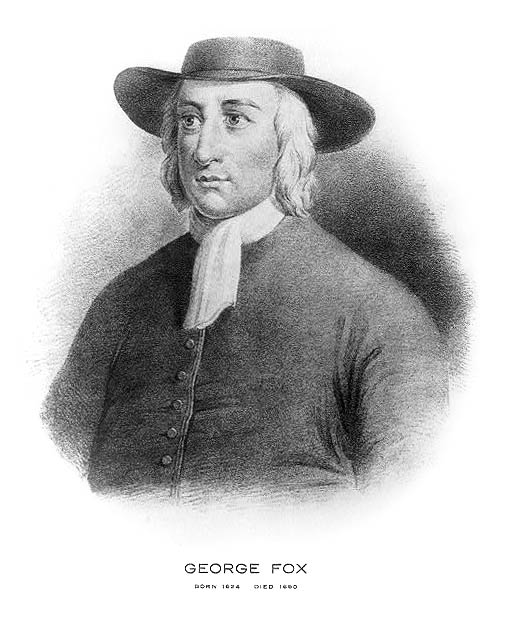
\includegraphics[width=0.20\textwidth]{./pics/Fox-George-LOC.png}
\label{bild:gfox} 
\end{floatingfigure}




Ich wurde geboren im Monat den man Juli nennt\footnote{Fox 
verwarf die üblichen Monatsbezeichnungen als heidnisch.} 1624,
zu Drayton in-the-Clay, in Leicestershire. Mein Vater hieß
Christoph Fox; er war Weber von Beruf, ein ehrbarer Mann,
und es war ein "`Same von Gott"' in ihm. Die Nachbarn
nannten ihn: den "`gerechten Chrtster"'. Meine Mutter war eine
rechtschaffene Frau; ihr Mädchenname war Mary Lago, aus der
Familie der Lago und aus dem Geschlecht der Märtyrer.

In meiner frühesten Kindheit war ich so ernsten und gesetzten
Gemütez, wie es bei Kindern selten ist, so daß, wenn ich Erwachsene 
leichtfertig und ausgelassen mit einander tun sah, ich
einen Abscheu davor in meinem Herzen verspürte und zu mir
sagte: "`Wenn ich einmal ein Mann sein werde, sicherlich werde
ich nicht so leichtfertig tun."'

A1s ich elf Jahre alt war, wußte ich schon was rein und
recht ist; denn ich war als Kind gelehrt worden, wie man rein
bleibt. Der Herr lehrte mich, treu zu sein in allen Dingen, sowohl
innerlich gegen Gott als äußerlich gegen die Menschen; und daß
ich mich in allen Dingen an "`ja"' und "`nein"' halten solle; nicht
wie die Kinder der Welt, die ihren Mund voll List und gleißnerischer
Worte haben, sondern meine Worte sollen: wenig sein, "`lieblich
% \picinclude{./000-009/p_s002.jpg}
und mit Salz gewürzet"' (Col. 4, 6); und daß ich nicht essen
und trinken solle, um mich wollüstig zu machen, sondern um der
Gesundheit willen, jeder Ding dazu gebrauchend, wozu es be-
stimmt ist, zur Ehre dessen, der alleß geschaffen hat [...]

Als ich dann heran wuchs, wollten meine Angehörigen einen
Priester\footnote{Fox bezeichnet mit priest die ordinierteu Geistlichen.} 
aus mir machen. Aber andere rieten zu andrem; so
kam ich zu einem, der seines Zeichens ein Lederhändler war, aber
mit Wolle handelte und Vieh züchtete und verkaufte; und es ging
mancherlei durch meine Hände. Während ich bei ihm war,
war er gesegnet; aber nachdem ich ihn Verlassen, ging es ihm
schlecht und er geriet in Verfall. Während dieser ganzen Zeit
tat ich weder gegen einen Mann noch gegen eine Frau etwas
Unrechtes; denn die Kraft des Herrn war mit mir und bewahrte
mich. Während ich in diesem Dienste stand, gebrauchte ich im
Verkehr das Wort "`wahrlich"', und es war eine übliche Redensart
bei meinen Bekannten: wenn George sagt "`wahrlich"', so kann
ihn nichts umstimmen. Wenn die Buben oder rohe Leute über
mich lachten, kümmerte ich mich nicht um sie, sondern ging meiner
Wege; aber gewöhnlich hatten mich die Leute gern wegen meiner
Geradheit und Ehrlichkeit.

Als ich, noch nicht ganz neunzehnjährig, in Geschäften an
einem Jahrmarkt war, kam mein Vetter, namens Bradford, ein
"`Frommer"' (Professor) und mit ihm noch ein anderer "`Frommer"'
und forderten mich auf, mit ihnen einen Krug Bier zu trinken,
und da ich durstig war, ging ich mit ihnen hinein; denn ich
liebte jeden, der Sinn für das Gute hatte und den Herrn
suchte. Als jeder ein Glas getrunken hatte, fingen sie an, sich
zuzutrinken und verlangten noch mehr, indem sie ausmachten,
daß der, welcher nicht trinken würde, alles bezahlen sollte. Es
betrübte mich, das jemand, der sich für religiös ausgab, solches
tat; sie taten mir sehr weh, denn es war mir dergleichen noch
nie vorgekommen bei keiner Art von Menschen; darum stand ich
auf um zu gehen, indem ich meine Hand in die Tasche steckte,
einen Groschen vor sie aus den Tisch legte und sagte: "`wenn es
so ist, will ich euch Verlassen."' So kehrte ich nach Hause zurück,
aber ich ging in jener Nacht nicht zu Bett, denn ich konnte nicht
schlafen; bald ging ich im Zimmer auf und ab, bald betete und
% \picinclude{./000-009/p_s003.jpg}
schrie ich zum Herrn, welcher also zu mir redete: "`Du siehst, wie
junge Leute zusammengehen in Eitelkeit und alte Leute in die
Erde. Du musst dich von ihnen abwenden und dich von ihnen,
den jungen wie den alten, fern halten und ihnen allen ein
Fremdling werden."'

Darauf, am 9. Tage des 7. Monats 1643,\index{Jahr!1643} verließ ich nach
Gottes Befehl meine Verwandtschaft und brach allen Umgang und
alle Kameradschaft mit jung und alt ab. Ich begab mich nach
Lutterworth, wo ich einige Zeit blieb und von da ging ich nach
Northampton, wo ich mich ebenfalls aufhielt; darauf nach Newport 
Pagnell, von wo ich nach einiger Zeit weiter nach Barnet
ging, im 4. Monat 1644. Als ich nun so das Land durchzog,
wurden die "`Frommen"' (\textit{professors}) auf mich aufmerksam und
wollten mich kennen lernen. Aber ich mied sie; denn ich spürte,
daß sie nicht besaßen, was sie bekannten (\textit{professed}). Während
der Zeit, da ich in Barnet war, kam eine große Anfechtung zu
verzweifeln über mich. Ich sah, wie Christus versucht worden
war, und war in großer Not; bald ging ich nicht aus meinem
Zimmer, und bald wanderte ich einsam durch die Fluren, um auf
den Herrn zu warten.

Ich fragte mich, warum mir solches widerfahren müsse? Ich
prüfte mich und sagte zu mir selber: "`War ich je zuvor so gewesen?"' 
Ich dachte, ich hätte mich vielleicht gegen meine Angehörigen 
verfehlt, weil ich sie verlassen hatte. Ich musste immerwährend 
darüber nachdenken, dass ich solches getan hatte, und
mich fragen, ob ich einem von ihnen ein Unrecht getan hätte;
aber die Anfechtung wurde schwerer und schwerer, und ich wurde
bis zur Verzweiflung versucht. Und weil Satan sein Vorhaben
auf diese Weise nicht erreichte, so legte er mir Fallstricke und
Lockungen, damit ich eine Sünde begehen möchte, die er ausnützen 
könnte, um mich zur Verzweiflung zu bringen. Ich war
etwa 20 Jahre alt, als diese Prüfungen über mich kamen, und
die Angst dauerte mehrere Jahre und ich hätte mich gerne davon
frei gemacht. Ich ging zu manchem Priester, um Trost zu suchen,
aber ich fand keinen bei ihnen.

Von Barnet ging ich nach London, wo ich eine Wohnung nahm,
und dort war ich in großem Elend und Jammer; denn ich sah
daß die großen "`Frommen"' der Stadt alle in den Banden der
Finsternis waren. Ich hatte einen Oheim dort, einen Baptisten,
% \picinclude{./000-009/p_s004.jpg}
die waren damals gottselig (\textit{tender}); dennoch konnte ich ihm meine
Stimmung nicht kundtun, noch mich ihm anschließen, denn ich
durchschaute alle, jung und alt und wie es um sie stand. Etliche
gottselige Leute (\textit{tender people}) hätten mich gern dort behalten,
aber ich getraute mich nicht und wandte mich wieder gegen
Leicestershire; der Gedanke, ich könnte meinen Eltern und Angehörigen 
weh tun, bedrückte mich; denn sie waren, wie ich merkte,
betrübt über meine Abwesenheit.

A1s ich nach Leicestershire kam, wollten meine Leute, das ich
mich verheirate; aber ich sagte ihnen, ich sei noch ein Knabe und
müsse weise werden. Andre hätten mich gerne bei der Hilfstruppe
im Militär\footnote{Es war der Anfang der Bürgerkriege.}
gesehen, aber ich weigerte mich; und es betrübte mich,
das sie mir solche Dinge vorschlugen, denn ich war ein Gottseliger
(tender) Jüngling. Darauf ging ich nach Coventry, wo ich auf
einige Zeit ein Zimmer im Hause eines "`Frommen"' hatte, bis
die Leute anfingen mich zu kennen; denn es waren viele gottselige 
Leute in jener Stadt. Nach einiger Zeit ging ich wieder
in meine Heimat und blieb etwa ein Jahr dort, in großer Trübsal; 
während mancher Nacht irrte ich einsam umher.

Danach kam der Priester von Drayton, Nathanael Stevens,
oft zu mir und ich ging oft zu ihm; und ein anderer Priester
kam oft mit ihm und sie verschmähten nicht, mich anzuhören; ich
stellte ihnen Fragen und diskutierte mit ihnen. Dieser Priester
Stevens stellte mir folgende Frage: warum Christus am Kreuz
gerufen habe: "`mein Gott, mein Gott, warum hast du mich verlassen?"' 
und warum er gesagt habe: "`wenn es möglich, so gehe
dieser Kelch an mir vorüber, aber nicht wie ich will, sondern wie
du willst."' Ich erwiderte ihm, das zu der Zeit die Sünde der
ganzen Menschheit auf ihm gelegen habe und er ihre Missetat
und Übertretung tragen und für sie geopfert und verwundet
werden musste, sofern er Mensch war; aber er starb nicht, sofern
er Gott war; und weil er so für alle starb und den Tod schmeckte
für jeden Menschen, wurde er zum Opfer für die Sünden der
ganzen Welt. So sprach ich, weil ich zu jener Zeit gewissermaßen 
die Leiden Christi, und was er durchgemacht, an mir
nachempfand. Der Priester sagte auch, es sei eine sehr treffende
Antwort, eine, wie er sie noch nie gehört habe. Zu jener Zeit
% \picinclude{./000-009/p_s005.jpg}
pflegte er mich zu loben und anerkennend von mir zu andern zu
sprechen; und das, was ich ihm während der Woche im Gespräch
mitteilte, predigte er dann am \textit{Ersten Tage}\footnote{Fox 
hat den Grundsatz, statt Sonntag, Erster Tag zu sagen, da es für
ihn keine heiligen Tage gibt.}; deswegen mochte
ich ihn nicht leiden. Später wurde dieser Priester ein großer
Verfolger.

Darauf ging ich zu einem andern Priester in Mancetter in
Warwickshire und diskutierte mit ihm über den Grund der Versuchungen 
und der Verzweiflung, aber er verstand meinen Zustand
nicht; er riet mir, zu rauchen und Psalmen zu singen; nun mochte
ich aber den Tabak nicht und zum Psalmensingen war ich nicht
aufgelegt; ich konnte nicht singen. Er lud mich ein, wieder zu
kommen; dann wolle er mir manches sagen; aber als ich kam,
war er ärgerlich und verdrießlich, weil meine früheren Worte ihm
missfallen hatten. Er redete mit seinen Dienstboten über meine
Leiden und Bekümmernisse, und ich bereute, einem solchen meine
Gesinnung aufgedeckt zu haben. Ich sah, das sie alle leidige
Tröster (Hiob 16, 2) waren, und sie machten meine Unruhe noch
größer. Darauf hörte ich von einem Priester, der in der Nähe
von Tamworth lebte und für einen erfahrenen Mann galt. Ich
ging sieben Meilen weit zu ihm, aber ich fand, daß er nur ein
leeres, hohles Gefäß war. Auch von einem Dr. Cradock in Coventry
hörte ich und ging zu ihm. Ich befragte ihn über Versuchung
und Verzweiflung und wie die Anfechtungen wohl über den
Menschen kommen, Er fragte mich, wer Jesu Mutter und Vater
gewesen seien? Ich entgegnete, Maria sei seine Mutter gewesen
und er gelte als der Sohn Josephs, aber er sei der Sohn Gottes.
Wir gingen gerade auf einem schmalen Weg in seinem Garten
und beim Umdrehen trat ich mit dem Fuß auf den Rand eines
Beetes, worüber der Mann in Wut geriet, als ob sein Haut; in
Flammen stünde, und unsere ganze Unterredung war gestört und
ich ging in Bekümmernis hinweg, bekümmerter als ich gekommen
war. Ich sah, das sie alle leidige Tröster waren und so viel
wie nichts für mich, denn sie konnten sich nicht in meinen Zustand
versetzen. Daraufhin ging ich zu einem, namens Macham, einem
Priester von hohem Ansehen. Er verordnete mir Arznei und ich
musste zu Ader lassen. Aber man konnte mir keinen Tropfen Blut
entziehen, weder am Arm noch am Kopf, trotz aller Mühe, die
% \picinclude{./000-009/p_s006.jpg}
man sich gab, weil mein Körper wie ausgetrocknet war
durch Kummer, Unruhe und Jammer, die so schwer auf mir
lagen, das ich hätte wünschen können, gar nicht oder blind geboren 
zu sein, damit ich nie die Schlechtigkeit und Eitelkeit der
Welt gesehen hätte, oder taub, das ich nie eitle und böse Worte
gehört hätte, und wie der Name des Herrn gelästert wurde. Als
die Zeit, die man Weihnacht nennt, kam, ging ich, während andere
sich belustigten und sichs wohl sein ließen, von Haus zu Haus zu
armen Witwen und gab ihnen Geld. Wenn ich zu Hochzeiten eingeladen 
war, wie zuweilen geschah, ging ich nie hin, sondern machte
erst am folgenden Tage oder bald darauf einen Besuch, und wenn
die Leute arm waren, gab ich ihnen Geld; ich besaß davon gerade 
so viel, daß ich niemanden zur Last zu fallen brauchte und
noch dem Dürftigen etwas spenden konnte.

Zu Anfang des Jahres 1646 als ich, auf dem Wege nach
Coventry, mich den Toren der Stadt näherte, stieg die Frage in
mir auf, wie man sagen könne: alle Christen seien Gläubige, sowohl 
Papisten als Protestanten; und der Herr Offenbarte mir,
das, wenn alle Gläubige wären, so wären sie alle aus Gott 
geboren und vom Tode zum Leben durchgedrungen (1. Joh. 3);
nur solche seien wahre Gläubige; und wenn auch andere sagen,
sie seien auch wahre Gläubige, so seien sie es doch nicht.

Ein andermal, als ich am Morgen eines Ersten Tages über
ein Feld ging, offenbarte mir der Herr, das in Oxford oder 
Cambridge erzogen sein noch nicht genüge, um tüchtig und fähig zum
Dienst Christi zu machen; ich verwunderte mich darüber, denn
das war die allgemeine Meinung der Leute. Aber ich sah es
vollständig ein, als der Herr es mir offenbarte und war überzeugt 
davon und pries die Güte Gottes, die mir solches an diesem
Morgen geoffenbart hatte. Es griff das Amt des Priesters Stevens
an, das: "`in Oxford oder Cambridge erzogen zu sein noch nicht
genüge, um tüchtig und fähig zum Dienst Christi zu machen"'; es
wurde mir klar, das das, was mir geoffenbart worden war, das
priesterliche Amt angreife. Meine Angehörigen waren sehr betrübt,
das ich nicht mit ihnen kommen wollte, um den Priester zu hören.
Ich ging eben lieber allein ins Freie mit einer Bibel. Ich fragte sie,
ob nicht der Apostel zu den Gläubigen sage, "`sie bedürfen nicht, das
sie jemand lehre, die Salbung lehre sie"' (1. Joh. 2). Aber wie wohl 
sie wussten, das solches in der Schrift steht, und das es
% \picinclude{./000-009/p_s007.jpg}
wahr ist, waren sie doch betrübt, das ich mich in diesem Punkte
nicht unterwerfen und mit ihnen den Priester anhören konnte.
Ich sah ein, das es ein ander Ding ist, ein wahrer Gläubiger
zu sein, als das worauf es diesen ankommt [...] Warum sollte
ich also diesen anhängen? Weder diesen noch irgendwelchen
Dissentern konnte ich mich anschließen, sondern war allein, ein
Fremdling, und hielt mich einzig an den Herrn Jesus Christus.

Ein andermal hatte ich die Offenbarung, das Gott, der die
Welt gemacht hat, nicht in Tempeln mit Händen gemacht wohne.
Dies schien mir zuerst ein seltsames Wort, denn sowohl die
Priester als auch das Volk pflegten ihre Tempel oder Kirchen
\textit{Stätten der Ehrfurcht}, \textit{heiliger Boden} und \textit{Tempel Gottes}
zu nennen. Aber der Herr zeigte mir deutlich, das er nicht
in diesen Tempeln wohne, die von Menschen verordnet und
ausgerichtet waren, sondern in den Herzen der Menschen. Denn
sowohl Stephanus als der Apostel Paulus gaben Zeugnis,
das er nicht in Tempeln mit Händen gemacht wohne (Art. 7,48),
nicht einmal in demjenigen, den er einst zu bauen befohlen hatte,
sintemal er ihm ein Ende gemacht hatte, sondern sein Volk sei
sein Tempel, und da wohne er. Solches wurde mir geoffenbart,
während ich durchs Feld zu den Meinigen ging. Als ich kam,
sagten sie mir, Priester Stevens sei dagewesen und habe gesagt,
er sei besorgt um mich, weil ich neuen Lichtern nachgehe. Ich
lächelte bei mir selber, im Gedanken was der Herr mir über ihn
und seinesgleichen geoffenbart hatte. Aber ich sagte meinen 
Verwandten nichts davon. Denn obgleich sie den Priester durchschauten, 
gingen sie doch, ihn zu hören, und waren betrübt, das
ich nicht auch ging. Aber ich kam ihnen mit Schriftstellen und
zeigte ihnen, das es eine Salbung gibt im Menschen, die ihn
lehrt, und das der Herr sein Volk selber lehren will. Ich hatte
auch große Offenbarungen über das, was in der Apokalypse steht;
wenn ich davon redete, so sagten die "`Frommen"' und die Priester,
sie sei ein versiegeltes Buch, und wollten mich davon abbringen;
aber ich sagte ihnen, Christus könne die Siegel öffnen und sie
sei das, was uns am nächsten angehe; denn die Briefe seien an
die Heiligen früherer Zeiten gerichtet, aber die Apokalypse handle
von den künftigen Dingen.

Ich traf mit Leuten zusammen, welche die Ansicht hatten,
die Frauen hätten keine Seelen, "`nicht mehr als eine Gans"',
% \picinclude{./000-009/p_s008.jpg}
setzten sie leichtfertig hinzu. Aber ich tadelte sie und sagte ihnen,
das sei nicht recht, denn Maria sage: "`Meine Seele erhebet den
Herrn und mein Geist freuet sich Gottes seines Heilandes"' (Luc. 1,47).

Ein andermal traf ich solche, die Viel auf Träume gaben.
Ich sagte ihnen, wenn sie nicht unterscheiden könnten zwischen
Träumen und Träumen, so würden sie große Verwirrung anrichten; 
denn es gäbe dreierlei Arten von Träumen: erstens:
"`viele Sorgen machen oft Träume"' (Pred. 5,2.); sodann habe der
Mensch oft bei Nacht Einflüsterungen des Satan, und endlich
spreche Gott zum Menschen im Traum. Schließlich ließen auch
diese Leute von solchen Dingen ab und wurden Freunde.\footnote{"`Freubde"' 
ist bis heute die Selbstbezeichnung der Quäker: Das Wort
"`Freund"' ist also hier immer in diesem Sinn zu verstehen.}

Trotz vieler großer Offenbarungen, die ich hatte, kamen doch
oft schwere Anfechtungen über mich, so das ich bei Tag wünschte,
es wäre Nacht, und bei Nacht wünschte ich den Tag. Mit meinen
Offenbarungen war es wie David sagt: \glqq ein Tag sagt es dem
andern, und eine Nacht tut es kund der andern\grqq (Psalm 19,3).
Denn meine Offenbarungen bezogen sich immer eine auf die
andere: sie bezogen sich aber auch auf die Schrift, über die ich
große Offenbarungen hatte, und die Anfechtungen, die über mich
kamen, bezogen sich auch immer eine auf die andere.

Zu Anfang des Jahres 1647 hieß mich der Herr nach
Derbshire gehen, wo ich mit freundlich gesinnten Leuten (\textit{friendly
people}) zusammentraf und ich hatte viele Unterredungen mit
ihnen. A1s ich sodann durch die Gegend des Peak kam, traf
ich noch mehr Gleichgesinnte, worunter aber auch solche, die eitle,
hochfahrende Ideen hatten. In der Gegend von Nottinghamshire
und Leicestershire traf ich ebenfalls Gottselige (\textit{tender people});
unter anderen auch eine sehr gottselige (\textit{tender}) Frau, Elisabeth
Hooton\footnote{Elisabeth Hooten, eine Frau aus den angesehensten 
Gesellschaftskreisen schloss sich später den Quäkern als Predigerin an.}; 
ich hatte mehrere Versammlungen mit ihnen. Aber
meine Trübsal dauerte fort, und ich war oft in großen Versuchungen. 
Ich fastete viel und ging oft manchen Tag draußen
umher an einsamen Orten, und nahm oft eine Bibel und setzte
mich in hohle Bäume und an verlassene Plätze, bis die Nacht
kam; häufig lief ich in der Nacht traurig umher; denn ich war
% \picinclude{./000-009/p_s009.jpg} 
ein Mann der Schmerzen, in den Zeiten, da der Herr sein Werk
in mir anfing.

Während dieser ganzen Zeit hatte ich mich nie mit irgend
jemand zu irgend einer religiösen Richtung Verbunden, sondern
gab mich ganz dem Herrn hin; von aller schlechten Gesellschaft
hatte ich mich losgemacht, hatte Abschied genommen von Vater
und Mutter und allen andern Angehörigen und zog als ein
Fremdling umher, wohin der Herr mein Herz lenkte; ich mietete
ein Zimmer jeweilen in der Stadt, in die ich kam und weilte oft
etwa einen Monat an einem Orte; denn ich wagte nie lange an
einem Orte zu bleiben, da ich fürchtete, als gottseliger Jüngling
sowohl bei den \glqq Frommen\grqq als auch bei den Ungläubigen Schaden
zu nehmen, wenn ich viel mit den einen oder den anderen umging;
darum verhielt ich mich meist wie ein Fremdling; ich suchte himmlische 
Weisheit, und Erkenntnis kam mir einzig vom Herrn. Ich
wurde losgelöst von den äußeren Dingen, um mich allein auf
den Herrn zu verlassen. Meine Prüfungen und Trübsale waren
sehr schwer; aber wenn es mir zwischen hinein etwas leichter
wurde, so geriet ich oft in solch eine himmlische Freude, das ich
wähnte, in Abrahams Schoß gewesen zu sein. Wie ich das Elend,
in dem ich war, nicht schildern kann, ebensowenig kann ich die
Barmherzigkeit beschreiben, die Gott in diesem Elend an mir getan
hat [...]

Nachdem ich die Offenbarung vom Herrn empfangen hatte,
\glqq das in Oxford oder Cambridge erzogen zu sein noch nicht zum
Dienst des Herrn befähige\grqq, achtete ich die Priester weniger und
sah mehr auf die Dissenter; ich sah, das unter diesen einige
Gottseligkeit sei, und viele von ihnen kamen auch später, zu einer
festen Überzeugung, weil sie Offenbarungen hatten. Aber wie
ich die Priester aufgegeben hatte, so ließ ich auch die 
Separatistenprediger und solche, welche als die Erfahrensten angesehen
wurden; denn ich sah, das keiner unter ihnen allen war, der zu meinem
Zustand sprechen konnte. Als alle meine Hoffnungen auf sie und alle
Menschen dahin waren, so das ich nichts hatte, das mir von außen
half, und ich nicht wusste, was tun — da! o da hörte ich eine
Stimme: \glqq es ist Einer, der zu deinem Zustand sprechen kann,
nämlich Jesus Christus.\grqq Und als ich das hörte, hüpfte mein
Herz vor Freude. Dann zeigte mir der Herr, warum niemand
auf der Welt mir in meinem damaligen Zustand helfen konnte,
% \picinclude{./010-019/p_s010.jpg}

nämlich —— damit ihm die Ehre allein gebühre. Alle sind mit
Sünde und Unglauben behaftet, damit Christus, der erleuchtet
und Gnade, Glauben und Kraft gibt, den Vorrang habe [...].
Mein Verlangen nach dem Herrn wurde immer stärker und der
Eifer nach der Erkenntnis Christi und Gottes, ohne jegliche Hilfe
von Menschen oder Büchern. Denn obwohl ich die Schrift las,
die von Gott und Christus sprach, so kannte ich ihn doch nur
durch Offenbarung, als den, der den Schlüssel hat und auftut
(Offb. 3, 7), und als den Vater des Lebens, der mich durch seinen
Geist zum Sohne zog. Dann führte mich der Herr freundlich
weiter und ließ mich seine ewige, unendliche Liebe sehen, die
alles übertrifft, was die Menschen in ihrem natürlichen Zustand,
oder durch Bücher oder die Geschichte erkennen können;
und diese Liebe zeigte mir auch, wie ich selber war ohne ihn.
Ich zog mich zurück von allen anderen, denn durch die Liebe
Gottes sah ich deutlich, wie es um sie stand. Ich hatte keinen
Umgang mit irgendjemand, Priester oder Frommen«, oder
irgendwelchen Separatiften; sondern nur mit Christus, der der
Schlüssel ist, und der mir die Tür zum Licht und zum Leben ge-
öffnet hatte. Jch fürchtete mich vor allem Reden über irdische Dinge;
denn ich sah nur Verderbliches darin, und wie das Leben von Ver-
derben belastet war. Als ich selber in der Tiefe war und unter dem
Druck, da glaubte ich nicht, daß ich je wieder darüber Herr werden
würde; meine Trübsal, Bekümmernis und Versuchung war so
groß, daß ich ost glaubte, verzweifeln zu müssen, so sehr ward
ich versnchet; als aber Christus mir offenbarte, wie er vom gleichen
Satan war versuchet worden, und wie er über ihn Herr geworden
war und ihm den Kopf zertreten hatte (l.Mos. 3, 15), und wie durch
ihn, seine Kraft, sein Licht und seine Gnade und seinen Geist ich
auch siegen werde, da vertraute ich ihm. So war er es, der mir
austat als ich eingeschlossen war und weder Hoffnung noch Glauben
hatte. Christus, der mich erleuchtet hatte, schenkte mir sein Licht,
um daran zu glauben, er schenkte mir Hoffnung, die er selber in
mir ausrichtete, und er gab mir seinen Geist und seine Gnade,
die mir geniigten in meiner Schwachheit. Also erhielt mich der
Herr im tiefsten Elend und Jammer, die oft über mich kamen.
Jch sand in mir zweierlei Durst: nach der Kreatur, um dort
Hilfe und Kraft zu suchen, und nach Gott, dem Schöpfer, und
seinem Sohn Jesus Christus. Jch sah, daß die ganze Welt mir


% \picinclude{./010-019/p_s011.jpg} 

s Erweckung und Krisis bis zum Durchbruch. 11
nicht helfen konnte; wenn ich die Kost, den Palast und die
Dienerschast eines Königs gehabt hätte, so wäre es mir nichts
uütze gewesen; denn nichts konnte mich trösten, als die Kraft
des. Herm. Jch sah, daß die Ptiestet und die ,,Frommen«
und überhaupt die Menschen hohl waren und ganz zufrieden
in dem Zustand, der mich elend machte; und daß sie das
liebten, wovon ich gerne los geworden wäre. Aber der Herr,
von welchem meine Hilfe kam, nahm mein Anliegen auf sich, und
ich wars meine Sorgen aus ihn allein. Darum wartet alle ge-
duldig aus den Herrn, in welchem Zustand ihr auch sein möget;
wartet in der Gnade und Wahrheit, die von Christus kommt;
wenn ihr das tut, so habet ihr eine Verheißung, die der Herr t
an euch erfüllen wird. Wahrlich, selig sind alle, die da hungert
und dürstet nach Gerechtigkeit, denn sie sollen satt werden .....
Wiederum hörte ich eine Stimme, welche sagte: »Du, Schlange,
du suchst das Leben umzubringen, aber kannst es nicht; denn das
Schwert, das den Baum des Lebens (1. Mos. 3.) bewacht, wird
dich umbringen.« Christus, das Wort Gottes, das der Schlange,
dem Mörder, den Kopf zertrat, behütete mich, weil mein Jnneres »
empsänglich war für seinen guten Samen, diesen Samen, der der
Schlange, dem Mörder, den Kopf zertrat. Dieses inwendige
Leben sproßte in mir empor, also daß ich auf alle Einwände der
Priester und der »Frommen« antworten konnte, und brachte mir
Schristworte ins Gedächtnis, um sie zu widerlegen.
Einmal sah ich die große Liebe Gottes und ich wurde mit
Bewunderung über ihre Unendlichkeit erfüllt; ich sah, wer von
Gott ausgestoßen war, und wer ins Reich Gottes einging, und
wie man Einlaß bekommt durch Jesum, der mit seinem himm-
lichen Schlüssel die Tür öffnet; und ich sah den Tod, wie er
über alle Menschen hingegangen war und den Samen Gottes in
den Menschen und auch in mir unterdrückt hatte, wie aber nun
dieser Same in mir ausging und was die Verheißung war. Es
war ein Kampf in meinem Innern: Fragen stiegen in mir
aus über Gaben und Weissagungen; und dann wurde ich
versucht bis zur Verzweiflung, als ob ich gegen den heiligen Geist
gesündigt hätte. Jch war in großer Bangigkeit und Trtibsal
tagelang. Dennoch verließ ich mich ganz aus den Herrn. Ein-
mal als ich von einem einsamen Gang zurückkam, wurde ich so
von der Liebe Gottes eingehüllt, daß ich unaufhörlich die Größe


% \picinclude{./010-019/p_s012.jpg} 
leiner Liebe anftaunen mußte. Während ich in diesem Zustand
war, eröffnete mir die ewige Klarheit und Kraft, daß: ,,alleß ge-
schehen muß in und durch Christum; und daß er jenen Versucher,
den Teufel besiegt und umbringt tmd alle seine Werke und über
ihm steht; und daß alle diese Trübsal gut für mich war, und
die Versuchungen zur Prüfung meineß Glaubenß .dienten, den
C-hristuß mir gegeben. Der Herr schenkte es mir, daß ich durch
alle diese Trübsale und Versuchungen hindurch sehen konnte;
mein lebendiger Glaube wurde erweckt, daß ich sah, wie alleß
durch Christus, daß Leben, geschah, und ich glaubte an ihn. Wenn
irgend einmal meine Stimmung getrübt war, so blieb mein innerer
Glaube fest, und meine tiefgegriindete Hoffnung hielt mich wie
ein Anker im Meere?-grund und ankerte meine unsterbliche Seele
in ihren Bischof (1. Petr. 2,25), indem sie ihr half über den Wassern
der Welt, ihren wilden Wogen, Stürmen und Versuchungen zu
schwimmen. Ach, da wurden mir meine Trübsale, Anfechtungen
und Versuchungen klarer, denn je zuoor. Wenn es Licht ward
in mir, da wurde alleß, waß nicht vom Licht war — Finsterniß
Tod, Versuchung, Unrecht und Gottlostgkeit — offenbar und kam
anß Licht. Darnach entstand ein Feuer in mir, und ich sah »ihn
sitzen wie daß Feuer eineß Goldschmiedß und wie die Seife eineß
Wäscherß«. (Mal. 3, 2). Der Geist der Unterscheidung kam über
mich, durch welchen ich erkannte, maß meine eigenen Gedanken,
mein Seufzen und mein Stöhnen bedeutete, und maß mir die
Erkenntnis trübte, und woher mir die Offenbarungen kamen.
Alleß waß sich nicht in der Geduld bewähren und daß Feuer
nicht erdulden konnte, erkannte ich im Licht alß Seufzer deß
Fleisches, daß sich nicht in Gotteß Willen fügen wollte: dieseß
hatte mich so verdunkelt, daß ich nicht geduldig sein konnte in
Anfechtung, Trtibsal und Verwirrung. Ich konnte mein eigeneß
Jch nicht in den Tod anß Kreuz geben, daß unß die Kraft
verleiht, Gott zu leben; sie bewirkt, daß alleß maß unß
die Gegenwart Christi oerhüllt, maß daß Schwert deß Geisteß
niederschlägt und tötet, nicht weiter leben kann. Jch unter-
schied auch daß Seuszen deß Geisteß, der mir Offenbarungen
eingab und der mich bei Gott vertrat (Röm. 8, 20). Ju diesem
Geiste ist daß wahre Warten im Herrn aus die Erlösung des
Leibeß und der ganzen Kreatur. Durch diesen unsichtbaren Geist,
in dem daß wahre Seufzen geschieht, erkannte ich auch daß ver-



% \picinclude{./010-019/p_s013.jpg} 

Erweckung und Krisi-3 bis zum Durchbruch. 13
kehrte Seufzen und Flehen. Durch diesen unsichtbaren Geist
Unterschied ich in allem, was-«’ ich hörte, sah und schmeckte, das
Falsche, dach sich über den Geist erhebt und ihn dämpst und
betrübt; und ich sah, wie alle die darin waren, im Jrrtum waren
und Schaden nahmete und im falschen Bitten und Flehen und in
jenem Wandeln und Reden, darinnen man Gotteß Namen ver-
geblich anruft; in jenem Geist, der durch das ägyptische Meer
watet und bittet, aber nicht empfängt; denn sie hassen sein
Licht und widerstreisen dem heiligen Geist, sie verwandeln die
Gnade in Wollust und lehnen sich auf wider den heiligen Geist;
und wenden sich ab zoom Glauben, in welchem sie beten sollten,
und vom Geist, in dem sie bitten sollten (Jud.) . . . .
Jch hörte von einer Frau in Laneafhire, die 22 Tage ge-
fastei hatte und ich ging hin, um sie zu sehen; aber alß ich zu
ihr kam, sah ich, daß sie unter großer Versuchung war. Nach-
dem ich zu ihr gereiet von dem, waö ich vom Herrn empfangen
hatte, verließ ich sie denn ihr Vater war ein Großer unter den
,,Frommen«. Von ia ging ich zu den ,,Frommen« in Duckingsield
und Manchester, wo ich einige Zeit blieb und die Wahrheit unter
ihnen verkündete. G3 wurden etliche von ihr überzeugt und nahmen
die Lehre dez Herrn an und wurden durch dieselbe fest gemacht und
blieben in der Wahrheit. Aber die ,,Frommen« waren wütend;
denn sie eiferten alle für die Lehre von der Sündhaftigkeit und
konnten es nicht ertragen, von Vollkommenheit sprechen zu hören
und von einem heilixen, sitndlosen Leben. Aber de; Herrn Macht
war über allen, wenn sie gleich in Finsterniß gebunden waren
und in der Sünde, iiir die sie eiferten und daß- Gottselige in sich
erstickten. GS war zu der Zeit eine große Versammlung der
Baptisten in Brougthon in Leieestershire, mit etlichen, die sich
von ihnen loßgetrenmt hatten; eö gingen auch Leute von anderen
Richtungen hin und ich ging auch; es waren nicht viele Baptisten
aber viele andere dort. Der Herr öfsnete mir den Mund und
die ewige Wahrheit wurde unter ihnen verkündet, und die Macht
dez Herrn war über ihnen allen. Ju diesen Tagen fing die Macht
des Herrn an zu treilsen und ich hatte große Ofsenbarungen über die
Schrift. ES wurdenetliche in dieser Gegend gewonnen und kehrten
sich von der Finstevuiß zum Licht, von der Macht des- Satans zu
Gott, rmd manche werden erweckt zu Gottes Preis-. Ob ich mich an
,,Fromme« oder andere wandte, stets- wurden etliche gewonnen.


% \picinclude{./010-019/p_s014.jpg} 
Ich war damals noch in großen Versuchungen und meine
inneren Leiden waren schwer; aber ich fand keinen, dem ich meinen
inneren Zustand hätte eröffnen können, als allein den Herrn, zu
dem ich Tag und Nacht schrie. Jch ging zurück nach Notting-
hamshire, und dort zeigte mir der Herr, daß das Böse, das sich
in den äußeren Dingen zeigt, inwendig in den Herzen und Ge-
danken unserer bösen Menschennatur ist. Ich sah die Natur der
Hunde, Schweine, Schlangen, die Natur von Sodom und Agypten,
von Pharao, Kain, Jsmael, Esau 2c. inwendig in den Menschen,
während andere sie im Äußern suchten. Jch schrie zum Herrn:
,,Warum muß mir solches geschehen, da ich mich doch nie solchen
Lastern ergeben werde?« Und der Herr antwortete mir, ich
müsse einen Begriff bekommen von diesen Zuständen; wie·sollte
ich sonst zu allen den verschiedenen Zuständen sprechen können?
und ich erkannte die unendliche Liebe Gottes darin. Ich erkannte,
daß es einen Ozean des Todes und der Finsternis gibt, aber
auch einen unendlichen, unerschöpfllichen Ozean des Lichts und
der Liebe, der über den Ozean der Finsternis fließt. Jch sah K
auch darin die unendliche Liebe Gottes, und ich hatte große
Offenbarungen.
Als ich beim Turmhaus (eteeplebouze) 1) von Mansfield vor-
bei kam, sagte der Herr zu mir: ,,Das, was die Leute mit Füßen
treten, muß deine Nahrung sein«. Und während der Herr also
zu mir sprach, offenbarte er mir, daß das Volk und die »Frommen«
das Leben von Christus . . . das Blut des Sohnes Gottes, welches
mein Leben war, mit Füßen treten und von ihren Ginfällen leben,
wenn sie gleich von ihm schwatzen. Gs schien mir zuerst merk-
würdig, daß ich mich nähren sollte mit dem, wa-? die großen
»Frommen« mit Füßen traten; aber der Herr ossenbarte es mir
deutlich durch seinen ewigen Geist und seine Macht.
Die Leute kamen von nah und fern um mich zu sehen;
aber ich vermied, von ihnen ausgesucht zu werden; doch ich mußte
reden und ihnen allerlei eröffnen. Einer, namens Brown, hatte
L große Weissagungen und Gesichte über mich auf dem Totbett.
Er sprach von nichts anderm, als was ich schaffen werde als
1) Fox gebraucht die Bezeichnung ,,Turmhaus« statt Kitche, weil: ,,die
Fechsctzellnnter Kirche nicht ein Gebäude, sondern die Gemeinde der Gläubigen


% \picinclude{./010-019/p_s015.jpg} 

Erweckung und Ktisis bis zum Durchbruch. 15
Werkzeug des Herrn, und von andern sagte er, daß sie in Ver-
derben geraten werden; es erfüllte sich bei einigen, die damals
viel gegolten hatten. Als dieser Mann begraben war, legte sich
die Hand des Herm schwer auf mich, zum Erstaunen vieler, die
glaubten, ich müsse tot gewesen sein; während vierzehn Tagen
kamen viele, nm mich zu sehen. Ich war sehr verändert in Aus-
sehen und Gestalt, als ob mein Körper neu gebildet oder ver-
wandelt worden wäre. Während ich in diesem Zustand war,
schenkte mir der Herr einen Sinn und eine Gabe der Unter-
scheidung, womit ich deutlich erkannte, daß bei vielen, wenn sie
von Gott redeten und von Christus, die Schlange aus ihnen redete;
dies war hatt zu ertragen; doch das Werk des Herrn ging all-
mählich vorwärts, und meine Anfechtungen und Trübsale fingen
an abzunehmen, und Tränen der Freude entrannen mir, so daß
ich Tag und Nacht dem Herrn hätte Freudentränen weinen mögen,
mit demütigem, zerschlagenem Herzen. Jch tat einen Blick in das,
was ohne Ende ist, in Dinge, die nicht ausgesprochen werden
können, und in die Größe und Unendlichkeit der Liebe Gottes,
die sich nicht in Worten ausdrücken läßt; denn ich war durch H
den Ocean der Finsternis und des Todes und durch die Macht
des Satans gebracht worden vermöge der ewigen, herrlichen Kraft
Christi; und selbst durch jene Finsternis wurde ich gebracht, welche
die ganze Welt bedeckt und alles gebunden hält und alle dem Tode
preis gibt. Es war die gleiche Kraft Gottes, die mich durch
solches alles hindurch brachte, welche nachher das ganze Land,
die Priester wie die ,,Frommen« und das Volk ergriff.
Jch konnte von mir sagen, ich sei im geistigen Babylon, Sodom,
Egypten und im Grabe gewesen; aber durch die ewige Kraft Gottes
war ich Herr geworden über jene Mächte und hindurchgedrungen
in die Kraft Christi. Ich sah die Ernte weiß und den Samen
Gottes so dicht im Boden, wie nur je Weizen ausgesäet worden
war, und niemand ihn zu sammeln, darüber trauerte ich mit NT
Tränen.
Es ging das Gerücht über mich, ich sei einer, der den Geist
der Unterscheidung hätte; daraufhin kamen Viele zu mir von nah
und fern, »Fromme«, Priester und Volk. Die Macht des Herm
brach hervor, und ich hatte große Weissagungen; ich redete zu
ihnen von den göttlichen Dingen; sie hörten aufmerksam und an-
dächtig zu, gingen hinweg und machten es ruchbar.


% \picinclude{./010-019/p_s016.jpg} 
Dann kam der Versucher und setzte mir wieder zu und
klagte mich nn, ich hätte wider den heiligen Geist gesündigt; aber
ich mußte nicht, worin. Da kam mir der Zustand Paulus-’ in
den Sinn, wie er in den dritten Himmel verzückt gewesen undf
Dinge gesehen hatte, welche kein Mensch sagen kann, und wie
darauf ein Vote deß Satanß gesandt worden war, ihn mit
Fäusten zu schlagen. So überwand ich durch die Krast Christi
auch diese Versuchung.


%%%%%%%%%%%%%%%%%%% Kapitel 2. %%%%%%%%%%%%%%%%%%%%%%%%%%%%%%
\chapter[Erste Versammlungen]{Erste Versammlungen}

\begin{center}
\textbf{Erste Versammlungen und Proteste.}
\end{center}

Die Macht des Herrn hatte nun, im Jahre 1648\jahr{1648}, schon vielen
die Herzen geöffnet, das sie das Wort des Lebens und der 
Versöhnung aufnahmen. Als ich nun einmal im Hause eines Freundes,
in Nottinghamshire, saß, erkannte ich, das ein großes Krachen
durch die ganze Erde gehen musste und ein großer Rauch 
aufsteigen, überall wo es krachte, und darnach würde ein großes
Beben entstehen: es war die Erde in der Menschen Herzen, die
erbeben musste, bevor der Same Gottes aus der Erde 
hervorgehen konnte. Und so geschah es: die Macht des Herrn fing an,
sie erbeben zu machen, und wir fingen an, große Versammlungen
zu haben, und man spürte die mächtige Kraft und das Wirken
Gottes unter den Leuten, zu ihrer und der Priester Erstaunen [...].

Ich ging nach Mansfield\ort{Mansfield}, wo eine große Versammlung von
\zitat{Frommen} und andern Leuten stattfand; da trieb es mich zu
beten, und die Kraft des- Herrn war so mächtig, das es schien,
als ob das ganze Haus erbebte. Als ich geendet, sagten etliche
der \zitat{Frommen}, es sei gerade wie in den Tagen der Apostel, da
sich \zitat{das Haus bewegte, in dem sie versammelt waren} 
(Act. 2:2\bibel{Act. 02:02@Act. 2:2}).
Nachdem ich gebetet, wollte einer der \zitat{Frommen} beten, aber
dadurch kam eine Trübung und etwas totes über sie und die
andern \zitat{Frommen} wurden betrübt über ihn und sagten, es sei
eine Versuchung über ihn gekommen; darauf kam er zu mir und
bat mich, ich solle wieder beten, aber ich konnte nicht auf 
eineis Menschen Geheis beten\index{Beten!nach Aufforderung}.
Bald darauf war abermals eine Versammlung von \zitat{Frommen}
% \picinclude{./010-019/p_s017.jpg} 
und ein Hauptmann namens Stoddard wohnte ihr bei. Sie
redeten über das Blut Christi\index{Blut Christi}, 
und während sie darüber sprachen,
sah ich durch die unmittelbare Offenbarung des unsichtbaren
Geistes das Blut Christi. Und ich schrie auf und rief: \zitat{Seht
ihr nicht das Blut Christi? Seht in eure Herzen, wie es eure
Herzen und Gewissen besprengt, das sie, los von den toten
Werken, dem lebendigen Gott dienen} (Hebr. 9\bibel{Hebr. 9}). 
Denn ich sah es, das Blut des neuen Testamentes, 
wie es ins Herz kam. Das
erschreckte die \zitat{Frommen}; sie wollten das Blut nur 
auswendig, nicht inwendig haben. Aber 
Hauptmann Stoddard\person{Hauptmann Stoddard} war ergriffen
und sagte: \zitat{Last den Jüngling reden, hört ihn an}, als er sah,
wie sie mich mit vielen Worten zu besiegen suchten.

Es waren auch eine Anzahl Priester da, die für gottselig
galten; einer von ihnen hieß Kellett, und etliche, die empfänglichen
Gemütes waren, gingen hin, um sie zu hören. Es trieb mich,
ihnen nachzugehen, um sie zu ermahnen, auf die Lehre Gottes in
ihrem Inneren zu hören. Damals war der Priester Kellett gegen
das Priesteramt; später jedoch nahm er selbst ein solches an und
wurde ein Verfolger.

Nachdem ich etliche Arbeit getan hatte in dieser Gegend,
ging ich durch Derbshire in meine 
Heimat Leicestershire\ort{Leicestershire}, und
es wurden mehrere, die empfänglich waren, gewonnen. Als ich
von dort weg zog, begegnete ich einer großen Zusammenkunft
von \zitat{Frommen}, die im Freien beteten und die Schrift 
auslegten. Sie reichten mir die Bibel und ich öffnete sie beim 5. Kap.
des Matth.\bibel{Matth. 5}, wo Christus das; 
Gesetz auslegt; und ich erklärte
ihnen den inneren Zustand und den äußeren Zustand worüber sie
in heftigen Streit gerieten und so auseinander gingen; aber die
Kraft des Herrn nahm überhand.

Darauf hörte ich von einer großen Versammlung, die in
Leicester stattfinden würde; es sollte eine Disputation 
geben, die die Presbyterianer\index{Presbyterianer}, 
Independenten\index{Independenten}, Baptisten\index{Baptisten} 
und Common-Payen\index{Common-Payen}
Leute gleicherweise angehen sollte. Die Versammlung war in einem
Turmhause, und der Herr trieb mich, dorthin zu gehen und
zugegen zu sein. Ich hörte ihren Verhandlungen und 
Beweisführungen zu. Einige saßen in Kirchenstühlen und der Priester
war auf der Kanzel; es war eine große Menge versammelt.
Zuletzt tat eine Frau eine Frage über die Stelle bei Petrus:
\zitat{Wiedergeboren aus ewiglichem Samen, aus dem lebendigen Wort
% \picinclude{./010-019/p_s018.jpg} 
Gottes, das ewiglich bleibet} 
(1. Petr. 1\bibel{Petr. 1. 01@1. Petr. 1}). Der Priester sagte ihr:
\zitat{Ich erlaube keiner Frau in der Kirche zu reden,}
\index{Frauenrecht} obgleich er
vorher allen die Freiheit erteilt hatte, zu reden. Da wurde ich
von der Kraft des Herrn übermannt wie in einer Verzückung,
und ich erhob mich und fragte den Priester: \zitat{Nennst du dies
hier, dieses Turmhaus, eine \textit{Kirche}? oder nennst du diese
bunte Menge eine Kirche?}\index{Ekklesiologie} Denn er 
hätte der Frau auf ihre
Frage antworten sollen, nachdem er vorher allen die Freiheit
erteilt hatte, zu reden. Anstatt mir zu antworten, fragte er mich:
was eine Kirche sei. Ich sagte: \zitat{Die Kirche ist der Pfeiler und
Grund der Wahrheit, aus lebendigen Steinen gemacht, aus
lebendigen Gliedern (1. Petr. 2\bibel{Petr. 1. 02@1. Petr. 2}), 
eine geistige Hausgemeinde,
deren Haupt Christus ist; aber er ist nicht das Haupt einer bunten
Menge oder eines alten Hauses aus Kalk, Steinen und Holz.}
Diese Worte brachten alles aus Rand und Band; der Priester
kam aus seiner Kanzel, andere aus ihren Stühlen, und die 
Verhandlungen waren gestört. Ich ging in eine große Herberge und
disputierte dort mit Priestern und \textit{Frommen} aller Richtungen;
und alle waren furchtbar hitzig.\index{Konflikt!theologisch} 
Aber ich bestand auf der wahren
Kirche und ihrem wahren Haupt, trotz ihnen allen, bis sie 
nachgaben und auseinanderstoben. Einer schien sehr geneigt und kam
eine Zeit lang, in der Absicht, sich mir anzuschließen; aber bald
kehrte er sich ganz gegen mich und schloss sich einem Priester an,
trat für die Kindertaufe ein, obgleich er vorher selber ein
Baptist gewesen war, und verließ mich. Aber es wurden an dem
Tage etliche gewonnen; auch die Frau, welche die Frage getan
hatte, wurde gewonnen, samt den Ihrigen; und des Herrn Kraft
und Herrlichkeit leuchtete über allen.

Hierauf kehrte ich zurück nach Nottinghamshire und ging
ink- Vale of Beavor. Unterwegs predigte ich den Leuten Buse
und es wurden viele gewonnen, im Vale of Beavor und in den
Städten; denn ich blieb einige Wochen dort. Eines Morgen?-,
als ich am Feuer sas, kam eine große Wolke über mich, und eine
große Versuchung überkam mich; aber ich blieb ganz ruhig. Und
ich hörte eine Stimme zu mir sagen: »Alle Dinge gehen aus der
Natur heroor«; und die Elemente und die Sterne kamen über
mich, so das ich ganz davon eingehiillt war. Aber die andern
im Hause merkten nichts von all dem, weil ich ganz still und
ruhig war. Und weil ich still und ruhig war und wartete, so


% \picinclude{./010-019/p_s019.jpg} 

Erste Versammlungen und Proteste. 19
stieg eine lebendige Hoffnung in mir auf, und ich Vernahm deutlich
eine Stimme, welche sagte: ,,EZ gibt einen lebendigen Gott, der
alle Dinge geschaffen hat«; und sogleich verschwand die Wolke
und auch die Versuchung, und Leben breitete sich über alles; mein
Herz ward fröhlich und ich prieö den lebendigen Gott. Einige
Zeit darauf traf ich etliche, die behaupteten, es gebe keinen Gott,
sondern alle Dinge gehen aus-3 der Natur hervor. Ich hatte einen
langen Di?-put mit ihnen und brachte sie herum, so das mehrere
zugaben, es gebe einen lebendigen Gott. Da sah ich, das es gut
gewesen war, das ich jene Prüfung durchgemacht hatte. Wir
hatten große Versammlungen in jenen Gegenden, denn die Kraft
des Herm brach hervor in diesem Teil des Landeö. A13 ich nach
Nottinghamshire zurück kam, traf ich eine Schar von verworrenen
Baptisten und andem; die Kraft des Herrn wirkte mächtig und
gewann viele unter ihnen. Darauf ging ich in die Umgegend von
Manöfield, wo die Kraft des Herrn herrlich kund ward, in der
Stadt Mansfield und auch in anderen Städten. Jn Derbshire
wirkte sie in herrlicher Weise. Jn Eton in der Nähe von Derby
war eine Versammlung von Freunden; die Kraft des Herrn tat sich
darin so mächtig kund, das viele gewaltig erschüttert wurden, und
vieler Mund wurde aufgetan durch die Kraft des Herrn. Viele wurden
vom Herrn getrieben in die Turmhäuser zu gehen, zu den Priestern
und zum Volk, um ihnen die ewige Wahrheit zu verkünden.
Einmal als- ich in Man?-field war, fand eine Sitzung der
Richter wegen des Dingenö von Dienstboten statt. ES trieb
mich hinzugehen und den Richtern zu sagen, sie sollten die
Dienstboten richt am Lohn verkürzen. Ich kam in die Nähe
der Herberge, in der die Sitzung abgehalten wurde; aber
alL ich dort eine Musikantenbande traf, ging ich nicht hinein,
sondern gedachte am folgenden Morgen wieder zu kommen, hofsend,
sie dann in ernster Stimmung zu treffen, um mit ihnen zu ver-
handeln; denn es schien mir jetzt nicht die geeignete Zeit. Aber
alö ich am Morgen kam, war alleö fort; da wurde mir ganz
schwarz vor den Augen, so das ich fast nichts mehr sah; ich fragte
den Wirt, wo die Richter an dem Tage Sitzung haben würden;
er sagte mir, in einer etwa acht Meilen entfernten Stadt. Nun
fing ich wieder an zu sehen und lief dorthin, so schnell ich konnte;
altz ich zu dem Hauö kam, in dem sie und ihre zahlreiche Diener-
schaft waren, mahnte ich die Richter, die Dienstboten nicht am



% \picinclude{./020-029/p_s020.jpg} 
Lohn zu verkürzen, sondern ihnen zu geben, was recht und billig
sei, und die Dienstboten ermahnte ich, ihre Pflicht zu tun und
ehrlich zu dienen; sie nahmen meine Mahnungen freundlich auf,
denn ich wurde vom Herm dazu getrieben.
Ferner trieb es mich, an verschiedene Gerichtöhöfe und in ver-
schiedene Turmhäuser in Manöfield und an andern Orten zu gehen,
um alle zu ermahnen vom Unterdrücken und vom Schwören abzu-
lassen und sich von der Ungerechtigkeit zum Herrn zu bekehren und
recht zu tun. Jnsbesondere trieb es mich, nach einer Gerichtsver-
handlung in Manöfield zu einem zu gehen, der einer der schlech-
testen Menschen der dortigen Gegend war, und mit ihm zu reden;
er war ein Säufer und berüchtigte: Mädchenhändler; ich warnte ihn
beim allmächtigen Gott wegen s eines schlechten Wandels; als ich aus-
geredet hatte und ihn Verlassen wollte, lies er mir nach und sagte
mir, während ich mit ihm gesprochen habe, sei er so ergriffen worden,
das ihn seine Kräfte ganz verliesen. So wurde dieser Mann be-
kehrt, und er lies ab von seiner Schlechtigkeit und blieb rechtschaffen
und nüchtern zum Erstaunen aller, die ihn vorher gekannt hatten.
Und das Werk des Herrn nahm zu und viele kamen von der Finster- ,
nie zum Licht, im Laufe dieser drei Jahre 1646, 1647 und 1648.
Es wurden in dieser Zeit mehrere Versammlungen für Freunde ein-
gerichtet, damit Gott sich kund tue durch sein Licht, seinen Geist
und seine Kraft; denn dee Herrn Kraft brach immer herrlicher hervor.
Nun war ich ini Geiste bei Idem stammenden Schwert vorbei
inö Paradies Gotteö eingedrungen. Alle Dinge waren wie um-
gewandelt ftir mich und die ganze Schöpfung hatte einen andern
Geruch für mich, über alles was Worte ausdrücken können. Ich
wuste nur noch von Reinheit, Unschuld und Rechtschaffenheit, denn
ich war erneuert zum Ebenbild Gottes (Col. 3, 10) durch Christus,
in den Zustand, in dem Adam vor dem Fall gewesen war. Die
ganze Schöpfung wurde mir offenbar und es- wurde mir gezeigt,
wie alle Dinge mit dem Namen genannt wurden, der ihrem
Wesen und ihren Kräften entsprach. Ich war unschliisstg, ob ich
nicht sollte Heilkunde treiben zum Nutzen der Menschheit, als ich
sah, wie die Natur und die Kräfte aller Dinge mir so geoffenbart
wurden vom Herrn. Aber alsbald wurde ich ergriffen im Geist
und erkannte einen andern, sicherem Zustand als die Sitndlosig-
keit Adams, den Zustand Jesu Christi, der nicht fallen konnte.
Und der Herr zeigte mir, das die, so ihm treu bleiben im Licht


% \picinclude{./020-029/p_s021.jpg} 
Erste Versammlungen und Proteste. 21
und in der Kraft Christi, erhoben werden in den Zustand, darin
Adam vor dem Fall gewesen war, in welchem die bewunderns-
werten Werke der Schöpfung und ihre Kräfte erkannt werden
können durch die Offenbarung des göttlichen Wortes der Weis-
heit und der Kraft, durch welche sie gemacht waren. Der Herr
führte mich in große Dinge ein, und wunderbare Tiefen wurden
mir geoffenbart, die alles iibertrafen, was Worte beschreiben
können. Aber wer sich dem Geist Gottes unierwirst und hinein-
wächst in das Gbenbild und die Kraft des Allmächtigen, der wird
das Wort der Weisheit empfangen, das alle Dinge offenbar macht,
und wird dazu gelangen, die verborgene Einheit in dem ewigen
Wesen zu erkennen.
So reiste ich umher im Dienste des Herrn, wie mich der
Herr führte. Als ich nach Nottingham kam, war Gottes mächtige
Kraft mit den Freunden. Von da ging ich nach Elawson in
Leieestershire im Tale Veavor, und auch dort wirkte die Kraft
Gottes in Verschiedenen Städten und Dörfern, in denen Freunde
beisammen waren. Während ich dort war, offenbarte mir der
Herr drei Dinge, die sich auf die drei großen Berufsarten in der
Welt — Heilkunde, sogenannte Gottesgelehrtheit und Recht?--H
wissenschast bezogen. Er zeigte mir, das die Ärzte nicht die
Wei?-heit Gottes haben, durch die alle Kreatur geschaffen ist, und
das sie darum ihre Kräfte nicht kennen, weil sie nicht im Worte der
Weis-heit sind, durch das alles gemacht ist. Gr zeigte mir, das
die Priester nicht den wahren Glauben haben, dessen Ursprung
Christus ist; den Glauben, der reinigt und den Sieg gibt und
durch des man Gott gefällt, welches Geheimnis des Glaubens
in reinem Gewissen ist (1. Tim. 3, 9). Gr zeigte mir ferner, das
die Rechtsgelehrten nicht die wahre Villigkeit und Gerechtigkeit
besitzen und nicht das Geses Gottes haben, nach welchem schon
die erste Ubertretung und alle weiteren Sünden gerichtet worden
sind und welches dem Geiste Gottes entspricht, den die Menschen
in sich betrüben und gegen den sie sündigen (Eph. 4, 30).
Und das diese drei, die Ärzte, die Priester und die Rechtsgelehrten,
die Welt ohne Weisheit regieren, ohne Glauben, ohne Billigkeit,
ohne Recht und ohne das Geses Gottes; die einen, indem sie
vorgeben, den Leib zu heilen, die andern die Seele und die dritten
das Eigentum der Leute zu schützen. Aber ich sah, das sie alle
die Weisheit, den Glauben, die Gerechtigkeit und das GesetzZGotteS


% \picinclude{./020-029/p_s022.jpg} 
nicht hatten. Und als der Herr mir diese Dinge osfenbarte, fühlte
ich, das seine Kraft sich über alle ergos und das sie durch die-
selbe alle umgewandelt werden könnten, wenn sie sie aufnehmen und
sich ihr beugen würden. Die Priester würden umgewandelt werden
und zum wahren Glauben kommen, welcher eine Gabe Gottes
ist. Die Rechtsgelehrten würden umgewandelt werden und zum
Geses Gottes (Jar. 2, 2) kommen, welches dem göttlichen im
Herzen entspricht und es möglich macht, seinen Nächsten wie sich
selbst zu lieben. Dieses Geses läst den Menschen erkennen, das
wenn er seinem Nächsten schadet, so schadet er sich selber, und
es lehret ihn, andern zu tun, wie er möchte, das die andern ihm
tun. Die Ärzte können umgewandelt werden und zur Weisheit
Gottes kommen, durch die alle Dinge geschaffen sind, und so
eine rechte Erkenntnis über diese Dinge erlangen und ihre Kräfte
erkennen an den Namen, die die Weisheit, die sie gemacht, ihnen
gab ....
Der Herr offenbaite mir durch seine unsichtbare Kraft, das
ein jeder erleuchtet werde durch das heilige Licht Christi (Joh. 1, 9).
Und ich erkannte, das es in allen leuchtet, und das alle, die
daran glaubten, aus der Verdammnis zum Licht des Lebens
kamen und Kinder des Lichts wurden (Joh. 12, 36). Aber die,
welche es hasten und nicht daran glaubten, die verdammte es, wie-
wohl sie schienen Christum zu bekennen.,« Solches sah ich in der
reinen Offenbarung des Lichts, ohne jegliche menschliche Hilfe;
auch wuste ich damals nicht, wo es in der Schrift zu sinden
war; doch später, als ich in der Schrift forschte, fand ich es.
Damals aber hatte ich jenes Licht und jenen Geist geschaut, welche
gewesen, ehe die Schrift gegeben worden war, und welche die
heiligen Männer Gottes getrieben hatten, die Schrift zu schreiben;
und ich erkannte, das alle, welche Gott, Christus oder die Schrift
recht kennen wollen, zu diesem Geist gelangen müssen. Aber ich
merkte eine Trägheit und faule Schläfrigkeit in den Leuten, die
mich erstaunte; oftmals, wenn ich einschlafen wollte, schweifte
mein Geist über alles hinaus zu dem, der von Ewigkeit zu Ewig-
keit ist. Ich sah, das der Tod über diesen schltisrigen und faulen
Zustand kommen musste, und ich sagte den Leuten, sie müsten
dazu kommen, dieses schläfrige, träge Wesen zu töten und zu
kreuzigen durch die Kraft Gottes, damit ihre Herzen und Sinne
droben seien.


% \picinclude{./020-029/p_s023.jpg} 
Erste Versammlungen und Proteste. 23
Einmal als ich durchs Feld wanderte, sagte der Herr zu mir:
,,Dein Name ist geschrieben im Lebensbuche des Lammeö, welcheö
gewesen vor der Erschaffung der Welt«. Alk- der Herr dies sagte,
da glaubte ich e3 und erkannte es, kraft der neuen Geburt. Einige
Zeit darauf befahl mir der Herr, in die Welt hinaus zu gehen,
die wie eine dornige Wildnis war; und als ich in der Kraft
Gottes mit dem Wort des Lebenö in die Welt hinaus kam, lehnte
sich die Welt dagegen auf und tobte wie die großen tobenden
Wogen der See; Priester wie ,,Fromme«, die Obrigkeit wie das
Volk, alle waren wie die See, als ich kam, den Tag des Herrn
unter ihnen zu verkünden und ihnen Buse zu predigen ......
Als mich Gott und sein Sohn Jesus Christus aussandten
in die Welt, um sein ewigeö Evangelium und Reich zu predigen,
freute ich mich, das ich den Befehl hatte, die Leute jenem innern
Licht, Geist und Gnade zuzuführen, durch die alle ihr Heil und
den Weg zu Gott erkennen können; ja, jenem heiligen Geist,
der in alle Wahrheit führt und von welchem ich bestimmt wuste,
das er nie jemanden trtigt.
Durch diese göttliche Kraft und den Geist Gottes und das
Licht Jesu sollte ich nun die Menschen von ihren eigenen Wegen
ab zu Christus?-, dem neuen, lebendigen Weg bringen; ab von
ihren Kirchen von Menschen gemacht, zur Kirche in Gott, zur
Gemeinde derHeiligen, die imHi1nmel angeschrieben ist (Gbr. 12, 23),
deren Haupt Ehristus ist; ab von den Lehrern dieser Welt, die
von Menschen eingesetzt sind, damit sie von Ehristus:3 lernen, der
der Weg, die Wahrheit und das Leben ist (Joh. 14, 6), von welchem
der Vater sagt: ,,dieS ist mein lisber Sohn, den höret« (Luc. 9, 35);
ab von allem weltlichen Gottezdienst, damit sie den Geist der Wahr-
heit in ihrem Inneren erkennen und sich von demselben führen
lassen; das sie in demselben den Vater der Geister anbeten, dem
solches anbeten angenehm ist; die, welche nicht in diesem Geiste
anbeten, wissen nicht, mas sie anbeten. Ich sollte die Menschen
abbringen von all den Gottesdiensten dieser Welt, welche eitel
sind, damit sie zu dem wahren Gottesdienst kommen, welcher die
Witwen und Waisen in ihrer Trübsal tröstet (Jar. 1, 27) und be-
wahret von der Befleckung der Welt; dann gäbe es:) nicht so viele
Bettler, deren Anblick so ost mein Herz betrübt, weil er von so
viel Hartherzigkeit zeugt unter denen, die vorgeben, C-hristus3 zu
bekennen. Ich sollte sie von allen Gemeinschaften, Singereien


% \picinclude{./020-029/p_s024.jpg} 
und Betereien dieser Welt abbringen, welche Formen ohne Kraft
sind, auf das ihre Gemeinschaft im heiligen Geist sei, im ewigen
Geist Gotteö, und sie darin anbeten und singen, durch die Gnade,
die von Christus kommt; und so dem Herm in ihren Herzen
singen’und spielen, der seinen geliebten Sohn gesandt hat, um
ihr Retter zu sein; der seine himmlische Sonne über und in allen
scheinen läst und seinen himmlischen Regen über Gerechte und
Ungerechte ausgiest (Matth. 5), wie der äusere Regen über alle
fällt und die äusere Sonne fiir alle scheint; dies ist Gotteö un-
aussprechliche Liebe zur Welt. Ich sollte die Leute von den
jüdischen Zeremonien abbringen und von den heidnischen Fabeln
und den menschlichen Einrichtungen und weltlichen Lehren, durch
welche die Leute hin und her von einer Sekte zur andern ge-
trieben werden, und von allen ihren bettelhaften Lehranstalten
und ihren Schulen und Hochschulen, in denen sie Prediger Christi
machen wollen, die aber wahrlich Prediger ihrer eigenen Machen-
schaft sind und nicht Christi; von allen ihren Bildern und Kreuzen
und Besprengen von Kindern; allen ihren sogenannten heiligen
Tagen und nichtigen Traditionen, die sie seit den Tagen der
Apostel eingerichtet haben und gegen welche die Kraft Gottes
sich richtet; vermöge dieser Kraft wurde ich getrieben, gegen
alles das aufzutreten und gegen alle, die nicht umsonst pre-
digten und doch solche waren, die umsonst vom Herrn empfangen
hatten. s
Ferner verbot mir der Herr, als er mich in die Welt hinauö
sandte, meinen Hut abzunehmen vor irgendjemand, hoch oder
niedrig; und ich hatte den Befehl, zu allen, Männern und Frauen,
,,Du« zu sagen, ohne irgend einen Unterschied zu machen zwischen
reich oder arm, gros oder klein; und ich sollte unterwegs- auf
meinen Reisen den Leuten nicht guten Morgen oder guten Abend
sagen, noch mich vor irgendjemand neigen oder das Knie beugen.
Solcheö machte die Sekten und Gemeinschaften zornig. Aber die
Kraft des Herrn half mir durch alles hindurch, zu seiner Ehre,
und viele kehrten sich in kurzer Zeit zu Gott, denn der große
Tag des- Herrn ging auf aus der Höhe und brach eilendö an,
und in seinem Lichte gingen vielen die Augen über ihren Zu-
stand auf.
Aber o, die Wut, in welcher damals- Priester, Obrigkeit,
»Fromme« und andere waren! Aber hauptsächlich die Priester


% \picinclude{./020-029/p_s025.jpg} 
Erste Versammlungen und Proteste. 25
und die ,,Frommen«; denn obgleich das- ,,Du« gegen eine ein-
zelne Person ihrer eigenen Grammatik und Formenlehre, sowie
auch der Bibel entsprach, so konnten sie sich doch nicht drein
finden, es zu hören; und mas die Hut-Ehre anbetraf, das ich
den Hut nicht vor ihnen abnehmen konnte, das machte sie ganz
wütend ....
In jener Zeit fühlte ich mich, zu meiner schweren Prüfung,
auch berufen, in die Gerichtshöfe zu gehen, um nach Gerechtigkeit
zu schreien und die Richter und Behörden in Wort und Schrift
zur Gerechtigkeit zu mahnen; ich musste solche, die öffentliche Gast-
häuser hielten, ermahnen, den Leuten nicht mehr zu trinken zu
geben, als ihnen gut sei; ich musste auftreten gegen ihre Feste
und Gelage, Spiele, Späse und Belustigungen aller Art, durch
die die Leute zur Eitelkeit und Liederlichkeit verleitet und von
der Gottessurcht abgebracht wurden; am häufigsten schändeten
sie Gott (Röm. 2, 23) in dieser Weise an den Tagen, die sie als-
heilige bezeichneten. Auch an Jahrmärkten und Märkten musste
ich mich gegen ihr trügerischeö Handeln wenden, ihren Schwindel
und Betrug; ich musste sie mahnen, die Wahrheit zu sagen, ihr
ja—ja und ihr neinsnein sein zu lassen, und andern zu tun, wie
sie wollten, das man ihnen tue, alles indem ich sie an den großen
Tag des Herrn erinnerte, der über sie alle kommen werde. Auch
gegen allerlei Musizieren und gegen die Schwindler, die in den
Vuden ihr Wesen trieben, musste ich auftreten, denn sie gefähr-
deten die Unschuld und reizten den Sinn der Leute zur Eitelkeit.
Ich musste auch manchen schweren Gang zu Lehrern und Lehrerinnen
tun, um sie zu erinahnen, die Kinder in der Furcht deö Herm zu
erziehen, damit sie nicht in Eitelkeit, Leichisinn und Schlechtigkeit
aufwachsen. Ebenso musste ich Lehrer und Lehrerinnen, sowie die
Väter und Mütter ermahnen, darauf zu achten, das man die
Kinder und die Dienstboten daheim im Hanse zur Gottesstircht an-
halte, damit sie Vorbilder der Tugend und Mäsigkeit werden.
Die irdische Gesinnung der Priester tat mir weh, und wenn
ich die Glocken läuten hörte, welche die Leute inö Turnthaus
rufen sollten, ging es mir durch Mark gund Bein, denn eS war
gerade wie eine Marktglocke, welche die Leute zusammenruft, das I
der Priester seine Ware Izum Verkauf ausbieteu kann. O, die
großen Geldsummen, die zusammenkamen durch ihr Handeln mit
Bibeln und durch ihr Predigen, vom höchsten Bischof biz zum


% \picinclude{./020-029/p_s026.jpg} 
einfachsten Priester! Wa;-’ für ein Handel in der Welt kommt
diesem gleich! Und doch wurde die Schrift gegeben umsonst! Und
Christus hatte seinen Jüngern befohlen, umsonst zu predigen;
und die Propheten und Apostel verkündeten allen geizigen Miet-
lingen und allen, die für Geld iveiösagten, das Gericht. Jch
aber wurde au?-gesandt, in diesem freien Geist das Wort vom
Leben und der Versöhnung umsonst zu predigen, auf das alle zu
Christus kommen, welcher umsonst gibt und in das E-benbild
Gottes erneuert, nach dem Mann und Weib geschaffen waren
vor dem Fall, auf das sie himmlische Güter in Jesus Ehristus
haben möchten.
%%%%%%%%%%%%%%%%%%% Kapitel 3. %%%%%%%%%%%%%%%%%%%%%%%%%%%%%%
\chapter[Tumult in Nottingham]{Tumult in Nottingham}

\begin{center}
\textbf{Der Tumult in Nottingham. Wachsender Widerstand, bis zum
Gefängnis in Derby.}
\end{center}

\section{Tumulte bei dem Gottesdienst in Nottingham}
Als  ich einmal am Morgen eines Ersten Tages in der Nähe
von Nottingham\ort{Nottingham} von einem Hügel aus die 
Stadt überblickte, da
gewahrte ich das riesige Turmhaus, und der Herr sagte zu mir:
\zitat{Du musst hingehen und gegen jene großen Götzen schreien und
gegen die, welche drinnen anbeten}. Ich sagte den \textit{Freunden},
die mit mir waren, nichts davon, sondern ging mit ihnen hin in
die Versammlung, wo die mächtige Kraft des Herrn mit uns
war; hier lies ich sie und ging zum Turmhaus. Die Menge,
die ich hier sah, kam mir vor wie ein Brachfeld und der Priester
wie ein großer Erdklumpen, der oben auf seiner Kanzel stand.
Er hatte zum Text die Worte des Petrus: \zitat{Wir haben ein festes
prophetisches Wort und ihr tut wohl, das ihr darauf achtet, als
auf ein Licht, das da scheinet an einem dunkeln Ort, bis der Tag
anbreche und der Morgenstern aufgehe in eueren Herzen}
(2. Petr. 1:19\bibel{Petr. 2. 01:19@2. Petr. 1:19}). 
Er sagte den Leuten, nach dem, was hier geschrieben 
stehe, sollten sie alle Lehren, Bekenntnisse und Meinungen
prüfen. Da kam die Kraft des Herrn so mächtig über mich und
war so stark in mir, das ich nicht an mich halten konnte, sondern
rufen\index{Gottesdienst!Störung} musste: \zitat{O 
nein, nicht nach dem, was geschrieben stehet!}\index{Exegese}
und ich sagte ihnen, nach was: nämlich nach dem heiligen Geist,
durch den die heiligen Männer Gottes die Schrift geschrieben
haben. Durch diesen, sagte ich, müssen alle Lehren, Bekenntnisse
und Meinungen geprüft werden. Dieser Geist leitet in alle
% \picinclude{./020-029/p_s027.jpg} 
Wahrheit und zur Erkenntnis aller Wahrheit. Die 
Juden\index{Juden} haben
die Schrift gehabt und widerstanden dem heiligen Geist doch und 
verwarfen Christus, den schönen Morgenstern ; sie verfolgten Christus
und seine Apostel und wollten ihre Lehren nach der Schrift prüfen;
aber sie irrten in ihrem Urteil und prüften sie nicht richtig, weil
sie ohne den heiligen Geist prüften. Da ich nun so zu ihnen
redete, kamen die Wachen und führten mich weg und brachten
mich in einen wüsten, stinkenden Kerker; der Geruch stieg mir so
in die Nase und den Hals, das es eine Qual war, aber die
Kraft des Herrn schallte an dem Tage so in ihren Ohren, das
sie ganz von dem Schall betäubt waren, und ihre Ohren wurden
noch eine zeitlang nicht frei davon, so waren sie im Turmhause
von der Kraft des Herrn ergriffen worden. 


\section{Bekehrung des Sheriff John Neckles}

Am Abend brachten
sie mich vor die Behörden der Stadt; als ich vor sie trat, war
der Bürgermeister in verdrieslicher, mürrischer Laune, aber die
Kraft des Herrn beschwichtigte ihn. Sie verhörten mich 
ausführlich und ich berichtete ihnen, wie der Herr mich 
getrieben hatte
zu kommen. Nach einigem Hin- und Herreden schickten sie mich
ins Gefängnis zurück. Aber bald darauf lies mich der Ober-Sheriff,
John Neckles\person{Neckles, John (Sheriff)}, zu sich in 
sein Haus holen. Als ich eintrat, begegnete mir sein Weib 
im Flur und sagte: \zitat{Unserm Hause ist
Heil widerfahren.} Sie reichte mir die Hand und war mächtig
ergriffen von der Kraft Gottes, und ihr Mann und ihre Kinder
und Dienstboten wurden ganz umgewandelt, denn die Kraft des
Herrn war mächtig in ihnen. Ich wohnte bei ihnen und wir
hatten große Versammlungen in ihrem Hause; es kamen auch
etliche angesehene Standespersonen, und des Herrn Kraft tat sich
mächtig kund unter ihnen; John 
Reckles\person{Reckles, John} lies dann einen andern
Sheriff holen und eine Frau, mit der sie in Geschäften zu tun
gehabt hatten, und erklärte in Anwesenheit des andern Sheriff,
das sie beide diese Frau bei einem Handel geschädigt hätten und
sie entschädigen müssten. Er sagte es sehr freundlich, aber der
andere Sheriff leugnete, und die Frau sagte, sie wisse nichts 
davon. Aber der gerechte Sheriff sagte, es sei so, und der andere
wisse das ganz gut; nachdem er die Sache aufgedeckt und das
Unrecht, das sie getan, eingestanden hatte, entschädigte er die
Frau und ermahnte den andern ein gleiches zu tun; die Kraft
Gottes war mit diesem guten Sheriff und wirkte eine große
Wandlung in ihm und er hatte große Offenbarungen. Als er
% \picinclude{./020-029/p_s028.jpg} 
am darauf folgenden Marktag in den Pantoffeln in seinem
Zimmer auf- und abging, sagte er: \zitat{Ich muss auf den Markt
gehen und den Leuten Buße predigen,} und er ging auf den Markt
und in mehrere Straßen und predigte den Leuten Buße; und auch
noch andere aus der Stadt trieb es, zu den Behörden zu gehen
und die Leute zur Buße zu ermahnen. Die Räte wurden sehr
böse über mich und ließen mich aus dem Hause des Sheriff
holen und verurteilten mich zum Gefängnis. Als die 
Gerichtssitzung stattfand, fühlte einer sich 
getrieben, sich statt meiner anzubieten, \zitat{Leib 
um Leib, Leben um Leben}. Als ich vor den
Richter gebracht werden sollte, ging es ziemlich lang, bis mich
der Diener, der mich hinbringen sollte, abholte, und als ich kam,
hatte sich der Richter schon erhoben, woraus ich sah, das er 
erzürnt war; er sagte, er wolle dem Jüngling schon einen Verweis
geben, wenn er vor ihn gebracht werde; ich war damals unter
dem Namen \zitat{Jüngling} eingesperrt. Ich wurde denn wieder
ins Gefängnis gebracht. Die Kraft des Herrn war mächtig
unter den \textit{Freunden}, aber das Volk fing an, tätlich zu
werden, so das der Schloskommandant Soldaten hinaus schickte,
um die Leute auseinander zu treiben, worauf es ruhig wurde;
alle, Priester und Volk, erstaunten ob der herrlichen Kraft, welche
hervorbrach, und etliche der Priester wurden empfänglich gemacht
und einige von ihnen bekannten sich zur Kraft Gottes.

Nachdem ich aus dem Gefängnis von Nottingham, wo ich
einige Zeit gefangen gewesen war, entlassen worden, zog ich
umher, wie vorher im Dienst des Herrn. Als ich 
nach Mansfield\ort{Mansfield}
Woodhouse kam, war dort eine verrückte Frau; das Haar hing
ihr wirr über die Ohren und der Arzt war gerade bei ihr. Er
war daran, ihr zu Ader zu lassen, nachdem man sie zuvor ge-
bunden hatte; viele Leute waren um sie und hielten sie mit Ge-
walt fest, aber man konnte ihr kein Blut entziehen. Ich befahl,
das man sie frei mache und ruhig lasse, denn sie konnten dem
Geiste, der sie plagte, nicht beikommen; sie machten sie srei und
ez trieb mich, zu ihr zu reden und sie im Namen dez Herrn still
und ruhig sein zu heisen, und sie war etz; die Krast dez Herrn
beruhigte ihr Gemüt und sie genaö, und sie nahm die Wahrheit
auf und blieb darin bis zu ihrem Tod. Des Herrn Name wurde
oerherrlichet, ihm gebührt die Ehre aller seiner Werke ....
Während ich in Mansfield Woodhouse war, trieb es mich,


% \picinclude{./020-029/p_s029.jpg} 
Der Tumnli in Nottingham. Wachsender Widerstand usn-. 29
ins Turmhaus zu gehen, um den Leuten die Wahrheit zu ver-
künden, aber das Volk fiel in grosem Zorn über mich her, sie
schlugen mich zu Boden und erstickten mich fast; ich war arg zer-
schlagen und zerquetscht von ihren Händen, Bibeln und Stöcken.
Dann schleppten sie mich hinaus, wie wohl ich kaum fähig war
zu stehen, und taten mich in den Stock, wo ich einige Stunden
sas. Sie brachten Hundepeitschen und Pserdepeitschen und drohten
mir damit. Dann muste ich vor die Behörden im Hause eines
Adligen, wo viele angesehene Leute zugegen waren. Als diese
sahen, wie ich mishandelt worden war, gaben sie mir nach
Vielen Drohungen die Freiheit. Aber der Pöbel trieb mich
zur Stadt hinaus zum Dank dafür, das ich ihnen das Wort des
Lebens verkündet hatte. Ich war kaum imstande zu stehen und
zu gehen, so übel hatten ste mich zugerichtet. Mit groser An-
strengung ging ich etwa eine Meile weit vor die Stadt, wo ich
Leute traf, die mir etwas zur Grquickung gaben, denn ich war
innerlich ganz auseinander, aber die Kraft des Herm heilte mich
bald wieder. Gs waren aber an dem Tage etliche von der Wahr-
heit des Herrn überzeugt worden, worüber ich mich freute. . . .
An einem Ersten Tage kamen wir nach Bagworth und gingen
ins Turmhaus, wohin einige der Freunde gebracht worden waren;
das Volk schlos sie darin ein und sich selbst mitsamt ihrem
Priester. Als der Priester fertig geredet hatte, machten sie die
Türe auf und wir gingen auch hinein und hatten einen Gottes-
dienst mit ihnen, und hernach hatten wir eine Versammlung in
der Stadt, mit manchen angesehenen Leuten. Als ich weiter zog,
hörte ich von solchen, die in Coventry um ihres Glaubens willen
gefangen waren. Aber als ich unterwegs zu ihrem Gefängnis war,
geschah das Wort des Herrn zu mir: ,,Meine Liebe war immer
mit dir und du bist in meiner Liebe«. Und ich fühlte mich ge-
hoben in der Liebe Gottes und sehr gestärkt an meinem innern
Menschen. Als ich in den Kerker zu den Gefangenen kam, über-
kam mich eine grose Finsternis; ich hielt stille, denn mein Geist
ruhte in der Liebe Gottes. Schlieslich singen die Gefangenen
an zu prahlen, und lärmten und lästerten, worüber meine
Seele sehr betrübt wurde. Sie sagten, das sie Gott seien, aber
wir konnten solches nicht ertragen. Als sie ruhig geworden
waren, stand ich auf und fragte sie, ob sie solches aus innerem
Trieb oder auf Grund der Schrift täten? Sie sagten: ,,auf


% \picinclude{./030-039/p_s030.jpg} 
Grund der Schrift.'' Da eine Bibel zur Hand war, hies ich sie,
mir die betreffende Stelle zu zeigen, und sie zeigten mir die Stelle,
wo das Tuch vor Petrus herabgelassen wurde und die Stimme
sagte: ,,WaS Gott gereiniget hat, daö mache du nicht gemein''
(Act. 10, 15). A15 ich ihnen zeigte, das diese Stelle nichts für
sie beweise, brachten sie eine.andere vor, die davon handelte, wie
Gott alle mit sich selbst versöhnt im Himmel und auf Erden
(Col. 1, 20). Ich sagte ihnen, das ich diese Stelle ebenfallö an-
erkenne, das sie aber ebensowenig sür sie passe. Als ich nun
vernahm, wie sie sagten, sie seien Gott, fragte ich sie, ob sie
wissen, ob ez morgen regnen werde? Sie antworteten, das sie
das nicht sagen könnten. Ich erwiderte ihnen: Gott könne das
sagen. Darauf fragte ich sie, ob sie immer so bleiben würden,
wie sie jetzt seien, oder ob sie sich ändern würden? Sie ant-
worteten: sie wüsten ez nicht.'' Ich erwiderte: ,,Gott kann es-
sagen und Gott verändert sich nicht. Jhr sagt, ihr seid Gott und
wist nicht, ob ihr euch verändert oder nicht?« Sie wurden ver-
wirrt und für den Augenblick fast überwunden. Nachdem ich sie
wegen ihrer Gotteslästerungen zurecht gewiesen hatte, ging ich
fort, demr ich merkte, das sie Ranter 1) waren. Ich war nie
mit solchen zuvor zusammengetrosfen und ich priez die Güte des
Herrn, das sie mir erschienen war, ehe ich zu ihnen gekommen
war. Nicht lange nachher schrieb einer dieser Ranterö, namens
Joseph Salmon, ein Buch, in dem er widerrief, worauf sie die
Freiheit erhielten ....
Bei meinem Herumziehen auf den Jahrmiirkten und Märkten
und in den Städten, sah ich Tod und Finsterniö in allen, welche
die Kraft dez Herrn nicht ergriffen hatte. Als ich durch Leieestershire
zog, kam ich nach Twy-Cros; daselbst waren Steuereinnehmer.
Der Herr trieb mich zu ihnen zu gehen und sie zu ermahnen,
sich vor Unterdrückung der Armen zu hüten. Das machte den
Leuten einen grosen Eindruck. GS war in jener Stadt ein ange—
sehener Mann, welcher lange krank gewesen war und von den
Arzten aufgegeben wurde; und etliche Freunde aus- der Stadt
wünschten, das ich zu ihm gehe. Ich ging zu ihm hinauf in sein
Zimmer und sagte ihm das Wort des Lebens, und es trieb mich,
1) Runter, eine Sekte von mystischen Schwürmern, die sich rtihmten,
das Christus in ihnen wohne, aus ihnen rede und sie selbst Christuö seien;
daher der Spottname ,,Ranter«——Prahler.


% \picinclude{./030-039/p_s031.jpg} 
Der Turnnlt in Nottingham. Wachsender Widersnmd usw. 31
mit ihm zu beten. Und der Herr erhörte uns und machte ihn
gesund. Als ich aber darauf in einem untern Raum des Hauses
zu der Dienerschaft und einigen andern Anwesenden redete, stürzte
einer aus einem Nebengemach herein mit dem nackten Degen in
der Hand, gerade auf mich los?-. Ich sah ihn unerschrocken an
und sagte: ,,Wehe Dir, arme Kreatur, was willst Du tun mit
Deiner fleischlichen Waffe? mir ist sie nicht mehr als ein Stroh-
halm.« Die Anwesenden waren sehr bestürzt und er entfernte
sich in Zorn und Wut. Als sein Herr davon hörte, entlies er
ihn auö feinem Dienst. Also beschützte mich der Herr und half
diesem Schwachen und er wurde später den ,,Freunden« sehr
zugetan; und alö ich wieder in jene Stadt kam, besuchte er mich
mit seinem Weibe .....
Als ich nach Derbi) kam, wohnte ich im Haufe eines Arztes?-;
eine Frau wurde gewonnen und noch Viele andere. Als ich in
mein Zimmer ging, läutete die Glocke des Turmhausej-’; nur schon
sie zu hören, ging mir durch Mark und Bein; ich fragte warum
die Glocke läute? man sagte mir, das an dem Tage eine grose
gotteödienstliche Versammlung stattfinde, dazu viele aus dem
Heer, sowie Priester und Prediger kommen werden. Da trieb
es mich, auch hin zu gehen; und alö sie fertig waren, redete ich
zu ihnen, wa?. mir der Herr eingab. Sie waren ziemlich ruhig;
aber eine Wache kam, nahm mich bei der Hand und sagte, ich
müsse vor den Rat sowie auch die andern beiden, die mit mir
waren. Um die erste Nachmittags:-’stunde wurde ich-vorgenommen.
Ich wurde gefragt, warum ich hingegangen sei. Ich sagte, Gott
habe mich getrieben, es zu tun, und weiter sagte ich. ,,Gott
wohnet nicht in Tempeln mit Händen gemacht.« Ich sagte ihnen
ferner, all ihr Predigen, ihr Taufen und ihr Opfern werde sie
nie heiligen, und ermahnte sie, auf Ehristum in ihnen zu schauen
und nicht aus Menschen; denn Christuö sei es, welcher sie heilige.
Darauf ergingen sie sich in Vielen Worten, aber ich sagte ihnen,
sie sollten sich nicht über Gott und Christus streiten, sondern
ihm gehorchen. Die Kraft Gottes donnerte unter ihnen und
sie zerstoben davor wie Spreu. Sie hiesen mich mehrmalö
aus- dem Zimmer gehen und dann wieder hereinkommen und
trieben mich hin und her; von ein Uhr an bis abends neun ver-
hörten sie mich. Zuweilen sagten sie mir mit höhnischen Worten,
ich sei nicht bei Sinnen. Zuletzt fragten sie mich, ob ich geheiligt


% \picinclude{./030-039/p_s032.jpg}
sei; ich antwortete: »Ja, denn ich war im Paradies- Gotte?-,«
(2. Cor. 12, 4). Dann fragten sie mich, ob ich keine Sünde habe.
Ich antwortete: ,,ChristuZ, mein Erlöser, hat die Sünde von mir
genommen und in ihm ist keine Sünde.« Sie fragten, wie ich
wüste, das Christus in uns wohne? Ich sagte: »Durch seinen
Geist, den er unctz gegeben.« Um mich zu versuchen, fragten sie,
ob einer oon uns Christus sei? Ich antwortete: »Nein, wir
sind nichts, Christuö ist alle?-.« Sie sagten: wenn ein Mann
stehle, ob das keine Sünde sei? Ich antwortete: »AlleS Unrecht
ist Stinde.« Als sie ez nun müde geworden, mich zu verhören,
verurteilten sie mich zu sechs Monaten im Korrektionshauö in
Derby alö Gotteölästerer, wie auS folgendem Verhastbesehl zu
ersehen ist:
An den Oberaufseher des Korrektionöhauses in Derby.
,,Hiemit senden wir euch die Personen George Fox, oormals
in Mansfield in der Grafschaft Nottingham, und John Fretwell,
Landwirt, vormals in Staniesby in der Grafschaft Derby, vor
uns gebracht am heutigen Tag und beschuldigt eingestandener
Äuserungen verschiedener gotteölästerlicher Ansichten, die einem
jüngst verfasten Parlament?-beschlus1) zuwider sind; sie sollen daher
sogleich nach Einsicht Dieses aufgenommen werden, besagter
George Fox und Johann Fretwell, in euern Gewahrsam und
darin sicher verwahrt werden, für die Dauer oon 6 Monaten,
ohne Möglichkeit einer Bürgschaft oder Abkürzung, es wäre denn,
das sie sich htulttnglich durch ein gutes Betragen auöweisen, oder
durch unsere eigene Verordnung frei würden. Solcheö zutun
möget ihr nicht versäumen.
Mit unsrer Hand und Siegel gegeben am heutigen Tage
:30. Oktober 1650. Ger. Bennet. «
Nath. Barton.« .....
Während ich im Gefängnis war, kamen oft ,,Fromme«, um eine
Unterredung mit mir zu haben; noch ehe sie etwas sagten, merkte
ich immer, das sie kamen, um für die bleibende Sündhaftigkeit und
Unoollkommenheit einzutreten. Ich fragte sie, ob sie glänbig seien und
11 Partamentöbeschlus vom 2. Mai 1648 gegen GotteHläster11ng und
Ketzerei. Ein Beschlus, der von der unglaublichen Härte der damals regierenden
Pre-zbyterianer zeugt.


% \picinclude{./030-039/p_s033.jpg} 
Der Tnmult in Nottingham. Wachsender Widerstand usw. Z3
Glauben hätten? Sie sagten: ,,Ja.« Jeh fragte sie: in wen?
Sie sagten: ,,J«n Christu-3.« Ich erwiderte: Wenn ihr wahre
an Christus- Glaubende seid, so seid ihr vom Tode zum Leben
eingegangen, und wenn ihr vom Tode frei seid, dann seid ihr ez
auch von der Sünde, die den Tod bringt. Und wenn euer
Glaube wahr ist, so wird er euch den Sieg geben über Sünde
und—Tc-ufel und eure Herzen und Gewissen reinigen — denn der
wahre Glaube ist in reinen Gewissen (1 Tim. 3) und er wird
machen, das ihr Gott gefallet und euch wieder Zugang zu ihm
Verschaffen.« Aber sie wollten nicht von Reinheit und von Sieg
über Sünde und Teufel hören; denn sie sagten, sie können nicht
glaubeny das jemand könne frei von Sünde sein schon diesseits
des Grabe-3. Ich hies sie, da-Z Schwatzen über die Schrift, die
das Wort heiliger Männer sei, aufgeben, wenn sie für Unheiligkeit
eintreten wollten. Einmal kam auch eine Anzahl solcher ,,Frommer«
zu mir und fingen an, die Sündhaftigkeit zu befürworten. Jch
fragte sie: ob sie Hoffnung hätten? ,,Ja, ja! das wäre, wenn
wir keine Hoffnung hötten!« Ich fragte sie: ,,Waö für eine
Hoffnung ist etz, die ihr habt? Jst Christus in euch die Hoffnung
eurer Herrlichkeit? (Col. 1, 27.) Reinigt sie euch, gleich wie er
rein ist?« Aber sie wollten nichtö davon hören, «das sie selber
hienieden schon rein werden sollten. Darauf gebot ich ihnen,
nicht mehr über die Schrift zu reden, welche das Wort heiliger
Männer sei. Denn die heiligen Männer, welche die Schrift ge-
schrieben haben, seien für Heiligkeit in Herz, Leben und Wandel
hienieden eingetreten. ,,Jhr aber«, sagte ich, ,,tretet für Unreinheit
und Sünde ein, die vom Teufel sind, wa-3 habt ihr zu schaffen
mit den Worten heiliger Männer?«
Der Kerkermeister, ein groser ,,Frommer«, hatte eine schreck-
liche Wut auf mich und redete sehr schlecht von mir. Aber etz
gefiel dem Herm, ihn eines Tageö so mächtig zu ergreifen, das
er in groser Angst und innerer Not war. Als ich in meinem
Zimmer umherlief, hörte ich klägliche Laute und hörte, wie er zu
seiner Frau sagte: ,,Frau, ich habe den Tag des Gerichts gesehen,
und George Fox war da, und ich hatte Angst vor ihm, weil ich
ihm so viel böses zugefügt hatte und so vieles wider ihn zu den
Vorgesetzten und ,,Frommen« gesagt hatte und zu den Richtern
und in den Wirt?-häusern.« Hierauf kam er gegen Abend zu mir
ins Zimmer und sagte: »Ich bin gegen euch gewesen wie ein
George Fox- 3


% \picinclude{./030-039/p_s034.jpg} 
Löwe; nun aber komme ich wie ein Lamm und wie der Kerker-
meister, der zitternd zu Paulus und Silas kam.« Und er bat,
das er bei mir bleiben dürfe. Ich sagte, ich sei in seiner Macht
und er könne mit mir machen, was er wolle; aber er sagte:
nein, er wolle meine Grlaubnis haben, und er möchte, das er
immer mit mir sein könnte, aber nicht mich als Gefangenen haben;
er und sein Haus seien meinetwegen geplagt gewesen. Ich erlaubte
ihm denn, bei mir zu sein, und er öfsnete mir sein Herz rmd
sagte, er glaube, das das, was ich vom wahren Glauben und
von der wahren Hoffnung sage, wahr sei, und er wunderte sich,
das der andere, der mit mir gefangen war, nicht dabei bleibe.
Er sagte: ,,Jener andere tat unrecht, ihr aber seid ein Gerechter.«
Er gestand mir auch, das oft, wenn ich ihn gebeten hatte, mich
unter das Volk gehen zu lassen, um ihnen das Wort des Herrn
zu verkünden, und er es mir verweigert habe, habe er sich damit
eine grose Last auferlegt; denn er sei in grose Angst geraten
und einige Zeit ganz verstört und niedergedriickt gewesen, so das
er gar keine Kraft mehr gehabt habe. Am Morgen ging er fort
und ging zu den Richtern und sagte ihnen, wie er und sein Haus
meinetwegen geplagt gewesen seien, und einer der Richter erwiderte
ihm, das auch sie geplagt seien, darum das sie mich sesthielten.
Es war Richter Bennet zu Derby, welcher un-3 zuerst Quäkers)
genannt hatte, weil ich ihnen gesagt hatte, gsie müsten erzittem
vor dem Wort Gottes. Solches geschah im Jahre 1650.
Hierauf erlaubten mir die Richter, eine Meile weit zu gehen.
Joh sah, wo sie hinaus wollten und sagte dem Kerkermeister,
wenn sie mir zeigen wollten, wie weit eine Meile sei, so wolle
ich manchmal so weit gehen; denn ich glaube, sie dachten, ich
würde davon laufen. Und der Kerkermeister gestand nachher,
das sie es in dieser Absicht gestattet hätten, damit ich entkomme
und sie von ihrer Angst befreit würden; aber ich sagte ihm, das
ich nicht diesen Geist habe. «
Dieser Kerkermeister hatte eine Schwester, ein kränkliches
junges Weib. Sie kam zu mir, um mich zu besuchen; und nach-
dem sie einige Zeit bei mir gewesen war, und ich Worte der
Wahrheit zu ihr geredet hatte, ging sie hinunter und sagte den
1) Quüker, das heist ,,Zitterer«, der Spottname, den die Gegner den
Freunden anhängten, wegin der in ihren ersten Versammlungen sich einstellendea
Konvulsionen.


% \picinclude{./030-039/p_s035.jpg} 
Erlebnisse im Gefängnis zu Derbi) usw. Z5
andern, wir seien unschuldige Leute und täten niemand nichts zu
leide, sondern allen nur Gutes, sogar solchen, die uns hasten,
und bat sie, freundlich gegen mich zu sein. ....
Während ich im Korrektionshaus war, besuchten mich meine
Verwandten, und da sie über meine Gefangenschaft bekümmert
waren, gingen sie zu den Richtern und baten sie, das ich mit
ihnen heim gehen dürfe. Sie erboten sich, sich mit hundert Pfund
zu verbiirgen und einige andere aus Derby, die mit ihnen waren,
je mit siinszig Psund, das ich nicht mehr dorthin komme, um
gegen die Ptiestet zu reden. So wurde ich vor die Richter
gebracht, und weil ich nicht einwilligen wollte, das irgendjemand
sich meinetwegen verpftichte, — denn ich war ja keines Vergehens
schuldig und hatte das Wort des Lebens und der Wahrheit ge-
redet, — erhob sich Richter Bennet zornig, und als ich niederkniete, um
Gott zu bitten, ihm zu vergeben, rannte er auf mich los und schlug
mich mit beiden Händen und schrie: »Fort mit ihm! Kerkermeister,
nimm ihn fort!« Hierauf wurde ich wieder in den Kerker gebracht
und muste dort bleiben, bis meine Zeit von sechs Monaten um
war. Aber ich durfte nun eine Meile weit allein gehen, was ich
tat, als ich fühlte, das ich es durfte. Ost ging ich auf den Markt
und in die Strasen und ermahnte die Leute, sich von ihrer
Schlechtigkeit zu bekehren, und ging dann wieder ins Gefängnis.
Und da Leute von allerleiislteligionen mit mir im Gefängnis
waren, ging ich hie und da zu ihnen und wohnte ihren Versamm-
lungen an den Ersten Tagen bei ....
%%%%%%%%%%%%%%%%%%% Kapitel 4. %%%%%%%%%%%%%%%%%%%%%%%%%%%%%%
\chapter[Kampf gegen die Ranter]{Kampf gegen die Ranter}

\begin{center}
\textbf{Erlebnisse im Gefängnis zu Derby. Ein \zitat{Wehe} 
über die Stadt
Lichfield\ort{Lichfield}. Erste Missionsgenossen. Antikirchliche 
Agitation und Kampf gegen die Ranter\index{Ranter}.}
\end{center}


Während ich noch im Gefängnis war, kam ein Soldat zu
mir und erzählte hmir, wie er im Turmhause gewesen sei und dem
Priester zugehört habe, und wie dann auf einmal eine grofze Angst
über ihn gekommen sei und die Stimme des Herrn also zu ihm
geschehen sei: ,,Weißt du nicht, daß mein Diener im Gefängnis
ift? zu ihm gehe und frage ihn um Rat«. Jch redete mit ihm
wie es sein gegenwärtiger Zustand erheischte, und sein Verständnis
zbt


% \picinclude{./030-039/p_s036.jpg} 
wurde geöffnet. Jch sagte ihm, daß der, welcher ihm seine Sünden
ausdecke und ihn um ihretwillen ängstige, ihm auch die Rettung
zeigen werde; denn der dem Menschen die Sünden aufdeckt, ist
derselbe, der sie auch hinwegnimmt. Während ich mit ihm redete,
offenbarte sich ihm der Herr, so daß er anfing, die Wahrheit dez
Herrn und Gorteß Gnade zu erkennen; er fing an, unerschrocken
in seinem Regiment unter den Soldaten von der Wahrheit zu
reden; denn die Schrift wurde ihm mehr und mehr offenbar, und
er ging soweit zu sagen: sein Oberst sei blind wie Nebukadnezar,
daß er den Diener deß Herrn inß Gesängnis werfe. Von da an
hegte sein Oberst einen Groll gegen ihn. Alß im darauffolgenden
Jahre in der Schlacht von Worcester die beiden Armeen neben-
einander lagen, kamen zwei auß der Armee des Könige und
forderten, daß zwei anß der Armee des Parlamentß sich mit ihnen
schlagen sollten; da wählte der Oberst ihn und noch einen, um
der Forderung Folge zu leisten. A13 sein Kamerad im Kampfe
gefallen war, trieb er seine beiden Gegner zur Stadt hinauö, ohne
einen Schuß auf sie abzuseuern; dies erzählte er mir nach seiner
Rückkehr mit eigenem Munde. Nach Beendigung der Schlacht
sah er die Betrügerei und Heuchelei der Offiziere ein, und im
Gedanken daran, wie wunderbar der Herr ihn bewahrt hatte und
waß etz eigentlich um den Krieg sei, legte er die Waffen nieder.
Die Zeit meiner Gefangenschaft war nun fast zu Ende und
da viel neue Soldaten aus-gehoben wurden, so wollten mich die
Kommifsäre zu ihrem Hauptmann machen, und die Soldaten
erklärten, sie wollten keinen andern als mich haben. Der Kerken
meister erhielt den Befehl, mich vor die Soldaten und ihre Vor-
gesetzten aus den Marktplatz zu siihren; dort boten sie mir dieseß
Ehrenamt, wie sie eß nannten, an und fragten mich, ob ich nicht
wolle die Waffen ergreifen für den Commonwealth gegen Karl
Stuart.1) Ich erwiderte ihnen, ich wisse wohl, woher aller
Krieg komme: auö der Begierde, wie schon Jakobus- lehre
(Jak. 4); ich aber stehe in jener Kraft und jenem Leben,
die von vornherein allen Krieg ausschließen. Sie wollten mich
überreden, ihr Anerbieten anzunehmen; sie meinten, ich weigere
mich nur aus Bescheidenheit. Aber ich erklärte ihnen, ich sei in
den Bund des- Friedenö eingetreten, welcher bestanden, ehe es
1) 1651 Schlacht von W1-rceöter zwischen Cron1toell(Con1n1onwealth) und
Karl ll.


% \picinclude{./030-039/p_s037.jpg} 
Erlebnisse im Gefängnis zu Derby usw. 37
Krieg und Zank gab. Sie sagten, sie bieten es mir in Liebe und
Zuneigung an wegen meiner Tugend, und ähnliche Schmeicheleien
mehr. Aber ich sagte ihnen, wenn solches ihre Liebe sei, so trete
ich sie mit Füßen. Da wurden sie zornig und sagten: ,,Nimm
ihn hinweg, Kerkermeister, und wirs ihn in den untersten Kerker
zu den Schelmen und Verbrechern.« Jch wurde weggefiihrt und
an einen wiisten, stinkenden Ort 1) gebracht, wo kein Bett war,
mit 30 Verbrechern, wo ich beinahe ein halbes Jahr gefangen
war, außer, wenn sie mich dann und wann ein wenig in den
Garten ließen, weil sie sicher waren, daß ich nicht davon laufe.
Es hatte damals, als man mich in diesen Kerker gebracht hatte,
geheißen, ich werde wohl nicht mehr heraus kommen. Aber ich
glaubte an Gott und daß ich zu seiner Zeit daraus befreit werde.
Denn der Herr hatte es mir vorausgesagt, daß ich nicht bald
von diesem Ort wegkomme, da ich dort eine Ausgabe für ihn zu
erfüllen habe.
Als es bekannt wurde, daß ich im Kerker von Derby sei, kamen
meineAngehörigen, um mich wieder zu besuchen; denn sie betrachteten
es als eine große Schande für sie, daß ich um der Religion
willen gefangen war; und etliche hielten mich für verrückt, weil
ich für die Reinheit, Gerechtigkeit und Vollkommenheit eintrat.
Unter denen, die zu mir kamen, war einer aus Nottingham,
ein Soldat, der früher Baptist gewesen war. Jin Laufe des Ge-
sprächs sagte er zu mir: »Dein Glaube gründet sich auf einen
Mann, der in Jerusalem gestorben sein soll; solches ist aber nie
geschehen«. Gs betrübte mich sehr, ihn so reden zu hören, und
ich sagte: ,,Wie! hat nicht Christus gelitten vor den Toren Jeru-
salems durch die Juden, die ,,Frommen«, die Hohenpriester und
durch Pilatus?« Aber er leugnete, daß Christus je äußerlich
gelitten habe. Jch fragte ihn, ob denn keine Hohenpriester, keine
Juden, kein Pilatus äußerlich dort gewesen sei? und als er das
nicht bestreiten konnte, sagte ich: ,,So gewiß ein Hohepriester,
ein Pilatus und Juden äußerlich dort gewesen sind, so gewiß ist
Christus äußerlich verfolgt worden von ihnen und hat durch sie
1) Die Zustände der Gefängnisse und Korrektionshäuset im 17. Jahrh.
waren überaus traurig. Überall herrschte große Unreinlichkeit; die Verwaltung
war der Willkür des Gefängnisvotstehers anheim gegeben, der nicht besoldet
war, sondern von den Gefangenen bezahlt wurde, die die Kosten ihres Aufent-
haltes selbst tragen mußten. Vgl. Aschrott, Englisches Gesängniswesen.


% \picinclude{./030-039/p_s038.jpg} 
gelitten«.' Die Reden dieses Menschen veranlaßten eine Ver-
leumdung gegen uns, als ob die Quäker bestritten, daß Christus
gelitten habe und in Jerusalem gestorben sei. Gs war dies ganz
falsch; nie war der leiseste Gedanke daoon in unsern Herzen ge
wesen; es war eine bloße Verleumdung, die uns traf, und die
aus dem Gerede dieses Menschen entstanden war. Derselbe
Mässch behauptete auch, niemals habe irgend ein Apostel oder
Prophet, oder Heiliger oder Mann Gottes äußerlich gelitten; alle
ihre Leiden seien innerlich gewesen; aber ich bewies ihm anBei-
spielen, wie viele unter ihnen gelitten und durch wen sie gelitten;
und so widerlegte die Kraft des Herrn seine oerkehrten Ansichten.
Eine andere Sorte kam zu mir, die behaupteten, sie könnten
Geister unterscheiden. Jch fragte sie, welches der erste Schritt
zum Frieden sei? und in was der Mensch seine Rettung suchen
müsse? Sie fuhren auf und sagten in ihrem Hochmut, ich sei
verrückt; und solche wollten Geister unterscheiden können und
kannten nicht einmal ihren eigenen Geist!
Während dieser Zeit meiner Gefangenschaft geriet ich in
große Bekümmernis über das Vorgehen der Richter und Beamten
in ihren Gerichtshösen. Gs trieb mich, an die Richter zu schreiben,
darum daß sie das Todesurteil fällten wegen allerlei unwichtiger
Vergehen, in Geldsachen oder das Vieh betreffend. Jch mußte
ihnen zeigen, wie solches von jeher dem Gesetz Gottes zuwider
war; ich war deswegen in meinem Geiste sehr betrübt bis inden
Tod, aber da ich mich unter den Willen Gottes stellte, so er-
wachte ein himmlisches Sehnen nach dem Herrn in meinem Herzen,
ich sah den Himmel offen und freute mich und gab Gott die
Ehre ....
Jn diesem Zustande trieb es mich, an die Richter zu schreiben,
wie schädlich es für die Gefangenen sei, so lange im Kerker zu
sein, wie sie da schlechtes von einander lernten, wenn sie mit-
einander über ihre bösen Taten reden. Darum sollten die Urteile
rasch gesprochen werden. Denn ich war ein gottseliger Jüngling
rmd wandelte in der Furcht des Herrn; es betrübte mich, ihre
schlechten Reden zu hören, ich mußte ihnen oft Vorstellungen über
ihre bösen Worte machen und über ihr häßliches Betragen unter-
einander. Die Leute wunderten sich, wie ich bewahrt und behiitet
blieb; denn nie konnten sie mir ein Wort oder eine Tat nach-
weisen, die sie hätten zu meinen Ungunsten auslegen können


% \picinclude{./030-039/p_s039.jpg} 
Erlebnisse im Gefängnis zu Derby usw. 39
während der ganzen Zeit, die ich dort war; denn die unendliche
Kraft des Herrn hielt mich aufrecht und bewahrte mich während
der ganzen Zeit; ihm sei Lob und Ehre immerdar.
Es war eine junge Person mit mir im Gefängnis, die ihrem
Herrn Geld gestohlen hatte. Llls sie zum Tode verurteilt werden
sollte, schrieb ich an den Richter und ans Schwurgericht und
stellte ihnen vor, wie es immer gegen das Gesetz Gottes gewesen
sei, die Leute wegen Diebstahls zum Tode zu verurteilen, und
bat um Gnade. Sie wurde aber doch verurteilt, und man grub
ihr ein Grab und führte sie zur Hinrichtung. D,a schrieb ich noch
einmal ein paar Worte und warnte alle, sich vsor Raubgier und
Habsucht zu hüten, da sie von Gott wegführe, und ermahnte alle
den Herrn zu fürchten, allen irdischen Begierden zu entsagen und
die Zeit zu nützen, dieweil sie da ist; solches hieß ich sie unter
dem Galgen vorlesen. Und obgleich sie sie schon auf der Leiter
hatten, bereit gehenkt zu werden, mit einem Tuch über den Augen,
so wurde sie nun nicht hingerichtet, sondern sie führten sie wieder
zurück ins Gefängnis, und im Gefängnis kam sie nachher dazu,
Gottes ewige Wahrheit zu erkennen.
Es war noch ein anderer Gefangener mit mir, ein schlechter,
gottloser Mensch, ein bertichtigter Schwarzkünstler und Zauberer.
Er drohte, was er alles zu mir sagen und mir tun wolle, aber
er hatte keine Macht, den Mund gegen mich aufzutun. Einmal
gerieten der Kerkermeister und er aneinander und er drohte, er
wolle den Teufel rufen und das Haus niederreißen, so daß der
Kerkermeister Angst bekam. Da trieb mich der Herr hinzugehen
und ihm Einhalt zu gebieten und zu sagen: ,,Komm, laß sehen
was du kannst, tue dein Außerstes«. Jch sagte ihm, der Teufel
sei schon in ihm selber bei uns, die Kraft des Herrn binde ihn
aber. Da schlich er sich davon.
Als nun die Zeit der Schlacht von Worcester kam, sandte
der Richter Vennet Konstabler, um mich zu zwingen, Soldat zu
werden, da er gesehen hatte, daß ich kein Kommando übernehmen
würde. Jch sagte ihnen, ich sei ganz gegen allen äußeren Krieg.
Sie kamen wieder, um mir Werbegeld zu geben, aber ich nahm
es nicht. Daraus wurde ich vor den Wachtmeister Holes gebracht,
der mich eine Weile behielt und dann wieder zurückschickte. Nach
einiger Zeit wurde ich wieder heraufgeholt und vor den Kommifsär
gebracht, welcher erklärte, ich müsse als Soldat gehen, aber ich


% \picinclude{./040-049/p_s040.jpg} 
sagte ihnen, ich sei hiestir tot. Sie sagten, ich sei ja am Leben.
Jch sagte ihnen, wo Neid und Zank sei, da sei Verderben (Jak. 3, 16).
Sie boten mir zweimal Geld an, aber ich wollte nichtß an-
nehmen; daraus wurden sie böse und verurteilten mich zum Ge-
fängnis- ....
Jch war tief betrübt und bearbeitet in meinem Geist während
meiner Gefangenschaft wegen der Schlechtigkeit, die in der Stadt
herrschte; denn obgleich etliche gewonnen waren, so war doch die
Mehrzahl sehr oerhärtet. Jch sah, wie sich das- Außgießen der
Liebe Gotteß von ihnen wegwandte. Ich trauerte über sie, und
es kam über mich, folgende Klage über sie zu verbreiten:
,,O Derby! Wie die Wasser abfließen, wenn die Schleusen
sich öffnen, also fließet die Liebe Gotteß von dir ab, o Derby.
Darum siehe zu, wo du stehest und auf welchem Grund du bist,
ehe du gänzlich verlassen wirst. Der Herr hat mich zweimal ge-
rufen, ehe ich zu dir kam, um gegen deine Eitelkeit und Schlech-
tigkeit aufzutreten und alle zu ermahnen, auf den Herm und
nicht auf Menschen zu sehen. ,,Wehe der prächtigen Krone der
Trunkenen! der welken Blume ihrer Herrlichkeit« (Jes. 28, ll.
Wehe denen, die mit Worten ihren Glauben zur Schau tragen und
doch hochmütig und hochfahrend sind und Unterdrückung und Haß
üben. O Derby! Deine Frömmigkeit und dein Predigen stinken
gen Himmel! Jhr feiert einen Sabbat in Worten und versammelt
euch, um euch schön zu kleiden, ihr frönet der Eitelkeit. Die
Weiber gehen mit aufgerichtetem Halse und geschminkten Ge-
sichtern, wie ez die alten Propheten verurteilt haben (Jes. 3, 16).
Eure Versammlungen sind dem Herrn ein Greuel; ihr erhebet
die Eitelkeit und beuget euch davor; das Laster gedeiht und da-Z
Böse wird geehrt; daö Schlechte wird von den Schlechten ge-
duldet und doch bekennen sie alle Christus mit Worten. O über
die Schlechtigkeit unter euch! EH bricht mir fast das Herz, zu
sehen, wie Gott unter euch verachtet ist, o Derby!«
A18 ich gesehen, wie Gottez Liebe sich von diesem Orte ab-
wandte, wußte ich, daß meine Gefangenschaft hier nun nicht mehr
lange andauern werde, aber ich sah, daß, wenn der Herr mich
srei machen werde, so werde eß sein, wie wenn man einen
Löwen auß seiner Höhle auf die wilden Tiere dee Waldes ab-
läßt. Denn alle »Frommen« hatten eine tierische Gesinnung, die
der Sünde huldigte, so lange sie lebten. Sie waren alle dem


% \picinclude{./040-049/p_s041.jpg} 
Erlebnisse im Gefängnis zu Derby usw. 41
Geist und dem Leben seiud, der in der Schrift gegeben ift und
den sie in Worten bekannten. So geschah ez, wie man hernach
sehen wird.
Ez stand ein Gericht über der Stadt, und den Behörden war
ez unbehaglich meinetwegen; aber sie wußten nicht, waz sie mit
mtr machen sollten. Einmal wollten sie mich vorz Parlament
schicken, ein andermal mich nach Jrland oerbannen. Zuerst
nannten sie mich einen Betrüger und Verfiihrer und Gottes-
lästerer; dann, alz Gott seine Strafe über sie schickte, sagten fie,
ich sei ein ehrlicher, tugendhafter Mensch. Aber ob sie eine gute
oder schlechte Meinung von mir hatten, war mir gleichgültig;
denn weder richtete mich daz eine auf, noch warf mich das andere
nieder, dem Herrn sei Lob. Schließlich mußten sie mich frei
lassen, zu Anfang des Winterz 1651, nachdem ich fast etn Jahr
in Derby gefangen gewesen war, sechz Monate im Zuchthauz
und die übrigen im Kerker.
Alz ich nun wieder meine Freiheit hatte, fuhr ich fort wie
zuvor in der Arbeit für den Herrn und zog im Lande umher,
zuerst in der Gegend meiner Heimat, Leicestershire; ich hielt unter-
wegz Versammlungen, und dez Herrn Geist und Kraft war mit
nur ....
Einmal alz ich mit einigen Freunden unterwegz war und
eine Turmhauzspitze erblickte, ging ez mir durch Mark und Bein;
ich fragte, waz daz für eine Ortschaft sei? ez hieß: Lichfield.
Alsobald erging daz Wort dez Herrn an mich, daß ich dorthin
gehen müsse. Alz wir bei dem Hause angelangt waren, in daz
wir gehen wollten, bat ich die Freunde, die mit mir waren, hinein-
zugehen; ich sagte ihnen aber nicht, wohin ich zu gehen hatte.
Sobald sie im Hause waren, entfernte ich mich und lief über
Hecken und Gräben, biz ich eine Meile weit von Lichsield ent-s
fernt war; da waren auf einem weiten Felde Schäfer, die ihre
Schafe hüteten. Hier befahl mir der Herr, meine Schuhe auzzu-
ziehen; ich zögerte, denn ez war Winter; doch daß Wort dez
Herrn war wie Feuer in mir. So zog ich denn meine Schuhe
aus und ließ sie bei den Schäfern, und die armen Schäfer zitterten
und waren ganz bestürzt. Darauf lief ich wieder eine Meile,
und sobald ich wieder in der Stadt war, erging daz Wort dez
Herrn an mich: ,,Rufe: wehe der blutigen Stadt Lichfield!« Ich
ging also die Straße auf und ab und rief: ,,Wehe der blutigen


% \picinclude{./040-049/p_s042.jpg}
Stadt Lichfield!« Da ez Markttag war, ging ich aus den Markt-
platz, lies aus demselben umher und rief von Zeit zu Zeit: ,,W-ehe
der blutigen Stadt Lichfield!« Und niemand tat mir etwaß.
Während ich rufend durch die Straßen ging, schien es mir, 11lS
ob ein Bach von Blut durch die Straße fließe, und der Markt-
platz kam mir vor wie ein Teich von Blut. Alö ich mich der
mir aufgetragenen Verkündigung entledigt hatte, verließ ich im
Frieden die Stadt. Jch kehrte zu den Hirten zurück, gab ihnen
Geld tmd erhielt meine Schuhe von ihnen zurück. Aber das
Feuer dez Herrn war so in meinen Füßen und in meinem ganzen
Körper, daß mir nichts daran lag, meine Schuhe überhaupt wieder
anzuziehen; und ich wußte nicht recht, ob ich ez tun sollte oder
nicht, bis ich die Grlaubniß dazu vom Herrn fühlte; nachdem ich
meine Füße gewaschen, zog ich meine Schuhe wieder an. Darauf
versiel ich in tiefeß Nachstnnen, warum und aus welchem Grunde
ich wohl gesandt worden sei, gegen diese Stadt zu reden und sie
die ,,blutige Stadt« zu nennen; denn obwohl eine Zeitlang daß
Parlament und eine Zeitlang der König die Herrschaft über diesen
Kirchenspengel gehabt hatte und viel Blut in der Stadt vergossen
worden war während des- Krieges zwischen beiden, so war ez
doch nicht schlimmer gewesen alß an vielen anderen Orten auch.
Nach und nach aber fiel es mir ein, wie zur Zeit dez Kaiserß
Diocletian tausend Christen in Lichsield gemartert worden waren;
darum hatte ich ohne Schuhe durch den Bach ihreß Bluteß gehen
müssen, damit die Erinnerung an das Blut jener Märtyrer, daß
vor mehr als tausend Jahren vergossen worden und in ihren
Straßen erkaltet war, wach werde. Die Nachwirkung jenes Bluteß
war über mich gekommen, so daß ich dem Herrn hatte gehorchen
müssen. Man weiß auö alten Uberlieserungen, wie viel christ-
liche Vriten dort gelitten haben. Ich könnte noch viel berichten
über alle:-’, waß sich mir offenbarte über daß hier während der
zehn Verfolgungen und später vergossene Märtyrerblut, aber ich
überlasse es dem Herrn und seinem Buch, au?7 welchem alleß
gerichtet werden wird; denn sein Buch und fein Geist sind sichere
Uberlieserer.
Darauf zog ich im Lande umher und hatte vielerorts Ver-
sammlungen unter den freundlich Gesinnten. Aber meine Ange-
hörigen waren böse über mich. Nach einiger Zeit kehrte ich nach
Nottinghamshire zurück und ging dann nach Derbshire, um dort


% \picinclude{./040-049/p_s043.jpg} 
Erlebnisse im Gefängnis zu Derby usw. 43
die freundlich Gesinnten aufzusuchen. Jn Yorkshire und an einigen
andern Orten predigte ich Buße: darauf kam ich nach Balby,
wo Richard Famöworth 1) und einige andere gewonnen wurden.
So reiste ich im Lande umher, Buße predigend und daö Wort
dez Herm verkündigend, bis-3 ich in die Gegend von Wakefield
kam, wo James Naylor lebte; er und Thomaß Goodyear
kamen zu mir; beide wurden gewonnen und nahmen die Wahrheit
auf. Auch William Dem?-bury und seine Frau und viele andere
kamen zu mir, wurden gewonnen und nahmen die Wahrheit auf.
Von dort begab ich mich nach Hauptmann PurZloe’S Hauß in
die Nähe von Selby, und besuchte John Leek, der inß Gefängniß
zu mir gekommen war, und er wurde gewonnen. Ich besaß ein
Pferd, mußte mich aber leider davon trennen, da ich nicht wußte,
maß damit anfangen, weil mich der Herr trieb in manches- an-
gesehene Hautz zu gehen, um die Leute zu ermahnen, sich zum
Herrn zu bekehren. Unter anderm trieb mich der Herr auch inß
Turmhauß von Beverly zu gehen, daß damalß eine Stätte beson-
derer Frömmigkeit war; da ich vom Regen ganz durchnäßt war,
ging ich zuerst nach der Herberge. Jn der Türe kam ein junge-3
Weib auf mich zu und sagte: ,,Wie! seid ihr ez? Kommt herein«,
wie wenn sie mich schon gekannt hätte; denn die Kraft dez Herrn
hatte ihr Herz vorbereitet. Ich nahm etwaß zu mir und ging
inß Bett. Am Morgen zog ich meine noch nassen Kleider an
und bezahlte meine Zeche und begab mich ins Turmhauö, wo
einer predigte. A15 er geendet, trieb mich die mächtige Kraft Gotteß,
zu ihnen zu reden, und ich wies sie aus Chrisiuz, ihren Lehrer, hin.
Die Kraft dez Herrn war so mächtig, daß alle von großer Furcht
ergriffen wurden. Der Bürgermeister kam und sprach ein paar
Worte mit mir, aber niemand hatte Macht, mir etwaß zu tun.
Jch verließ die Stadt und ging am Nachmittag in ein anderez
Turmhauß, etwa zwei Meilen weit entfernt. A13 der Priester
geendet, trieb ez mich, eingehend zu ihm und den Leuten über
den Weg deö Lebens und der Wahrheit und den Grund der Gr-
wählung und Verdammung zu reden. Der Priester sagte, er sei
1) Richard Farnsworth, William Dewßbury und James Naylor waren
die ersten bedeutenden Missionsprediger der Quätet. (Näheres s. Weingarten,
Revolutionskirchen Englandtz. S. 218ss.) James Naylor ist in der Geschichte
betiichtigt geworden durch seinen Messiatzeinzug in Bristol, dem Höhepunkt der
saft zum Wahnsinn gesteigerten Schwärmerei des älteren Quälertumö.


% \picinclude{./040-049/p_s044.jpg} 
zu kindlich, um mit mir zu dißputieren; ich erklärte ihm, ich sei
nicht gekommen, um zu di?-putieren, sondern um daß Wort dez
Lebenß und der Wahrheit zu verkünden, und damit sie alle den
Samen kennen lernen möchten, den Gott allen verheißeu, den
Männern wie den Frauen. Die Leute waren hier sehr empfänglich
und wünschten, daß ich wiederkäme an einem Wochentag, um
ihnen zu predigen, aber ich wie:3 sie an ihren Lehrer Jesuö
Christus und verließ sie. Am folgenden Tage ging ich nach
Cranstick zu Hauptmann Pnrßloe, der mich zu Richter Hotham
begleitete. Dieser war ein gottseliger Mann, der auch Gottes
Wirken schon in seinem Herzen verspürt hatte. Nachdem wir eine
Zeitlang über göttliche Dinge geredet hatten, nahm er mich mit
in sein Zimmer und bekannte mir, daß ihm diese Ansichten
schon seit zehn Jahren vertraut seien, und wie er sich freue, daß
der Herr sie nun auch verkünden lasse unter den Leuten. Nach-
her kam noch ein Priester zu ihm, mit dem ich auch über die
Wahrheit redete. Aber der war bald zum Schweigen gebracht,
denn er war ein bloßer Phantaft, der sich daß, wovon er redete,
innerlich nicht angeeignet hatte.
Während ich da war, kam eine angesehene Frau auß Beverly,
um Richter Hotham in irgend einer wichtigen Angelegenheit zu
sprechen. Jin Laufe dez Gesprächeß erzählte sie ihm, daß am
vergangenen Sabbat, wie sie diesen Tag nannten, ein Engel oder
ein Geist in die Kirche von Beverly gekommen sei und herrliche
Dinge von Gott geredet habe zur Verwunderung aller Anwesenden,
und alß er geendet habe, sei er verschwunden; sie wisse nicht, woher
er gekommen, noch wohin er gegangen sei, alle haben sich ge-
wundert, die Priester, die »Frommen« und die Behörden der Stadt.
Richter Hotham erzählte mir das- nachher wieder, woraus ich ihm
mitteilte, daß ich e3 gewesen, der an jenem Tage im Turmhauß
gewesen und die Wahrheit verkündet hatte ....
Am Nachmittag ging ich in ein andereß Turmhauö, wo ein
großer, angesehener Priester, ein Doktor, wie sie ihn nannten,
redete, einer von denen, die Richter Hotham wollte kommen lassen.
Jch ging hin und wartete, biS der Priester geendet hatte. Die
Worte, die er alö Text genommen hatte, waren: ,,Wohlan alle,
die ihr dursiig seid, kommet her zum Wasser, und die ihr nicht
Geld habt, kommt her, kauset und esset, kommt her und kauset
ohne Geld, beide:-3 Wein und Milch (Jes. 55, 1).*- Und der Herr


% \picinclude{./040-049/p_s045.jpg} 
Erlebnisse im Gefängnis zu Derby usw. 45
trieb mich zu sagen: ,,Komm herunter, du Verführer; heißest du
die Leute umsonst kommen und umsonst vom Wasser dez Lebenz
nehmen, und nimmst jährlich dreihundert Pfund dafür, daß du die
Schrift oerkündest? Errötest du nicht vor Scham? Tat der
Prophet Jesaiaß und Christuß, die diese Worte umsonst geredet
und mitgeteilt hatten, auch also? Sagte nicht Christus- zu seinen
Jüngern, alö er sie auösandte zu predigen: umsonst habt ihr ez
empfangen, umsonst gebet etz auch?« Der Priester machte sich
ganz bestürzt davon; nachdem er seine Herde verlassen hatte,
hatte ich so oiel Zeit, alß ich wollte, um zu den Leuten zu sprechen;
ich wieö sie von der Finsternis zum Licht und zur Gnade Gotteß,
die sie lehren und ihnen Rettung bringen werde, und zum Geist
Gotteß in ihrem Jnnern, der sie umsonst lehre.
Dann kehrte ich zu Richter Hothamö Hauß zurück; alß ich
eintrat, schloß er mich in seine Arme und sagte, sein Haus sei
mein Hau-3. Denn er freute sich sehr über daß Werk dez Herrn
und daß seine Kraft kund geworden. Dann erzählte er mir,
warum er am Morgen nicht mit mir zum Turmhauö gegangen
war, und was für Gründe er gehabt hatte; er hatte sich gesagt,
wenn er mit mir in-3 Turmhauß gehe, so würden die Wachen
mich ihm übergeben und da werde er so in die Sache verwickelt;
dann wisse er nicht, maß machen. Darum sei er froh gewesen,
alß Hauptmann Pur?-loe gekommen; aber keiner von ihnen war
in Amts-kleidung gewesen oder hatte den Kragen um den Halß I
gehabt. GZ war damalt-3 etwaß ganz Ungewöhnliche?-, daß einer
ohne Kragen inß Turmhauß kam; aber Hauptmann Purßloe
war ohne einen solchen mit mir ins Turmhauö gekommen, so hatte
die Kraft des Herrn ihn übernommen, daß er gar nicht daran
dachte.
Jch zog weiter und kam an einen Abend zu einer Herberge.
Jch bat die Wirtin, mir etwaß Fleisch zu bringen, wenn sie solches-
habe; aber weil ich »du« und ,,dich« zu ihr sagte, sah sie mich
besremdet an; ich fragte sie, ob sie Milch habe. Sie sagte: nein.
Jch merkte, daß sie nicht die Wahrheit sagte, und um sie noch
weiter zu prüfen, fragte ich sie, ob sie Rahm habe; sie verneinte eö
ebenfalls. Nun stand ein Butterfaß im Zimmer und ein kleiner
Knabe, der daneben spielte, steckte seine Hand hinein und stieß eß
um und oerschiittete allen Rahm vor meinen Augen auf den
Boden; da zeigte es sich, daß die Frau eine Lügnerin war. Sie


% \picinclude{./040-049/p_s046.jpg} 
erschrak, stieß eine Verwünschung aus, hob das Kind auf und
schlug es tüchtig; aber ich machte ihr Vorwürfe wegen ihrer
Lüge und ihres Betrügens. Nachdem der Herr solcherweise ihre
Betrügerei und Bosheit aufgedeckt hatte, verließ ich das Haus
und ging weiter, bis ich zu einem Heuschober kam und brachte
nun die Nacht darin zu im Regen und Schnee, denn es war
drei Tage vor dem Tag, den sie Ehristfest nennen.
f Am folgenden Tage kam ich nach York, wo etliche sehr gott-
selige Leute waren. Am Ersten Tage der darauffolgenden
Woche hieß mich der Herr in das große Münster gehen und zum
Priester Bowles und seinen Zuhörern reden tn ihrer großen
Kathedrale. Jch ging hin und als der Ptiestet geendet, sagte ich,
ich habe ihm und der Gemeinde eine Botschaft von Gott dem
Herrn zu bringen. ,,Dann sage sie schnell!« sagte einer der
,,Frotnmen« aus der Versammlung; denn es war gefroren und
schneite und war sehr kaltes Wetter. Jch sagte ihnen, solches
seiüdas Wort des Herrn an sie: ,,Jhr lebet in Worten, aber der
Herr der Allmächtige verlangt Früchte von euch.« Kaum waren
die Worte aus meinem Munde, so stießen sie mich hinaus und
warfen mich die Stufen hinunter; aber ich stand aus, ohne verletzt
zu sein und ging in meine Wohnung. Etliche wurden überzeugt;
denn schon die Seufzer, die ich ausstieß unter dem Druck und
dem Zwang des Geistes Gottes in mir, genügten, um vieler
i Herzen zu öffnen und zu ergreifen, sodaß sie bekannten, die Seufzer,
die ich ausstoße, machen ihnen Eindruck.; mein ganzes Wesen
war bedrückt davon, daß sie bekannten und nicht besaßen, Worte
machten und keine Früchte brachten.
Nachdem ich für den Augenblick meinen Dienst in York getan
hatte und etliche dort gewonnen worden waren und die Wahrheit
Gottes angenommen und sich zu seiner Lehre bekannt hatten,
verließ ich York und wandte mich nach Cleveland und fand dort
Leute, welche die Kraft Gottes geschmeckt hatten. Ich sah, daß
ein Same in jener Gegend war, und daß Gott dort ein demiitiges
Volk hatte. Unterwegs holte mich, gegen Abend, ein Päpstlicher
ein und redete mit mir über seine Religion und über ihre Gottes-
dienste, und ich ließ ihn alles sagen, was er aus dem Herzen
hatte. Ich brachte die Nacht in einer Schänke zu; am folgenden
Morgen trieb mich der Herr, zu diesem Päpstlichen zu reden. Jch
begab mich in seine Wohnung und zeugte gegen seine Religion


% \picinclude{./040-049/p_s047.jpg} 
Erlebnisse im Gefängnis zu Derbi; usw. 47
und alle ihre abergläubischen Gebräuche und sagte ihm, Gott sei
gekommen, sein Volk selbst zu lehren; das brachte den Papisten
dergestalt auf, daß es ihn aus seinem eigenen Hause trieb ....
Obgleich zu der Zeit der Schnee sehr tief war, fuhr ich fort
herutnzureisen und kam zu einem Marktflecken, wo ich viele
,,Fromme« traf, mit denen ich lange Unterredungen hatte. Ich
stellte ihnen viele Fragen, die sie nicht beantworten konnten, weil
sie sagten, man habe sie noch nie in ihrem Leben so schwere
Dinge gefragt. Von da ging ich nach Stath, wo ich ebenfalls
viele ,,Fromme« und einige Ranter traf. Ich hatte große Ver-
sammlungen unter ihnen undsviele Bekehrungen. Viele nahmen:die
Wahrheit aus, worunter einer, der hundert Jahre alt war; ein
anderer war ein Oberkonstabler und einer war ein Priester, namens
Philipp Scafe. Diesen machte der Herr später durch seinen Geist
zu einem freien Verkündiger seines freien Evangeliums.
Der Priester dieses Ortes war sehr hochfahrend und bedrückte
die Leute sehr mit seinen Abgaben. Wenn sie aus den Fischfang
gingen, so machte er sie Abgaben vom Erlös bezahlen, obgleich
sie dieselben so weit her hatten und sie bis nach Yarmouth zum
verkaufen brachten. Es trieb mich, dort ins Turmhaus zu gehen,
um die Wahrheit zu verkünden und den Priester bloß zu stellen.
Als ich mit ihm geredet hatte und ihm die Unterdrückung des
Volkes vorgestellt hatte, lief er davon. Die Ältesten der Gemeinde
waren sehr hochmiitig und leichtfertig; darum verließ ich sie, nach-
dem ich das Wort des Lebens verkündet hatte, weil sie dasselbe
nicht aufnehmen wollten. Aber das Wort des Lebens, das ich
unter ihnen verkündet hatte, blieb bei etlichen von ihnen, so daß
etliche der Ersten aus der Gemeinde des Nachts zu mir kamen,
und die meisten wurden gewonnen und bekannten sich zur Wahrheit;
so begann die Wahrheit sich in dieser Gegend auszubreiten, und
wir hatten große Versammlungen; dadurch wurden die Priester
zornig und die Ranter fingen an, unruhig zu werden und ließen
mir sagen, sie wollten eine Unterredung mit mir haben, die Priester,
welche Unterdrückung übten, und die Runter. Es wurde ein Tag
festgesetzt und die Ranter erichienen; es kam auch noch ein anderer
Priester, ein Schotte, aber der Priester, welcher sich der Unter-
drückung schuldig gemacht hatte, nicht. Philipp Scafe, der be
kehrte Priester, war bei mir und es erschienen viele Leute. Als
wir uns gesetzt hatten, erklärte ein Ranter, namens T. Bushel,


% \picinclude{./040-049/p_s048.jpg}
er habe ein Gesicht von mir gehabt; ich sei an einem großen Pult
gesessen und er habe kommen müssen und seinen Hut vor mir
abnehmen und sich tief vor mir verbeugen, und er habe eß getan;
und noch viele andere Schmeicheleien sagte er mir. Jch sagte
zu ihm, er habe daß nur erfunden und er solle zu sich selber
sagen: ,,Schäme dich, du Hund«. Er sagte, eß sei nur Neid von
mir, so zu sagen. Darauf fragte ich ihn, waß der Neid eigentlich
sei rmd wie er im Menschen entstehe und waß daß Htindische sei
und wie eß im Menschen entstehe. Denn ich sah genau, daß er
etwaß Hündisrheß hatte, und darum wollte ich von ihm wissen,
wie dieseß Hündische in ihm entstanden sei. ,,Denn«, sagte ich
ihm, ,,mir müssen zuerst von dem reden, maß in unserm Leib
geschieht, ehe wir von dem reden können, roaß außer dem Leibe
ist.« Damit stopfte ich ihm daß Maul und allen seinen Runter-
genossen, denn er war ihr Haupt. Dann ries ich den Priester,
welcher die Leute unterdrückte, aber er kam nicht; nur der schottische
Priester erschien, der mit wenig Worten zum Schweigen gebracht
war; denn eß war innerlich kein Leben in ihm von dem, waß er-
bekannte. Nun war die Gelegenheit da, mit den Leuten zu reden.
Jch zeigte klar, wie die Ranter waren und verglich sie mit den
Prahlern in Sodom. Jch zeigte, wie ihre Priester die gleiche
Sorte von Mietlingen seien, wie die falschen Propheten früherer
Zeiten, und wie die Priester damals daß Volk auch in dieser
Weise regierten, indem sie ihren Gewinn im Auge hatten und
um Geld ihr Amt besorgten und um schnöden Gewinnß willen
lehrten. Jch stellte Christuß und die wahren Propheten und die
Apostel den Priestern gegenüber und zeigte, wie Ehristuß, die
Propheten und die Apostel sie schon lange an ihren Früchten
erkannt hätten. Dann wieß ich sie aus den Lehrer in ihrem
Jnnern hin, Jesus Christuß, ihren Heiland. Und ich predigte
Christuß in den Herzen, nachdem ich alle diese Höhen geebnet
hatte. Die Leute waren alle ruhig und die Widersacher zum
Schweigen gebracht. Denn obgleich eß innerlich in ihnen kochte,
so hielt die Kraft sie doch gebunden, so daß sie nicht loßbrechen
konnten .....
Ein anderer Priester ließ mich holen, um mit mir zu reden,
und etliche ,,Freunde« gingen mit mir nach seinem Hauö. Alß
er hörte, daß wir gekommen seien, entwischte er auß dem Hause
und versteckte sich unter einer Hecke. Die Leute gingen, ihn zu


% \picinclude{./040-049/p_s049.jpg} 
Erlebnisse im Gefängnis zu Derby usw. 49
zu suchen und fanden ihn, aber sie brachten ihn nicht dazu, zu
uns zu kommen. Daraus ging ich in ein nahegelegenes Turm-
haus, wo der Priester und das Volk in großer Erregung waren,
denn eben dieser Priester hatte den Freunden mit allem Ntöglichen,
das er tun werde, gedroht; als ich aber kam, machte er sich davon,
denn die Kraft des Herrn kam über ihn und über die andern.
Ja, des Herrn ewige Kraft kam über die Erde und drang zu
den Herzen der Menschen und machte die Priester und die
,,Frommen« zittern. Sie machte die Geister der Erde und der
Lust erbeben, zu welchen sie Vorgaben zu beten, sodaß sie einen
Schreck bekamen, wenn es hieß: »Der Mann in den ledernen
Kleidern kommi!«1) An vielen Orten machten sich die Priester,
wenn sie das hörten, davon, so waren sie von Furcht vor der
ewigen Kraft Gottes ergriffen .....
Von hier gingen wir über Scarbvrough .... nach Malton .....
Am Ersten Tag kam eine Frau, eine der angesehensten ,,Frvmmen«
unter den Jndependenten, welche ein solches Vorurteil gegen mich
hatte, daß sie sagte, ehe sie kam, sie würde sich freuen, mich er-
hängt zu sehen; aber als sie kam, wurde sie gewonnen und ge-
hört seither zu den »Freunden«.
Daraus hatte ich hier große Versammlungen; es hätten noch
mehr Leute daran teil genommen, aber sie wagten es nicht, aus
Furcht vor ihren Angehörigen. Es wurde damals als etwas
Unerhörtes angesehen, daß man in Häusern predigte statt in der
,,Kirche«, wie sie es nannten; darum wurde sehr gewünscht, daß
ich ins Turmhaus gehe und ddrt rede. Einer der Priester schrieb
mir und lud mich ein, im Turmhaus zu predigen, und nannte
mich seinen Bruder. Ein anderer Priester, eine bekannte Persön-
lichkeit, hielt dort eine Stunde. Nun hatte mir der Herr während
meiner Gefangenschaft in Derby kund getan, ich solle in den
Turmhäusern predigen, um die Leute von denselben abzubringen,
und es kamen mir auch zuweilen Bedenken wegen der Kanzeln,
in denen die Priester herumsaulenzten. Die Turmhäuser und
Kanzeln verletzten mein Gefühl, weil sowohl die Priester als auch
das Volk sie Gotteshäuser nannten und im Wahne waren, daß
Gott da in äußern sichtbaren Häusern wohne, statt im Gegenteil
1) Fox trug immer Kleider aus Leder, die et wegen ihrer Einfachheit und
Dauerhaftigkeit allen andern Kleidungsstiicken vorzog. (Vgl. Carlyles, Surtor
Resartus: Ein Ereignis in der neuen Geschichte.)
George Fox. 4


% \picinclude{./050-059/p_s050.jpg} 
Verlangen zu tragen, daß Gott und Christus in ihren Herzen
und Leibern wohne, aus daß sie Tempel Gottes? würden. Denn
der Wostel sagt: ,,Gott wohnet nicht in Tempeln mit Händen
gemacht'' (Act. 7, 48). Weil man aber diese Stätten nun einmal
heilig hielt, so fand man ez- schrecklich, wenn man etwas dagegen
sagte. A18 ich inZ Turmhauß kam, waren nicht mehr altz 11 Zu-
hörer dort, und der Priester hielt ihnen die Predigt. Alß nun
in der Stadt bekannt wurde, ich sei im Turmhause, so füllte sich
daßselbe bald mit Menschen. Alk- der Priester, der an dem Tage
zu predigen hatte, geendet hatte, hieß er den andern Priester, der
mich aufgefordert hatte zu kommen, mich auf die Kanzel führen,
aber ich ließ ihm sagen, ich brauche nicht auf eine Kanzel zu
steigen. Darauf ließ, er mir wieder sagen, er wünsche aber, daß
ich sie befteige, weil dort ein besserer Platz sei, an dem mich die
Leute sehen könnten. Ich ließ ihm darauf sagen, man sehe mich
gut genug, da wo ich sei, ich sei nicht gekommen, solche Stätten
noch aufrecht zu erhalten und ihr Bestehen und den Handel, der
damit getrieben wird. Alk- ich dieö gesagt hatte, fingen sie an,
böse zu werden und sagten: ,,Da8 sind die falschen Propheten
der letzten Zeiten«. Diese Rede Verletzte etliche und sie murrten
darüber; nun stand ich auf und hieß alle ruhig sein; ich stieg
auf einen hohen Stuhl und erklärte ihnen, woran man die falschen
Propheten erkenne, und daß sie schon gekommen seien; und dann
zeigte ich ihnen im Gegensatz dazu die wahren Propheten, Christus-
und die Apostel. Ich wieß sie alle an ihren inneren Lehrer,
Christue, der sie von der Finsterniö zum Lichte führen könne.
Nachdem ich ihnen verschiedene Schriftstellen erklärt hatte, wies
ich sie auf den Geist Gottes in ihren Herzen hin, durch welchen
sie zu ihm kommen könnten und erkennen, wer die falschen
Propheten seien. Nachdem ich so ein reiches Wirken unter ihnen
gehabt hatte, zog ich im Frieden von dannen ....
Hierauf kam ich nach Pickering, wo die Richter im Turm-
hauö ihre Sitzungen hielten; Ftiedenztichtet Robinson war Vor-
sitzender. Ich hatte zur gleichen Zeit eine Versammlung im
Schulhaus und viele »Fromme« und Priester wohnten ihr bei
und stellten allerlei Fragen, die zu ihrer Zufriedenheit beantwortet
wurden. ES war gerade die Zeit der Gerichtösit-zungen, und da
wurden auch vier Oberkonstabler bekehrt. GS kam Richter Robin-
son zu Ohren, daß der Priester, den er allen andern Priestern


% \picinclude{./050-059/p_s051.jpg} 
Erlebnisse im Gefängnis zu Terby usw. 51
oorzog, besiegt und überzeugt worden war. Wir gingen nach
der Versammlung in eine Herberge; Richter Robinson’s Priester
war sehr bescheiden und lieb und wollte sogar durchaus mein
Essen bezahlen, was ich aber nicht zuließ. Dann bot er mir sein
Turmhaus an, um darin zu predigen, aber ich lehnte es ab und
erklärte ihm und den andern, daß ich eben gekommen sei, um die
Leute oon diesen Dingen ab und zu Christus zu bringen.
Am folgenden Morgen ging ich mit den vier Konstablern und
andern, um Richter Robinson zu besuchen, der mir unter der
Türe seines Zimmers entgegenkam. Jch sagte ihm, ich könne ihm
keine menschliche Ehre erweisen; er sagte, er sehe nicht aus das.
Jch ging nun mit ihm ins Zimmer und tat ihm den Unterschied
zwischenswahren und falschen Propheten dar, und wie die wahren
höher stehen als die falschen, und richtete seinen Sinn aus
Christum seinen Lehrer. Jch deutete ihm die Gleichnisse, und
wie es sich mit der Grwählung und Verwersung verhalte, wie
man in der ersten Geburt in der Verwersung sei und in der
zweiten in der Grwählung. Ich zeigte ihm, wer die Verheiß-ungen
Gottes habe und wen sein Gericht verdamme. Gr gab alles zu
und war so offen für die Wahrheit, daß, wenn ein anderer an-«
wesender Richter eine kleine Ginwendung machen wollte, er ihn
belehrte. Beim Fortgehen sagte er, ich tue sehr gut, diese mir
von Gott verliehene Gabe zu gebrauchen. Gr nahm den obersten
Konstabler beiseite und wollte ihm etwas Geld siir mich geben,
weil er nicht wollte, daß ich in ihrer Gegend irgend welche Aus-
gaben habe; aber sie sagten ihm, daß ich nicht dazu zu bringen
sei, etwas anzunehmen. Jch schätzte seine Freundlichkeit, das
Geld jedoch lehnte ich ab.
Jch zog im Lande umher und der Priester, der mich Bruder
genannt hatte, zog mit mir. Als wir in eine Stadt kamen, wo
wir im Sinne hatten etwas zu essen, läuteten die Glocken.
Jch fragte, warum sie läuten; man sagte mtr, sie läuten für mich,
damit ich im Turmhaus predige. Bald daraus trieb es mich
dorthin. Als ich kam, sah ich die Leute auf dem Turmhausplatze
versammelt; der alte Priester wollte, daß ich ins Turmhaus gehe,
  ich sagte, es sei nicht nötig. Ge besremdete die Leute, daß
ich nicht in das gehen wollte, das sie ,,Goiteshaus« nannten. Jch
stellte mich auf den Platz des Turmhauses und erklärte den Leuten,
ich sei nicht. gekommen, ihre göizendienerischen Tempel ausrecht
 


% \picinclude{./050-059/p_s052.jpg}
zu erhalten, noch die Priester mit ihren Zehnten, Zulagen, Ab-
gaben und Pfrtinden, noch ihre jüdischen und heidnischen Zere-
monien und Traditionen; denn die gelten mir alle nicht?-. Jch er-
klärte ihnen, dieses Stück Boden sei nicht heiliger, ale irgend ein
anderes Stück Land. Jch zeigte ihnen, daß die Apostel, wenn
sie in die Synagogen und die Tempel der Juden gegangen seien,
die ja Gott selber sogar vorgeschrieben habe, so sei ez nur ge-
schehen, um die Leute davon Iabzubringen und von den Opfern
und Zehnten und den habsüchtigen Ptiestem jener Zeit. Und
die, welche zur Wahrheit belehrt wurden und an den von den
Aposteln gepredigten C-hristuö Hglaubten, hätten sich nachher in
den Wohnhäusern versammelt. Ich sagte ihnen, daß alle, welche
Christus, daß Wort deö Lebenß, predigen, eö umsonst tun sollen
wie die Apostel, und wie Christus eß geboten habe. So war ich
gesandt worden von Gott dem Herrn Himmels und der Erden
umsonst zu predigen und die Leute von diesen äußeren Tempeln
mit Händen gemacht, worin Gott nicht wohnt, abzubringen, damit
sie erkennen, daß ihre Leiber Tempel Gottes werden sollen. Jch
mußte die Leute abbringen von ihren jüdischen Zeremonien, aber-
gläubischen und heidnis chen Gebräuchen, Traditionen und Menschen-
satzruigen, von der Lehre all der Mietlinge, die Zehnten nehmen
und große Psründen, die um Bestechung predigen und für Geld
weiösagen, die gar nicht von Gott und von Christus gesandt
sind, wie sie ja selber bekennen, wenn sie sagen, sie haben nie
die Stimme Gotteß noch Christi vernommen. So ermahnte ich
denn die—Leute, abzulassen von alle dem, und wieß sie auf den
Geist und die Gnade Gottetz hin, welche inwendig in ihnen sind,
und auf daß Licht Jesu in ihren Herzen, aus daß sie dazu kommen
möchten, C-hristum zu kennen, der sie umsonst lehre und ihnen
Rettung bringe und ihnen die Schrift öffne. Alleö war ruhig
und viele wurden gewonnen, der Herr sei gepriesen.
Jch kam daraus in eine andere Stadt, wo wieder eine große
Versammlung war; der vorhin erwähnte Priester begleitete mich
und allerlei ,,Fromme« kamen dazu herbei. Ich saß mehrere
Stunden auf einem Heuschober und sagte nichte, denn sie sollten
nach Worten hungern. Die ,,Frommen« kamen immer wieder
zu dem alten Priester und fragten ihn, wann ich beginnen werde
zu reden. Er hieß sie warten und sagte ihnen, das Volk habe
immer lange gewartet, bis Christus gesprochen habe. Schließlich


% \picinclude{./050-059/p_s053.jpg} 
Erlebnisse im Gefängnis zu Derby usw. 53
trieb mich der Herr zu reden, und sie wurden von der Kraft deö
Herrn erfaßt; das Wort detz Lebens erreichte sie und es- geschah
eine allgemeine Bekehrung unter ihnen.
Ich zog weiter; der alte Priester und einige andere waren
mit mir. Unterwegß riesen ihn ein paar Leute an: ,,Mr. Bones,
wir sind euch Geld schuldig für Zehnten; kommt doch und nehmt
eZ!« Aber er wehrte mit der Hand ab und sagte, er habe genug,
er wolle nichtß davon, sie sollten ez nur behalten; und er prieß
Gott, daß er solcheö sagen konnte. Schließlich kamen wir zu dem
Turmhauß dieses- alten Priesters im Nioor; alß wir eingetreten
waren, ging er vorausz und öffnete die Kanzeltür, aber ich sagte ihm,
ich würde nicht hineingehen. Das Turmhauß war stark bemalt;
ich sagte ihm und den Leuten, die dabei waren, daß gemalte Tier
(Offb. 17, 3.) habe ein gemalteß Haus. Dann erklärte ich ihnen die
Entstehung aller dieser Häuser und ihre abergläubischen Gebräuche;
ich zeigte ihnen, daß die Apostel nicht in die Tempel gegangen
seien, um diese aufrecht zu erhalten, sondern um die Leute zu
Christuö, dem wahren Gut, zu führen; ich zeigte ihnen den wahren
Gotte?-dienst, den Christus gegründet hat; ich zeigte den Unter-
schied zwischen Ehristuß dem wahren Weg und allen verkehrten
Wegen, indem ich ihnen die Gleichnisse deutete und sie von der
Finsternitz zum wahren Lichte wieö; damit sie durch dasselbe sich
selbst erkennen möchten und ihre Sünden und ihren Erlöser und
durch den Glauben an ihn erlöst würden von ihren Sünden .....
Nun kam ich nach Eranstick, zu Hauptmann Purßloe und
Friedenßrichter Hotham, die mich beide freundlich empsingen, weil
sie sich freuten, daß die Kraft des Herrn erschienen war und daß
die Wahrheit sich auzbreitete und so viele sie aufnahmen, und daß
Frichen?-richter Robinson so freundlich gewesen war. Hotham
sagte, wenn Gott nicht diese Anschauungen von Licht und Leben
hätte kund werden lassen, so wäre daß ganze Land von den
Rantern überschwennnt worden und alle Richter des- Landeß mit
allen ihren Gesetzen hätten ihnen nicht zu wehren vermocht. ,,Denn«,
sagte er, ,,wenn sie auch gesagt und getan hätten, was- wir ihnen
befehlen, so hätten sie doch nicht von ihren Wisichten gelassen.
Aber eure Grundsätze der Wahrheit werfen alle ihre Grundsätze
und daß, worauf sie die ihrigen gründen, über den Hausen«.
Darum war er so froh, daß Gott diese Grundsätze des Leben-3
und der Wahrheit hatte durch mich kund werden lassen ....


% \picinclude{./050-059/p_s054.jpg} 
Als am folgenden Tage die Freunde mich verlassen hatten,
reiste ich allein weiter und verkündete den Tag des Herrn überall,
wohin ich kam, und ermahnte zur Buße. Eines Abends kam ich
in die Stadt Patrington, und während ich durch die Stadt ging,
ermahnte ich sowohl die Priester als das Volk Buße zu tun und
sich zum Herrn zu bekehren. Gs wurde finster, ehe ich ans Ende
der Stadt kam, und eine große Menge hatte sich um mich ver-
sammelt, während ich das Wort des Lebens verkündete. -- Als
ich meine Ausgabe erfüllt hatte, ging ich in eine Herberge und
verlangte Unterkunft für die Nacht, aber sie wurde mir verweigert.
Daraus bat ich um etwas Fleisch und Milch, ich wolle es bezahlen;
aber auch das wollte man mir nicht geben. So verließ ich die
Stadt; einige junge Leute kamen hinter mir drein und fragten
mich, was es neues gebe. Jch hieß sie Buße tun und Gott
fürchten. Als ich eine Strecke weiter gegangen war, kam ich wieder
an ein Haus und bat, man solle mir etwas Fleisch und Milch
geben und Nachtherberge, gegen Bezahlung; aber sie schlugen es
mir ab; dann ging ich zu einem andern Haus und verlangte das-
selbe; aber sie wiesen mich ebenfalls ab. Jnzwischen war es so
dunkel geworden, daß ich die Landstraße nicht mehr sehen konnte;
ich endeckte einen Wassergraben und schöpfte etwas Wasser um
mich zu erfrischen; dann überschritt ich den Graben und da ich
von der Reise müde war, setzte ich mich unter einen Ginsterstrauch
und wartete bis es Tag war. Mit Tagesanbruch erhob ich mich
und ging weiter. Hinter mir drein kam ein Mann mit einer
Heugabel, der schritt neben mir her bis zu einer Stadt, und
noch ehe die Sonne ausgegangen war, hatte er diese Stadt und
die Polizei gegen mich ausgehetzt; ich verkündete Gottes ewige
Wahrheit unter ihnen und warnte sie vor dem Tag des Herrn,
der kommen würde über alle Sünde und Ungerechtigkeit, und er-
mahnte sie, Buße zu tun. Mer sie.griffen mich und brachten
mich nach Patrington zurück, etwa drei Meilen weit, und be-
wachten mich mit Stöcken, Heugabeln und Hellebarden. Als ich
nach Patrington kam, war die ganze Stadt in Aufruhr. Die
Priester und das Volk berieten sich zusammen; so konnte ich
ihnen abermals das Wort des Lebens verkünden und sie zur Buße
ermahnen. Endlich nahm mich einer der »Frommen«, ein guter
Mann, mit in sein Haus, wo ich mich an etwas Brot und Milch
erlabte, denn ich hatte seit mehreren Tagen nicht-3 gegessen. Dann


% \picinclude{./050-059/p_s055.jpg} 
Erlebnisse ini Gefängnis zu Derby usw. 55
schleppten sie mich etwa neun Meilen weit zu einem Richter.
Als wir nahe bei dessen Haus waren, kam einer hinter uns her
geritten und fragte mich, ob ich der sei, der verhaftet worden
war. Ich fragte, warum er es wissen wolle; er sagte, es ge-
schehe in keiner bösen Absicht; da sagte ich ihm, daß ich es
sei; darauf ritt er voraus zum Richter. Meine Begleiter sagten,
hoffentlich sei der Richter nicht betrunken, wenn wir zu ihm
kämen; denn er pflegte schon frtihmorgens betrunken zu sein.
Als ich vor ihn trat und meinen Hut nicht abnahm und ihn mit
Du anredete, fragte er den, welcher uns oorgeritten war, ob ich
verrückt sei, aber er sagte ihm, nein, es sei mein Grundsatz. Jch
ermahnte den Richter, Buße zu tun und sich zum Licht zu be-
kehren, mit dem Christus ihn erleuchtet, damit er durch dasselbe
alle seine bösen Worte und Taten erkennen möge, und zu Christus
zurückzukehren, solange es noch Zeit sei. ,,Ja, ja«, sagte er, ,,das
Licht von dem im dritten Kapitel des Johannes gesprochen wird-«.
Joh bat ihn, er möge doch auf dieses Licht achten und ihm ge-
horchen. Während ich ihn ermahnte, legte ich ihm die Hand auf,
und er ward übernommen von der Kraft des Herm und die
Wächter waren bestürzt. Er führte mich nun in ein kleines Gemach,
um zu untersuchen, was ich von Briefen und Schriften in der
Tasche habe; ich wies ihm meine Kleider und zeigte ihm, daß
ich keine Briefe bei mir hatte; er sagte, man sehe an meiner
Wäsche, daß ich kein Landstreicher sei, und ließ mich frei. Jch
ging mit dem Mann, der vor uns hergeriiten, nach Patrington
zurück, denn er lebte daselbst. Als wir ankamen, wünschte er, ich
solle eine Versammlung auf dem Hauptplatz halten, aber ich sagte
es sei nicht nötig, sein Haus genüge. Gr wollte, daß ich zu Bett
gehe oder mich doch aufs Bett lege; dies wünschte er namentlich,
damit er sagen könne, man habe mich in oder doch wenigstens
auf einem Bett gesehen; denn es ging das Gerücht, ich wolle
in keinem Bett schlafen, weil ich damals oft im Freien über-
nachtete. Als der Erste Tag kam, ging ich ins Turmhans
und verkündete dem Priester und dem Volk die Wahrheit; und
die Leute taten mir nichts, denn die Kraft Gottes war über sie
gekommen. Gleich nachher hatte ich eine große Versammlung in
dem Hause des Mannes, der mich beherbergte, und viele wurden
von Gottes ewiger Wahrheit überzeugt und sind derselben treu
geblieben bis aus den heutigen Tag. Sie bereuten es sehr, daß


% \picinclude{./050-059/p_s056.jpg} 
sie mich nicht aufgenommen und beherbergt hatten, als ich zuerst
bei ihnen gewesen war .......


%%%%%%%%%%%%%%%%%%% Kapitel 5. %%%%%%%%%%%%%%%%%%%%%%%%%%%%%%

\chapter[Quäkerischen Weltmission]{Quäkerischen Weltmission}

\begin{center}
\textbf{Christus in uns. Erkenntnis der Quäkerischen Weltmission. Das
Haus Richter Fells in Swarthmore; der Pöbel 
von Ulverstone\ort{Ulverstone}.
Rechtfertigung vor dem Gericht in Lancastre.}
\end{center}



\begin{floatingfigure}[3]{4cm}
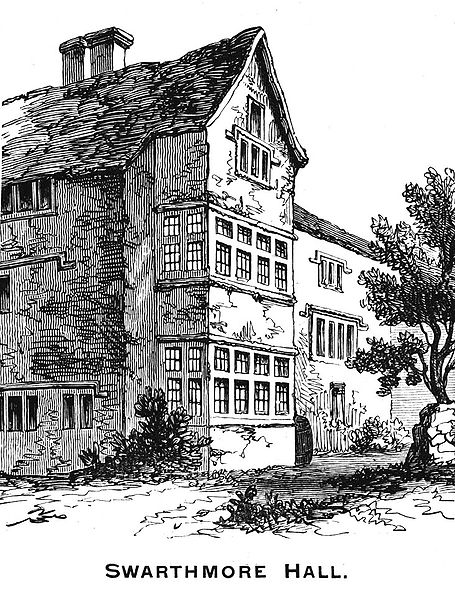
\includegraphics[width=0.20\textwidth]{./pics/swarthmore_hall.png}
\label{bild:swarthmoor} 
\end{floatingfigure}

\section{Kampf gegen Verleumdung}

Wir zogen durch Nottinghamshire\ort{Nottinghamshire} 
nach Lincolnshire\ort{Lincolnshire} [...].
Hier kam zu einer unserer Versammlungen ein Mann und erhob eine
falsche Anklage gegen mich; er verbreitete 
überall das Gerücht\index{Gerücht}, ich
habe gesagt, ich sei Christus, was gänzlich falsch war. Als ich dann
nach Gainsborough\ort{Gainsborough} kam, wo einer 
der Freunde auf dem Marktplatz die Wahrheit 
verkündet hatte, fand ich die ganze Stadt und
alle Marktleute in Aufruhr. Ich ging ins Haus eines Freundes,
und das Volk drängte sich hinter mir drein, bis das Haus ganz
voll war von \textit{Frommen}, Eiferern und Pöbel; da kam jener
falsche Verleumder herein und klagte mich öffentlich vor allen an,
ich hätte gesagt, ich sei Christus, und er habe Zeugen, es zu 
beweisen. Das brachte die Leute so in Wut, das man Mühe hatte,
mich vor ihnen zu schützen. Da trieb mich der Geist des Herrn
aus einen Tisch zu stehen und in der ewigen Kraft des Herrn
den Leuten zu verkünden, das Christus in ihnen sei, es sei denn,
das sie Verdammte seien; und das es Christus, die ewige Kraft
Gottes sei, welche jetzt aus mir zu ihnen rede, nicht ich sei Christus;
die Leute waren im allgemeinen befriedigt außer jenem \textit{Frommen}
und einigen falschen Zeugen. Ich nannte diesen Ankläger
Judas\index{Beleidigung}\index{Judas}\person{Fox!verbaler Angriff},
und es trieb mich, ihm zu sagen, das das Ende des Judas auch
das seine sein werde; solches lasse ihm der Herr durch mich sagen.


Des Herrn Macht kam über alle und beruhigte die Gemüter der
Leute und sie gingen in Frieden fort. Jener Judas aber machte
sich davon und erhängte sich und man steckte einen Pfahl in sein
Grab. Daraufhin erhoben die bösen 
Priester eine Verleumdung\index{Verleumdung}
gegen uns und streuten aus, ein Quäker habe sich erhängt in
Lineolnshire. Diese Lüge ließen sie drucken und verbreiten und
häuften so Sünde auf Sünde. Aber wir und die Wahrheit wurden
nicht davon getroffen; denn jener war so wenig ein Quäker als
der Priester, der solches gedruckt hatte; vielmehr war es einer
% \picinclude{./050-059/p_s057.jpg} 
ihrer eigenen Leute. Aber trotz dieser argen Lüge, mit welcher der
Gegner beabsichtigt hatte, uns zu verleumden und die Leute von
der von uns verkündeten Wahrheit abzukehren, nahmen doch viele
in Lincolnshire das Evangelium an, da sie von der ewigen 
Wahrheit überzeugt waren und sich zu Füßen des himmlischen Herrn
setzten [...].

\section{Schwere Misshandlung von Fox und Freunden}

Wir zogen nun wieder [...] über Warmsworth [...] Bably,
Doncaster [...] nach Tikhill, wo an einem Ersten Tage die
Freunde der Gegend sich versammelten, und es herrschte durch
Gottes Macht eine tiefe Zerknirschung in der Versammlung.
Ich verließ die Versammlung, da Gott mich trieb ins Turmhaus
zu gehen. Als ich dorthin kam, fand ich den Priester und fast
alle Gemeindeältesten im Chor beisammen. Ich ging zu ihnen
und hub an zu ihnen zu reden, aber sie fielen sogleich über mich
her, und ein Priester nahm seine Bibel und schlug mich damit
ins Gesicht, so das ich heftig blutete im Turmhaus; das Volk
schrie: \zitat{Hinaus mit ihm aus der Kirche!} Und als sie mich hinaus
gebracht hatten, prügelten sie mich und warfen mich zu Boden
und über eine Hecke; hernach schleppten sie mich durch ein Haus
auf die Straße; sie bewarfen mich mit Steinen und schlugen mich,
während sie mich Vorwärts rissen, so das ich über und über mit
Kot beschmiert war. Sie nahmen mir den Hut, den ich nicht
mehr wieder bekam. 

Als ich jedoch wieder auf den Füßen war,
verkündete ich ihnen das Wort des Lebens und zeigte ihnen, 
wohin ihre Lehre sie führe und wie sie das Christentum entehrten. Nach
einer Weile ging ich wieder in die Versammlung zurück zu den
Freunden. Und als die Priester und die Leute am Hause vorbei
kamen, ging ich mit einigen Freunden hinaus in den Hof und
redete zum Priester und den Leuten. Der Priester verhöhnte
uns und nannte uns \zitat{Quäker}. Aber die Macht des Herrn
kam dermaßen über sie und das Wort des Lebens wurde ihnen
so überzeugend und eindringlich verkündet, das der Priester selber
zu zittern\index{zittern} begann und einer 
sagte: \zitat{seht wie der Priester zittert
und bebt, er wird auch ein Quäker}. Als die Versammlung zu
Ende war, gingen die Freunde fort, und ich ging, ohne Hut,
nach Balby, etwa sieben bis acht Meilen weit. 

Die Freunde
wurden an dem Tage dergestalt von dem Priester und seinen
Anhängern misshandelt, das einige Friedensrichter, als sie davon
hörten, kamen und ein Verhör in dieser Stadt anstellten, um
% \picinclude{./050-059/p_s058.jpg} 
die Sache zu untersuchen. Der, welcher mich blutig geschlagen
hatte, fürchtete, man haue ihm die Hand ab; aber ich vergab
ihm und klagte nicht gegen ihn.

\section{Verhaftung von Thomas Aldam}

Zu Anfang des Jahres 1652\jahr{1652} regte sich heftiger Widerstand
gegen die Wahrheit und die Freunde, bei Priestern und Volk
und bei etlichen der Behörden in Yorkshire\ort{Yorkshire}, 
so das der Priester
von Warmsworth sich einen Verhaftbefehl gegen mich und Thomas
Aldam\person{Aldam, Thomas} verschaffte, der in allen 
Teilen im westlichen Bezirk Yorkshires ausgeführt 
werden konnte. Zu dieser Zeit hatte ich ein
Gesicht\index{Vision} von einem Bären und zwei großen, 
riesigen Hunden, und
wie ich bei ihnen vorbei musste, ohne das sie mir etwas tun
konnten. Und so geschah es; denn der Konstabler ergriff Thomas
Aldam und brachte ihn nach York\ort{York}; und ich ging 
ein großes Stück
Wegs mit ihm. Der Kanstabler hatte auch einen Verhaftbesehl
gegen mich und sagte zu mir: er sehe mich schon, aber er möge
nicht einen der ihm fremd sei, behelligen; Thomas Aldam sei
eben sein Nachbar. Also hielt ihn die Kraft des Herrn, das er
mich in Ruhe lies. 

Wir kamen in die Wohnung des Leutnant 
Roper\person{Leutnant Roper}, wo wir eine 
große Versammlung hatten, worunter viele
angesehene Leute waren; die Wahrheit wurde mächtig kund
unter ihnen und die Schrift herrlich erklärt, und die Gleichnisse
und Reden Jesu wurden ausgelegt und die Kirche, wie sie in den
Tagen der Apostel war, und der Abfall von derselben. Die
Wahrheit gelangte zur Herrschaft an jenem Tage, so das jene
angesehenen Leute alle zugestanden: \zitat{diese Anschauungen werden
sich über die ganze Erde ausbreiten}. Dieser Versammlung
wohnten auch James Naylor\person{Naylor, James}, 
Thomas Goodyear\person{Goodyear, Thomas} und 
William Dewsbury\person{Dewsbury, William}, die das 
Jahr vorher gewonnen worden waren, sowie
Richard Farnsworth\person{Farnsworth, Richard} bei. Der 
Konstabler blieb mit Thomas
Aldam, bis die Versammlung aus war, dann ging er mit ihm
nach dem Gefängnis in York; mich aber lies er in Ruhe [...].

\section{Pendlehill}

Darnach kam ich nach Hightown\ort{Hightown}, wo eine 
Frau wohnte, die
kurz vorher bekehrt worden war. Wir gingen in ihr Haus und.
hielten eine Versammlung, und die Leute versammelten sich, und
wir verkündeten ihnen die Wahrheit und wirkten für den Herrn
unter ihnen, und sie gingen in Frieden wieder von dannen.
Aber es war dort eine Witwe, namens 
Green\person{Green, Witwe}, von böser Gesinnung; 
diese ging zu einem sogenannten \textit{Ehrenmann} (Gentleman)
und verklagte uns bei ihm, obwohl er kein Beamter war. Am
% \picinclude{./050-059/p_s059.jpg} 
nächsten Morgen sandten wir dem Priester einige Fragen. Als
wir gerade fort gehen wollten, kamen einige, die sich zu uns
hielten, gerannt und sagten, dieser Mörder habe sein Schwert
für uns geschärft und komme mit demselben gegen uns. Da wir
gerade fort gingen, verfehlten wir ihn. Aber kaum waren wir
fort, so kam er in das Haus, in dem wir gewesen waren, und
es hieß allgemein, wenn wir nicht fort gewesen wären, so wären
wir ermordet worden. Wir brachten die Nacht im Walde zu
und wurden ganz durchnässt, denn es regnete stark. Am Morgen
trieb es mich wieder in die Stadt zurück, wo sie uns ausführlich
über jenen Bösewicht berichteten.


Von da gingen wir nach Bradford\ort{Bradford}, wo wir 
Richard Farnsworth trafen, von dem wir uns kurz vorher getrennt hatten.
Als wir in sein Haus kamen, setzte man uns Fleisch vor, aber als
ich anfangen wollte, geschah das Wort des Herrn 
an mich:\person{Fox!Eingebung} 
\zitat{Iss nicht Brot bei einem Neidischen} 
(Spr.~23:6\bibel{Spr. 23:06@Spr. 23:6}). Sogleich stand ich
vom Tische auf und aß nichts. Die Frau war eine 
Baptistin\index{Baptististen}.
Nachdem ich die ganze Familie ermahnt hatte, sich zum Herrn
zu bekehren und auf seine Lehre in ihren Herzen zu merken,
gingen wir von dannen [...].

Unterwegs kamen wir zu einem großen Hügel, genannt 
Pendlehill\ort{Pendlehill}; und der Herr trieb mich, 
auf denselben hinauf zu gehen,
was ich mit großer Anstrengung tat, denn er war sehr steil und
hoch. Als ich oben ankam, blickte ich auf das Meer, das 
Lancashire\ort{Lancashire} umspült. Von diesem Hügel aus 
zeigte mir der Herr
die Orte, wo ihm ein großes Volk sollte gesammelt werden.
Beim Hinuntergehen fand ich eine Wasserquelle am Abhang
des Hügels, aus der ich mich erfrischte, denn ich hatte in den
letzten Tagen nur wenig gegessen und getrunken. Am Abend
kamen wir zu einer Herberge [...] und hier lies mich der
Herr ein Vision\index{Vision} sehen: eine große Schar 
in weisen Kleidern
am Ufer eines Flusses, die zum Herrn kamen, und der Ort, den
ich sah, war bei Wensleydale und Sedbergh [...].

Wir zogen durch die Dales [...] nach Dent [...]. Hier ging
ich zu Richard Robinson und redete von der Wahrheit zu ihm:
In einer Versammlung bei Friedensrichter 
Benson\person{Benson, Friedensrichter} traf ich Leute,
die sich vom öffentlichen 
Gottesdienst\index{Gottesdienst!öffentlicher} losgesagt hatten. Dies
war der Ort, den ich gesehen, wo eine Schar in weisen Kleidern
daher kam. Es war eine große Versammlung, und die meisten
% \picinclude{./060-069/p_s060.jpg} 
wurden gewonnen und haben noch jetzt große Versammlungen von
Freunden in der Nähe von Sedbergh, die ich damals zuerst 
zusammen sammelte im Namen Jesu.


Es fand ein großer Jahrmarkt statt, an welchem man pflegte
Dienstboten zu dingen; ich verkündete den Tag 
des Herrn\index{Tag des Herrn}. Nach 
dem ich dies getan, ging ich auf den Platz des Turmhausets, und
viele Leute kamen vom Jahrmarkt zu mir und eine Menge Priester
und \textit{Fromme}. Da verkündete ich die 
ewige Wahrheit\index{Wahrheit!ewige} des
Herrn und das Wort des Lebens während 
mehrerer Stunden\person{Fox!stundenlang predigen}
und zeigte, das der Herr gekommen sei, sein Volk selbst zu lehren
und es abzubringen von den Wegen dieser Welt und ihren Lehrern,
zu Christus dem wahren Lehrer und wahren Weg. Ich machte
ihnen klar, wie ihre Lehrer denen gleich seien, die von jeher
von den Propheten, von Christus und den Aposteln verdammt.
worden sind. Ich ermahnte alle von ihren mit Händen gemachten
Tempeln abzulassen und auf den Empfang des Geistes zu warten,
damit sie erkennen könnten, das sie der Tempel Gottes seien.
Nicht ein einziger von den Priestern hatte Macht, seinen Mund
aufzutun gegen das, was ich verkündete; zuletzt sagte einer von
der Wache: \zitat{Warum geht ihr nicht in die Kirche? hier ist
kein geeigneter Platz zum Predigen}.\index{Predigen!richtiger 
Ort} Ich sagte ihm, ich leugne
ihre Kirche. Da erhob sich Francis 
Howgill\person{Howgill, Francis}\footnote{Francis Howgill, 
später ein eifriger Qnäkerprediger (s.Weingarten a.a.D.)}, 
Prediger einer
Gemeinschaft. Er hatte mich nie vorher gesehen, aber er unternahm
es, diesem Hauptmann zu antworten und brachte ihn bald zum
Schweigen; und von mir sagte er: \zitat{dieser predigt gewaltig und
nicht wie die Schriftgelehrten 
(Matth.~7:29\bibel{Matth. 07:29@Matth. 7:29})}. Ich erklärte 
darauf den Leuten, das dieser Boden hier nicht heiliger sei als an
einem andern Ort und das nicht dieses Haus die Kirche sei,
sondern die Gemeinde, deren Haupt Christus ist. Bald nachher
kamen dann einige Priester zu mir und ich ermahnte sie, Buße zu
tun. Einer von ihnen sagte, ich sei 
verrückt\person{Fox!für verrückt gehalten}, und wandte sich von
mir ab; aber manche wurden gewonnen an dem Tage und freuten
sich über die Verkündigung der Wahrheit und nahmen sie mit
Freuden auf. Einer unter ihnen, Hauptmann Ward, nahm die
Wahrheit in Liebe auf und lebte darin bis zu seinem Tode [...].

\section{Unterbarrow}

Von da ging ich nach Unterbarrow, zu einem namens Miles
Bateman\person{Bateman, Miles} [...]. Am Morgen ging ich 
aus [...] und als ich in
% \picinclude{./060-069/p_s061.jpg} 
der Nähe auf einem Hügel hin und her ging, sah ich einige
Reisende, welche um Unterstützung baten, und ich sah, das sie
es nötig hatten; aber man gab ihnen nichts und sagte ihnen, sie
seien Strolche. Es betrübte mich solche Hartherzigkeit unter den
\textit{Frommen} zu sehen, und als sie alle beim Frühstück saßen, lief
ich den Reisenden etwa eine viertel Meile nach und gab ihnen
etwas Geld\person{Fox!Geldspende}. Als nun einige von den andern 
aus dem Hause
kamen und sahen, das ich eine viertel Meile weg war, sagten sie, ich
hätte nicht so weit kommen können, wenn ich nicht Flügel hätte.
Daraufhin war es nahe daran, das man die Versammlung 
absagte; denn man hatte eine so merkwürdige Meinung von mir
bekommen, das viele nicht eine Versammlung mit mir haben
wollten\person{Fox!wundersamer Eindruck}. Ich 
sagte ihnen, ich sei jenen armen Reisenden  
nachgelaufen, um ihnen etwas Geld zu geben, weil mich die 
Hartherzigkeit, mit der man sie fortgeschickt, betrübt habe [...].

\section{Swarthmore}

Von da ging ich nach Ulverstone\ort{Ulverstone} 
und Swarthmore\ort{Swarthmore} zu
Richter Fell\person{Fell, Richter}; es kam auch einer, 
Priester Lampitt\person{Lampitt, Priester}, der behauptete,
Eingebungen\index{Eingebungen} zu haben Ich redete 
lange mit ihm, denn er sprach
von wichtigen Eingebungen und von 
Vollkommenheit\index{Vollkommenheit} und 
blendete die Leute dadurch. Er hätte mich gerne gewähren lassen,
aber ich konnte ihn nicht gewähren lassen, weil er so unlauter
war. Er sagte, er sei mehr als Johannes, und tat, als ob er
alle Dinge wüste. Ich sagte ihm, der Tod habe von Adam bis
Moses regiert (Röm. 5:14\bibel{Röm. 05:14@Röm. 5:14}); 
und weil er tot sei, kenne er Moses
nicht, denn Moses habe das Paradies Gottes gesehen; er aber
kenne weder Moses noch die Propheten noch Johannes. Denn
die höckerichte\footnote{Unklar was gemeint ist} 
und raue Natur war noch in ihm, und der Berg
der Sünde und des Verderbens, und der Weg für den Herrn
war nicht bereitet in ihm (Jes. 40\bibel{Jes. 40}). 
Er bekannte, er sei in großer
Trübsal gewesen, beteuerte aber, nun könne er Psalmen singen
und alles machen, was; man von ihm verlange. Ich sagte ihm,
er gehöre zum Diebesgesindel, aber Moses und die Propheten
und Christus predigen, das könne er nicht; dazu müsste er den
gleichen Geist haben wie jene. 

Margaret 
Fell\person{Fell, Margaret} war den ganzen
Tag nicht zu Hause gewesen; am Abend erzählten ihr ihre Kinder,
das Priester Lampitt und ich gestritten hätten; dies betrübte sie,
weil er dem gleichen Bekenntnis angehörte wie sie; aber er
verbarg sein schmutziges Treiben vor ihnen.
Wir sprachen noch lange miteinander am Abend, und ich verkündete
% \picinclude{./060-069/p_s062.jpg} 
ihr und ihrer Familie die Wahrheit. Am folgenden Tage
kam Lampitt wieder, und ich redete lange mit ihm, und Margaret
Fell, die ihn jetzt ganz durchschaute, war dabei. Eine 
Überzeugung der Wahrheit kam über sie und die Ihrigen. Als bald
darauf ein allgemeiner Bustag\index{Bustag} abgehalten 
werden sollte, bat sie
mich, mit ihr ins Turmhaus von Ulverstone\ort{Ulverstone} 
zu kommen, denn
sie hatte sich noch nicht gänzlich davon losgemacht. Ich erwiderte
ihr: \zitat{Ich muss tun, wie mich der Herr heißt.} Ich verließ sie
und ging ins Freie und das Wort des Herrn geschah also zu
mir: \zitat{Gehe ihnen nach ins Turmhaus}\person{Fox!Eingebung} 


Als ich kam, sang
Lampitt gerade mit den Leuten; aber sein Geist war so unlauter,
und was sie sangen\index{Gesang}, passte so wenig 
für ihr Bedürfnis, das, als
sie fertig gesungen hatten, der Herr mich trieb, also zu ihnen zu
reden: \zitat{Der ist nicht ein Jude\index{Jude}, der es 
äußerlich ist, sondern der
ist ein Jude, der innerlich einer ist, in seinem Leben, das er nicht
vor den Menschen, sondern vor Gott führt} 
(Röm. 2:28+29\bibel{Röm. 02:28+29@Röm. 2:28+29}).
Dann zeigte ich ihnen nach des Herrn weiterer Offenbarung, das
Gott gekommen sei, sein Volk zu lehren 
(1.Joh. 2:27\bibel{Joh. 1. 02:27@1.Joh. 2:27}), 
(Joh. 14:26\bibel{Joh. 14:26}).
durch seinen Geist und sie abzubringen von allen ihren früheren
Gebräuchen, ihren Bekenntnissen, Kirchen und Gottesdiensten;
denn das alles seien nur Menschensatzungen; das Leben und den
Geist, auf dem diese Satzungen entstanden, die hätten sie doch
nicht. 

Da rief Friedensrichter Sawrey\person{Sawrey, Friedensrichter}: 
\zitat{Fort mit ihm!} Aber
Richter Fells Frau\person{Fell, Margaret} sagte zu den 
Beamten: \zitat{Last ihn gehen;
warum soll er nicht so gut reden wie ein anderer?} Auch Lampitt,
der Betrüger, sagte, man solle mich reden lassen. Aber als ich eine
Zeit lang geredet hatte, lies mich Friedensrichter Sawrey hinaus
bringen durch die Konstabler; da redete ich auf dem Kirchhof
weiter [...]\person{Fox!Rauswurf}. Ich ging nun nach 
Becliff\ort{Becliff} [...] und andere Orte [...].


Bald darauf, als Richter Fell nach Hause kam, lies Margaret
Fell mich holen und lies mir sagen, ich solle doch zu ihnen
kommen; ich fühlte die Freiheit vom Herrn, es zu tun und ging
hin. Ich sah, das die Priester und die \textit{Frommen} und der
Friedensrichter Sawrey, Richter Fell und Hauptmann Sande durch
ihre Lügen gegen die Wahrheit eingenommen hatten, aber als ich
kam und mit ihnen redete, gelang es mir, alle ihre Einwände zu
widerlegen, und ich überzeugte Hauptmann Sands an Hand der
Schrift so völlig, das er ganz befestigt war in seiner Überzeugung.
Nach einigem Hin und Her reden war Richter Fell ebenfalls 
% \picinclude{./060-069/p_s063.jpg} 
zufrieden gestellt und gelangte dazu, durch das, was ihm der Geist
Gottes eröffnet hatte, etwas Höheres zu erkennen, als was die
weltlichen Priester und Lehrer lehrten, und ging nicht mehr hin,
sie zu hören alle die Jahre bis zu seinem Tode; denn er wusste
nun, das das, was ich lehrte, die Wahrheit sei, und das Christus
der Lehrer seines Volkes ist und sein Heiland [..]. 

Während ich
in dieser Gegend war, kamen Richard 
Farnsworth\person{Farnsworth, Richard} und James
Naylor\person{Naylor, James}, mich und die anderen 
zu sehen, und weil Richter Fell
nun darüber beruhigt war, das es die Wahrheit sei, die ich ver-
kündige, so erlaubte er mir, Versammlungen in seinem Hause zu
haben trotz aller Einwände; und es wurde eine große Versammlung 
eingerichtet, die fast vierzig Jahre, bis 
1690\jahr{1690}, bestand, so
das ein neues Versammlungshaus\index{Versammlungshaus} 
in der Nähe gebaut wurde [...].

Ich hörte von einer großen Versammlung, die in Ulverstone
stattfinden sollte, und ging darum dorthin und begab mich ins
Turmhaus, in der Furcht und der Kraft Gottes. Als der Priester
geendet hatte, redete ich das Wort des Herrn zu ihnen, das wie ein
Hammer und ein Feuer unter ihnen wirkte 
(Jer. 23:29\bibel{Jer. 23:29}). Lampitt,
der Priester des Ortes, war mit den meisten andern Priestern
uneins gewesen vorher, nun aber taten sie sich alle zusammen
gegen die Wahrheit. Aber die mächtige Kraft des Herrn war
über allem und tat sich so herrlich kund, das Priester Bennett
sagte: \zitat{Die Kirche erbebt!} und sich 
fürchtete und zitterte\index{zittern}. Und
nachdem er einige unverständliche Worte geredet, eilte er hinaus,
aus Furcht, sie möchte über seinem Kopf zusammenstürzen. Viele
Priester versammelten sich, aber sie hatten noch keine Macht, 
Verfolgungen zu veranstalten.

\section{Fox über Berufung und Erfahrung}

Als ich nun hier fertig war, ging ich wieder nach 
Swarthmore, wohin vier oder fünf Priester kamen; im Gespräch mit
ihnen fragte ich, ob einer unter ihnen sei, der sagen könne, das
Wort des Herrn: \zitat{Gehe hin und rede zu den oder jenen}, sei je
einmal an ihn ergangen?\index{Berufung} Keiner wagte, es von sich zu 
behaupten. Aber einer von ihnen wurde zornig und sagte, er
könne von Erfahrungen so gut berichten wie ich. Ich erwiderte
ihm, Erfahrungen seien allerdings etwas, aber eine Botschaft
erhalten und damit ausziehen, ein Wort vom Herrn haben und
verkünden wie die Apostel und Propheten und wie ich, wenn
ich unter ihnen predige, das sei noch etwas anderes. Und ich
fragte sie darum noch einmal, ob einer unter ihnen sagen könne,
% \picinclude{./060-069/p_s064.jpg} 
er habe irgend einmal einen Befehl unmittelbar vom Herrn
empfangen; aber es konnte es keiner. Da erklärte ich ihnen, das
seien falsche Propheten und falsche 
Apostel und Antichristen\index{Antichrist} die
die Worte der wahren Propheten und wahren Apostel und Christi
gebrauchen und die Erfahrungen anderer verwenden und selber
nie eine Stimme Gottes oder Christi vernommen haben. Solche
wie sie könnten eben bloß die Erfahrungen und Worte anderer
vernehmen. Das verwirrte sie sehr und stellte sie bloß. Ein
andermal im Gespräch mit einigen Priestern im Hause Richter
Fells und in dessen Anwesenheit stellte ich die gleiche Frage und
fügte hinzu: das könne eben jeder, der lesen könne, die 
Erfahrungen der Propheten und Apostel verkünden, die in der Schrift
aufgezeichnet seien. Hierauf bekannte ein alter Priester, Thomas
Taylor\person{Taylor, Thomas}, dem Richter Fell ehrlich: 
er habe nie die Stimme Gottes
oder Christi\index{Offenbarung} vernommen, die ihn 
irgendwohin gesandt habe; er
rede von seinen eigenen Erfahrungen und den Erfahrungen der
Heiligen früherer Zeiten, und dies predige er. Solches bestärkte
Richter Fell in der Überzeugung, das die Priester im Irrtum
seien. Denn er hatte vorher, wie die meisten Leute damals,
geglaubt, sie seien von Gott gesandt.

Zu dieser Zeit wurde Thomas Taylor\footnote{Thomar Taylor 
hatte in Oxford studiert und war Puritanerprediget\index{Puritaner}
geworden. Dann, weil er nicht mehr wollte 
\zitat{für Lohn predigen}, schloss er sich den Quakern an 
und wirkte eifrig als Prediger und durch Schriften.} bekehrt und 
durchreiste mit mir Westmorland\ort{Westmorland} [...]. 
Die Priester wurden immer
aufgebrachter gegen uns und verfolgten uns, wo sie nur konnten.
James Naylor\person{Naylor, James} und Francis 
Howgill\person{Howgill, Francis} wurden ins Gefängnis 
geworfen [...]. Aber dem Herrn sei Lob, die Wahrheit breitete sich
immer mehr aus. Denn um diese Zeit spürten sich 
John Audland\person{Audland, John}, John 
Camm\person{Camm, John}, Edward 
Burrough\footnote{Edward Burtough, ursprünglich 
Prediger der Epiekopalkirche\index{Epiekopalkirche}, war
aus dieser ausgetreten und hatte sich den Präsbyterianern 
angeschlossen; nach einigen Unterredungen mit Fox bekehrte 
er sich sodann zum Quäkertnm, dessen eifriges tätiges Glied er 
blieb, bis er 1662\jahr{1662} für seinen Glauben im Kerker, wohin
man ihn aus einer Versammlung gebracht hatte, starb.}, 
Richard Hubberthorn\person{Hubberthorn, Richard} eine 
bescheidene, friedliche Natur, kränklich und
mit einer schwachen Stimme, arbeitete dennoch Großes als 
Prediger. 1662\jahr{1662} wurde er ebenfalls aus einer 
Versammlung in den Kerker geschleppt, wo sein schwacher
Körper bald den Entbehrungen erlag; doch pries er noch 
auf seinem Totenbett die Güte Gottes.
% \picinclude{./060-069/p_s065.jpg} 
und andere mit der Kraft von oben ausgerüstet und traten auf
als Prediger und erwiesen sich als treue Arbeiter, die umher
zogen und das Evangelium umsonst predigten, wodurch Tausende
bekehrt wurden und von nun an dem Herrn gehörten [...].

\section{Priester Lampitt lässt Fox und seine Freunde scher misshandeln}

Nachdem ich die Freunde in Westmorland besucht hatte, ging
ich wieder nach Uloerstone, wo Priester 
Lampitt\person{Lampitt, Priester} war. Dieser
hatte selber gepredigt, man müsse sich von Gott lehren lassen;
und alle Menschen, Männer und Frauen, können dazu kommen,
das Evangelium zu predigen. Als es sich aber darum handelte,
dies mit der Tat zu beweisen, so verfolgte er sowohl diese Lehre
als die Lehrer [...]. Als nun die Versammlungen ihren Anfang
nahmen und wir in einer Privatwohnung zusammen kamen, wurde
Lampitt sehr aufgebracht und sagte, wir verlassen den Tempel
und gehen in den Götzentempel Jerobeams, so das viele der
\textit{Frommen} sahen, wie wenig er mit dem, was er gepredigt hatte,
Ernst machte. Nun legte man ihnen die Sache mit dem 
Götzentempel Jerobeams 
(1. Könige 13\bibel{Könige 1. 13@1. Könige 13}), aus 
und zeigte ihnen, das
eher ihre Häuser, die sie Kirchen nennen, die Götzentempel 
Jerobeams seien und die alten Meßhäuser, die das 
finstere Papsttum\index{Papsttum}
eingesetzt und die jene, die sich 
Protestanten\index{Protestanten} nennen und meinen,
sie seien aufgeklärter als die Päpstlichen, auch noch festhalten,
obgleich doch Gott sie nie angeordnet. Und der 
Tempel\index{Tempel}, den
Gott in Jerusalem eingesetzt, dem habe Christus. eine Ende 
gemacht, und die, welche ihn aufnahmen und an ihn glaubten, deren
Leiber wurden Tempel Gottes, in denen Christus und der heilige
Geist wohnen (1. Cor. 6:19\bibel{Cor. 1. 6:19@1. Cor. 6:19}) 
Diese versammelten sich [...]
und kamen zusammen in ihren Wohnhäusern, die dann nicht
Tempel genannt wurden oder Kirchen, sondern ihre Leiber waren
die Tempel und die Gläubigen die Kirche, deren Haupt Christuts
ist [...]. 

Darauf trieb es mich ins Turmhaus zu gehen, wo Priester
und \textit{Fromme} und viel Volk versammelt waren. Ich stand in der
Nähe von Priester Lampitt, der darauf los wütete in seiner
Predigt. Nachdem der Herr meinen Mund aufgetan, das ich
reden sollte, kam Friedensrichter John 
Sawrey\person{Sawrey, Friedensrichter John} zu mir und sagte,
wenn ich mich an das halten wolle, was in der Schrift stehe,
so könne ich reden.\index{bibeltreu} Ich wunderte mich über 
diese Rede und sagte,
ich werde mich sicher an die Schrift halten und sie vorweisen,
um das Gesagte zu begründen; denn ich hätte ihm und Lampitt
etwas zu sagen. Hierauf sagte er wieder, ich solle nicht reden,
George Fox. 
% \picinclude{./060-069/p_s066.jpg} 
und widersprach sich damit selber, nachdem er ja eben gesagt
hatte, ich solle reden, wenn ich mich an die Schrift halten wolle.
Die Leute waren ruhig und hörten mir gerne zu, bis 
Friedenstichtet Sawrey, der Hauptanstifter der grausamen Verfolgung
im Norden, sie gegen mich aufhetzte, und sie anfingen, mich zu
stoßen, schlagen und quälen. Sie gerieten alsbald in Wut und
fielen über mich her, im Turmhaus, und schlugen mich vor seinen
Augen zu Boden, stießen mich und traten mich mit 
Füßen.\person{Fox!Misshandlung} Der
Aufruhr war groß, so das etliche über ihre Stühle fielen im
Gedränge. Schließlich kam Sawrey und befreite mich aus ihren
Händen und führte mich hinaus und übergab mich den Konstablern
und hieß sie mich peitschen und zur Stadt hinaus führen. Sie
führten mich etwa eine Meile weit, etliche hielten mich am Kragen,
etliche an den Armen und den Schultern und schleppten und
zerrten mich vorwärts. Von den Freunden, die auf den Markt
und ins Turmhaus gekommen waren, um mich zu hören, wurden
viele auch zu Boden geworfen und dermaßen geschlagen, das
manche von Blut überströmt waren. Richter Fells Sohn, der
mir nachrannte, um zu sehen, maß mit Mir geschehe, warfen sie
in einen Wassergraben und einige schrien: \zitat{schlagt ihm die Zähne
aus dem Kopf.} Als sie mich nun bis ins Moor hinausgeschleppt
hatten, gefolgt von einem großen Haufen, gaben mir die 
Konstabler mit ihren Weidenruten ein paar Schläge über den
Rücken und überließen mich dem Pöbel, der mit Stöcken, 
Heckenpfählen, Stechpalmen und Eichenzweigen versehen über mich
herfiel und mich auf Kopf und Glieder schlug, bis mir die
Sinne vergingen und ich auf den nassen Boden hinfiel. 


Als ich wieder zu mir kam und merkte, das ich aus der nassen
Erde lag und die Leute mich umstanden, blieb ich einige
Zeit unbeweglich; und die Kraft des Herrn durchzuckte mich und
die ewige Erquickung erquickte mich, so das ich wieder aufstehen
konnte in der stärkenden Kraft des Herrn; und die Arme 
ausstreckend, sagte ich mit lauter Stimme: \zitat{Schlaget wieder, 
hier sind meine Arme, mein Kopf und meine Wangen.} Einer aus
dem Haufen, ein \textit{Frommer}, aber ein roher Kerl, schlug mir
mit seinem Stab gerade auf die ausgestreckte Hand; meine Hand
wurde von diesem Schlag so zerquetscht und mein Arm so 
gelähmt, das ich ihn nicht wieder zurück ziehen konnte, und etliche
riefen: \zitat{Seine Hand ist für immer verstümmelt; er wird sie nie
% \picinclude{./060-069/p_s067.jpg} 
mehr gebrauchen können!} Aber ich betrachtete die Hand in der
Liebe zu Gott; denn ich stand zu allen, die mich verfolgt hatten,
in der Liebe Gottes; und nach einer Weile durchzuckte mich die
Liebe Gottes und zuckte durch meinen Arm und meine Hand,
so das ich augenblicklich die Kraft darin wieder spürte, vor aller
Augen.\person{Fox!Wunderheilung} Daraufhin gerieten sie 
selber untereinander in Streit und
sagten mir, wenn ich ihnen Geld gebe, so wollten sie mich vor
den andern schützen. Aber der Herr trieb mich, ihnen das Wort
des Lebens zu verkünden, und ich zeigte ihnen, was sie für ein
verkehrtes Christentum haben, und was für Früchte die Predigten
ihrer Priester brächten; ich sagte ihnen, sie seien 
eher Juden\index{Juden} oder Heiden\index{Heiden} als Christen. 


Darauf trieb mich der Herr, wieder durch
das Volk hindurch auf den Markt von Ulverstone zu gehen. Auf
dem Wege begegnete mir ein Soldat\index{Soldat} mit dem Schwert an der
Seite: \zitat{Herr,} sagte er, \zitat{ich sehe, das Ihr ein 
Mann seid, und es tut mir Leid, das Ihr so misshandelt werdet;}
und er bot mir
an, mir nach Kräften zu helfen. Aber ich sagte ihm: 
\zitat{Die Kraft des Herrn ist über Alles,} und ging 
durch das Volk hindurch auf
den Markt, und keiner hatte Macht, mich anzurühren. 

Und als
auf dem Markte einige Freunde misshandelt wurden, und ich jenen
Soldaten mit seinem 
nackten Schwerte\index{Schwerte}\index{Selbstverteidigung} 
mitten darunter sah, da
sprang ich hinzu, ergriff seinen Arm und befahl ihm, das Schwert
wieder einzustecken, wenn er es mit mir halten wolle, und mit
mir aus dem Haufen heraus zu kommen; denn ich wolle nicht,
das durch ihn ein Unheil geschehe. 

Einige Tage darauf wurde
dieser Soldat von sieben Männern ergriffen und durchgeprügelt,
weil er es mit mir und den Freunden gehalten habe. Es war
in jenen Tagen die Art der Verfolger in diesen Gegenden,
ihrer 20 oder 40 auf einen einzigen loszugehen. An Vielen Orten
wurden die Freunde in der Weise überfallen, das sie schier nicht
auf die Straße konnten; man warf ihnen Steine an und 
misshandelte sie. 

Als ich nach Swarthmore kam, kam ich gerade
dazu, wie die dortigen Freunde den Freunden die von Lampitts
Zuhörern misshandelt worden waren die gebrochenen und 
verletzten Glieder verbunden. Mein ganzer Körper war gelb, schwarz
und blau von den Schlägen, die ich an jenem Tage erhalten
hatte. Und die Priester fingen wieder an zu prophezeihen, das
wir in einem halben Jahr alle vernichtet sein würden.

\section{Insel Walney}

Etwa zwei Wochen später ging ich auf die 
Insel Walney\ort{Insel Walney} und
% \picinclude{./060-069/p_s068.jpg} 
James Naylor\person{Naylor, Jame} mit mir. An einem Morgen 
ging ich mit einem
Boot zu James Lancaster\person{Lancaster, James}. Sowie 
ich ans Land stieg, stürzten vierzig
Männer mit Stöcken, Fischangeln und Knütteln hervor, überfielen
mich, schlugen und zerrten mich und versuchten, mich ins Wasser zurück
zu stoßen.\index{Misshandlung} Als sie mich beinahe in die 
See zurück geworfen hatten
und ich sah, das sie mich umbringen wollten, lief ich mitten unter sie
zurück; aber sie fielen wieder über mich her und schlugen mich,
bis ich betäubt war. Als ich wieder zu mir kam, sah ich wie
James Lancasters Frau Steine nach meinem Gesicht warf, und
ihr Mann beugte sich über mich, um die Steine von mir 
abzuhalten. Die Leute hatten James Lancasters Frau glauben
machen, ich hätte ihren Mann verhext, und hatten ihr 
versprochen, wenn sie ihnen melde, wann ich kommen werde, so
wollten sie mich töten. Und als bekannt wurde, das ich komme,
hatten viele aus der Stadt sich aufgemacht, mit Knütteln und
Stöcken, um mich zu töten. Aber die Kraft des Herrn
schützte mich, das sie mir nichts antun konnten. Zuletzt gelang
es mir, wieder aufzustehen; aber sie warfen mich sogleich wieder
ins Boot zurück. Als James Lancaster es sah, kam er sogleich
und brachte mich übers Wasser, das ich vor ihnen sicher war;
aber so lange wir noch erreichbar waren auf dem Wasser, warfen
sie uns Steine nach. 

Als wir am anderen User ankamen, sahen
wir, wie sie James Naylor schlugen. Während ich noch drüben
gewesen war, hatte er sich abseits gehalten, so das sie ihn erst sahen,
als ich fort war; da überfielen sie ihn und schrien: 
\zitat{Tötet ihn!} Als ich die Stadt, am anderen User, erreichte, 
kamen die
Leute mit Dreschflegeln und Stöcken, um mich zu verhindern, in
die Stadt zu kommen und schrien: \zitat{Tötet ihn, tötet ihn! Schlagt
ihn auf den Kopf, bringt den Karren und führt ihn aus den
Kirchhof!} Nachdem sie mich misshandelt hatten, schleppten sie
mich aus der Stadt und ließen mich liegen. 

James Lancaster
ging nun zurück, um nach James Naylor zu sehen; als ich nun
allein da war, ging ich zu einem Wassergraben, und nachdem ich
mich gewaschen hatte, ging ich drei Meilen weit zu Thomas
Hutton\person{Hutton, Thomas}, wo Lawson\person{Lawson, Priester}, 
der bekehrte Priester war. Als ich eintrat,
konnte ich fast nicht reden, so war ich zugerichtet; 
ich sagte ihnen nur,
wie ich James Naylor verlassen; da nahm jeder von ihnen ein
Pferd und holten ihn noch in jener Nacht zu sich. Als Margaret
Fell\person{Fell, Margaret} am nächsten Tag davon hörte, 
schickte sie ein Pferd und lies
% \picinclude{./060-069/p_s069.jpg} 
mich holen; aber ich war so verwundet, das ich das Schütteln
des Pferdes nur mit großen Schmerzen ertragen konnte. 

Als ich
nach Swarthmore kam, erließen die Friedenörichter Sawrey und
Thompson von Lancaster einen Verhastbefehl gegen mich; aber
als Richter Fell zurück kam, wurde er nicht ausgeführt Richter
Fell war nämlich die ganze Zeit meiner Mishandlung nicht in
der Stadt gewesen. Als er zurück kam, schickte er Verhaftbefehle
nach der Insel Walney, um alle jene Aufrührerfestzunehmen,
worauf viele von ihnen entflohen; James Lanrasters Frau 
bekehrte sich später zur Wahrheit und bereute, was sie mir 
angetan hatte, sowie auch andere jener grausamen Verfolger; aber
viele von ihnen traf das Gericht Gottes\index{Gericht Gottes}, 
und es sind etliche unter
ihnen seither zu Grunde gegangen. Richter Fell verlangte einen
Bericht meiner Verfolgung; aber ich sagte ihm, sie hätten ja nicht
anders handeln können in dem Geiste, in dem sie seien; es seien
die Früchte von dem, was ihre Priester predigten, und beweise,
das ihre Frömmigkeit und Religion falsch sei; er berichtete seiner
Frau, ich nehme die Sache leicht, wie einer, den sie nichts angehe;
und in der Tat hatte mich des Herrn Kraft wieder 
geheilt [...].\person{Fox!Vergebung}

Ich ging mit Richter Fell zur Gerichtssitzung 
nach Lancaster\ort{Lancaster};\person{Fox!vor Gericht}
er gestand mir unterwegs, das ihm noch nie eine solche 
Angelegenheit vorgekommen sei, und das er nicht recht wisse, wie
er sich dabei verhalten solle. Ich sagte ihm, das Paulus, als
er vor die Obersten der Schule trat und die Juden und Priester
viele falsche Anklagen gegen ihn vorbrachten, die ganze Zeit stille
schwieg. Dann, als Festus und Agrippa ihn hießen, für sich selber
reden, tat er es und reinigte sich von allen jenen falschen 
Anschuldigungen; so sollte er es mit mir machen. 

Vor dem Gericht
in Lancaster traten etwa vierzig Priester gegen mich auf; zu ihrem
Redner hatten sie einen namens Marshall\person{Marshall} 
gewählt und als
Zeugen einen jungen Priester und zwei Priestersöhne, die schon
vorher beschworen, das ich eine Gotteslästerung ausgesprochen.
Die Richter hörten alles an, was die Priester und ihre Zeugen
gegen mich Vorbringen konnten [...] aber die Zeugen waren
so verwirrt, das sie sich bald als falsche Zeugen verrieten [...].
Es waren mehrere Leute anwesend, die auch in jener 
Versammlung gewesen waren, in der ich die Gotteslästerung
ausgesprochen haben sollte, alles Leute, die geachtet 
und angesehen waren
in dieser Gegend; sie erklärten, vor offenem Gerichtshof, das die
% \picinclude{./070-079/p_s070.jpg} 
Eide der Zeugen gänzlich falsch seien, und das ich nichts der 
gleichen geäußert habe [...]. Oberst West, der als Friedensrichter
der Gegend hier war, schenkte dieser Aussage Gehör; und
nachdem er vorher lange krank gewesen war, bekannte er nun,
heute habe ihn der Herr geheilt, und fügte bei, er habe noch nie
so viele gute Menschen und liebe Gesichter beisammen gesehen in
seinem ganzen Leben. Und darauf wandte er sich zu mir und
sagte vor allen: \zitat{George, wenn du irgend etwas zu den Leuten
zu sagen hast, so tue es ungehindert}. Es trieb mich zu reden,
worauf der Priester, der gegen mich geredet hatte, sich davon
machte. Ich fühlte mich getrieben zu erklären, das: 
\zitat{die heilige Schrift vom Geist Gottes eingegeben sei, 
und das alle zuerst\index{Exegese}
den Geist Gottes in ihrem Innern erkennen müssen, durch den
sie Gott und Christus, von denen die Propheten und Apostel
lernten, erkennen können; und durch diesen selben Geist werden
sie dann auch die heilige Schrift verstehen. Denn wie der Geist
Gottes in denen war, die die Schrift geschrieben, so muss derselbe
Geist Gottes auch in denen sein, die die Schrift verstehen wollen;
durch diesen Geist haben sie allein Gemeinschaft mit dem Vater
und dem Sohne und mit der Schrift und untereinander; ohne
diesen Geist aber kann man weder Gott noch Christus, noch die
Schrift kennen, noch Gemeinschaft untereinander haben}. 

Kaum
hatte ich solches gesagt, so brachen eine Anzahl Priester hinter
mir los und einer, Jackus, behauptete unter anderem, der
Buchstabe und der Geist seien unzertrennlich. Darauf erwiderte
ich: \zitat{dann hat also jeder, der den Buchstaben hat, auch den
Geist, und kann also den Geist mit dem Buchstaben der Schrift
kaufen}. Richter Fell und Hauptmann West machten den Priester
Vorstellungen über diesen offenkundigen Irrtum und sagten ihnen,
das sie ja dann ihrer Ansicht nach den Geist in der Tasche herum
tragen könnten, wie den Buchstaben. Als die Priester sich besiegt
sahen, kehrten sie ihre Wut gegen die Friedensrichter, weil sie
ihre Rache gegen mich nicht stillen konnten. Als die 
Friedensrichter sahen, das die Zeugen nicht mit 
einander übereinstimmten,
und das sie eigentlich nur gewonnen worden waren, um der
Bosheit der Priester zu dienen, und das alle ihre Anklagen nicht
gültig waren vor dem Gesetz, sprachen sie mich frei [...]. Ich
war also vor offenem Gerichtshof von allen falschen 
Anschuldigungen gereinigt, und viele priesen Gott darüber; 
denn es war
% \picinclude{./070-079/p_s071.jpg} 
ein Tag der Freude für viele. Friedensrichter 
Benson\footnote{Gervase Benson war früher Oberst in der 
Armee gewesen und nun
Friedenstichter in Kendal.}\person{Benson, Gervase 
Friedensrichter} von Westmorland und Major Ripan\person{Ripan, Major}
von Lancaster wurden gewonnen.
Es war ein Tag des Heils für Hunderte; denn der Herr Jesus
Christus, der \zitat{Weg zum Vater}, und der \zitat{Lehrer 
der umsonst lehrt}, wurden gepriesen, und sein 
ewiges Evangelium wurde gepredigt und das Leben wurde verkündet, 
trotz allen diesen Priestern
und gewinnsüchtigen Predigern. Der Herr öffnete an dem Tage
vielen den Mund, das sie den Priestern Vorstellungen machten
in den Herbergen und in den Straßen, so das sie wie ein altes
morsches Gebäude zerfielen; und es hieß allgemein, die Quaker
hätten gesiegt, und die Priester seien unterlegen. Unter andern
war auch Thomas Briggs\footnote{Thoma Briggs, der bisher 
ein eifriger Verfolger der \textit{Freunde} gewesen, 
wurde nun ihr Anhänger und ein bedeutender Prediger. 
Er hatte eine große Gabe der Überzeugung. Er begleitete 
Fox auf vielen Reisen.}\person{Briggs, Thomas} an diesem 
Tage gewonnen worden. Er
war ein Gegner der Freunde gewesen, und als er einmal mit
John Lawson, einem Freund, über die Vollkommenheit geredet hatte,
rief er: \zitat{was, du glaubst 
an Vollkommenheit?}\index{Vollkommenheit} und gab ihm dabei
eine Ohrfeige. Dieser Thomas Briggs wurde an diesem Tage
gewonnen und trat gegen seinen eigenen 
Priester Jackus\person{Jackus, Priester} auf; er
wurde nachher ein treuer Diener des Evangeliums und blieb es
bis ans Ende seiner Tage [...].

%%%%%%%%%%%%%%%%%%% Kapitel 6. %%%%%%%%%%%%%%%%%%%%%%%%%%%%%%

\chapter[Falsche Offenbarungen]{Falsche Offenbarungen}

\begin{center}
\textbf{Fox der Hexerei verdächtigt. Falsche Offenbarungen 
bei Freunden. Gefangenschaft in Carlisle.}
\end{center}

.... Von Lancaster ging ich zu Friedenßrichter West; Richard
Hubberthorn begleitete mich. Da wir den Weg und die Gefahr
der Sandbänke nicht kannten, ritten wir über eine Stelle, über
die, wie wir nachher erfuhren, noch nie jemand zuvor geritten
war. Wir ließen unsre Pferde über sehr gefährliche Stellen
schwimmen. Alß wir ankamen, fragte untz Friedenzrichter West,
ob wir nicht zwei Männer hätten über die Sandbänke reiten
sehen. »Jch werde«, fügte er bei, ,,über kurzem ihre Kleider
1) Getoase Benson war früher Oberst in der Armee gewesen und nun
Friedenstichter in Kendal.
2) Thoma-3 Briggs, der bisher ein eisriger Verfolger der Freunde ge-
wesen, wurde nun ihr Anhiiuger und ein bedeutender Prediger. E: hatte eine
große Gabe der Überzeugung. Er begleitete Fox aus vielen Reisen.


% \picinclude{./070-079/p_s072.jpg} 
haben, denn sie sind sicher ertrunken, und ich bin der Leichen-
schauer«. A15 wir ihm nun sagten, daß wir diese Männer seien,
da wunderte er sich sehr und wollte kaum glauben, daß wir nicht
ertrunken seien. Und die Priester und »Fromen« benützten es, um
daß Gerücht über mich zu verbreiten, ich könne nicht ertrinken mid
man könne mich nicht bluten machen, also sei ich ein Zauberer.
EZ war in der Tat oft vorgekommen, daß ich kaum blutete, wenn
sie mich mit ihren Stöcken schlugen und meinen Leib arg miß-
handelten. Alle diese Verleumdungen kitmmerten mich nicht um
meiner selbst willen; nur um die Wahrheit war mir bange,
gegen die sie mit solchen Mitteln die Leute einzunehmen suchten;
denn ich dachte daran, wie ihre verräterischen Vorfahren den
Hau?-herrn Beelzebub genannt hatten (Matth. 10, 25), und so
konnten ja diese von dem Leben und der Kraft Gotteß abge-
fallenen Christen mit seinem Samen nicht anderßz verfahren. Aber
die Kraft dez Herrn erhob mich über ihre Verläumderischen Zungen
und ihre blutige, mörderische Gesinnung; sie waren selber behext
und darum konnten sie nicht zu Gott und Christuö kommen.
Von Frieden?-richter West ging ich nach Swarthmore, wo
die Kraft deß Herrn die Verfolger niederhielt. ES trieb mich,
verschiedene Briefe von hier aus an die Magistrate, Priester und
,,Frommen« der Umgegend, die sich früher an den Verfolgtmgen
beteiligt hatten, zu schreiben. . . und hernach trieb es mich, an
die Leute in Uloerstone im allgemeinen einen Mahnbrief zu
schreiben ....
Unter den eifrigsten Zuhörern und Nachsolgern dez Priester-?
Lampitt vonU10erstone war ein Adam Sands, ein sehr schlechter,
verdorbener Mensch, der gerne die Wahrheit und ihre Anhänger
vernichtet hätte, wenn er gekonnt hätte. GZ trieb mich, an diesen
also zu schreiben:
,,Adam Sands!
Jch wende mich an daß Licht in deinem Gewissen, du Kind
des Teuselö, du Feind der Gerechtigkeit. Der Herr wird dich
darniederwerfen, wenn du schon eine Zeitlang jetzt herrschest. Die
Strafe Gottes muß dich treffen, der du dich in deiner Bosheit gegen
die reine Wahrheit Gotteß verhärtest. Durch die reine Wahrheit
Gotteö, die du verfolgest und der du widerstrebst, wirst du ver-
nichtet werden; sie ist ewig und schließt auch dich ein; du wirst
in dem Lichte, daß du verachteft, gesehen und in demselben ver-


% \picinclude{./070-079/p_s073.jpg} 
Fox der Hexerei verdächtigt. Falsche Osseubarungen nsw. 73
dümmt, du in deinem tierischen Wesen und dein Weib in seiner
Heuchelei; euer Morden der Gerechtigkeit wird erkannt werden;
das Licht in deinem Gewissen wird dir das, was ich dir hier
schreibe, bezeugen und wird dich erkennen lassen, daß du nicht
aus Gott geboren bist, sondern daß du sem von der Wahrheit
noch in einem tierischen Wesen bist. Wenn je einmal deine Augen
die ausgehen werden und du bereust, so wirst du sehen, daß ich
ein Freund deiner Seele bin und dein ewiges Heil will.
G. F.«
Dieser Adam Sands kam später elendiglich um .....
Ich ging nach Swarthmore zurück. Ich hatte große Offen-
banmgen vom Herm, nicht nur uber göttliche Dinge, sondern
auch über äußere, die die Regierung betrafen. Eines Tages,
als ich im Gerichtssaal Richter Fell und Friedensrichter Benson
über die jüngsten Ereignisse sprechen hörte und oom Parlament,
dasidamals tagte, und das man das ,,lange Parlament« nannte,
trieb es mich, ihnen zu sagen, daß, ehe zwei Wochen um seien,
das Parlament aufgelöst und der Redner von seinem Stuhl herunter
gerissen sein werde. Und als nach zwei Wochen Friedensrichter
Benson wieder kam, sagte er zu Richter Fell, jetzt sehe er, daß
George Fox ein wahrer Prophet sei: Oliver Cromwell habe das
Parlament ausgelöst! (20. April 1653.)
Um diese Zeit fastete ich etwa 10 Tage lang, weil mein
Geist um der Wahrheit willen schwer heimgesucht war; denn
James Milner und Richard Näher hatten Einbildungen und viele
machten es ihnen nach. Dieser James Milner und einige seiner
Anhänger hatten zuerst wahre Offenbarungen; aber da sie in
Hochmut und Selbstiiberhebung gerieten, irrten sie von der
Wahrheit ab. Der Herr trieb mich, zu ihnen zu gehen und ihnen
Ihre Verirrungen vorzustellen; und sie kamen dazu, ihre Torheit
emzusehen, und gaben sie auf und kamen aus den Weg der
Wahrheit zurück. Darauf begab ich mich in eine Versammlung
M Arn-Side, der Richard Myer beiwohnte; er hatte lange einen
lshmen Arm gehabt. Der Herr trieb mich, ihm vor allen An-
wesenden zu sagen: ,,Stehe auf!« und er stand aus und streckte
seinen Arm, der so lange lahm gewesen war, aus und sagte:
»Wisset, alle ihr Leute, daß ich heute geheilt worden bin.« Seine
Eltern wollten es kaum glauben, und als die Versammlung
vorbei war, nahmen sie ihn aus die Seite und zogen ihm sein


% \picinclude{./070-079/p_s074.jpg} 
Wamß au?-; da sahen sie, daß ez wahr sei. Er kam bald darauf
in eine Versammlung in Swarthmore und berichtete da, wie
der Herr ihn geheilt habe. Dornach befahl ihm der Herr, nach
York zu gehen in seinem Auftrag; aber er gehorchte dem Herrn
nicht; und der Herr schlug ihn abermals, daß er etwa dreiviertel
Jahr daraus starb ....
Um diese Zeit wurde Anthony Pearson X), der ein Gegner der
Freunde gewesen war, gewonnen. Er kam nach Swarthmore,
und da ich gerade dort bei Oberst West war, holte man mich.
Oberst West sagte: ,,Geht, Fox, denn Jhr könnt dem Mann zu
großem Nutzen gereichen«—. Also ging ich, und die Kraft deß
Herrn ergriff ihn.
Um diese Zeit tat der Herr auch etlichen den Mund auf,
daß sie den Priestern und dem Volk die Wahrheit verkündeten,
und viele wurden de-zwegen inö Gefängniö geworfen. Jch ging
nun nach Cumberland, wo Anthony Pearson, seine Frau und
mehrere Freunde mich nach Bootle begleiteten; Anthony Pearson
verließ uns dann, um zur Gerichtßsitzung nach Carlißle zu gehen;
denn er war Frieden?-richter in drei Grafschasten. An einem
Ersten Tage ging ich ins Turmhauö von Vootle, und als der
Priester fertig war, sing ich an zu reden. Aber die Leute waren
sehr unverschämt und prügelten mich im Hofe. Einer gab mir
einen starken Schlag aus daß Handgelenk, sodaß man allgemein
glaubte, er hätte meine Hand in Stücke geschlagen. Der Kon-
stabler hätte gem den Frieden wieder hergestellt und einige, die
mich geschlagen, eingesteckt; aber ich ließ es nicht zu. Nachdem
ich zu ihnen geredet, ging ich nach der Wohnung dez Joseph
Nicolson und der Konstabler begleitete mich, um mich vor der
Menge zu schützen.
Am Nachmittag hatte der Priester einen andern Priester
kommen lassen, einen sehr angesehenen Mann auß London. Ehe
ich inö Turmhautz eintrat, saß ich eine Weile auf dem Platz davor
und einige Freunde mit mir; aber die Freunde wurden getrieben, ins
Turmhauz zu gehen, und ich ging ihnen nach. Der Londoner
Priester brachte in seiner Predigt alle erdenklichen Schriftftellen
von falschen Propheten rmd Antichristen und wandte sie auf unö
an. Aber alß er geendet, nahm ich alle die Schriftstellen noch
1) Friedenörichtev Pearson wurde ,,bekehrt, als er auf dem Richterstuhl saß«.


% \picinclude{./070-079/p_s075.jpg} 
Fox der Hexerei verdächtigt. Falsche Qssenbarungen usw. 75
einmal durch und kehrte sie gegen ihn. Darauf überfielen mich
die Anwesenden, aber der Konstabler befahl ihnen Ruhe. Nun
wurde der Priester zornig und erklärte, ich dürfe nicht an diesem
Ort reden. Jch erklärte ihm, er habe auch seine Stunde zum
Predigen gehabt, nun sei seine Zeit um, und nun dürfe ich so
gut die meine reden wie er, denn er sei auch nur ein Fremder
hier. Und ich öffnete ihnen die Schrift und zeigte ihnen, daß
diese Stellen, die von falschen Propheten, Betrügern und Anti-
christen reden, sie und ihreögleichen betrefse und alle, die in ihren
Fußstapfen gehen und die gleichen Früchte hervorbringen wie sie;
und nicht uns-, denn man könne uns solche Dinge nicht nach-
sagen. Jch zeigte ihnen, wie sie nicht in den Fußstapfen der
wahren Propheten und Apostel seien und wies ihnen an den
Früchten, die sie hervorbringen, nach, daß sie etz seien, von denen
die Schriftstellen handeln und nicht wir. Und ich verkündete ihnen
die Wahrheit und daß Wort deß Lebenß und wies sie aus Christ-.13,
ihren Lehrer. Alletz war ruhig während ich redete; aber alß ich
geeudet hatte und hinaus kam, waren die Priester in einer solchen
Wut, daß ihr Mund gegen mich schäumte. Der Priester des
Orts redete auf dem Turmplatz zu den Leuten und sagte ihnen:
,,Dieser Mensch hat in Laneashire alle rechtfchassenen Männer
und Frauen für sich zu gewinnen gewußt, und nun will er hier
da?-selbe tun.« Jch erwiderte ihm: ,,WaS bleibt dann für die
Priester übrig, außer solchen wie sie selber sind? Denn wenn es
die Rechtschafsenen sind, die sich zur Wahrheit bekehren und sie
aufnehmen und sich zu Christuß bekehren, so sind es die Schlechten,
die dir und deineßgleichen folgen! Etliche suchten für ihren Priester
einzutreten, und für das Zehntenwesen; aber ich sagte ihnen, sie
täten besser, für Christus einzutreten, der den Zehntenpriestern
und dem Zehntenwesen ein Ende machte und der seine Jünger
aussandte mit der Weisung: ,,untsonst zu geben, wa-3 sie umsonst
empfangen hatten«. Und des-Z Herrn Macht kam über alle und brachte
sie zum Schweigen und hielt die Schreier zurück, daß sie den Unfug,
den sie planten, nicht ausführen konnten. A13 ich zu Joseph
Nieolson zurück kam, entdeckte ich ein großeß Loch in meinem
Rock, daß von einem großen Messerstich herrührte; aber ez war
nicht tiefer alö der Rock gegangen, denn der Herr hatte ihre
Ubeltat vereitelt .....
Darnach ging ich in ein Dorf, und eine große Schar be-


% \picinclude{./070-079/p_s076.jpg} 
gleitete mich. Während ich in einem mit Leuten ganz gefüllten
Hauö das- Wort des Lebenö verkündete, gewahrte ich eine Frau,
die, wie ich gleich merkte, einen unsauberen Geist hatte. Der
Herr trieb mich, ernstlich mit ihr zu reden und ihr zu sagen, sie
sei unter dem Einfluß eineö unsauberen Geisteö; hierauf verließ
sie daß Zimmer. Weil ich fremd war an diesem Orte und die
äußeren Verhältnisse der Frau nicht kannte, wanderten sich die
Leute sehr und sagten mir nachher, ich hätte etwas Merkwiirdigeß
entdeckt; denn diese Frau sei wirklich lange als eine schlechte
Person bekannt gewesen. Der Herr hatte mir die Gabe der
Unterscheidung gegeben, durch welche ich den Zustand und die
Verfassung der Leute ost erkannte und die Geister prüfen konnte
denn nicht lange vorher, alö ich in eine Versammlung ging, sah
ich auf dem Felde einige Frauen, bei denen ich einen unsauberen
Geist erkannte; und etz trieb mich, von meinem Wege ab zu ihnen
zu gehen und ihnen ihren Zustand aufzudecken. Ein andermal
kam eine in die Versammlung in Swarthmore, und etz trieb mich,
ernstlich mit ihr zu reden und zu sagen, sie stehe unter der Macht
eines bösen Geisteö; und die Leute sagten nachher, etz sei daß
allgemein von ihr bekannt. Gin andermal kam eine andere Frau
und stand in einiger Entfernung von mir, und es trieb mich zu
ihr zu gehen und zu sagen: »Du bist eine Hure gewesen«; denn
ich erkannte den Zustand und daß Leben dieser Frau; sie antwortete
mir, es gebe viele, die ihr ihre äußern Sünden nennen können,
aber ihre inwendigen habe ihr noch niemand sagen können; daraus
sagte ich ihr, ihr Herz tue nicht recht vor dem Herrn, rmd
aus dem inwendigen komme das auöwendige; diese Frau wurde
nachher von der Wahrheit dez Herrn überzeugt und schloß sich
den Freunden an .....
Wir gingen nun nach Earliöle ..... An einem Markttage
ging ich aus den Markt. Die Magistrate hatten Drohungen er-
gehen lassen und ihre Leute geschickt; und ihre Frauen hatten
gesagt, wenn ich komme, so reißen sie mir die Haare auö, und
die Schutzleute sollten mich nur sestnehmen. Aber ich ging dennoch
auf den Platz, im Gehorsam gegen den Herrn, und verkündete
ihnen dort, daß der Tag des Herm über all ihr betrügerischeö
Tun und ihre betriigerische Ware komme; und sie sollten sich alle
abwenden von ihrem Beträgen und Überlisten und sich an Ja
und Nein halten und einander die Wahrheit sagen; dann komme


% \picinclude{./070-079/p_s077.jpg} 
Fox der Hexerei verdächtigt. Falsche Offenbarungen usw. 77
die Kraft und die Wahrheit des Herrn zu ihnen. Nachdem ich
ihnen so das Wort des Lebens verkündet hatte, in einem Ge-
dränge, das zu groß gewesen war, als daß die Schutzleute und
die Weiber der Magistrate zu mir hätten gelangen können, zog
ich ruhig weiter. Viele Soldaten und andere kamen zu mir und
einige Baptisten, die heftige Streiter waren; unter diesen war
auch ein Helfer, ein böser Mann, der, als er die Kraft des Herrn
verspürte, aufschrie vor Zorn, worauf ich meine Augen auf ihn
heftete und ernstlich zu ihm redete in der Kraft des Herm; und
er schrie: ,,Durchbohre mich nicht so mit deinen Augen! wende
deine Augen ab von mir«.
Am folgenden Ersten Tage ging ich ins Turmhaus, und
nachdem der Priester geendigt hatte, predigte ich den Leuten
die Wahrheit und das Wort des Lebens. Der Priester entfernte
sich und man wollte mich aus dem Turmhaus jagen. Aber ich
verkündete den Weg des Herrn weiter unter ihnen und sagte:
,,ich komme, euch das Wort des Lebens und der Seligkeit zu ver-
künden«. Die Macht des Herrn tat sich mächtig kund unter
ihnen, so daß sie zitterten und bebten, und meinten, das Turm-
haus schwanke, und einige meinten, es werde auf ihre Köpfe fallen;
die Weiber der Magistrate rasten und suchten mit aller Gewalt,
an mich heran zu kommen; aber die Soldaten und die Freunde
umringten mich. Zuletzt kam der ganze Pöbel der Stadt ins
Turmhaus, mit Stöcken und Steinen und schrie: ,,nieder mit
diesen rundköpfigen Schuften!« und warfen mir Steine an.
Hierauf schickte der Statthalter Soldaten ins Turmhaus, um
Ruhe zu schaffen unter den Leuten; mich nahmen sie freundlich
bei der Hand und hießen mich mit ihnen kommen. Als wir
auf die Straße kamen, war die Stadt in Aufrrchr, und einige
dieser Soldaten kamen ins Gefängnis, weil sie sich meiner ange-
nommen hatten, gegen die Leute aus der Stadt. Gin Leutnant,
der belehrt worden war, nahm mich in sein Haus, wo eine Vap-
tistenversammlung war; auch Freunde kamen dazu, und wir hatten
eine sehr ruhige Versammlung; sie hörten das Wort des Lebens
gerne, und viele nahmen es auf. Am folgenden Tage, als die
Magistrate im Stadthaus versammelt waren, ließen sie mich vor
sie bringen. Jch war eben im Haus eines Baptisten; als ich
von dem Befehl hörte, ging ich nach dem Stadthaus hinauf, wo
viel Pöbel versammelt war, der allerlei falsche Dinge über mich


% \picinclude{./070-079/p_s078.jpg} 
auögesagt hatte. Ich hatte eine lange Unterredung mit den
Magistraten, worin ich auseinandersetzte, waz für Früchte die
Predigten ihrer Priester bringen, und wie wenig Christentum darin
sei; und ich sagte ihnen, daß sie zwar alß große »Fromme«
gelten, — sie waren Preßbhterianer und Jndependenten — aber
eben nicht im Besitz ihrer Frömmigkeit seien. Nach einem langen
Verhör verurteilten sie mich zum Gefängniö, alß Gottes-lästerer,
Ketzer und Verführer, obgleich sie mich gerechter Weise keines
dieser Dinge beschuldigen konnten. EZ waren zwei Kerkermeister
im Kerker von Carliöle, ein oberer und ein unterer, die auß-
sahen wie zwei große Värensührer. A15 ich gebracht wurde,
führte mich der Oberkerkermeister in ein großeß Zimmer und sagte
mir, ich könne hier haben, was ich wolle; aber ich erwiderte
ihm, er solle kein Geld von mir erwarten, denn ich werde weder
in einem seiner Betten schlafen, noch von seinen Speisen essen,
woraus er mich in ein anderes Gemach führte, wo ich nach einiger
Zeit etwas zum drauf liegen erhielt. Hier lag ich gefangen biß-
zur Zeit der Gerichtösitzung, wo ich, wie es- allgemein hieß, er-
henkt werde. Der Oberscherifs Wilfrid Lawson, hetzte sie auf,
mich zu töten, und sagte, er wolle mich selbst biß zu meiner Hin-
richtung bewachen. Sie waren sehr streng und setzten drei Muske-
tiere zu meiner Wache, einen vor meine Türe, einen anderen
unten an die Treppe und einen dritten vor die Haustüre, und
sie ließen niemand zu mir, außer um mir das nötigste zu bringen.
Dez Nachts brachten sie Priester zu mir, oft erst um zehn Uhr,
die schrecklich roh und teuflisch waren. GS gab eine Rotte von
schottischen Priestern, Preßbyterianer, zusammengesetzt auö Neid
tmd Bo?-heit, die nicht »geschickt waren, göttliche Dinge zu reden«
und sehr schmutzige Reden führten. Aber der Herr verlieh mir
durch seine Kraft die Herrschaft über sie alle, so daß sie erkannten,
in welchem Geist sie waren und maß sie für Früchte brachten.
Auch angesehene sogenannte ,,Damen« (lmtjez) kamen, um den
Mann zu sehen, von dem es hieß, er müsse sterben. Während
die Richter und Räte miteinander berieten, auf welche Art ich
sterben solle, vereitelte der Herr in Unerwarteter Weise ihren
Anschlag, indem der Anwalt einen Einwand verbrachte, der
alle ihre Absichten über den Haufen warf, so daß sie keine
Macht mehr hatten, mich vor Gericht zu bringen .....
Nachdem die Richter die Stadt verlassen hatten, erhielt der


% \picinclude{./070-079/p_s079.jpg} 
Fox der Hexerei verdächtigt. Falsche Ossenbarungen usw. 79
Kerkermeister Befehl, mich in den untersten Kerker zu den Straßen-
räubern, Dieben und Mördern zu werfen, obgleich ich schon vor-
her in sehr strengem Gewahrsam gewesen war. Jch kam nun
an einen gräulichen, schmutzigen Ort, wo nicht einmal ein Abtritt
war, Amd Frauen und Männer in unziemlicher Weise zusammen-
gesperrt waren, und die Gefangenen waren voll Läuse, so daß eine
Frau fast davon aufgesressen wurde; aber so schlecht auch der
Ort war, so kamen doch die Gefangenen alle dazu, mir zugetan
und ganz nachgiebig zu werden, und etliche wurden von der Wahr-
heit bekehrt, wie dieß bei Zöllnern und Huren zu allen Zeiten
geschehen, so daß sie jeden Priester, der anß Gitter kam, um mit
ihnen zu diöputieren, zu Schanden machen konnten. Der Kerker-
meister war sehr hart und der Unterkerkermeister roh gegen mich und
gegen die Freunde, die zu mir kamen. Gr schlug oft Freunde,
die nur anß Gitter kamen, um mich zu sehen, mit einem großen
Knüttel. Jch konnte am Gitter hinaus steigen, um zuweilen etwas
Fleisch herein zu langen, was ihn schrecklich böß machte. Einmal
überkam ihn ein solcher Zorn, daß er mich mit einem Kniittel
durchprügelte und dazu schrie: ,,komm vom Fenster weg!« obschon
ich gerade damals nicht dran war. Während er mich schlug,
—kam es in der Kraft des Herrn über mich, zu singen, maß ihn
noch wütender machte. Esr holte einen Geigenspieler und ließ
ihn vor mir spielen, weil er meinte, mich damit zu verdrießen.
Aber während seinem Spiel kam eZ über mich, in Gottes ewiger
Kraft zu singen, und meine Stimme übertäubte den Lärm des
Geigerö, waö ihn so oerwirrte, daß er das Spielen aufgab und
sich daoonmachte.
Richter Vensontz Frau fühlte sich getrieben, mich zu besuchen,
und kein anderes- Fleisch zu essen, al-3 von dem, daö man mir
an die Kerkertür brachte. Später wurde sie selbst in York ins
Gesängniß getan, während sie schwanger war, weil sie einem
Priester widersprochen hatte, und man gestattete ihr nicht, aus
dem Gefängniö zu gehen zur Zeit ihrer Niederkunft; so gebar
sie im Kerker ein Kind. Sie war eine gläubige, gottselige Frau,
und blieb etz biö zu ihrem Tode.
Während meiner Gefangenschaft im Kerker zu Carliöle ver-
breitete sich daß Gerücht von meiner wahrscheinlicher! Hinrichttmg
überall hin. Alß sie im Parlament — ich glaube es wurde das
kleine Parlament genannt — hörten, es sollte in Carliöle ein


% \picinclude{./080-089/p_s080.jpg} 
junger Mann um seines Glaubens willen hingerichtet werden,
schrieben sie deshalb an die Magistrate.
Ungefähr um die gleiche Zeit schrieb ich an die Behörden
von Earlisle, die mich ins Gefängnis geworfen und die die
Freunde auf Anstiften der zehntengierigen Priester verfolgten:
,,Freunde! Thomas Eraston und Cuthbert Stadholm,
Guer Tun ist in London bei den Gutgesinnten bekannt ge-
worden. Was habt ihr alles geleistet an Gesangennehmen,
Güterschändungen, Metzeleien und anderen Scheußlichkeiten in den
letzten paar Jahren! ganz menschenunwiirdig, wie wenn ihr
noch nie die Schrift gelesen und zu Herzen genommen hättet!
Jst das das Ziel der Religion Earlisles und seiner Kirche und
seiner Ehristlichkeit? ihr habt es zu schanden gemacht mit eurer
Blindheit, eurem tollen Treiben und eurem verkehrten Gtfern.
War es nicht immer die Art der blinden Leiter und der falschen
Propheten zu zanken (Jes. 56), mit denen, die ihnen den Mund
nicht füllen wollen? Seid ihr nicht die Lasttiere und Diener der
Priester gewesen? Wenn sie euch anspornen, das Schwert gegen
den Unschuldigen zu gebrauchen, so rennt ihr auf solche, die nach 3
den Befehlen der Schrift die Waffe nicht gebrauchen dürfen, loss
Und doch wollt ihr eure unheiligen Hände und gemeinen Lippen
zu Gott erheben, und gebet oor, zu fasten und seid doch voll
Hader und Zank (Jes. 58, 4). Brannte nie euer Herz in euch?
habt ihr nie über euren Zustand nachgedacht? Seid ihr ganz
der Lust des Teufels, dem Verfolgen, anheimgefallen? Wo ist
eure Feindes-liebe? (Matth. 5). Wo ist euer Beherbergen der
Fremdlinge? (Matth. 25, 35). Wie überwindet ihr Böses mit
Gutem? (Röm. 12, 21). Wo sind eure Lehrer, die ,,durch heil-
same Lehre die Widersprecher strafen?« (Tit. 1, 9) .... Leset die
Schrift und sehet, wie unähnlich ihr den Aposteln und Propheten
seid; und wie ihr denen gleichet, die die Propheten, die Apostel
und Christus verfolgten. Jhr gehet in ihren Fußstapfen und
kämpfet mit Fleisch und Blut, nicht mit den Fürsten der Welt,
die in der Finsternis dieser Welt herrschen, und mit den bösen
Geistern unter dem Himmel« (Gph. 6, 12). Jn keinem anderen
Lande geschehen solche Greuel, daß man den Leuten ihr Gut
raubt, ihnen ihre Ochsen und Rinder nimmt, ihre Schafe, ihr
Getreide und ihr Hausgeräte und gibt es den Priestern, die doch
nichts für sie gearbeitet haben. Jhr seid eher Straßenräuber


% \picinclude{./080-089/p_s081.jpg} 
Fox der Hexerei verdächtigt. Falsche Qsfenbarungen usw. 81
alß Diener Gottes gegen die Freunde; ihr verklagt sie bei euren
Gerichten und legt ihnen Bußen auf, weil sie die Gebote Christi
nicht übertreten, also nicht schwören wollen« ..... G
Anthony Pearson and Gervase Benson dursten mich nicht im
Gesängniö besuchen, obwohl sie Frieden?-richter waren. Sie
schrieben darum an die Magistrate und Priester von Carlißle:
,,Wir bezeugen, daß dieser George Fox, der von den Magi-
straten, von den Friedenörichtern, den Priestern und dem Volt ver-
folgt wird und gegenwärtig alt?. Gotteßlästerer und Verführer
gefangen gesetzt ist, ein Prediger dez Worteß Gottes ist und daß
ewige Evangelium verkündet; durch sein mächtiges Predigen hat
der große Vater der Heiligen den Blinden die Augen geöffnet,
den Tauben die Ohren aufgetan, die Gefangenen erlöst und die
Toten auferweckt (Jes. 35, 5). Christuß wird jetzt gepredigt unter
den Seinen, wie er war und ist; und weil er mm, in der Gestalt
seineö getreuen Dienerß, wieder erscheint, sv verfolgen ihn die
Abgefallenen, Fürsten, Herrscher, Priester und Volk. Nicht alß
ein Übeltäter leidet er von euch, ihr Magistrate, sondern weil er
nicht abgefallen ist und gegen daß Treiben der Welt und daß
Böse auftritt. EZ ist immer so gewesen, daß, wo die oerderbte
Natur den Samen Gottes unterdrückte, die Verderbten suchen die,
in denen dieser Same ausging, gefangen zu nehmen .... Wie
Christuö daö, maß man einem der Geringsten erweist, als ihm
getan ansieht (Matth. 5, 25), also siehet er auch daß, wa?. man
ihnen nicht tut, als ihm nicht getan an. Wenn ihr nun soweit
geht, daß ihr nicht einmal anderen gestatten wollt, einen gefangenen
Bruder in seinen Leiden zu besuchen, so werdet ihr in den feurigen
Pfuhl, der mit Schwefel brennt, geworfen (Offb. 19, 20). Der
Herr ist gekommen, die Berge zu stürzen und zu Staub zu zer-
nialmen (Jes. 41, 15), und er wird rächen die Unterdrückung der
Gewissen seineö Volkes- an allen ungerechten Herrschern, Beamten
und Gesetzen. Er wird seinem Volke sein Gesetz geben nicht nach
dem, wat?. vor Augen ist, sondern nach Recht und Gerechtigkeit.
Man hat nun gesehen, wie eure Herzen voll Haß sind gegen die
Wahrheit Gotteö, die er durch sein von der Welt oerachteteö und
zum Spott ,,Quäker« genannteö Volk verkünden läßt. Jhr seid
ärger als die Heiden, die Pauluö inö Gefängniß warfen; denn
niemand hat damals seinen Freunden verboten, ihn zu besuchen,
Gkotge Fox. 6


% \picinclude{./080-089/p_s082.jpg}
darum treten sie gegen euch als Zeugen auf. M ist offenbar
geworden, daß ihr denen gleich seid, die Christus töteten und die
Apostel gefangen nahmen unter dem gleichen Vorwand, nämlich
daß sie den Jrrtum Wahrheit und die Diener Gottes Gottes-
lästerer nannten. Aber das Gericht, das über euch kommen wird,
ist schrecklich, ihr ungerechten Magistrate und Priester und ihr
alle, die ihr mit Worten die Wahrheit bekennet, und doch die
Kraft der Wahrheit und die, die in der Wahrheit sind und für die
Wahrheit einstehen, verfobget. Gehet in euch, dieweil es Zeit
ist, und bedenket, was Jesaias 17 geschrieben steht!«
Geroase Benson
Anthony Pearson.
Bald darauf kam die Macht des Herrn über die Richter
und sie setzten mich frei. Kurz vorher war Anthony Pearson
mit dem Gouverneur in meinen Kerker gekommen um zu sehen,
wie ich behandelt werde. Sie fanden den Ort so gräulich und
den Geruch so schlecht, daß sie sich über die Magistrate entsetzten,
die solches von dem Kerkermeister geschehen ließen. Sie ließen
die Wärter in den Kerker kommen und sich für ihr Betragen
rechtfertigen. Den Unterkerkermeister, der so grob gewesen war,
sperrten sie darauf zu uns ins Gefängnis unter die Räuber.
Nachdem ich nun frei war, ging ich zu Thomas Bewley . . .
Dann ging ich auss Land und hatte viele große Versammlungen . . .
und tausende bekehrten sich zum Herrn Jesus Christus-.
Dann ging ich nach Westmorland . . . Durham, Hexhain . . .
Gilsland . . . nach Eumberland ..... Hier überall, sowie in
Northumberland, Laneashire und Yorkshire fanden große Be-
kehrungen statt, und was Gott gepflanzt hatte, wuchs und gedieh
unter dem Himmelsregen von oben und Gottes leuchtender Herr-
lichkeit, sodaß sich vieler Mund öffnete zum Lobe Gottes; ja: ,,aus
dem Munde der Unmitndigen und Säuglinge richtete er sich eine
Macht zu« (Psalm 8, Z).


% \picinclude{./080-089/p_s083.jpg} 

% \picinclude{./080-089/p_s083.jpg} 

%%%%%%%%%%%%%%%%%%% Kapitel 7. %%%%%%%%%%%%%%%%%%%%%%%%%%%%%%

\chapter[Begegnung mit Oliver Cromwell]{Begegnung mit Oliver Cromwell}

\begin{center}
\textbf{Kämpfe mit schwärmerischen Ranters und 
zehntengierigen Priestern.
Fox in Wetstone verhaftet und vor Cromwell geschickt.}
\end{center}

\section{Quaker im geschäftlichen Umgang}

Die Priester und \textit{Frommen} traten aufs neue mit ihren
Prophezeiungen gegen uns auf. Schon lange hatten sie 
vorausgesagt, das wir binnen eines Monats vernichtet sein werden;
hernach verlängerten sie die Frist auf ein halbes Jahr; als aber
auch diese Zeit längst um war, und wir im Gegenteil an Zahl
zunahmen, streuten sie aus, wir werden einander gegenseitig 
verzehren. Es kam nämlich oft vor, das nach den Versammlungen
manche, die einen weiten Heimweg hatten, bei Freunden blieben,
es waren oft mehr Leute als Betten vorhanden, so das Viele auf
dem Heu übernachten mussten. Da wurden die \textit{Frommen} von
der Furcht Cains gepackt; sie hatten Angst, das, wenn wir 
einander zu Grunde gerichtet hätten, wir dann der Gemeinde zur
Last fallen und uns von ihr unterhalten lassen werden. Als sie
aber sahen, wie der Herr den Freunden Segen und Gedeihen
gab, wie dem Abraham, \zitat{beim Acker und beim Korb, beim 
Eingehen und beim Ausgehen, beim Aufstehen und beim Niederliegen}
(5. Mose 28\bibel{Mose 5. 28@5. Mose 28}), da erkannten sie 
die Ungerechtigkeit ihrer Prophezeiungen, und das man 
\zitat{umsonst flucht, wo der Herr segnet}
(4. Mose 23\bibel{Mose 4. 23@4. Mose 23}). Als nach den 
ersten Bekehrungen die Freundes
den Hut nicht vor den Leuten abnahmen, einer einzelnen Person
nicht mit \zitat{ihr}, sondern mit \zitat{du}\index{Anrede} und 
\zitat{dich} antworteten, sich nicht
verneigten und nicht bei der Begrüßung schmeichelhafte Worte
gebrauchten und nicht die Art und Weise der Welt mitmachten, da 
verloren viele von ihnen in ihren Geschäften die Kundschaft; man
scheute sich vor ihnen und wollte keine Geschäfte mit ihnen machen,
so das eine Zeit lang die Freunde kaum ihr Brot verdienten. Aber
als die Leute sahen, wie treu und ehrlich die Freunde waren,
und das ihr \zitat{ja — ja} und ihr \zitat{nein — nein} war; 
das sie Wort hielten \index{Zeugnis!Wahrhaftigkeit}
im Verkehr und niemanden hintergingen noch betrogen, und wie
der Herr ihnen Segen und Gedeihen gab; wie ein Kind, das sie
schickten, um einen Einkauf zu machen, gerade so gut bedient
wurde wie sie selbst, da predigte das Leben und der Wandel der
Freunde, und es traf das, was von Gott kam, in ihren Gewissen.
Nun wandelten sich die Dinge dermaßen, das man beständig
fragen hörte: \zitat{Wo ist ein Krämer, ein Tuchhändler, ein 
Schneider,
% \picinclude{./080-089/p_s084.jpg} 
ein Schuster, ein Handwerker, der Quäker ist?}
\index{Geschäftlicher Erfolg} Die Freunde
bekamen mehr Arbeit als manche andere Handwerker und 
beteiligten sich reger am geschäftlichen Verkehr. Nun schlugen die
gehässigen \textit{Frommen} einen anderen Ton an und fingen an zu
murren: \zitat{Wenn wir diese Quäker gewähren lassen, so werden sie
uns den Handel des ganzen Landes an sich reisen.} Also tat
der Herr an seinem Volke, und es ist mein ernstlichster Wunsch
das alle, die seine heilige Wahrheit bekennen, in der Erkenntnits
bewahrt und durch den Geist und die Kraft in der Treue erhalten
bleiben mögen, erstlich gegen Gott, im Gehorsam in allen Dingen,
und dann gegen die Menschen, in Rechtschaffenheit und Gerechtigkeit 
in allem Verkehr; damit Gott der Herr verherrlicht werde
durch einen Wandel in Wahrheit und Heiligkeit, Gerechtigkeit und
Gottseligkeit [...].

Die Priester in Newcastle, Kendal und anderen nördlichen
Gegenden waren sehr aufgebracht gegen uns. Einer, namens
Gilpin\person{Gilpin}, der manchmal zu uns nach Kendal gekommen war, war
bald von der Wahrheit abgefallen und aus allerlei einfältige
Gedanken gekommen, und die Priester gebrauchten nun das gegen
uns, wo sie nur konnten; aber die Kraft des Herrn warf sie
alle darnieder. Der Herr vernichtete zwei der Verfolgungsüchtigen
Richter von Carlisle und der dritte wurde einige Zeit darauf
seines Amts entsetzt und verließ die Stadt.


Um diese Zeit wurde den Soldaten der Eid, den sie Oliver
Cromwell\person{Cromwell, Oliver} schwören sollten, 
vorgelegt, und viele wurden entlassen,
weil sie im Gehorsam gegen Christus nicht schwören konnten.
Einer von diesen war John Stubbs\person{Stubbs, John}, 
der bekehrt worden war
während meiner Gefangenschaft in Carlisle, und ein guter Soldat
im Kampfe des Lammes und ein treuer Jünger Jesu geworden
ist. Er reiste Viel umher im Dienste des Herrn, in Holland,
Schottland\index{Schottland}, Italien\index{Italien}, 
Irland\index{Irland}, Ägypten\index{Ägypten}, 
Amerika\index{Amerika}. Und die Kraft
Gottes bewährte ihn vor den Händen der 
Papisten\index{Papisten}, obgleich er
oft in großer Gefahr vor der Inquisition war. Andere unter
den Soldaten jedoch, die wohl ihrer überzeugung nach bekehrt
worden waren, aber nicht zum Gehorsam gegen die Wahrheit
gelangten, schwuren den Eid Cromwellö: als diese später in Schott-
land waren, kamen sie in die Nähe einer Garnison; die dortige
Mannschaft glaubte es seien Feinde und töteten sie ....
Der Herr trieb viele von denen, die er auöerlesen hatte, in


% \picinclude{./080-089/p_s085.jpg} 
Kämpfe mit schwärmerischen Ramcrs und zehntengierigeu Priestern usw. 85
seinem Weinberg zu arbeiten, nach Süden zu gehen und sich im
Dienste des Evangeliums nach den südlichen und westlichen Teilen
des Landes zu verteilen; so gingen Francis Howgill und Edward
Burrough nach London, John Camm und John Audland nach
Bristol, Richard Hubberthorn und George Whiteheads) gegen
Norwich, Thomas Holmes 1) nach Wales und andere nach anderen
Richtungen; etwa sechzig Diener hatte der Herr ausersehen und
aus dem Norden in die Verschiedenen Teile des Landes gesandt.
Um die Zeit singen Rice Jones oon Nottingham, ein früherer
Baptist und jetzt Ranter, und seine Anhänger an, gegen mich
zu prophezeien; sie sagten, ich hätte jetzt meinen Höhepunkt
erreicht und werde nun bald tief fallen .... Aber seine und
der Seinen Weissagungen erflillte sich an ihnen selber; denn bald
daraus fielen sie ganz auseinander und viele von ihnen wurden
Freunde und blieben es; und durch des Herm mächtige Macht und
Wahrheit vermehrten sich die Freunde .... Rice Jones da-
gegen leistete den Eid und war also dem Gebot Christi unge-
horsam. Viele falsche Propheten haben sich gegen mich erhoben,
aber der Herr hat sie alle vernichtet und wird auch ferner alle
vernichten, die sich gegen seinen gesegneten Samen erheben ....
Ju der Nähe von Kidsley-Park sties ich aus eine Schar
Ranter; aber die Kraft des Herrn hielt sie drunten. Von da
ging ich in die Gegend des Peak zu Thomas Hammersley,
wohin die Ranter dieser Gegend kamen und Viele angesehene
,,Fromme«. Die Ranter traten gegen mich auf und fingen an
zu schwören; als ich ihnen deswegen Vorstellungen machte, oer-
suchten sie, Schriftstellen zu bringen und sagten, Abraham, Jakob
und Joseph haben geschworen und die Priester und Moses und
die Engel. Jch erwiderte: ,,ich gebe zu, das alle diese es taten,
wie die Schrift es berichtet; Christus aber sagt: ,,schwöret nicht!«
Und Christus ist das Ende der Propheten und des alten Priester-
tums und des Gesetzes Moses und regiert über das Haus Jakobs
und Josephs, und er sagt: ,,ihr sollt nicht schwören.« Und als
Gott den Erstgeborenen in die Welt sandte, sagte er: »alle Engel
sollen ihn anbeten« (Gbr. 1, 6), also diesen Christus, der sagte, ihr
sollt nicht schwören. Und was die Begründung anbelangt, welche
1) George Whitehead und Thomas Holmes, zwei eisrige Quäkerprediger.
(Näheres s. Weingarten a. a. O.)


% \picinclude{./080-089/p_s086.jpg} 
die Menschen für das Schwören geltend machen, um ihre Strei-
tigkeiten zu Ende zu bringen, so hat Ehristu-5, der gesagt hat,
ihr sollt nicht schwören, den Teufel und seine Werke, deren eines
eben daö Streiten ist, vernichtet. Und Gott sagt: »dieS ist mein
lieber Sohn, an dem ich Wohlgesallen habe, ihn sollt ihr hören.«
(Mark. 9, 7). Also soll man den Sohn hören, der das Schwören
verbietet. Und der Apostel Jakobus, welcher den Sohn hörte,
und ihm folgte und ihn verkündete, verbietet das Schwören,
Jakobuz 5, 12.« Die Kraft des Herm erfaste sie und sein
Sohn und seine Lehre beherrschten sie. Das Wort des Lebens
wurde reich und herrlich unter ihnen verkündet an dem Tage,
und viele wurden bekehrt.
Diesem Thomas Hammersley wurde einmal gestattet, an
einem Geschworenengericht als- Geschworener zu amtieren ohne
einen Eid abzulegen; als- er dann, als- Vorsitzender, sein Gut-
achten abgab, erklärte der Richter, er sei nun doch schon seit Vielen
Jahren Richter, aber er habe noch nie ein so redliches Gutachten
gehört, als das von diesem Quäker! ES liese sich noch viel
derartiges berichten, wenn die Zeit reichen würde. Die herrliche
Wahrheit des Herrn gos sich aus; ihr gebühret Preis und Ehre
ewiglich!
Aus der Durchreise durch Derbyshire besuchte ich überall
Freunde, bis ich nach Swannington kam; hier war eine grose
Versammlung, zu der Baptisten, Ranter und viele andere ,,Fromme«
kamen. ES hatte viele Zusammenstöse mit ihnen und den Priestern
der Stadt gegeben. Von überallher kamen Freunde zu dieser
Versammlung, so John Audland, Franciö Howgill, Edward Pyot
von Bristol und Edward Vurrough aus London und es wurden
viele bekehrt. Die Ranter machten Störungen und benahmen sich
sehr unverschämt; aber schlieslich kam die Macht dez Herm über
sie und sie unterlagen. Am darauffolgenden Tage kam Jacob
Bottomley, ein groser Ranter von Leieester; aber die Kraft des
Herrn überwältigte ihn. So auch einen Priester. Wir liesen
den Rantern sagen, sie sollten kommen und ez mit ihrem Gott
versuchen; sie kamen in Haufen und waren sehr wild und sangen
und pfifsen und tanzten; aber die Kraft dez Herrn überwältigte
sie so, das viele von ihnen bekehrt wurden.
Von hier ging ich nach Twycros, wohin auch Ranter kamen
und vor mir sangen und tanzten; aber in der Furcht des Herrn


% \picinclude{./080-089/p_s087.jpg} 
Kämpfe mit schwärmerischen Ranters und zehntengierigen Priestern usw. 87
trieb es mich, sie zu tadeln; und die Kraft des Herrn kam über sie,
so das einige von ihnen bekehrt wurden und den Geist Gottes
aufnahmen. Sie sind tüchtige Leute geworden, die rechtschaffen
in der Wahrheit Christi leben und wandeln. Jch ging zu Anthony
Brickleh in Warwickshire, wo eine grose Versammlung war;
mehrere Baptisten und andere kamen und lärmten; aber die Kraft
des Herrn kam über sie.
Hierauf ging ich nach Drayton in Leicestershire, um meine
Verwandten zu besuchen. Kaum war ich angekommen, so lies
der Priester Nathanael Stephens, der noch einen andern Priester
hatte kommen lassen und die Umgegend von meinem Kommen
benachrichtigt hatte, mich zu sich holen, denn sie konnten nichts
machen, ehe ich kam. Da ich drei Jahre meine Angehörigen
nicht gesehen hatte, so wuste ich nichts von ihren Absichten. Jch
ging nun aus den Platz des Turmhauses, wo die beiden
Priester waren, und wo sich eine Menge Leute versammelt hatten.
Als ich kam, wollten die Leute, das ich ins Turmhaus gehe; ich
fragte sie, was ich dort tun solle; sie erwiderten, Stephens
könne die Kälte nicht ertragen; ich sagte, er könne sie so gut
ertragen wie ich. Zuletzt begaben wir uns in einen grosen Saal;
Richard Farnsworth war auch dabei; wir hatten einen grosen
Disput mit den Priestern über ihren Wandel, und das sie so
sehr das Gegenteil von dem seien, was Christus und die Apostel
gewesen. Die Priester wollten wissen, wo die Zehnten verboten
oder aufgehoben seien; ich wies es ihnen nach im 7. Kap. des
Hebräerbrieses, wo nicht nur die Zehnten, sondern das ganze
Priestertum, das Zehnten annahm, aufgehoben war und das
Gesetz, nach welchem das Priestertum eingesetzt und die Zehnten
erhoben wurden. Hierauf hetzten die Priester das Volk zur Frech-
heit und Roheit gegen uns auf. Jeh hatte Stephens seit seiner
Kindheit gekannt und konnte ihnen darum aufdecken, was für
eine Art von Mensch er sei und was hinter seinen Predigten
stecke, und wie er, wie alle Priester, die Verheisungen aus den
alten Menschen, der sterben mus, bezog; dann zeigte ich ihnen,
das die Verheisungen vielmehr dem Samen galten, nicht den
vielen Samen, sondern dem einen Samen, Christus, der derselbe
ist in Mann und Weib; denn alle müssen wiedergeboren werden,
ehe sie ins Reich Gottes eingehen können. Er erwiderte mir
daraus, ich sollte nicht in der Weise richten; ich entgegnete ihm,


% \picinclude{./080-089/p_s088.jpg} 
,,der Geistliche richtet alle?-« (1. Cor. 2, 15); er gab zu, das dietz
genau der Schrift gemäs sei; dann aber fuhr er fort: ,,ihr Nach-
barn, das ist die Sache: George Fox ist zum Lichte der Sonne
gekommen und nun möchte er mein Sternenlicht au8löschen.« Jch
erwiderte: ,,ich will nicht das- kleinste Mas von dem, was einer
von Gott hat, in jemand unterdrücken, noch viel weniger sein
Sternenlicht auölöschen, wenn eS ein wirkliches Sternenlicht ist,
ein Licht vom Mvrgenstern.« Dann erklärte ich ihm, das, wenn
er etwas von Gott oder Ehristus empfangen habe, er umsonst
predigen müsse und nicht Zehnten nehmen von den Leuten sür
seine Predigten, da er ja gesehen habe, wie Christu;3 seinen
Jüngern befohlen habe, umsonst zu geben, wie sie es- umsonst
empfangen hätten. Jch schärste ihm also ein, nicht mehr für
Zehnten und Lohn zu predigen. Aber er sagte, dem werde er
sich nicht fügen. Die Leute fingen an, unverschämt zu werden,
und wir brachen darum auf. Dennoch waren etliche an dem
Tage der Wahrheit zugetan worden. Ghe ich fort ging, sagte
ich ihnen, das ich im Sinn habe, nächste Woche, so Gott wolle,
wieder in der Stadt zu sein. Jn der Zwischenzeit ging ich in
die Umgegend und hielt Versammlungen, und nach acht Tagen
kam ich wieder zurück. Der Priester hatte für diese Zeit 7 Priester
kommen lassen, um ihm zu helfen; und Stephens hatte in einem
Gottesdienst am Markttage in Adderston angezeigt, das an dem
und dem Tage ein Diöput mit mir stattfinden werde. Jch wuste
nichts davon und hatte nur gesagt, ich werde über acht Tage
wieder in der Stadt sein. Die acht Priester hatten etliche hundert
Leute versammelt, meist aua der Umgegend und wollten, ich sollte
ins Turmhauö gehen; aber ich wollte nicht hingehen, sondem
ich ging aus einen Hügel und redete von dort zum Volk .....
GS kamen einige Unverschämte und nahmen mich aus die
Arme und trugen mich unter die Türe dee Turmhauses, in der
Absicht, mich mit Gewalt ins Turmhaus zu bringen; da aber
die Tür geschlossen war, purzelten sie alle übereinander; und ich
lag zu unterst. So bald ich konnte, kroch ich hervor und ging wieder
auf den Hügel; nun schleppten sie mich biö an die Mauer
dez Turmhauseö und setzten mich auf eine Art Steinbank; alle
Priester waren auch herbeigelaufen und standen mitten unter dem
Volk herum, und alle schrieen: »Beweise, beweise!« Jch sagte,
ich hörte nicht auf ihre Stimmen, denn es seien die Stimmen von


% \picinclude{./080-089/p_s089.jpg} 
Kämpfe mit schwiirmetischen Ramerz und zehntengierigen Priestern usw. 89
Mietlingen und Fremdlingen. Sie schrieen wieder: ,,Beweise,
beweise!« Ich wies aus Johannes, wo sie sehen können, wac-
Christus zu ihresgleichen sage, nämlich: »Jch bin der gute Hirte,
der sein Leben gibt für seine Schafe, der Mietling aber flieht,
wenn der Wolf kommt.« Jch schlug ihnen vor, ihnen zu beweisen,
das sie solche Mietlinge seien; darauf rissen die Priester mich
wieder herunter und stiegen selber alle auf Steinbänke
an der Mauer des Turmhauses. Da fühlte ich, wie Gottes
mächtige Kraft über alle kam und sprach zu ihnen: ,,Wenn ihr
mir Gehör schenken wollt und mich ruhig anhören, so will ich
euch (mus der Schrift zeigen, warum ich die acht Priester oder
Lehrer, die vor mir stehen, nicht anerkenne und überhaupt keine
Mietlingslehrer der Welt.« Priester und Volk erklärten sich bereit
zu hören. Da zeigte, ich ihnen aus den Propheten Jesaja,
Jeremia, Ezechiel, Micha, Maleachi und anderen, das sie in den
Fusstapfen derer wandeln, gegen die Gott seine Propheten ge-
sandt hatte ....
Dann als ich an das neue Testament kam, zeigte ich ihnen,
das sie wie die Hohenpriester und Schriftgelehrten seien, und
wie die Pharisäer, gegen die Christuö wehe! schrie (Matth. 23).
Jsndem ich in dieser Weise ausführlich aus der Schrift bewiesen
hatte, warum sie den Pharisäern gleichen, . . . und sie vor allem
Volk unter die Pharisäer, falschen Propheten und Verführer
gerechnet hatte und gezeigt, wie ihresgleichen von den wahren
Propheten und Christus verdammt werden, wies ich sie aus das
Licht Jesu Christi hin, das einen jeden, der in die Welt kommt,
erleuchtet (Joh. 1, 9), und durch dieses Licht könnten sie erkennen,
, ob das Gesagte wahr sei. Sie mochten nichts davon hören, das
ich sie aus das- Göttliche in ihnen, auf das Licht Jesu Christi
hinwieö. Bis dahin waren sie alle ruhig gewesen, nun aber
rief einer der »From1nen«: ,,Wirst du denn nie fertig, Fox?«
Ich erwiderte, ich sei nun bald fertig; ich fuhr noch eine Weile
fort, bis ich fühlte, das ich an ihnen getan hatte, mas ich muste
in der Kraft dez Herrn ...... A13 ich fertig war, flüsterten
die Priester untereinander, und Priester Stephenö kam zu mir
und verlangte, das mein Vater und mein Bruder und ich mit
ihm beseite kommen, damit er mit uns reden könne; und die
anderen Priester musten das Volk davon abhalten uns nachzu-
kommen. Jch ging sehr ungern mit ihm, aber da daö Volk schrie:


% \picinclude{./090-099/p_s090.jpg} 
,,Geh, George, geh nur,« so fürchtete ich, das, wenn ich nicht
ginge, man sage, ich sei meinen Eltern ungehorsam; so ging ich,
und die übrigen Priester wollten das Volk abhalten, aber es
gelang ihnen nicht, denn da alle uns- hören wollten, wurden wir
ganz umringt. Jch fragte den Priester, mas er zu sagen habe?
er antwortete, wenn er nicht aus dem rechten Wege sei, so sollte
ich für ihn beten; und wenn ich nicht auf dem rechten Wege sei,
so wollte er für mich beten; und er wolle mir oorsagen, was ich
für ihn beten solle. Ich erwiderte ihm: ,,eS scheint, das du nicht
einmal weist, ob du auf dem rechten Wege bist; ich aber weis,
das ich auf dem rechten Wege bin, Jesus Christus, in welchem
du nicht bist, und du wolltest mir vorsagen, wie ich zu beten
habe, und verwirfst doch das Common-Prayerbook so gut wie ich,
und ich verwerfe dein Geplapper ebenfalls. So du willst, das ich
nach etwas Hergesagtem für dich bete, heist das nicht, die Lehre
der Apostel misachten und ihr Beten im Geist, der die Worte
eingibt?« Hier fingen die Leute an zu lachen; mich aber trieb
ez, weiter zu ihm zu reden. Nachdem ich ihm gesagt, was
mir zu sagen oblag, und das ich, so Gott wolle, über acht Tage wieder
in der Stadt sein werde, gingen wir fort. Die Priester machten,
das sie fort kamen und viele wurden gewonnen, denn die Kraft dez
Herrn kam über alle. Wenn sie schon meinten an diesem Tage
der Wahrheit geschadet zu haben, war doch mancher gewonnen
worden, und viele, die schon früher gewonnen worden, wurden durch
das, was an jenem Tage geschehen, bestärkt, und etz gab den
Priestern einen Stos. Mein Vater, obgleich er ein Anhänger der
Priester war, war so befriedigt, das er mit seinem Stock auf die
Erde schlug und sagte: »wahrlich, ich sehe, das wer willens ist,
bei der Wahrheit zu bleiben, dem wird sie durchhelsen« .....
Darauf zog ich wieder umher und hielt Versammlungen und
kam nach Swannington, wohin auch wieder Soldaten kamen;
aber die Versammlung war ruhig, die Macht Gotteö war
über allen, und die Soldaten störten mich nicht. Darauf ging
ich nach Leicester und Whetstone. Dahin kamen siebzehn Soldaten
auö Oberst Hackers Regiment, mit ihrem Anführer, und führten
mich, gerade vor Beginn der Versammlung, hinweg, obgleich die
Freunde, die von allen möglichen Orten hergekommen waren,
schon anfingen sich zu versammeln. Ich sagte dem Vorgesetzten,
er solle wenigstens die Freunde in Ruhe lassen, ich wolle für sie


% \picinclude{./090-099/p_s091.jpg} 
Kämpfe mit schwärmerischen Ranters und zehutengierigen Priestern usw. 91
alle haften; so nahmen sie denn mich und liesen die andern in
Ruhe, ausgenommen Alexander Parken!) der mit mir kam. Am
Abend brachten sie mich vor Oberst Hacker; sein Major, seine
Hauptleute und viele seiner Leute waren zugegen und wir gaben
auöfiihrlich Auskunft über die Priester und über die Versammlungen,
denn ez ging damals gerade das Gerücht von einer Verschwörung
gegen Oliver Eromwell. Jch hatte lange Grörterungen über das
Licht Christi, das einen jeden, der in die Welt kommt, erleuchtet
(Joh. 1, 9). Oberst Hacker fragte, ob e-3 dieses Licht aus Ehristus
gewesen sei, das den Judaö dazu geführt habe, seinen Herrn zu
verraten und sich darnach zu erhängen? Jch sagte ihm: ,,nein,
das war der Geist der Finsternis, der Christuz und sein Licht
haste.« Darauf sagte Hacker, ich solle nach Hause gehen und dort
bleiben, und nicht überall zu den Versammlungen gehen. Jch sagte
ihm, ich sei ein ganz harmloser Mensch und habe nichts mit Ver-
schwörungen zu tun, vielmehr verabscheue ich solches. Sein Sohn
Needham sagte: »Vater, dieser Mensch hat nun schon lange ge-
herrscht, eö ist Zeit, das man ihn unschädlich mache.« q Jch fragte
ihn, ,,warum, was habe ich getan? oder wem habe ich je etwas
zu leide getan? ich bin in dieser Gegend geboren und aufge-
wachsen, wer kann mir irgend etwas Böses nachsagen seit meiner
Kindheit?« Darauf fragte mich Oberst Hacker nochmals-, ob ich
nach Hause gehen wolle und dort bleiben? Ich antwortete ihm,
ich würde mich ja mit einem solchen Versprechen schuldig bekennen,
wenn ich nach Hause ginge und auö meinem Hause ein Gefängnis
machen wollte; und ginge ich dann doch zu den Versammlungen, so
würde ez heisen, ich sei dem Befehl ungehorsam. Jch erklärte
ihnen, ich gehe auf dee- Herrn Geheis zu den Versammlungen,
darum könne ich mich ihren Vorschriften nicht fügen; aber wir
seien ein sriedlichez Volk. ,,Gut denn,« sagte Oberst Hacker, »ich will
euch zum Lord Protektor schicken, durch Hauptmann Drury, einen
aus seiner Leibgarde.« Die Nacht über wurde ich als Gefangener
gehalten und am folgenden Morgen um sechö Uhr dem Haupt-
mann Drury übergeben. Ich wünschte vor dem Fortgehen noch
mit Oberst Hacker zu reden, er lies mich vor sein Bett kommen und
drang sogleich wieder in mich, nach Hause zu gehen und keine
Versammlungen zu halten; ich erklärte ihm, ich könne mich dem
1) Alexander Parker, ein Mann von vornehmer Herkunft, reiste viel im
Dienst des Quäkertnmö und schrieb viele Bücher und Briefe zu seiner Verbreitung. NT


% \picinclude{./090-099/p_s092.jpg} 
nicht fügen, sondern müsse meine Freiheit haben. ,,Dann,« sagte
er, ,,müst ihr vor den Protektorcks Hierauf kniete ich an feinem
Bett nieder und betete zum Herm, ihm zu vergeben, denn er war
ein Pilatus, auch wenn er seine Hände gewaschen hätte; und ich
flehte zum Herrn, das, wenn der Tag seiner Prüfung und Heim-
suchung komme, er sich dessen, was ich ihm gesagt, erinnern möge.
Gr war eben aufgehetzt von Priester Stephens und den andern
Priestern und ,,From1nen«, die darin ihre Bosheit ausliesen, weil
sie mich durch ihr Argument nicht hatten überwinden können
und dem Geiste Gottes in mir nicht hatten widerstehen können;
darum hatten sie nun die Soldaten geschickt, um mich zu greifen.
Als später dieser Oberst Hacker im Gefängnis in London
war, wurde es ihm ein oder zwei Tage vor seiner Hinrichtung
in Erinnerung gebracht, wie er an den Unschuldigen gehandelt
hatte, und er gedachte daran und bekannte es Margaret Fell;
und es bedriickte ihn. Nun konnte sein Sohn, der damals
gesagt hatte, ich habe genug geherrscht, es sei Zeit, mich fort zu
schaffen, zusehen, wie sein Vater sottgeschasft wurde, als man ihn
erhängte in Tyburn.
Jch wurde nun von Hauptmann Drury als Gefangener von
Leieester fortgebracht. Als wir nach Harborough kamen, fragte
er mich, ob ich heimgehen wolle und 14 Tage dort bleiben? Er
versprach mir die Freiheit, wenn ich weder Versammlungen halten
noch zu solchen gehen wolle. Jch erwiderte ihm, ich könne nichts
dergleichen versprechen; er fragte und versuchte mich wiederholt
auf dem Wege in derselben Weise, und immer gab ich ihm die-
selbe Antwort. So brachte er mich nach London und quartierte
mich in Mermaid ein; unterwegs trieb es mich, die Leute zu J
warnen vor dem Tag des Herrn, der über sie kommen werde.,
Nachdem Hauptmann Drury mich untergebracht, verlies er mich
und ging zum Protektor, um Bericht über mich zu erstatten. Als
er zurückkam, sagte er, der Protektor verlange, das ich kein
mörderisches Schwert gegen ihn oder die Regierung gebrauche,
und das ich dies in beliebigen Worten schristlich erklären und mit
meiner Unterschrift versehen solle. Jch antwortete Hauptmann
Drury nur wenig; aber am nächsten Morgen trieb mich der Herr,«
ein Schreiben an den Protektor auszusetzen, in dem ich vor dem«
Angesicht Gottes des Herrn erklärte, das ich das Tragen eines
mörderischen Schwertes oder irgend einer anderen äuseren Waffe


% \picinclude{./090-099/p_s093.jpg} 
Kämpfe mit schwiirmerischen Routers und zehntengierigen Priestern usw. 93
verabscheue, und das ich von Gott gesandt sei, Zeugnis abzu-
legen gegen jegliche Gewaltttitigkeit und gegen die Werke der
Finsternis; und um die Leute von der Finsternis zum Licht zu
bringen und vom Kriegen und Streiten zum Evangelium des
Friedens. Nachdem ich geschrieben, was der Herr mir eingegeben
hatte, setzte ich meinen Namen darunter und übergab es Haupt-
mann Drury, damit er es Oliver Eromwell gebe, was er auch
tat. Rath einiger Zeit brachte mich Hauptmann Drury vor den
Protektor in Whitehall; es war an einem Morgen, ehe er ange-
kleidet war, und einer, namens Harvey, der sich auch eine Zeit
lang zu den Freunden gehalten hatte aber ungehorsam geworden
war, bediente ihn. Als ich eintrat, trieb es mich zu sagen:
,,Friede sei mit diesem Hause,« und ich ermahnte ihn, in der Furcht
Gottes zu bleiben, damit er Weisheit von ihm empfangen möge,
das sie ihn leite; und das er alle Dinge, die in seiner Hand
seien, zu Gottes Ehre regiere. Jch redete lange mit ihm über
die Wahrheit und über die Religion, er zeigte sich sehr verständig;
aber er sagte, wir zankten mit den Priestern, die er Diener Gottes
nannte. Jch entgegnete ihm, ich zanke nicht mit ihnen, sondern
sie mit mir und mit meinen Freunden. ,,Aber«, sagte ich, ,,wenn
wir die Propheten und Apostel anerkennen, so können wir solche
Lehrer, Propheten und Hirten, gegen welche die Propheten und
Christus auftraten, nicht gut heisen, sondem wir müssen auch
gegen sie auftreten, durch denselben Geist und dieselbe Krast.«
Ferner zeigte ich ihm, das die Propheten, Christus und die
Apostel umsonst predigten und gegen die auftraten, welche es
nicht umsonst taten, sondern um schändlichen Gewinnes willen
und die um Geld wahrsagten und um Lohn lehrten (Micha 3, 11),
gierig und geizig waren und nie genug bekamen; und das die,
welche den Geist Christi und der Apostel und Propheten haben,
auch jetzt noch gegen das alles austreten müssen, wie jene damals.
Während ich sprach, sagte er mehrmals, es sei sehr gut, es sei
wahr. Ich sagte ihm, das alle, die sich Christen nennen, die
H Schrift haben, aber nicht alle die Kraft und den Geist, welche
die hatten, die die Schrift geschrieben, und dies sei der Grund,
warum sie nicht in der Gemeinschaft mit dem Vater und dem
Sohne seien, noch mit der Schrift, noch unter einander. Jch
redete noch über vieles andere mit ihm; da aber Leute herein
kamen, zog ich mich ein wenig zurück; als ich mich anschickte fort


% \picinclude{./090-099/p_s094.jpg} 
zu gehen, faste er mich bei der Hand, und sagte mit Tränen in
den Augen: ,,Komm wieder zu mir, denn wenn du und ich nur
eine Stunde im Tage beisammen wären, so würden wir einander
näher kommen«; und er fügte bei, er wünsche mir so wenig etwas
Böseö als seiner eigenen Seele. Jch sagte ihm, wenn er etz tun
würde, so würde er damit seiner eigenen Seele schaden; und ich
bat ihn, aus die Stimme Gottes zu hören, auf das er in seiner
Wei?-heit bleiben möge und ihm gehorchen; wenn er ez tue, so
werde er vor Hartherzigkeit bewahrt bleiben; wenn er aber
nicht auf Gottes Stimme höre, so werde sein Herz verhärtet
werden. E-r sagte, dietz sei wahr; daraus ging ich hinaus, und
Hauptmann Drury kam hinter mir drein und teilte mir mit, sein
Lord Protektor sage, ich sei frei und könne gehen, wohin ich
wolle. Darauf wurde ich in einen grosen Saal geführt, wo
die Kammerherrn des Lord Protektor zu speisen pflegten; ich fragte,
warum ich hierher geführt werde? sie sagten, es geschehe auf
Befehl des Protektor, damit ich mit ihnen speise. Jch hies sie,
dem Protektor sagen, das ich nicht von seinem Brote esse, noch
von seinen Getränken trinke. Al?-’ er dies hörte, sagte er: ,,nun
sehe ich, das ein Volk entstanden und heroorgetreten ist, welches
ich nicht zu gewinnen vermag, weder durch Gaben, noch durch
Ehren, noch Stellen, während mir dies bei allen anderen Sekten
und Menschen gelingt«, worauf man ihm entgegnete, das wir
ja das Eigene hingeben und darum kaum nach dem Seinigen
trachten würden ....
Jch begab mich nach London, wo wir grose und mächtige
Versammlungen hatten. Der Zudrang war so gros, das ich fast
nicht hinein konnte, und die Wahrheit breitete sich ungeheuer aus.
Thomaö Aldam und Robert Craven und viele Freunde kamen
nach London, um nach mir zu sehen; aber Alexander Parker
blieb bei mir.
Nach einiger Zeit ging ich wieder nach Whitehall und ez
trieb mich, den Tag de,8 Herrn unter ihnen zu verkünden und
das der Herr gekommen sei, sein Volk selbst zu lehren, und ich
predigte sowohl den Osfizieren alö denen von der Garde Oliver?-.
Aber ein Priester widersprach, als ich das Wort des Herm
verkündete; denn Oliver hatte verschiedene Priester um sich, und
dieser war ein Neuigkeitökrämer, ein häslicher Priester, ein hinter-
listiger, misgünstiger Mann; ich sagte ihm, er solle Buse tun


% \picinclude{./090-099/p_s095.jpg} 
Kämpfe mit schwärmerischen Ranterö und zehntengierigen Priestern usw. 95
und er setzte in der darauf folgenden Woche in seine Zeitung,
ich sei in Whitehall gewesen und habe dort einem Diener Gottes
gesagt, er solle Buse tun. Als ich wieder dorthin kam, traf ich
ihn wieder, und viele Leute schatten sich um unö. Ich bewiez
dem Priester, das er in verschiedenen Dingen gelogen habe, und
er muste schweigen. Gr schrieb in der Zeitung, ich habe silberne
Knöpfe; was: falsch war, denn sie waren blos aus Blech. Ferner
schrieb er, ich lege den Leuten Bänder um die Arme, damit sie
mir folgen; das war wieder gelogen, denn ich hatte in meinem
ganzen Leben nie Bänder getragen oder gebraucht. Drei Freunde
gingen hin, um den Priester zur Rede zu stellen und ihn zu
fragen, woher er diese Dinge habe; er sagte, eine Frau habe es
ihm gesagt; und wenn sie wieder kommen, so wolle er ihnen ihren
Namen sagen. Alz sie wieder kamen, sagte er, ez sei ein Mami
gewesen, aber er sage den Namen nicht, wenn sie wieder kommen,
wolle er ihn. dann sagen. Als sie das drittemal kamen, sagte
er ihn wieder nicht, behauptete aber, wenn ich erkläre, das alles
nicht wahr sei, so wolle er etz in die Zeitung setzen. Als darauf
die Freunde ihm diese Erklärung brachten, so wollte er sie doch
nicht aufnehmen, sondern wurde zornig. So handelte dieser
infame Lügenschmied, um der Wahrheit zu schaden und um die
Leute gegen die Freunde und die Wahrheit einzunehmen, wovon
ein ausführlicher Bericht in einem Buche, das bald darauf ge-
druckt wurde, kann ersehen werden. Diese liignerischen Priester
waren Jndependenten, wie die zu Leieester; aber des Herrn
Kraft oernichtete alle ihre Lügen, und viele kamen dazu, die
Schlechtigkeit der Priester einzusehen. Der Herr dez Himmelö
brachte mich durch seine Kraft durch alles- hindurch, und seine
herrliche Kraft tat sich kund im Lande, so das in dieser Zeit
viele Freunde getrieben wurden, umher zu ziehen, um das ewige
Evangelium zu verkünden, in allen Teilen dets Landes und auch
in Schottland; und die Herrlichkeit des Herrn erschien allen zu
seiner ewigen Ehre ..... ES fanden grose Bekehrungen in
London statt und auch mehrere im Hause deZ Protektors uf in
seiner Famlie; ich versuchte zu ihm zu gehen, aber ich be am
keinen Zutritt, die Wachen waren so unfreundlich.
Die Presbyterianer, Jndependenten und Baptisten waren sehr
erzürnt, denn viele bekehrten sich zum Herrn Jesus Christus und
hörten seine Lehre. Sie empfingen seine Kraft und fpürten sie


% \picinclude{./090-099/p_s096.jpg} 
in ihren Herzen, und das trieb sie, gegen die übrigen auf-
zutreten.

%%%%%%%%%%%%%%%%%%% Kapitel 8. %%%%%%%%%%%%%%%%%%%%%%%%%%%%%%

\chapter[Brief an den Papst.]{Brief an den Papst.}

\begin{center}
\textbf{Brief an den Papst. Die Studenten von Cambridge. Die Quaker
in der Bibel. Wachsende Entfremdung von Cromwell.}
\end{center}

Es kam über mich vom Herrn, ein kurzes Schreiben 
aufzusetzen und zu verbreiten, als Ermahnung an den 
Papst\person{Papst} und alle
Könige und Herrscher von ganz Europa:

\brief{an alle Könige und Herrscher von ganz Europa}
{
Freunde,

\bigskip

Jhr Häupter und Obersten, ihr Könige und Fürsten alle,
verfolget nicht in Erbitterung und Eifer die Lämmer Christi; wendet
euch nicht ab, wenn Gottes Stimme, seine innige Liebe und Barm-
herzigkeit aus der Höhe euch ruft, auf daß nicht sein Ann und
seine Macht, die jetzt die Welt ergriffen haben, euch unversehens
erfassen. Sie kehrt sich gegen die Könige, und die Weisen werden
weichen müssen, und ihre Krone wird zu Staub werden; und sie
werden erniedrigt und dem Erdboden gleich gemacht werden. Der
Herr wird König sein und wird die Krone dem geben, der seinen
Willen tut. Die Zeit ist gekommen, daß Gott der Herr Himmels
und der Erde die Stolzen entlarven wird und ihren Ruhm stürzen.
Jhr, die ihr Christus bekennet und liebet doch eure Feinde nicht,
sondern nehmet im Gegenteil seine Freunde gefangen, ihr zeiget
damit, daß ihr nicht in dem Leben seid, das aus ihm kommt, ihr.
liebet Christus nicht, wenn ihr nicht seine Gebote haltet. Des
Herrn Zorn fängt an zu brennen, und sein Feuer verbreitet
sich, um die Böfewichter zu zerstören, und es wird kein Zweig
noch Reis übrig lassen. Die so ihren Wandel nicht mehr in
Gott haben, sind nicht mehr in jenem Geist, der die Schrift ein-
gegeben hat, und nicht mehr im Lichte, damit Christus sie alle
erleuchtet hat .... Darum seid schnell zuhören, schnell zu reden,
aber langsam zu verfolgen (Jak. 1, 19); denn der Herr führt nun
sein Volk aus den Wegen der Welt zu Christus dem wahren
Weg, und von allen weltlichen Kirchen zu der Kirche, die in ihm,
dem Vater Jesu Christi, ist, und von allen Lehrern der Welt,
um selber ihr Lehrer zu sein durch seinen Geist; von den irdischen
Bildnissen, zum Gbenbilde seiner selbst; und von den irdischen


% \picinclude{./090-099/p_s097.jpg} 
Vries an den Papst. Die Studenten von Cambridge usw. 97
Kreuzen aus Holz und Stein, zu der Kraft des Kreuzes Christi.
Denn alle diese Bilder und Kreuze sind ein Absall von Gott und
seiner Kraft und dem Kreuz Christi, welches nun die Welt richten
wird und alles niederwersen, was ihm entgegen ist; seine Macht
hat kein Ende.
Lasset solches die Könige von Frankreich und von Spanien
und den Papst wissen, damit sie alles prüfen und das Gute behalten;
1md sie sollen vor allem prüfen, ob sie nicht den Geist dämpsten
(1. Thess. 5, 19), denn der große Tag des Herrn ist über die
Bosheit und Gottlosigkeit und Ungerechtigkeit der Menschen
gekommen, und der Herr wird ,,durchs Feuer richten und durch
sein Schwert alles Fleisch« (Jes. 66, 18). Und die Wahrheit
und die Krone der Ehren und das Szepter der Gerechtigkeit
werden erhöht werden; und das Göttliche, das in einem jeden
ist, auch wenn er davon abgesallen ist, wird hiervon Zeugnis
geben. Christus ist als Licht in die Welt gekommen und erleuchtet
einen jeden, der in die Welt kommt, damit dadurch alle zum
Glauben kommen. Und wer das Licht, womit Christus ihn
erleuchtet, spürt, der spüret Christus in seinem Jnnern und das
Kreuz Christi, diese Kraft Gottes; der brauchet kein hölzernes oder
steinernes Kreuz, um an Christus und sein Kreuz gemahnt zu
werden; denn es ist selber die Kraft Gottes, welche sich ihm
innerlich kund tut.« G. F.
Ferner trieb es mich, einen Brief an den Protektor zu
schreiben, um ihn zu ermahnen, aus das große Werk zu achten,
das der Herr unter allen Völkern zu tun im Begriffe ist, und
aus das Beben, das sie alle erzittern macht, damit er auf der
Hut sei, daß er nicht mit seinem scharfen Verstand, seiner Geschick-
lichkeit und seiner Klugheit selbstische Nebenzwecke verfolge.
Es wurde zu der Zeit eine Verordnung zur Prüfung der
sogenannten Geistlichen erlassen, ob man sie bestätigen oder ihrer
Amter und Besoldungen entsetzen solle, und es trieb mich, den
betreffenden Vorgesetzten darum zu schreiben.
,,Freunde,
.... Christus zeigt seinen Jüngern und dem Volk, wie
man solche wie diese zu prüfen hat Sie werden von den Menschen
Herr genatmt. Sie sitzen aus den ersten Plätzen der Versamm-
lung; sie sind Hörer aber nicht Täter. Gr rief siebenmal Wehe!
über ste und verurteilte sie (Matth. 23) .... Gs gab in alten Zeiten
George Fox. 7


% \picinclude{./090-099/p_s098.jpg} 
ein Kornhauö, wo die Waisen, die Fremdlinge und die Witwen
hinkamen und zu essen bekamen, und die, welche ihre Zehnten
nicht inö Kornhauö brachten, gediehen nicht (Maleachi 3); hat
aber Ehristuö nicht allen Zehnten und Priestern und Tempeln
ein Ende gemacht? .... Sind je die Priester, die Zehnten nach
Menschensatzungen nahmen, gediehen? .... Warfen die Apostel
je jemanden in den Kerker wegen der Zehnten, wie ihr es jetzt tut?
Zum Beispiel: Ralph Hollingworth, Priester von Phillingham,
hat zu Lincoln einen armen Dachdecker namenß Thomaö Bromby
wegen einer kleinen Abgabe, nicht mehr als sechö Schilling, inß
Gefängniß geworfen, wo er nun schon seit achtunddreißig Tagen
ist; und der Priester ersuchte den Richter, daß man dem Mann
nicht erlaube, etwaS zu seinem Unterhalt im Gefängnis in der
Stadt zu verdienen. Jst dieses eine Empfehlung für euch, die ihr
die Aufgabe habt, die Priester zu wählen? . . .» Ehristutz hieß
seine Jünger, alß er sie au?-sandte, umsonst zu geben, wie sie
umsonst empfangen hatten; und in den Städten, durch die sie
zogen, mußten sie sehen, wer würdig war, und dort bleiben und
essen, waö man ihnen oorsetzte; und alß sie zu Christus zurück
kamen und er sie fragte, ob sie Mangel gelitten hätten, so sagten
sie: ,,nein«. Sie gingen nicht in die Stadt und fragten die
Leute, wie oiel sie im Jahre bekommen, wie dietz jetzt geschieht
von denen, die abgesallen sind. Der Apostel sagt, ,,habe ich
nicht zu essen und zu trinken?« aber er sagt nicht: ,,habe ich nicht
Osterpfriinde, Aufbesserungen und Geldsummencks .... ,,EZ soll
dem Ochsen, der da drischt, nicht daß Maul verbunden werden«
(5. Mos. 25, 4), aber sehet zu, ob ihr auch gedroschen habt und
ob daß- Korn in den Scheimen ist! Dies sagt einer, der eure
Seelen lieb hat und euer ewigeß Heil will.« G. F.
Nachdem ich einige Zeit in London gewesen und dort gewirkt
hatte, trieb etz mich nach Bedsordshire zu John Crook 1) zu gehen,
wo eine große Versammlung war und viele die Wahrheit annahmen.
John Crook sagte mir, daß am folgenden Tage mehrere Herren
der Umgegend mit ihm speisen werden, um mit ihm zu diskutieren.
Sie kamen und ich redete von der ewigen Wahrheit Gotteö zu
ihnen. Mehrere Freunde gingen an jenem Tage inz Turmhauß.
1) John Crook, früher ein angesehener Friedens-richter der Grafschaft
Bedford, wurde ein in vielen Verfolgungen standhafter Quäker.


% \picinclude{./090-099/p_s099.jpg} 
Brief an den Papst. Die Studenten von Cambridge usw. 99
Und in der Umgegend war auch eine Versammlung und es trieb
mich hin zu gehen, obwohl es mehrere Meilen weit weg war.
John Crook ging mit mir. Es war einer dort, Gritton, der
Baptist gewesen, aber jetzt höher hinaus wollte und sich ein Prüfer
der Geister nannte. Gr sagte den Leuten, wie viel Vermögen
sie haben, und behauptete, ihnen sagen zu können, wenn ihnen
etwas gestohlen oder verbrannt wurde, wer es getan. Dadurch
hatte er die Gunst vieler erworben. Dieser Mann redete gerade
laut, als ich kam. Er hieß Alexander Parker seine Hoffnung
begründen. Alexander erwiderte: ,,C-hristus ist unsere Hofstiung;«
weil diese Antwort nicht so schnell gegeben wurde, wie er sie
erwartete, so schrie er: »sein Mund ist gestopst!« Daraus richtete
er sich an mich, denn ich stand schweigend dabei, weil er vieles
sagte, das sich nicht mit der Schrift vertrug. Jch fragte ihn,
ob er sich aus die Schrift berufen könne? er sagte: ,,ja;« ich hieß
die Leute ihre Bibeln nehmen und die Stellen aussuchen, die
er angeben würde, aber er konnte es nicht. So war er beschämt
und ging fort und seine Anhänger wurden meistens gewonnen ....
John Erook blieb in der Kraft Gottes, aber er wurde seines
Amtes als Richter entsetzt ....
Jch ging nach Romney, wo die Leute von meinem Kommen
gehört, und es war darum eine sehr große Versammlung. Zu
dieser kam Samuel Fischer 1), ein großer Baptistenprediger. E-r
hatte eine Pfarrei sgehabt, die ihm etwa zweihundert Pfund im
Jahre eingebracht hatte und die er um des Gewissens willen auf-
gegeben hatte. Der Pfarrer der Baptisten war auch dabei und
viele ihrer Leute. Die Kraft des Herrn ward so mächtig kund,
daß viele ergriffen wurden ..... Als die Versammlung vorüber
war, sagte Samuel Fischers Frau: »so, nun laßt uns darüber
reden, was geistig und was fleischlich ist, damit wir die Lehre
des Geistes von der Lehre des Fleisches [unterscheiden könne«n.«
Samuel Fischer und manche andere traten für das Wort des
Lebens ein, das an diesem Tage ihnen war erklärt worden. Der
andere Pfarrer unds seine Anhänger redeten dagegen .....
Samuel Fischer nahm die Wahrheit an und wurde ein getreuer
Prediger; er predigte umsonst und arbeitete viel für den Herrn;
1) Samuel Fischer und John Stubbs gingen später u. a. nach Rom und
traten dort mutig gegen papistischen Aberglauben auf. Fischer starb 1665 im
Gefängnis in London an der Pest.
 
% \picinclude{./100-109/p_s100.jpg} 
denn es trieb ihn, das Wort des Lebens in Dunkirk und Holland
zu verkünden und in einigen Teilen Italiens, sogar in Rom.
Doch der Herr bewahrte ihn und seinen Begleiter John Stubbs
vor der Inquisition ....
An einem sechsten Wochentage hatte ich eine Versammlung
in Colchester, zu der viel ,,Fromme« und die Lehrer der Jndepen-
denken kamen. Als ich zu reden aufgehört hatte und meinen
. Platz verließ, fing einer der Jndependentenlehrer an Lärm zu
machen; Amor Stoddart, der dies hörte, sagte zu mir: ,,Steh
noch einmal aus, George,« denn ich hatte eben fort gehen wollen.
Jch stand nun wieder auf, als ich die lärmenden Jndependenten
hörte; und bald kam die Macht des Herrn über ihn und über
alle und überwältigte sie ....
Am nächsten Ersten Tage hatten wir eine große Versammlung
in Colchester .... Von da gingen wir nach Jpswich .... dann
nach Mendlesham, wo wir ein große Versammlung hatten; dann
gingen wir nach Norfolk, wo wir uns von Amor Stoddart ver-
abschiedeten, der uns später wieder treffen wollte ..... Dann
zogen wir nach Yarmouth .... und Norwich, .... rmd von
dort nach Lynn ..... Von Lynn gingen wir nach Ecmbtidge.
Als ich in diese Stadt kam, waren die Studenten, die von
meinem Kommen gehört hatten, in Aufregung und benahmen
sich sehr ungezogen; ich hielt mich auf meinem Pferde und ritt
mitten durch sie hindurch in der Kraft des Herm; Amor Stoddart
aber warfen sie vom Pferd, ehe er die Herberge erreichte. Als
wkr in der Herberge waren, taten sie so wüst im Hof und inden
Straßen, daß Fuhrleute und Kohlengräber nicht witster hätten
tun können. Die Wirtsleute fragten uns, was wir zum Nacht-
essen haben wollten; ich erwiderte: »wenn nicht Gottes Macht
größer wäre als diese rohen Studenten, so würden sie uns sicher
gerne in Stücke reißen rmd ein Nachtessen aus uns machen.« Sie
wußten, daß ich sehr gegen das Gewerbe des Predigens war, das
sie dort als Lehrjungen erlernen sollten; darum tobten sie gegen
-mich, wie nur je die Handwerksleute der Diana gegen den Paulus
(Act. 19). Ju der Nacht kam der Stadtbürgermeister, der es gut
mit mir meinte, und holte mich zu sich heim. Als wir durch
die Straße gingen, war großer Lärm in der Stadt, aber man
erkannte mich nicht, weil es finster war. Man war auch über
den Bürgermeister zornig, so daß er sich sehr fürchtete, mit mir


% \picinclude{./100-109/p_s101.jpg} 
Brief an den Papst. Die Studenten von Cambridge usw. 101
über die Straße zu gehen. Nachher ließen wir dann die Freunde
holen und hatten eine schöne Versammlung in der Kraft des
Herrn, und ich blieb die ganze Nacht in der Stadt. Wir hatten
unsere Pferde für den nächsten Morgen um sechs Uhr bestellt
und ritten in Frieden zur Stadt hinaus; die Störenfriede wurden
somit enttäuscht, denn sie hatten geglaubt, ich würde länger da
bleiben, und hatten beabsichtigt, uns etwas anzutun; aber unsre
frühe Abreise oernichtete ihre bösen Anschläge .....
GH trieb mich, ein Schreiben zu senden an die, welche über
I das Zittern und Beben (quake) spotteten:
,,Gin Wort vom Herrn an euch, die ihr über das Zittern
und Beben spottet; und die ihr solche, welche zittern und beben,
uerhöhnt, schlagt, bedroht und Verwünschungen gegen sie aus-
stoszet. Jhr kennet alle die Apostel und Propheten nicht! ....
Moses, der ein Richter über Jsrael war, zitterte und bebte,
als der Herr zu ihm sagte: »ich bin der Gott Abrahams, Jsaaks
und Jakobs-« (2. Mose 3) .... . Der König David zitterte;
und sie verspotteten ihn (Ps. 38). . . . . Hiob zitterte, bebte;
und sie oerlachten ihn (Hiob 21) ..... Der Prophet Jeremia
bebte; es schüttelte ihn, seine Glieder zitierten, und er taumelte
hin und her wie ein trunkener Mann (Jer. 23, 9), als er die
Betrügerei der Priester und Propheten sah, die sich vom Herrn
abgekehrt hatten ..... Jesaia sagte: ,,Höret was der Herr
sagt, ihr, die ihr erzittert bei seinem Wort;« und weiter sagte er:
,,Jch sehe an den Elenden und der zerbrochenen Geistes ist und
der erzittert bei meinem Wort« (Jes. 66, 2) .... Habakuk, der
Prophet des Herrn zitterte ..... Und Joel, der Prophet des
Herrn sagte: ,,Blaset mit der Posaune zu Zion, erzittert alle Ein-
wohner im Lande« (Joel 2, 1) ..... Daniel, ein Diener des
Allerhöchsten, zitterte, und er hatte keine Kraft mehr (Dan. 10, 16);
und er war gefangen, gehaßt und verfolgt .....
Paulus, ein Apostel Jesu Christi durch den Willen Gottes, ein
auserwähltes Rüstzeug des Herrn, daß er seinen Namen trage in
alle Lande, zitterte .... und sagte, als er zu den Eorinthern
kam: ,,ich war bei euch in Schwachheit und Furcht und großem
Zit—tetn« (1. Eorinth. 2, 3) .....
Hütet euch darum, ihr Großen der Erde, die zu Verfolgen,
welche man zum Spott Quäker (Zitterer) nennt, die aber in der
Kraft Gottes sind- damit sich die Hand des Herrn nicht gegen


% \picinclude{./100-109/p_s102.jpg} 
euch kehre und euch oerderbe. ES ergeht daß Wort dez Herrn
an euch: fürchtet euch und zittert und hütet euch! denn der Herr
siehet den cm, der erzittert bei seinen Wort (Jes. 66, 2); ihr aber,
die ihr von dieser Welt seid, oerspottet, oerlacht, oerhöhnt, ver-
folgt ihn und nehmt ihn gefangen. Daran könnt ihr sehen, daß
ihr den Propheten und Aposteln zuwider handelt, wenn ihr die hasfet,
die der Herr ansieht, während wir, die ihr im Spott Quäker
nennt, sie achten. Wir ehren und preisen die Macht, die den
Teufel erzittern macht, die Erde erbeben läßt und den Stolz und
Hochmut niederschmettert, die Tiere auf den Feldern erzittern
macht und die Erde wanken (Jes. 2, 11). Diese Kraft ehren
und verkünden wir; aber alle, die spotten und höhnen und
peitschen und plagen, die verabscheuen wir; denn alle, die solche-?
tun und es nicht bereuen, werden daß Reich Gotteö nicht ererben,
sondern daß Verderben (2. Tess. 1).
Selig aber sind, die um der Gerechtigkeit willen verfolgt
werden; sie werden ihren Lohn im Himmel haben (Matth. 5, 12).« . .
G. F.
JmJahre 1655 wurde der Abschwörungzeid gefordert, wodurch
viele Freunde zu leiden hatten; und viele gingen zum Protektor, um
mit ihm darüber zu sprechen; aber er fing an, härter zu werden.
Durch die Art, in der die gehässigen Beamten den Eid alö
Schlingen gebrauchten, um die Freunde darin zu fangen, weil sie
wußten, daß sie nicht schwören durften, nahmen die Leiden der
Freunde immer mehr zu, und es trieb mich, dem Protektor folgendes-
zu schreiben:
,,Die Obrigkeit soll daß Schwert, das den Übeltätern ein
Schrecken sein soll, nicht umsonst tragen; wie die Obrigkeit, die
daß Schwert umsonst trägt, den Übeltätern kein Schrecken ist, so
ist sie auch kein Zeichen deö Ruhmes für den, der recht tut;
Gott hat nun durch seine Macht ein Volk erwecket, welches
die Priester, die Obrigkeit und daß Volk in ihrem Ärger ,,Quäker«
nennen. Dieseö schreit gegen die Trunksucht und das Schwören;
die Trunkenbolde aber, denen das Schwert der Obrigkeit ein
Schrecken sein sollte, gehen, wie wir sehen, frei umher; von denen
jedoch, die gegen dieseö Laster eisern, kommen viele ins Gefängniz,
weil sie Zeugnis ablegen gegen den Stolz, die Unreinheit, gegen
daß betrügerische Handeln auf den Märkten, gegen Au?-schweifung
und Leichtfertigkeit, gegen das Spiel mit Kegeln, Würfeln und


% \picinclude{./100-109/p_s103.jpg} 
Brief an den Papst. Die Studenten von Cambridge usw. 103
Karten und andere eitle und stindliche Vergnügen .......
Das Schwert der Obrigkeit wird, wie wir sehen, vergeblich ge-
tragen, während die Ubeltäter frei sind, Böses zu tun; die aber,
welche gegen das Böse eifern, werden dafür bestraft von der
Obrigkeit, die ihr Schwert gegen den Herrn kehrt ..... Gs haben
viele große Strafen erlitten, darum, daß sie nicht schwören konnten
sondern der Lehre von Christus gehorchten, welche sagt: ,,ihr sollt
überhaupt nicht schwören«; sie sind ein Raub geworden (Jes.-12, 22),
weil sie das Gebot Christi hielten. Gs werden viele ins Gefängnis
geworfen, weil sie den Abschwörungseid nicht leisten können, obgleich
sie alles mißbilligen, was man darin abschwört; und es werden
viele Diener und Boten des Herrn ins Gefängnis geworfen, weil sie
nicht schwören wollen, noch Christi Gebot tibertreten. Darum bedenke
du dich doch! ich wende mich an das, was von göttlichem Leben
in dir isti, Viele sind auch im Kerker, weil sie den Priestern die
Zehnten nicht bezahlen können; viele hat man ihrer Habe beraubtund
dreifache Mgaben von ihnen gefordert; viele werden gepeitscht und
geschlagen in den Korrektionshäusern, ohne daß dadurch ein Gesetz
übertreten würde. Solche Dinge tut man in deinem Namen, damit
man bei solchem Tun geschützt sei. Wenn gottessürchtige Männer
das Schwert trügen, wenn das Unrecht bestraft würde und gottes-
fürchtige Männer angestellt würden, dann würden sie den Übel-
tätern ein Schrecken sein und ein Ruhm denen, die Recht tun, statt
ihnen Leiden zu verursachen. Dann würde Gerechtigkeit in unserm
Lande herrschen und die Rechtschafsenheit sich erheben und aus-
breiten, welche das Unrecht nicht zuläßt, sondern es richtet. Jch
rede zu dem, was vom Geiste Gottes in dir ist, daß du in dich
gehen und siir Gott regieren mögest, damit du dem Göttlichen,
das in eines jeden Menschen Gewissen ist, folgen mögest, denn
dieses macht, daß man alle Menschen achtet in dem Herrn. Siehe
doch zu, für wen du regierest, aus daß du Kraft vom Herrn
empfangen mögest, für ihn zu herrschen, und alles, was wider ihn
ist, durch sein Licht verdammt.werde.
s Von einem, der deine Seele lieb hat, und dein ewiges Bestes
wünscht.« G. F. . .




% \picinclude{./100-109/p_s104.jpg} 

%%%%%%%%%%%%%%%%%%% Kapitel 9. %%%%%%%%%%%%%%%%%%%%%%%%%%%%%%

\chapter[Angriffe der Independenten und Presbyterianer.]{Angriffe der Independenten und Presbyterianer.}

\begin{center}
\textbf{Angriffe der Independenten und Presbyterianer. Ahnungen,
Heilungen, Bekehrungen. Dispute über Taufe und Erwählung.
Gefangennahme auf Grund angeblicher Verschwörungen. Wirken
während der Gefangenschaft.}
\end{center}

\section{Zaubereivorwürffe und Besucht in der Heimat}

Nachdem ich meine Arbeit in London\ort{London} getan, ging ich nach
Bedfordshire\ort{Bedfordshire} und
Northamptonshire\ort{Northamptonshire}. In 
Wellingborough\ort{Wellingborough} hatte
ich eine grose Versammlung [...]. Die \textit{Frommen} waren in
groser Aufregung hier, den die bösen Priester der 
Presbyterianer\index{Presbyterianer} und 
Independentens\index{Independenten} hatten fälschlich ausgestreut, 
wir trügen\index{Gerüchte}\index{Zauberei}
Flaschen mit uns herum, aus denen wir den Leuten zu trinken
geben, damit sie uns nachfolgen; aber die Kraft und der Geist
Gottes liesen die Freunde über diesen falschen Gerüchten stehen [...].


Von Wellingborough ging ich nach Leicestershire\ort{Leicestershire}, 
wo Oberst Hacker\person{Hacker, Oberst} drohte, wenn ich hierher 
käme, würde er mich wieder gefangen nehmen lassen; aber als 
ich nach Whetstone\ort{Whetstone} kam, wo er
mich das letzte Mal in der Versammlung hatte festnehmen lassen,
war alles ruhig. Oberst Hackers Frau kam in die Versammlung 
und wurde bekehrt, [...] es waren auch zwei Friedensrichter 
in dieser Versammlung, aus Wales, namens Walter
Jenkin\person{Jenkin, Walter} und Peter Price\person{Price, Peter}, 
die beide später treue Diener des Herrn wurden.

Von da gingen wir nach Sileby\ort{Sileby} [...] und dann nach 
Drayton,\ort{Drayton} meiner Heimat, wo früher so viele 
Priester und \textit{Fromme} gegen
mich aufgetreten waren, jetzt aber rührte sich keiner. Ich fragte
einen meiner Verwandten,\index{Fox!Verwandte} wo alle Priester 
und \textit{Frommen} seien? Man sagte mir, der Priester von 
Nun~Caton\ort{Nun Caton} sei gestorben, und nun bewerben 
sich acht oder neun um seine Stelle.
\zitat{Sie werden dich diesmal in Ruhe lassen}, sagten sie zu mir,
\zitat{denn wie die Krähen sich um ein totes Schaf schaaren, so tun die
Priester, wenn eine Pfründe frei ist}. Das waren von ihren
eigenen Zuhörern, die so redeten! [...].\index{Gier}

\section{Begegnung mit Naylor}

Als ich nach Derbshire\ort{Derbshire} kam, kam James 
Naylor\person{Naylor, James} zu mir
und sagte mir, sieben oder acht Priester hätten ihn zu einer
Unterredung aufgefordert. Ich war nun seinetwegen sehr 
bekümmert in meinem Geist, und der Herr gebot mir ihm zu sagen,
er solle der Aufforderung folgen; denn der Herr der Allmächtige
wolle bei ihm sein und ihm durch feine Kraft den Sieg geben.
% \picinclude{./100-109/p_s105.jpg} 
Und der Herr tat es, so das die Leute merkten, das die Priester
geschlagen waren; und sie riefen: \zitat{ein Nagler 
(Naylor engl.: Nagler)
hat sie alle zu Grunde gerichtet!} Er kam nach dem Disput zu
mir voll Dank gegen Gott [...].

Nun zogen wir durch Worrestershire\ort{Worrestershire}; ich 
hatte in Birmingham\ort{Birmingham} eine Versammlung [...]. 
Dann kamen wir nach Worcester\ort{Worcester} [...]. Von da 
nach Tewkesbury\ort{Tewkesbury} [...]. Dann nach Warwirk\ort{Warwirk}, 
wo ich im Hause einer Witwe eine Versammlung hatte [...].
Nach derselben, als ich gerade fort gehen wollte, [...] kam ein
Gerichtsdiener herein und fragte: \zitat{Wen hören die Leute zu so
später Stunde?} Er verhaftete John Crook\person{Crook, John}, 
Amor Stoddart\person{Stoddart, Amor},
Gerrard Roberts\person{Roberts, Gerrard} und mich, erlaubte 
uns jedoch in unsere Herberge zu gehen; nur sollten wir am 
Morgen wiederkommen [...].


Aber am nächsten Morgen hieß es, wir können unsrer Wege
gehen [...]. Nun gingen wir weiter nach Coventry\ort{Coventry}, [...]
dann durch Leicestershire\ort{Leicestershire} nach 
Swannington\ort{Swannington} und Baldock\ort{Baldock}. Hier
fragte ich, ob keinerlei Art von besonderem Bekenntnis vertreten
sei? Es hieß, es gebe einige Baptisten\index{Baptisten} und 
eine kranke Baptistenfrau. John 
Rush\person{Rush, John} ging mit mir zu ihr [...]. Als wir zu
ihr kamen, waren viele fromme Leute bei ihr. Man sagte mir,
diese Frau gehöre nicht mehr diesem Leben an; wenn ich ihr aber
etwas über das zukünftige sagen könne, so solle ich es tun. Der
Herr trieb mich, zu ihr zu reden, und sie erholte sich wieder,
\person{Fox!Heilung}\index{Heilung} zum Erstaunen der Stadt 
und des ganzen Landes. Diese 
Baptistenfrau und ihr Mann wurden gewonnen, und viele Hunderte
von Leuten haben sich seither in ihrem Hause versammelt [...].


Wir gingen nun über Market Street\ort{Market Street} [...] 
und St.~Albans\ort{St.~Albans}
nach London\ort{London} [...]. Nachdem ich mich einige Zeit in London
aufgehalten hatte und die dortigen Freunde in ihren 
Versammlungen besucht hatte, verließ ich die Stadt, wo 
ich James Naylor\person{Naylor, James}
zurückließ. Als ich mich von ihm trennte, fiel mein Blick auf
ihn und eine Angst befiel mich seinetwegen, aber ich ging doch
weg und ritt nach Newgate in Surrey\ort{Newgate in Surrey} [...].

\section{Baptisten überlassen den Quäkern nicht ihr Versammlungshaus}

Von da gingen wir nach Dorchester\ort{Dorchester} und stiegen in einer
Herberge, die einem Baptisten gehörte, ab; wir baten die in der
Stadt wohnenden Baptisten\index{Baptisten}, uns ihr Versammlungshaus zu
überlassen, damit wir in demselben Versammlungen halten könnten,
aber sie verweigerten es; wir ließen sie fragen, warum sie es
verweigerten; dadurch ward die Sache in der Stadt ruchbar.
% \picinclude{./100-109/p_s106.jpg} 
Wir ließen ihnen nun sagen, das sie und alle, die Gott fürchteten,
in unsere Herberge kommen könnten, wenn sie wollten. Sie
waren in großer Aufregung, und viele ihrer Lehrer und andere
von ihren Leuten kamen in unsere Herberge und schlugen mit den
Bibeln\index{Bibeln!schlagen mit} auf die Tische. 
Ich fragte sie, worüber sie denn so aufgebracht seien, ob 
sie gegen die Bibel so aufgebracht seien? Da
fingen sie an mit Auseinandersetzungen über ihre 
Wassertaufe.\index{Taufe!mit Wasser}
Ich fragte sie, ob sie behaupten könnten, von Gott gesandt zu
sein, die Leute zu taufen, wie Johannes 
(Joh. 1:6\bibel{Joh. 01:06@Joh. 1:6}) und ob sie
den gleichen Geist haben wie die Apostel? Sie sagten: nein.
Darauf fragte ich sie, wie vielerlei Kräfte es denn gebe! ob es
noch andere gebe als die Kraft Gottes und die des Teufels?\index{Teufel}
Sie sagten, es gebe keine andere außer diesen beiden; darauf
sagte ich: \zitat{Wenn ihr nicht die Kraft Gottes habt, welche auch
die Apostel hatten, dann handelt ihr in der Macht des Teufels.}
Viele der Anwesenden, die nüchterne verständige Leute waren,
sagten: \zitat{die Baptisten treten den Rückzug an!} Viele angesehene
Leute wurden an dem Abend gewonnen, und wir hatten einen 
köstlichen Gottesdienst und des Herrn Kraft war über allen. Am
folgenden Morgen, als wir fortgingen, schüttelten die Baptisten in
ihrer Wut hinter uns her den Staub von ihren Füßen. \zitat{So}
sagte ich, \zitat{ihr tut solches in der Macht der Finsternis? 
dann tun wir es auch gegen euch, aber in der Kraft Gottes.}
Wir verließen Dorchester und gingen nach Weymouth\ort{Weymouth} [...].


Es war ein Kaoalleriehauptmann in der Stadt, der mich zu sich
kommen lies und mich gerne länger gehalten hätte; aber ich
durfte nicht länger bleiben. Er und ein Diener ritten etwa
sieben Meilen mit mir; Edward Pyot\person{Pyot, Edward} war 
auch dabei. Dieser
Hauptmann war der behäbigste, fröhlichste, leutseligste und 
lachlustigste Mensch,\index{Ausgelassenheit} der mir je 
begegnete, so das es mich einige Male
trieb, ihm in der gewaltigen Kraft des Herrn zuzusprechen, aber
es war ihm so zur Gewohnheit geworden, das er immer wieder
über alles, was er sah, lachte. Aber ich ermahnte ihn immer
wieder, ernsthaft zu werden und gottesfürchtig. Wir brachten die
Nacht in einem Wirtshaus zu; am Morgen trieb es mich, noch
einmal mit ihm zu reden, ehe wir uns trennten. Als ich ihn
das nächste Mal sah, teilte er mir mit, das die Kraft des Herrn
ihn so übernommen habe, während ich damals mit ihm redete
beim Abschied, das er ganz ernsthaft geworden sei, ehe er heim
% \picinclude{./100-109/p_s107.jpg} 
kam und sein Lachen gelassen habe; er bekehrte sich später und
wurde ernsthaft und gut und starb in der Wahrheit [...].


Wir kamen nach Kings Bridge,\ort{Kings Bridge} wo wir in unsrer Herberge
nach den Ernstgesinnten in der Stadt fragten. Sie schickten uns
zu Nieclas Tripe\person{Tripe, Nieclas} und seiner Frau und wir 
gingen dorthin. Sie
ließen den Priester holen, mit dem wir uns längere Zeit unterredeten,
aber da er unterlag, verließ er uns bald. Nicolas 
Tripe\person{Tripe, Nicolas} und
seine Frau wurden gewonnen; und seitdem kommen in jener Gegend
häufig Freunde zusammen. 


Als wir am Abend in unsere
Herberge kamen und viele dort antrafen, welche 
tranken,\index{Alkohol} trieb \person{Predigen!in Kneipe}
mich der Herr zu ihnen zu gehen und sie auf das Licht 
hinzuweisen, welches Christus ihnen allen angezündet habe, durch das 
sie ihr böses Tun erkennen könnten, ihre bösen Reden und auch
Jesus Christus ihren Heiland. Dem Wirt wurde es unbehaglich,
weil er sah, das ich seine Leute vom Trinken abhielt, und sowie
ich die letzten Worte geredet, nahm er ein Licht und 
sagte: \zitat{Kommt,
hier ist ein Licht, mit dem ihr in euer Zimmer gehen könnt}. Am
nächsten Morgen, als er abgekühlt war, stellte ich ihm vor, wie
unziemlich er sich benommen hatte und ermahnte ihn beim Abschied,
an den Tag des Herrn zu denken [...]. 

\section{Erneute Verhaftung}

Wir zogen durch
Penryn nach Helston [...] und von da nach 
Market-Jew,\ort{Market-Jew} wo
wir in eine Herberge gingen [...]. Am nächsten Morgen 
versammelten sich die Behörden und schickten ihre Konstabler, um
uns vor sie zu holen. Wir fragten sie nach dem Verhaftbesehl;
sie sagten, sie hätten keinen; [...] es kamen auch mehrere
andere höhere Beamte, und wir stellten ihnen Vor, was das für
ein schmähliches Betragen sei, Reisende in ihrer Herberge zu 
behelligen [...]. Ehe wir die Stadt verließen, verfasste ich noch
ein Schreiben an die sieben Gemeinden in Lands-End. Es hieß
darin zum Schluss: 


\brief{Schreiben an sieben Gemeinden in Lands-End}
{

Nützet eure Zeit, dieweil sie euch gegeben
ist; denn jetzt ist \zitat{eure angenehme Zeit, jetzt ist euer Tag des
Heils} (2. Cor. 6:2\bibel{Cor. 2. 06:02@2. Cor. 6:2}). 
In einem jeden von Euch ist ein Licht
von Christus, das euch zeigt, das ihr nicht lügen, nicht unrecht
tun, nicht schwören, nicht fluchen, nicht stehlen, noch Gottes Namen
missbrauchen sollt. Wenn ihr dieses Licht lieb habt und ihm
folgt, so wird es euch zu Christus führen, welcher der Weg zum
Vater ist, dem Vater des Lichts, bei welchem nichts Ungöttliches
ist. Wenn ihr dieses Licht hasset, so wird es euch zum Verderben 
werden; wenn ihr es aber liebt, so bringt es euch ab von
% \picinclude{./100-109/p_s108.jpg} 
den Lehrern der Welt, damit ihr von Christus lernt, und 
bewahrt euch vor dem Unrecht der Welt und allen ihren 
Verführern. 

\bigskip

\begin{flushright}
G. F.\end{flushright}

}

Dieses Schreiben trug ein Freund, der mich begleitete, bei
sich; als wir nun etwa drei Meilen von Market-Jew gegen
Westen weiter gegangen waren, begegnete er einen Mann, dem
er eine Abschrift davon gab. Es stellte sich heraus, das dieser
Mann ein Diener vom Gefolge des Peter 
Ceely\person{Ceely, Peter} war, des
Obersten der Armee und Friedensrichters jener Gegend. Der Mann
ritt nun voraus und zeigte das Schreiben dem Major Ceely. Als
wir nach St. Ives\ort{St. Ives} kamen, verlor Edward 
Pyots\person{Pyots, Edward} Pferd ein Hufeisen
und wir hielten an, um es wieder beschlagen zu lassen. 
Währenddessen ging ich zum Meeresstrand hinunter. Als ich zurück kam,
fand ich die Stadt in Aufruhr, und sie schleppten eben Edward
Pyot und einen andern vor Major Ceely. Ich folgte ihnen ins
Richthaus, obgleich mich niemand dazu zwang. [...] Man
legte uns den Abschwörungseid vor, worauf ich meine Hand in
die Tasche steckte [...]. Major Ceely hatte einen albernen
Priester bei sich, der uns viele nichtssagende Fragen stellte; unter
andrem verlangte er, ich solle mein Haar, das damals ziemlich
lang war,\person{Fox!lange Haare}\index{Haare!lange} 
schneiden lassen, aber ich mochte es nicht schneiden
lassen, obgleich viele sich oft daran stießen; ich sagte ihnen, ich
sei ja nicht stolz darauf, und ich lasse es ja nicht selber wachsen.
Zuletzt übergab man uns einer Wache, die so grob gegen uns
war, wie der Richter selber; dessen ungeachtet verkündeten wir
die Wahrheit unter den Leuten. 


Am folgenden Morgen sandte
man uns unter Bewachung mehrerer Berittener, die mit Schwertern
und Pistolen bewaffnet waren, nach Redruth [...] und von da
wurden wir nach Laimceston\ort{Laimceston} gebracht [...].
Es waren noch 9 Wochen, bis wir vor Gericht erscheinen
mussten, wozu dann viel Volk herbei strömte, um das Verhör der
Quäker zu hören. Hauptmann Bradden war in Launeeston mit
seiner Reiterei, und seine Leute geleiteten uns durch die 
Volksmenge, welche die Straßen füllte, und es war kein Geringes, uns
hindurchzubringen; auch an allen Fenstern und Türen standen
Leute, die uns sehen wollten. 

\section{Gerichtsverhandlungen mit falschen Anschuldigungen}

Im Gerichtshof angekommen,
warteten wir eine Weile, den Hut auf dem Kopfe; niemand 
bekümmerte sich um uns, zuletzt trieb es mich zu sagen: 
\zitat{Friede sei mit Euch.} Da fragte Richter Glynne, 
damals Ober-Richter
% \picinclude{./100-109/p_s109.jpg} 
von England, den Wörter: \zitat{was sind das für Leute, die
ihr in den Gerichtshof gebracht habt?} \zitat{Gefangene, Herr,} 
antwortete dieser. \zitat{Warum nehmt ihr eure Hüte nicht 
ab?}\index{Hut!abnehmen} fragte
uns der Richter; wir antworteten nichts. \zitat{Nehmt eure Hüte
ab!} wiederholte der Richter, wir sagten wieder nichts; der
Richter sagte: \zitat{der Rat befiehlt euch, die Hüte abzunehmen.}
Nun redete ich und sagte: \zitat{Wann hat je ein Richter, König oder
sonst eine obrigkeitliche Person von Moses bis Daniel, bei den
Juden, dem Volke Gottes, oder bei den Heiden, je befohlen, das
man den Hut abnehme, wenn man vor Gericht erscheint? und
wenn das Gesetz von England irgend etwas derartiges befiehlt,
so zeiget uns dieses Gesetz irgendwo geschrieben oder gedruckt.}
Da wurde der Richter sehr zornig und sagte: \zitat{ich trage mein
Gesetzbuch nicht auf dem Rücken!} \zitat{So nenne mir irgend ein
Buch, welches Statuten darüber enthält, das ich es lesen kann,}
sagte ich. Da gebot der Richter: \zitat{führt den Kerl weg! ich will
ihn züchtigen}, und sie führten uns fort, zu den Dieben hinunter.
Doch gleich darauf rief er den Gefangenwärter wieder, und
gebot ihm, uns wieder zu bringen. Dann sagte er: \zitat{hatten sie
denn etwa Hüte zur Zeit des Moses und Daniels? antwortet
mir! nicht wahr, nun habe ich euch erwischt!} Ich erwiderte:
\zitat{Du kannst Daniel 3\bibel{Daniel 3} lesen, das die 
drei Männer auf Befehl des Nebukadnezar »in Rock, Hosen und Hut« 
in den Feuerofen geworfen wurden\footnote{Anmerkung: von 
Hüten steht in den gängigen Übersetzungen nichts}}. Dieses 
einfache Beispiel machte ihn verstummen,
so das er, weil er nichts mehr zu sagen wusste, rief: 
\zitat{ führet sie wieder fort!} so wurden wir denn 
wieder zu den Dieben hinuntergebracht. 


Am Nachmittag wurden wir wieder vor Gericht
gebracht [...]. Als wir dort warteten, bis wir an die Reihe
kamen, und ich die Menge derer, die hier schwörten, sah, betrübte
es mich, das so viele, die sich für Christen ausgaben, so offen
dem Gebot Christi ungehorsam waren, und der Herr trieb mich,
ein Blatt auszuteilen gegen das Schwören, welches ich bei mir
trug [...].\index{Flugblatt}
Dieses Blatt machte die Runde bei den Gerichtspersonen, und
sie gaben es zuletzt dem Richter, und als wir nun vor ihn 
gerufen wurden, fragte er mich, ob dieses verführerische Blatt mein
sei? Ich antwortete: wenn sie es vor dem ganzen Hofe vorlesen
wollen, so höre ich, ob es mein sei, und dann wolle ich auch 
dazu stehen. Er wollte, das ich es nehme und für mich durchlese.
% \picinclude{./110-119/p_s110.jpg} 
Ich wiederholte, man solle es vorlesen, damit alle urteilen 
könnten,\index{Transparenz}
ob etwas Verführerisches darin sei, in dem Falle wolle ich dafür
leiden. Schließlich lass es der Angestellte mit lauter Stimme, das
alle es hören konnten; als er fertig war, sagte ich: \zitat{ja, es ist
mein Blatt, ich stehe dazu, und ihr müsst auch dazu stehen, wenn
ihr nicht die Schrift verleugnen wollt, denn ist es denn nicht, was
die Schrift sagt, und Christus und die Apostel, denen alle wahren
Christen gehorchen müssen?} Nun ließen sie den Gegenstand
fallen, und der Richter kam wieder auf unsere Hüte zurück und
hieß den Kerkermeister sie uns abnehmen, dieser tat es; aber wir
setzten sie wieder auf [...]. Der Richter hielt nun eine lange
Rede über den Lord Protektor, wie er ihn zum obersten Richter
in England gesetzt, und ihn hierhergeschickt, und dergleichen mehr.
Wir baten ihn, er solle uns Gerechtigkeit erzeigen nach unserer
ungerechten Gefangenschaft diese neun Wochen; statt dessen aber
brachten sie eine Anklage vor, die sie gegen uns zusammengesetzt
hatten, so voll Lügen, das ich meinte, sie richte sich gegen einen
Dieb: wir seien nur mit Waffengewalt und nach großem Widerstand 
hierher gebracht worden! und doch waren wir, wie oben
gemeldet, gekommen. Ich sagte ihnen, das sei falsch und wir
wiederholten unser Gesuch um Gerechtigkeit; die Gefangennahme,
sagte ich, sei ungerecht, denn ich sei auf der Reise von Major
Ceely festgenommen worden. Nun redete Peter Ceely mit dem
Richter und sagte, auf mich zeigend: \zitat{Erlaubt mein Herr, dieser
Mann nahm mich bei Seite und sagte, er könne in einer Stunde
vierzigtausend Mann stellen und das Land in Blut stürzen und
König Karl\person{König Karl} zurückbringen, und ich könne 
ihm dabei behilflich sein.
Ich wollte ihm aus dem Lande helfen, aber er wollte nicht
gehen; ich habe Zeugen, dies zu beschwören}, und er rief den
Zeugen auf. Aber der Richter war nicht gewillt, ihn anzuhören,
und so bat ich, man möchte meine Anklage, auf Grund deren
ich verhaftet sei, vorlesen; der Richter sagte: \zitat{nein, 
sie soll nicht vorgelesen werden}, [...] als ich sah, 
das man sie nicht lesen
wollte, sagte ich zu einem meiner Mitgefangenen, \zitat{du hast eine
Abschrift davon, lies die vor.} \zitat{Kerkermeister}, sagte hierauf der
Richter, \zitat{führ ihn sort! wir wollen doch sehen, wer hier Meister
ist, er oder ich!} und so wurde ich hinweg geführt. Als ich
wieder gerufen wurde, bestand ich wiederum darauf, das mein
Verhaftbefehl vorgelesen werde, denn davon hing meine Gefangenschaft
% \picinclude{./110-119/p_s111.jpg} 
ab. Ich hieß abermals meinen Mitgefangenen ihn lesen,
und er tat es:

\brief{Haftbefehlabschrift}
{
    Peter Ceely, einer der Friedensrichter der Grafschaft, an
    den Kerkermeister von Seiner Hoheit Gefängnis zu Launceston:

    \bigskip

    \zitat{Ich sende Euch hiermit durch den Überbringer dieser 
    die Personen Edward Pyot\person{Pyot, Edward} von Bristol 
    und George Fox aus 
    Drayton-in-the-Elay\ort{Drayton in the Elay} in 
    Leicestershire, und William Salt\person{Salt, William} 
    von London, [...] die als Quäker bekannt sind und sich 
    selber als solche bekennen;
    sie haben Verschiedene Blätter verbreitet, die den öffentlichen
    Frieden gefährden, und können keinen gesetzlichen Grund für ihr
    Erscheinen in dieser Gegend angeben, sie sind gänzlich unbekannt
    in dieser Gegend, haben keinen Pass, weigern sich, irgendwelche
    Beweise ihres guten Wandels zu geben, die das Gesetz verlangt,
    und weigern den Abschwörungseid zu leisten. Wir befehlen euch
    darum im Namen seiner Hoheit des Lord Protektor, diese Personen, 
    [...] wenn sie kommen, in Gewahrsam zu bringen und darin 
    zu lassen, bis sie gesetzlich frei gelassen werden. Versäumet
    nicht, solches zu tun, wo anders es euch gefährlich werden könnte.}

    \bigskip

    Ausgegeben mit meiner Unterschrift und Siegel, St. Joes, den
    18. Januar 1655\jahr{1655}. P. Ceely.
}


Als dies vorgelesen worden war, sagte ich zu den Richtern, [...]
mich an Major Ceely wendend: \zitat{Wo und wann habe ich dich
beiseite genommen? [...] und wenn du mein Ankläger bist, 
warum sitzest du auf der Richterbank? du solltest herunter kommen
und mir ins Gesicht sehen. Übrigens möchte ich fragen, ob nicht
Major Ceely sich des Verrats schuldig machte, dessen er mich 
anklagt, durch sein langes Schweigen? Kennt er seinen Platz als
Soldat wie als Friedentzrichter? denn [...] wenn ich ihn beiseite
genommen, um ihm zu sagen, ich könne vierzigtausend Mann stellen,
und so weiter, [...] so sehet ihr deutlich, das er ja in dieser
Verschwörung beteiligt gewesen wäre, indem er mich [...] aus
der Gegend forthaben wollte [...] und den Verrat nicht früher
entdeckte. Aber ich leugne seine Aussagen und bin unschuldig an
diesem teuflischen Plan.} 


Die Richter ließen nun die Sache fallen,
denn sie sahen das, anstatt das sie mich in eine Falle gelockt hatten,
ich selber ihnen eine gestellt hatte. Major Ceely behauptete nun,
ich habe ihm ins Gesicht geschlagen [...]. Ich fragte ihn, ob er
sich als Richter und Soldat nicht schäme, solches zu sagen [...].
Schließlich, als die Richter sahen, das diese Fallen nichts nutzten,
% \picinclude{./110-119/p_s112.jpg} 
ließen sie uns wieder ins Gefängnis führen und forderten von
jedem zwanzig Goldstücke, weil wir den Hut aufbehalten [...].

\section{Misshandlung in der Haft}

Als das Urteil so lautete, das keine baldige Freilassung
zu erwarten war, hörten wir auf, dem Wörter wöchentlich
7 Schilling für unsere Pferde und 7 für uns selber zu geben;
daraufhin wurde er böse und ganz teuflisch und brachte uns nach
Doomsdale\ort{Doomsdale} hinunter, einen greulichen, stinkenden 
Ort wohin die
Mörder nach der Verurteilung gebracht wurden. Der Ort war
sehr ungesund, so das wenige, die sich hier aufhalten mussten,
wieder gesund heraus kamen; es war kein Abtritt da, und der
Unrat der Gefangenen war seit Jahren nie hinausgeschafft worden.
Es war ein förmlicher Sumpf darin, stellenweise bis über die
Schuhe, von dem Unrat; und man erlaubte uns nicht, rein zu
machen oder uns Betten oder Stroh zum drauf liegen zu 
verschaffen. Am Abend brachten uns einige Bekannte aus der Stadt
ein Licht und etwas Stroh, um drauf zu liegen; wovon wir einiges
verbrannten, um den Gestank zu vertreiben. Die Diebe schliefen
gerade über uns und der Wärter in einem Zimmer daneben.
Scheints drang der Rauch ins Zimmer des Wärters; er geriet
in einen solchen Zorn, das er die 
Nachtgeschirre\footnote{Anmerkung: Nicht klar, was gemeint 
ist} der Diebe nahm,
und sie durch ein Loch gerade auf unsere Köpfe ausleerte; wir
waren so beschmiert davon, das wir weder einander noch uns selber
anrühren konnten; und der Gestank war so arg, das wir fast
darin erstickten. Vorher hatten wir den Gestank zu unsern Füßen
gehabt, jetzt hatten wir ihn auch auf den Köpfen und am Rücken;
und da unser Stroh von dem heruntergeworfenen Dreck beschmutzt
war, so verbreitete es einen greulichen Dunst. Zudem fluchte der
Wärter grässlich über uns und nannte uns \zitat{hackengesichtige 
Hunde}; und andere merkwürdige Namen, die wir noch nie gehört. 

In
diesem Zustand gingen wir fast zu Grunde während der Nacht,
denn wir konnten nicht einmal absitzen, alles war so voll Unrat.
Wir mussten lange in dem Zustand ausharren, bis uns gestattet
wurde, reinzumachen und uns andere Lebensmittel zu verschaffen als
das, was durchs Gitter kam. 

Einmal brachte ein Mädchen uns etwas
Essen; der Wärter arretierte es und führte es vor Gericht, weil
es ins Gefängnis eingedrungen sei, und es geriet in große Not;
dadurch wurden viele andere entmutigt, so das es uns schwer
wurde, uns Wasser oder Lebensmittel zu verschaffen. Wir ließen
nun eine junge Frau aus Londen kommen, Anna 
Downer\person{Downer, Anna}, damit
% \picinclude{./110-119/p_s113.jpg} 
sie uns das Essen kaufe und zubereite; sie war dazu bereit, denn
es war über sie gekommen, zu uns zu kommen in der Liebe
Gottes, und sie war sehr dienstfertig gegen uns [...].


Die Gefangenen und einige andere verschrobene Leute berichteten 
von Gespenstern, die in Doomsdale\ort{Doomsdale} umgingen, und von
den vielen, die hier gestorben seien, um einen damit angst zu
machen. Aber ich sagte, das, wenn auch alle Geister und Teufel
der Hölle dort seien, ich darüber stehe, durch die Kraft Gottes,
und nichts dergleichen fürchte; denn Christus unser Priester werde
uns das Haus und die Mauern heiligen, er, der dem Teufel den
Kopf zerbrochen habe [...].

\section{Durch die Verfolgung bekommen die Quaker Aufmerksamkeit}

Es war nun bald die Zeit der allgemeinen vierteljährlichen
Getichtssitzung, und da der Kerkermeister sich immer noch schlecht
gegen uns benahm, setzten wir einen Bericht über unsere Leiden
auf und schickten ihn zur Gerichtssitzung nach Bodmin.
\index[brief]{Protesprief an das Gericht in Bodmin} Als die
Richter ihn gelesen, gaben sie den Befehl, das die Türen von
Doomsdale geöffnet werden sollten und man uns erlaube, rein
zu machen und unsere Nahrung in der Stadt zu kaufen. Wir
sandten eine Abschrift unseres Leidensberichts an den Protektor
\index[brief]{Protesprief an den Protektor}
und erzählten ihm, wie wir von Major Ceely verhaftet und 
verurteilt worden waren, und wie uns der Kerkermeister misshandelt
hatte. Der Protektor schickte einen Befehl an Hauptmann Fox,
\person{Hauptmann Fox, }
den Befehlshaber von Schloss Pendennis, das er untersuche, wie
es sich mit den Soldaten, die uns misshandelten, verhalte [...].


Solches war der Sache des Herrn sehr förderlich; denn
nachher konnten die Freunde in jedem Turmhaus oder Marktplatz 
reden und es tat ihnen niemand etwas. Ich hörte, das
Hugh Peters\person{Peters, Hugh}, einer der Kapläne des 
Protektor, diesem gesagt habe,
man könne dem George Fox keinen größeren Dienst zur 
Ausbreitung seiner Ansichten in Cornwall tun, 
als ihn in Cornwall\ort{Cornwall}
einzusperren. Und wirklich kam meine Gefangennahme in Cornwall
vom Herrn zur Förderung seiner Sache in dieser Gegend; denn
als es nach der Gerichtssitzung hieß, wir würden gefangen bleiben,
kamen Freunde aus allen Teilen des Landes, um uns zu besuchen.
\index{Gefangenenbesuche}


Diese westlichen Gegenden waren damals sehr in Finsternis\index{Finsternis}, aber
das Licht und die Kraft und die Wahrheit des Herrn brachen
nun hervor und leuchteten über allen, und viele bekehrten sich
von der Finsternis zum Licht und von der Macht 
des Satans\index{Satan}
zu Gott. Es trieb viele, in die Turmhäuser zu gehen, und viele
% \picinclude{./110-119/p_s114.jpg} 
besuchten uns, denn wir durften nun umher gehen im Schlosshof,
und an den Ersten Tagen kamen viele zu uns, denen wir das
Wort des Lebens brachten [...].

In Cornwall, Devonshire, Dorfetshire und Somersetshire
fing die Wahrheit an mächtig zu sprießen, und viele bekehrten sich
zur Christus; viele Freunde fühlten sich getrieben, die Wahrheit
in diesen Gegenden zu verkünden, was die Priester und die
\textit{Frommen} sehr aufbrachte, so das sie die Behörden anstifteten,
den Freunden Fallen zu stellen. Sie stellten Wachen auf den
Landstraßen, unter dem Vorwand, alle verdächtigen Personen
abzufassen, sie ergriffen nun daraufhin Freunde, die vorbeikamen,
um uns im Gefängnis zu besuchen [...]. Aber gerade das,
was sie taten, um der Wahrheit Einhalt zu tun, diente dazu, sie
auszubreiten; denn dadurch wurden die Freunde oft getrieben, zu
den Konstablern oder den Behörden, vor die sie gebracht wurden,
zu reden, was viel dazu beitrug, das die Wahrheit sich in allen
Distrikten ausbreitete. Oft wenn Freunde in die Hände der
Wachen gerieten, ging es zwei oder drei Wochen, ehe sie wieder
frei wurden.


Als Thomas Rawlinson\person{Rawlinson, Thomas} aus dem 
Norden her kam, um uns
zu besuchen, ergriff ihn ein Konstabler in Devonshire und nahm
ihm nachts zwanzig Schilling aus der Tasche, und darauf wurde
er zu Exeter ins Gefängnis geworfen. 
Henry Pollexfen\person{Pollexfen, Henry} warfen
sie auch ins Gefängnis, weil er ein Jesuit sei [...]. Viele
Freunde wurden von ihnen misshandelt; ja Leute, die an ihrer
Arbeit waren, wurden von ihnen gepeitscht und ergriffen, und
es waren doch solche darunter, die eine Einnahme von mehr
als achtzig und hundert Pfund im Jahr hatten; und zwar
geschah ihnen solches, wenn sie kaum vier oder fünf Meilen von
zu Hause weg waren. Unter dem Eindruck all des Bösen, das
mit dem Aufstellen der Wachen und dem Gefangennehmen der
Freunde beabsichtigt war, kam es über mich folgendes zu schreiben:

\brief{Mahnung und Warnung an die Behörden}
{
Eine Mahnung und Warnung an die Behörden.

\bigskip

Ihr Mächte der Erde, Christus ist gekommen um zu regieren,
\index{Endzeiterwartung}\person{Fox!Endzeiterwartung}
und er ist unter euch, und ihr kennet ihn nicht; er erleuchtet einen
jeden unter euch, damit ihr alle an ihn glauben möchtet, an
das Licht; an den \zitat{der die Kelter allein tritt}. Darum prüfet
alle in diesem Lichte, ob ihr reif seid, denn die Kelter ist bereit.
(Offb. 14:19\bibel{Offb. 14:19}) [...].
% \picinclude{./110-119/p_s115.jpg} 
Ihr verkündet Gewissensfreiheit\index{Gewissensfreiheit}; 
und doch darf man seinen
Freunden keine Briefe bringen, oder seine Freunde oder die
Gefangenen besuchen, oder ihnen Bücher bringen, ohne das ihr
Wachen ausstellt, um sie anzuhalten und zu greifen; und sogar
bewaffnet müssen diese sein gegen die guten Leute, die kaum
einen Stock mit sich tragen, und die ihr aus Groll Quäker nennt.
Und die, welche diese Wachen aufstellen, die verkünden Gewissens-
freiheit und nehmen solche gefangen, die ihr Gewissen gegen Gott
und gegen die Menschen rein erhalten wollen, die Gott im Geist
und in der Wahrheit anbeten, was die, welche nicht im Licht sind,
Ketzerei nennen! . . . Jst je solch ein Geschlecht gewesen, das
so wahnsinnig schlecht und verfolgungssüchtig war und Bewasfnete
ausstellte gegen die Wahrheit und sie verfolgte, wie Grafschasten
und Städte es jetzt tun? das klingt wie Sodom und Gomorrah!«
G. F.

}

Gs kam mir eine Abschrift eines von der Sitzung von E-xeter
ausgehenden Verhastbesehls in die Hände, der in starken Aus-
drücken verlangte, ,,alle Quäker zu verhasten«, und der die Wahr-
heit und die Freunde schlecht machte; da trieb es mich, eine
Antwort zu schreiben und zu verbreiten, um die Freunde und
die Wahrheit gegen solche Verleumdungen zu verteidigen, und
die Schlechtigkeit und Bosheit des Verleumdungsgeistes zu zeigen. . .
Wir blieben im Gefängnis bis zur nächsten Sitzung; viele
Freunde, Männer und Frauen, die von der Wache ergriffen
worden waren, waren ins Gefängnis gebracht worden. Viele
von ihnen wurden nach Eröffnung der Sitzung vor die Richter
gebracht und beschuldigt, sie hätten sich gesträubt zu kommen
und waren doch von den Gefängniswärtern gebracht worden.
Der Richter legte ihnen Busen auf, weil sie den Hut nicht ab-
nehmen. Wir hingegen musten nicht mehr oor den Richter.
Während dieser ganzen Zeit und während der Sitzungen war
Unser Wirken für den Herrn reich gesegnet, denn es kamen viele
zu uns, »Fromrne« und andere, mit uns zu reden. Elisabeth
Trelawm) von Plymouth, die Tochter eines Barons, wurde bekehrt,
worüber Priester und ,,Fromme« und viele angesehene Personen
auser sich waren und ihr Briefe deswegen schrieben. Da sie eine
weise und gottselige Frau war und denen, die ihr geschrieben,
nicht wollte etwas in die Hand geben, das sie dann hätten können
gegen sie gebrauchen, so schickte sie mir die Briefe; und ich schrieb
 


% \picinclude{./110-119/p_s116.jpg} 
ihr darüber, rmd sie beantwortete sie dann. Sie nahm zu in der
Kraft und der Weiöheit Gotrtesz, so das sie zuletzt imstande war,
den msichtigsten Priestern und ,,Frommen« zu antworten; sie hatte
die Herrschaft über sie in der Wahrheit durch die Kraft Gotteö,
der sie treu blieb biz in den Tod.
Während ich hier in der Gefangenschaft war, prophezeiten
die Baptisten und Fifthmonarchyleute, in diesem Jahre werde
Christus- kommen und tausend Jahre auf Grden regieren. Sie
erwarteten dieseö Reich als ein äusereö, während er doch in die
Herzen der Menschen gekommen war, um darinnen zu regieren;
aber so wollten ihn diese ,,Frommen« nicht aufnehmen, darum
mislang ihnen ihr Prophezeien. A, Ehristuö ist ja schon ge-
kommen tmd wohnet in den Herzen der Menschen und regieret
darin. Tausende, bei denen er anklopfte, haben ihm aufgetan;
und er ist bei ihnen eingekehrt und hat das Abendmahl mit ihnen
gehalten (Offb. 3, 20). Z Viele dieser Baptisten und Fisthmonarchh-
leute sind die ärgsten Feinde derer, die sich zu Ehristus hielten,
geworden; aber er regieret in den Herzen seiner Heiligen.
Während der Gerichtssitzung kamen mehrere der Richter zu
unö und waren ziemlich höflich und redeten vernünftig über
göttliche Dinge mit uns und bezeugten uns Teilnahme. Haupt-
mann Fox, der Gouverneur von Schlos Pendenniö, trat zu mir
mid sah mir ins Gesicht, sagte aber nichts; aber als er wieder
zu seinen Begleitern zurück kam, sagte er, er habe noch nie in
seinem Leben einen einfältigeren Menschen gesehen. Jch rief ihm
nach: ,,Wir wollen sehen, wer der Ginfältigere ist!« Aber er
ging seines Weges, der hochmütige Tropf.
Thomas Lower 1) besuchte uns ebenfalls .... Er stellte uns
viele Fragen darüber, das wir behaupteten, die Schrift sei nicht
das- Wort Gotteö, und über die Sakramente und andere?-, und
wir konnten über alles Ausschlus geben. Jch redete auch noch
allein mit ihm, und er bekannte nachher, meine Worte hätten
ihn wie ein Blitzstrahl durchzuckt. Er habe noch nie Leute, wie
wir seien, getroffen, die seine innersten Gedanken errieten. Gr
wurde nachher bekehrt und ist ein Freund geblieben bis auf diesen
Tag .... und hat viel um der Wahrheit willen gelitten. R
EZ trieb mich zu dieser Zeit, die folgende Mahnung an die
Freunde, die Prediger waren, zu richten:
1) Thomas Lower, später Schwiegersohn von G. F.


% \picinclude{./110-119/p_s117.jpg} 
Angriffe der Jndependenten und Presbyteriuner usw. 117
,,Freunde!
Bleibet in der Kraft des Lebenö und der Weisheit und in
der Furcht des Herrn Himmels und der Erde, damit ihr in der
Weiöheit Gottes bewahret bleiben möget und seinen Gegnern ein
Schrecken werdet, indem ihr die Wahrheit verbreitet, Zeugen für
sie erwecket, die Betrügerei stürzet, von der Übertretung zum
Leben bringt, in den Bund des Lichts und den Frieden Gotteö.
Lasset alle Welt diese Stimme hören, durch Wort oder Schrift.
Schonet keinen Ort, noch Sprache, noch Feder; tuet das Werk
in Gehorsam gegen Gott; kämpfet tapfer für die Wahrheit auf
Erden und zertretet alles, was ihr entgegen ist. Jhr habt die
Kraft, misbraucht sie nicht ..... Regieret mit Ehristus, dessen
Thron und Szepter nun ausgerichtet sind, und der herrscht bis an
die Enden der Erden ..... GH soll nun das Heil ausgehen
von Zion, zu richten den Berg Esaus, und das Gesetz soll von Jeru-
salem au?-gehen (Obad), damit es redezu dem Göttlichen, dasin einem
Jeden ist, und alle Erfindungen und Erfinder überwältige. Alle
Fürsten der Welt sind Luft vor der Macht Gottes, die ihr ge-
schmecket habt; darum lebet in ihr .....
Ftthret alle zur Anbetung Gotteö; pflüget den brachliegenden
Acker, dreschet das Korn, damit der Same, der Weizen, in die
Scheunen gesammelt werden könne und Alle zum Ursprung,
. zu Ehristus, kommens der war, ehe der Welt Grund gelegt ward.
Die Spreu ist durch die Übertretung unter den Weizen gekommen;
der, welcher ihn auödrescht, hat die llbertretung verlassen und
erkennt sie, und unterscheidet zwischen dem Wertoollen und dem
Unwerten, er kann den Weizen vom Unkraut unterscheiden und
ihn in den Speicher sammeln und bringet so die unsterbliche
Seele zu Gott, von dem sie kamsf. . . Die Prediger des Geistes
müssen dem gefangenen Geist predigen, damit durch den Geist
Christi die Menschen zu Gott, dem Vater alleö Geistes, geführt
werden, ihm zu dienen und eins zu sein mit ihm, mit der Schrift
und untereinander. Dies ist das Wort des Herrn an euch alle.
. .   Seid ein Vorbild und Beispiel in allen Ländern, Ort-
schaften, Jnseln und Völkern, zu denen ihr kommt, damit euer
Wandel allen Menschen predige .... Darin werdet ihr dem
Herrn angenehm sein und ein Segen werden.
Schonet den Betrug nicht; greiset ihn mit dem Schwert an;
bekämpfet ihn; trachtet nicht nach Blut, weder in Wort noch


% \picinclude{./110-119/p_s118.jpg}
Schrist ..... Verktindet allen den lebendigen Gott; denn alle
Lehre, Kirche und Gottesdienst, die durch menschlichen Willen und
Verstand eingesetzt sind, werden von der Kraft Gottes vernichtet.
.... Verkiindet den grosen Tag des Feuers und des Schwertes,
den Tag deö Herrn, der im Geist und in der Wahrheit will
angebetet sein, und bleibt in der Kraft Gottes, damit die Bewohner
der Erde vor euch erzittern; und damit die Kraft und Herrlich-
keit deö Herm unter den Heiden Hund den Heuchlern gepriesen
werde, und ihr in der Weisheit und Furcht, im Leben, im Schrecken
und in der Herrlichkeit bewahrt bleibt zu seiner Ehre. EZ gehet
ein Ruf, das man die Übertretung verlasse, und der Geist ruft:
,,kommet«. EZ ergehet jetzt ein Ruf, die falschen Gotteödienste
zu verlassen und dem wahren Gott zu dienen; ein Ruf zur
Buse .... damit die Gerechtigkeit hervorbreche; und sie wird
über die ganze Erde sich ausbreiten. Darum tut treu in der
Kraft dee- Herrn euer Werk, ihr, die ihr au?-erwählt seid .....
Gehorchet der Kraft, sie wird euch erretten aus der Hand der
Unoernünftigen und von der Welt. Durch sie werdet ihr das
Reich haben, dasz kein Ende hat und in welchem Herrlichkeit und
Leben isi.« .... G. F.
Nach der Sitzung hatten wir manche Unterredungen mit dem
Scheriff und einigen Soldaten, die eine zum Tode verurteilte Frau
bis zur Hintichnmg überwachen musten. Einer von ihnen sagte:
,,Ehristuö war einer der heftigsten Menschen, die je gelebt«; wir
verwiesen ihm dies. Ein andermal fragten wir den Kerkermeister,
was- bei den Gericht?-Verhandlungen vorkomme. Er antwortete:
,,O, nur Kleinigkeiten; nur etwa dreisig, die wegen Bastardschaft
verurteilt sind.« Wir wunderten untz sehr, das solche, die doch
Christen zu sein meinten, derartigeö eine Kleinigkeit fanden.
Aber dieser Kerkermeister war selber ein sehr schlechter Mensch.
Jch ermahnte ihn oft zur Rechtschaffenheit, aber er behandelte
die Leute, die unz besuchen wollten, schlecht. Edward Pyot bekam
einen Käse von seiner Frau geschickt; der Kerkermeifter nahm ihn
ihm weg und brachte ihn dem Major, angeblich um ihn auf
verräterische Briefe hin zu durchsuchen; aber obwohl sie nichts
von Vriefett fanden, so behielten sie ihn doch. EZ hätte diesem
Kerkermeister ganz gut gehen können, wenn er sich anständig
betragen hätte, aber er suchte selber sein Verderben, welcheö auch
bald über ihn kam; denn im darauf folgenden Jahre wurde er


% \picinclude{./110-119/p_s119.jpg} 
Angriffe der Jndependenten und Presbyterianer usw. 119
von seiner Stelle abgesetzt und kam selber ins Gefängnis und
bettelte dort bei den Freunden. Und wegen irgend eines Ver-
gehens brachte ihn sein Kerkermeister nach Doomsdale und legte
ihn in Ketten und schlug ihn, und erinnerte ihn daran, wie er
jene guten Leute mishandelt habe, die er ohne jeden Grund in
diesen greulichen Kerker getan, und das er nun die verdiente
Strafe für seine Bosheit leiden müsse, und ihm nun mit dem
Mase gemessen werde, mit dem er gemessen habe. Es ging ihm
sehr schlecht und er starb in der Gefangenschaft, und sein Weib
und seine Kinder kamen ins Elend.
Während ich zu Launceston gefangen war, ging ein Freund
zu Oliver Cromwell und erbot sich, an meiner Statt in Dooms-
dale gefangen zu sein, wenn er es annehmen und mich dafür
in Freiheit setzen wolle. Dies erstaunte Eromwell dermasen,
das er zu seinen Räten sagte: ,,Welcher unter Euch würde so oiel
für mich tun, wenn ich in dieser Lage wäre?« Und obgleich er
das Anerbieten des Freundes nicht annahm, sondern sagte, er
könne es nicht tun, weil es gegen das Gesetz sei, so ergriff ihn
doch die Wahrheit mächtig. Einige Zeit darauf schickte er den
Generalmajor Desborough in der Absicht, uns frei zu lassen;
dieser kam und bot uns die Freilassung an unter der Bedingung,
das wir oersprechen, heim zu gehen und nicht mehr zu predigen,
, aber wir wollten ihm nichts versprechen; daraufhin schlug er uns
vor zu versprechen, nach Haus zu gehen, ,,wenn der Herr es zu-
lasse«, worauf Edward Phot ihm einen abschlägigen Brief schrieb.
Als einige Zeit verstrichen war, seitdem dieses Schreiben
abgegeben worden war, schrieb ich ebenfalls an ihn, folgender-
masen:
,,Freund,
Wir, die wir in der Kraft Gottes des Herrschers aller Dinge
sind, die wir seine Kraft kennen und in ihr wohnen, müssen ihr
auch gehorchen; und darum müssen wir uns frei halten von
allem, was Menschenwille befiehlt. Wenn es sich darum handelt,
etwas zu kaufen oder zu verkaufen, so mag es etwa angehen zu
sagen: wir wollen, so der Herr es zuläst; aber da wir in der
Kraft Gottes stehen, unter keines Menschen Willen, so können wir
solches nicht mit Wahrhaftigkeit sagen, wo es sich um unsere
Befreiung aus der Gefangenschaft handelt .....
13. des 6. Monats 1656. G. F.

% \picinclude{./120-129/p_s120.jpg} 
Bald darauf kam Major Desborough nach Castle-Green und
spielte Kegel mit einigen Richtern und anderen. Einige Freunde
wurden getrieben zu ihnen zu gehen, und sie zu ermahnen, ihre
Zeit nicht mit solch eitlen Dingen zuzubringen, und sich ihren
unnützen Vergnügen hinzugeben, und ihnen zu bedenken zu geben,
das, wenn sie, die sich doch für Christen ausgeben, dennoch solchen
Vergnügen nachgehen, während sie die Diener Gottes gefangen
halten, Gott sie wegen solchen Treibenö heimsuchen werde. Aber
trotz allem, mas man ihnen sagte oder schrieb, lies er une; im
Gefängnis. Wir hörten später, das er die Sache Hauptmann
Vennet übergeben habe, der unö freigelassen hätte, wenn wir
dem Kerkermeister Geld gegeben hätten. Aber wir erklärten ihm,
das wir das nicht tun könnten, da wir ja unschuldigerweise ge-
fangen waren ..... Schlieslich kam die Kraft dez Herrn so
über ihn, das er uns freiwillig die Freiheit schenkte, am 13. Tage
des 7. Monats 1656. .... Wir waren seit dem Frühling
gefangen gewesen.
%%%%%%%%%%%%%%%%%%% Kapitel 10. %%%%%%%%%%%%%%%%%%%%%%%%%%%%%%

\chapter[Warnung an die Kegelspieler. Naylors Fall.]{Warnung an die Kegelspieler. Naylors Fall.}

\begin{center}
\textbf{Warnung an die Kegelspieler. Naylors Fall. Disput mit Paul
Gwin. Besuch bei Cromwell. Herumreisen bei den gefangenen
Freunden. Reise in Wales.}
\end{center}

\section{Zurück in der Freiheit}

Als ich während meiner Gefangenschaft sah, wie sie sich in
Castle-Green\ort{Castle-Green} mit Kegelschieben\index{Spielen!Kegeln} 
vergnügten, hatte ich eine Schrift geschrieben, worin es hieß:

\brief{An die Kegler im Castle-Green}
{
    Es gehet das Wort des Herrn an euch, ihr eitlen Müsiggänger, 
    die ihr so dem Spiel, dem Vergnügen und solchen 
    einfältigen Übungen zugetan seid, das ihr bedenken möget, was ihr
    tut. Ist das der Zweck eures Daseins? Machte Gott alles zu
    eurem Vergnügen und eurem Gebrauch? Machte nicht Gott alle
    Dinge, damit er darin in Furcht und Anbetung, im Geist und in
    der Wahrheit, in Gerechtigkeit und Heiligkeit geehrt werde? Wie
    könnet ihr Gott dienen, solange ihr euren 
    Vergnügen\index{Vergnügen} nachgeht?
    Ihr könnet nicht Gott dienen und den weltlichen Vergnügen, dem
    Kegeln, Jagen und Trinken und dergleichen; wenn euer Herz bei
    derartigem ist, so will Gott eure Lippen nicht, fraget euch, ob das
    nicht wahr ist [...]. 

    \bigskip
    % \picinclude{./120-129/p_s121.jpg} 
    An die Kegler im Castle-Green\ort{Castle-Green}, geschrieben 
    im Kerker zu Launceston\ort{Launceston}.
}

Als wir nun frei waren, [...] zogen wir [...] über Launceston 
[...]. Okington [...] nach Exeter\ort{Exeter}, wo viele Freunde 
gefangen waren, unter anderem James 
Naylor\person{Naylor, James!Gefangenschaft}. 
Kurz ehe wir frei wurden, hatte James Naylor sich in phantastische 
Ideen verirrt und viele mit ihm, was eine große Verwirrung im Land
anrichtete. Er kam nach Bristol und stiftete dort Unruhe; von
da wollte er nach Launceston gehen, um mich zu besuchen; aber
unterwegs wurde er angehalten und in Exeter gefangen gesetzt,
sowie verschiedene Andere; einer davon, ein ehrlicher, gottseliger
Mensch, starb in der Gefangenschaft; sein Blut kommt auf seine
Verfolger.

\section{Verwirrung und Konflikte mit James Naylor}

Am Abend, als wir nach Exeter kamen, redete ich mit James
Naylor, denn ich sah, das er ganz in Irrtum geraten war, sowie
auch seine Genossen. Am folgenden Tag -- es war der Erste
Tag -- besuchten wir die Gefangenen und hatten im Gefängnis
eine Versammlung mit ihnen; aber James Naylor und einige
von ihnen konnten es in der Versammlung nicht aushalten. Es
kam ein Kavallerie-Korporal in die Versammlung; er wurde 
gewonnen und blieb ein sehr guter Freund.


Am folgenden Tag redete ich wieder mit James Naylor; er
machte herunter, was ich ihm sagte, und war verwirrt und 
verdreht, dennoch wollte er gerne kommen und mich küssen. Aber
ich sagte, \zitat{weil er sich der Kraft Gottes widersetze, 
so könne ich seine Freundlichkeitsbezeugungen nicht annehmen}; 
der Herr trieb mich, ihn zu verweisen und ihn unter die Kraft 
des Herrn zu stellen. So war nun, nachdem ich gegen die Welt 
gekämpft, unter den Freunden ein böser Geist erwacht, gegen 
den man kämpfen musste. Ich ermahnte ihn und seine Genossen. 
Als er nach London\ort{London} kam, wurde ihm sein Widerstand 
gegen Gottes Kraft in
mir und gegen die ihm durch mich verkündete Wahrheit zur
größten Last. Aber er kam dazu, seine Abirrung einzusehen und
zu verdammen,\index{Buße} und nach einiger Zeit kehrte er 
sich der Wahrheit
wieder zu, wie man in den gedruckten Berichten seiner Buße,
Verurteilung\footnote{Im Original steht 
\zitat{Ververurteilung} offebar ein Fehler.} und 
Wiedererhebung ausführlich sieht [...].

\section{Große Versammlungen im Freiem}

Von Exeter gingen wir [...] zu E. Pyot\person{Pyot, E.} 
in Bristol\ort{Bristol}. Am
Morgen des Ersten Tages ging ich zu der Versammlung in
Broadmead\ort{Broadmead}; sie war zahlreich und ruhig. 
Es wurde eine Versammlung angezeigt auf den Nachmittag 
im Garten. Es war
% \picinclude{./120-129/p_s122.jpg} 
ein ungebildeter, unverschämter Baptist in Bristol, namens Paul
Gwin,\person{Gwin, Paul} der schon früher in unseren 
Versammlungen große Störungen\index{Versammlung!Störung}
verursacht hatte, ermutigt und angetrieben durch den 
Bürgermeister, welcher, wie gesagt wurde, ihm sogar manchmal ein
Mittagessen gab, um ihn zu ermutigen. Er war von einer
solchen Pöbelmenge gefolgt, das die Zahl derer, die zu unserer
Versammlung im Freien kamen, oft auf 10.000 geschätzt 
wurde.\index{Versammlung!Große}
Als ich auf dem Wege nach dem Garten war, sagte man mir,
das Paul Gwin, der zänkische Baptist, zur Versammlung kommen
würde. Ich sagte, man solle sich nicht darum kümmern, es sei
mir einerlei, wer käme.\index{Versammlung!für alle offen} 


In Garten angekommen, stieg ich auf
einen Stein, auf den die Freunde zu stehen pflegten, wenn sie
sprachen;\index{Rede(-beitrag)}\index{Versammlung!Rede(-beitrag)}
\index{Versammlung!im Freiehen} 
und der Herr trieb mich, den Hut abzunehmen\index{Hut!abnehmen} und so
geraume Zeit zu stehen und mich von den Leuten ansehen zu
lassen; es waren einige 1000 Leute da. Als ich nun so schweigend
dastand, fing jener Baptist an, mein Haar zu 
tadeln,\person{Fox!lange Haare}\index{Haare!lange} aber ich
sagte nichts zu ihm. Da brach er in einen Wortschwall aus und
rief: \zitat{Ihr Weisen von Bristol, ich staune über euch, das ihr hier
steht, um Einen etwas sagen und behaupten zu hören, der es
nicht beweisen kann}. Da öffnete der Herr meinen Mund, (bis
dahin hatte ich noch nichts geredet,) und ich fragte die Leute, ob
sie mich je hätten reden hören oder je zuvor gesehen hätten? und
ich hieß sie, nicht zu vergessen, was für eine Sorte von Mensch
der sei, der so frech sage, das ich rede und behaupte, was ich
nicht beweisen könne, da doch weder er noch sie mich je zuvor
gesehen hätten. Darum sei es ein lügnerischer, böswilliger und
schlechter Geist, der aus ihm rede; er sei vom 
Teufel\index{Teufel} und nicht
von Gott. Ich gebot ihm, bei der Furcht und Kraft Gottes zu
schweigen, und die mächtige Kraft Gottes kam über ihn und alle
seine Anhänger. Darauf hatten wir eine herrliche, friedliche 


Versammlung, und das Wort des Leben; ward unter ihnen verkündet
und sie kehrten sich von der Finsternis zum Licht, zu Jesus
Christus, dem Heiland. Die Schrift wurde ihnen reichlich 
geöffnet und die menschlichen Überlieferungen, Zutaten, Mittel und
Lehren darin nachgewiesen; sie wurden auf das Licht Christi 
hingewiesen, durch das sie solches alles erkennen können, sowie auch
Christum selbst, damit er sie erlöse. Ich erklärte ihnen auch die
Zeichen und Sinnbilder von Christus in den Zeiten des Gesetzes
und zeigte ihnen, das Christus gekommen war, den Zeichen,
\index{Christologie}\index{Gesetzlichkeit}
% \picinclude{./120-129/p_s123.jpg} 
Zehnten und Eiden ein Ende zu machen und das Schwören 
abzuschaffen, und einsetzte, das man bei \zitat{ja} 
und \zitat{nein} bleibe,
und das man umsonst predige, denn er wolle nun sein Volk
selber lehren und sein herrlicher \zitat{Ausgang aus der Höhe sei nun
erschienen} (Luk. 1:78\bibel{Luk. 01:78@Luk. 1:78}). Mehrere 
Stunden verkündete ich\person{Fox!langes Predigen} das
Wort des Lebens unter ihnen und die ewige Kraft Gottes, durch
die sie möchten zu dem, der von Anfang war, zurückkehren und
mit ihm versöhnt werden (2 Cor. 5\bibel{Cor. 2 05@2 Cor. 5}). 
Und nachdem ich sie an den
Geist Gottes in ihrem Innern gewiesen, der sie in alle Wahrheit
leiten würde (Joh. 16\bibel{Joh. 16}), trieb es mich zu 
beten in der mächtigen
Kraft Gottes; des Herrn Kraft kam über alle. 


Als ich geendet,
fing jener Kerl aufs Neue an zu schwatzen. John 
Audland\person{Audland, John}
wurde getrieben, ihn zur Buse und Furcht Gottes zu vermahnen.
Da nun seine eigenen Leute und Anhänger sich seiner schämten,
ging er fort und hat nie mehr eine unserer Versammlungen 
gestört. Die Versammlung ging ruhig auseinander und des Herrn
Kraft und Herrlichkeit leuchtete über allen; es war ein gesegneter
Tag; die Ehre war des Herrn. Einige Zeit darauf ging dieser
Paul Gwin\person{Gwin, Paul} über Meer; Viele Jahre nachher 
begegnete ich ihm wieder in Barbadoes\ort{Barbadoes} [...].

\section{Aufenthalt in London}

Von Kingston\ort{Kingston} ritten wir nach London\ort{London}. 
Als wir in die Nähe des Hyde Park\ort{Hyde Park} kamen, 
sahen wir eine große Volksmenge, und bei
näherem Zusehen erblickten wir den Protektor,\person{Protektor} 
der in seinem
Wagen daherkam. Ich ritt an die Seite seines Wagens. Einige
seiner Leibgarde suchten mich wegzutreiben, aber er wehrte es
ihnen. So ritt ich neben ihm her und verkündete, was der Herr
mir eingab über seinen Zustand und über die Not der Freunde
im Lande;\person{Fox!reitend predigend} ich zeigte ihm, 
wie sehr diese Verfolgungen Christus
und seinen Aposteln und dem Christentum zuwider seien. Als wir
am Tor des James Park ankamen, verließ ich ihn; ehe wir uns
trennten, sagte er noch, ich solle zu ihm nach Hause kommen.


Am folgenden Tag kam eine Magd seiner Frau zu mir in meine
Wohnung und erzählte mir, ihr Herr sei zu ihr gekommen und
habe gesagt, er wolle ihr eine frohe Nachricht mitteilen. Als sie
ihn fragte, was für eine, sagte er ihr: George Fox sei in die
Stadt gekommen. Sie habe geantwortet, das sei in der Tat eine
gute Nachricht (denn sie hatte die Wahrheit angenommen), aber sie
habe es kaum glauben können, bis er ihr gesagt habe, wie ich ihn
getroffen und mit ihm von Hyde Park bis James Park geritten sei.


% \picinclude{./120-129/p_s124.jpg} 
Nach einiger Zeit gingen Edward Pyot\person{Pyot, Edward} 
und ich nach Whitehall,\ort{Whitehall} und als wir vor 
den Protektor kamen, war Dr. Owen,\person{Owen, Dr.} 
Vizekanzler von Oxford, bei ihm. Es trieb uns, 
Oliver Cromwell\person{Cromwell, Oliver} die
Not der Freunde vorzustellen.   wiesen ihn auf das Licht
Jesu Christi, das jeden, der in die Welt kommt, erleuchtet.
Er sagte, es sei ein natürliches Licht, aber wir bewiesen ihm das
Gegenteil und legten dar, wie es göttlich und geistig sei, da es
von Christus ausgehe, dem geistigen und himmlischen Menschen
und das eben das, was das \zitat{Leben in Christus} genannt werde,
das nenne man auch das \zitat{Licht in uns.}. Die Kraft des Herrn
ging auf in mir und trieb mich, ihn zu ermahnen, seine Krone
zu den Füßen Jesu niederzulegen.\footnote{Cromwell 
lehnte 1656\jahr{1656} den Königötitel ab.} Wiederholt redete ich mit
ihm in dieser Absicht. Zuletzt -- ich stand neben dem Tisch --
kam er und setzte sich auf die Tischecke neben mich, sagte, er wolle
so hoch sein wie ich und fuhr fort gegen das Licht Jesu Christi
zu sprechen und ging gleichgültig hinaus. Aber des Herren Macht
kam über ihn, so das, als er zu seiner Frau und zu andern
Leuten kam, er sagte: \zitat{nie habe ich sie in der Weise verlassen};
denn er war in sich selbst gerichtet [...].

\section{Begegnung mit einem alten Verfolger}

Als er fort war, trafen wir beim Hinausgehen mit vielen
angesehenen Leuten zusammen, und einer von ihnen fing an, uns
gegen das Licht und die Wahrheit zu reden, und ich verachtete
ihn deswegen.\person{Fox!Verchtung} Da sagte mir ein anderer, 
er sei der General-Major von 
Northamptonshire.\person{General-Major von Northamptonshire} 
\zitat{Was!}, sagte ich, \zitat{unser früherer
Verfolger, der so viele unsrer Freunde in die Gefangenschaft ge-
schickt hat und eine Schande ist für die Christenheit und die
Religion? Ich bin froh, das ich dich getroffen habe.} Und ich
redete nun ernstlich mit ihm über sein unchristliches Benehmen;
und er schlich hinweg, denn er hatte die Verfolgungen in 
Northhamptonshire\ort{Northhamptonshire} sehr grausam betrieben 
gehabt [...].

Von London ging ich nach Buckinghamshire,\ort{Buckinghamshire} 
[...] dann nach Huntingdonshire,\ort{Huntingdonshire} [...] 
Boston,\ort{Boston} [...] Edgehill,\ort{Edgehill} [...] 
Warwick\ort{Warwick} [...]
und wieder zurück nach London. Überall hatte ich mich beflissen,
das, was mir der Herr aufgetragen, zu erfüllen. Denn, nachdem
ich aus der Gefangenschaft in Launceston entlassen war, hatte mich
der Herr getrieben im Lande umher zu reisen, wo die Wahrheit
sich verbreitet und recht befestigt hatte, um noch allerlei 
% \picinclude{./120-129/p_s125.jpg} 
Einwände zu beseitigen, welche die bösen Priester und \textit{Frommen}
in den Gemütern gegen uns gepflanzt hatten [...]. Und in
dieser Absicht trieb es mich nun auch, allerlei Erklärungen ergehen
zu lassen, [...] unter anderm folgende: 

\grosszitat{
    Es wird den Quäkern
    oft vorgeworfen, das sie das sogenannte Sakrament von Brot und
    Wein bestreiten,\index{Sakrament}\index{Abendmahl} von dem es 
    heißt, man müsse es gebrauchen zum
    Gedächtnis Christi (Luc. 22:19\bibel{Luc. 22:19}) bis an der 
    Welt Ende. Wir
    hatten deswegen und wegen der verschiedenen Arten des 
    Sakraments-Gebrauchs im sogenannten Christentum viel Mühe mit den
    Priestern und \textit{Frommen}, denn manche nehmen es kniend,
    manche sitzend; aber keine von allen, die ich je gesehen, nehmen
    es, wie die Jünger es nahmen, nämlich in einem Zimmer nach
    dem Nachtessen, sondern die meisten nehmen es vor dem 
    Mittagessen und manche sagen, wenn der Priester Brot und Wein 
    gesegnet hat, \zitat{es ist der Leib Christi}. Christus aber 
    sagte nur, \zitat{tut es zu meinem Gedächtnis}. Er sagte 
    ihnen nicht, wie oft
    sie es tun müssten oder wie lang; auch gebot er ihnen nicht, es
    ihr Leben lang zu tun, noch das alle, die an ihn glauben, es
    tun sollten bis an der Welt Ende. Der Apostel Paulus, der erst
    nach Christi Tod bekehrt worden, sagt den Corinthern, er habe vom
    Herrn empfangen, was er ihnen in dieser Sache mitteile, und er
    führt Christi Worte in bezug aus den Kelch also an: \zitat{Dieses
    tut, so oft ihr trinket, zu meinem Gedächtnis}; und er selbst fügt
    bei: \zitat{denn so oft ihr das Brot esset und den Kelch trinket, so
    verkündet ihr des Herrn Tod, bis das er kommt}
    (1. Cor. 11:26\bibel{Cor. 1 11:26@1. Cor. 11:26}).
    Nach dem also, was der Apostel hier mitteilt, gebot weder Christus
    noch er, dies allezeit zu tun, sondern stellten es jedem frei [...].
    Die Juden pflegten einen Kelch zu gebrauchen und Brot zu
    brechen und an ihren Festen unter sich zu verteilen, wie man an
    den jüdischen Altertümern sieht; das Brechen des Brotes und das
    Trinken des Weines waren also jüdische Gebräuche, die nicht für
    immer zu bestehen brauchen. Sie tauften auch mit Wasser; 
    darum befremdete es sie nicht, als Johannes der Täufer auftrat
    mit seiner Wassertaufe [...]. Was aber Brot und Wein anbelangt, 
    so hatte Christus gesagt, das er das Brot des Lebens
    sei (Joh. 6:48\bibel{Joh. 06:48@Joh. 6:48}), das vom Himmel 
    kommt, und das er 
    kommen\index{Christi!Wiederkunft}\index{Wiederkunft Christi}
    wolle und in ihnen wohnen. Das betrachteten die Apostel nun
    als erfüllt und ermahnten die andern, nach dem zu trachten, das
    von oben kommt (Col. 3:2\bibel{Col. 03:02@Col. 3:2}). Ihr nun, 
    die ihr diesen äußern Wein
    % \picinclude{./120-129/p_s126.jpg} 
    trinket und dieses äußere Brot esset zum Gedächtnis des Todes
    Christi, kennet ihr gar nichts Besseres, um dem Tode Christi näher
    zu kommen? [...]


    Es muss freilich durch manchen Zustand hindurch gehen, ehe
    die Leute dazu gelangen, das, was von oben kommt, zu sehen
    und daran teilzunehmen. Zuerst kommt der Gebrauch des äusseren
    Brotes und Weines zum Gedächtnis Christi; das war zeitlich und
    nicht gezwungen, sondern freiwillig [...]. Zweitens kommt das
    Eingehen in seinen Tod, ein Leiden mit Christus, und das ist
    notwendig zum Heil und nicht zeitlich, sondern beständig; es muss
    ein tägliches Sterben sein. Drittens ein Begrabensein mit Christus;
    viertens ein Auferstehen mit Christus; fünftens nach 
    dem Auferstandensein mit Christus 
    (Röm. 6\bibel{Röm. 06@Röm. 6}) ein Trachten nach dem, was
    droben ist, ein Suchen nach dem Brote, das vom Himmel 
    herunter kommt, ein Essen davon und eine Gemeinschaft durch 
    dasselbe. [...] Die Gemeinschaft, die sich aus den Gebrauch von
    Brot, Wein, Wasser, Beschneidung, äußere Tempel und sichtbare
    Dinge gründet, wird ein Ende haben; die Gemeinschaft aber, die
    sich auf das Evangelium gründet, auf die Kraft Gottes, die war,
    ehe der Teufel\index{Teufel} gewesen, und die Leben und 
    unvergängliches Wesen
    ans Licht bringt, und durch welche die Leute über den Teufel
    sehen, der sie verfinstert, diese Gemeinschaft wird ewig 
    bestehen. [...]
}


Somit waren die Einwände dieser Pticftet und ,,Frommen«
widerlegt .... und die Wahrheit breitete sich in diesem Jahre
(1656) recht auö, und viele Tausende bekehtten sich zum Herm,
sodas selten weniger alö tausend im Gefängnis waren um der
Wahrheit willen, etliche wegen des Zehntenwesens, etliche
weil sie ins Turmhauö gegangen waren, etliche wegen irgend-
welcher sogenannten Misachtung, etliche wegen des Schwörenz
oder weil sie ihre Hüte nicht abgenommen .....
Von London zogen wir wieder weiter im Lande umher ....
nach Farnham . . . Bafmgstoke . . . Exeter . . . Bristol, . . . dann
nach Brecknock (Waleö) und dann . . . wieder nach England zu-
rück, nach Shrewöburh .....
E6 war um die Zeit eine grose Trockenheit im Lande ....
A13 nun Oliver Csromwell ein Fasten proklamierte um Regen,
nahm man wahr, das im Norden, soweit sich die Wahrheit aus-
gebreitet hatte, erquickende Niederschläge waren, während sie im


% \picinclude{./120-129/p_s127.jpg} 
Warnung an die Kegclspieler. Noylote Fall usw. 127
Süden vielerortö schier umkanten auö Mangel an Regen. Da
trieb etz mich, eine E-rwidemng auf die Proklamation dez Pro-
tektorö zu schreiben, worin ich ihm sagte, wenn er sich Gottes
Wahrheit zugewendet hätte, so hätte er Regen gehabt, die Trocken-
heit sei ein Zeichen für ihre Dürre und ihren Mangel an Wasser
des Lebens .....
Wir gingen wieder nach Wales und hatten mehrere Ver-
sammlungen, bie wir nach Tenby kamen. Auf der Strase kam
mir ein Frieden?-richter entgegen und forderte mich auf, zu ihm
in seine Wohnung zu kommen, mas ich denn auch tat. Am
Ersten Tage kam der Stadtmajor und einige der Häupter der
Stadt und blieben während der ganzen Zeit der Versammlung.
John-ap-John aber verlies sie und ging ins Turmhaus, wo ihn
der Gouveneur gefangen nehmen lies. GS war eine herrliche
Versammlung. Am Morgen dez zweiten Tagetz schickte der Gou-
verneur einen seiner Leute inö Haus dez Friedensrichterö, um mich
holen zu lassen, wae dem Major und dem Friedenörichter, die
beide bei mir waren, sehr leid tat. Sie gingen darum gleich
vorauö zum Gouverneur, und nach einiger Zeit kam ich ihnen nach
mit dem Beamten. Alö ich eintrat, sagte ich: ,,Friede sei diesem
Hause.« Und ehe noch der Gouverneur mich etwaz fragen konnte,
fragte ich ihn, warum er meinen Freund John-ap-John ine Ge-
fängnis getan habe? »Weil er seinen Hut in der Kirche aufbe-
hielt«, erwiderte der Gouverneur. Ich sagte darauf: ,,Hatte nicht
der Priester zwei Kappen auf dem Kopf. eine weise und eine
schwarze? Schneide meinem Freund den Rand an seinem Hut
weg, und dann hätte er nur eine solche Kappe, und der Rand
ist nur, um ihn vor dem Regen zu schützen.« ,,DaZ sind dumme
Sachen«, sagte der Gouverneur. ,,Warutn wirfst du dann meinen
Freund ins Gefängnis wegen dummer Sach en ?« sagte ich. E-r fragte
mich nun, ob ich die Grwählimg und Verwerfung annehme?
,,Ja«, sagte ich, ,,und du bist in der Verwerfrmg««. Das machte
ihn bös und er drohte mir, er wolle mich inö Gefängnis werken,
bis ichö ihm beweise; ich sagte, ich könne ihm das gleich beweisen,
wenn er der Wahrheit Gehör schenke.-i Nun fragte ich ihn,. ob denn
Wut und Zorn nicht Zeichen der Verwerfung seien? denn der,
welcher auö dem Fleisch geboren sei, verfolge den, der auö dem
Geist geboren sei. Christuö und seine Jünger haben nie jemand
verfolgt oder gefangen genommen. 7,* Daraufhin bekannte er osfen,


% \picinclude{./120-129/p_s128.jpg} 
das er zu leidenschaftlich und zommütig sei. Ich sagte ihm, er
sei wie Gsau, der Grstgeborene, und nicht wie Jakob .... Die
Kraft dez Herrn kam so mächtig über ihn, das er sich zur Wahr-
heit bekannte, und der Friedenzrichter kam und schüttelte mir
die Hand ..... Als ich weiter zog, trieb es mich, noch einmal
mit dem Gouverneur zu reden und er lud mich zum Essen ein
und gab meinem Freund die Freiheit ..,.. Wir gingen nach
England zurück . . . nach Liverpool . . . Manchester . . . Lan-
caster . . . nach Swarthmore, wo die Freunde sich sehr freuten,
mich wieder zu sehen. Jch blieb während zwei Ersten Tagen
dort und ging in mehrere Versammlungen. Die Freunde freuten
sich mit mir der Güte Gottes, die mir durch so viele Gefahren
hindurch geholfen. Jhm sei Preis ewiglich.

%%%%%%%%%%%%%%%%%%% Kapitel 11. %%%%%%%%%%%%%%%%%%%%%%%%%%%%%%

\chapter[Kampf gegen die Prädestinationslehre]{Kampf gegen die Prädestinationslehre}

\begin{center}
\textbf{Reise nach Schottland. Kampf gegen die 
Prädestinationslehre und Widerstand der schottischen 
Geistlichkeit.}
\end{center}

Ich hatte schon längere Zeit in meinem Innern einen Zug
verspürt, nach Schottland zu gehen, und hatte Oberst William
Osburn\person{Osburn, Oberst William} in Schottland bitten 
lassen, mir entgegen zu kommen; und
so kamen er und einige andere von Schottland\ort{Schottland} 
her zur Versammlung nach Pardsen Crag. Als dieselbe zu 
Ende war, die, wie
er sagte, die aller herrlichste gewesen sei, die er je erlebt habe,
ging ich mit ihm und seinen Begleitern nach Schottland [...].

\section{Kampf gegen die Prädestinationslehre}

An einem ersten Tage hatten wir in Heads\ort{Heads} eine große 
Versammlung, der viele \textit{Fromme} beiwohnten. Die Priester hatten
den Leuten Angst gemacht gehabt mit der Lehre von der Erwählung
\index{Prädestinationslehre}\index{Erwählung}\index{Verwerfung}
und der Verwerfung; sie hatten ihnen gesagt, Gott habe die Meisten
für die Hölle\index{Hölle} bestimmt; sie könnten nun beten, 
predigen und singen,
so viel sie wollten, es sei alles umsonst, wenn sie für die Hölle
bestimmt seien; Gott habe eine gewisse Anzahl für den Himmel
auserlesen; die könnten tun, was sie wollten, wie David der 
Ehebrecher\index{Ehebruch} und Paulus der Verfolger, sie 
seien dennoch für den
Himmel bestimmte Gefäße. Es hänge also nicht vom Tun der
Menschen, sondern von der Bestimmung Gottes 
ab. \index{Werkgerechtigkeit}


Es trieb
mich, diesen Leuten die Verkehrtheit in der Lehre ihrer Priester
aufzudecken, und ich zeigte ihnen, wie sie die Schriftstellen aus
% \picinclude{./120-129/p_s129.jpg} 
dem Judasbrief\bibel{Judasbrief} und andere, auf die sie sich 
beriefen, verdreht hatten. \index{Exegese} Ihre Behauptung, 
das gar nichts von dem Tun des
Menschen abhänge, widerlegte ich ihnen aus dem Judasbrief, wo
die Schuld deutlich zu sehen ist bei Kain, Korah und Bileam, von
denen es heißt, sie seien von Anbeginn zur Verdammung bestimmt
gewesen. Denn hatte nicht Gott Kain und Bileam gewarnt und
an Kain die Frage gerichtet: \zitat{Wenn du recht tust, bist du dann
nicht angenehm vor Gott?} Und hat der Herr Korah und seine
Rotte nicht aus Ägypten geführt und sie haben sich ihm und
seinem Gesetze und Moses trotzdem widersetzt! 
\zitat{Man sieht deutlich,}
sagte ich, 

\grosszitat{
    das Kain und Korah und Bileam schuldig waren, so
    wie es alle sind, die ihre Wege gehen. Oder haben die etwa
    keine Schuld, die sich Christen nennen und doch dem Evangelium
    zuwider handeln, wie Korah wider das Gesetz, und die vom
    Geist abirren, wie Bileam und Übles tun wie Kain? An ihnen
    liegt die Schuld, und nicht an der Verwerfung und nicht an Gott.
    Sagt nicht Christus: \zitat{Gehet hin und predigt das Evangelium
    aller Welt.} Er würde sie nicht in alle Welt geschickt haben, um
    die Lehre vom Heil zu predigen, wenn die meisten Menschen für
    die Hölle bestimmt wären. Und war nicht Christus ein Sühneopfer 
    für der ganzen Welt Sünden? für die Verworfenen wie für
    die Auserwählten? Er starb für alle Menschen, für die Guten
    wie für die Bösen, wie der Apostel bezeugt, 
    2.~Cor.~5:15\bibel{Cor. 2. 05:15@2. Cor. 5:15} und
    Römer 5:6.\bibel{Römer 05:06@Römer 5:6}  Christus gebietet, 
    das alle an das Licht glauben; 
    die, welche aber das Licht hassen, an das Christus zu glauben
    befiehlt, die sind Verworfene. Und wieder heißt es: \zitat{In einem
    Jeglichen zeigen sich die Gaben des Geistes zu gemeinem Nutzen}!
    Die aber den Geist beleidigen, unterdrücken und betrüben, die
    sind Verworfene und Schuldige, sowie auch die, welche das Licht
    hassen. Der Apostel sagt, 
    Tit.~2:11-12\bibel{Tit. 02:11-12@Tit. 2:11-12}: 
    \zitat{Die heilsame Gnade
    Gottes ist allen Menschen erschienen und lehret uns abzusagen
    aller Fleischeslust und hoffartigem Wesen und züchtig, gerecht und
    gottselig zu wandeln auf dieser Erde.} Und darum sind alle,
    Männer wie Frauen, Schuldige, wenn sie gottlos leben und das,
    was sie selig machen würde, verachten. Aber scheints sehen die
    Priester die Schuld nicht bei denen, die nicht an Gott und nicht
    an Christus, der sie erkauft hat, glauben und an sein Licht und
    seine Gnade, die sie selig machen könnte. Alle aber, die Christi Befehl
    gehorchen und an sein Licht glauben, sind Auserwählte und stehen
    % \picinclude{./130-139/p_s130.jpg} 
    in der Zucht der göttlichen Gnade, welche selig macht. Die aber,
    die Gottes Gnade in Mutwillen kehren und sein Licht hassen
    (Jud.\bibel{Jud.}), sind verworfen; darum ermahne ich 
    alle, an das Licht zu
    glauben wie Christus gebietet, und die Gnade, die sie umsonst
    lehrt, anzunehmen; dann werden sie gewislich selig,
    \index{selig} denn sie genüget. 
}

Viele andere Schriftstellen über die Verwerfung wurden
auch noch ausgelegt, und die Augen der Leute wurden geöffnet,
so das eine Quelle des Lebens unter ihnen hervorsprudelte.

\section{Konflikte in Schottland mit den Independenten}

Solches kam den Priestern bald zu Ohren; denn den Leuten,
welche durch ihre schrecklichen Lehren irre geführt worden waren,
gingen allmählich die Augen auf, und sie kamen in den Bund
des Lichts.\index{Bund des Lichts} Die Kunde, das ich 
nach Schottland gekommen sei,
verbreitete sich unter den Priestern. Und sie erhoben ein großes
Geschrei, das jetzt alles aus sei; denn ich hätte schon in England
alle rechten Männer und Frauen abspenstig gemacht, und ihnen
bleibe dann, wie sie selber zugaben, der schlechtere Teil. Sie 
veranstalteten darum große Zusammenkünfte von Priestern und
stellten eine ganze Reihe von 
Verdammungen\index{Verdammung!der Quaker} zusammen, welche
in den Turmhäusern verlesen werden sollten, und die Leute sollten
\zitat{Amen} dazu sagen. Einige davon will ich hier mitteilen. Zuerst
hieß es: \zitat{Verflucht ist, wer sagt, ein jeder habe 
ein Licht in sich, \index{Inneres Licht}
welches genüge, um ihn selig zu machen. Dazu sage ein jeder:
Amen.} [...] Nun sagt aber Christus: \zitat{Glaubet an das Licht,
damit ihr Kinder des Lichtes werdet} 
(Joh. 12:36)\bibel{Joh. 12:36} und weiter:
\zitat{wer da glaubt, der soll selig werden} 
(Mark. 16\bibel{Mark. 16}); und \zitat{wer
da glaubt kommt vom Tode ins Leben} [...] Und der Apostel
sagt: \zitat{Ihr tut wohl, auf das Licht zu achten, das da scheinet
an einem dunklen Ort, bis der Tag anbreche und der 
Morgenstern aufgehe in euren Herzen} 
(2. Petr. 1:19\bibel{Petr. 2. 01:19@2. Petr. 1:19}) [...] Was
den 2. Punkt anbelangt, wo es heißt: \zitat{Verflucht, wer sagt, der
Glaube sei ohne Sünde,} [...] so ist er ja eine Gabe Gottes
und jede Gabe Gottes ist rein [...]. Der Glaube, dessen
Ursprung Christus ist, ist köstlich, göttlich und ohne Sünde. Dies
ist der Glaube, der die Herrschaft über die Sünde gibt und den
Zugang zu Gott [...] Aber sie sind alle von diesem Glauben
abgefallen [...]


Es waren in Schottland zwei Kirchen der 
Independenten\index{Independenten};
in der einen fanden viele Bekehrungen statt; aber der 
Prediger der andern war sehr erbost über die Wahrheit und die
% \picinclude{./130-139/p_s131.jpg} 
Freunde. Sie hatten Älteste die sich oft bestrebten, ihre Gaben
an ihren Gemeindegliedern zu brauchen und sich oft recht empfänglich
zeigten; aber da ihr Prediger so viel gegen uns und gegen das
Licht redete, verdunkelte sich ihr Blick, das; sie ganz blind wurden
und ganz dürr und ihre Empfänglichkeit verloren. Er fuhr fort
gegen die Freunde und gegen das Licht, aus Christus zu
predigen und nannte dasselbe ein natürliches Licht. Eines Tages
beschimpfte er in seiner Predigt das Licht und da fiel er hin wie
tot in seinem Pult. Man trug ihn hinaus und legte ihn auf
einen Grabstein und flößte ihm ein starkes Getränk ein, das ihn
wieder zum Leben brachte; und sie trugen ihn heim, aber er war
schwachsinnig geworden. Er riss sich die Kleider vom Leib, hüllte
sich in einen schottischen Plaid und ging aufs Land zu den
Milchmädchen. Nachdem er etwa zwei Wochen dort gewesen,
kehrte er zurück und stieg wieder auf die Kanzel. Nun erwarteten
die Leute große Eröffnungen von ihm; statt dessen erzählte er,
wie ihm eines der Mädchen abgerahmte Milch, ein anderes
Buttermilch und wieder ein anderes gewöhnliche Milch gegeben
habe; man musste ihn wieder von der Kanzel herunter holen und
heim führen. Der, welcher mir dies alles berichtete, ist Andrew
Robinson,\person{Robinson, Andrew} einer seiner eifrigsten 
Zuhörer, der aber später sich
bekehrte und die Wahrheit annahm. Er sagte mir, das er nie
etwas davon gehört habe, das jener Prediger seinen Verstand
wieder bekommen habe. Daran möge ein jeder sehen, wie es
dem geht, der das Licht beschimpft,. das Licht, welches das Leben
in Christus, dem Wort, ist; und es möge allen zur Warnung
dienen, welche Übles reden gegen das Licht Christi [...].

\section{Ausweisung aus Schottland}

Viele der schottischen Priester waren sehr in Aufregung über
die Verbreitung der Wahrheit, weil sie dadurch ihre Zuhörer
verloren; und viele von ihnen gingen darum nach Edinburg,
um beim Rate Oliver Cromwells eine Klage gegen mich 
vorzubringen. Infolge dieser eingereichten Klage kam, als ich einmal
aus einer Versammlung zurückkam, ein Beamter und brachte mir
folgenden Befehl:

\grosszitat{
Donnerstag, 8. Oktober 1657,\jahr{1657} der Rat Seiner Hoheit in
Schottland.

\bigskip

Es wird befohlen, das George Fox nächsten Dienstag,
13. Oktober, vormittags, vor dem Rat erscheint.

\bigskip

G. Downing, Ratsbeamter\person{Downing, Ratsbeamter G.}
}


% \picinclude{./130-139/p_s132.jpg} 
Als er mir den Befehl übergab, fragte er mich, ob ich kommen
wolle oder nicht. Ich antwortete ihm nicht darauf, sondern
fragte, ob der Befehl auch nicht gefälscht sei? er erwiderte nein,
es sei ein richtiger Befehl vom Rat, und er sei als Bote damit
gesandt. 


Ich erschien also zur vorgeschriebenen Zeit und wurde in
einen großen Saal geführt, wo viele angesehene Leute versammelt
waren, die mich alle aufmerksam betrachteten; schließlich wurde
ich ins Ratszimmer geführt und unter der Türe nahm man mir
den Hut ab;\index{Hut!abnehmen} ich fragte, warum das 
geschehe? wer denn drinnen
sei, das ich den Hut abnehmen müsse? ich habe ihn ja sogar vor
dem Protektor nicht abgenommen. Aber der Hut wurde aufgehängt 
und ich wurde hineingeführt. Als ich schon eine ganze
Weile drinnen war, ohne das jemand etwas zu mir sagte, trieb
mich der Herr zu sagen; \zitat{Friede sei mit euch! wartet in der
Furcht Gottes auf den Empfang seiner Weisheit von oben, durch
die alle Dinge geschaffen sind, das sie euch in allem, was euch
zu tun übergeben ist, leite, damit ihr es tut zur Ehre Gottes.}
Sie fragten mich, weshalb ich nach Schottland gekommen sei? ich
sagte: um den Samen Gottes aufzusuchen, der solange in den
Banden des Bösen gelegen habe, damit alle, welche sich in diesem
Lande zur Schrift, den Worten Christi, der Apostel und der 
Propheten bekennen, zum Licht und Geist und zur Kraft kommen, in
denen jene, die solche Worte geäußert, gewesen sind; und das sie
in diesem Geist die Schrift verstehen und Christus und Gott 
erkennen und mit ihm und unter einander in der rechten 
Gemeinschaft stehen möchten. Sie fragten mich, ob ich irgend etwas 
Geschäftliches hier zu besorgen habe? Ich verneinte; darauf fragten
sie weiter: wie lange ich im Lande bleiben wolle? Ich antwortete,
dies könne ich nicht sagen, wahrscheinlich nicht sehr lange; doch
da meine Freiheit dem Herrn gehöre, so müsse ich den Willen
dessen, der mich gesandt habe, tun. Darauf hieß man mich 
hinausgehen. Bald darauf lies man mich wieder herein kommen
und erklärte mir, ich müsse Schottland verlassen, von jetzt an in
7 Tagen. Ich fragte: warum? was ich getan habe? Sie sagten,
sie wollen nicht mit mir verhandeln. Darauf bat ich sie, zu hören,
was ich ihnen zu sagen habe; aber sie wollten nicht. Ich 
erinnerte sie daran, das Pharao, der doch ein Heide gewesen sei,
Moses und Aaron angehört habe, und Herodes hörte Johannes
den Täufer; sie sollten doch nicht schlechter sein als jene! Aber
% \picinclude{./130-139/p_s133.jpg} 
sie schrien: \zitat{hinaus! hinaus!}, woraus ich wieder hinautsgeführt
wurde. Ich kehrte in meine Wohnung zurück und fuhr fort, in
Edinburg\ort{Edinburg} die Freunde zu besuchen und auszurichten 
im Herrn.


Ich schrieb darauf an den Rat, um ihm sein unchristliches 
Benehmen gegen mich vorzuhalten [...].
Nach einiger Zeit ging ich wieder nach Heads,\ort{Heads} wo die
Freunde in großer Not gewesen waren; denn die 
Pretsbyterianer-Priester\index{Pretsbyterianer} hatten 
sie in den Bann getan und befohlen,
es solle niemand von ihnen kaufen oder ihnen etwas
verkaufen oder mit ihnen essen und trinken. So konnten sie weder
ihre Ware verkaufen, noch sich das ihnen Nötige anschaffen, was
viele in große Bedrängnis brachte. Denn wenn einer von ihren
Nachbarn ihnen Brot oder andere Lebentsmittel verkauft hätte, so
hätte ihn der Priester derart bedroht, das er schleunigst gekommen
wäre, die Sachen wieder zu holen. Aber Oberst 
Ashfield,\person{Oberst Ashfield} welcher
der Friedentsrichter jener Gegend war, machte diesem Vorgehen
der Priester ein Ende. Später wurde er selber gewonnen und hielt
Versammlungen in seinem Hause, verkündete selber die Wahrheit
und lebte und starb in derselben [...].


Die Wahrheit und die Kraft des Herrn breitete sich aus in
Schottland, und durch die Kraft und den Geist Gottes wurden
viele zum Herrn Jesus Christus bekehrt, ihrem Heiland und Lehrer,
der sein Blut für sie vergossen hat; und es ist seither ein großes
Wachstum und wird es immer mehr sein in Schottland. Denn
als zuerst die Hufe meines Pferdes schottischen Boden berührten,
da fühlte ich, wie überall Funken des Samens von Gott um mich
herum aufsprühten, wie unzählige Feuerfunken.\person{Fox!Vision}
Nicht als ob nicht noch viel hartes, schlechtes Erdreich 
von Falschheit und Heuchelei dort gewesen wäre und ein 
knorriger Boden, der zuerst noch durch Gottes Wort fruchtbar 
gemacht werden muss
und gepflügt mit dem Pflug des Geistes, ehe der Same Gottes
geistliche, himmlische Früchte hervorbringen kann zu Gottes Ehre.
Aber der Landmann muss in Geduld warten 
(Jar. 5:7\bibel{Jar. 05:07@Jar. 5:7}).



% \picinclude{./130-139/p_s134.jpg} 
%%%%%%%%%%%%%%%%%%% Kapitel 12. %%%%%%%%%%%%%%%%%%%%%%%%%%%%%%

\chapter[Erste Jahresversammlung]{Erste Jahresversammlung}

\begin{center}
\textbf{Erste Jahresversammlung. Warnung an Cromwell vor 
der Königskrone. Trostbrief an dessen Tochter. Vorahnung 
vom Tode Cromwells und der kommenden Reaktion.}
\end{center}

\section{Gerüchte über Quaker}

Wir gingen zurück nach England [...] Die Priester
von Newcastel hatten verschiedene Bücher gegen uns geschrieben,
und ein Stadtältester, Ledger\person{Ledger}, war uns und der 
Wahrheit sehr  abgeneigt. Er sowie die Priester hatten 
behauptet, die Quäker könnten
nicht in einer Stadt leben, sondern schwirrten wie die Schmetterlinge
in den Hochtälern. \index{Gerüchte!über Quaker} Zu diesem 
Ledger und einigen andern Stadtältesten ging ich, mit 
Anthony Pearson,\person{Pearson, Anthony} mit der Bitte, eine 
Versammlung in Newcastel\ort{Newcastel} abhalten zu dürfen, 
nachdem sie so viel
gegen uns geschrieben haben, da wir nun ja in ihre große Stadt
gekommen seien! Aber sie wollten uns keine Versammlung gestatten, 
noch wollten sie mit sich reden lassen.\index{Versammlungsverbot} 
Ich sagte: \zitat{Habt
ihr nicht die Freunde Schmetterlinge genannt und gesagt, wir
könnten nicht in Städten leben; nun sind wir in eure Stadt gekommen,
und ihr wollt uns nicht hören. Wer sind nun die Schmetterlinge?}
Ledger fing an, die Sabbathheiligung \index{Sabbathheiligung} 
\index{Sonntag} zu verteidigen. Aber ich
erwiderte ihm, an dem Tage, welcher der Sabbath sei, dem siebenten
Wochentag, hielten sie ja Märkte und Jahrmärkte; während der Tag,
an dem sich die, welche sich jetzt Christen nennen, versammeln, ja
der erste Wochentag sei. 


Da wir keine öffentliche Versammlung
unter ihnen halten konnten, so veranstaltete 
ich zu Gateshead\ort{Gateshead}
eine kleine im Kreise der Freunde und solcher, die sich zu ihnen
hielten, und dort wird seither eine Versammlung abgehalten im
Namen Jesu. Als ich über den Marktplatz ging, erfasste mich
die Kraft des Herrn, und ich ermahnte das Volk, an den Tag
des Herrn zu denken, der über sie kommen werde. Und nicht
lange darauf wurden alle jene Priester von Newcastel und ihre
Anhänger Vertrieben, bei der Rückkehr des Königs [...] Von
Heatshead gingen wir nach Durham; es war einer von London
dorthin gekommen, um eine Schule zu errichten, worin »Prediger
Christi'', wie sie sich ausdrückten, ausgebildet werden sollten. Jch
ging zu ihm, um mit ihm zu reden und ihm zu zeigen, daß das
Lehren von Griechisch und Latein und der sieben schönen Künste
nur ein Belehren des natürlichen Menschen sei und nicht das


% \picinclude{./130-139/p_s135.jpg} 
Erste Jahreöversammlung. Warnung an Cromwell usw. 135
Mittel, die Leute zu Predigern Christi zu machen. Die Sprach-
verschiedenheit komme von Babel, und den Griechen, deren Mutter-
sprache griechisch war, war daß Wort vom Kreuz Torheit, und
den Juden, deren Sprache hebräisch war, mar Christuß ein
Stein deß Anstoßeß (1. Cor. 1, 23). Die Römer, die lateinisch
redeten, verfolgten die Christen; und Pilatuß, der römische
Machthaber, schrieb in hebräischer, griechischer und lateinischer
Sprache eine Jnschrift über daß Kreuz Christi; daran, sagte ich,
könne man sehen, daß die Sprachen von Babel kommen, da die
Jnschrist über daß Kreuz in diesen Sprachen geschrieben war.
Johanneß, der daß Wort verkündete, welcheß im Anfang war,
sagt, daß daß Tier und die Hure Macht haben über die
Zungen und Sprachen, welche dem Wasser gleich seien (Offb. 17);
man könne also sehen, daß daß Tier und die Hure diese Macht
haben über die Sprachen, die von der Verwirrung zu Babel her-
rühren. Die Verfolger Christi haben sie dann höher gestellt alß
ihn, alß sie ihn kreuzigten; aber darnach ist er auferstanden, höher
alß alleß andere, er, der vor allen gewesen ist. ,,Gedenkst du
nun,« fragte ich den Mann, ,,Prediger Christi zu bilden, vermittelst
dieser verwirrten äußeren Sprachen, die auß Babel kommen und
dort gut geheißen und von den Verfolgern Christi gebraucht
wurden!« Gr mußte daß zum Teil zugeben; idarauf zeigten
wir ihm weiter, daß Christuß seine Prediger selber lehrte, ihnen
Gaben erteilte und sie hieß, den Herrn der Ernte zu bitten, daß
er Arbeiter sende. Und Petruß und Johanneß, die doch in Sachen
der Schulweißheit unwissend und ungelehrt waren, verkündeten
Christuß, daß Wort, daß am Anfang war, also auch vor Babel. *
Auch Pauluß hat daß Evangelium nicht durch irgend einen
Menschen empfangen, sondern durch Jesuß, welcher auch jetzt
derselbe ist, und so ist auch sein Evangelium unverändert.« —.—’ Der
Priester hörte auf unß und errichtete seine Schule nicht.
Wir zogen über Warwickshire, Northamptonshire und
Leicestershire, wo wir überall viele Freunde aussuchten, nach
Bedforshire, zum Hause John Crookß, wo eine allgemeine Jahreß-
versammlung für daß ganze Land abgehalten wurde; sie dauerte
drei Tage, und die Freunde strömten auß dem ganzen Land herzu,
so daß alle Herbergen und Wohnungen in der Umgegend über-
füllt waren. Und trotz einiger Störungen durch einige böse Leute,
die von ddr Wahrheit abgefallen waren, kam doch die Kraft deß


% \picinclude{./130-139/p_s136.jpg} 
Herrn über alle, so daß wir eine herrliche Versammlung hatten;
das ewige Evangelium wurde gepredigt, und viele nahmen ez
aus, und Leben und unsterblicheß Wesen ging auf in allen und
schien über allen .....
Jch suchte noch da und dort etliche Freunde aus und kam
vom Herrn geleitet nach London, (1658) .....
Jch war noch nicht lange dort, als ich hörte, daß ein Jesuit,
der mit einem Gesandten von Spanien hergekommen war, alle
Quäker aufgefordert hatte, zu einer Dißputation in das-3 Hauö des
Earl von Newport zu kommen. Die Freunde antworteten, daß
etliche kommen werden. Darauf ließ er uns sagen, er wünsche
mit 12 unserer gelehrtesten und weisesten Leuten zu reden; einige
Zeit darauf ließ er sagen, eö möchten nur 6 kommen, und schließlich
nur 3. Wir beeilten uns?-, so viel wir konnten, damit ez nicht am
Ende nach so vieler Prahlerei heiße, eß solle gar niemand kommen.
Alß wir hinkamen, hieß ich Nicolaö Bond und Edward Burrough
hinausgehen, um die Unterredung zu eröffnen; ich wollte eine
Zeitlang mich unten im Hofe aufhalten und dann nachkommen.
Jch riet ihnen, ihm die Frage zu stellen, ob die römische Kirche,
sowie sie jetzt sei, nicht von der wahren Kirche der ersten Zeiten,
von ihrem Leben und ihrer Lehre, ihrer Kraft und ihrem Geist
abgesallen sei. Diese Frage legten sie denn auch dem Jesuiten si,
vor. Er erwiderte, die römische Kirche sei jetzt noch in der Jung-
fräulichkeit und Reinheit der ersten Kirche. Da kam ich dazu.
Wir frugen ihn, ob der heilige Geist über sie wie über die Apostel
auögegossen worden sei? Er antwortete: ,,nein«! ,,Dann,« sagte
ich, ,,wenn nicht derselbe Geist über euch außgegossen worden ist
und dieselbe Kraft wie über die Apostel, so seid ihr vom Geist
und der Kraft der ersten Kirche abgesallen; weiter braucht dann
nicht viel beigefügt zu werden.« Dann fragte ich ihn, auf maß
für Schriftftellen sie sich beriesen bei Errichtung von Nonnen- und
Mönch?-klöstern und Abteien für alle ihre verschiedenen Orden?
und beim Beten mit Rosenkränzen und zu Bildern, und ihrem
Bekreuzen und ihren Verboten wegen allerlei Speisen und beim
Heiraten und bei ihrem Hinrichten um des Glaubens willen?
,,Wenn ihr,« sagte ich, ,,die Gebräuche der ersten Kirche habt, in
ihrer Reinheit und Jungfräulichkeit, so zeiget untz Schristworte,
welche beweisen, daß sie solches getan.« Wir hatten nämlich
vorher gegenseitig abgemacht, daß wir unsere Behauptungen aus-


% \picinclude{./130-139/p_s137.jpg} 
Erste Jahreeversamnsslung. Warnung an Cromwell usw. 137
der Schrift beweisen sollten. Er sprach nun von einem geschrie-
benen und einem ungeschriebenen Wort. Jch fragte ihn, maß er
daß ungeschriebene Wort nenne? Er sagte, daß geschriebene
Wort sei die Schrift, daß ungeschriebene daß mündliche Wort der
Apostel, also alle Überlieferungen, nach denen sie wandeln. Jch
hieß ihn, daß auß der Schrift beweisen. Er kam nun mit der
Stelle, wo der Apostel, 2. Thess. 2, 5, sagt: ,,Gedenket ihr nicht
daran, daß ich euch solcheß sagte, alß ich noch bei euch war?''
»Damit,'' sagte der Jesuit, »meint der Apostel die Klöster und
daß Hinrichten um deß Glaubenß willen und daß Beten mit
Rosenkränzen und zu Bildern und waß noch mehr der Gebräuche
der römischen Kirche sind. Daß ist gemeint mit dem ,,ungeschrie-
benen Wort'', daß der Apostel damalß gesagt und daß sich seither
durch Überlieferung biß auf unsere Zeit erhalten hat.'' Ich hieß
ihn nun, dieseß Wort noch einmal lesen, damit er sehe, wie er eß
verdreht hatte. Denn daß, wovon er dort den Thessalonichern
sagt, ,,daß er ihnen zuvor gesagt'', ist nicht ein »ungeschriebeneß
Wort'', sondern eineß, daß geschrieben ist, nämlich daß »der Mensch
der Sünde, daß Kind deß Verderbenß geoffenbart werde, ehe der Tag
Ehristi kommen werde'' (2. Thess. 2, 3). Er redete also durchauß
hy nicht von den Gebräurhen der römischen Kirche. Ähnlich redete
  der Apostel im dritten Kapitel dieseß Briefeß, von »etlichen argen
Menschen, Vorwitzigen, die nichtß treiben''; um deretwillen hatte
der Apostel mündlich gesagt: »wer nicht arbeiten will, soll auch nicht
essen''; an daß erinnerte er sie nun schriftlich. Diese Schriftstelle
bewieß also nichtß für ihre erfundene Überlieferungen; und eine andere s
Stelle konnte er nicht bringen. Jch sagte ihm darum: ,,dieß ist
eine neue Verirrung eurer Kirche in Überlieferungen und Erfin-
dungen, wie die Apostel und die Heiligen der ersten Kirche sie
niemalß kannten.''
Er ging nun zum Altarsakrament über; er fing beim Pass alamm
und den Schaubroten an und kam zuletzt auf die Worte Jesu:
»Dieß ist mein Leib'', und auf daß, waß der Apostel darüber an
die Corinther schrieb. Er verstand die Stelle so, daß, nachdem der
Priester Brot und Wein geweiht habe, sei daßselbe göttlich und
un-vergänglich, und wer eß genieße, genieße Christuß selber. Jch
folgte ihm bei seiner Aufzählung der Bibelstellen, biß er zu den
Worten Christi und der Apostel kam. Da zeigte ich ihm, wie
derselbe Apostel den Corinthern auch nach ihrem Genuß von Brot und


% \picinclude{./130-139/p_s138.jpg} 
Wem ltsagt habe, sie seien Verworfene, wenn Ehristuö nicht in
ihneniti; wenn aber Brot und Wein, die sie genossen, Ehristuö
ielber Wären, so müßte er ja nun in ihnen sein. übrigen?-, wenn
Bjwt und Wein Christi Leib und Blut wären, wie könnte er dann
semtzts Leib im Himmel haben? Und zu dem haben die Jünger
Christi Leib essen und sein Blut trinken müssen zu seinem Ge-
dlikhkilit sowohl beim Abendmahl als auch nachher, biz daß er
ksms WW ja klar beweise, daß daz Brot und der Wein nicht
iem wirklicher Leib war, denn wenn sie seinen wirklichen Leib ge-
tzfjfsen hätten, so wäre er ja schon gegenwärtig gewesen, und man
hatte es nicht zu seinem Gedächtnis- zu tun brauchen .....
W Vaz die Worte Christi betresse: dietz ist mein Leib, so nenne
lich Christuß auch selbst einen Weinstock (Joh. 1,5) und eine Tür
lJ1gh.1O); und die Schrift nennt ihn einen Felß; ob er darum
i Tuizefiich ein Weinstock, eine Tür, ein Fels sei? »Oh«« sagte der
itesutischdiese Worte muß man auSlegen!« ,,So muß man auch
die Worte: ,,dieS ist mein Leib«, aus-legen«, antwortete ich.
Nachdem ich ihm so den Mund gestopft, machte ich ihm fol-
gmhtsl Vorschlag: ,,Wegen deiner Behauptung, daß Brot und
WM! göttlich und unoergänglich und leibhaftig Christus- seien und
daß leder, der sie genieße, Christus genieße, laßt eine Zusammen-
khsnst veranstalten zwischen einigen von euch, die der Papst und
die Kali-inäle bestimmen sollen, und einigen von uns, und laß eine
Flasche Wein und einen Laib Brot bringen und beide in zwei
Teileteilen und den einen dieser Teile weihen. Dann oerwahret
ionsohi den geweihten alß den ungeweihten Teil an einem sichern
OU, sind laßt sie gut bewachen; und macht den Versuch, ob das
geweshte Brot und der geweihte Wein nicht gerade so schnell
schlecht werden, wie daß; ungeweihte Brot und der ungeweihte
Wem- . . . und so wird die Wahrheit über diese Punkte offen-
bar werden. Wenn daß geweihte Brot und der geweihte Wein
isch nicht verändern, sondern schmackhaft und gut bleiben, so
werden dadurch viele für eure Kirche gewonnen werden; ver-
andem sie sich aber, so müßt ihr nachgeben, euren Jrrtum fahren
Essen Und kein Blut mehr darum vergießen. E6 ist schon viel
Nzuiharum vergossen worden, zum Beispiel zur Zeit der Königin
Stßlsss'' Hierauf erwiderte der Jesuit: ,,Nehmt ein Stück neuen
dan? und schneidet ihn in zwei Hälften, und machet zwei Röcke
Us- und zieht den einen Rock dem König David an und den


% \picinclude{./130-139/p_s139.jpg} 
Erste Jahresversammlung. Warnung an Cromwell usw. 139
andern einem Bettler; beide Röcke werden sich gleichermaßen ab-
tragen«. »Jft das deine Antwort«, stragte ich; ,,ja«, antwortete
er; ,,dann«, entgegnete ich, ,,werden alle Anwesenden überzeugt
sein, das; euer geweihter Wein und euer geweihtes Brot nicht
Christus ist. Habet ihr den Leuten solange oorgeschwatzt, der
geweihte Wein und das geweihte Brot sei Christus, und nun
sagst du, sie verbrauchen sich so gut wie die andern? Jch sage
dir: Christus ist derselbe gestern und heute und verfällt nicht;
sondern er ist der Heiligen hinimliche Speise jetzt und zu allen
Zeiten«. Hieraus erwiderte er nichts mehr, sondern hörte gerne
auf, denn die Anwesenden sahen, daß er im Jrrtum war und sich
nicht verteidigen konnte. Ich fragte ihn weiter, warum seine
Kirche die Leute um des Glaubens willen töte und verfolge?
Gr erwiderte: ,,nicht die Kirche tue das, sondern die Obrigkeit«.
Jch fragte ihn, ob denn diese Obrigkeit sich nicht auch zu den
Gläubigen und Christen zähle? Gr bejahte es. ,,Nun also«,
sagte ich, »stnd sie denn dann nicht Glieder eurer Kirche?« Er
antwortete: »ja«. Daraus überließ ich es den Anwesenden, selber
zu urteilen, ob die römische Kirche nicht die Leute um des Glaubens
willen verfolge und töte. Hiermit trennten wir uns. Seine
Spitzfmdigkeiten erklärten sich durch seine Dummheit.
Gs lag vieles auf mir während der Zeit, da ich in London
war, denn es war eine Zeit großer Not. Es trieb mich, an
Oliver Cromwell zu schreiben, und ihm die Bedrängnis der
Freunde, sowohl in England als auch in Jrland vorzustellen.
Das Gerücht jverbreitete sich damals, man wolle C-romwell zum
König machen. Da trieb es mich, zu ihm zu gehen und ihn da-
vor zu warnen, wie auch vor mancher anderen Gefahr, die seinen
und seiner Nachkommen Untergang herbeiführen würden, wenn
er sie nicht meide. Gr schien alles, was ich ihm sagte, gut aus-
zunehmen, und dankte mir dafür; dennoch trieb es mich, ihm nach-
her noch ausführlicher darüber zu schreiben .....
Um diese Zeit erkrankte Lady Elaypole (die -Lieblings-tochter
Oliver Cromwells), und war sehr niedergeschlagen, und niemand
konnte sie trösten; als ich davon hörte, trieb es mich, ihr folgendes
zu schreiben: —
,,Freundin!
Sei stille und ruhig in deinem Innern, und frei von eigenem
Denken; dann wirst du das Walten Gottes erfahren, wie es

% \picinclude{./140-149/p_s140.jpg} 
deine Sinne auf den Herrn lenkt, aus welchem das Leben
kommt; und dann wirst du seine Kraft an dir spüren, die dich
stark macht gegen alle Stürme und Unwetter. So allein wirst
du Geduld erlangen, Unschuld, Reinheit, Ruhe, Festigkeit und
Frieden in Gott. Darum läßt dich der Herr ermahnen, dich
seinem Willen zu unterwerfen und Glauben zu haben, damit du
das, was dich bedrückt, überwindest. .   . Jch ermahne alle,
in der Furcht des Herrn zu bleiben, damit ihr die Geheimnisse
Gottes erfahren möget und seine Weisheit und unter dem Schatten
des Allmächtigen sitzet in allen Gefahren und Stürmen. Denn
der Herr ist nahe, und der Höchste regieret die Menschenkinder.
Des Herrn Wort ergehet an alle, daß sie in allen Versuchungen
und Verwirrungen, welche das Licht an den Tag bringt, sich nicht
bei diesen Versuchungen und Schlechtigkeiten aufhalten, sondern
auch das Licht sehen, welches sie ausdeckt und an den Tag
bringt; und in diesem Lichte könnet ihr über dies alles steigen
und die Kraft empfangen, ihm entgegen zu treten.s Das gleiche
Licht, welches euch die Sünde erkennen läßt, zeigt euch auch den
Bund mit Gott, welcher eure Sünden tilgt und euch Sieg gibt
über sie.   Wenn ihr die Versuchung und das Schlechte ansehet,
so wird es euch mitreißen; wenn ihr aber zum Licht ausblickt,
welches die Sünde aufdeckt, so wird es euch überwinden helfen.
Gs wird euch den Sieg geben und ihr werdet Gnade und Kraft
von oben erfahren; dies ist der erste Schritt zum Frieden. Jhr
werdet das Heil erlangen und werdet die Herrlichkeit sehen, die
war, ehe der Welt Grund gelegt war; und dadurch werdet ihr
den Samen Gottes erkennen lernen, der das E-rbe der Verhei-
ßungen Gottes ist ..... Also stärke dich der Herr im Namen
Jesu Ehristi.« G. F.
Als diese Zeilen Lady Elaypole vorgelesen wurden, sagte sie,
es habe für den Augenblick ihren Geist gestärkt. Später ver-
schafsten sich viele Freunde in England und Jrland Abdrücke
davon und lasen es anderen, die niedergedrückt waren, vor; und
es hat manchem zur Ausrichtung geholfen.
Um diese Zeit erschien ein Aufruf von Oliver Cromwell für
eine Kollekte zur Unterstützung der aus Polen vertriebenen pro-
testantischen Gemeinden und für 20 aus Böhmen oerbannte
Familien. Schon einige Zeit vorher war ein ähnlicher Ausruf
erlassen worden, der zu einem feierlichen Fast- und Bettag auf-


% \picinclude{./140-149/p_s141.jpg} 
Erste Jahresvetsammlung. Warnung an Eromwell usw. 141
forderte, damit eine Kollekte gemacht würde zum Besten der not-
leidenden Protestanten in den Tälern von Lucerne, Angrona und
an anderen Orten, welche der Herzog von Savoyen verfolgte.
ES trieb mich, dem Protektor und den obersten Behörden bei
dieser Gelegenheit zu schreiben, um ihnen die Art des wahren
Fasten-?-, das Gott gefällt und von ihm angenommen wird, dar-
zulegen und ihnen zum Bewußtsein zu bringen, wie Unrecht sie
tun und sich selbst verdammen, wenn sie die Papiften tadeln,
daß sie die Protestanten in andern Ländern verfolgen, während
sie zu gleicher Zeit ihre protestantischen Nachbarn und die
Freunde im eignen Land verfolgen .....
Jch begab mich nun nach Hampton Court, um mit dem
Protektor über die Not der Freunde zu reden. Jch traf ihn auf
einem Ritt im Hampton Court Park. Ehe ich ihn an der Spitze
seiner Leibgarde erreichte, spürte ich einen Hauch des Todes
ihm entgegen huschen; und als ich zu ihm kam, sah er aus wie
ein Toter. Nachdem ich ihm die Not der Freunde beschrieben
hatte und nach meinem inneren Trieb ihn gewarnt hatte, hieß
er mich, zu ihm heim kommen. So ging ich denn am folgenden
Tage wieder nach Hampton Eourt, um nochmals mit ihm zu
reden. Aber als ich kam, hieß es, er sei krank, und Harn-ey,
einer seiner Bedienten, teilte mir mit, die Arzte wollten nicht,
daß ich mit ihm spreche. So ging ich fort und habe ihn nachher
nie mehr gesehen.
Von hier ging ich zu Jsaak Pennington in Buckinghamshire,
wo ich eine Versammlung angezeigt hatte; und des Herrn Wahr-
heit und Kraft wurden herrlich offenbar unter uns. Nachdem
ich manche Freunde in dieser Gegend besucht hattes, ging ich
nach London und bald darauf nach Essex; kaum war ich dort,
so hörte ich, der Protektor sei gestorben, und sein Sohn Richard
sei zum Protektor gemacht worden; nun kehrte ich wieder nach
London zurück.
Noch vor dieser Zeit war das sogenannte Kirchenbekenntnis 1)
veröffentlicht worden, von dem es hieß, er sei in der Zeit von
11 Tagen gemacht worden. Jch verschaffte mir vor der Ver-
öffentlichung eine Abschrift, und schrieb eine Antwort dazu, und
überall wo nim dieses Buch über ihr Bekenntnis verkauft wurde,
1) Die Savoydeklaration der Jndepedenten von 1658.


% \picinclude{./140-149/p_s142.jpg} 
wurde auch meine Antwort verkauft. Dieses- ärgerte etliche der
Parlamentßmitglieder, sodaß mir einer von ihnen mitteilte, ich
müßte nach Smithfield; ich antwortete ihm: ich stehe über ihrem
Feuer und fürchte sie nicht! Und ich stellte ihm weiter vor, ob
denn alle die vielen Völker seit 1600 Jahren ohne Glauben ge-
wesen seien, daß die Priester jetzt kommen müssen und ihnen einen
machen? ,,Sagte nicht der Apostel, daß Jesuß der Anfänger und
Vollender dez Glaubens war (Hebr. 12, 2)? [Und wenn nun
Christus der Anfänger deö Glaubens der Apostel war und dez
GlaubenZ der ersten Kirche in den ersten Zeiten und des Glaubenß
der Märtyrer, sollten nicht alle Menschen zu ihm aussehen alk-
dem Anfänger und Vollender ihres Glaubentz, und nicht zu den
Priestern?« Wir hatten viel Not mit diesem Vekenntniß. ....
Ich ging nach Reading, wo ich während etwa zehn Wochen
viel unter schwerer Niedergeschlagenheit und Trübsal zu leiden
hatte. Denn ich sah, wie viel Uneinigkeit und Verworren-
heit unter den Völkern herrschte und wie die Mächte suchten, sich
gegenseitig aufzufressen. Und ich sah, wie die Unschuld vernichtet
und die Wahrheit verleugnet wurde. Heuchelei, Betrug und
Streit gewannen die Oberhand, sodaß man [überall bereit war,
sich gegenseitig da-8 Schwert durch die Brust zu sstoßen. Viele
waren empsänglich gewesen, als- sie noch niedrig gewesen waren;
nachdem sie aber empor gekommen waren, und Macht erlangt
hatten und geholfen, andere zu töten, wurden sie bald so
schlecht wie die übrigen, so daß wir ost mit ihnen in Streit ge-
rieten wegen unsrer Hüte und wegen des »Du«-sagenß. Sie
kehrten ihre schaugestellte Geduld und Mäßigkeit in Zorn und
Ungeberdigkeit, und viele von ihnen taten wie Wahnsinnige wegen
dieser Hutehre. Denn sie waren durch die Verfolgung der Un-
schuld verhärtet worden, und kreuzigten nun den Samen,
Christuß, in sich und in andern; biz sie schließlich ansingen, sich
untereinander zu beißen und auszuzehren, nachdem sie daß, waö
Gott in ihnen hatte ausgehen lassen, beleidigt und zerstört hatten.
Darum stürzte sie Gott bald und machte die Hohen niedrig, und
stellte den König über die, die so ost behauptet hatten, die Quäker
kommen zusammen, um die Rückkehr König Karlß zu beraten,
während doch die Freunde sich nie um die äußern Mächte und
Regierungen bekümmert hatten. Zuletzt hat Gott ihn dann zu-
rückgebracht, und viele, alz sie sahen, daß er doch kommen werde,


% \picinclude{./140-149/p_s143.jpg} 
Erste Jahresversammlnng. Warnung an Cromwell usw. 143
stimmten sür sein Kommen. So preiset nun Gott mit Herz und
Mund, der die Herrschaft hat über alles .... Jch ahnte die
Rückkehr des Königs voraus, und so taten manche andere. Jch
schrieb mehrere Male an Oliver um ihm zu sagen, daß, während
er das Volk Gottes verfolge, seine Feinde sich rüsten, ihn zu
stürzen. Als einige Voreilige unter uns Somerset House kaufen
wollten, um Versammlungen drin zu halten, verbot ichs ihnen;
denn ich sah die Rückkehr des Königs voraus. Sodann kam eine
Frau zu mir, welche eine Vorahnung von der Rückkehr des
Königs gehabt hatte, drei Jahre, ehe er wirklich kam; und er-
klärte mir, sie müsse hingehen und es ihm sagen. Jch riet ihr,
das dem Herrn zu überlassen und es für sich zu behalten; denn
wenn es entdeckt würde, in welcher Angelegenheit sie hingehe, so
würde man es als Verrat ansehen; sie beharcte daraus, sie müsse
zu ihm gehen und ihm sagen, daß er wieder nach England zu-
rückkehren werde. Da erkannte ich, daß ihre Vorahnung sich
erfüllen werde; denn es mußte ein schwerer Schlag die treffen,
die damals so große Macht hatten und so harte Verfolgungen
ausübten; sie hielten sich für heilig und nahmen doch den Freunden
ihre rechtmäßigen Besitzungen, weil sie nicht schwören wollten.
Oft wenn wir Oliver diese Dinge berichteten, wollte er sie nicht
glauben. Darum trieb es Thomas Aldam und Anthony Pearson,
in alle Kerker von ganz England zu gehen und Auszeichnrmgen
zu machen darüber, wie die Freunde von den Kerkermeistern
behandelt wurden, damit sie die Größe ihrer Leiden Oliver vor-
bringen könnten. Und als er dennoch keinen Befehl geben wollte,
sie srei zu lassen, trieb es Thomas Aldam seine Mütze vom Kopf
zu nehmen, sie vor Olioers Augen in Stücke zu zerreißen und zu
rufen: ,,Also soll auch deine Herrschaft von dir und deinem Hause
gerissen werden«. Eine Frau, die auch zu den Freunden ge-
hörte, trieb es, ins Parlament zu gehen, welches den Freunden
übel wollte, mit einem Wg in der Hand, den sie vor ihnen zer-
schlug und rief: ,,so sollt ihr in Stücke zerschlagen werden!« was
auch bald darauf geschah. Während meiner großen Niederge-
schlagenheit und inneren Prüfung, die ich um meines Landes willen
zu erdulden hatte, weil die große Heuchelei, Falschheit und Ver-
räberei mich schwer drückte, sah ich, daß Gott die, welche jetzt
unten waren, über die, welche jetzt oben waren, erhöhen werde,
und daß alle sich dem, das sie bekehren konnte, zrmeigen mußten,


% \picinclude{./140-149/p_s144.jpg} 
ehe sie Herr werden würden über den bösen Geist, nach innen
und nach außen. Denn nur der eine unsichtbare Geist kann und
wird die Heuchelei in den Menschen vernichten .....
Das ganze Land war in Zwiespalt und großer Aufregung;
die verschiedenen Parteien zankten sich beständig untereinander
und rotteten sich gegeneinander zusammen, weil jede ihre eigenen
Jnteressen durchsetzen wollte. Da ich in großer Sorge war, daß
die Jungen und Unersahrenen unter uns diesen Versuchungen er-
liegen werden, trieb es mich, allen diesen folgendes zu schreiben:
,,Jhr Freunde allenthalben! Hütet euch vor Komplotten
und Wühlereien, und vor dem Arm des Fleisches, denn alle
diese Machthaber sind gefallene Söhne Adams; sie richten der
Menschen Leben zugrunde, wie Hunde, Schweine und andere
Tiere sich zugrunde richten, sich beißen und zerreißen. Wie ent-
stand das Streiten und Töten anders als aus der Lust? Und
dies alles kommt vom gefallenen Adam her, nicht von demjenigen h
Adam aber, der nicht fiel, in welchem Leben und Frieden ist
(1. Cor. 15). Jhr seid zum Frieden berufen, darum jaget ihm
nach, und dieser Frieden ist in Christus und nicht in dem gefallenen
Adam. Alle, die jetzt vorgeben, für Christus zu kämpfen, betrügen
sich; denn sein Reich ist nicht von dieser Welt; darum kämpfen
seine Diener nicht. Die Streitenden gehören nicht zu seinem
Reich, denn sein Reich ist Frieden und Gerechtigkeit .... Jhr,
die ihr Erben seid des Evangeliums des Friedens, welches ge-
wesen, ehe der Satan war, lebet in diesem Evangelium, suchet den
Frieden und das Gute für alle, und lebet in Christus, der ge-
kommen ist, die Seele der Menschen vom gefallenen Adam zu
erlösen; das äußere Schwert der Juden, mit dem sie die Heiden
umbrachten, war ein Sinnbild des inwendigen Geistes Gottes,
der die inwendige heidnische Natur tötet. So lebet denn im
friedsamen Reich Jesu Christi, im Frieden Gottes und nicht in
den Lüften, aus denen der Krieg entsteht .... und suchet das
Wohl und Gedeihen für alle Menschen.« G. F.
Bald darauf ergriff George Booth in Cheshire die Waffen
und Laniberts) zog gegen ihn; daraufhin wollten etliche Hitzköpfe,
wie solche zuweilen unter uns waren, auch die Waffen ergreifen,
aber der Herr trieb mich, sie zu ermahnen und ste blieben ruhig,
1) Lambert war einer der bedeutendsten Generäle aus der Partei Cromwells.


% \picinclude{./140-149/p_s145.jpg} 
Ein Gottesgericht. Erntahnung zur Barmherzigkeit usw. 145
Zur Zeit des sogenannten Sicherheit?-aus-schusses forderte man uns
auf, die Waffen zu nehmen und manchem von unß wurden hohe
Stellen und Kommandoß angeboten, aber wir schlugen sie alle aus
und traten mündlich und schriftlich dagegen auf, indem wir er-
klärten, unsere Waffen und Rüstungen seien nicht fleischlich, sondern
geistlich, und damit keiner unter unz in diese Falle gehe, kam es
über mich vom Herrn, bei dieser Gelegenheit einige Zeilen der
Ermahnung an alle zu schreiben .....
Nachdem ich längere Zeit in London geroeilt hatte, zog ich
wieder in den Grafschaften umher, durch Essex und Suffolk nach
Norwich .... und von da durch Huntingdomshire und Eam-
bridgeshire wieder nach London, gerade alö General Monk 1) dort
eingezogen war und die Tore und Befestigungen der Stadt
fielen. Lange vorher hatte ich ein Gesicht gehabt, in welchem
ich die Stadt in Trümmer und die Tore eingestürzt gesehen
hatte, gerade so, wie ich sie nun mehrere Jahre später nach dem
Brande sehen sollte.
%%%%%%%%%%%%%%%%%%% Kapitel 13. %%%%%%%%%%%%%%%%%%%%%%%%%%%%%%

\chapter[Ein Gottesgericht.]{Ein Gottesgericht.}

\begin{center}
\textbf{Ein Gottesgericht. Ermahnung zur Barmherzigkeit bei 
Schiffbrüchen. Qnakerfreundlicher Erlass des General Monk. 
Fox als Königsfeind
gefangen und schließlich auf Befehl Karls II. befreit.}
\end{center}


A18 ich nun meine Arbeit in London getan, ging ich nach
Surrey und Sussex, .... dann nach Hampshire, Dorsetshire,
Ringwood und Poole, wo ich überall Freunde besuchte und große
Versammlungen unter ihnen hatte.
Jn Dorchester hatten wir eine große Abendoersammlung in
unserer Herberge, bei der viele Soldaten zugegen waren, die alle
ziemlich anständig waren. Aber da erschienen die Wachen und
Schutzleute der Stadt unter dem Vorwand, sie müßten einen gi-
schorenen Jesuiten suchen und verlangten, daß alle ihre Hüte ab-
nähmen, oder sie würden sie abnehmen, um die Tonsur dez Jesuiten
zu finden. So nahmen sie mir den Hut ab und untersuchten
mich genau, denn mich hatten sie im Verdacht; aber alß sie keine
kahle oder geschorene Stelle fanden, gingen sie beschämt fort. Und
1) General Monk, 1660 Genetalleutnant der Republik und nachher eifrig
bemüht für die Rückkehr Karl 11.
Ges:-ae Fox. 10


% \picinclude{./140-149/p_s146.jpg} 
die Soldaten und andere Leute ärgerten sich sehr über sie. Aber
es förderte die Sache Gotteö und alleö diente zum Guten, denn
es machte den Leuten Eindruck, und nachdem die Beamten fort
waren, hatten wir eine schöne Versammlung, und viele wurden
zum Herm Jesuö bekehrt, ihrem Lehrer, der sie erkauft hat und
sie versöhnen will mit Gott. Von da gingen wir nach Somer-
setshire, wo die Preßbhterianer und andere ,,Fromme« sehr böse
waren und oft die Versammlungen der Freunde störten. Einmal
hatten sie einen sehr schlechten Menschen dazu veranlaßt, in eine
Versammlung der Quäker zu gehen und eine Bärenhaut anzu-
ziehen und Unsinn zu treiben. Er setzte sich gerade dem Freund,
der redete, gegenüber mit seiner Bärenhaut über dem Rücken
und streckte die Zunge herauß und machte eine große Unruhe.
Aber ein s chwerez Gericht kam über ihn, und seine Strafe schlummerte
nicht; alö er au;-’ der Versammlung heim ging, kam er an einer
Stierhetze vorüber und blieb stehen, um zuzusehen; alß er aber
nahe bei dem Stier war, stieß dieser dem Mann das Horn in
den Hals, sodaß seine Zunge heraus hing, gerade wie er es vor-
her in der Versammlung gemacht hatte. Und der Stier stieß
sein Horn durch den Kopf des Manneß hindurch, und schwang
ihn schrecklich in der Luft herum. So kam er, der dem Volke s
Gotteö hatte Schaden zufügen wollen, selber zu Schaden, und
es wäre gut, wenn solche Beispiele der Rache Gotteö andere lehren
würden, sich zu hüten .....
Wir gingen durch Somersetshire, Plymouth und Devonshire
nach Cornwall ..... Während ich hier war, geschahen große
Schiffbrüche in der Nähe von Landß=End. Nun war eß Brauch
in jener Gegend, daß bei einem solchen Anlaß reich und arm
hinaus ging, um so viel wie möglich von den Überreften an
sich zu bringen, unbekümmert um die Rettung der Menschen. An
einigen Orten nannten sie sogar einen Schiffbruch eine Gottes-
gnade. GS betrtibte mich, von solchem unchristlicheni Treiben zu
hören und zu sehen, wie tief diese Leute unter den Heiden von
Melite stehen, die Paulus aufnahmen, ihm ein Feuer machten
und freundlich waren gegen ihn und die anderen Schiffbrüchigen
(Act. 28). Darum trieb eö mich, ein Schreiben an alle Gemeinden,
Priester und Behörden zu senden, um sie wegen ihreß habsüchtigen
Treibenö zu tadeln und sie zu ermahnen, so ost sie könnten, mit
Eifer behilflich zu sein, wenn ez gelte, Menschenleben zu retten


% \picinclude{./140-149/p_s147.jpg} 
Ein Gottesgericht. Ermahnung zur Barmherzigkeit usw. 1427
und Schiffe und Waren zu schützen; auch sollten sie dach be-
denken, wie grausam es ihnen vorkommen würde, wenn sie selber
Schiffbruch litten und die Leute suchen würden, ihnen soviel wie
möglich zu rauben, ohne sich um ihre Rettung zu kümmern ....
Diese Schrist hatte viel Erfolg beim Volk; die Freunde bemühten
sich um die Rettung der Schiffbrüchigen und den Schutz der
Schiffe und der Habe, ja, Freunde haben Schiffbrüchige, die halb
tot und Verhungert waren, bei sich aufgenommen und sie gepflegt
rmd unterstützt; alle wahren Christen sollten so handeln .....
Die Soldaten, die unter dem Befehl des General Monk
standen, waren damals oft sehr grob und störten die Versamm-
lungen der Freunde an manchen Orten. Als man sich darüber
beim General Monk beklagte, erließ er folgenden Befehl, worauf
es etwas besser wurde:
St. James, 9. März 1659.
,,Jch will, daß alle Offiziere und Soldaten sich hüten, die
friedlichen Versammlungen der Quäker zu stören, da sie nichts
tun, das dem Parlament oder dem Commonwealth von Gng-
land zuwider ist«. . George Monk .....
Wir gingen . . . über Oldeston . . . Nailsworth . . . Dray-
ton . . . Lancaster nach Swarthmore. Jch war noch nicht lange
dort, als Henry Porter, ein Friedensrichter, einen Verhastbefehl
sandte, um mich zu greifen. Jch hatte dies oorausgefühlt, und
so kam denn auch, während ich mit Richard Richardson und
Margaret Fell zusammen im Zimmer saß, ihre Dienerschast und
meldete, es seien einige da, die durchsuchten das Haus, angeb-
lich um zu sehen, ob Waffen darin seien. Es kam über mich, zu
ihnen hinaus zu gehen, und als ich an einem von ihnen vorüber
ging, redete ich ihn an, woraus sie mich nach meinem Namen
fragten; ich sagte ihn ohne weiteres, worauf sie mich ergriffen
und sagten, ich sei gerade der Mann, den sie suchten. Und sie
führten mich fort nach Uloerstone ..... Von da brachten sie
mich nach Lancaster ..... Als ich dorthin kam, war das Volk
sehr aufgeregt; ich blieb stehen und sah sie fest an, und sie
schrien: ,,seht diese Augen!« Nach einer Weile redete ich mit
ihnen, und da waren sie ziemlich ruhig. Gin junger Mann nahm
mich mit in seine Wohnung, und nach einiger Zeit kam ein Be-
amter und brachte mich zu Major Porter, der den Befehl gegen
mich erlassen hatte; es waren noch ein paar andere bei ihm. Als
10*


% \picinclude{./140-149/p_s148.jpg} 
ich hereinkam, sagte ich: ,,Friede sei mit euch«. Porter fragte
mich, warum ich in dieser unruhigen Zeit hierher komme? Jch
erwiderte: ,,Um meine Mitmenschen zu besuchen«. ,-Ihr habt
überall herum große Versammlungen«, sagte er; ich erwiderte
ihm, diese Versammlungen seien aber im ganzen Lande als fried-
liche und ruhige bekannt, und wir seien ein friedlicheö Volk. Gr
sagte: »Jhr seht aber den Teufel den Leuten im Gesicht ge-
schrieben«. Jch erwiderte: ,,Wenn— ich einen Trunkenbold oder
einen Schwörer oder einen Grobian sehe, so kann ich doch nicht
sagen, ich sehe den Geist Gotteö in ihm.« Und ich fragte ihn, ob.
er den Geist Gottes sehen könne? Gr sagte, wir treten gegen .
ihre Prediger auf. Ich antwortete: ,,Alß wir noch wie Sauluß waren
und unter den Priestern saßen, da hat man untz nicht schädliche
Männer genannt (Act. 24,5) oder Sektenmacher; aber alß wir
anfingen, Gott zu leben, so wurden wir schädliche Leute genannt
wie Paulus-«. Gr sagte, wir könnten recht gut reden, er wolle
lieber nicht mit unö diöputieren, aber greifen wolle er unz lassen. Jch
fragte ihn, warum und auf wessen Befehl er einen Verhastbesehl
gegen mich ergehen lasse, und beklagte mich über die Behandlung
der Beamten bei meiner Gefangenschaft und auf dem Wege
hierher. Gr hörte nicht aus mich, sondern sagte, er habe einen
Befehl, aber er wolle mich ihn nicht sehen lassen, denn er
wolle die Geheimnisse dez Königs- nicht preisgeben; und über-
dies brauche ein Gefangener nicht zu wissen, warum er ver-
haftet sei. Jch sagte ihm, daß sei unoernünftig, wie der Gefan-
gene sich denn dami verteidigen solle? er solle mir eine Abschrift
geben. Gr sagte, ee sei einmal ein Richter bestrast worden, weil
er einem Gefangenen den Verhastbesehl gezeigt habe .... und
er sagte mir, ich sei ein Friedenstörer im Land. Jch sagte, ich
sei im Gegenteil ein Segen für da-Z Land durch die Kraft und
die Wahrheit des Herrn, und der Geist Gottez in den Gewissen
gebe Zeugniß hiervon. Dann beschuldigte er mich, ich sei ein
Feind des König?. und beabsichtige einen neuen Krieg anzustiften
und neues Blutvergießen über das Land zu bringen. Ich erklärte
ihm, ich habe nie die Gebräuche des Kriegeß gelernt und sei in
diesen Dingen so unwissend wie ein Kind. Da kam der Schreiber
mit dem außgefertigten Verhastbefehl und der Kerkermeister wurde
gerufen, und er mußte mich ins Loch tun und niemand durfte
mich besuchen. Dort sollte ich nun gefangen bleiben, biz mich der


% \picinclude{./140-149/p_s149.jpg} 
Ein Gottesgeticht. Ermahuung zur Barmherzigkeit usw. 149
König oder daß Parlament frei sprechen würde ..... Jch ließ
nun Thomaß Eumminß und Thomas Green bitten, zum Gefangen-
wärter zu gehen und ihn um eine Abschrist des Verhaftbefehlß zu
bitten, damit ich wisse, warum ich verurteilt sei. Sie gingen hin;
der Wärter sagte, er könne ihnen die Abschrift nicht geben, weil
einmal einer bestraft worden, der dies getan, aber sie könnten sie
durchlesen. Soviel sie sich nachher erinnerten, lautete die An-
klage also: daß sich- im Verdacht stehe, ein Störer dez Land-
friedenö zu sein, ein Feind des-’ Königö und eine Hauptstütze der
Quäker-Sekte, und daß ich, zusammen mit andern dieser Fana-
tiker, kürzlich versucht habe, Aufstände in dieser Gegend anzu-
stiften und daß Land in Blut zu tauchen. Darum müsse der
Kerkermeister mich in sicherem Gewahrsam behalten, biz ich auf
Befehl des Königs; oder Parlamenteß befreit würde.
Alß mir nun meine Anklage in der Hauptsache bekannt war,
schrieb ich eine kurze Erwiderung, um meine Unschuld zu zeigen;
sie lautete:

\bigskip \begin{quote}

  Ich bin Gefangener in Lancaster, durch Friedenßrichter
  Porter verhaftet. Jch kann keine Abschrift der Anklage erhalten;
  doch erfahre ich, daß sie Behauptungen enthält, die durchauö un-
  richtig sind, z. B. daß ich im Verdacht stehe, ein Friedenstörer
  zu sein und ein Feind deö Königß, und daß ich versuche, mit
  andern zusammen Aussiände anzustiften und Blutoergießen überß
  Land zu bringen; das ist gänzlich falsch und ich bestreite etz. GS
  trifft mich keinerlei Verdacht, ein Friedenstörer zu sein; denn
  ich bin über jeden dieser Punkte schon früher oerhört worden, im
  ganzen Land herum. In den Tagen Cromwellß bin ich gefangen
  genommen worden, weil etz hieß, ich habe die Waffen gegen ihn
  ergriffen, waö falsch war, denn ich habe überhaupt nie Waffen
  getragen; dennoch wurde ich alß Gefangener nach London ge-
  bracht und vor ihn geführt; dort bewies ich ihm meine Umschuld
  und daß ich ja überhaupt gegen daß Gebrauchen irgend einer
  fleischlichen Waffe sei, da meine Waffen geistliche seien, solche,
  die die Ursachen deö Kriegeß hinwegnehmen und zum Frieden
  führen. Daraufhin sprach mich Oliver frei. Darnach wurde ich
  gefangen durch Major Ceely in Cornwall mid ins Gefängniß
  gebracht; er behauptete vor Gericht, ich hätte ihn beiseite ge-
  nommen und ihm gesagt, ich könne in Zeit einer Stunde vierzig-
  tausend Mann stellen, um daß Land in Blutoergießen zu stürzen
  % Erster Durchlauf
  % \picinclude{./150-159/p_s150.jpg} 
  und den König Karl\person{König Karl} zurück zu bringen. Das war alles ganz
  falsch und eine Lüge, die er selber erfunden, wie ihm auch bewiesen 
  wurde. Ich harte nie so etwas zu ihm gesagt; ich hatte
  mich nie an einer Verschwörung beteiligt; ich hatte nie einen Eid
  geschworen, nie Kriegsübungen\indexname{Kriegsübungen} gemacht. Wie jenes falsche 
  Anschuldigungen gewesen, so sind es jetzt die, die Major Porter 
  vorgebracht [...] Ich bin kein Störer des Landfriedens, sondern
  ich suche den Frieden aller Menschen [...] Und ebenso ist es
  falsch, wenn Major Porter\person{Major Porter} sagt, ich sei ein Feind des Königs,
  denn ich liebe ihn und alle Menschen, wenn sie schon Feinde
  Gottes sind und ihre eigenen Feinde und meine. Ich weiß, das
  seine Rückkehr vom Herrn kommt, damit er viel begangenes Unrecht 
  wieder gut mache. Ich hatte ein Gesicht davon, drei Jahre
  ehe er zurück kam. Es ist eigentümlich, zu sagen, ich sei ein
  Feind des Königs; ich habe keinerlei Grund es zu sein, trotzdem
  ich allerdings viel verfolgt und eingesperrt gewesen bin während
  der letzten 11 oder 12 Jahre, von den Gegnern sowohl des
  jetzigen Königs als seines Vaters, also eben von der Partei, die
  Porter zum Major gemacht und für die er die Waffen führte,
  aber nicht durch die, die für den König war. Ich war nie ein
  Feind des Königs, noch irgend eines andern auf Erden. Ich
  habe die Liebe, die des Gesetzes Erfüllung ist, die nichts Böses
  denkt, sondern sogar die Feinde liebt, und möchte, das der König
  errettet würde und die Wahrheit erkennete und dazu käme, Gott
  zu fürchten und die Weisheit von oben zu erlangen, durch die
  alle Dinge gemacht sind, damit er in dieser Weisheit regierete zur
  Ehre Gottes [...].

  \medskip 

  Weil ich nun hier gefangen bin, bis ein Befehl vom König
  oder dem Parlament mich frei macht, so habe ich solches geschrieben, 
  damit ihr und der König und das Parlament es
  leset, und alles bedenket, ehe ihr etwas in der Sache tut; und
  in der Weisheit Gottes untersucht, was für Absichten zugrunde 
  liegen, damit ihr nicht etwas tut, womit ihr die Hand
  des Herrn gegen euch wendet, wie viele Machthaber zuvor getan,
  die dann gestürzt wurden von dem Gotte, den wir fürchten und
  dem wir trauen und zu dem wir Tag und Nacht schreien, und
  der uns gehöret hat und noch erhört und uns rächen wird. Viel
  unschuldig Blut ist schon vergossen worden, und viele sind bis in
  den Tod verfolgt worden durch die, die vor euch die Herrschaft
  % \picinclude{./150-159/p_s151.jpg} 
  hatten; und Gott hat sie ausgespien, weil sie sich gegen das
  Recht kehrten. Darum prüfet, wie es um euch steht, solange es
  Tag ist, und nehmet dieses auf als eine Warnung in Liebe
  an euch.\grqq{}

  \medskip 

  Von einem der unschuldig in Lancaster gefangen liegt, genannt
  \begin{center}George Fox [...]\end{center}

\end{quote} \bigskip

Bald darauf gab ich eine Schrift gegen das Verfolgen heraus:

\brief{Verfolger}{
  Die Papisten\index{Papisten}, die 
  Common-Prayerleute\index{Common-Prayerleute}, die 
  Presbyterianer\index{Presbyterianer}, Independenten\index{Independenten} 
  und Baptisten\index{Baptisten} verfolgen einander um ihrer eigenen
  Erfindungen willen, ihren Messen, ihren Common-Prayer Bücherm,
  ihrem \zitat{Directory} und Bekenntnis, dies sie aufgesetzt haben,
  aber nicht zum Nutzen der Wahrheit; denn sie wissen nicht, wes
  Geistes Kind sie sind, wenn sie verfolgen und die Leben der Menschen
  zu zerstören suchen um des Kirchendienstes und der Religion
  willen, während Christus sagte, er sei nicht gekommen, das
  Leben der Menschen zu zerstören, sondern es zu retten (Luc. 9\bibel{Luc. 09@Luc. 9}).
  Wir können uns doch nicht solchen anvertrauen, die nicht wissen,
  wes Geistes Kind sie sind [...] Ihr möchtet gerne ein Gebot
  haben, um zu zerstören, wie einst die Jünger wollten Feuer vom
  Himmel regnen lassen, um die, welche Christus nicht aufnehmen
  wollten, zu zerstören [...] Die, welche das Leben der Menschen
  zerstören, sind nicht Jünger Christi, des Heilands, [...] wenn ihr
  die Leben anderer zerstört und verfolget und nicht Buße tut, werdet
  ihr nicht auferstehen zum Leben mit Gott. Die aber, die wissen
  wes Geistes Kinder sie sind, die haben den untadeligen Eifer und
  geben durch den Geist Gottes dem Herrn Leib, Seele und Geist,
  die sein sind, das er sie bewahre. [...]. 

  \bigskip 

  \begin{flushright}G. F.\end{flushright}

}

Es trieb mich auch, an den König zu schreiben, um ihn zu
ermahnen, Barmherzigkeit zu üben gegen seine Feinde und der
Zügellosigkeit und Gottlosigkeit, die bei seiner Rückkehr im Lande
aufgekommen war, zu steuern.

\brief{König Karl}{
  \begin{center}An den König:\end{center}
  \medskip 

  O König Karl,
  \medskip 

  Du kamst nicht ins Land durch Schwert noch durch Sieg im
  Kriege, sondern durch die Kraft des Herrn; wenn du nun nicht
  in derselben lebest, so wirst du nicht gedeihen. Wenn der Herr
  dir Barmherzigkeit erzeigt hat und dir vergeben hat, und du
  übest nun nicht auch Barmherzigkeit und Vergebung, so wird der
  % \picinclude{./150-159/p_s152.jpg} 
  Herr deine Gebete nicht erhören, noch die Gebete derer, die für
  dich beten. Wenn du nicht den Verfolgungen Einhalt gebietest
  und nicht die Gesetze, welche das Verfolgen um des Glaubens
  willen gestatten, abschaffst [...] so wirst du so blind werden
  wie deine Vorgänger; denn das Verfolgen hat immer die Verfolger 
  blind gemacht. Solche aber stürzet Gott durch seine Macht
  und verfährt streng mit ihnen; aber den Bedrückten schickt er
  Rettung. Wenn du das Schwert umsonst trägst und lässest
  Trunkenheit, Schwören, Spielen und dergleichen eitles Treiben
  ungestraft, wie z.B. das Aufstellen der Maibäume mit dem Bild
  der Krone oben drauf und dergleichen, so wird das Land bald
  sein wie Sodom und Gomorra und so schlecht, wie die alte Welt,
  die den Herrn so betrübte, das er sie untergehen ließ. So wird
  er auch euch tun, wenn ihr solche Dinge nicht abschafft. Es hat
  kaum je solche Freiheit, Unrecht zu tun, geherrscht wie jetzt, als
  ob es nicht Gewalt noch Schwert der Obrigkeit mehr gäbe; und
  solches ist weder der Regierung noch denen, die recht tun, zum
  Nutzen. Wir beten für die, welche die Herrschaft haben, das
  wir ein ruhiges Leben unter ihnen führen können, in Frieden
  und Gottseligkeit, und das wir nicht durch sie in Gottlosigkeit
  fallen. Höre und denke darüber nach und tue Gutes, so lange
  du kannst und Macht hast. Sei barmherzig und vergib; dies
  ist der Weg, aus dem du überwindest und das Reich Christi
  erlangst.

  \medskip 

  \begin{flushright}G. F.\end{flushright}
}

Es ging lange, ehe der Sheriff einwilligte, mich nach London\ort{London}
überzuführen, es sei denn, das ich die Kosten trage, was ich 
verweigerte. Schließlich, als sie sahen, das es nicht anders ging,
gab der Scheriff zu, das ich mit einigen Freunden nach London
gehe, ohne andere Verpflichtungen als mein Versprechen, an
dem und dem Tage vor den Richtern in London zu erscheinen,
so der Herr es zulasse, woraus ich entlassen wurde [...]
Etwa drei Wochen nach meiner Freilassung gelangte ich nach
London. Als wir nach Charing Cros\ort{Charing Cros} kamen, war dort eine
ungeheure Menschenmenge versammelt, um zu sehen, wie die
Überreste einiger der früheren Richter des Königs verbrannt
wurden, die erhängt, ertränkt und gevierteilt worden waren [...].

Als wir den Richtern die gegen uns gerichtete Anklage eingereicht 
hatten, und sie die Worte lasen: meine Freunde und ich
trachteten Blutvergießen im Lande anzurichten, schlugen sie mit
% \picinclude{./150-159/p_s153.jpg} 
der Hand auf den Tisch; ich erklärte, das ich der Mann sei,
gegen den diese Anklage gehe, aber ich sei an allem derartigen
so unschuldig, wie ein neugeborenes Kind, und habe die Anklage
selber hierher gebracht, und meine Freunde seien ohne Wache mit
mir gekommen. Sie hatten bis jetzt meinen Hut noch nicht
beachtet, aber jetzt fiel er ihnen auf und sie fragten: \zitat{Was! ihr
steht hier im Hut?} Ich sagte ihnen, es geschehe keineswegs
aus Mangel an Achtung vor ihnen. Darauf befahlen sie, das
man mir ihn abnehme, und dann riefen sie den Marschall von
Kings-Bench und sagten zu ihm: \zitat{Ihr müsst diesen Mann in
Gewahrsam bringen, gebt ihm aber ein Zimmer und legt ihn nicht
unter die anderen Gefangenen.} Als der Marschall erklärte, er
habe kein Zimmer frei, das er mir geben könnte, so fragten sie
mich: \zitat{Wollt ihr morgen um zehn in Westminsterhall vor 
Kings-Bench erscheinen?} Ich antwortete: \zitat{Ja, wenn der Herr mir die
Kraft gibt.} Hierauf sagte Richter Foster\person{Richter Foster} zum anderen Richter:
\zitat{Wenn er sagt ja und es verspricht, so könnet ihr auf sein Wort
gehen.} Somit war ich entlassen. Am nächsten Tage erschien
ich zur bestimmten Stunde vor Kings-Bench\ort{Kings-Bench} [...] und als ich
eintrat, trieb es mich zu sagen: \zitat{Friede sei mit euch,} und die
Kraft des Herrn kam über alle. Meine Anklage wurde öffentlich
verlesen. Die Leute waren ziemlich still und die Richter ruhig
und freundlich, die Gnade des Herrn war mit ihnen. Aber als
sie an die Stelle kamen, wo es hieß, ich und meine Freunde
wollten Blutvergießen über das Land bringen und einen neuen
Krieg anstiften, und das ich ein Feind der Königs sei, da hoben
sie ihre Hände auf. Da erhob ich meinen Arm und sagte: \zitat{Ich
bin der Mann, gegen den sich diese Anklage richtet, aber ich bin
so unschuldig wie ein neugeborenes Kind in dieser Sache, und
habe nie den Gebrauch der Waffen gelernt. Und meint ihr, wenn
ich oder meine Freunde solche wären, wie es in der Anklage
heißt, so hätten wir unsere Anklage selber hierher gebracht?} [...]
Sie fragten mich, was man mit der Anklage tun solle? ich sagte:
\zitat{Ihr seid die Richter und könnt hoffentlich in dieser Sache
richten; tut also was ihr wollt. [...]}

Sie sagten, sie wollten mich nicht verurteilen, denn sie hätten
nichts gegen mich. Esquire Marsh\footnote{Esquire Marsh, eine 
angesehenen Persönlichkeit am Hofe Karl II, war den
Ouäkern geneigt und bemühte sich oft für sie und schützte sie vor 
Verfolgungen.}\person{Marsh, Esquire} erhob sich und sagte, es sei
% \picinclude{./150-159/p_s154.jpg} 
des Königs Wohlgefallen, das ich freigesprochen werde, wenn sich
kein Kläger gegen mich erhebe. Sie fragten mich, ob ich es dem
König und dem Rat überlassen wolle? Ich sagte: \zitat{Ja, gerne.}
Hierauf schickten sie des Scheriffs Bericht, der die Anklage enthielt,
dem König, damit er sehe, wessen man mich beschuldigte [...]

Der König, nachdem er dies gelesen und von der ganzen
Angelegenheit unterrichtet war, war von meiner Unschuld überzeugt 
und sandte einen Befehl, mich frei zu lassen, welcher lautete:

\brief{König}{
  Es beliebt Seiner Majestät, zu befehlen, das man dem Manne
  George Fox, bislang Gefangener im Kerker von Lancaster, die
  volle Freiheit schenke [...] Und diese Kundgebung von Seiner
  Majestät Belieben soll euch als Befehl genügen.

  \begin{flushright}Whitehall, 24. Oktober,1660\index{Jahr!1660}. 
Edward Nicholat\person{Nicholat, Edward}\end{flushright}
}

Als ich nun mehr als zwanzig Wochen gefangen gewesen
war, war ich auf Befehl des Königs rechtmäßig frei geworden;
die Macht des Herrn hatte meine Unschuld herrlich kund getan.
Porter wagte nicht, die Anklage, die er fälschlich gegen mich
erhoben hatte, öffentlich zu berichtigen [...]




%%%%%%%%%%%%%%%%%%% Kapitel 14. %%%%%%%%%%%%%%%%%%%%%%%%%%%%%%
\chapter[Beginn neuer Quälerverfolgungen]{Beginn neuer Quälerverfolgungen}

\begin{center}
\textbf{Beginn neuer Quälerverfolgungen bei Anlass der Verschwörungen
der Fifthmonarchy-Leute. Des Quäkers John Perots Verirrungen.
Quäker misshandelt in Neu-England und Malta.}
\end{center}

\section{Erfolglose politische Lobby-Arbeit}

Ich sah nun, warum ich durch so schwere Prüfungen hatte
gehen müssen in Reading, denn die ewige Kraft des Herrn war
über alle gekommen, und sein gesegnetes Leben und Licht und
seine Wahrheit war dem Lande ausgegangen; wir hatten herrliche 
Versammlungen, und viele scharten sich um die Wahrheit.
Richard Hubberthorn\person{Richard Hubberthorn} war beim König 
gewesen, und dieser hatte
gesagt, es dürfe uns niemand behelligen, so lange wir friedlich
leben; er versprach uns dies bei seinem königlichen Wort mit der
Ermahnung, sein Versprechen nicht zu missbrauchen. 


Einige Freunde erhielten auch Zutritt im 
\textit{House of Lords}\index{House of Lords}, und man
gestattete ihnen, ihre Gründe gegen das 
Zehntenwesen\index{Kirchensteuer}\footnote{Kirchensteuer}, 
das Schwören, die Turmhäuser, die Gottesdienste und anderes 
auseinander zusetzen, und man hörte ihnen ziemlich lange zu. 
Etwa 700 Freunde,
die unter Richards und Olivers Regierung in die verschiedenen
% \picinclude{./150-159/p_s155.jpg} 
Gefängnisse des Landes gebracht worden waren, wegen Verstößen,
wie sie es nannten, setzte der König, als er kam, in Freiheit.
Man spürte, das die Regierung geneigt war, den Freunden ihre
Freiheit zu sichern, weil sie sah, das wir unter der vorherigen
Herrschaft so gut wie sie gelitten hatten. Sobald aber wirklich
etwas für uns geschehen sollte, so wurde es wieder vereitelt durch
irgend einen Schuft, der dergleichen tat, als ob er uns wohl
wolle. Es hieß, es sei schon ein Befehl ausgesetzt, der unsere
Freiheit bestätige, er müsse nur noch unterzeichnet werden; da
brach gerade jenes hässliche Attentat\index{Attentat} der 
Fisthmonarchy-Leute\index{Fisthmonarchy}
aus und brachte die Hauptstadt\ort{Hauptstadt} 
und das ganze Land in Aufruhr.


Es geschah am Abend eines Ersten Tages, und wir hatten eine
besonders herrliche Versammlung gehabt, in der die Wahrheit
des Herrn allen erschienen war. Da, bald nach Mitternacht wurde
die Trommel geschlagen und erklang der Ruf: \zitat{zu den Waffen,
zu den Waffen!} Ich stand auf und nahm am folgenden Morgen
ein Boot und fuhr nach Whitehall\ort{Whitehall}, und stieg 
dort aus und schritt
durchs Schloss. Sie betrachteten mich erstaunt, aber ich schritt
durch sie hindurch bis nach Pall-Mall\footnote{eine Straße in der 
City of Westminster in London.}\ort{Pall-Mall}, wo sich etliche Freunde
zu mir gesellten, obgleich es jetzt gefährlich war, über die Straßen
zu gehen; denn schon waren die Stadt und die Vorstädte unter
Waffen, und das Volk und die Soldaten waren sehr roh; sie 
misshandelten Henry Fell,\person{Fell, Henry} der zu einem 
Freunde gehen wollte, und
hätten ihn getötet, wenn nicht der Herzog von 
York\person{Herzog von York} dazu gekommen
wäre. Es geschah viel Unheil während dieser Woche, und am
nächsten Ersten Tage wurden viele Freunde auf dem Weg in die
Versammlung gefangen genommen.

\section{Verschleppung von Fox}

Ich blieb in Pall-Mall, weil ich dort der Versammlung beiwohnen 
wollte; doch in der Nacht des Siebenten Tages kamen
Soldaten und klopften an die Tür. Da die Mägde sie einließen,
so stürzten sie herauf und ergriffen mich. Und einer von ihnen,
der beim Parlament gedient, fühlte mir in die Tasche und fragte,
ob ich keine Pistolen bei mir habe. Ich fragte ihn, warum er
auch solche Frage an mich stelle; er wisse ja, das sich ein 
friedlicher Mann sei [...] Diese Soldaten nahmen mich mit und
brachten mich nach Whitehall [...] Dort waren die Soldaten
und das Volk sehr wild; aber ich predigte doch die Wahrheit
unter ihnen. Einige Große aber, als sie das hörten, sagten:
\zitat{Was, ihr lasst ihn noch predigen? Bringt ihn doch an einen
% \picinclude{./150-159/p_s156.jpg} 
Ort, wo er nicht mehr hetzen kann.} Das taten sie denn auch
und bewachten mich. Ich sagte ihnen, wenn sie schon meinen
Leib binden und einsperren können, so können sie doch das Wort
des Lebens nicht aufhalten. Einige kamen und fragten mich,
was ich sei? Ich erwiderte ihnen: \zitat{ein Prediger der 
Gerechtigkeit} (2. Petr. 2, 5\bibel{Petr. 2. 02:05@2. Petr. 2:5}). 
Nachdem ich etwa drei 
Stunden eingesperrt gewesen war, ging Esquire Marsch zum Lord 
Gerrard\person{Lord Gerrard}, und darauf wurde ich frei gelassen [...]


Während dieses Aufstandes\index{Aufstand} der Fifthmonarchy-Leute 
1660\index{Jahr!1660},
fanden arge Metzeleien statt, sowohl auf dem Lande als in der
Stadt, so das es für anständige Leute noch lange gefährlich war,
auszugehen. Man konnte kaum ohne Gefahr Einkäufe machen.
Auf dem Lande schleppten sie die Leute, Männer und Frauen,
aus den Häusern und Kranke rissen sie aus ihren Betten. Ja
einen Fieberkranken rissen sie aus dem Bett und schleppten ihn
ins Gefängnis; als er dort ankam, starb er, er hieß Thomas
Pachyn.\person{Pachyn, Thomas}

Margaret Fell\person{Fell, Margaret} ging zum König 
und berichtete ihm, wie es
zugehe zu Stadt und Land. Sie setzte ihm auseinander, das wir
harmlose, friedliche Leute seien; das wir aber unsere Versammlungen 
auch fernerhin halten würden, was immer wir auch zu
dulden haben würden; aber es sei seine Pflicht für Frieden zu
sorgen, damit nicht noch mehr unschuldig Blut vergossen werde.
Die Gefängnisse waren nachgerade überall angefüllt mit
Freunden und andern aus der Stadt und vom Lande; überall
waren Wachen aufgestellt zur Durchsuchung der Briefe, so das
niemand passieren konnte, ohne untersucht zu werden. Wir hörten
von vielen Tausenden von Freunden, die im Lande herum in den
Gefängnissen waren, und Margaret Fell überbrachte dem König
und dem Rat einen Bericht darüber. Als wir in der darauf 
folgenden Woche von einigen weiteren Tausenden hörten, die 
gefangen genommen worden, ging sie abermals hin, um es dem König
und dem Rat mitzuteilen. Man verwunderte sich, woher wir
diese Nachrichten hätten, da ein strenger Befehl ergangen war,
alle Briefe aufzufangen. Aber der Herr fügte es, das wir Kunde
erhielten trotz allen ihren Hindernissen.

\section{Das Friedenszeugnis wird erstellt}

Wir ließen eine Erklärung gegen das Bekriegen und das
Verschwören drucken und schickten einige Abzüge an den König
und den Rat; andere wurden in den Straßen verkauft [...]
% \picinclude{./150-159/p_s157.jpg} 

Diese Erklärung klärte etwas die Luft, die auf Stadt und
Land lastete; und der König erließ bald darauf einen Befehl,
das die Soldaten keine Haussuchungen ohne einen Konstable
vornehmen sollten; aber noch immer waren die Gefängnisse gefüllt
und viele Freunde gefangen, woran namentlich der Aufstand der
Fifthmonarchy-Leute\index{Fifthmonarchy} Schuld war. 
Als aber die Gefangenen
sollten hingerichtet werden, ließ man ihnen doch Gerechtigkeit 
widerfahren und erklärte uns öffentlich frei von jeglicher Teilnahme an
den Verschwörungen. Und auf wiederholtes Drängen erließ der
König den Befehl, die Freunde frei zu lassen ohne Loskaufung.
Aber es hatte viel Mühe und Arbeit gebraucht, um das zu
erreichen. Thomas Moor und Margaret Fell waren oft deswegen
beim König gewesen.

Es wurde während dieses Jahres viel Blut vergossen, denn
viele von den Räten des früheren Königs wurden gehenkt, ertränkt
oder gevierteilt. Unter diesen war auch Oberst 
Hacker\person{Oberst Hacker}, der mich
unter Oliver Cromwell\person{Cromwell, Oliver} von 
Leicester\ort{Leicester} nach London\ort{London} als Gefangener
schickte, wie oben berichtet worden. Es war ein trauriger Tag
der Vergeltung\index{Vergeltung} von Blut durch Blut [...]

\section{Spektakuläre Auftritte von Willam Sympson}

Es war eine unsichtbare Hand, die diesen Tag über das
heuchlerische Geschlecht gebracht hatte, das, kaum war es zur
Herrschaft gelangt, so hochmütig und über alle Maßen grausam
geworden war und das Volk Gottes verfolgt hatte.
Mehr als einmal waren diese \textit{Frommen} gewarnt worden
durch Worte, Schrift und Zeichen; aber sie wollten es nicht
glauben, bis es zu spät war. \index{Auftritte!spektakuläre} 
\index{Auftritte!Nackt} \index{Nackte!Auftritte}
Willam Sympson\person{Sympson, Willam} war öfter während
drei Jahren getrieben worden, unbekleidet und barfuß unter sie
zu treten in den Städten, Märkten und Ortschaften, vor Priester
und Große, um ihnen zu sagen: \zitat{so nackt wie er würden auch sie
einhergehen.} Und manchmal trieb es ihn, sich mit einem Sack
anzutun und sein Gesicht zu beschmieren und ihnen zu sagen:
\zitat{also werde der Herr ihnen ihre Frömmigkeit besudeln, wie er
besudelt sei.} Der arme Mensch hatte schwere Leiden erduldet,
sich mit Pferdepeitschen auf seinen bloßen Leib peitschen, sich mit
Steinen bewerfen und einsperren lassen während dieser Jahre, vor
der Rückkehr des Königs; aber sie wollten sich nicht warnen
lassen, sie erwiderten seine Liebe mit Grausamkeit. Nur der
Bürgermeister von Cambridge behandelte ihn großmütig, indem
er seinen Rock um ihn legte und ihn in sein Haus nahm.
% \picinclude{./150-159/p_s158.jpg} 

Ein anderer Freund, Robert Huntingdon\person{Huntingdon, Robert}, 
wurde getrieben ins Turmhaus zu Carlisle zu gehen, unter die 
Haupt-Presbtyterianer\index{Presbtyterianer}
und Independeten\index{Independeten} dort, in einem weißen Hemd als
Zeichen, das das Chorhemd wieder aufkommen werde, und mit
einem Halfter, um zu zeigen, daß auch für sie ein Halfter kommen
werde, was sich auch an einigen von den Verfolgern erfüllte.

Zu einem andern, Richard Sale\person{Sale, Richard}, der 
Konstabler in der Nähe
von Chester war, wurde ein Freund mit einem Pass geschickt;
die schändlichen \textit{Frommen} hatten ihn als Vagabunden 
festgenommen, weil er als Prediger reiste. Dieser Konstabler wurde
durch den ihm zugeschickten Freund bekehrt und gab ihm die
Freiheit; später wurde er selber ins Gefängnis geworfen. Darnach
an einem Ersten Tage trieb es Richard Sale ins Turmhaus zu
gehen und den verfolgungssüchtigen Priestern und ihren Genossen
eine Kerze zu bringen als Anspielung auf ihre Finsternis; aber
sie misshandelten ihn, und, so recht wie verstockte \glqq Fromme\grqq{}, warfen
sie ihn ins Gefängnis von Little-Gase\ort{Little-Gase}, 
und quälten ihn dort dermaßen,
das er bald darauf starb. Die Freunde wurden mehrfach getrieben, 
dieses Geschlecht auf allerlei Art zu mahnen, aber nicht
nur hörte man sie nicht, sondern sie wurden noch misshandelt und
\zitat{verschrobene Quäker} genannt! Aber Gott schickte sein Gericht
über die verfolgungssüchtigen Priester und Behörden; als der
König zurück kam, wurden den meisten von ihnen ihre Stellen und
Einkünfte entzogen; die Räuber wurden beraubt und es war nun
an uns zu sagen: \zitat{wo sind jetzt die Verschrobenen?} Viele gaben
jetzt zu, das wir wahre Propheten\index{Wahre Propheten} seien, 
und behaupteten, wenn
wir nur gegen einzelne Priester geeifert hätten, so hätten sie sich
sogar über uns gefreut; weil wir aber gegen alle geeifert hatten,
so haben sie sich über uns geärgert. Aber sie sahen es jetzt ein,
das die Priester, die damals für die besten gehalten wurden, so
schlecht waren wie die übrigen. Ja, viele, die als die aller 
hervorragendsten gegolten hatten, hetzten die Behörden am 
allermeisten zu den Verfolgungen aus. Diese wurden aber, als der
König zurück kam, damit bestraft, das ihnen die Gewissensfreiheit
entzogen wurde, die sie vorher, als sie die Oberhand gehabt hatten,
den andern nicht gegönnt hatten. Einer, namens Hewes, von
Plymouth, ein angesehener Priester zu Olivers Zeits hatte immer,
wenn irgendwo Gewissensfreiheit zugestanden wurde, gebetet, Gott
wolle es den Behörden ins Herz geben, das sie diese verdammte
% \picinclude{./150-159/p_s159.jpg} 
Toleranz abschaffen. Und andere beteten gegen \zitat{die nicht zu
duldende Duldsamkeit}. Als nun nach des Königs Rückkehr
diesem Priester Hewes seine großen Einkünfte entzogen wurden,
weil er sich nicht dem Common-Prayer Buch unterwerfen wollte,
fragte ihn ein Freund, als er ihm in Plymouth begegnete: ob er
nun die Duldsamkeit noch verdammungswürdig finde und nicht
vielmehr froh darüber wäre? worauf der Priester nicht antwortete
und nur das Gesicht abwandte. Aber so hartnäckig auch diese
Leute früher gegen Duldsamkeit geeifert hatten, — jetzt kamen
viele von ihnen selber beim König um einen Ort, wo sie ihre
Versammlungen halten könnten, ein, und bezahlten sogar, damit
es ihnen bewilligt werde [...]

Wir erhielten die Kunde, das ein Freund, der getrieben worden
war, gegen den Götzendienst der Papisten\index{Papisten} zu predigen, in Rom
im Gefängnis gestorben war, und man hatte den Verdacht, das
er heimlich im Gefängnis umgebracht worden war. John Perrot \person{Perrot, John}
war auch dort gefangen gewesen und kam nach seiner Freilassung
zu uns zurück; später aber wandte er und andere sich ab von
der Gemeinschaft der Freunde und der Wahrheit [...]

Ungefähr um die gleiche Zeit 1661\index{Jahr!1661} erhielten wir die Nachricht 
aus Neu-England\ort{Neu-England}, das die dortige Regierung ein Gesetz
erlassen hatte, das die Quäker aus jenen Kolonien verbannte bei
Todesstrafe im Fall der Rückkehr, und das mehrere Freunde, die
nach ihrer Verbannung zurückgekehrt waren, wirklich gehängt
worden waren \footnote{1661 verfolgten die Puritaner\index{Puritaner} und 
Independenten\index{Independenten}, die selber nach Amerika geflohen, um 
Religionsfreiheit zu haben, die Quäler aufs Grausamste.
Ein Edikt von 1658\index{Jahr!1658} bestimmte, das jeder Quäker, der zum dritten 
mal in den Kolonien gefunden werde, gehängt werde, und 
dieser Befehl wurde an zwei Quäkern und einer Quäkerin 
ausgeführt.}, und andere vom gleichen Schicksal bedroht im
Gefängnis seien. Während jene hingerichtet wurden, war ich im
Gefängnis zu Lancaster gewesen und hatte eine deutliche Wahrnehmung 
ihrer Leiden, als ob sie mich selber betroffen hätten,
und der Strick um meinen eigenen Hals gelegt würde, und wir
hatten doch damals noch nichts davon gehört. Sobald wir nun
davon erfuhren, ging Edward Burrough\person{Burrough, Edward} zum König und sagte
ihm, es sei in seinem Reich eine Ader offen, aus der unschuldiges
Blut fließe, das, wenn es nicht gestillt werde, alles überschwemmen
werde. Der König erwiderte: \zitat{Ich werde dieses Blut stillen.}
% \picinclude{./160-169/p_s160.jpg} 
Edward Burrough sagte: \glqq So tue es eilends, denn wir können nicht
wissen, wie viele in Bälde noch hingerichtet werden.\grqq{} Der König
sagte: \glqq So bald ihr wollt,\glqq und befahl einem der Anwesenden:
\grqq{} holt den Sekretär, so will ich es sogleich tun.\glqq Als der Sekretär
kam, wurde sofort ein Erlass zugesagt. Ein paar Tage darauf
ging Edward Burrough wieder zum König, um ihn zu bitten,
den Erlass abzuschicken; der König antwortete, er habe jetzt keine
Gelegenheit ein Schiff dorthin zu schicken; wenn wir es aber tun
wollten, so stehe uns das frei, so bald wir wollten. Darauf fragte
Edward den König, ob er allenfalls auch einen sogenannter:
\grqq{} Quäker\grqq{} mit seiner Sendung betrauen würde? Der König 
antwortete: \glqq Ja, es kann gehen, wer will.\grqq{} Hierauf nannte 
Edward ihm Samuel Chattok, der aus Neu-England, seiner Heimat
verbannt worden war und nicht zurückkehren durfte, es sei denn
mit dieser Sendung. Dann ließ er Ralph Goldsmith kommen,
den Besitzer eines guten Schiffes, und einigte sich mit ihm auf
300 Pfund, in Waren oder bar, und Abfahrt in zehn Tagen. Er
rüstete sich alsbald, unter Segel zu gehen, und, vom Winde 
begünstigt, kam er nach etwa sechs Wochen, am Morgen eines
Ersten Tages, in Boston in Neu-England an. Es reisten viele
mit ihm, aus Alt- und Neu-England, Freunde, die der Herr
trieb, mitzugehen und aufzutreten gegen die blutigen Verfolger,
welche alle Übrigen an Grausamkeit übertrafen.

Als die Bewohner von Boston ein Schiff mit englischen
Farben in den Hafen von Boston fahren sahen, kamen sie
gleich aufs Schiff und fragten nach dem Kapitän, und Ralph
Goldsmith sagte ihnen, das er es sei. Sie fragten ihn, ob er
Briefe habe? Er sagte: \glqq ja\grqq{}. Sie fragten, ob er sie 
ausliefern wolle? er antwortete: \glqq nein, heute nicht.\grqq{} 
Darauf begaben sie sich ans Ufer und berichteten, es sei 
ein ganzes Schiff voll Quäker angekommen, und Samuel Shattock 
sei darunter, der nach den Gesetzen hingerichtet werden müsse, 
wenn er aus der Verbannung zurückkomme! denn sie wussten nichts 
von seiner Sendung. Den ganzen Tag wurden alle streng abgesperrt, 
und keiner von der Schiffsmannschaft durfte landen. Am 
folgenden Morgen begaben sich die Gesandten des Königs, 
Samuel Shattock und der Befehlshaber des Schiffs, Ralph 
Goldsmith ans Ufer, und nachdem sie die Männer, die sie ans 
Land geführt hatten, zurückgeschickt hatten,
gingen sie durch die Stadt zum Haus des Gouverneurs, John
% \picinclude{./160-169/p_s161.jpg} 
Endicott, und klopften. Der Gouverneur schickte jemand heraus,
um sie nach ihrem Begehren zu fragen. Sie ließen ihm sagen,
sie kämen vom König von England und werden ihre Botschaft
niemand übergeben, als dem Gouverneur selbst. Darauf wurden
sie vorgelassen. Der Gouverneur erschien und nachdem er ihre
Botschaft vernommen und ihren Auftrag, nahm er seinen Hut ab
und betrachtete sie. Dann verließ er sie und begab sich zum
Untergouverneur, und nach einer kurzen Unterredung mit diesem
kam er zu den Freunden zurück und sagte ihnen: \glqq Wir
werden Seiner Majestät Befehl gehorchen.\grqq{} Hierauf erhielten
die Reisenden die Erlaubnis zu landen, und rasch verbreitete sich
die Kunde von dem Vorgefallenen in der Stadt, und die Freunde
aus der Stadt vereinigten sich mit den Reisenden des Schiffes,
um Gott zu loben und zu danken, das er sie so wunderbar aus
den Zähnen derer, die sie umbringen wollten, befreite. Während
sie beisammen waren, kam ein Freund herein, der von ihrem
blutigen Gesetz zum Tode verurteilt worden war und lange Zeit
in Fesseln gelegen und auf seine Hinrichtung gewartet hatte. Da
wurde die Freude noch größer, und alle erhoben ihre Herzen in
inbrünstigem Loben Gottes, welcher würdig ist zu nehmem Preis,
Ruhm und Ehre; denn er allein kann frei machen und erretten
und helfen allen denen, die ihr Vertrauen auf ihn setzen [...]

Vorher, als ich noch im Gefängnis zu Lancaster war, war
ein Buch von mir (\textit{The Battledore}) veröffentlicht 
worden, das zeigen sollte, wie in allen Sprachen \glqq du\grqq{} 
und \glqq dich\grqq{} die eigentliche Anrede an eine einzelne 
Person sei und \glqq ihr\grqq{} nur an mehrere.
Ich hatte es an Beispielen aus der Schrift und aus Lehrbüchern
in etwa dreißig Sprachen nachgewiesen. J. Stubbs und Benjamin
Furly hatten sich auf meine Veranlassung sehr Mühe gegeben,
das Material zu sammeln, und ich fügte dann noch einiges bei.
Als es fertig war, erhielten der König und die Räte, die Bischöfe
von Canterbury und London und die beiden Universitäten eine
Abschrift und es wurde viel gekauft. Der König sagte, es sei
richtig, das diese Völker so sprechen; und als man den Bischof
von Canterbury fragte, was er davon halte, so wusste er nicht,
was er sagen sollte; denn es wirkte so überzeugend auf die Leute,
das viele daraufhin sich kaum mehr ärgerten, wenn wir \glqq du\grqq{}
und \glqq dir\grqq{} zu ihnen sagten, während man uns das vorher sehr
übel genommen hatte [...]
% \picinclude{./160-169/p_s162.jpg} 

Da die Priester und Bischöfe gerade eifrig am Werk waren,
ihre Gottesdienste einzurichten und alle zu zwingen, daran teil
zu nehmen, trieb es mich, folgendes zu schreiben, um die Art der
wahren Gottesdienste, die Christus eingesetzt hat und die Gott
annimmt, zu zeigen:

\brief{Verfolger}{
  Der wahre Gottesdienst Christ geschieht im Geist und steht
  allen Menschen offen. Die im Geist und in der Wahrheit anbeten, 
  die sind Gott angenehm (Join). Es gibt dem Volk Odem
  und den Geist denen, die auf der Erde sind (Jes. 42:5), und er
  gibt ihnen eine unsterbliche Seele; sie sind sie Tempel, in denen
  er wohnen will (1. Kor. 3:16). Die, welche äußerlich
  Juden waren, mussten nach Jerusalem gehen, um anzubeten, so
  lange sie dort ihren äußeren Tempel hatten; [...] nun aber
  sollen alle \glqq Gott im Geist und in der Wahrheit anbeten\grqq{}. Dies
  ist ein Gottesdienst der Freiheit, denn \glqq wo der Geist ist, da ist
  Freiheit\grqq{} (2. Kor. 3:17). Die Früchte des Geistes werden
  offenbar werden; und man soll der Geist keine Schranken setzen,
  sondern in ihm wandeln und lebens, damit man seine Früchte
  hervorbringen kann. [...] Denn ,an ihren Früchten sollt ihr
  sie erkennen (Matth. 7:16) [...] 
  \medskip 
  \begin{flushright}G. F. \end{flushright}
}

Viele Papisten und Jesuiten fingen damals an, den Freunden
zu schmeicheln und zu sagen, so oft sie einen von ihnen sahen,
von allen Sekten haben die Quäkeren meisten Selbstverleugnung,
und es sei schade, das sie nicht in die heilige Mutterkirche 
zurückkehrten. In dieser Weise schwatzten sie den Leuten vor und 
behaupteten, sie würden gern mit den Freunden unterhandeln; aber
die Freunde verabscheuten es, sich mit ihnen einzulassen und
hielten es für gefährlich und sogar anstößig, weil es Jesuiten
waren. Als ich aber davon hörte, sagte ich: \glqq lasst uns mit ihnen
unterhandeln, seien sie, wer sie wollen.\grqq{} Somit wurde die Zeit
festgesetzt, zu der zwei, die wie Höflinge aussahen, kamen; sie
fragten nach unsern Namen, die wir ihnen nannten; wir aber
fragten nicht nach ihren Namen, denn wir wussten ja, das sie
Papisten waren und wir Quäker. Ich fragte sie das selbe, was
ich schon früher einen Jesuiten gefragt hatte, nämlich, ob die
Römische Kirche nicht abgefallen sei von der Kraft, dem Geist
und den Grundsätzen der apostolischen Zeiten? [...] Als sie
sahen, das wir es genau nahmen, wichen sie aus, indem sie sagten,
es sei eine Anmaßung zu behauptet, irgend jemand habe den
% \picinclude{./160-169/p_s163.jpg} 
Geist und die Kraft, den die Apostel hatten. Aber ich sagte, es
sei eine Anmaßung von ihnen, die Worte Christi, der Apostel und
Propheten zu benützen und die Leute glauben zu machen, sie seien
Nachfolger der Apostel und Propheten, da sie doch zugeben müssen,
sie haben nicht den Geist und die Kraft der Apostel. Ich zeigte
ihnen, wie verschieden ihr Tun und ihre Früchte von denen der
Apostel seien. Darauf erwiderte mir einer von ihnen: \glqq Ihr seid
eine Gesellschaft von Träumern.\grqq{} \glqq Nein,\grqq{} erwiderte ich, 
\glqq sondern ihr seid widerwärtige Träumer, die ihr euch als die 
Nachfolger der Apostel träumt, während ihr doch zugebt, das ihr nicht ihren
Geist und ihre Kraft habt. Und ist es nicht Befleckung des Fleischer?
zu sagen, es sei Anmaßung zu behaupten, man habe den Geist
und die Kraft der Apostel? Und wenn ihr nun zugebt, das ihr
nicht den Geist und die Kraft der Apostel habt,\grqq{} sagte ich, \glqq 
so ist es klar, das ihr von einem anderen Geist und einer anderen
Kraft geleitet werdet als die erste Kirche und die Apostel.\grqq{} Ich
erklärte ihnen, das es ein böser Geist sei, der sie leite und sie zu
dem Beten mit Rosenkränzen und zu Bildern geführt habe und
zum errichten von Klöstern \index{Kloster} und zum Töten um des Glaubens
willen. Ich wies sie darauf hin, wie solches Tun gesetzlich und
nicht nach dem Evangelium der Freiheit sei. Sie waren dieser
Reden bald überdrüssig und gingen fort, und wir Vernahmen,
das sie den Papisten rieten, nicht mit uns zu disputieren, noch
von unsern Büchern zu lesen; somit waren wir sie los. Aber
wir setzten uns mit allen andern Sekten auseinander, mit den
Presbyterianern\index{Presbyterianern}, 
den Independenten\index{Independenten}, 
den Seekers\index{Independenten}, 
den Baptisten\index{Baptisten},
den Episkopalen\index{Episkopalen}, 
den Socinianern\index{Socinianern}, 
den Brownisten\index{Brownisten}, 
den Lutheranern\index{Lutheranern},
den Calvinisten\index{Calvinisten}, 
den Arminianern\index{Arminianern}, 
den Fifthmonarchyleuten\index{Fifthmonarchyleuten}, 
den Feministen\index{Feministen}, 
den Rantern\index{Rantern}. 
Von diesen allen behauptete niemand,
den gleichen Geist und die gleiche Kraft wie die Apostel zu haben.
In diesem Geist und dieser Kraft verlieh uns also der Herr den
Sieg über sie alle. Was die Fisthmonarchyleute betrifft, so trieb
es mich, eine Schrift zu schreiben, um ihren Irrtum aufzudecken.
Sie erwarteten Christi persönliche Wiederkunft\index{Christi 
(persönliche) Wiederkunft} in äußerer Form
und Weise und setzten dazu das Jahr 1666 fest, und viele, wenn
es um diese Zeit donnerte und regnete, machten sich bereit, weil
sie meinten, nun komme Christus, um sein Reich aufzurichten,
und bildeten sich ein, sie müssten nun die Hure draußen in der
Welt töten (Offb. 17\bibel{Offb. 17}). Aber ich sagte ihnen, 
die Hure\index{Hure} sei lebendig
% \picinclude{./160-169/p_s164.jpg} 
in ihnen und noch nicht verzehrt vom Feuer Gottes und von
ihnen im Geist und der Kraft des Herrn vernichtet. Und ihre
Erwartungen, daß Christus äußerlich wiederkomme, um sein Reich
aufzurichten, sei wie das \glqq siehe hier, siehe da\grqq{} (Luc. 
17,28\bibel{Luk. 17:28)} der
Pharisäer. Aber Christus sei vor mehr als 1600 Jahren gekommen, 
um sein Reich auszurichten, wie Nebukadnezar\person{Nebukadnezar} 
geträumt und Daniel\person{Daniel} prophezeit, und 
habe die vier Reiche zertrümmert und
das große Volk mit dem goldenen Kopf und den Armen und
Beinen aus Silber, alles habe der Wind Gottes weggeblasen
wie im Sommer die Spreu beim Dreschen (Dan. 2, 32\bibel{Dan. 2:32)}).
Christus habe gesagt, als er auf Erden war: \glqq Mein Reich ist
nicht von dieser Welt.\grqq{} Wenn es von dieser Welt gewesen wäre,
so hätten seine Diener gekämpft (Joh. 18)\bibel{Joh. 18}; aber es war nicht
von dieser Welt, darum kämpften sie nicht. Alle diese 
Fifthmonarchyleute, die mit fleischlichen Waffen kämpfen, sind keine
Diener Christi, sondern Diener des Tieres und der Hure; Christus
sagt: \glqq Mir ist gegeben alle Gewalt im Himmel und auf Erden\grqq{}
(Matth. 28,18)\bibel{Matth. 28:18}, und sein Reich, das vor 
1600 Jahren aufgerichtet  wurde, herrschet noch. Und der Apostel sagt: 
\glqq Wir sehen Christus regieren, und er wird fort regieren, 
bis das alle Dinge ihm untertan sind\grqq{} (1. Kor. 15)\bibel{Kor. 1. 15@1. Kor. 15}.

In diesem Jahre, 1661\index{Jahr!1661}, trieb es viele Freunde übers Meer,
zu gehen, um die Wahrheit in fremden Ländern zu verkünden.
John Stubbs\person{Stubbs, John}, Henry Fell\person{Fell, Henry} 
und Richard Costrob\person{Costrob, Richard} trieb es nach
China\ort{China} und Priester Johannes Gegend zu gehen; aber kein Schiff
wollte sie nehmen. Mit vieler Mühe erhielten sie eine Vollmacht
vom König; aber die Ostindische Gesellschaft fand Mittel und
Wege, sie zu umgehen, und die Schiffsherren wollten sie nicht
nehmen. Sie begaben sich nun nach Holland, in der Hoffnung,
dort überfahren zu können; aber auch dort wollte sie niemand
nehmen. Nun nahm Henry Fell und John Stubbs ein Schiff,
das nach Alexandrien in Ägypten\ort{Ägypten} ging, in der Absicht, von dort
aus sich einer Karawane anzuschließen. Doch da kam Daniel
Baker\person{Baker, Daniel} und veranlasste Richard 
Costrop gegen seine innere 
Freiheit, mit ihm nach Smyrna\footnote{heutiger türkischer Name: 
Izmir}\ort{Izmir} zu gehen. Auf der Überfahrt wurde
Richard krank, da kümmerte sich Daniel Baker gar nicht um ihn
und er starb. Aber der hartherzige Mann verlor später seine Stelle.

John Stubbs und Henry Fell erreichten Alexandrien,\ort{Alexandrien} aber
sie waren kaum dort, als der englische Konsul sie schon verbannte;
% \picinclude{./160-169/p_s165.jpg} 
doch verbreiteten sie, ehe sie fort gingen, viele Bücher und Schriften,
um den Türken und Griechen den Weg der Wahrheit zu zeigen;
das Buch betitelt: \glqq{}Die Gewalt des Papstes gebrochen\grqq{}, gaben
sie einem alten Mönch, damit er es dem Papst bringe oder
schicke; als der Mönch es durchgelesen, legte er die Hand aufs
Herz und sagte: "`Was hier geschrieben steht, ist Wahrheit; wenn
ich es aber öffentlich bekennen würde, so würden sie mich verbrennen."'
John Stubbs und Henry Fell kehrten nach England zurück, weil es 
ihnen nicht erlaubt wurde, weiter zu gehen,
und kamen wieder nach London. Stubbs hatte eine Vision, das
die Engländer und Holländer, die sich verbündet hatten, sie nicht
überzuschiffen, sich untereinander entzweien werden, und so kam
es auch [...]

Wir hatten aber nicht nur Schweres von außen zu erdulden,
sondern auch unter uns durch John Perrot\person{Perrot, John} 
und seine Anhänger. Einem trügerischen Geiste nachgebend, 
suchte er unter den Freunden den schlechten, unziemlichen 
Brauch einzuführen, das man während
des allgemeinen Gebets den Hut aufbehalten solle.\ort{Hutstreit} Viele Freunde
hatten mit ihm und seinen Anhängern darüber gesprochen, und
ich hatte einigen deswegen geschrieben, aber er und andere taten
sich nur noch mehr gegen uns zusammen [...]

Eine der Sorgen, die die Freunde von außen trafen, war,
das man die Art, wie sie sich verheirateten, beanstandete. So
kam zum Beispiel folgender Fall vor das Gericht von Nottingham: \ort{Nottingham}
etwa zwei Jahre vorher hatten sich zwei aus der Gemeinschaft 
der Freunde geehelicht; da starb der Mann und hinterließ
der Frau, die guter Hoffnung war, einen Besitz an Land und Zinslehen. 
Als das Kind geboren war, erklärte es das Gericht als
Erbe\index{Erbschaft} seines Vaters, und es wurde als solcher anerkannt. Später
heiratete ein anderer Freund die Witwe. Daraufhin kam ein
naher Verwandter des ersten Mannes und verklagte den Freund,
der die Witwe geheiratet, und suchte ihm seinen Besitz zu entreißen
und das Kind seines Erbes zu berauben und alles an sich zu
bringen, als nächster Erbe des ersten Mannes. Um dies zu
begründen, suchte er die illegitime Geburt des Kindes zu beweisen
mit der Behauptung, die Ehe\index{Eheschließung} sei nicht nach dem Gesetz gewesen.
Bei den Verhandlungen gebrauchte der Kläger ungebührliche Ausdrücke 
gegen die Freunde und sagte, sie täten sich zusammen wie
das Vieh; und andere scheußliche Dinge. Nachdem die Anwälte
% \picinclude{./160-169/p_s166.jpg} 
beider Parteien gesprochen hatten, nahm der Richter die Sache
in die Hand und sagte, es sei eine Ehe im Paradies geschlossen
worden, als der Adam die Eva und die Eva den Adam genommen
hatte; es sei eben die Zustimmung der beiden Teile, maß eine
Ehe ausmache. Was die Quäker anbelange, so kenne er ihre
Ansichten nicht, aber er glaube nicht, das sie sich zusammentun
wie das unvernünftige Vieh, wie man von ihnen behaupte, sondern
wie Christen, und darum glaube er, die Ehe sei gesetzlich gewesen
und das Kind legitimer Erbe. Um das Gericht zu überzeugen,
brachte er einen anderen Fall: Ein Mann, der schwach und 
bettlägerig war, hatte in diesem Zustande den Wunsch, sich zu 
verehelichen und erklärte vor Zeugen, das er diese Frau zum
Weibe nehme und die Frau erklärte, das sie diesen zum Mann
nehme; diese Ehe wurde später angefochten, aber alle Bischöfe
erklärten damals die Ehe für gültig. Daraufhin entschied das
Gericht auch zu Gunsten des Quäkerkindeß, gegen den Mann,
der es um sein Erbe bringen wollte.

Um diese Zeit wurde der Supremats- und Huldigungseid
von den Freunden gefordert als eine Falle, denn man wusste,
das wir nicht schwören konnten, und es wurden in der Folge
viele gefangen gesetzt. Bei dieser Gelegenheit veröffentlichten
die Freunde die Schrift: "`Die Gründe und Ursachen, warum wir
nicht schwören"' und es trieb mich, derselben einige Linien 
beizufügen, damit man sie dem Magistrate gebe:

\brief{Magistrat}{
  Die Welt sagt: "`Küsse das Buch"'\footnote{Aus der Formel beim 
  Schwören des Eides.}; das Buch aber sagt:
  "`Küsse den Sohn, das er nicht zürne"' (Ps. 2:12)\bibel{Ps. 2:12}. 
  Der Sohn sagt: "`Bleibet bei Ja und Nein in euren Reden, denn maß darüber ist,
  das ist vom Ubel"' (Matth. 5:37)\bibel{Matth. 5:37}. Wiederum 
  sagt die Welt: "`Leget die Hand auf daß Buch"'; aber das Buch sagt: "`Was unsre Hände
  betastet haben vom Worte des Lebens"' (1. Joh. 1:1)\bibel{Joh. 1. 1:1@1. Joh. 1:1} [...] Und
  Gott sagt: "`Dies ist mein lieber Sohn, den sollt ihr hören"';
  er ist das Leben, die Wahrheit, das Licht und der Weg zu Gott."'
  \medskip 
  \begin{flushright}G. F.\end{flushright}
}

Weil so viele Freunde gefangen waren, verfassten Richard
Hubberthorn\person{Hubberthorn, Richard} und ich eine Schrift 
und ließen sie dem König überreichen,
damit er erfahre, wie wir von seinen Beamten behandelt wurden
sie lautete:

% \picinclude{./160-169/p_s167.jpg} 

\brief{König}{
  \begin{center}An den König:\end{center}

  \medskip 

  Freund,

  \medskip 

  Der du der Herrscher dieses Reiches bist! Hier ist eine Aufzählung 
  eines Teiles der Leiden, die das Volk Gottes, das man
  im Ärger Quäker nennt, zu erdulden hat. Unter dem Wechsel
  der Mächte, die deiner Regierung voran gingen, haben sie viel
  gelitten; 3170 wurden gefangen genommen um des Gewissens
  willen, und weil sie Zeugnis ablegten für die Wahrheit, die in
  Christus ist; und noch jetzt sind 73 Personen im Namen des 
  Commonwealth gefangen; 32 Personen starben im Gefängnis während
  der Zeit des Commonwealth und unter Oliver und Richard, in
  harter, grausamer Gefangenschaft, aus schmutzigem Stroh und in
  gräulichen Löchern. Und 3068 Personen sind seit deiner Rückkehr
  gefangen genommen worden durch solche, die sich damit bei dir
  einzuschmeicheln suchten. Zudem werden unsre Versammlungen
  täglich gestört durch Männer mit Waffen und Knütteln, obwohl
  mir friedlich zusammenkommen, nach der Art des Volkes Gottes
  der ersten Zeiten; unsre Freunde werden ins Wasser geworfen
  und werden blutig geschlagen; ja, es können gar nicht alle die
  Gräueltaten aufgezählt werden. Nun möchten wir gerne von dir
  erbitten, das du alle, die im Namen des Commonwealth und im
  Namen der beiden Protektoren und in deinem eigenen Namen
  um des Gewissens und der Wahrheit willen gefangen sind, frei
  gebest; haben sie doch nie die Hand erhoben gegen dich oder
  irgend sonst jemand, und das, wenn sich die Freunde friedlich
  versammeln, um Gott anzubeten, sie nicht mehr durch rohe 
  Bewaffnete gestört werden. Ein Hauptgrund dieser frühern 
  Gefangennahme war der, das wir den Protektoren und den verschiedenen
  Regierungen keine Eide leisten konnten; und nun tut man uns
  ins,Gefängnis, weil wir den Huldigungseid nicht leisten können.

  Wenn nun dir oder irgend einem Menschen gegenüber unser
  ja nicht ja und unser nein nicht nein sein sollte, dann lass uns
  dafür das leiden, was andere leiden müssen, wenn sie einen Eid
  brechen! Wir haben alle diese Jahre viel gelitten an unserm
  eigenen Leib und an unserer Habe, unter mancherlei Regierungen,
  weil wir nicht schwören, sondern Christi Gebot folgen, das sagt,
  "`ihr sollt überhaupt nicht schwören"'; dieses besiegeln wir mit Leib
  und Gut, mit unserm ja und nein, wie Christus es befiehlt.
  Bedenke das in der Weisheit, die aus Gott ist, damit du in
  % \picinclude{./160-169/p_s168.jpg} 
  derselben solchem Tun Einhalt gebietest, du, der du die Herrschaft
  hast und solches vermagst. Wir möchten, das alle, die jetzt im
  Gefängnis sind, frei werden und nicht wieder um der Wahrheit
  und des Gewissens willen gefangen genommen werden. Und wenn
  du untersuchst, ob sie unschuldig leiden, so las ihre Ankläger vor
  dich kommen, und wir wollen, wenn nötig, ausführlich Bericht
  über ihre Leiden erstatten.

  \medskip 

  \begin{flushright}G. F. und R. H.\end{flushright}

}

Zwei Freunde, beides Frauen, waren auf Malta\ort{Malta} bei der
Inquisition gefangen, Katharine Evans\person{Evans, Katharine} 
und Sarah Chevers\person{Chevers, Sarah}; da
es hieß, ein Lord D'Aubeny\person{Lord D'Aubeny}, 
ein römisch-katholischer Priester,
könne ihnen die Freiheit verschaffen, so ging ich zu ihm. Nachdem 
ich ihn über alles, was ihre Gefangennahme betraf, unterrichtet 
hatte, bat ich ihn, an die dortigen Behörden um ihre
Freilassung zu schreiben. Er versprach bereitwilligst, es zu tun
und das, wenn ich in einem Monat wieder komme, man mir
ihre Freisprechung mitteilen wolle. Als ich zur bestimmten Zeit
wieder hin kam, sagte er, sein Brief sei scheins nicht angekommen,
denn er habe keine Antwort erhalten, aber er versprach, nochmals
zu schreiben, und tat es auch, und sie wurden beide frei.
Mit diesem hohen Herrn redete ich viel über Religion, und
er gab zu, das Christus jeden, der in die Welt kommt, erleuchtet
mit seinem geistigen Licht, und das er den Tod für einen jeden
gekostet hat, und das die heilsame Gnade Gottes allen Menschen
erschienen ist und sie lehrt und ihnen das Heil bringt, wenn sie
ihr gehorchen. Ich fragte ihn darauf, wozu denn die Papisten\index{Papisten}
alle ihre Bilder und Reliquien brauchen, wenn sie an dieses Licht
glauben und die Gnade, die sie lehrt und ihnen das Heil bringt,
annehmen? Er antwortete, das seien nur Mittel, um das
Volk in Unterwürfigkeit zu erhalten. Er zeigte sich in dieser
Unterredung sehr weitherzig; ich hörte nie einen Papisten soviel
zugeben wie diesen [...]

Im gleichen Jahre, als ich in Cambridgeshire war, hörte ich,
das Edward Burrough gestorben war; und da ich wuste, wie
schwer und traurig dieser Verlust für die Freunde war, schrieb
ich folgende Zeilen zur Aufrichtung und Beruhigung ihrer Gemüter:


\brief{Quaker-Gemeinde}{
  Freunde,

  \medskip 

  Seid stille und ergeben und gefasst im Samen Gottes, der
  sich nicht ändert, damit ihr den lieben Edward Burrough unter
  % \picinclude{./160-169/p_s169.jpg} 
  euch spüren möget in diesem Samen, durch den er euch bei Gott,
  bei dem er jetzt ist, vertreten wird; durch diesen Samen könnet
  ihr ihn alle sehen und fühlen, denn in diesem ist Einigkeit und
  Leben; freuet euch seiner im unvergänglichen Leben, das 
  unsichtbar ist."' [...] 

  \medskip 
  \begin{flushright}G. F\end{flushright}.

}


%%%%%%%%%%%%%%%%%%% Kapitel 15. %%%%%%%%%%%%%%%%%%%%%%%%%%%%%%

\chapter[Ein Gottesgericht]{Ein Gottesgericht}

\begin{center}
\textbf{Ein Gottesgericht. Verhaftung wegen angeblicher Verschwörung
und schreckliche Gefangenschaft in Lancaster und Cearbo. Disput
im Gefängnis mit Baptisten und andern. Fox steht den Brand
von London voraus.}
\end{center}

Wir gingen nach Tenterden und hatten dort eine Versammlung, 
zu der viele Freunde aus der Umgegend kamen. Nach der
Versammlung ging ich ein wenig mit Thomas Briggs\person{Briggs, Thomas} ins Freie,
während man unsre Pferde bereit machte. Als wir uns umwandten, 
sahen wir einen Hauptmann und einen Haufen Soldaten
mit geladenen Gewehren auf uns zukommen; einige von ihnen
hießen uns zu ihrem Hauptmann kommen. Als wir vor ihn
traten, fragte er: "`Welcher ist George Fox?"' "'`Jch"' erwiderte
"`Ich bin es"'. Da trat er auf mich zu und sagte: "`Ich werde
dafür sorgen, das dir nichts geschieht bei diesen Soldaten."' 
Darauf tief er sie und hieß sie, mich festnehmen; auch Thomas
Briggs und unsern Hauswirt nahmen sie fest, aber die Kraft des
Herrn war mächtig über ihnen. Nun kam der Hauptmann
wieder zu mir und sagte, ich müsse mit ihm in die Stadt;
er war ganz höflich mit mir und hieß die Soldaten mit den
andern nachkommen. Ich fragte ihn unterwegs, warum er
eigentlich solches tue, denn es war mir schon lange nichts 
derartiges mehr vorgekommen, und ich ermahnte ihn, seine Mitmenschen,
wenn sie ruhig leben, doch auch in Ruhe zu lassen. Als wir in
die Stadt kamen, brachten sie uns in eine Herberge, die zugleich
das Haus des Kerkermeisters war. Und bald darauf kam der
Bürgermeister und jener Hauptmann und einer seiner Leute, die
auch Friedensrichter waren, und fragten mich, warum ich 
hergekommen sei um Unruhe zu stiften? Ich erwiderte, ich sei nicht
gekommen, um Unruhe zu stiften und habe das auch nicht getan.
Sie sagten, es gebe aber ein Gesetz speziell gegen 
Quäkerversammlungen. Ich antwortete, ich wisse von keinem derartigen

% \picinclude{./170-179/p_s170.jpg} 
Gesetz. Darauf brachten sie die Verordnungen gegen Quäker und
andere. Ich sagte, das gehe ja gegen solche, welche die Untertanen 
des Königs gefährden und Grundsätze haben, welche der
Obrigkeit gefährlich seien; also gehe es nicht gegen uns, denn wir
hätten keine der Obrigkeit gefährlichen Grundsätze und unsere
Versammlungen seien friedliche. Sie behaupteten, ich sei ein
Feind des Königs. Ich antwortete: "`Wir lieben jedermann und
sind niemands Feind; was mich betrifft, so bin ich ins Gefängnis 
zu Derby gebracht worden, weil ich nicht wollte die
Waffen gegen den König nehmen, und nachher bin ich von Oberst
Hacker nach London gebracht worden als ein Mitverschworener
für die Rückkehr König Karls und dort gefangen gewesen, bis
Oliver mir die Freiheit schenkte"'. Sie fragten mich, ob ich während
des Aufstandes gefangen gewesen sei? Ich sagte: "`Ja, ich war
damals gefangen und seither wieder und erhielt die Freiheit auf
des Königs Befehl"'. Ich erklärte ihnen die Verordnung und
machte sie auf die letzte Kundmachung des Königs aufmerksam und
brachte ihnen Beispiele von andern Friedensrichtern und was
das Oberhaus darüber gesagt hatte. Ich redete auch mit
ihnen über ihren Seelenzustand und ermahnte sie, in der Furcht
Gottes zu wandeln und gegen ihre gottesfürchtigen Mitmenschen
mild zu sein und auf Gottes Weisheit zu achten, durch welche alle
Dinge geschaffen seien, damit diese Weisheit ihnen zu teil werde
und sie leite, so das sie in derselben alles zu Gottes Ehre
regieren möchten. Sie verlangten, das wir uns verpflichten
sollten, bei der nächsten Gerichtssitzung zu erscheinen, aber wir 
verweigerten jegliche Verpflichtung auf Grund unserer Unschuld. 
Daraus wollten sie uns versprechen machen, nie mehr hierher zu
kommen, aber wir ließen uns auch darauf nicht ein. Als sie sahen,
das sie nichts erreichten, sagten sie, sie wollten uns zeigen, das
sie gewillt seien, uns höflich zu behandeln; der Bürgermeister habe
nämlich die Güte, uns die Freiheit zu schenken. Ich erwiderte,
ihr höfliches Benehmen bekunde eine anständige Gesinnung, und
so gingen wir von dannen [...]

Joseph Hellen\person{Hellen, Joseph} und G. 
Bewley\person{Bewley, G.} waren im Loo gewesen, um
Blanch Pope\person{Pope, Blanch}, eine Ranterfrau\index{Ranter}, 
zu besuchen, angeblich um sie zu
bekehren; aber ehe sie sie wieder verließen, waren sie so verstrickt
in ihre Ansichten, das sie fast im Begriffe schienen, eher ihre Anhänger 
zu werden, besonders Joseph Hellen. Sie hatte sie unter
% \picinclude{./170-179/p_s171.jpg} 
andrem gefragt: "`Wer machte den Teufel? war es nicht Gott?"'\index{Teufel}
Diese einfältige Frage verblüffte die Beiden so, das sie nicht 
antworten konnten. Sie legten mir nachher die Frage vor, ich 
verneinte sie, "`denn"` sagte ich, "`alles was Gott machte, war gut,
und der Teufel ist nicht gut; er hieß Schlange, ehe er Teufel und
Feind hieß, und danach wurde er Teufel genannt. Später
wurde er Drache genannt, weil er ein Zerstörer war. Der Teufel
blieb nicht in der Wahrheit (Joh. 8,44) und als er die Wahrheit
verließ, wurde er der Teufel. Von den Juden hieß es, als sie
die Wahrheit verließen, sie seien vom Teufel, und man nannte
sie Schlangen (Matth. 23)\bibel{Matth. 23}. Für den Teufel 
gibt es keine Verheißung, 
das er je wieder zur Wahrheit zurückkehren werde, aber
für die Menschen, die von ihm verführt werden, steht die Verheißung, 
das der Samen des Weibes der Schlange den Kopf zertreten 
und ihre Macht zertrümmern werde (1. Mos. 3)\bibel{Mos. 1. 03@1. Mos. 3}. Nachdem
diese Fragen ausführlich zur Beruhigung der Freunde erörtert
worden waren, sahen sich die Beiden, die den Geist der Runtersfrau 
hatten aufkommen lassen, von der Wahrheit gerichtet; der
eine, Joseph Heilen, 
wandte sich ganz von uns ab und die Freunde
erkannten ihn nicht mehr als zu ihnen gehörend; der andre dagegen, 
George Bewley, wurde wieder zurückgewonnen und wurde
später recht brauchbar [...]

Ich hörte von einem Oberst Robinson in Cornwall, einem
bösen Menschen, der bei der Rückkehr des Königs zum 
Friedensrichter gemacht worden war, das er die Freunde grausam 
verfolge und viele von ihnen ins Gefängnis getan habe; als er hörte,
das ihnen durch die Gunst des Kerkermeisters einige kleine 
Freiheiten zugestanden wurden und sie ausgehen durften, um Weib
und Kinder zu sehen, erhob er deswegen beim Gericht eine Anklage 
gegen den Kerkermeister, und dieser musste eine Buße von
20 Pfund bezahlen, und die Freunde wurden einige Zeit sehr knapp
gehalten. Nach der Gerichtssitzung schickte dann Robinson zu
einem benachbarten Friedensrichter und ließ ihm sagen, er solle
ihm helfen, auf diese Fanatiker Jagd zu machen. An dem Tage,
als sie nun ihr Vorhaben ausführen wollten, schickte, er feinen
Knecht mit den Pferden Voraus und ging zu Fuß von seiner
Wohnung nach einer Farm, auf der er seine Kühe und seine
Milchwirtschaft hatte und wo seine Knechte und Mägde gerade
am Melken waren. Als er kam, fragte er nach dem Stier; die
% \picinclude{./170-179/p_s172.jpg} 
Mägde sagten, sie hätten ihn auf dem Felde eingesperrt, weil er
störrig sei bei den Kühen und sie am Melken hindere. Da ging
er ins Feld und begann nach seiner Gewohnheit seinen Stock gegen
den Stier zu schwingen, der Stier schnaubte nach ihm und holte
nach rückwärts aus, dann kehrte er sich und rannte wütend auf
ihn los und bohrte ihm die Hörner in die Seite, nahm ihn auf
die Hörner, schleuderte ihn über sich hinweg und riss ihm die Seite
auf bis zum Bauch, dann wühlte er mit den Hörnern im Boden
und brüllte und leckte seines Herrn Blut aus. Als eine der
Mägde den Herrn schreien hörte, rannte sie ins Feld, packte den
Stier bei den Hörnern und riss ihn von ihrem Meister weg.
Der Stier stieß sie ganz sanft mit seinen Hörnern zur Seite, ohne
ihr weh zu tun, und ließ nicht ab, sein Opfer zu durchstechen und
sein Blut auszulecken. Nun rannte sie davon und holte ein paar
Männer, die in einiger Entfernung arbeiteten, um ihrem Meister
zu helfen. Aber es gelang ihnen erst den Stier weg zubringen, als
sie die Kettenhunde auf ihn hetzten, da rannte er wutschnaubend
davon. Als die Schwester Robinsons hörte, was geschehen, kam
sie heraus und sagte: "`Ach, Bruder, welch schweres Gericht hat
dich betroffen!"' Er antwortete: "`Ja wahrlich ein schweres 
Gericht! lass den Stier töten und sein Fleisch den Armen geben."'
Sie brachten ihn nach Hause, aber er starb bald darauf. Der
Stier war so wild geworden, das sie ihn erschießen mussten, denn
niemand konnte sich ihm nähern, um ihn zu töten. So gibt der
Herr oft Beweise seines gerechten Gerichts über die Verfolger
seines Volkes, auf das man sich fürchte und sich in acht nehme. . .

Ich kam nach Swarthmore\ort{Swarthmore}, wo man mir sagte, Oberst Kirby
habe seine Leute geschickt, um mich festzunehmen. Während der
Nacht, als ich in meinem Bett lag, trieb mich der Herr, am
nächsten Tage nach Kirbyhall zu Oberst 
Kirby\person{Oberst Kirby} zu gehen, fast zwei
Stunden weit, um mit ihm zu reden; ich ging denn auch [...]
und sagte ihm, ich hätte gehört, er wolle etwas von mir, ob er
irgend etwas gegen mich habe? Er sagte vor allen Anwesenden,
das er ein Gentleman sei und darum nichts gegen mich habe,
hingegen solle Mistres Fell keine Versammlungen in ihrem Hause
haben, das sei gegen die Verordnungen. Ich erklärte ihm, diese
Verordnungen treffen nicht uns, sondern die, welche sich 
versammeln, um Komplotte und Verschwörungen zu machen; [...]
die, welche sich bei Margaret Fell versammelten, seien friedliche
% \picinclude{./170-179/p_s173.jpg} 
Leute. Nachdem wir längere Zeit miteinander geredet, gab er
mir die Hand und wiederholte, das er nichts gegen mich habe.
So kehrte ich nach Swarthmore zurück [...] Bald darauf
ging Oberst Kirby nach London in eine Privatsitzung der Richter
in Holkerhall\indexname{Holkerhall}, und dort wurde ein 
Verhaftbefehl gegen mich aufgesetzt [...] Ich hörte davon 
und hätte gut entwischen können, [...]
aber da das Gerücht ging von einer Verschwörung, so fürchtete
ich, sie würden, wenn ich mich davon machte, über die Freunde
herfallen, wenn ich aber bleibe, so würden sie mich nehmen, und
die Freunde könnten sich eher davon machen, und ich blieb also [...]
Am folgenden Tage kam ein Beamter mit Pistole und Schwert.
Ich sagte ihm, ich wisse, warum er komme, und sei dageblieben,
um mich festnehmen zu lassen; [...] ich verlangte, das er mir den
Befehl zeige, aber er weigerte sich. So ging ich mit ihm, und
Margaret Fell\person{Fell, Margaret} begleitete uns nach 
Holkerhall [...] Dort wurde
mir unter anderem der Suprematseid vorgelegt; als ich ihn nicht
schwören wollte, verlangten einige, das ich ins Gefängnis von
Lancaster geschickt werde, andere wollten nur, das ich verspreche
an der Gerichtssitzung zu erscheinen, worauf ich entlassen wurde,
und ich kehrte also wieder mit Margaret Fell nach Swarthmore
zurück.

Am Gerichtstage ging ich wie verabredet war, nach Lancaster [...]
Der alte Richter Rawlinfon, der Vorsitzende, fragte mich, ob ich
um die Verschwörung wisse? Ich sagte, ich habe in Yorkshire
davon gehört. Er fragte mich, ob ich es den Behörden angezeigt? 
Ich erwiderte, ich hätte ja Schriften gegen Verschwörungen
geschrieben [...] Sie legten mir den Supremats- und Huldigungseid 
vor; ich sagte ihnen, das ich nicht schwören könne, weil
Christus und seine Apostel es verboten hätten, und sie hätten ja
schon genugsam erfahren, wie es bei solchen gehe, welche schwören,
ich aber habe noch nie in meinem Leben einen Eid geleistet. Hierauf
fragte mich Rawlinson, ob ich es für gesetzwidrig halte, zu
schwören? Diese Frage stellte er absichtlich, um mich zu fangen;
denn es war eine Verordnung gemacht worden, das alle, die
sagen, es sei gesetzwidrig zu schwören, verbannt oder hart bestraft
würden. Aber weil ich die Falle merkte, vermied ich sie und erklärte 
ihm, das in den Tagen des Gesetzes, bevor Christus gekommen sei, 
das Gesetz den Juden geboten habe, zu schwören
(3. Mos. 19)\bibel{Mos. 3. 19@3. Mos. 19}; Christus aber, der in den 
Tagen des Evangeliums
% \picinclude{./170-179/p_s174.jpg} 
das Gesetz erfüllte, befehle, überhaupt nicht zu schwören 
(Matth. 5)\bibel{Matth. 5},
und der Apostel Jakobus verbiete das Schwören selbst denen, die
Juden waren und das Gesetz Gottes hatten. Nach vielem Hin und 
Herreden riefen sie den Gefangenwärter und verurteilten mich
zum Gefängnis. Ich trug die Schrift bei mir, die ich gegen
Verschwörungen geschrieben hatte, und bat, das man sie vor dem
ganzen Gerichtshofe vorlese oder lesen lasse, aber sie wollten nicht.
Als ich nun solchermaßen eingesperrt war, dafür, das ich mich
geweigert hatte zu schwören, war mir daran gelegen, das sie und
alle Leute wissen möchten, das ich um der Lehre Christi willen
leide und darum, das ich seine Gebote gehalten. Ich hörte später,
das die Richter sagten, sie hätten besondere Befehle vom Oberst
Kirby gehabt, mich zu verfolgen, trotz seinem schönen Benehmen
und seiner anscheinenden Freundlichkeit damals, als er vor allen
Anwesenden erklärt hatte, er habe nichts gegen mich [...]

Ich wurde bis zur Gerichtsverhandlung gefangen gehalten, und
da Richter Turner und Richter Twistden gerade an der Reihe waren,
wurde ich vor Richter Twistden gebracht, am 14. Tage desk Monats, 
den man März nennt, im Jahre 1663\index{Jahr!1663}. A1s ich 
vorgeführt wurde, sagte ich: "`Friede sei mit euch allen"'. Der
Richter sah mich an und fragte: "`Warum kommst du hier vor
Gericht mit dem Hut aus dem Kopf?"' A1s der Kerkermeister mir
ihn hierauf weg nahm, sagte ich: "`Das Hutabnehmen ist doch nicht
eine Ehre, die vor Gott gilt!"' Daraus fragte mich der Richter:
"`Wollet ihr den Huldigungseid leisten, George Fox?"' Ich erwiderte: 
"`Ich habe nie in meinem Leben einen Eid geleistet, noch
mich zu irgend einem Vertrag verpfiichtet"'; darauf fragte er:
"`Wollt ihr schwören oder nicht?"' Ich erwiderte: "`Ich bin ein
Christ, und Christus befiehlt, nicht zu schwören, ebenso der Apostel
Jakobuß, und ob ich Gott oder Menschen gehorchen soll, darüber
urteile du selbst"'. Er sagte: "`Ich frage euch nochmals, ob ihr
schwören wollt oder nicht?"' Ich antwortete abermals: "`Ich bin
weder Türke, noch Jude, noch Heide, sondern ein Christ und
werde mich zum Christentum bekennen"'. Und darauf fragte ich
ihn, ob er nicht wisse, das die Christen der ersten Zeiten unter
den 10 Verfolgungen, sowie auch einige Märtyrer in den Tagen
der Königin Maria sich weigerten zu schwören, weil Christus
und die Apostel es verboten hätten; ferner sagte ich ihm, sie
hätten ja genügsam die Erfahrung gemacht, wie viele zuerst dem
% \picinclude{./170-179/p_s175.jpg} 
König geschworen hatten und nachher gegen ihn; was mich betreffe, 
so habe ich nie in meinem Leben einen Eid geleistet, und
meine Huldigung bestehe nicht im Leisten eines Eides, sondern
darin, das ich Wahrheit und Treue halte,. denn, sagte ich, ich
ehre jedermann, wie vielmehr denn den König. Christus aber,
der große Prophet und der König aller Könige und Heiland der
Welt, der große Richter der ganzen Erde, hat gesagt, das man
nicht schwören soll, soll ich nun Christus oder dir gehorchen?
Denn es geschiehet aus Gewissenszartheit und aus Gehorsam gegen
Christi Gebote, das ich nicht schwöre, und wir haben ja ein
Königswort für zarte Gewissen. Daraus fragte ich den
Richter, ob er den König anerkenne: "`Ja"', sagt er, "`ich 
anerkenne den König"'. "`Warum"', fragte ich, "`befolgst du denn dann
nicht seinen Erlass von Breda\index{Erlass von Breda} und 
seine Versprechen, die er bei
seiner Rückkehr machte, das niemand um der Religion willen 
vefolgt werde, solange er ruhig lebe? Wenn du den König anerkennst, 
warum verfolgst du mich, verhöhnst mich und treibst mich
dazu, einen Eid zu leisten, maß doch Sache des Glaubens ist, und
siehst doch, das weder du noch sonst jemand mich eines unfriedlichen 
Lebens zeihen kann"'. Hierauf wurde er sehr gereizt und
sagte: "`Kerl, wollt ihr schwören!"' Ich sagte darauf, ich sei keiner
seiner "`Kerls"', sondern ein Christ und es stehe einem alten Richter nicht
an, hier zu sitzen und den Gefangenen Spottnamen zu geben,
weder seinen grauen Haaren noch seinem Amt. Darauf sagte er:
"`Ich bin auch ein Christ"'. "`So handle auch christlich"', sagte ich;
"`Kerl"', sagte er, "`willst du mir mit deinen Reden Angst machen?
Aber"', fügte er Verlegen hinzu, "`jetzt brauche ich ja dieses Wort
wieder!"' und er bezwang sich. Ich sagte: "`Ich rede in Liebe so
mit dir, weil eine solche Sprache dir als; Richter nicht ansteht.
Du solltest deinem Gefangenen das Gesetz erklären, wenn er unwissend 
ist und einen verkehrten Weg geht"'. "`Ich rede ebenfalls in Liebe 
mit dir"', sagte er: "`aber"', erwiderte ich, "`die Liebe gebraucht 
keine Spottnamen"'. Darauf erhob er sich und sagte: "`Ich
lasse mich nicht von dir einschüchten, du sprichst so laut, deine
Stimme übertäubt die meinige und alle andern, ich müsste drei
oder vier Ausrufer kommen lassen, um dich zu übertönen, du hast
gute Lungen"'. Ich erwiderte: "`Ich bin hier gefangen um Jesu
Willen, um seinetwillen leide ich und stehe ich heute hier, und
wenn meine Stimme fünfmal so laut wäre, so würde ich sie erheben 
% \picinclude{./170-179/p_s176.jpg} 
und erschallen lassen für Christus, für dessen Sache ich
heute vor dem Richtstuhl stehe im Gehorsam gegen Christus,
welcher gebietet, nicht zu schwören, vor dessen Richtstuhl ihr alle
stehen und Rechenschaft ablegen müsst"'. "`So antworte mir nun
George For"', sagte er, "`ob du den Eid leisten willst oder nicht"'.
Ich erwiderte: "`Ich frage dich nochmals, ob ich Gott oder den
Menschen gehorchen soll? beurteile du das selber. Wenn ich
überhaupt einen Eid leisten wollte, so wäre es dieser; aber ich
leugne überhaupt alle Eide, nicht nur den oder jenen, nach der
Lehre Christi, der seinen Nachfolgern gebot, überhaupt nicht zu
schwören. Wenn nun du oder sonst jemand von euch, oder eure
Prediger oder Priester mir beweisen wollen, das Christus oder
seine Apostel irgend einmal, nachdem sie alles Schwören verboten
hatten, es den Christen wieder geboten, so will ich schwören"'.
Ich sah, das verschiedene Priester zugegen waren, aber nicht ein
einziger wollte reden. "`Nun denn"', sagte der Richter, "`ich bin
ein Diener des Königs und der König hat mich nicht geschickt,
um mit dir zu disputieren, sondern das Gesetz an dir auszuüben;
legt ihm also den Huldigungseid vor"'. "`Wenn du den König
lieb hast"', sagte ich, "`warum hälst du dich nicht an das, was er
sagt? und an seine Erklärung, in der er uns Gewissensfreiheit 
zugesagt hatte? Ich bin ein Mann mit einem zarten Gewissen und
kann aus Gehorsam gegen Christi Gebot nicht schwören"'. "`Wenn
er also nicht schwören will"', sagte der Richter, "`so führet ihn
in den Kerker"'. Ich sagte, es sei um Christi willen, das ich
nicht schwören könne, ihm müsse ich gehorchen; aber der Herr
möge ihnen allen vergeben. So führte mich der Kerkermeister
hinweg, aber ich fühlte, das der Herrn mächtige Kraft über ihnen
allen war [...]

Während ich nun hier im Kerker war, trieb es mich, an
Richter Flemming, einen der heftigsten Verfolger der Freunde,
folgendermaßen zu schreiben: 


\brief{Richter Flamming}{
  O, Richter Flemming! 
  \medskip 

  Barmherzigkeit, 
  Milde und Güte zieret die Menschen und auch die Behörden.
  O, hörest du nicht das Schreien derer, die durch die Verfolgungen
  Witwen und Waisen geworden sind? Sind sie nicht wie
  Schafe von Konstabler zu Konstabler getrieben worden, wie wenn
  sie die größten Übeltäter und Bösewichter im Lande wären? Es
  betrübt die Herzen vieler einsichtiger Leute, zu sehen, wie man
  ihre ehrlichen Mitmenschen, die ein friedsames, stilles Leben geführt,
  % \picinclude{./170-179/p_s177.jpg} 
  behandelt hat. Wieder ist einer gestorben, den ihr ins Gefängnis 
  geworfen; er hat fünf Kinder hinterlassen, die nun verwaist 
  sind. Solltest du nun nicht für diese vaterlosen Kinder
  sorgen, sowie auch für die Weiber und Hinterlassenen der andern?
  Ist es nicht deine Pflicht? Denke an Hiob, Kap. 29\bibel{Hiob. 29}:
  "`Er war ein Vater der Armen; er errettete den Armen, der da schrie und
  die Waisen, die keinen Helfer hatten, er brach die Kinnbacken des
  Ungerechten und riss den Raub aus seinen Zähnen."' Und nun
  vergleiche dein Leben mit dem seinen und hüte dich vor dem Tage
  des Gerichts, welcher kommen wird, und vor dem Urteil Christi,
  wenn ein jeder muss Rechenschaft ablegen und den Lohn empfangen
  für seine Taten. Als dann wird es heißen; O, wo sind die verlorenen 
  Tage! — Als John Stubbs\person{Stubbs, John} vor dich gebracht wurde, der
  ein Weib und vier kleine Kinder hatte, und mit seiner Hände
  Arbeit nur den dürftigsten Lebensunterhalt verdiente, da riesest
  du: fordert diesem Menschen den Eid ab! und als er dir vorstellte, 
  dass er ein armer Mann sei, ließest du kein Mitleid aufkommen 
  und wolltest ihn nicht hören, und nun ist er im Gefängnis, 
  weil er nicht schwören konnte, also nicht das Gebot
  Christi und der Apostel übertreten konnte. Hoffentlich wirst du für
  seine Familie sorgen, damit seine Kinder nicht Hungers sterben.
  Ist denn das dem König gehuldigt, wenn man tut, wovon Christus
  und die Apostel sagen, es sei Unrecht und führe in die Verdammnis? 
  Ihr würdet wohl auch Christus und die Apostel, welche
  das Schwören verboten, ins Gefängnis geworfen haben, wenn sie
  zu eurer Zeit gelebt hätten.

  Denke auch an deinen armen Mitmenschen William Wilson\person{Wilson, William},
  der allgemein als ein fleißiger Mann bekannt war, und der sein
  Weib und seine Kinder ehrlich durchbrachte, obgleich er nichts besaß, 
  als was er durch seiner Hände Arbeit erwarb. Sogar auf
  den Märkten wird über den Tod dieser Beiden geredet; man hört
  das Schreien derer, die um der Gerechtigkeit willen Witwen und
  Waisen geworden sind. Wenn John Stubbs und William Wilson 
  geschworen hätten, so hätten sie damit ihre Freiheit wieder
  erlangt, wenn sie auch daneben es mit den Marktschreiern und
  Schnurranten gehalten hätten. O gehet in euch! es ist solches
  nicht nach des Herrn Sinn. Und auch der König hat erklärt, es
  solle gegen keinen seiner Untertanen, der friedlich lebe, eine 
  Grausamkeit ausgeübt werden. Sodann sind einigen sehr rechtschaffenen
  % \picinclude{./170-179/p_s178.jpg} 
  Leuten Bußen auferlegt worden, obgleich sie selber nichts hatten,
  und es eher am Platze gewesen wäre, ihnen etwas zu geben, als
  ihnen noch etwas zu nehmen. Weil du weißt, das sie um ihrer zarten
  Gewissen willen keinen Eid schwören können, so stellst du ihnen damit 
  eine Falle. Wie denkst du, das das Volk über ein derartiges
  Tun redet? Sie sagen: Wir wissen, das die Quäker sich an ihr
  \textit{ja} und \textit{nein} halten, andere dagegen sehen 
  wir schwören und wieder abschwören! 
  Ich weise dich an den Geist Gottes in deinem Gewissen, 
  Richter Fleming, der du so eifrig die Gefangennahme
  des George Fox betriebest und so böse warst über die, die ihn
  nicht gefangen nahmen. Wo ist dein Erbarmen mit den armen,
  verwaisten Kindern? Hüte dich vor der Grausamkeit des Herodes\person{Herodes},
  der kein Mitleid kannte; Esau hat es also gemacht und nicht
  Jakob! Thomas Walters\person{Walters, Thomas} 
  von Bolton ist auch hier im Gefängnis 
  und wird darin festgehalten, weil er sich nach Christi Gebot
  weigert zu schwören, und dabei hat er fünf kleine Kinder und seine
  Frau ist ihrer Niederkunft nahe; du solltest dich doch seiner 
  annehmen und dafür sorgen, das seine Frau und seine Kinder nicht
  Mangel leiden, da sie durch deine Schuld verwaist dastehen.
  Klingt dir das Schreien der Verwaisten nicht in den Ohren, und
  siehest du das Blut derer, die durch dich umgekommen sind, nicht
  vor dir? Es wird dich am Tage des Gerichts ein schweres Urteil 
  treffen, wie willst du dich verantworten, wenn du nach deinen
  Werken gerichtet werden wirst und vor den Richterstuhl des
  Allmächtigen treten musst? [...] Aber trotz alledem sagen wir
  Quäker: der Herr vergebe dir und rechne dir diese Dinge nicht
  an, wenn es sein heiliger Wille ist.
  \medskip 
  \begin{flushright}G. F.\end{flushright}
}

Bald danach starb Richter Flemings Weib, und hinterließ
ihm dreizehn oder vierzehn mutterlose Kinder [...]
Einige Zeit vorher war Margaret Fell\person{Fell, Margaret} auch von Richter
Fleming als Gefangene nach Lancaster geschickt worden, und als
sie, an der Gerichtssitzung, den Eid nicht schwören wollte, wurde
sie weiter zum Gefängnis verurteilt. [...]
Während ich im Gefängnis zu Lancaster war, hieß es, der
Türke werde über die Christenheit herfallen, und viele kamen in
große Angst. Eines Tages, als ich in meiner Zelle auf und
nieder ging, kam es über mich vom Herrn, das ich sah, wie die
Kraft des Herrn sich gegen den Türken kehrte, so das er wieder
umkehren musste, und ich teilte einigen mit, was der Herr mich
% \picinclude{./170-179/p_s179.jpg} 
hatte sehen lassen, und binnen eines Monats kam die Nachricht,
das er geschlagen worden war!\footnote{1664 Sieg der 
Abendländer (Deutschland und Frankreich) über die
Türken bei der Abtei St. Gotthardt.}\index{Jahr!1664}\ort{Abtei St. Gotthardt}

Ein andermal als ich in meiner Zelle auf und niederging
und zum Herrn aufschaute, sah ich den Engel des Herrn, wie er
mit einem leuchtenden Schwert gen Süden wies, und das ganze
Schloss schien in Feuer zu stehen. Nicht lange darauf brach der
Krieg in Holland aus,\footnote{1665 Krieg zwischen England 
und den Niederlanden.}\index{Jahr!1665} und dann eine große Seuche und dann das
Feuer in London;\footnote{Oktober 1665 die große Pest in London, 
September 1666 der große Brand in London.} da war wahrlich 
das Schwert des Herrn gezogen.

Durch die lange Gefangenschaft an diesem ungesunden Orte
war ich sehr angegriffen in meiner Gesundheit, aber die Kraft
des Herrn war stärker als alles, sie half mir hindurch und hielt
mich aufrecht und half mir für den Herrn wirken, so viel der
Ort es erlaubte. Ich antwortete denn auch während dieser Zeit
auf mehrere Bücher, wie: "`die Messe"', "`das Common Prayer
Buch"', "`daß Directory"', "`das Kirchenbekenntnis"', welches die
vier mächtigsten Religionen\footnote{Römische, Bischöfliche, 
Preßbyterianer und Independenten.} sind, die sich seit den Tagen der
Apostel erhoben.

Nach der Gerichtsverhandlung war es einigen der Richter
etwas ungemütlich, das ich in Lancaster war, denn ich hatte sie
bei den Verhandlungen tüchtig geärgert, und sie bemühten sich
sehr darum, das man mich anderswohin bringe [...] Etwa sechs
Wochen nach der Gerichtsverhandlung erhielten sie denn auch den
Befehl vom König und dem Rat, mich von Lancaster fortzubringen,
und zugleich kam ein Brief vom Earl von 
Anglesea\person{Earl von Anglesea}, worin es
hieß, das, wenn alles dessen man mich beschuldigt hatte, wahr
sei, so verdiene ich keinerlei Nachsicht noch Milde. Und doch war
das Ärgste, was sie gegen mich vorgebracht hatten das, das ich
einem Gebot Christi nicht ungehorsam sein konnte [...]

Sie brachten mich nun nach Schloss Scarbro, wo sie mich in
ein Gemach führten und mir einen zur Wache setzten. Da ich seht
schwach war und öfters ohnmächtig wurde, so ließen sie mich
manchmal mit der Wache an die frische Luft gehen; nach einiger
Zeit brachten sie mich in ein anderes Eelaß\footnote{Das Wort 
ist i Original nicht zu entziffern}, das offen war, so

% \picinclude{./180-189/p_s180.jpg} 
das es herein regnete, und wo es schrecklich rauchte, was mir
sehr schadete. Eines Tages besuchte mich der Gouverneur Sir
John Crossland\person{Crossland, Sir John} mit 
Sir Francis Cobb\person{Cobb, Sir Francis}. Ich 
bat den Gouverneur, mich in mein Zimmer zu begleiten, 
um zu sehen, was das für
ein Ort sei. Ich hatte ein kleines Feuer darin angezündet, welches
nun derart rauchte, das man seinen Weg schier nicht fand. Da
der Gouverneur ein Papist war, so sagte ich ihm, es sei sein
Fegefeuer, das sie mir zum Aufenthalt gegeben hätten. Ich musste
etwa 50 Schilling ausgeben\footnote{Die Gefangenen hatten 
zu der Zeit die Kosten ihres Aufenthaltes in
den Gefängnissen selbst zu tragen (s. Aschrott, Engl. 
Gefängniswesen).}, um den Regen abzuhalten und zu
machen, das es nicht so stark rauchte. Und als ich diese 
ausgaben gemacht hatte, und es etwas erträglicher geworden, gaben
sie mir ein noch schlechteres Gelaß, wo ich weder ein Kamin noch
irgend eine andere Vorrichtung, um Feuer zu machen, hatte. Da
es gegen die See gelegen und sehr offen war, so trieb der Wind
den Regen ungehindert herein, so das dass Wasser bis zu meinem
Bett kam und im Zimmer herumlief, und ich es mit einem Gefäß 
ausschöpfen musste. Und wenn meine Kleider nass waren, so
hatte ich kein Feuer, um sie zu trocknen, so das mein Körper ganz
erstarrt war vor Kälte, und meine Finger so geschwollen waren,
das einer so groß war wie sonst zwei. Obgleich ich in diesem
Raum auch zu bezahlen hatte, so gelang es mir doch nicht, Wind
und Regen abzuhalten [...]

Es wurde den Freunden nicht gestattet, mich zu besuchen;
aber sonst führten sie hier und da jemanden zu mir, entweder
um mich anzusehen, oder um sich mit mir zu unterreden. Einmal
kam eine Schar Papisten, um mit mir zu disputieren; sie 
behaupteten, der Papst sei unfehlbar\index{Unfehlbarkeit} 
und sei immer unfehlbar gewesen
seit Petrus Zeit, aber ich bewies ihnen das Gegenteil aus der
Geschichte: ein Bischof von Rom, Marcellinuß mit Namen, habe
den Glauben abgeschworen und den Götzenbildern gehuldigt, dieser
sei also nicht unfehlbar gewesen. Ich sagte ihnen, wenn sie den
unfehlbaren Geist hätten, so bedürften sie keiner Kerker, Schwerter,
Foltern, Scheiterhaufen, Geißeln und Galgen, um ihre Religion
aufrecht zu erhalten, denn wenn sie den unfehlbaren Geist hätten,
so würden sie die Leben der Menschen schützen, statt sie umzubringen, 
und würden in Sachen der Religion nur geistliche Waffen\index{Geistliche Waffen}
% \picinclude{./180-189/p_s181.jpg} 
brauchen. Ich erzählte ihnen auch, was einer der Ihrigen mir
berichtet hatte: eine in Kent lebende Frau war nicht nur selber
Papistin gewesen, sondern hatte auch viele andere für ihren
Glauben gewonnen. Aber als sie zur Wahrheit des Herrn bekehrt 
wurde und durch sie zu Jesus Christus ihrem Heiland kam,
ermahnte sie die Papisten, ein gleiches zu tun, unter anderem
auch einen Schneider, der bei ihr in Arbeit war; sie zeigte ihm
die Verkehrtheit der pästlichen Religion und suchte ihn für die
Wahrheit zu gewinnen, da zog er sein Messer und stellte sich
zwischen sie und die Türe, aber sie trat ihm mutig entgegen und
ermahnte ihn, sein Messer weg zu tun, denn sie kannte seine
Grundsätze; auf die Frage, was er wohl mit dem Messer gemacht 
hätte, antwortete die Frau: "`er hätte mich erstochen"', und
auf die weitere Frage, ob er dies wegen ihrer Religion getan
hätte, erwiderte sie: "`ja, denn es ist der Grundsatz der Papisten,
jeden, der von ihrer Religion abtrünnig wird, womöglich zu töten"'.
Dieses erzählte ich nun den Papisten und fügte bei, ich hätte es
von jemand, der früher zu ihnen gehört, sich jedoch von ihnen
gewandt habe, weil er hinter ihre Handlungsweise gekommen war.
Sie leugneten nicht, das sie solche Grundsätze hätten, fragten
aber, ob ich nun solches weitererzählen werde? Ich erwiderte:
"`ja, denn solche Dinge müssen weitererzählt werden, damit man
erfährt, wie sehr eure Religion vom wahren Christentum 
abweicht"'.\index{Öffentliche Kritik an Anderen}
Darauf gingen sie sehr zornig fort. Ein anderer Papist, welcher
kam, um mit mir zu disputieren, behauptete, alle Patriarchen seien
in der Hölle gewesen, bis Christus zur Hölle\index{Hölle} hinabgefahren sei,
da habe der Teufel\index{Teufel} gesagt: "`was kommst du hierher, unsere sichere
Burg zu sprengen?"' und Christus habe geantwortet, er komme,
um alle diese zu befreien, und sei drei Tage und drei Nächte in
der Hölle gewesen, um sie alle zu befreien. Ich erwiderte ihm,
das sei unrichtig, denn Christus habe ja zum Schächer gesagt:
"`heute noch sollst du mit mir im Paradiese sein."' Und Henoch
und Elias seien in den Himmel gekommen, auch Abraham, denn
es heiße, Lazarus sei in Abrahams Schoß gewesen, und Moses
und Elias seien mit Jesus auf dem Berg gewesen, ehe er leiden
musste. Diese Beispiele stopften dem Papisten den Mund und
brachten ihn in Verlegenheit.

Ein andermal kam Doktor Witty\person{Doktor Witty}, ein berühmter Arzt, mit
Lord Falconbridge; mit ihnen kam auch der Gouverneur der
% \picinclude{./180-189/p_s182.jpg} 
Festung Tynemouth\ort{Festung Tynemouth} und mehrere Adlige. Als ich zu 
ihnen gerufen wurde, sing Witty ein Gespräch mit mir an und fragte mich,
warum ich im Gefängnis. sei. Ich antwortete: "`weil ich den Geboten 
Christi nicht ungehorsam sein will"'. Er sagte, ich hätte
dem König den Treueid leisten sollen. Da er ein eifriger 
Preßbyterianer\index{Preßbyterianer} war, so fragte ich ihn, 
ob er denn nicht zuerst gegen
den König und das Unterhaus geschworen und sich zum
schottischen Covenant bekannt habe und seither wieder zum König
geschworen habe? was denn dann das Schwören nütze? Mein
Huldigungseid, fügte ich bei, bestehe eben nicht im Schwören,
sondern in Wahrheit und Treue. Nach einigem Hin- und Herreden 
wurde ich wieder in meine Zelle zurückgeschickt; nachher
prahlte dieser Arzt bei seinen Patienten in der Stadt herum, er
habe mich besiegt. Als ich von seinem Prahlen hörte, sagte ich
dem Gouverneur, es sei ein geringer Ruhm zu sagen, man habe
einen Gefangenen besiegt. Ich bat, man solle ihm sagen seinen
Besuch zu wiederholen, wenn er wieder ins Schloss komme. Er
kam nach einiger Zeit wieder mit sechzehn oder siebzehn 
angesehenen Leuten und erlitt eine noch größere Niederlage als das
erste mal; er behauptete nämlich, Christus habe nicht alle, die in
die Welt kommen, erleuchtet\index{Erleuchtung}, und die heilsame Gnade Gottes sei
nicht allen Menschen erschienen, und Christus sei nicht für alle
Menschen gestorben\index{Tod Christus}. Ich fragte ihn, was das für Menschen
seien, die Christus nicht erleuchtet habe, denen die heilsame Gnade
nicht erschienen sei, und für die er nicht gestorben sei?\index{Opfertod} Er sagte,
die Ehebrecher, die Götzendiener, die Gottlosen. Ich fragte ihn,
ob die Ehebrecher und Gottlosen keine Sünder seien? Er sagte,
doch. "`Und starb nicht Christus eben für die Sünder?"' fragte ich,
"`kam er nicht, die Sünder zur Buße zu rufen?"'\index{Sünde} Er sagte: "`doch"'.
"`Dann hast du dir selber das Maul gestopft"', sagte ich. Hiermit
hatte ich bewiesen, das die Gnade Gottes allen Menschen erschienen 
ist, obgleich viele sie in Mutwillen kehren und ihr widerstreben, 
und das Christus alle Menschen erleuchtet hat, wenn
schon Viele das Licht hassen. Manche der Anwesenden gaben zu,
das dies wahr sei, der Doktor aber ging fort und kam nie mehr
zu mir.

Ein andermal brachte der Gouverneur einen Priester zu
mir, aber sein Mund war bald gestopft. Bald darauf brachte
er zwei Parlamentsmitglieder, die mich fragten, Ob ich Prediger\index{Prediger}
% \picinclude{./180-189/p_s183.jpg} 
und Bischöfe\index{Bischöfe} gelten lasse. Ich erwiderte: "`ja, solche die Christus
sendet, die umsonst empfangen und umsonst geben, die dazu bestimmt 
sind und den Geist und die Kraft haben, welche auch die
Apostel hatten. Solche Bischöfe und Prediger aber wie eure, die
nichts tun, als was; ihnen ein gutes Einkommen bringt, die
lasse ich nicht gelten, denn sie sind nicht den Aposteln gleich.
Christus sagte zu seinen Jüngern: "`Gehet hin in alle Welt und
predigt das Evangelium umsonst."' Ihr Parlamentsmitglieder,
die ihr euren Bischöfen und Predigern so große Pfründen gebt,
ihr habt sie verdorben. Meinet ihr etwa, diese gehen zu allen
Völkern? oder überhaupt über ihre fetten Pfründen hinaus, um
zu predigen? Urteilt selber, ob sie das tun oder nicht."'
Ein andermal kam die Witwe von Lord Fairfax\person{Lord Fairfax} und viele
mit ihr, unter anderem auch ein Priester. Es trieb mich, ihnen
die Wahrheit zu verkünden; der Priester fragte mich, warum wir
"`du"' und "`ihr"'\footnote{In der ursprünglichen Übersetzung 
wird "`dich"' an dieser Stelle geschrieben.} zu den Leuten sagen? 
denn er hielt uns für
Narren und Dummköpfe deswegen. Ich fragte ihn, ob er finde,
die, welche die Schrift übersetzten und die Grammatik und 
Sprachlehre machten, seien Narren und Dummköpfe gewesen, weil sie
sie so übersetzten und lehrten, das "`du"' für eine Person und
"`ihr"' für mehrere gilt? wenn denn diese Narren und Dummköpfe
gewesen seien, warum denn dann nicht er und die, welche seine
Ansicht teilen und sich für weise halten, die Grammatik und 
Sprachlehre und die Bibel verbessern, und die Mehrzahl statt der 
Einzahl setzen? Wenn es aber weise Männer gewesen seien, die die
Bibel übersetzten und die Sprachlehre und Grammatik machten,
so sollen sie sich fragen, ob nicht etwa sie die Narren und 
Dummköpfe seien, die nicht reden wie die Bibel und die Grammatik
lehre, sondern uns -- die es tun -- darum schelten? So war dem
Priester der Mund gestopft\index{Den Mund stopfen}, und viele wurden 
von der Wahrheit überzeugt und waren recht empfänglich und zugänglich. 
Einige boten mir Geld an, aber ich nahm es nicht.

Hierauf kam Doktor Cradock mit drei weiteren Priestern,
dem Gouverneur und seiner Frau, einer "`Dame"' (lachs) wie
man zu sagen pflegt, und einer andern "`Dame"' und eine ganze
Schar mit ihnen. Doktor Cradock fragte mich, warum ich im
Gefängnis sei; ich antwortete: "`Weil ich den Geboten Christi und
der Apostel, nicht zu schwören, gehorche."' Wenn aber er, ein
Doktor und Friedensrichter, mir beweisen könne, das Christus
% \picinclude{./180-189/p_s184.jpg} 
oder der Apostel den Christen, nachdem er ihnen verboten hatte,
zu schwören, es ihnen nachher wieder zu tun befahl, so wolle
auch ich es tun. Ich Gab ihm die Bibel, damit er mir irgend
ein solches Gebot zeige, wenn er könne. Er sagte: "`Ihr sollt
ohne Heuchelei und heiliglich schwören (Jer. 4, 2)"'. "`Ja, ja,"' sagte
ich, "`so hieß es zu Jeremias Zeiten, aber das war lange bevor
Christus befahl: ihr sollt überhaupt nicht schwören (Matth. 5, 34).
Aus dem alten Testament könnte ich ebenso viele Beispiele oder vielleicht
noch mehr bringen, aber was nützen sie für den Beweis, das dass
Schwören auch im neuen Testament erlaubt war, nachdem Christus
und die Apostel es verboten? Übrigens: zu wem wird dort gesagt, 
sie sollten nicht schwören? zu den Heiden oder zu den Juden?"'
Hierauf gab er keine Antwort. Aber einer der Priester sagte:
"`zu den Juden,"' und Doktor Cradock gab es zu. "`Gut,"' sagte
ich, "`aber wo hat Gott je den Heiden ein Gebot gegeben zu
schwören? und ihr wisset ja, das wir von Natur Heiden sind."'
"`Allerdings,"' sagte Doktor Cradock; "`zwar zur Zeit des 
Evangeliums musste alles aus zweier oder dreier Zeugen Mund bestätigt
werden, aber geschworen wurde nicht"'. "`Warum also,"' fragte ich,
"`zwingst du den Christen Eide ab gegen dein besseres Wissen?
und warum exkommunizierst du die Freunde?"' (er hatte nämlich
viele sowohl in York als auch in Lancashire exkommuniziert). Er
sagte: "`weil sie nicht in die Kirche kamen."' "`So!"' sagte ich,
"`vor mehr als zwanzig Jahren, als wir noch Knaben und Mädchen
waren, da überließet ihr uns den Presbyterianern, den Independenten 
und Baptisten, und viele von diesen nahmen uns Hab und
Gut und verfolgten uns, weil wir uns ihnen nicht anschließen
wollten; damals waren wir noch jung und wussten wenig
von euren Ansichten; hättet ihr nun die alten Leute, denen sie
bekannt waren, bei euch behalten und eure Ansichten in Kraft
erhalten wollen, so hättet ihr sollen entweder euch nicht von uns
wenden, wie ihr getan, oder ihr hättet uns sollen eure Episteln,
Kollekten, Homilien und Abendliturgien senden, wie Paulus ja
auch den Heiligen geschrieben hatte, als er in der Gefangenschaft
von ihnen getrennt gewesen war. Wir hätten allesamt können
Türken oder Juden werden, was das, was wir in dieser Zeit von
euch empfigen, anbelangt; und nun habt ihr uns, alt und jung,
exkommuniziert, also aus eurer Kirche ausgestoßen, ehe ihr uns für
dieselbe gewonnen habt. Ist es nicht ein Unsinn, uns auszuweisen,
% \picinclude{./180-189/p_s185.jpg} 
ehe wir drin waren? Ja, wenn ihr uns für eure Kirche
gewonnen hättet und wir ihr angehört hätten und dann etwa
Unrechtes getan hätten, so wäre es einigermaßen begründet 
gewesen. Was nennst du übrigens "`Kirche?"'\index{Eklesiologi} "`Nun,"' sagte er,
"`das was du "`Turmhaus"' nennst."' Darauf fragte ich ihn, ob
denn Christus sein Blut für das \textit{Turmhaus} vergossen habe. "`Und,"'
sagte ich, "`wenn nun die Kirche die Braut Christi und Christus das 
Haupt der Kirche genannt wird, glaubst du denn, das \textit{Turmhaus}
sei die Braut Christi und er das Haupt dieses alten Gebäudes?
ist er nicht vielmehr das- Haupt der Gemeinde?"' (Eph. 5)\bibel{Eph. 05@Eph. 5}. 
"`Er ist das Haupt der Gemeinde,"' erwiderte er, "`und sie ist die
Kirche."' "`Ihr habt also den Namen Kirche, welcher der Gemeinde
zukommt, einem alten Hause gegeben,"' sagte ich, "`und habt die
Leute gelehrt, solches zu glauben!"' Weiter fragte ich ihn, warum
die Freunde verfolgt werden darum, das sie den Zehnten nicht
geben? Ob Gott je den Heiden geboten habe, den Zehnten zu
bezahlen? Ob Christus nicht die Zehnten aufgehoben habe, als
er das Levitische Priestettum\index{Levitische Priestettum}, 
das Zehnten nahm, aufhob?\index{Zehnten}\index{Kirchensteuer} Und
ob Christus, als er seine Jünger aussandte zu predigen, ihnen
nicht geboten habe, umsonst zu predigen? und ob nicht alle Diener
Christi verpflichtet seien, dieses Gebot zu halten? Er sagte, er
wolle hierüber nicht streiten; er schien überhaupt nicht gern bei
diesem Gegenstand zu verharren, sondern ging bald zu einem
andern über und sagte: "`Ihr verheiratet euch, aber man weiß
nicht, wie ihr dabei verfahrt."' Ich riet ihm, zu kommen und
selbst zu sehen.\index{Öffentlichkeit} Er drohte, uns seine Macht fühlen zu lassen; ich
riet ihm, zu bedenken, das er ein alter Mann sei, und fragte ihn,
wo er von der Genesis bis zur Offenbarung irgendwo lese, das
ein Priester jemand getraut habe; er solle mir ein solches Beispiel
zeigen, wenn er wolle, das wir zu ihnen kommen sollten, um
ums trauen zu lassen. "`Du hast ja,"' sagte ich, "`einen der Freunde
zwei Jahre nach seinem Tode noch exkommuniziert\index{Exkommunizieren} 
wegen seiner Ehe; warum exkommunizierst du nicht auch Jsaak, Jakob, Boaö und
Ruth? Warum machst du deine Macht nicht Lauch an diesen
geltend? Denn es steht nirgends, das sie von einem Priester
getraut worden seien, sondern sie nahmen einander in der 
Versammlung in Gegenwart Gottes und seiner Gemeinde; und so
tun wir. Wir haben also die heiligen Männer und Frauen der
Schrift auf unsrer Seite in dieser Sache."' Wir redeten lange
% \picinclude{./180-189/p_s186.jpg} 
hin und her; als er aber sah, das er nichts über mich vermochte,
ging er fort mit seinen Begleitern [...]

In diesem und dem vorhergehenden Jahre waren viele
Freunde gefangen genommen worden. Viele waren in London, in
Newgate und andern Gefängnissen, wo die Krankheit (Pest)\index{Pest} herrschte,
und starben dort. Viele wurden auch verbannt\index{Scheiterhaufen} und auf des
Königs Befehl auf Schiffe gebracht. Oft wollten die Schiffsherren
sie nicht aufnehmen und setzten sie wieder ans Land; doch gelangten
viele nach Barbados\ort{Barbados}, Jamaika\ort{Jamaika} und Nevis, 
und der Herr segnete sie dort [...]

Nachdem ich mehr als ein Jahr im Schlos zu Scarbro gefangen 
gewesen war, schickte ich einen Brief an den König, in
dem ich ihm von meiner Gefangenschaft berichtete und von der
schlechten Behandlung, die ich während derselben zu erdulden
hatte, und das man mir gesagt habe, niemand als er könne mich
frei machen. Und John Whitehead\person{Whitehead, John} 
begab sich zu Gsquire Marsh,
mit dem er befreundet war, um ihm von mir zu reden, und dieser
versprach, das, wenn John Whitehead einen Bericht über meine
Angelegenheit verfassen wolle, er denselben John Birkenhead, der
über die Begnadigungsgesuche zu entscheiden hatte, einhändigen
und sich um meine Freisprechung bemühen wolle. John
Whitehead und Gllis Hookes\person{Hookes, Gllis} 
verfassten nun einen Bericht über
meine Gefangennahme und meine Leiden während der Gefangenschaft 
und brachten ihn Marsh, der ihn John Birkenhead überbrachte 
und einen Befehl zu meiner Freisprechung erwirkte. In
demselben hieß es, das der König von glaubwürdiger Seite erfahren 
habe, ich sei stets gegen alles Komplottieren und Streiten
gewesen, und habe etwaige Verschwörungen eher entdecken helfen,
als das ich mich selber daran beteiligt hätte, und so sei es Sein
königliches Wohlgefallen, das ich aus meiner Gefangenschaft befreit
werde. Sobald dieser Befehl bekannt war, kam John Whitehead
damit nach Scarbro und übergab ihn dem Gouverneur, der nun
die betreffenden Behörden zusammen berief und ohne weitere
Bürgschaft für mein friedsames Leben, zufrieden mit der Erklärung,
das ich ein stiller Bürger sei, mich frei ließ [...]

Gleich am Tage nach meiner Freilassung brach das Feuer
in London aus, und das Gerücht davon verbreitete sich rasch im
Lande. Da sah ich, das Gott der Herr sein Wort wahr gemacht
hatte, das ins Gefängnis zu Lancaster zu mir geschehen war, als
% \picinclude{./180-189/p_s187.jpg} 
ich den Engel\index{Engel} des Herrn gesehen hatte, wie er mit einem 
leuchtenden Schwerte gen Süden zeigte, wie ich schon berichtet habe.\index{Vorhersehung}
Die Bewohner waren vor diesem Feuer gewarnt worden; aber
wenige hatten es geglaubt oder zu Herzen genommen, vielmehr
wurden sie noch schlechter und hochmütiger. Ein Freund war nämlich
getrieben worden, von Huntingdonshire\ort{Huntingdonshire} herunter zu kommen, kurz
vor der Feuersbrunst, und sein Geld herum zu streuen, sein Pferd
frei in den Straßen herum zuführen, die Kniebänder aufzulösen,
die Strümpfe herunter hängen zu lassen, das Wams aufzuknöpfen
und den Leuten zu sagen: "`so werdet ihr herum laufen und euer
Hab und Gut umherstreuen, halb nackt, wie Wahnsinnige; und so
geschah es, als die Stadt brannte. So machte der Herr seine
Propheten\index{Prophezeiung} und Diener zu Werkzeugen seiner Kraft und gab
ihnen Zeichen seines Gerichts und sandte sie, das Volk zu warnen;
aber statt Buße zu tun, haben sie sie misshandelt und etliche
gefangen genommen, unter der früheren Regierung sowohl als
jetzt; aber der Herr ist gerecht, wohl dem, der seinen Worten
gehorcht! Etliche trieb es, nackt in den Straßen umher zu laufen,\index{Nackt in der Öffentlichkeit}
um zu zeigen, wie Gott ihnen ihre heuchlerische Frömmigkeit
abreißabreißen werde und sie nackt und bloß machen werde. Aber
das Vodas Volk hatte, statt in sich zu gehen, diese oft gegeißelt oder
sonst mißhandelt oder gar gefangen genommen. Andere trieb es,
in Sticken umhetzugehen und die Rache und Strafe Gottes wegen
des großen Hochmutes zu verkünden; aber wenige gaben darauf
acht. In den Tagen der früheren Regierung machten die falschen,
frömmlerischen Priester mehrere Petitionen gegen uns an Oliver
und Richard, die sogenannten Protektoren, und an das Parlament
und die Richter und Räte, voller Lügen, Verleumdungen und
Schmähungen; aber wir verschafften uns Abschriften davon, und
mit Gottes Hilfe antworteten wir auf alle, und wuschen die
Wahrheit und uns rein. Aber o, welche Mächte der Finsternis erhoben
sich in denen, die zum Lügen ihre Zuflucht nahmen! aber der
Herr stürzte sie alle und schützte seine Lämmer durch seine Kraft
und Wahrheit, sein Licht und sein Leben, und deckte sie, wie mit
Adlers Flügeln. Solches gab uns Mut, aus ihn zu vertrauen,
der alle, die sich im Finstern gegen seine Wahrheit und sein Volk
verbünden, stürzt und vernichtet, und der durch diese Wahrheit 
seinem Volk Macht gibt, ihm in der Wahrheit zu dienen. [...]
% \picinclude{./180-189/p_s188.jpg} 


% \picinclude{./180-189/p_s188.jpg} 

%%%%%%%%%%%%%%%%%%% Kapitel 16. %%%%%%%%%%%%%%%%%%%%%%%%%%%%%%

\chapter[Einrichtung der Monatsversammlungen]{Einrichtung der Monatsversammlungen}

\begin{center}
\textbf{Einrichtung der Monatsversammlungen. Regelung der Quäkerehen. 
Gründnng von Knaben- u. Mädchenschulen. Reformation des Quäkertums.}
\end{center}


Nachdem ich nun wieder frei war, zog ich wieder umher,
nach Whitby\ort{Whitby} [...] nach Oran [...] und zuletzt nach 
Marmaduke Storrs\ort{Marmaduke Storrs}. [...] wo ich eine große 
Versammlung hatte [...] Am Tage nach derselben sollten zwei von 
der Freunden sich zur Ehe nehmen,\index{Heirat} und es war 
deshalb eine sehr zahlreiche Versammlung, 
der ich beiwohnte. Es trieb mich, den Leuten unsern Standpunkt 
über die Eheschließung auseinanderzusetzen, indem ich
ihnen zeigte, wie man im Volke Gottes einander zur Ehe genommen 
hatte in der Versammlung der Ältesten und wie es Gott
gewesen, der Mann und Weib zusammengefügte vor dem Fall.
Nachher hätten dann zwar die Menschen sich selber zusammengetan; 
im Stand der Erlösung aber werde das Zusammenfügen
durch Gott als die richtige und ehrenhafte Verbindung angesehen,
und nie lesen wir von irgend einem Priester, von der Genesis
bis zur Offenbarung, das er je zwei zusammengab. Hierauf
redete ich ihnen von den Pflichten der Eheleute, wie sie beide Gott
dienen sollten, als gleichermaßen Erben des Lebens und der Gnade
(1. Petr. 3,7\bibel{Petr. 1. 03:7@1. Petr. 3:7}) [...] Dann besuchte ich die Freunde im Lande
umher, bis ich nach York\ort{York} kam, wo ich eine große Versammlung
hatte. Nach derselben besuchte ich Richter Robinson\person{Richter Robinson}, 
einen früheren Friedensrichter, der von Anfang an mir und den Freunden sehr
wohlgesinnt gewesen war. Es war ein Priester bei ihm, welcher
mir sagte, es heiße von uns, wir liebten niemanden als uns selber.
Ich erwiderte ihm, das wir alle Menschen lieben, als Gottes
Geschöpfe, die ja alle von Adam und Eva abstammen, und das
wir die Brüder lieben, durch den Heiligen Geist. Dies brachte
ihn zum Schweigen, und wir gingen schließlich in Frieden auseinander; 
danach reiste ich weiter.

Ich schrieb um diese Zeit ein Buch, betitelt: \textit{Fürchte Gott
und ehre den König}\index{Fürchte Gott
und ehre den König}. Ich zeigte darin, das niemand wahrhaft
Gott fürchten und den König ehren könne, der nicht mit der Sünde
und dem Bösen breche. Dieses Buch machte großen Eindruck
auf die Soldaten und auf viele andere Leute [...]
Nachdem ich viele Grafschaften durchzogen hatte, wo ich
Freunde besuchte und mit ihnen viele große und gesegnete 
% \picinclude{./180-189/p_s189.jpg} 
Versammlungen hatte, kam ich nach London\ort{London}. Aber ich fühlte mich
sehr schwach nach der beinahe dreijährigen harten und grausamen
Gefangenschaft; alle meine Gelenke und mein ganzer Körper waren
so steif und lahm, das ich fast mein Pferd nicht besteigen noch
mich bewegen konnte; auch konnte ich schier die Nähe eines Feuers
nicht ertragen oder den Genus von warmem Fleisch, nachdem ich
so lange beides entbehrt hatte. In London besuchte ich öfters
die Brandstätten und sah mich aufmerksam darin um. Ich sah,
das die Stadt so aussah, wie mir der Herr einige Jahre zuvor
geoffenbart hatte [...]\index{Vorhersehung}

Um diese Zeit erreichte die Kraft des Herrn etliche, welche
die Wahrheit verlassen und die Freunde angegriffen hatten; sie
strömte so herrlich hernieder, das sie ihre Schmähschriften verdammten 
und zum Teil zerrissen. Wir hatten etliche Versammlungen 
mit ihnen, und des Herrn Kraft war über allen und richtete
die Abtrünnigen. In diesen Versammlungen, welche ganze Tage
dauerten,\index{Versammlung!Länge} kamen manche, welche 
mit John Perrot\person{Perrot, John} und andern
abgeirrt waren, zurück und Verurteilten den Geist, der sie verführt
hatte, den Hut aufzubehalten während der Gebete der Freunde
und ihrer eigenen.\index{Hutkontroverse} Etliche von ihnen bekannten, die Freunde
seien besser als sie, und wenn die Freunde nicht gewesen wären,
so wären sie ins Verderben geraten. So ward des Herrn Kraft
herrlich offenbar und goss sich aus über alle.

Darauf trieb mich der Herr, das Einrichten von fünf 
Monntsversammlungen\index{Monntsversammlung} zu beantragen, 
für Männer und Frauen der
Stadt London außer den schon bestehenden Versammlungen für
Frauen und den Vierteljahresversammlungen,\index{Vierteljahresversammlung} 
damit die Herrlichkeit Gottes hoch gehalten werde und die, welche einen 
unordentlichen und leichtsinnigen Wandel führten und nicht nach der 
Wahrheit lebten, ermahnt und zurechtgewiesen würden. Denn weil
die Freunde nur vierteljährliche Versammlungen gehabt hatten, so
trieb es mich, nun, da die Wahrheit sich so ausgebreitet hatte,
und die Freunde zahlreicher geworden waren, das Einrichten von
monatlichen Versammlungen im ganzen Lande zu beantragen.
Und der Herr offenbarte mir, was ich tun müsse und wie die
monatlichen und vierteljährlichen Versammlungen für Männer
und Frauen in diesen und andern Ländern eingerichtet werden
müssen, und das ich denen, zu welchen ich nicht gehen könne,
schreiben solle, das sie es auch so machen. Nachdem die Sache

% \picinclude{./190-199/p_s190.jpg} 
in London eingerichtet war, [...] ging ich nach Essex\ort{Essex}. Nachdem
die Monatsversammlungen hier eingerichtet waren, ging ich nach
Suffolk\ort{Suffolk} und Norfolk\ort{Norfolk} [...] Als 
auch hier die Monatsversammlungen eingerichtet waren, ging ich 
nach Huntingdonshire\ort{Huntingdonshire}, wo sie
ebenfalls eingerichtet wurden. [...] Ebenso in Bedfordshire,
und Nottinghamshire\ort{Nottinghamshire}, [...] 
Leieestershire\ort{Leieestershire}, [...] Warwickshire\ort{Warwickshire},
[...] In Staffordshire\ort{Staffordshire} hatten wir eine allgemeine 
Männerversammlung und richteten dort ebenfalls eine allgemeine 
Monatsversammlung ein [...] In Chefhire\ort{Chefhire} hatten wir ebenfalls eine
allgemeine Männerversammlung, in der die Monatsversammlung
für diese Grafschaft eingerichtet wurde [...] Auch in Laneashire
wurden die Monateversammlungen für diese Grafschaft eingerichtet, 
nach dem Evangelium [...] Von hier aus sandte ich
Schreiben nach Wesimorland, Durham, Cleveland, Northumberland, 
Eumberland und Schottland, um die Freunde zu ermahnen,
die Monatsversammlungen an diesen Orten einzurichten, maß sie
auch taten. So kam die Kraft des Herrn über alle, und ihre
Erben nahmen von ihr Besitz. Denn unsere Versammlungen
sind von der Kraft Gottes eingesetzt nach dem Evangelium, das
Leben und unvergängliches Wesen ans Licht bringt (2. Tim. 1,10)\bibel{Tim. 2. 01,10@2. Tim. 1,10},
damit alle, die der Teufel\index{Teufel} in Finsternis gebracht hat, wieder
sehend werden, und alle, die Erben des Evangeliums sind, auch in
diesem Evangelium wandeln, und Gott preisen mit Seele, Leib und
Geist, welche sind Gottes. Denn die Ordnungen des herrlichen
Evangeliums sind nicht von Menschen gemacht [...]
Durch Denbigshire und Montgomeryshire kamen wir nach
Merionetshire (Wales). Nachdem wir hier die Monatsversammlungen
eingerichtet, verließen wir Waleß und kehrten nach Shropshire
zurück [...] Dann gingen wir nach Woreestershire, wo wir
eine allgemeine Männerversammlung hatten, in Pafhur, wo ebenfalls
die Monatsversammlungen eingerichtet wurden [...]
In Herefordshire hatten wir mehrere gesegnete Zusammenkünfte. 
Auch hielten wir eine allgemeine Männerversammlung,
in der alle Monatsversammlungen festgesetzt wurden. Es war
gerade eine Verordnung erschienen gegen das Abhalten von Versammlungen. 
A1s wir nun nach Herefordshire kamen, berichtete
man uns von einer großen Versammlung der dortigen Prezbyterianer, 
welche entschlossen waren, alles eher zu ertragen und
auszugeben, als von ihren Versammlungen zu lassen. A1s nun
% \picinclude{./190-199/p_s191.jpg} 
diese Verordnung bekannt geworden sei, so seien die Leute gekommen, 
aber der Priester habe sich davon gemacht und habe sie
im Stich gelassen. Daraufhin kamen sie heimlich in Leominster
zusammen, hielten Brot, Käse und Getränke in Bereitschaft, damit,
wenn die Wachen kommen würden, sie ihre Bibeln bei Seite legen
könnten und sich ans Essen machen. Der Gerichtsdiener kam
ihnen aber auf die Spur, trat unter sie und sagte: "`euer Brot
und Wein hilft euch nicht; gebt eure Redner herans"' Sie 
antworteten: "`was würde dann aus ihren Frauen und Kindern
werden?"' Aber er nahm ihre Redner gefangen und behielt sie
eine Weile. Er erzählte es Peter Young und sagte, dies seien
die ärgsten Heuchler, die je für eine Religion Bekenntnis 
abzulegen suchten.

Ähnliches bewerkstelligten sie an andern Orten. In London\ort{London}
war einer namens Pocock,\person{Pocock} welcher 
Abigail Daray\person{Daray, Abigail} heiratete, eine
sogenannte Dame, und da sie eine Bekännerin der Wahrheit war,
so ging ich in sein Haus, um sie zu besuchen. Dieser Pocock
war ein Erz-Presbyterianer\index{Presbyterianer} und sehr übel gesinnt gegen uns
und pflegte unsre Leute "`Hauskriecher"' (housecreeper\index{housecreeper}) zu nennen.
Als er nun einmal fort war, sagte seine Frau zu mir: "`Ich muss
dir etwas über meinen Mann sagen."' "`Nein,"' sagte ich, "`du
sollst nicht über deinen Mann reden."' "`Doch,"' erwiderte sie,
"`in diesem Falle muss ich es. Am vorigen Ersten Tag hatte
er mit seinen Priestern und Genossen eine Versammlung; sie hatten
Lichter, Tabakspfeifen, Brot und Käse und kaltes Fleisch vor sich
auf dem Tisch, und sie hatten sich verabredet, falls die Beamten
sie überraschen sollten, aufzuhören mit Predigen und Beten und
sich ans- Essen zu machen."' Als ich ihn wieder sah, sagte ich:
"`Ihr, die ihr uns verfolgt und gefangen genommen habt und
unsrer Habe beraubt, weil wir uns eurer Religion nicht anschließen 
wollten, und uns \textit{Kriecher} nanntet, ihr schämt euch nicht,
das ihr nun nicht einmal zu eurer Religion sieht? Habt ihr je
gesehen, das wir uns bei unsern Versammlungen mit Brot und
Käse versahen? oder habt ihr irgendwo in der Schrift gelesen,
das die Heiligen dergleichen taten?"' ,"`Ei,"' sagte der Alte, ,"`wir
sollen ja klug sein wie die Schlangen"' Ich erwiderte: "`Dies
ist allerdings Schlangenklugheit! Wer hätte aber gedacht, das
ihr Presbyterianer und Independenten,\index{Independenten} nachdem ihr solche, die
sich eurem Glauben nicht anschließen wollten, Verfolgtet, gefangennahmt,
% \picinclude{./190-199/p_s192.jpg} 
peitschtet und beraubtet, nun selber zurückweicht und nicht
wagt, zu eurem Glauben zu stehen, sondern denselben mit Hilfe
von Tabakpfeifen, Flaschen, Brot und Käse zu verbergen sucht?"'
Aber ich vernahm später, das solche Heucheleien nur allzuhäufig
betrieben wurden in den Zeiten der Verfolgung.
Als wir in Heresordshire alles die Versammlung Betreffende
geordnet hatten, gingen wir nach Monmouthshire, wo wir mehrere
gesegnete Versammlungen hatten, und bei Walter Jenkins,\person{Jenkins, Walter} einem
früheren Friedensrichter, hatten wir eine große Zusammenkunft
und es wurden mehrere gewonnen. Es war eine ruhige Versammlung; 
in einer früheren hingegen war ein halb betrunkener Gerichtsdiener\index{Andachtsstörung}
erschienen und hatte behauptet, er müsse die Redner abfassen; 
aber die Kraft Gottes war so mächtig gewesen in jener
Versammlung, das sie ihn trotz seines Wütens bannte und er sich
ihr nicht entziehen konnte. Als die Versammlung aus war, war
ich noch ein wenig geblieben und er ebenfalls, ich redete ein
wenig mit ihm und ging dann ruhig weg. In der Nacht kamen
ein paar und schossen mit einer Flinte gegen das Haus, verletzten
aber niemand. So kam die Kraft des Herrn über alle und
band die widerspenstigen Geister, so das wir keinen Schaden
nahmen.

Nun gingen wir nach Gloucestershire\ort{Gloucestershire}, und hatten dort viele
gesegnete Versammlungen in der ganzen Grafschaft herum, und
zuletzt gingen wir weiter nach Bristol,\ort{Bristol} wo nach einer sehr 
ersprießlichen Zeit die Männer und Frauenversammlungen ebenfalls eingerichtet wurden.
Einmal als ich in Bristol in meinem Bett war, geschah das
Wort des Herrn zu mir, ich solle wieder nach London zurückgehen.
Am folgenden Morgen kam Alexander Parker\person{Parker, Alexander} und einige andere
zu mir. Ich fragte sie, was ihnen sei? und ebenso fragten sie
mich, was mir sei? Ich sagte ihnen, ich fühle, das ich nach
London zurückkehren müsse. Sie sagten, gerade so sei es auch
ihnen. So ergaben wir uns drein, nach London zu gehen; denn
welchen Weg auch der Herr uns führte, wir gingen ihn in seiner
Kraft. Wir gingen über Wiltshire\ort{Wiltshire} und ordneten dort die 
Monatsversammlung für Männer, in der Kraft des Herrn, und besuchten
die Freunde, bis wir nach London kamen.

Nachdem wir die Freunde in der Stadt besucht hatten, trieb
es mich, sie zu ermahnen, alle ihre Eheschließungen\index{Heirat} vor die 
% \picinclude{./190-199/p_s193.jpg} 
Versammlungen der Männer und Frauen zu bringen, um sie den
Gläubigen vorzulegen. Diese Vorsorge möge getroffen werden,
um Unordnungen zu verhüten, wie solche von etlichen begangen
worden waren. Denn viele hatten sich gegen den Willen der
Ihrigen Verheiratet, und einige junge Leute, die sich zu uns hielten,
hatten sich mit solchen, die der Welt angehörten,\index{Die der Welt angehörten} verbunden;
Witwen hatten sich wieder verheiratet, ohne Fürsorge zu treffen
für ihre Kinder, trotz meiner Schrift über das Heiraten, die ich
im Jahre 1653\index{Jahr!1653} veröffentlicht hatte, als die Wahrheit noch wenig
verbreitet war. Ich hatte darin die Freunde, für die es in
Betracht kam, ermahnt, die Sache doch ja immer den Gläubigen
vorzulegen, ehe sie etwas abmachten, und erst danach bekannt
zu machen, auf dem Markte oder in der Versammlung, je nachdem 
es sie triebe. Und wenn dann alles ins Reine gebracht
worden sei, wenn sie frei seien von jeder anderweitigen 
Verpflichtung, und ihre Angehörigen einverstanden, so sollten sie eine 
Versammlung bestimmen, in der sie sich dann, in Gegenwart von
mindestens zwölf Zeugen, zur Ehe nehmen. Da nun diese Vorschriften
nicht befolgt wurden, und die Wahrheit sich weiter im Lande
ausgebreitet hatte, so wurde in der Kraft und dem Geist des
Herrn verordnet, das die Eheschließungen den vierteljährlichen
und den monatlichen Versammlungen der Männer vorgelegt werden
sollten. Die Freunde sollten dafür sorgen, das die Angehörigen
beider Teile einverstanden seien, und das die Witwen Bestimmungen
getroffen haben für die Kinder aus erster Ehe, ehe sie wieder
heiraten, und was es sonst noch zu ordnen gibt, damit alles 
geschehe in Reinheit und Gerechtigkeit, zur Ehre Gottes. Später
wurde verordnet durch die Weißheit Gottes, das, wenn der eine
Teil aus einer andern Gegend oder aus einem andern Land komme
oder einer anderen Monatsversammlung zugehörte, so solle er eine
Bescheinigung bringen von der Versammlung, der er zugehörte,
als Gewähr bei der Monatsversammlung, der sie ihre Absicht,
sich zu heiraten, vorlegen.

Nachdem diese Angelegenheit, sowie viele andere Dienste für
Gott, in Ordnung gebracht und geregelt waren in den 
verschiedenen Stadtgemeinden, verließ ich London und ging, wie mich
die Kraft des Herrn führte, nach Hertfordshire\ort{Hertfordshire}. Nachdem ich
viele Freunde dort besucht hatte, und die Monatsversammlungen
für Männer dort geordnet waren, hatte ich eine große 
% \picinclude{./190-199/p_s194.jpg} 
Versammlung in Baldock\ort{Baldock} mit allen möglichen Leuten. Darauf kehrte ich
nach London zurück über Waltham,\ort{Waltham} wo ich ihnen riet, eine Schule\index{Schule}
für Knaben einzurichten, sowie auch in Shacklewell\ort{Shacklewell} eine Schule\index{Quakerschule}
für Mädchen, um sie in allem Guten und Nützlichen zu unterrichten [...]

Wir zogen durch Gloucestershire\ort{Gloucestershire} und besuchten die Freunde,
dann kamen wir nach Monmouthshire,\ort{Monmouthshire} wo wir mit Vertretern
aller Versammlungen des ganzen Bezirks zusammentrafen und in
der Kraft des Herrn auch hier die Monatsversammlungen 
einrichteten, damit alle die Herrlichkeit Gottes feiern möchten und
die, welche nicht nach dem Evangelium wandeln, ermahnt und
zurechtgewiesen würden. Und wirklich bewirkten diese 
Versammlungen eine große Besserung unter den Leuten, so das die 
Obrigkeit ihren Nutzen einsah.\index{Monatsversammlungen, Sinn und Nutzen der }

Wir kamen an einen Ort in der Nähe von Minehead\ort{Minehead}, wo
wir eine große allgemeine Männerversammlung für alle Freunde
von Somersetshire\ort{Somersetshire} hatten. Es war auch einer dabei, ein
Schwindler, von dem einige gutmütige Leute gemeint hatten, ich
solle ihn bleibend zu mir nehmen; aber ich sah, das er ein
Schwindler war, und hieß sie darum, ihn zu mir bringen, damit
ich sehe, ob er mir ins Gesicht sehen könne. Er konnte es
nicht, sondern blickte unruhig hin und her. Er hatte einen
Priester betrogen, indem er ihn glauben machte, er sei ein 
Prediger, hatte sich sein Priesterkleid verschafft und sich in demselben
davon gemacht.

Nach der Versammlung gingen wir weiter nach Minehead,\ort{Minehead}
wo wir rasteten. In der Nacht musste ich ringen mit einem
Geist der Finsternis, der sich gegen die Kirche Christi erheben
wollte, um sie in Verwirrung zu bringen.\index{Anfechtung/Versuchung} Am folgenden Morgen
trieb es mich, einige Zeilen an die Freunde zu schreiben, um sie
zu warnen.

\brief{Quaker-Gemeinde}{
  Liebe Freunde,
  \medskip 
  Lebet in der Kraft Gottes des Herrn, und in seinem Samen,
  der größer ist als alle Versuchungen, die der Geist der Finsternis
  euch anhaben kann, welcher euch ihm Untertan machen und sich
  unter euch erheben möchte; er ist noch nicht gekommen, aber in
  der Kraft Gottes und seines Samens haltet euch über demselben
  und verdammet ihn. Denn ich fühlte einen Geist der Finsternis in
  der vergangenen Nacht, der suchte sich zu erheben und unter euch
  % \picinclude{./190-199/p_s195.jpg} 
  aufzustehen; aber ihr könnet ihn bezwingen mit Gottes Kraft und
  sein Treiben verdammen, ehe er irgendwo Eingang gefunden
  hat. Mehr will ich nicht sagen; meine Liebe im Samen Gottes,
  in welchem kein Wechsel ist."'

  \begin{flushright}
  Minehead in Somersetshire\ort{Somersetshire}, 22. des 4. Monats, 1668.\index{Jahr!1668}

  G. F.
  \end{flushright}
}

Nachdem wir die meisten Versammlungen in Somersetshire
besucht hatten, gingen wir weiter nach Dorsetshire\ort{Dorsetshire} 
zu Georg Harris,\person{Harris, Georg}
in dessen Haus wir eine große Versammlung für Männer hatten.
Hier wurden nun alle Monatsversammlungen für Männer für
den ganzen Bezirk geordnet nach den herrlichen Geboten des
Evangeliums, auf das alle möchten in der Kraft Gottes "`das
Verlorene suchen und das Verirrte wieder holen"' (Hes. 34,4\bibel{Hes. 34:04@Hes. 34:4}),
das Gute ehren und das Böse strafen.

Hierauf kamen wir nach Southampton,\ort{Southampton} wo wir am Ersten
Tage eine große Versammlung hatten. Von da gingen wir zu
Hauptmann Reeves,\person{Hauptmann Reeves} 
wo die allgemeine Versammlung für Männer
für Hampshire stattfand; Es waren viele aus der ganzen Grafschaft 
gekommen, und wir hatten eine gesegnete Zeit. Die Monatsversammlungen 
der Männer für diese Grafschaft wurden geordnet
nach den Vorschriften des Evangeliums, welches Leben und
unsterbliches Wesen in ihnen ans Licht gebracht hatte. Da erschien
eine Bande Ranter,\index{Ranter} die unsre Versammlung recht störten und
sich derselben widersetzten.\index{Versammlung!Störung}

Es war eine Frau dabei, die bei einem Mann gelegen hatte;
dieser erzählte es nun auf dem Marktplatz und rühmte sich
seiner Schlechtigkeit; eine Anzahl dieser liederlichen Leute wohnte
zusammen in einem Haus, ganz nahe bei dem Ort, wo wir unsere
Versammlungen hatten. Ich ging zu ihnen und hielt ihnen ihre
Schlechtigkeit vor. Der Herr des Hauses sagte: nun! warum mich
denn das so sehr erstaune? Ein andrer sagte, es werde mich
wohl auch straucheln machen! Ich erwiderte ihnen, ihre
Schlechtigkeit werde mich nicht zum Straucheln bringen, denn ich stehe
über derselben. Und der Herr trieb mich, ihnen zu sagen, das
die Strafen und das Gericht Gottes über sie kommen werden.
Sie zogen später im Land herum, bis sie schließlich ins Gefängnis
in Winchester\ort{Winchester} geworfen wurden, wo der Mann, der bei der Frau
gelegen hatte, nach dem Kerkermeister stach, ihn jedoch nicht tötete.
Als sie dann aus dem Gefängnis entlassen waren, erhängte sich
% \picinclude{./190-199/p_s196.jpg} 
der Mann, der den Kerkermeister erstechen wollte; die Frau hätte
auch fast einem Kinde den Hals abgeschnitten, wie wir hörten.
Diese Leute hatten früher in der Nähe von London gelebt, und als
die Stadt brannte, prophezeiten sie, das dass ganze übrige London
innerhalb vierzehn Tagen verbrennen würde und flohen aus der
Stadt. Diese Ranter nun, große Gegner der Freunde, und Störer
unsrer Versammlungen, wurden zuweilen in der Gegend, wo die
Leute sie nicht kannten, für Quäker gehalten. Darum trieb mich
der Herr, ein Schreiben zu verfassen, das unter den Behörden
und dem Volk in Hampshire\ort{Hampshire} verbreitet werden sollte, damit man
sehe, das die Wahrheit und die Freunde mit diesen liederlichen
Leuten nichts zu tun haben [...]

So waren nun im ganzen Lande die monatlichen Männerversammlungen 
geordnet. Denn in Berkshire war ich früher
gewesen, damals, als die meisten der ersten Freunde im
Gefängnis waren; ich hatte ihnen den Nutzen dieser 
Monatsversammlungen auseinandergesetzt, und sie hatten sie daraufhin auch
eingerichtet. Auch nach Irland\ort{Irland} und 
Schottland,\ort{Schottland} nach Holland,\ort{Holland}
Barbadoes\ort{Barbadoes} und mehrere Orte in Amerika, sandte ich 
durch zuverlässige Freunde Schreiben, um die Freunde zu ermahnen, ihre
monatlichen Männerversammlungen überall zu ordnen. Vierteljährliche 
Versammlungen hatten sie schon vorher gehabt; aber
jetzt, da die Wahrheit sich unter ihnen verbreitet hatte, sollten sie
auch Monatsversammlungen einrichten in der Kraft Gottes, durch
die sie bekehrt worden waren. Seit diese Versammlungen eingerichtet 
worden sind, und die Getreuen des Herrn, die Erben des
Evangeliums sich versammeln, in der Kraft ihres Meisters, aus
die sich diese Versammlungen gründen, haben viele ihren Mund
aufgetan in Dank und Lobpreisung, und viele haben dem Herrn
mit Tränen gedankt, das er mich in seinem Dienst ausgesandt
hatte. Alle, denen Gottes Ehre und Herrlichkeit am Herzen liegt,
alle, denen es ein Anliegen ist, das sein Name, den sie bekennen,
nicht gelästert werde und das, wer die Wahrheit bekennt, auch
in der Wahrheit, Gerechtigkeit und Heiligkeit wandelt, können nun
das Reich Christi,\index{Reich Christi} dessen Wachstum kein Ende hat, 
kennen und sehen, besitzen und daran teil haben. Der ewige Ruhm und Preis
Gottes ist in jedem Herzen, das treu ist, eingepflanzt; wir
dürfen sagen, das die Ordnung des Evangeliums unter uns
nicht von Menschen, noch durch Menschen, sondern von und
% \picinclude{./190-199/p_s197.jpg} 
durch Jesus Christus; und durch den heiligen Geist ausgerichtet
wurde [...]

Nach London\ort{London} zurückgekehrt, blieb ich einige Zeit dort, um die
Freunde in der Stadt und der Umgegend zu besuchen. Einmal
ging ich zu Esquire Marsh,\person{Marsh, Esquire} der mir und den Freunden viel
Freundlichkeit erwiesen hatte; es traf sich, das er gerade am
Mittagessen war, als ich kam. Kaum hatte er meinen Namen
gehört, so ließ er mich herauf holen und wollte, das ich mich mit
ihm zu Tisch setze; aber ich hatte nicht die Freiheit, es zu tun.
Es waren mehrere hochgestellte Personen mit ihm bei Tisch, und
er sagte zu einem von ihnen, einem angesehenen Papisten:\index{Papisten} "`Hier
ist ein Quäker, den ihr noch nie gesehen habt."' Der Papist fragte
mich, ob ich die Kindertaufe anerkenne?\index{Kindertaufe} Ich erwiderte ihm, es
stehe nichts in der Bibel davon. "`Wie,"' sagte er, "`nichts über
die Kindertaufe?"' Ich sagte: "`nein."' Ich sagte ihm: "`Wir
anerkennen die Eine Taufe durch den Einen Geist in dem Einen
Leib (Kor. 12);\bibel{Kor. 12} jedoch dafür, das man ein wenig Wasser einem
Kinde übers Gesicht schüttet und sagt, das sei nun das Kind taufen
und zu einem Christen machen, gibt es kein Bibelwort."', Ferner
fragte er mich, ob ich den katholischen Glauben anerkenne? Ich
antwortete "`ja,"' fügte aber hinzu, "`weder der Papst noch die
Papisten haben den katholischen Glauben; denn der wahre Glaube
wirket in der Liebe und reinigt das Herz; wenn ihr den Glauben
hättet, welcher den Sieg gibt, und durch den man den Zugang
zu Gott hat, so würdet ihr den Leuten nicht von einem Fegefeuer\index{Fegefeuer}
nach dem Tode reden."'\index{Katholischer Glaube} Ich suchte 
nun zu beweisen, das kein Papst und kein Papist, welcher ein 
Fegefeuer nach dem Tod
annehme, den wahren Glauben habe; denn der wahre, herrliche,
göttliche Glaube, dessen Anfänger Christus ist, gibt den Sieg über
Teufel und Sünde, die den Menschen von Gott getrennt haben.
Wenn sie, die Papisten, den wahren Glauben hätten, so würden
sie nicht solche, die einen andern Glauben haben, verfolgen und\index{Verfolgung}
mit Foltern, Gefängnissen und Geldbußen ihnen ihren Glauben
aufzwingen. Das sei nicht die Art der Apostel\person{Apostel} und ersten Christen
gewesen, die den wahren Glauben Christi besaßen und bezeugten;
sondern die irgläubigen Juden\indexname{Juden} und Heiden machten es so. "`Wenn
Du,"' sagte ich, "`ein Haupt und Führer der Papisten, 
aufgewachsen und erzogen in der Lehre des Papstes, sagst, es gebe kein
Heil außer in eurer Kirche, so möchte ich gerne wissen, was denn
% \picinclude{./190-199/p_s198.jpg} 
in eurer Kirche das Heil bringt?"' Er antwortete: "`Ein gutes
Leben."' "`Sonst nichts?"' sagte ich. "`Doch,"' sagte er, "`gute
Werke."' "`So, daß bringt eurer Kirche Heil,"' sagte ich, "`ein
gutes Leben und gute Werke! das ist also eure Lehre und euer
Grundsatz! Dann wissen weder du, noch der Papst, noch irgend
ein Papist, woher das Heil kommt."' Darauf fragte er mich,
woher denn das Heil in unsrer Kirche komme? Ich sagte ihm:
"`nichts anderes, als was in den Tagen der Apostel das Heil der
Kirche war, ist es auch für unsre Kirche, nämlich, "`die heilsame
Gnade Gottes, die allen Menschen erschienen ist"' (Tit. 2,11).\bibel{Tit. 02:11@Tit. 2:11}
Wie sie einst die Heiligen lehrte, so lehrt sie jetzt uns: "`zu 
verleugnen das ungöttliche Wesen und die weltlichen Lüste, und
gottselig, gerecht und züchtig zu leben in der Welt"' (Tit.2,12).\bibel{Tit. 02:12@Tit.2:12} 
Es sind also weder die guten Werke noch ein gutes Leben, die daß
Heil bringen, sondern die Gnade."'\index{Rechtfertigung} "`Und diese heilsame Gnade
erscheint allen Menschen, sagt ihr?"' rief der Priester. "`Ja,"'
erwiderte ich. "`Das gebe ich euch nicht zu!"' rief er. Ich 
antwortete: "`Alle, die es nicht zugeben, sind Sektierer und haben
nicht den allumfassenden Glauben der Apostel."'\index{Sektierer}

Darauf redete er über die Mutter-Kirche. Ich sagte ihm,
alle die verschiedenen Sekten im Christentum hätten uns 
vorgeworfen, wir verließen die Mutterkirche. Die Papisten warfen
uns den Abfall von der Mutterkirche vor, mit der Behauptung,
Rom sei diese einzige Mutterkirche. Die Bischöflichen beschuldigten
uns des Abfalls vom alten protestantischen Glauben, indem sie
geltend machten, sie hätten die reformierte Mutterkirche. Die
Presbnterianer und Independenten schalten uns, das wir sie 
verlassen, indem beide behaupteten, sie hätten die wahre reformierte
Mutterkirche. "`Allein,"' sagte ich, "`wenn wir irgend einen äußeren
Ort als Mutterkirche anerkennen würden, so wäre es Jerusalem,\ort{Jerusalem}
wo das Evangelium zuerst verkündet wurde durch Christus selbst
und seine Apostel, wo Christus litt, wo die große Vekehrung
zum Christentum durch Petrus stattfand, der Ort der prophetischen
Zeichen und Wunder, die in Christus ihre Erfüllung hatten, und
wo er seinen Jüngern befahl, "`zu warten, bis das sie angetan
würden mit der Kraft aus der Höhe"' (Luk. 24,49)\bibel{Luk. 24:49}. 
Wenn irgend ein äußerer Ort verdiene, eine Mutterkirche genannt zu werden, 
so sei es derjenige, an dem die erste große Bekehrumg zum Christentum 
stattfand. Aber der Apostel sagt, 
Gal. 4,25—27\bibel{Gal. 04:25—27@Gal. 4:25—27}: "`Das
% \picinclude{./190-199/p_s199.jpg} 
Jerusalem, das zu dieser Zeit ist, ist dienstbar mit seinen Kindern.
Aber das Jerusalem, das droben ist, ist die Freie, die ist unser
aller Mutter. Sei fröhlich, du Unfruchtbare, und juble die du
nicht schwanger bist; denn die Einsame hat mehr Kinder als
die den Mann hat."' Der Apostel sagt nicht, das sichtbare
Jerusalem sei die Mutter, obgleich die erste und große Bekehrung
zum Christentum dort stattfand. Und noch weniger berechtigt ist, das
Rom\ort{Rom} oder sonst ein Ort oder eine Stadt so bezeichnet werde von
den Kindern des freien, oberen Jerusalem; auch sind solche nicht
Kinder des freien, oberen Jerusalem, welche das sichtbare Jerusalem 
oder Rom oder irgend einen andern Ort oder eine Sekte
ihre Mutter nennen. Und obgleich von entarteten Christen vielen
Orten und Sekten dieser Titel gegeben wurde, so sagen wir
dennoch wie einst der Apostel: "`Das Jerusalem, das droben ist,
das ist die Freie, die ist unser aller Mutter."' Und wir können
kein anderes Jerusalem, noch ein Rom, noch irgend eine Sekte
als unsre Mutter anerkennen, sondern allein das Jerusalem, das
droben ist, die Freie, die Mutter aller derer, die wiedergeboren\index{wiedergeboren}
sind und wahrhaft an das Licht glauben und eingepflanzt sind
in Christus, den himmlischen Weinstock. Denn alle, welche 
wiedergeboren sind aus dem unvergänglichen Samen durch das Wort
Gottes, welches ewiglich bleibet, nähren sich von der Milch des
Wortes, an den Brüsten des Lebens und wachsen und nehmen
zu durch dieselbe und können keine andere Mutter anerkennen,
als das Jerusalem, welches droben ist. "`O,"' sagte Esquire
Marsh zu dem Papisten, "`Ihr wisset nicht, was für ein Mann
der ist; wenn er nur hier und da in die Kirche kommen wollte,
so wäre er ein ausgezeichneter Mensch."'

Ich nahm Marsh beiseite, um wegen der Freunde mit ihm
zu reden; er war Friedensrichter von Middlesex,\ort{Middlesex} und da er an den
Hof kam, übertragen ihm die andern Richter die Leitung mancher
Geschäftes. Er sagte mir, das er in Verlegenheit sei, wie er zu
unterscheiden habe zwischen uns und einigen Dissentern.\index{Dissentern} "`Denn,"'
sagte er, "`ihr könnt nicht schwören und die Independenten, die
Baptisten und die Fifth-Monarchy-Leute sagen ebenfalls, sie können
nicht schwören; wie soll ich denn nun zwischen euch und ihnen 
unterscheiden, da ihr allesamt sagt, ihr könnt um des Gewissens willen
nicht schwören?"'\index{Schwören}\index{Quaker von Anderen unterscheiden.} 
Ich antwortete ihm: "`Ich will dir zeigen, wie
du uns unterscheiden kannst. Jene, wenigstens die meisten, der

% \picinclude{./200-209/p_s200.jpg} 
von dir Genannten, können in einzelnen Fällen schwören und tun
es auch; wir dagegen schwören in keinem Fall. Wenn man jenen
ihre Kühe oder Pferde stehlen würde und du würdest sie fragen,
ob sie schwören wollen, das es die ihrigen seien, so wären manche
von ihnen gleich bereit, es zu tun. Wenn du es aber bei unsern
Freunden versuchst, so schwören sie auch um ihrer Habe willen
nicht.\index{Schwören} Darum, wenn du von einem von ihnen den Huldigungseid
forderst, so musst du ihn fragen, ob er in andern Fällen schwören
kann, z. B., wenn es seine Kuh oder sein Pferd betreffe, was er,
wenn er wirklich zu uns gehört, nicht kann."' Darauf erzählte
ich ihm folgendes aus einem Verhör in Berkshire:\ort{Berkshire} 
"`Ein Dieb stahl einem unsrer Freunde zwei Stück Vieh; der Dieb wurde erwischt
und ins Gefängnis gebracht, und der Freund trat vor Gericht
als Kläger\index{Quaker als Kläger} gegen ihn aus. Da aber der Richter gehört hatte,
das der Kläger ein Quäker sei und nicht schwören könne, so rief
er, ohne erst anzuhören, was der Freund zu sagen hatte: "`Ist
er Quäker, will er nicht schwören?"' und legte ihm den Huldigungseid 
vor. Und darauf schickte er den Freund ins Gefängnis und unterwarf 
ihn den Strafen gegen Eidverweigerung. Der Dieb aber, der
ihn bestohlen hatte, wurde freigesprochen!"' Richter Marsh sagte:
"`Dieser Richter war ein schlechter Mensch."' "`Wenn wir irgend
schwören könnten,"' sagte ich, "`so wäre es dem König, der zum
Schutz seiner Untertanen die Gesetze aufrecht erhält. Die andern
dagegen, die doch schwören, wenn es gilt, ihr Hab und Gut zu
schützen, weigern sich gerade, dem König den Huldigungseid zu
schwören. Von diesen kannst du uns also leicht kennen und unterscheiden."'

Richter Marsh hat später sehr viel für die Freunde getan,
indem er viele von ihnen vor den Strafen wegen Eidverweigerung
schützte. Wenn während der Verfolgungen Freunde vor ihn gebracht
wurden, so schenkte er ihnen, wenn möglich die Freiheit, und wenn 
er es nicht verhindern konnte, das sie ins Gefängnis kamen, so
machte er, das es nicht für länger als ein paar Stunden oder
für eine Nacht sei. Schließlich ging er zum König und sagte
ihm, er habe einige von uns gegen sein Gewissen ins Gefängnis
geschickt und wolle das fernerhin nicht mehr tun. Er verließ
darum mit seiner Familie Limehouse\ort{Limehouse} und zog in die Nähe von
St. James Park.\ort{St. James Park} Er sagte dem König, wenn er sich dazu 
verstehen könnte, Gewissensfreiheit zu erklären, so würde alles ruhig
% \picinclude{./200-209/p_s201.jpg} 
werden; denn dann könnte man nicht mehr Gewissenskrupeln
geltend machen. Ja, er hat in jenen Tagen viel für die Wahrheit 
und die Freunde getan.



%%%%%%%%%%%%%%%%%%% Kapitel 17. %%%%%%%%%%%%%%%%%%%%%%%%%%%%%%

\chapter[Reise nach Irland und Heirat mit Margaret Fell]{Reise 
nach Irland und Heirat mit Margaret Fell}

\begin{center}
\textbf{Reise nach Irland. Rückkehr und Heirat mit Margaret Fell.
Ihre abermalige Gefangennahme. Schwere innere Anfechtungen.}
\end{center}

Der Herr trieb mich, nach Irland\ort{Irland} zu gehen um dort den
Samen Gottes zu besuchen [...] Als wir auf dem Schiff
waren, rief ich meinen Gefährten zu: "`Lasset uns fröhlich sein
im Herrn, denn wir werden gute Winde haben!"' Viele waren
krank während der Überfahrt, aber niemand von den Unsrigen.
Der Kapitän und auch viele der Mitreisenden waren uns sehr
zugetan, und da wir an einem Ersten Tage auf dem Wasser
waren, trieb es mich, die Wahrheit unter ihnen zu verkünden,
worauf der Kapitän zu den andern sagte: "`Das sind Dinge, von
denen ihr noch nie in eurem Leben gehört habt"'. Vor Dublin\ort{Dublin}
nahmen wir ein Boot und fuhren ans Land, und mir schien, das
der Boden und die Luft von der Verdorbenheit dieser Nation
übel rieche; wenigstens empfand ich einen ganz andern Geruch als
in England, was ich den päpstlichen Gräueltaten, die hier 
begangen wurden, zuschrieb, und dem Blute, das hier vergossen
worden war und nun Fäulnis ausströmte [...] Wir fanden
nicht gleich Freunde und begaben uns darum nach einer Herberge
und ließen welche aufsuchen und zu uns kommen. Sie waren
alle sehr froh über unser Kommen, und empfingen uns mit großer
Freude. Wir blieben zur Wochenversammlung,\index{Wochenversammlung} 
die sehr zahlreich war und gesegnet mit der Kraft und dem Leben aus 
Gott [...] Danach gingen wir zu einer Versammlung in der Provinz [...]
und zogen dann nach einem andern Orte wo wir eine sehr schöne,
erbauliche Versammlung hatten, aber einige Papisten\index{Papisten} die ihr
beigewohnt hatten, waren nachher sehr zornig und wütend. Als
ich dies vernahm, lies ich einen von ihnen zu mir kommen, einen
Schulmeister, aber er wollte nicht kommen. Darauf schickte ich
an ihn, sowie an alle Mönche, Klosterbrüder, Priester und Jesuiten
eine Aufforderung, ihren Gott und ihren Christus, die sie aus
Brot und Wein gemacht,\index{Abendmahl} zu erproben; aber ich konnte keine
Antwort von ihnen erlangen. Dann erklärte ich ihnen, sie seien
% \picinclude{./200-209/p_s202.jpg} 
ärger als die Baalzpriester:\index{Baalzpriester} denn die 
Baalzpriester hätten ihren hölzernen Gott erprobt, sie aber 
dürften nicht wagen, ihren Gott aus Brot und Wein\index{Gott 
aus Brot und Wein}\index{Eucharist} zu erproben, und die Baalzpriester und ihre
Anhänger hätten ihren Gott nicht gegessen wie sie und nachher
einen andern gemacht [...]

Der damalige Bürgermeister von Cork\ort{Cork} war den Freunden
und der Wahrheit übel gesinnt und hielt viele Freunde gefangen,
und weil er wusste, das ich im Lande war, hatte er Befehle
erlassen, mich zu verhaften, darum wollten die Freunde nicht,
das ich durch Cork reiste. Aber als ich in Bandon\ort{Bandon} war, erschien
mir in einem Gesicht ein sehr hässlicher Mensch mit finsterem,\index{Vision}
bösem Blick; mein Geist schlug nach ihm in der Kraft Gottes,
und es war mir, als ob ich über ihn weg ritte mit dem Pferde,
und das Pferd den Fuß auf sein Gesicht setze. Als ich am Morgen
hinunter kam, berichtete ich einem der Freunde, was mir 
widerfahren, und das des Herrn Befehl an mich ergangen, durch Cork
zu reiten, aber ich bat ihn, es niemand zu sagen. So ritt ich
mit vielen Freunden von dannen; als wir uns der Stadt näherten,
hätten sie mir gerne einen Weg hinten um die Stadt herum 
gezeigt, aber ich sagte ihnen, mein Weg gehe durch die Straßen.
Ich nahm also einen von ihnen, er hieß Paul 
Morrice,\person{Morrice, Paul} mit mir,
um mir den Weg durch die Stadt zu zeigen und ritt hinein.
Als wir über den Marktplatz ritten und am Hause des 
Bürgermeisters vorbei, sagte dieser, als er mich vorüberreiten sah: "`da
geht George Fox vorbei"', aber er hatte nicht Macht, mich 
anzuhalten. Als wir die Wachen und die Brücke passiert hatten,
gingen wir zum Hause eines Freundes und stiegen ab. Hier
berichteten mir die Freunde, was für eine Erbitterung in der
Stadt herrsche, und wie viele Befehle erlassen werden, um mich
gefangen zu nehmen. Während ich hier mit den Freunden zusammen 
saß, spürte ich, wie der böse Geist am Werk war in der
Stadt, um Unheil gegen mich anzustiften, und ich spürte auch,
wie des Herrn Kraft diesen bösen Geist schlug. Andere Freunde,
die nach und nach herein kamen, berichteten mir, das in der
Stadt und unter den Behörden meine Anwesenheit bekannt geworden 
sei. Ich sagte: "`Last den Teufel sein Äußerstes tun"'.
Nachdem die Freunde sich gegenseitig gestärkt hatten und wir
Reisende uns auch gestärkt hatten, lies ich mein Pferd holen und
ging mit einem Freunde, der Mich führte, meiner Wege. Aber
% \picinclude{./200-209/p_s203.jpg} 
der Zorn war groß bei den Behörden und den Leuten von Cork,
das sie mich verfehlt hatten, und sie gaben sich in der Folge
große Mühe, mich zu erwischen, indem sie, wie ich hörte, überall
ihre Späher hatten, um zu forschen, welchen Weg ich gehe, und
in fast jeder öffentlichen Versammlung, der ich beiwohnte, kamen
Späher, um zu sehen, ob ich da sei. Die Behörden sandten 
einander Berichte über mich, in denen sie mich nach Haaren, Hut,
Kleidern und Pferd beschrieben, so das man, als ich schon 
hundert Meilen von Cork weg war, Bericht und Beschreibung über
mich hatte, ehe ich ankam. Einer, der zu den Schlimmsten in
der Behörde gehörte, und zugleich Priester und Friedensrichter
war, erhielt eine Vollmacht vom Richter, mich zu verhaften; dieser
Befehl erstreckte sich über seinen ganzen Bezirk, der mehr als
hundert Meilen umfasste. Aber der Herr machte alle ihre
Anschläge zu nichte und vereitelte alle ihre Vorhaben. Die treue
Hand seiner Vorsehung behütete mich vor allen ihren Fallstricken
und gab uns manche gesegnete Gelegenheit, Freunde zu besuchen
und die Wahrheit im Lande zu verbreiten. Die Versammlungen
waren sehr zahlreich, da die Freunde von nah und fern sie
besuchten, und auch andere Leute herzu strömten. Die mächtige
Kraft des Herrn machte sich herrlich fühlbar mit und unter uns;
dadurch wurden viele Weltlichgesinnte ergriffen und überzeugt
und für die Wahrheit gewonnen; die Herde des Herrn wuchs,
und die Freunde wurden erquickt und gestärkt durch das Gefühl
der Liebe Gottes. O, wie wurden sie ergriffen von den Strömen
des Lebens, so das viele in der Kraft und dem Geist Gottes
miteinander in Singen\index{Singen} ausbrachen, und dem Herrn spielten in
ihren Herzen!

Viele angesehene Personen kamen ins Haus von James 
Hutchinson\person{Hutchinson, James} in Jrland, um 
mit mir über Erwählung und Verwerfung zu\index{Prädistinationslehre}
reden. Ich sagte ihnen: "`Wenn ihr schon unsre Ansichten als
verrückt verwerft: sie sind eben zu hoch für euch, ihr könnt sie
mit eurer Weisheit nicht verstehen, darum will ich mich in dem,
was ich sage, nach eurem Verständnis richten. Ihr sagt, Gott
habe die meisten Menschen zur Hölle verdammt, und sie seien
dazu verordnet von Anbeginn der Welt, und bringt als Beweis
dafür den Judasbrief.\bibel{Judasbrief} Ihr sagt, 
Esau\person{Esau} sei verworfen gewesen
und die Ägypter und die Nachkommen des Ham. Aber Christus
sagt seinen Jüngern: "`gehet hin und prediget allen Völkern"' und
% \picinclude{./200-209/p_s204.jpg} 
"`gehet hin in alle Lande."' Wenn sie nun zu allen Völkern gehen
mussten, mussten sie denn dann nicht auch zu den Nachkommen
Esaus und Hams gehen? Ist nicht Christus für alle gestorben,
also auch für die Nachkommen Esaus, Hams und der Ägypter?\index{Opfertod}
Sagt nicht die Schrift, Gott will, das allen Menschen geholfen werde?
Merket wohl: allen Menschen, also auch den Nachkommen Esaus
und Hamtz. Sagt nicht Gott: "`Agypten mein Volk ?"' 
(Jes. 19,25)\bibel{Jes. 19:25}
und, das er einen Altar in Agypten haben wolle? 
(Jes. 19,19)\bibel{Jes. 19:19}.
Waren nicht viele Christen früher in Agypten?\ort{Agypten} Und berichtet
nicht die Geschichte, das der Bischof von Alexandrien\ort{Alexandrien} Papst 
gewesen ist? Und hat nicht Gott eine Kirche in Babylonien?\ort{Babylonien} Ich
gebe zu: "`das Wort geschah zu Jakob und das Recht an Israel"'
(Ps. 147,19)\bibel{Ps. 147:19}; solches kam den andern Nationen nicht zu
denn das Gesetz Gottes war nur Israel gegeben, das Evangelium
jedoch sollte allen Völkern gepredigt werden und soll es noch.
Für alle Menschen gilt die gute Botschaft des Friedens: "`wer
da glaubet, der wird selig, wer aber nicht glaubt, ist schon
gerichtet"'\index{gerichtet} (Mark. 16,16)\bibel{Mark. 16:16}. 
Die Verdammung\index{Verdammung} kommt also durch
den Unglauben. Und wenn Judas von etlichen sagt, sie seien
vor Zeiten zur Verdammung bestimmt, so sagt er nicht vor 
Anbeginn der Welt, sondern "`geschrieben vor Zeiten"', was sich auf
die Schrift Moses beziehen kann, in welcher von denen geschrieben
steht, die Juda erwähnt, nämlich Kain, Korah, Bileam und die
Engel, die ihr Fürstentum nicht behielten. Die Christen nun,
welche solchem Wandel nachfolgen und abgefallen sind vom Stand
der ersten Christenheit, waren und sind zur Verdammung bestimmt
durch das Licht und die Wahrheit, davon sie abgefallen sind.
Und obgleich der Apostel sagt: "`Gott liebte Jakob und haste
Esau"'\person{Esau} (Röm.9,13),\bibel{Röm. 09:13@Röm. 9:13} so erinnert er 
doch die Gläubigen, "`wir waren alle Kinder des Zorns von 
Natur, gleich wie die andern"' (Eph. 2,3).\bibel{Eph. 02:3@Eph. 2:3}
Dies schließt auch den Stamm Jakobs ein, welchem der Apostel
selber und alle gläubigen Juden angehörten. Die Juden wie die
Heiden standen also unter der Sünde\index{Sünde} und somit 
unter der Verdammung, damit Gott sich aller erbarme in Jesus Christus.
Die Erwählung stehet bei Christus, und "`wer da glaubt, wird
selig"' und "`wer nicht glaubt, ist schon verdammt"'. Jakob 
repräsentiert die zweite Geburt, die Gott liebt; und sowohl Juden
wie Heiden müssen wiedergeboren\index{wiedergeboren} werden, 
ehe sie ins Reich Gottes\index{Reich Gottes} eingehen können. Wenn ihr wiedergeboren 
sein werdet, so werdet
% \picinclude{./200-209/p_s205.jpg} 
ihr verstehen, was Erwählung und Verwerfung bedeutet, denn
die Grwählung stehet in Christus, dem Samen, der "`gewesen,
ehe der Welt Grund gelegt war"'; die Verwerfung dagegen liegt
im schlechten Samen, welcher erst nach der Erschaffung der Welt
entstand. In dieser Weise, nur etwas ausführlicher, redete ich
mit diesen Leuten, und sie gestanden, das sie dergleichen noch
nie gehört hätten.

Nachdem ich in Irland umher gereist war und die Freunde
in ihren Versammlungen besucht hatte, sowohl in geschäftlichen
Angelegenheiten als um mit ihnen Gottesdienst zu halten, und
verschiedene Schreiben von Mönchen, Klosterbrüdern und 
protestantischen Priestern beantwortet hatte,\index{Verteidigungsschriften} 
(denn sie waren alle wütend über uns und suchten das Werk des Herrn zu hindern,
und wir hörten, wie einige Jesuiten schworen, wenn wir auch
kämen um unsere Ideen im Lande zu verbreiten, so solle es uns
nicht gelingen), kehrte ich nach Dublin zurück, um mich nach England
einzuschiffen [...]

Es sind in Irland gute, tüchtige und aufrichtige Menschen,
die die Kraft Gottes spüren und empfänglich sind für die 
Wahrheit, und sie halten gute Ordnung in ihren Versammlungen,
denn sie stehen für Heiligkeit und Gerechtigkeit ein, welche den
Weg der Schlechtigkeit versperren. Ich könnte noch viel über
die Leute dieses Landes schreiben und über meine Reisen unter
ihnen, was zu weit führen würde; dieses aber erwähnte ich gern,
damit der Gerechte sich an dem Gedeihen der Wahrheit freuen
moge.

James Lancaster, Robert Briggs und Robert Lodge kehrten
mit mir zurück. John Stubbö, der noch zu tun hatte, blieb zurück.
Wir waren zwei Nächte auf dem Wasser; in der einen Nacht
brach ein starker Sturm aus, der das Schiff in große Gefahr
brachte. Aber ich sah, das Gottes Macht größer war als Wind
und Sturm. Er hielt sie in seiner Hand, und seine Macht bändigte
sie. Die gleiche Macht des Herrn, welche uns hinüber gebracht
hatte, brachte uns wieder zurück, und sein Leben hatte uns Herrschaft
gegeben über alle bösen Geister, welche uns dort entgegen gewesen
waren. Wir landeten in Liverpool. Danach gingen wir nach
Gloucerstershire, wo wir ein Gerücht\index{Gerücht} vernahmen, das sich in der
Gegend verbreitet hatte: George Fox sei Presbyterianer geworden,
man habe eine Kanzel für ihn errichtet im Freien, und es würden
% \picinclude{./200-209/p_s206.jpg} 
am folgenden Tage Tausende von Menschen kommen, um ihn zu
hören. Ich wunderte mich, wie ein solches Gerücht sich über
mich verbreiten konnte. Wir hörten jedoch beim nächsten
Freund, zu dem wir kamen, ebenfalls davon. Wir sahen im
Vorbeigehen die Kanzel auf dem Felde stehen; dann zogen wir
weiter an den Ort, wo am folgenden Tage die Versammlung der
Freunde stattfinden sollte, und blieben dort über Nacht. Am 
folgenden Tage, es war der Erste Tag, hatten wir eine sehr große
Versammlung, und des Herrn Kraft und Gegenwart war unter
uns. Die Veranlassung zu jenem Gerücht war, wie ich hörte,
folgende gewesen. Einer namens John Fox,\indexname{Personen!Fox, John} 
ein Presbyterianer-Priester, reiste herum und predigte und es hieß, einige hätten
statt John George gesagt und ausgestreut, George Fox habe
seinen Glauben geändert und sei aus einem Quäker ein 
Presbyterianer geworden und werde an dem und dem Tage an dem
und dem Orte predigen. Daraufhin entstand eine solche Neugierde 
unter den Leuten, das viele, welche niemals gegangen
wären, John Fox zu hören, liefen, um diesen presbyterianisch
gewordenen Quäker zu hören. Auf diese Weise, hieß es, hätten
sie Tausende von Menschen zusammengebracht. Als sie aber kamen
und sahen, das man ihnen einen Streich gespielt hatte, das es
nur ein falscher George Fox\index{falscher George Fox} sei, 
und erfuhren, der rechte George
Fox sei ganz in der Nähe, kamen Hunderte von ihnen in unsere
Versammlung und waren sehr aufmerksam und ruhig. Ich wies
sie auf die Gnade Gottes, die in ihnen sei, welche sie lehren und
ihnen das Heil bringen könne. Nach der Versammlung sagten
einige, sie hörten den Quäker George Fox lieber predigen als den
Presbyterianer George Fox. So war durch mein providentielles
Erscheinen in dieser Gegend, gerade zu dieser Zeit, dieses falsche
Gerücht entdeckt worden und seine Urheber wurden zu Schanden.
Bald darauf wurde John Fox im Unterhause angeklagt, er
halte stürmische Versammlungen, in welchen verräterische Worte
geredet würden. Damit verhielt es sich, nach dem, was ich darüber
erfahren konnte, also: Er war früher Priester in Mansfield\ort{Mansfield} in
Wiltshire gewesen, und als er von dort fortgeschickt worden war,
hatte ihm ein Common-Prayer Priester erlaubt, manchmal in
seinem Turmhaus zu predigen. Schließlich wurde aber dieser
Presbyterianer-Priester kecker als erwünscht war und machte
allzu sehr von der ihm gegebenen Erlaubnis Gebrauch und 
% \picinclude{./200-209/p_s207.jpg} 
versuchte dort zu predigen, ob der Ortspfarrer es gern hatte oder
nicht. Dies führte zu viel Zwist und Reibereien zwischen den
beiden Priestern und ihren Hörern, wobei sogar das Common-
Prayer Buch zerschnitten wurde und es fielen einige verräterische
Worte bei einigen der Anhänger des John Fox. Dies wurde
sogleich bekannt, und einige böswillige Presbyterianer verbreiteten
die Sache so, als ob sie von George Fox, dem Quäker, herrührten,
obgleich ich etwa zweihundert Meilen weit weg war. Als ich
davon hörte, verschaffte ich mir sofort eine Bescheinigung von
einem Mitglied des Unterhauses, das diesen John Fox kannte,
und lies verbreiten, das es sich um John Fox, den früheren
Priester von Mansfield handle [...] Dieser John Fox erwies
sich auch später als ein schlechter Kerl. [...]

Wir zogen weiter bis wir nach Bristol\ort{Bristol} kamen, wo ich Margaret
Fell\person{Fell, Margaret} traf, die gekommen war, um ihre Tochter Yeomans 
zu besuchen. Der Herr hatte mir schon vor längerer Zeit gezeigt, das
ich Margaret Fell zur Frau nehmen solle. Und als ich das erste
mal mit ihr redete, kam ihr die Antwort darauf von oben. Aber
obgleich mir der Herr solches eröffnet hatte, so hatte ich doch
damals noch keinen Befehl von ihm erhalten, es auszuführen.
Darum lies ich die Sache ruhen und fuhr wie bisher fort in der
Arbeit und dem Dienst des Herrn, wie er mich führte, hier im
Lande wie in Irland. Als ich nun aber in Bristol war und
Margaret Fell da traf, offenbarte mir der Herr, das die Sache
nun ausgeführt werden müsse. Nachdem wir miteinander darüber
geredet, sagte ich ihr, wenn es ihr auch recht sei, es jetzt zu tun,
so solle sie zuerst ihre Kinder kommen lassen, was sie auch tat.
Als alle ihre Töchter beisammen waren, so fragte ich dieselben
sowie auch die Schwiegersöhne, ob sie irgend etwas dafür oder
dawider hätten? Sie sprachen alle einmütig ihre Zufriedenheit
darüber aus. Darauf fragt ich Margaret, ob sie den Willen ihres
Gatten den Kindern gegenüber erfüllt und ausgeführt habe?
Sie erwiderte, "`die Kinder wissen, das ich es tat"'. Darauf fragte
ich die Kinder, ob es nicht ein Verlust für sie bedeute, wenn
ihre Mutter wieder heirate? Und Margaret fragte ich, ob sie
ihren Kindern irgend welche Bürgschaft dafür geleistet habe?
Die Kinder sagten, sie habe es getan, und ich möchte nicht mehr
davon sprechen. Ich sagte ihnen, ich sei ein Mann der Geradheit\index{Geradheit}
und möchte, das alles offen zugehe, denn ich suche keinerlei
% \picinclude{./200-209/p_s208.jpg} 
äuseren Vorteil für mich bei dieser Sache. Nachdem ich nun
den Kindern die Sache vorgelegt hatte, wurde unsere Absicht,
uns zu ehelichen, vor die Freunde gebracht, sowohl einzeln als
öffentlich; alle waren sehr einverstanden, und viele von ihnen
bezeugten, das komme vom Herrn. Darauf wurde eine Versammlung
veranstaltet im Broad-Mead Versammlungshaus in Bristol,\ort{Bristol} damit
es vollzogen werde, und wir nahmen einander, indem der Herr
uns verband in der ehrbaren Ehe, in dem ewigen Bund und
dem unsterblichen Samen.\index{Heirat} Unter dem Eindruck davon legten
manche der Freunde lebendiges und ergreifendes Zeugnis ab,
getrieben von der himmlischen Kraft, die uns miteinander verband.
Darauf wurde ein Ausweis über die Verhandlungen und über
die Eheschließung öffentlich verlesen und unterzeichnet von den
Verwandten, den meisten der ältesten Freunde der Stadt sowie
von vielen andern aus verschiedenen andern Teilen des Landes [...]

Als ich wieder in London war, trieb es mich, den Freunden
im ganzen Lande darüber zu schreiben, das man arme Kinder
bei Handwerkern gegen Arbeit unterbringen solle. Ich sandte
darum an die Vierteljahrsversammlung\index{Vierteljahrsversammlung} 
jeder Grafschaft folgenden Brief:

\brief{Quaker-Gemeinde}{
  Meine lieben Freunde,
  \medskip 
  Jede Vierteljahrsversammlung soll sich bei allen monatlichen
  und andern Versammlungen erkundigen nach allen Witwen und
  andern unter den Freunden, die Kinder haben, welche fähig
  wären, ein Handwerk zu erlernen, so das man jedes Vierteljahr
  von der Vierteljahrsversammlung aus einen in die Lehre schicken
  kann; so können jährlich vier in jeder Grafschaft ausgeschickt
  werden oder auch mehr, wenn sich die Gelegenheit bietet. Diese
  Lehrlinge können dann, wenn sie ausgelernt haben, den Eltern
  helfen und der Familie, wenn sie heruntergekommen ist, wieder
  aufhelfen, so das alle nach und nach behaglich leben können.
  Wenn ihr dies in euren vierteljährlichen Versammlungen tut, so
  werdet ihr in den monatlichen Versammlungen von den geeigneten
  Meistern in der Grafschaft hören und von Gewerben, wie die
  Eltern und ihr sie wünscht, oder für die die Kinder besondere
  Neigung haben. Wenn sie in der Weise bei Freunden untergebracht 
  sind, so werden sie in der Wahrheit unterwiesen; ihr
  könnet dadurch die Kinder der Freunde in der Wahrheit erhalten
  durch die Weisheit, die von Gott kommt, und sie instand setzen
  % \picinclude{./200-209/p_s209.jpg} 
  den Ihrigen Stütze und Hilfe zu sein und sie in ihren alten Tagen
  zu erhalten. Auch werdet ihr, wenn diese Dinge solcherweise nach
  der Weisheit aus Gott geordnet sind, die beständigen Unterstützungen 
  aufheben und euch viel Verdrus ersparen. Ihr könnt
  ja bekanntlich auf dem Lande einen die verschiedensten Gewerbe
  erlernen lassen, wie Maurer, Schreiner, Wagner, Pflugschmied,
  Schneider, Gerber, Schmied, Schuhmacher, Nagelschmied, Metzger,
  und Weber in Leinen, Wolle, Stoff und Tuch.\index{Ausbildung}\index{Beruffe} 
  Ihr tut auch wohl daran, wenn ihr zu diesem Zweck eine Kasse in euren
  Versammlungen einrichtet. Alles, was Freunde bei ihrem Tode
  hinterlassen, wenn es nicht ausdrücklich einer andern Person
  oder Sache bestimmt ist, möge zu diesem Zweck in die allgemeine
  Kasse gehen.\index{Armenversorgung} Dadurch wird es möglich sein, viele Arme unter
  euch zu unterstützen und vielen armen Familien wieder auszuhelfen.
  In mehreren Grafschaften wird es schon so gemacht; einige 
  Vierteljahrsversammlungen schicken jeweilen zwei in eine Lehre, zuweilen
  auch Kinder, die der Gemeinde zur Last gefallen waren. Ihr
  könnt sie für eine beliebige Anzahl von Jahren binden, je nach
  ihren Fähigkeiten. In allem dem wird euch die Weisheit von
  Gott lehren, durch welche es uns gelingen möge, den Kindern
  armer Freunde zu ermöglichen, die Ihrigen zu unterstützen und in
  der Furcht Gottes zu bleiben. Ich schließe; meine Liebe im
  ewigen Samen, durch den ihr Weisheit empfangen werdet, um
  alles zur Ehre Gottes einzurichten."'

  \begin{flushright}
  London, 1. des 11. Monats 1669. 

  G. F 
  \end{flushright}

}

Wir zogen weiter und kamen nach Leicestershire;\ort{Leicestershire} anstatt
hier meine Frau zu treffen, hörte ich, das sie aus ihrem Hause
wieder ins Gefängnis von Lancaster geschleppt worden war,
auf einen Befehl des Königs und des Rats, sie wegen des
früheren Vergehens ins Gefängnis zurück zu bringen, obgleich
sie auf Befehl des Königs und Rats das Jahr vorher aus dieser
Gefangenschaft freigesprochen worden war. Darum kehrte ich nach
London zurück.

Sobald ich in London ankam, schickte ich Mary Lower\person{Lower, Mary} und
Sarah Fell,\person{Fell, Sarah} zwei Töchter meiner Frau, zum König, um ihm 
mitzuteilen, wie man ihre Mutter behandle, und zu sehen, ob sie
nicht eine völlige Lossprechung für sie erwirken könnten, damit sie
ihre Freiheit und ihren Besitz unbelästigt geniesen könne. Es
hatte einige Schwierigkeit; doch erreichten sie es schließlich durch
% \picinclude{./210-219/p_s210.jpg} 
unermüdliches Anhalten; der König gab Sir John Otway den
Befehl, dem Sheriff in einem Brief seinen diesbezüglichen Willen
kund zu tun, sowie in betrefs anderer aus der Gegend. Diesen
Brief nahm Sarah Fell mit, als sie mit ihrem Bruder und ihrer
Schwester Rouß nach Lancaster ging; und durch sie schrieb ich
folgendes an meine Frau:

\brief{Fell, Margaret}{
  Mein liebes Herz in der Wahrheit und dem Leben, welches
  sich nimmermehr verändert.

  Es kam über mich, Mary Lower und Sarah sollten zum
  König gehen und zu Kirby, daß die Kraft des Herrn sich an
  ihnen allen kund tun möge zu deiner Befreiung. Sie gingen,
  wollten aber dann wieder zurückkommen; aber es kam über mich,
  sie noch ein wenig länger zu halten, damit sie die Lossprechung
  zu Ende bringen; dies ist nun geschehen, und wie du siehst, sende
  ich sie dir hier. Meine letzte Erklärung ist sehr förderlich gewesen,
  man war im ganzen damit zufrieden. Soviel für heute, meine
  Liebe im heiligen Samen.

  \begin{flushright}
  G. F.\end{flushright}
}

Die erwähnte Erklärung war ein gedrucktes Blatt, das ich
bei Anlass einer neuen Verfolgung geschrieben. Zu der Zeit
nämlich, da ich von Leicester nach London zurückkehrte, hatte
sich ein neuer Sturm erhoben infolge einer sehr stürmischen
Versammlung im Turmhauß in Gloucestershire;\ort{Gloucestershire} es hieß, einige
Parlamentsmitglieder hätten sie dazu benutzt, um ein Gesetz gegen
verführerische Konventikel\index{Konventikel} durchzusetzen. Das selbe wurde bald
darauf Veröffentlicht und wurde auf uns angewandt, die wir doch
Vor allen andern frei waren von Verführung und Tumult. Darauf
schrieb ich eine Erklärung und zeigte an Hand der Ausdrücke
dieses Gesetzes das wir nicht derartige Leute seien noch
unsere Versammlungen derart, wie sie in dem Gesetz beschrieben
seien. [...]

Wir machten uns auf den Weg nach Rochester. Unterwegs,
als ich einen Hügel hinunterstieg, wurde meine Seele von einer
schweren Last bedrückt; ich bestieg mein Pferd, aber der Druck
blieb dermaßen, das ich kaum fähig war, weiter zu reiten. Endlich
kamen wir nach Rochester; aber ich war sehr erschöpft, weil die
Geister der Welt mich so schwer bedrückten und so schwer auf
mir lasteten. Mit Mühe erreichte ich Gravesend und lag dort
in einer Herberge, aber ich konnte kaum essen noch schlafen. Am
% \picinclude{./210-219/p_s211.jpg} 
folgenden Tage machten sich John Routz und Alexander Parker,
auf nach London; ich ging mit John Stubbs, welcher zu mir
gekommen war, mit der Fähre nach Essex. Wir kamen nach
Hornchurch, wo am Ersten Tage eine Versammlung war. Darauf
ritt ich unter großen Beschwerden nach Stratford zu einem
Freunde namens; Williamß, der früher Hauptmann gewesen war.
Hier lag ich in großer Schwachheit und verlor schließlich Gehör
und Gesicht.\index{Erkrankung} Mehrere Freunde kamen von London, um mich zu
besuchen, und ich sagte ihnen, ich müsse ein Zeichen sein für die,
welche die Wahrheit nicht sehen und hören wollten. Ich blieb
einige Zeit in diesem Zustand. Es kamen etliche zu mir, und
obgleich ich sie nicht sehen konnte, so durchschaute ich doch ihr
Inneres, welche aufrichtig waren und welche nicht. Verschiedene
Freunde, die Arzneikunde trieben, kamen zu mir und wollten mir
Medizin\index{Medizin} geben, aber ich durfte mich mit keinem einlassen, denn
ich spürte, das ich durch eine Heimsuchung hindurch müsse, und
darum wollte ich nur zuverlässige ernste Freunde um mich haben.
Unter großen Leiden und Beschwerden, in großer Gedrücktheit und
Niedergeschlagenheit, lag ich mehrere Wochen krank, und ich kam
so herunter und wurde so schwach, das die wenigsten glaubten,
ich würde am Leben bleiben. Einige, die bei mir waren, gingen
weg und sagten, sie wollten mich nicht sterben sehen; es hieß in
London und in der Umgegend, ich sei gestorben, aber ich fühlte,
das mich innerlich die Kraft des Herrn aufrecht erhielt. Als die,
welche um mich waren, mich aufgegeben hatten, hieß ich sie, mir
einen Wagen holen, um mich zu Gerrard Robert\person{Robert, Gerrard} zu bringen,
etwa zwölf Meilen weit weg, denn ich erkannte, das es das
richtige sei, dorthin zu gehen. Ich hatte wieder einen Schimmer,
so das ich die Leute und die Gegend erkennen konnte, aber das
war alles [...]

Ich litt zu dieser Zeit mehr, als sich mit Worten sagen lässt,\index{Vision}
denn ich musste in die Tiefe, und ich sah alle Religionen der Welt
und die Menschen, die darin leben, und die Priester, die sie vertraten, 
und die wie eine Bande von Menschenfressern waren; sie
fraßen die Menschen auf wie Brot und nagten das Fleisch von
ihren Knochen. Wahrer Glaube aber und Anbetung, wahre
Diener Gottes, ach! da waren keiner unter denen, die sich dafür
ausgaben! Denn die, welche behaupteten, eine Kirche zu sein,
waren nur eine Gesellschaft von Menschenfressern, Menschen mit
% \picinclude{./210-219/p_s212.jpg} 
harten Gesichtern und langen Zähnen; und wenn sie gleich über
die Menschenfresser in Amerika geschrieen, ich sah, das sie ganz
gleich waren. Den großen Frommen unter den Juden\index{Juden} sind sie
gleich, die \zitat{Gottes-Volk fressen wie Brot} (Micha 3,3),\bibel{Micha 03:03@Micha 3:3} den
falschen Propheten und Priestern, die dem Volk Frieden predigten,
so lange als es ihnen zu fressen gab; wo man ihnen aber
nichts in das Maul gibt, da predigen sie, es müsse ein Krieg
kommen, \zitat{sie fressen das Fleisch meines Volkes und zerlegen es
wie Fleisch in einem Kessel} (Micha 3,5).\bibel{Micha 03:05@Micha 3:5}

So sind sie, die sich jetzt als Christen ausgeben, sowohl
Priester als Fromme; sie sind nicht in der Kraft und dem Geist,
in welchem Christus, die heiligen Propheten\index{Prophet} und die Apostel\index{Apostel}
waren; sie sind von der gleichen Art wie die alten jüdischen
Frommen und sind Menschenfresser so gut wie jene. Sie haben
die Verfolgungen angezettelt und haben die bösen Angeber 
aufgestiftet, so das ein Freund kaum ruhig im engsten Familienkreise
sich aussprechen kann, wenn er sich zum Essen setzt, ohne das
nicht ein paar andere schon bereit wären, ihn zu verklagen [...]
Obgleich es eine Zeit grausamer Verfolgungen war, so war
doch Gottes Kraft über allen, und sein ewiger Same trug den Sieg
davon; und es wurde den Freunden gegeben, festzustehen und treu
zu bleiben in der Kraft des Herrn. Einige einsichtsvolle Leute
von anderen Glaubensrichtungen bekannten, wenn die Freunde
nicht ausharrten, so würde das Land dem Laster verfallen.
Obgleich ich durch meine Schwachheit verhindert war, wie
gewohnt bei den Freunden herumzureisen, so sandte ich doch nach
einem inneren Antrieb folgende Zeilen als Aufmunterung:

\grosszitat{Quaker-Gemeinde}{
  Liebe Freunde,
  \medskip 
  Der Same über allen. Wandelt darin, in ihm habt ihr\index{Leiden der Gerechten}
  alle das Leben, lasset euch nicht irre machen durch die böse Zeit,
  denn der Gerechte hatte je und je vom Ungerechten zu leiden,
  aber der Gerechte trug den Sieg davon zu jeder Zeit. Es ist
  allezeit so gewesen; durch den Glauben wurden Berge bezwungen,
  und wurden der Zorn der Gottlosen und die feurigen Pfeile des
  Bösewichts ausgelöscht. Wenn gleich die Wellen und Stürme
  hoch gehen, so wird euer Glaube euch doch darüber halten, denn
  jene sind zeitlich, die Wahrheit aber ist ewig. Darum bleibet auf
  dem heiligen Berge,\index{Heiligen Berge} wo kein Unheil euch treffen wird. Denket
  nicht, das irgend etwas die Wahrheit überdauern werde; sie
  % \picinclude{./210-219/p_s213.jpg} 
  stehet fest und ist über allem, das nicht aus der Wahrheit ist;
  das Gute wird das Böse überwinden, das Licht die Finsternis,
  die Tugend das Laster, die Gerechtigkeit das Unrecht. Der falsche
  Prophet kann den wahren nicht überwinden, aber der wahre
  Prophet,\index{Wahrer Prophet} Christus, wird alle falschen überwinden. Darum bleibet
  treu und harret aus in Geduld.

  \begin{flushright}G. F.\end{flushright}

} 

Einige Zeit darauf gefiel es dem Herrn, die Hitze dieser
grausamen Verfolgung zu dämpfen, und ich fühlte in meiner
Seele trotz meiner äußern Schwachheit den Sieg über die Geister
jener Menschenfresser,\index{Menschenfresser} welche sie angestiftet und bis zu solcher
Grausamkeit weiter geführt. Und ich fühlte deutlich, und die
Freunde, die bei mir waren und zu mir kamen, sahen dies, das,
mit dem Aufhören der Verfolgung, ich frei wurde von dem Druck
und den Leiden, die so schwer auf mir gelegen hatten, so das ich
gegen den Frühling anfing, mich zu erholen und umherzugehen
über alle Erwartung vieler, die nie gedacht hätten, das ich je
wieder herumreisen würde.

Während ich unter dieser seelischen Anfechtung war, ward
mir der Zustand des Neuen Jerusalem,\index{Neuen Jerusalem} das vom Himmel herunter
kommt, geoffenbart, das einige fleischlich Gesinnte sich als eine
sichtbare, aus greifbaren Stoffen gemachte Stadt vorgestellt hatten.
Ich sah seine Schönheit und Herrlichkeit, seine Länge, Breite und
Höhe, alles in schönem Verhältnis. Ich sah, das alle, die im
Lichte Christi und im Glauben an ihn sind und im heiligen
Geiste, in welchem Christus und seine Apostel und Propheten
waren, und in der Gnade, der Wahrheit und der Kraft Gottes,
in dieser Stadt sind, Glieder derselben sind und das Recht haben,
vom Baum des Lebens\index{Baum des Lebens} zu essen, welcher jeden Monat seine Frucht
gibt, und dessen Blätter den Völkern Heilung bringen (Offb. 22)\bibel{Offb. 22}.
Die aber nicht in der Gnade Gottes, der Wahrheit, dem Licht,
dem Geist und der Kraft Gottes sind, und die \zitat{dem heiligen Geist
widerstehen und die Gnade Gottes aus Mutwillen ziehen} (Jud. 4)\bibel{Jud. 4},
die vom Glauben abgeirrt sind und die \zitat{Verheißungen, 
Offenbarungen und Eingebungen verachten}, dieses sind die Hunde
und die Ungläubigen\index{Ungläubigen}, die draußen sind (Offb. 22). Diese bilden
die große Stadt Babylon,\index{Babylon} die Verwirrung, und ihr Behältnis ist
die Macht der Finsternis, und der böse Geist des Irrtums umgibt
und bedeckt sie. In dieser großen Stadt Babylon sind die
% \picinclude{./210-219/p_s214.jpg} 
falschen Propheten, die in einem verkehrten Geist und einer
falschen Kraft stehen, das Tier, das in der Gewalt des Drachen
ist, die Hure, die den heiligen Geist und Christum ihren Gemahl
verlassen hat (Hos.1)\bibel{Hos. 01@Hos. 1}. Aber des Herrn Macht ist größer als
alle Macht der Finsternis, alle falschen Propheten und ihre Anbeter: 
diese \zitat{gehören in den feurigen Pfuhl} (Off. 19,20)\bibel{Off. 19:20}. [...]
Ich sah noch viele Dinge über das himmlische Jerusalem, welche
aber schwer zu beschreiben und noch schwerer zu Verstehen wären [...]

Während ich in Enfield\ort{Enfield} wirkte, spürte ich einen Schaden,
der öfters unter den Bekennern der Wahrheit vor kam; nämlich,
wenn sie in ein anderes Land zogen, heirateten\index{Heiraten} sie unter Freunden,
bei denen sie fremd waren, und von denen man nicht wusste, ob sie
makellos\index{makellos}: und ordentlich seien oder nicht. Und eine innere Stimme
hieß mich ihnen folgende Verfahren zur Verhütung derartiger
Missstände zu empfehlen:

\brief{Quaker-Gemeinde}{
  Alle Freunde, die sich verheiraten, Männer wie Frauen,
  sollen, wenn sie aus einem anderen Land, einer andern Gegend
  oder Insel kommen, der Männerversammlung, der sie ihre Absicht
  zu heiraten, vorlegen, eine Bescheinigung von der 
  Männeversammlung aus dem Ort ihrer Herkunft bringen. Denn da die
  Männeversammlung aus Gläubigen besteht, so werden die
  herumschwärmenden bösen Geister gebannt. Kommt nun einer
  mit einer Bescheinigung oder einem Empfehlungschreiben\index{Empfehlungschreiben} einer
  Männeroersammlung zu einer andern, so wird diese durch jene
  erquickt, und sie kann die Sache getrost unternehmen. Dies wird
  viel Verdruss ersparen. Und was ihr ihnen dann in der Kraft
  Gottes zu sagen habt in Ermahnung und Lehre, das tut in der
  Kraft und dem Geist Gottes; lasset sie die Pflichten und die 
  Bedeutung der Ehe wissen. Die Einigkeit im Geist und Kraft,
  Licht und Weisheit von Gott möge unter allen Männerversammkungen 
  in der ganzen Welt herrschen in dem Einen, dem Leben.

  Lasst hiervon Abschriften in jedes Land, jede Gegend und
  Insel, wo Freunde sind, senden, damit alle Dinge heilig, rein
  und gerecht bewahret bleiben in Einigkeit und Frieden, und das
  Gott über alles gepriesen werde unter euch, seinen Auserwählten,
  seinem Volk und Erbe, die ihr seine erwählten Söhne und Töchter
  und Erben seines Lebens seid. Soviel davon; meine Liebe in
  dem, das nicht ändert.

  \medskip 

  \begin{flushright}
  Den 14.des 1. Monats 1671\index{Jahr!1671}. G. F.
  \end{flushright}
}


% \picinclude{./210-219/p_s215.jpg} 
Zu dieser Zeit trieb es mich, den Herrn also anzurufen:

\grosszitat{
  Herr, Gott, Allmächtiger!\index{Gebet}

  \medskip 

  Fördere die Arbeit und schütze die Gerechtigkeit und Billigkeit 
  im Land. Steure der Bösheit und Ungerechtigkeit, Bedrückung
  und Falschheit, Grausamkeit und Unbarmherzigkeit, auf das
  Barmherzigkeit und Gerechtigkeit möge überhand nehmen.
  \medskip 
  O, Herr, Gott! Richte die Wahrheit im Lande aus und
  schütze sie. Tilge aus alles Laster, Hurerei, Abgötterei, den Geist
  der Unzucht, welcher macht, das das Volk dich nicht ehrt, noch
  ihre Seelen, noch ihren Leib, noch das Christentum, noch Zucht,
  noch Menschenwürde.

  \medskip

  O, Herr, gib der Obrigkeit ins Herz, all diesem ungöttlichen
  Wesen, dieser Gewalttätigkeit und Grausamkeit, der Gottlosigkeit und
  dem Fluchen zu wehren, und alle schlechten Häuser und Spielhäuser 
  auszurotten, welche die Jugend und das Volk verderben,
  und sie deinem Reich entführen, in welches nichts Unreines je
  eingehen kann. Solches Treiben führet die Leute in die Hölle.
  Herr, reinige das Land von allen diesen Dingen nach Deiner
  Barmherzigkeit, das Dein Zorn gestillet werde, o Gott, und nicht
  über das Land hereinbreche.
  \medskip
  \begin{flushright}17. des 2. Monats 1671.\index{Jahr!1671} G. F.\end{flushright}
}



%%%%%%%%%%%%%%%%%%% Kapitel 18. %%%%%%%%%%%%%%%%%%%%%%%%%%%%%%

\chapter[Reise nach Amerika, Barbadoes und Jamaika.]{Reise nach Amerika, Barbadoes und Jamaika.}

\begin{center}
\textbf{Reise nach Amerika, Barbadoes und Jamaika.}
\end{center}


Wie schon erwähnt, hatte ich zwei Töchter meiner Frau
zum König geschickt, um ihre Freisprechung zu erwirken, und sie
hatten auch seinen diesbezüglichen Befehl dem Befehlshaber in
Laneashire gebracht; [...] aber der Sturm der Verfolgung war
gerade so mächtig geworden, das man Mittel fand, sie weiter
gefangen zu halten. Als nun aber die Verfolgungen etwas
nachließen, trieb es mich, Martha 
Fischer\person{Fischer, Martha} und eine andere Frau
aus dem Kreise der Freunde zu veranlassen, abermals zum König
zu gehen, um ihre Freilassung zu erbitten. Sie gingen im Glauben
an die Kraft des Herrn, welcher sie Gnade finden ließ vor dem
König, so das er einen besiegelten Freilassungsbefehl bewilligte,
nachdem sie fast zehn Jahre gefangen gewesen war, und ihre Gitter
mit Beschlag belegt, dergleichen kaum je in England war erhört
worden. Ich schickte die Freisprechang sofort zu ihr durch einen
% \picinclude{./210-219/p_s216.jpg} 
Freund, und zugleich schrieb ich ihr, wie sie den Frestassungsbefehl
müsse der Richter zukommen lassen und teilte ihr auch
mit, daß es über gekommen sei vom Herrn, übers Meer zu
gehen nach Amerika; sie möge darum, sobald es ihr möglich sei,
nach London eilen, da das Schiff sich schon zur Abreise rüste.
In der Zwischenzeit ging ich nach Kigston zu John Rous, bis
meine Frau kam, und dann rüstete ich mich zur Reise. Doch
weil die Jahresversammlung\index{Jahresversammlung} bald stattfand, so blieb ich noch bis
zu derselben [...] Dann, als unsera Schiff und die Freunde, die,
mich zu begleiten beabsichtigten bereit waren, ging ich, am 12. des
6. Monates 1671\index{Jahr!1671} nach Gravesend, und meine Frau und mehrere der
Freunde begleiteten mich über die Downs. Die Freunde,
die die Reise mit mir machten waren: 
\begin{itemize}
 \item Thomas Briggs,\person{Briggs, Thomas}
 \item William Edmumdson,\person{Edmumdson, William} 
 \item John Stubbs,\person{Stubbs, John} 
 \item Salomon Eccles,\person{Eccles, Salomon} 
 \item James Lancaster,\person{Lancaster, James} 
 \item John Cartwright,\person{Cartwright, John} 
 \item Robert Widders,\person{Widders, Robert} 
 \item George Pattison,\person{Pattison, George}
 \item John Hull,\person{Hull, John} 
 \item Elisabeth Hooton und\person{Hooton, Elisabeth} 
 \item Elisabeth Miers.\person{Miers, Elisabeth}
\end{itemize}

Unser Schiff eine Jacht und hieß "`Industrie"', der Kapitän hieß Thomas
Forster, und wir waren etwa 50 Passa [...]

Als wir etwa drei Wochen auf dem Wasser waren, bemerkten
wir etwa vier Seemeilen hinter uns ein Schiff. Unser Kapitän
sagte, es sein maurisches Piratenschiff, das uns verfolgen
scheine. "`komt"' sagte er "`wir wollen zum Abendessen gehen,
wenn es dunkel geworden ist, sie unsere Spur verlieren."'
Dies sagte er, um die Reisenden zu beruhigen, denn es fingen
schon einige an sich zu ängstigen. Die Freund jedoch waren
guten Mutes, weil sie Gott vertrauten, und keinerlei Furcht ihr
Seele bedrücke. Als die Sonne untergegangen war, sah ich von
meiner Kajüte aus, wie das Schiff auf uns zukam. Als es
dunkel wurde, änderten wir die Richtung um ihm auszuweichen;
aber es änderte die seine auch, In der Nacht
kamen der Kapitän und andere zu mir in Kajüte und fragten
mich, was sie tun sollten. Ich antwortete,  kein Schiffsmann
und fragte sie, Was sie für das Beste hielten? Sie sagten,
Es gäbe nur zwei Wege: entweder wir müssten das Schiff überholen
oder hin und herkreuzen und die gleiche Richtung einhalten
wie vorher. Ich fragte, wenn es Räuber seien, so werden sie
sicherlich auch hin- und herkrezen und was das Überholen anbelangt,
so sei daran gar nicht zu denken, da man ja sehe wie
viel schneller fahren als wir. Sie fragten mich wieder, was
% \picinclude{./210-219/p_s217.jpg} 
sie denn tun sollten: \zitat{denn,} sagten sie, \zitat{wenn die Schiffsleute 
damals den Rat des Paulus befolgt hätten, so wäre es ihnen
nicht so schlimm ergangen.} Ich erwiderte: \zitat{Ee ist eine 
Glaubensprüfung, und darum muss man auf den Herrn warten und auf
seinen Rat.} Während ich mich nun innerlich sammelte, zeigte
mir der Herr, das er mit seinem Leben und mit seiner Kraft
zwischen uns und dem Schiff, das uns verfolgte, stehe. Ich
teilte dies dem Kapitän und den anderen mit, und das es nun
das Beste sei, zu kreuzen und den rechten Kurz einzuschlagen.
Ich hieß sie auch alle Lichter auslöschen außer dem einen, das
sie beim Steuer brauchten, und den Reisenden sagen, sie sollten
sich still und ruhig verhalten. In der Nacht etwa um 11 Uhr,
kam die Wache und sagte, sie seien ganz nahe hinter uns. Das
beunruhigte einige der Reisenden. Ich richtete mich in meiner
Kajüte auf, und da der Mond noch nicht untergegangen war. sah
ich durch die Luke, das sie ganz nahe waren. Ich wollte aufstehen 
und hinausgehen; aber ich erinnerte mich der Worte des
Herrn, \zitat{das er mit seinem Leben und seiner Kraft zwischen uns
und ihnen stehe,} und legte mich wieder nieder. Der Kapitän
und einige der Schiffsleute kamen abermals und fragten, ob sie
nicht nach dieser oder jener Richtung steuern sollten? Ich sagte
ihnen, sie sollten machen, wie sie wollten. Da ging der Mond
vollends unter, ein neuer Wind erhob sich, und der Herr verbarg
uns vor ihnen; wir segelten rasch und sahen sie nicht mehr. Am
folgenden Tag, einem Ersten Tag, hatten wir eine öffentliche
Versammlung auf dem Schiffe, wie wir sie gewöhnlich während
der ganzen Reise an diesem Tage zu halten pflegten; und des
Herrn Gegenwart war mächtig unter uns. Und ich ermahnte die
Leute, an Gottes Barmherzigkeit zu denken, die sie errettet; denn
sie wären jetzt vielleicht alle in den Händen der Türken,\index{Türken} wenn
des Herrn Hand sie nicht errettet hätte. Etwa eine Woche
darauf suchten der Kapitän und einige der Schiffsleute den
Reisenden einzureden, es seien nicht türkische Seeräuber\index{Seeräuber} gewesen,
die uns verfolgten, sondern ein Kaufmannssschiff, das nach den
Kanarischen Inseln ging. Als ich das hörte, fragte ich sie,
warum sie denn dann solches zu mir gesagt hätten? warum sie
die Reisenden beunruhigt hätten? und warum sie, um ihnen
davon zu fahren, den Kurs geändert hätten? Sie sollten sich
hüten, Gottes Barmherzigkeit zu verachten. Später, als wir in
% \picinclude{./210-219/p_s218.jpg} 
Barbados waren, kam ein maurischer Kaufmann und erzählte den
Leuten, die Mannschaft eines maurischen Piratenschiffs habe auf
dem Meer ein ungeheures Jachtschiff gesehen, das größte, das
sie je gesehen hätten, sie hätten es verfolgt, und seien schon ganz
nahe gewesen, aber es sei ein Geist darin gewesen, so das sie es
nicht erobern konnten. Dies bestätigte uns in unserer Überzeugung,
das es ein maurisches Piratenschiff war, das uns verfolgte, und
das es der Herr gewesen, der uns befreit hatte.

Ich war nicht seekrank gewesen auf der Reise, wie so viele
der Freunde und andere Reisende; aber alle die Wunden und
Schläge, die ich früher erlitten, die Krankheiten, die ich mir durch
die Kälte und die Entbehrungen während meiner Gefangenschaften
zugezogen hatte, machten sich nun während der Reise wieder
geltend, so das mein Magen sehr angegriffen war, und ich heftige
Schmerzen in allen Gliedern hatte. Es fing an, nachdem ich
etwa einen Monat auf der See war; zuerst schwitzte ich stark,\index{Erkrankung}
und an Kopf und Leib zeigten sich überall Pusteln,\index{Pusteln} und meine
Hände und Füße wurden so geschwollen, das ich nur mit Mühe
und unter großen Schmerzen meine Strümpfe und Pantoffeln
anziehen konnte; auf einmal hörte das Schwitzen auf, und
als ich in das heiße Klima kam, wo die anderen tüchtig schwitzten,
konnte ich gar nicht schwitzen, sondern mein Körper war heiß
und trocken und brennend, und was vorher in Pusteln 
ausgebrochen war, schlug jetzt nach innen auf Herz und Magen, so
das ich sehr krank war und über alle Maßen schwach; dies
dauerte während der ganzen übrigen Zeit der Reise, während
der etwa vier Wochen, die wir noch auf dem Wasser waren.
Am frühen Morgen des 3. Tages des 8. Monats erblickten wir
die Insel Barbadoes,\ort{Barbadoes} aber es dauerte noch bis zwischen neun und
zehn des Abends, ehe wir in den Hafen der Carlisle-Bay 
einfuhren. Wir gingen sobald wie möglich ans Land, und ich 
begab mich mit einigen Freunden in das Haus eines Freundes,
eines Kaufmanns namens Richard Forstall,\person{Forstall, Richard} der etwa zehn
Minuten von der Landungsbrücke wohnte. Aber ich war so
krank und schwach, das ich sehr müde wurde von diesem kurzen
Gang, und Vollständig erschöpft ankam. Ich lag dort mehrere
Tage krank, und obgleich man mir mehrmals Mittel gab, um
mich schwitzen zu machen, so kam es doch nie zu einem rechten
Schweiß. Was sie mir gaben, vertrocknete eher meinen Körper
% \picinclude{./210-219/p_s219.jpg} 
noch mehr, und machte mich noch kränker, als ich sonst gewesen
wäre. Diese Schmerzen in allen Gliedern dauerten etwa drei
Wochen, und ich litt sehr, so das ich kaum je Ruhe finden
konnte, aber ich war ziemlich getrost und der Geist ward Herr
über alles. Auch hinderte mich meine Krankheit nicht am Dienst
für die Wahrheit, sondern sowohl auf der See als in Barbadoeß,
ehe ich herum reisen konnte, gab ich verschiedene Schriften
heraus, die ein Freund für mich schrieb, und von denen ich einige
mit der ersten Gelegenheit nach England schickte, um gedruckt
zu werden [...]

Weil ich so schwach war, das ich nicht an die verschiedenen
Versammlungen reisen konnte, nahmen sich die andern Freunde
des Werkes des Herrn an; schon am Tage nach unserer Ankunft
hatten sie eine große Versammlung an der Landungsbrücke, und
nach derselben noch mehrere in verschiedenen Teilen der Insel,
maß die Bevölkerung sehr in Aufregung brachte, so das viele zu
den Versammlungen kamen, worunter mehrere von hohem Rang;
denn sie hatten gehört, das ich auf der Insel angekommen sei
und erwarteten, mich bei den Versammlungen zu sehen, da sie
nicht wussten, das ich zu schwach war, um zu kommen. Meine
Schwachheit wich darum so lange nicht von mir, weil mein 
Gemüt zuerst sehr niedergedrückt\index{Nidergeschlagenheit} 
war von der Schmutzigkeit und
Ungerechtigkeit und Gemeinheit der Leute, maß wie eine schwere
Last auf mir lag. Aber nachdem ich etwa einen Monat auf der
Insel gewesen war, wurde es mir etwas leichter zu Mut, und
ich fühlte mich wieder etwas kräftiger, so das ich wieder umher
gehen konnte zu den Freunden [...]

Weil ich aber doch nicht gut viel umher reisen konnte, so
kamen die Freunde auf der Insel überein, die Männer- und
Frauen-Versammlungen zur Ordnung der kirchlichen Angelegenheiten 
im Hause Thomas Rous, bei dem ich wohnte, abzuhalten,
so das ich bei allen Versammlungen dabei war und recht für den
Herrn wirken konnte. Denn sie hatten in manchen Dingen Belehrung\index{Belehrung}
nötig, weil sich aus Mangel an Vorsicht und Wachsamkeit 
allerlei Unordnungen eingeschlichen hatten. Ich ermahnte sie,
besonders in der Männerversammlung, recht vorsichtig und 
wachsam in Bezug auf das Heiraten\index{Heirat} zu sein und die Freunde zu
verhindern, in die Verwandtschaft zu heiraten, sowie auch zu
hastig vorzugehen bei Wiederverheiratung nach dem Tode des

% \picinclude{./220-229/p_s220.jpg} 
Mannes oder der Frau. Ich ermahnte sie, das in solchen Fällen
dem verstorbenen Teile die geziemende Ehrerbietung sollte bezeugt
werden. Ich wies sie auch daraus hin, wie unziemlich es sei,
ihre Kinder so früh einander zu verheiraten, mit dreizehn und
vierzehn Jahren, und was für Schäden und Nachteile aus solchen
frühen Heiraten entstehen. Ich ermahnte sie ferner, ihre 
Fußböden gründlich zu reinigen,\index{Reinlichkeit} ihre Häuser rein zu halten und auch
außerhalb der Versammlungen einander nicht mit verleumderischen\index{Verleumdung}
Reden zu schaden. Ich ermahnte sie, genaue Verzeichnisse 
zu führen über Geburten, Heiraten und 
Beerdigungen,\index{Gemeindebuch}\index{Buch über Geburten, Heiraten und Beerdigungen}
in eigens dazu bestimmten Büchern; auch sollten sie ein 
besonderes Buch führen über die Bestrafungen\index{Buch über Bestrafungen}
solcher, die von der Wahrheit abweichen und einen unordentlichen Wandel führen,
und über Buße und Wiederaufnahme solcher, die wieder zurück
kommen. Ich empfahl ihnen an, für geeignete Begräbnisplätze\index{Begräbnis}
zu sorgen, die an etlichen Orten noch fehlten. Ich gab ihnen
auch einige Räte inbetreff der Vermächtnisse,\index{Erbschaft} welche Freunde zu
beliebigem Gebrauch hinterlassen hatten, und wie sie darüber
verfügen sollten, und über allerlei andere kirchliche Angelegenheiten.
Inbetreff der Schwarzen oder Neger\footnote{Das Wort \zitat{Neger} wurde
im Originaltext verwendet. Würde die Übersetzerin und der Autor vermutlich 
Heute nicht mehr benutzen},\index{Sklaverei} hieß ich versuchen, 
dieselben in der Furcht Gottes zu unterweisen, sowohl die gekauften
als die, welche in der Familie geboren wurden, damit alle dazu
kommen möchten, den Herrn zu kennen, so das jeder Hausvater
mit Josua sagen könne: \zitat{ich aber und mein Haus wollen dem
Herrn dienen}. Ich ermahnte sie auch ihre Aufseher dazu zu
bringen, mild und freundlich gegen die Neger zu sein, und sie
nicht grausam zu behandeln, wie viele es taten und noch tun,
und sie, wenn sie einige Jahre als Sklaven gedient, frei zulassen
Viele köstliche, herrliche Dinge wurden in diesen Versammlungen
offenbar, durch den Geist und die Kraft Gottes, zur Erbauung,
Ausrichtung und Stärkung der Freunde im Glauben und der
Heiligen Ordnung des Evangeliums [...]

Als es mir wieder besser ging, machten wir dem 
Gouverneur\person{Gouverneur von Barbados}
einen Besuch. Er empfing uns sehr höflich und behandelte 
uns sehr freundlich und hieß uns mit ihm zu Mittag essen. In der
gleichen Woche ging ich nach Bridgetown\ort{Bridgetown}; und da die Behörden,
die militärischen wie die andern, von meinem Besuch beim Gouverneur 
und seiner freundlichen Aufnahme gehört hatten, so kamen
aus allen Teilen des Landes viele Leute von hohem Rang,
% \picinclude{./220-229/p_s221.jpg} 
Richter, Friedensrichter, Oberste, Hauptleute zu dieser 
Versammlung [...]\index{Prominente Versammlungsbesucher} 

Von den Freunden, die mit mir gekommen waren,
gingen viele nach Jamaika und andere Orte, so das wenige mit
mir in Barbados blieben. Wir hatten viele große und schöne
Versammlungen [...] sie waren friedlich und nicht gestört von
Seiten der Regierung; jedoch gehässige Priester\index{Andachsstörung} 
[...] und Baptisten\index{Baptisten} [...] und Fromme brachten 
Schmähschriften\index{Schmähschriften} gegen uns [...]
diesen traten wir mit einer Schrift entgegen,\index{Verteidigungsschriften} 
die im Namen der sogenannten Quäker sollte verbreitet werden, um die Wahrheit
und die Freunde von solchen falschen Anschuldigungen zu reinigen.
[...] Es hieß darin unter anderem: [...] 

\brief{Verfolger}{ 
  eine Verleumdung,
  die sie gegen uns ausstreuten ist, das wir die Neger zu Aufständen\index{Sklavenbefreihung}
  anstiften, und gerade das Verabscheuen wir im Innersten; der
  Herr, der die Herzen prüft, weiß es, und kann uns das Zeugnis
  geben, das dies eine ganz abscheuliche Unwahrheit ist.  Wir haben
  in Bezug auf sie gesagt, man solle sie lehren, nüchtern und 
  rechtschaffen zu sein, Gott zu fürchten und ihre Herren und Herrinnen
  zu lieben und treu und fleißig ihren Herren zu dienen; dann
  würden ihre Herren und ihre Aufseher sie lieben und gütig und
  freundlich behandeln; auch sollten sie ihre Weiber nicht schlagen
  noch die Weiber ihre Männer, und die Männer sollten nicht
  mehrere Weiber haben; sie sollten nicht stehlen noch sich betrinken,
  nicht Ehebruch noch Unzucht treiben, nicht fluchen, nicht schwören,
  nicht lügen oder sich unter einander beschimpfen, denn es sei
  etwas in ihnen, das; ihnen sage, sie sollten diese und andere
  schlechte Dinge nicht tun. Wenn sie sie aber dennoch tun, so
  lehrten wir sie, das es nur zwei Wege\index{Dualismus} gibt, der eine, der zum
  Himmel führt, den die Gerechten gehen, und der andere, der
  zur Hölle führt, den die Gottlosen gehen und die Ehebrecher,
  Hurer, Mörder und Lügner. Zu den Einen wird der Herr sagen:
  Kommet, ihr Gerechten meines Vaters, erbet das Reich!\index{Reich Gottes} Zu
  den Andern aber wird er sagen: Gehet hin, ihr Verfluchten in
  das ewige Feuer! und so werden die Ungerechten in die ewige
  Pein gehen, die Gerechten aber in das ewige Leben (Matth. 25).\bibel{Matth. 25}

  Wisset, Freunde es ist keine Schande für einen Hausvater,
  die Seinen selber zu unterweisen oder jemand anders es für ihn
  tun heißen, vielmehr ist es eine wichtige Pflicht, die ihm zu
  tun auferlegt ist. Abraham und Josua haben es also gemacht.
  Vom ersteren heißt es Genesis 18,19,5\bibel{Genesis 18,19:5}: \zitat{er wird befehlen seinen
  % \picinclude{./220-229/p_s222.jpg} 
  Kindern und seinem Haus, das sie des Herrn Wege halten [...] },
  und der zweite sagt, Josua 24,15\bibel{Josua 24:15}: 
  \zitat{erwählet euch heute welchem
  ihr dienen wollt; ich aber und mein Haus wollen dem Herrn
  dienen}. Wir erklären, das wir es für unsere Pflicht halten,
  mit denen und für die zu beten, die unsrem Hause angehören,
  und sie zu lehren und zu ermahnen; denn es ist dies ein Befehl
  vom Herrn und der Ungehorsam hieregen wird sein Missfallen
  erregen, wie wir Jeremias 10, 25\bibel{Jeremias 10:25} 
  sehen können: \zitat{Schütte deinen
  Zorn über die Heiden, die dich nicht kennen und über die 
  Familien, die deinen Namen nicht anrufen}. Nun bilden die
  Reger, die Rothäuter\index{Rothäuter}, die Twanies\index{Twanies}, 
  die Indianer\index{Indianer} überall einen
  großen Teil der Familien hier auf dieser Insel, und es wird 
  Rechenschaft über sie gefordert werden von dem, der kommen wird zu
  richten die Lebendigen und die Toten am großen Tage des
  Gerichts: \zitat{da ein jeder empfangen wird seinen Lohn, nach dem
  er gehandelt hat, es sei gut oder böse}, wenn er \zitat{wird 
  geoffenbaret werden mit Feuerflammen, Rache zu geben über die so
  Gott nicht erkennen} [...] und \zitat{es werden in den letzten Tagen
  Spötter kommen, die nach den eigenen Lüsten wandeln} [....] \zitat{es
  wird aber des Herrn Tag kommen wie ein Dieb in der Nacht} [...]
  wie 2. Thess. 1,8\bibel{Thess. 2. 01:8@2. Thess. 1,8} und 
  2. Pet. 3\bibel{Pet. 2. 03@2. Pet. 3} zu sehen ist.
}


Die Veranlassung zu diesem Gerücht, das wir versuchten die
Neger aufzuhetzen, hatten unsre Gegner daraus geschöpft, das
wir Versammlungen mit und unter den Negern gehabt hatten,
denn sowohl ich als andere der Freunde hatten mehrere 
Versammlungen mit ihnen in verschiedenen Plantagen, in denen wir
sie zu Rechtschaffenheit, zur Keuschheit, zur Nüchternheit und zur
Frömmigkeit ermahnten, und zum Gehorsam gegen ihre Herrn
und Meister, also gerade das Gegenteil von dem, was unsre
übelwollenden Gegner böswillig gegen uns ausstreuten. [...]
Ehe ich die Insel verließ, schrieb ich folgenden Brief an
meine Frau:

\brief{Fell, Margaret}{
Mein liebes Herz,

\bigskip 

Welcher meine Liebe gehört, sowie allen Kindern im Samen
des Lebens, der sich nicht verändert, sondern größer ist als alles,
gelobt sei der Herr ewiglich. Ich habe unaussprechlich an Seele
und Leib zu erdulden gehabt; aber der Gott des Himmels sei
gelobt, seine Wahrheit geht über alles. Ich bin jetzt gesund, und
so der Herr will, gehe ich in einigen Tagen von Barbados nach
% \picinclude{./220-229/p_s223.jpg} 
Jamaika\ort{Jamaika} und gedenke nur kurze Zeit dort zu bleiben. Ich hoffe,
das ihr alle im Samen des Lebens\index{Samen des Lebens}, frei von aller Kümmernis,
bewahret bleibet. Die Freunde sind im allgemeinen wohl. Grüße
mir die Freunde, die nach mir fragen. Soviel diesmal. Meine
Liebe im Samen und Leben, die nicht wechseln.

\bigskip 

Barbados, 6. des 11. Monats 1671\index{Jahr!1671}. G. F.
}

Ich schiffte mich am 8. des 11. Monats 1671 in Barbados
für Jamaika ein [...] Wir hatten eine gute, rasche Überfahrt, [...]
und trafen in Jamaika James Lancaster\person{Lancaster, James}, 
John Eartwright\person{Eartwright, John} und
George Pattison\person{Pattison, George} wieder, die 
eifrig im Dienste der Wahrheit gearbeitet hatten, dem wir 
uns nun auch widmeten, wir reisten
aus der Insel hin und her; es ist ein recht schönes Land, doch
sind die Leute zum Teil recht verdorben und ausschweifend. Wir
wirkten viel. Es war eine große Belehrung und viele nahmen
die Wahrheit auf, worunter manche angesehene Leute. Wir
hatten viele Versammlungen hier, die zahlreich und ganz ruhig
waren. Die Leute begegneten uns sehr anständig und niemand
tat den Mund gegen uns auf. Ich war zweimal beim Gouverneur 
und den Behörden, die sehr freundlich gegen mich waren.

Etwa eine Woche nach meiner Ankunft in Jamaika schied
Elisabeth Hooton\person{Hooton, Elisabeth}, eine sehr 
alte Frau, die viel im Dienst der
Wahrheit umhergereist war und viel dafür gelitten, aus diesem
Leben. Sie war noch am Tage vor ihrem Tode gesund und
schied in Frieden, und gab noch im Sterben der Wahrheit die
Ehre. Nachdem wir etwa sieben Wochen in Jamaika gewesen,
und unter den dortigen Freunden etwas Ordnung geschaffen und
mehrere Versammlungen unter ihnen eingerichtet hatten, ließen
wir Solomon Eccles\person{Eccles, Solomon} dort, und 
schifften uns für Maryland\ort{Maryland} ein [...]

Ehe ich Jamaika verließ schrieb ich noch einmal einen Brief
an meine Frau:

\brief{Fell, Margaret}{
Mein liebes Herz,

\bigskip 

Dir und den Kindern meine Liebe in dem, das über allem
ist und sich nicht verändert, und allen Freunden die bei euch sind,
Ich bin nun etwa fünf Wochen in Jamaika gewesen. Den
Freunden geht es im ganzen gut und wir haben große Bekehrungen 
gehabt; aber es würde zu weit führen, über alles zu
schreiben; überall warten Leiden meiner, aber der gesegnete Same
ist über allem. Der Herr sei gelobt, welcher Herr ist über Land
% \picinclude{./220-229/p_s224.jpg} 
und Meer und alles was darinnen ist. Wir haben im Sinn,
etwa anfangs des nächsten Monats von hier abzureisen nach
Maryland zu, so der Herr will. Bleibet alle miteinander im
Samen des Herrn; in seiner Wahrheit bleibe ich in der Liebe zu
euch allen

\begin{flushright}Jamaika, 23. des 12. Monats 1671. G. F.\end{flushright}
}


%%%%%%%%%%%%%%%%%%% Kapitel 19. %%%%%%%%%%%%%%%%%%%%%%%%%%%%%%

\chapter[Nordamerika unter Engländern und Indianern.]{Nordamerika unter Engländern und Indianern.}

\begin{center}
\textbf{Arbeit in Nordamerika unter Engländern und Indianern.}
\end{center}


Wir schifften uns am 8. des 1. Monats 1671 ein; und da
wir schlechten Wind hatten, segelten wir eine ganze Woche hin
und her, ehe wir von Jamaika fort kamen. Es war eine 
schwierige und gefahrvolle Reise, besonders als wir den Golf von
Florida passierten, wo wir manche Schwierigkeiten durch Wind
und Sturm zu bestehen hatten. Aber der große Gott, welcher
Herr ist über Meer und Land, welcher aus den Flügeln des
Windes dahin fährt, bewahrte uns durch seine Kraft vor vielen
großen Gefahren, wenn bei dem Ungestüm des Wetters unser
Schiff oft nahe daran war umzuschlagen, und das Tauwerk 
größtenteils zerbrochen wurde. Wahrlich, wir merkten, das der Herr ein
Gott der Nähe ist, und hört auf das Flehen seines Volkes. Denn
als die Winde so stark und heftig tobten, und es so mächtig
stürmte, das die Schiffsleute sich nicht zu helfen wussten, und
das Schiff sich selbst überließen, da beteten wir zum Herrn, welcher
uns gnädig erhörte, Wind und Wellen stillte und uns günstiges
Wetter gab, so das wir uns unsrer Errettung freuen durften.
Gelobt und gepriesen sei der herrliche Name des Herrn, der
Macht hat über alles, dem Wind und Wellen gehorchen. [...]

Wir waren etwa sechs bis sieben Wochen unterwegs von
Jamaika nach Maryland [...] Dort trafen wir John Burnyeat,\person{Burnyeat, John}
der die Absicht hatte, sich bald nach England einzuschiffen, aber
als wir kamen, änderte er seinen Vorsatz und schloss sich uns an
zum Dienst für den Herrn [...] Er hatte eine Versammlung für
alle Freunde von Maryland veranstaltet, damit er sie alle 
miteinander sehe, um Abschied von ihnen zu nehmen; und nun
fügte es die Vorsehung Gottes\index{Vorsehung Gottes} so, 
das wir gerade zur rechten
Zeit landeten, um dieser Versammlung beizuwohnen; [...] Es
war eine sehr große Versammlung, die vier Tage dauerte [...]
% \picinclude{./220-229/p_s225.jpg} 
Nach der allgemeinen Versammlung fingen die Männer- und
Frauen-Versammlungen an [...] Hernach gingen wir nach einem
andern Orte, die Klippen genannt, wo eine andere große 
Versammlung stattfinden sollte. Wir gingen einen Teil des Weges
zu Land, den Rest zu Wasser; und da sich ein Sturm erhob, stieß
unser Boot auf und wäre fast zertrümmert worden, und das
Wasser drang herein. Ich schwitzte stark, da ich sehr warm aus
der Versammlung gekommen war, und nun wurde ich vom Wasser
ganz durchnässt; aber weil ich Glauben\index{Glaube} hatte in die göttliche Kraft,
wurde ich vor Schaden bewahrt, der Herr sei gepriesen [...]
Wir hatten hier auch eine Männer- und Frauen-Versammlung,
und in vielen dieser Versammlungen wurde die Angelegenheit der
Kirche geordnet.

Nach diesen Versammlungen trennten wir uns und verteilten
uns auf die verschiedenen Küsten, zum Dienst der Wahrheit.
James Lancaster\person{Lancaster, James} und 
John Eartwright\person{Eartwright, John} gingen zu Wasser nach
Neu-England\ort{Neuengland}; William Edmundson\person{Edmundson, William}
und drei andere Freunde schifften sich für Virginia\ort{Virginia} ein, 
wo die Dinge sehr in Unordnung geraten waren; John Burnyeat\person{Burnyeat, John}, 
Robert Widders\person{Widders, Robert}, George 
Pattison\person{Pattison, George}
und ich mit einigen andern Freunden gingen mit einem Boot
zur Ostküste\ort{Ostküste (Nordamerika)} und hatten dort am Ersten Tag eine 
Versammlung, wo viele die Wahrheit mit Freude aufnahmen und die
Freunde reichlich erquickt wurden. Es war eine große, selige
Versammlung, und es waren mehrere Personen von Rang aus der 
Gegend dabei, darunter zwei Friedensrichter. Es kam über
mich vom Herrn, dem \zitat{Kaiser} der Indianer\index{Indianer in 
der Andacht} und seinen \zitat{Königen}
sagen zu lassen, sie sollten zu dieser Versammlung kommen. Der
\zitat{Kaiser} kam und wohnte ihr bei, aber seine \zitat{Könige}, welche weiter
weg wohnten, konnten nicht zur rechten Zeit kommen; aber sie
kamen später nach, mit ihren Leuten. Ich hatte am Abend zwei
mal eine gute Zeit mit ihnen, und sie hörten das Wort des Herrn
gerne und bekannten sich dazu. Ich bat sie, das, was ich ihnen
sagte, dann auch ihrem Volke zu sagen und ihm zu verkünden,
das Gott jetzt die Hütte des Zeugnisses in der Wüste aufrichte
und das Panier und segensreiche Zeichen seiner Gerechtigkeit. Sie
benahmen sich sehr anständig und fragten, wann die nächste 
Versammlung sein werde, sie wollten dazu herkommen; aber sie
erzählten uns, sie hätten eine heftige Auseinandersetzung gehabt
mit ihren Räten, wegen ihres Kommens. Am folgenden Tage
% \picinclude{./220-229/p_s226.jpg} 
traten wir unsre Reise nach Neu-England an, eine schwierige
Reise, durch Wälder und Sümpfe und große Flüsse; dann mussten
wir die Wildnis passieren, die jetzt West-Jersy\ort{West-Jersy} genannt wird,
die aber damals nicht von Engländern bewohnt war; einen ganzen
Tag reisten wir, ohne Mann oder Frau, Haus oder Wohnort
zu treffen. Zuweilen nächtigten wir im Wald bei einem Feuer,
zuweilen in den Hütten und Häusern der Imdianer. Eines Abends
kamen wir in eine indianische Ortschaft und übernachteten beim
\zitat{König}, der ein sehr achtenswerter Mann war; er sowohl als sein
Weib nahmen uns sehr liebevoll auf, und seine Dienerschaft 
behandelte uns sehr ehrerbietig. Sie gaben uns Matten, um darauf
zu schlafen, aber zu essen hatten sie wenig, da sie an dem Tage
wenig gefangen hatten. In einer andern indianischen Ortschaft, in
der wir uns aufhielten, kam der \zitat{König} zu uns; er sprach ein
wenig englisch. Ich redete viel mit ihm und auch mit seinen
Leuten, und sie waren sehr lieb mit uns. Schließlich kamen
wir nach Middletown,\ort{Middletown} einer englischen Pflanzung 
in Ost-Jersy\ort{Ost-Jersy};
doch konnten wir nicht zu einer Versammlung bleiben, da es uns
trieb, rechtzeitig zur Halbjahresversammlung in der Oysterbay,\ort{Oysterbay}
auf Long-Island,\ort{Long-Island} zu sein [...] Ein Freund, 
Richard Hartshorn,\person{Hartshorn, Richard}
setzte uns in seinem eigenen Boote über nach Long-Island, und
am zweitfolgenden Morgen erreichten wir die Oysterbay, wo wir der
Halbjahresversammlung beiwohnten [...] Nachdem dann die
Freunde wieder nach Hause gegangen waren, blieben wir noch
einige Tage auf der Insel und warteten dann in der Oysterbay
auf günstigen Wind, um nach Rhode-Island\ort{Rhode-Island} zu gehen [...]
Dort kamen wir am 13. des 3. Monats an und wurden mit
Freuden von den Freunden aufgenommen. Am nächsten
Ersten Tage hatten wir eine große Versammlung, welcher der
Unterstatthalter und mehrere von der Behörde beiwohnten. Sie
wurden mächtig von der Wahrheit ergriffen. In der daraus
folgenden Woche sand hier die Jahresveriammlung für alle Freunde
von Neu-England und den übrigen angrenzenden Kolonien statt;
außer sehr vielen Freunden, die in diesen Gegenden lebten, kamen
noch John Stubbs\person{Stubbs, John} aus Barbados 
und James Lancaster\person{Lancaster, James} und
John Cartwrigth,\person{Cartwrigth, John} von 
verschiedenen Seiten, um ihr beizuwohnen.
Diese Versammlung dauerte sechs Tage; an den vier ersten Tagen
waren allgemeine, gottesdienstliche Versammlungen, zu welchen
eine große Menge Leute kamen; denn sie hatten keinen Priester
% \picinclude{./220-229/p_s227.jpg} 
in Rhode-Island und darum keinerlei bestimmte Form irgend
einer Art von Gottesdienst; und weil der Unterstatthalter mit
mehreren von der Regierung täglich\index{Tägliche Andacht} 
zu den Versammlungen kamen, wurden die Leute ermutigt, so 
das sie von allen Seiten herbei strömten. Wir hatten ein 
gesegnetes Wirken unter ihnen, und
die Wahrheit fand gute Aufnahme. Ich habe selten Leute von
dieser Art mit mehr Aufmerksamkeit, Fleiß und Liebe zuhören
sehen, als diese es im ganzen während der Vier Tage taten, was
auch andere Freunde beobachteten. Nachdem die öffentlichen
Versammlungen zu Ende waren, begann die Männerversammlung,
welche sehr zahlreich, köstlich und feierlich war; und tags daraus
war die Frauenversamnrlung, die ebenfalls sehr zahlreich und
feierlich war. Da diese beiden Versammlungen zur Ordnung
kirchlicher Angelegenheiten veranstaltet waren, so wurden viele
wichtige Dinge eröffnet und mitgeteilt, durch Rat\index{Rat}, 
Belehrung\index{Belehrung} und Unterweisung,\index{Unterweisung} 
für das Verhalten in den verschiedenen in Frage
kommenden Verrichtungen, damit alles rein, lieblich und kräftig
unter ihnen erhalten werde. Verschiedene Männer- und Frauen-
Versammlungen für andere Gegenden wurden in diesen beiden
Versammlungen beschlossen und eingerichtet, zur Fürsorge für die
Armen und andere kirchliche Angelegenheiten, und damit dafür
gesorgt werde, das alle, die die Wahrheit bekennen, auch nach
dem Evangelium wandeln. Als diese große Versammlung auf
Rhode-Island zu Ende war, wurde den Freunden der Abschied
etwas schwer; denn die herrliche Macht des Herrn, die über allen
war, und seine gesegnete Wahrheit und sein Leben, die sich über sie
ausgossen, hatten sie so untereinander verbunden und vereinigt,
das sie zwei Tage damit zubrachten, um sich unter einander und
von den Freunden auf der Insel zu verabschieden. Darauf gingen
sie fort, mächtig erfüllt von der Gegenwart und der Kraft Gottes,
freudigen Herzens, jeder in seine Heimat, nach den verschiedenen
Kolonien, in denen sie lebten. [...]

Während dieser Zeit fand eine Vermählung von zweien von
den Freunden statt, der wir beiwohnten. Es war im Hause
eines Freundes, der früher Gouverneur\index{Gouverneur} dieser Gegend gewesen war;
drei Friedensrichter und viele, die nicht zu uns 
gehörten\index{Fremde in der Andacht}, waren
zugegen; aber alle, diese sowohl als die Freunde, sagten, sie hätten
noch nie eine so andächtige Zusammenkunft gesehen bei einem
derartigen Anlass, noch eine so feierliche Vermählung und eine
% \picinclude{./220-229/p_s228.jpg} 
so vorzügliche Ordnung. Dermaßen durchdrang die Wahrheit
alle. Es ist hoffentlich für viele ein gutes Beispiel gewesen, denn
sie sind aus allen Teilen des Landes dazu gekommen. Ich hatte
innerlich viel durchzumachen wegen der Ranter\index{Renter}\index{Ranter} in dieser Gegend,
die eine Versammlung,\index{Versammlung!Störung} der ich nicht beigewohnt hatte, gestört
hatten. Ich zeigte darum eine Versammlung unter ihnen an, im
Glauben, das der Herr mir Macht über sie geben werde, was
er auch tat, zu seiner Ehre und Verherrlichung. Sein Name
sei gelobt ewiglich [...]

Darauf hatten wir eine Versammlung in Providence\index{Providence} [...]
ebenso in Narraganset\ort{Narraganset} [...] Von dort ging ich zu der Insel
Shelter.\ort{Shelter} [...] Dort hatten wir am Tage nach unsrer Ankunft,
einem Ersten Tage, eine Versammlung. In der gleichen Woche hatte
ich eine unter den Indianern,\index{Versammlung!mit Indianern} 
ihr \zitat{König} war zugegen und sein
Rat und einige hundert Indianer; sie setzten sich unter uns, ganz
wie die Freunde taten, und hörten aufmerksam zu, während ich
durch einen Dolmetscher, einen Indianer, der gut englisch sprach,
zu ihnen redete. Sie waren nach der Versammlung sehr lieb
und bekannten, das, was man ihnen gesagt habe, sei Wahrheit
gewesen [...].

Wir reisten nun umher und kamen schließlich nach Shrewsbury,\ort{Shrewsbury}
wo sich etwas ereignete, das damals eine wichtige Probe für uns
war. John Jay,\person{Jay, John} ein Freund aus Barbadoes, der mit uns von
Rhode-Island gekommen war und uns durch die Wälder von
Maryland begleiten wollte, bestieg ein Pferd, um es zu versuchen;
das Pferd sing an zu galoppieren und warf ihn ab, so das er
auf den Kopf fiel und den Hals brach, wie die Leute sagten.
Einige hoben ihn auf, in der Meinung, er sei tot, und trugen
ihn ein Stück weit und legten ihn unter einen Baum. Ich ging
sogleich zu ihm, und als ich ihn anrührte, hielt ich ihn auch für
tot. Während ich neben ihm stand, und ihn und die Seinen
beklagte, fuhr ich ihm durch die Haare, wobei sein Kopf sich hin
und her drehte, so schlaff war sein Hals. Nun nahm ich seinen
Kopf zwischen meine beiden Hände, und, indem ich meine Knie
gegen den Baum stemmte, hob ich seinen Kopf in die Höhe und
sah, das da nichts zerrissen oder gebrochen war; ich faste ihn
nun mit einer Hand unter dem Kinn und mit der andern hinten
am Kopf und bewegte seinen Kopf zwei oder dreimal mit aller
Kraft hin und her und renkte ihn ein. Ich bemerkte bald, wie
% \picinclude{./220-229/p_s229.jpg} 
sein Hals wieder anfing, Halt zu bekommen; darauf fing er an
zu röcheln und gleich darauf zu atmen. Die Leute waren entsetzt, 
aber ich hieß sie, guten Muts zu sein, Glauben zu haben
und ihn ins Haus zu tragen. Sie taten es und legten ihn neben
das Feuer. Ich hieß sie, ihm etwas Warmes zu trinken zu geben
und ihn zu Bett zu bringen. Nach einer Weile fing er an zu sprechen,
aber er wusste nicht, was mit ihm geschehen war. Am folgenden
Tage zogen wir weiter, und er mit uns, ziemlich wohl, etwa
16 Meilen zu einer Versammlung nach Middletown\ort{Middletown} durch Wälder
und Sümpfe und über einen Fluss, wo wir unsere Pferde hinüber
schwimmen ließen und selber aus einem hohlen Baumstamm hinüber
setzten. Er reiste noch viele hundert Meilen mit uns [...]

Wir hatten hier eine herrliche Versammlung [...] Nach der
selben gingen wir nach Middletown-Harbour, etwa fünf Meilen weit,
um am nächsten Tage unsre große Reise anzutreten, durch die
Wälder nach Maryland. Unsre Führer waren Indianer. Ich
beschloss, den Weg durch die Wälder auf der andern Seite der
Delawara-Bay\ort{Delawara-Bay} zu nehmen, um die Flüsse und Buchten so viel wie
möglich zu vermeiden. Wir machten uns am 9. des 7. Monats.
auf den Weg und kamen durch viele indianische Ortschaften und über
mehrere Flüsse und Sümpfe; als wir etwa 40 Meilen weit
geritten waren, machten wir ein Feuer für die Nacht und legten
uns daneben. Wenn wir zu Indianern kamen, verkündeten
wir ihnen den Tag des Herrn. Tags darauf reisten wir 50 Meilen.
Nachts fanden wir ein altes Haus, aus dem die Indianer die
Leute vertrieben hatten; wir machten ein Feuer und blieben dort
am Eingang der Delawara-Bay. Am folgenden Tage ließen wir
unsre Pferde etwa eine Meile weit über den Fluss schwimmen,
nach der Insel Upper-Dinidock, und darauf aufs Festland. Wir
selber hatten von den Indianern ein Kanu gemietet und uns
darin von ihnen übersetzen lassen [...]

Dann gingen wir nach Newcastle,\ort{Newcastle} jetzt Neu-Amsterdam\ort{Neu-Amsterdam}
genannt; [...] am 16. des 7. Monats zogen wir weiter [....]
Nach einer beschwerlichen Reise erreichten wir das Haus Robert
Harwoods\person{Harwoods, Robert} in Miles River\ort{Miles River} 
in Maryland\ort{Maryland} und wohnten am
folgenden Tage einer Versammlung bei. [...] Von da gings
nach dem Kentischen Ufer, [...] und dann zu Wasser, etwa zwanzig
Meilen weit, zu einer sehr großen Versammlung [...] Es war
eine gesegnete Versammlung und von großem Nutzen sowohl zur

% \picinclude{./230-239/p_s230.jpg} 
Bekehrung zur Wahrheit als auch zur Befestigung solcher, die
schon bekehrt waren [...] Der Herr sei gelobt, der seine 
Wahrheit sich ausbreiten lässt! Nach der Versammlung kam eine Frau
zu mir; ihr Mann war einer der Friedensrichter der Gegend
und ein Mitglied der Behörde und sagte mir, ihr Mann
sei krank und werde wahrscheinlich sterben; ich solle doch mit ihr
heim kommen, um ihn zu besuchen. Sie wohnte drei Meilen weit
weg, und da ich gerade erhitzt aus der Versammlung kam, so war
es- hart für mich, mit ihr zu gehen; doch im Bewusstsein meines
Berufes nahm ich ein Pferd, ging mit ihr, besuchte ihren Mann
und redete, was der Herr mir eingab. Der Mann wurde sehr
erquickt und erholte sich gänzlich durch die Kraft des Herrn und
kam später zu unsern Versammlungen. Ich kehrte wieder am
gleichen Abend zu den Freunden zurück; und am folgenden Tage
zogen wir von dort weiter, etwa 20 Meilen nach Tredhaven
Creek,\ort{Tredhaven Creek} von wo wir am 3. des 8. Monats 
zur allgemeinen Versammlung aller Freunde von Maryland gingen. Dieselbe dauerte
5 Tage. Die drei ersten Versammlungen waren für öffentlichen
Gottesdienst,\index{Öffentliche Versammlung} zu welchen 
aller Arten Leute kamen; die beiden
andern für Männer- und Frauen-Versammlungen. Zu den öffentlichen 
Versammlungen kamen viele Protestanten\index{Protestanten} von verschiedenen
Richtungen, und einige Papisten;\index{Papisten} es waren mehrere Personen
von der Obrigkeit und ihre Frauen darunter und andere Angesehene 
der Gegend [...] 

Als wir unsern Dienst in Maryland verrichtet hatten, und
da wir die Absicht hatten, nach Virginia\ort{Virginia} zu gehen, hielten wir
eine Versammlung in Paturent am 4. des 9. Monats, um uns
von den Freunden zu verabschieden [...]

Am 5. schifften wir uns ein für Virginia und erreichten nach
drei Tagen Nanceum.\ort{Nanceum} Danach eilten wir 
nach Carolina\ort{Carolina}; doch
hatten wir unterwegs mehrere schöne Versammlungen [...] Am
21. des 9. Monats nach einem beschwerlichen Weg durch die
Wälder, Sümpfe, Moräste, erreichten wir 
Bonners Creek\ort{Bonners Creek}; dort
brachten wir die Nacht am Feuer zu; eine Frau gab uns eine
Matte, um darauf zu schlafen; das war das erste Haus in 
Carolina, das wir erreichten.
Hier ließen wir unsre ermüdeten Pferde und fuhren in einem
Kanu den Fluss hinunter, nach Hugh 
Smiths\person{Smith, Hugh} Haus, wo Leute
aller Richtungen uns besuchten, und viele von ihnen nahmen uns
% \picinclude{./230-239/p_s231.jpg} 
freundlich auf; Freunde gab es in der Gegend nicht. Nathaniel
Batts war darunter, der frühere Gouverneur von Roan Dak\index{Roan Dak}. Er
war bekannt als Hauptmann Batts\person{Hauptmann Batts} 
und war ein rauher, heftiger
Mann gewesen. Er fragte mich nach einer Frau in Cumberland,
die, wie er gehört habe, durch unsre Gebete und Handauflegen
geheilt worden sei, nachdem sie lange krank und von den Ärzten
aufgegeben worden war, und er wollte wissen, ob es wahr sei.
Ich sagte ihm, wir rühmen uns solcher Dinge nicht, aber es seien
viele solche Dinge geschehen in der Kraft Christi. An der 
Connie~Dak~Bay\ort{Connie~Dak~Bay} empfing uns der Gouverneur 
liebevoll; aber ein dortiger
Gelehrter wollte durchaus mit uns disputieren. Und sein Widerstand 
war uns sehr nützlich, da er uns Gelegenheit gab, die Leute
über manches aufzuklären, das Licht und den Geist Gottes betreffend;
er wollte nicht gelten lassen, das sie in einem jeden seien, und 
versicherte, sie seien nicht in den Indianern.\index{Rassismus} 
Hierauf rief ich einen
Indianer herbei und fragte ihn, ob nicht, wenn er lüge oder
jemandem Böses tue, etwas in ihm sei, das ihn dafür strafe? Er
sagte, es sei so etwas in ihm, das ihn darüber strafe, und er
schäme\index{Scharm} sich, wenn er Unrecht getan oder etwas Unrechtes gesagt
habe. Also beschämten wir den Gelehrten vor dem Gouverneur
und dem Volk weil der gute Mann so weit gegangen war, das er
nicht einmal die Schrift gelten\index{Bibel, Bedeutung} lies [...].

Von hier ging ich zu den Indianern und redete durch einen
Dolmetscher zu ihnen; ich zeigte ihnen, das Gott alle Dinge in
sechs Tagen gemacht habe\index{Schöpfungslehre} und nur eine Frau für einen Mann
gemacht habe,\index{Monogamie} und das Gott die alte Welt vernichtete wegen ihrer
Schlechtigkeit. Darauf sprach ich ihnen von Christus und zeigte
ihnen, das er für alle Menschen gestorben sei,\index{Opfertod} für ihre Sünden
so gut wie für die der andern, und das, wenn sie Böses täten, er sie
verbrennen werde, wenn sie aber Gutes tun, sie nicht verbrannt
würden.\index{Hölle} Ihr junger \zitat{König} war unter ihnen und andere ihrer
Häuptlinge und sie schienen, was ich ihnen sagte, gut aufzunehmen.

Nachdem wir die nördlichen Gegenden von Carolina\ort{Nord Carolina} durchreist
und der Wahrheit hier einigermasen den Weg bereitet hatten,
gingen wir in der Richtung von Virginia zurück. Wir hatten
unterwegs mehrere Versammlungen, so auch eine sehr segensreiche
bei Hugh Shmith. Gelobt sei der Herr ewiglich! Die Leute waren
sehr empfänglich und unser Wirken war gesegnet unter ihnen. Es
war ein indianischer Häuptling dabei, der sehr lieb war und
% \picinclude{./230-239/p_s232.jpg} 
bekannte, was wir sagten, sei Wahrheit. Auch ein Indianerpriester,\index{Indianerpriester} 
ein \zitat{Pawaw}, wie sie sagen, war da, der ruhig mit den
andern da saß. Am 9. des 10. Monats gingen wir nach Bonners
Creek zurück, wo wir unsre Pferde gelassen, nachdem wir etwa
18 Tage in Nord-Carolina gewesen waren.

Da unsre Pferde nun ausgeruht hatten, gingen wir weiter
nach Virginia durch Wälder und Sümpfe, so weit wir an diesem
Tage kommen konnten. Am folgenden Tage hatten wir eine
schwierige Reise durch Sumpf und Moor und waren den ganzen
Tag sehr nass und schmutzig; des Nachts trockneten wir uns dann
an einem Feuer. Am nächsten Abend erreichten wir Sommertown\ort{Sommertown}.
Als wir zur Herberge kamen, sah uns die Frau des Hauses und sagte
ihrem Sohn, er solle die Hunde festbinden; sie hatten nämlich
in Virginia und Carolina große Hunde, um ihre Häuser zu 
bewachen, da sie so einsam im Walde leben; aber der Sohn sagte,
es sei nicht nötig, denn die Hunde machten sich nicht an diese
Art Leute. Als wir nun in das Haus kamen, sagte er, wir
seien wie die Kinder Israel, gegen die die Hunde nicht mucksten
(2. Mos. 11,7)\bibel{Mos. 02. 11:07@2. Mos. 11:7} [...]

Wir waren drei Wochen unterwegs durch Virginia [...] Als
wir das Werk, das uns hier obgelegen, beendet hatten, fuhren
wir am 30. des 10. Monats in einer offenen Schaluppe ab, um
nach Maryland zurückzukehren [...] Da ein starker Sturm sich
erhob, waren wir froh, vor Nacht das Ufer zu erreichen und
übernachteten in einem Hause in Willougby Point\index{Willougby Point}. [...] 
Am Morgen kehrten wir zu unserm Boot zurück und segelten so rasch
als möglich weiter. Aber am Abend erhob sich abermals ein
Sturm, so das wir wieder ans Ufer mussten, wo wir die Nacht
an einem Feuer zubrachten, um uns zu trocknen, und um uns
herum heulten die Wölfe [...] Am 3. des 11. Monats
war der Wind ziemlich günstig und wir benützen ihn, um so
schnell wie möglich fort zu kommen; am Abend erreichten
wir Milfordhaven\ort{Milfordhaven}. Darauf passierten wir 
den Rappahannockflus\ort{Rappahannock (Fluss)}, den 
Patomac\ort{Patomac}, und dann fuhren wir in der Richtung
des Paturentflusses\ort{ Paturent (Fluss)} und erreichten in der Frühe des Morgens
James Prestons\person{Preston, James} Haus. Wir waren sehr müde, gingen aber
doch am nächsten Tage, einem Ersten Tage, zu einer 
Versammlung in der Nähe [...] Die Kälte wurde um so 
empfindlicher und der Frost und Schnee so heftig, das es fast unerträglich
% \picinclude{./230-239/p_s233.jpg} 
war. Auch war es gefährlich umherzureisen [...] Am 27. des
11. Monats hatten wir eine köstliche Versammlung in einem
Tabakshaus. Am darauffolgenden Tage kehrten wir wieder zu
James Preston zurück; als wir dort anlangten, war sein Haus
in der vorhergehenden Nacht abgebrannt, so das wir die Nächte
bei sehr kaltem Wetter im Freien am Feuer zubringen mussten.
Wir machten die merkwürdige Beobachtung, das sich eines Tages
mitten in diesem kalten Wetter der Wind gegen Süden drehte
und es ganz unerträglich heiß wurde [...] Am 2. des 12. Monats
hatten wir eine herrliche Versammlung in Paturent\ort{Paturent}. Am 12.
reisten wir weiter in unserm Boot. Den Anamessy und den
Amoroca\ort{Amoroca} umgehend, kamen wir nach Manaoke. Dann passierten
wir den Wicocomaco, wo wir eine gesegnete Versammlung hatten;
dann gings zu Pferde etwa 24 Meilen weit durch Sümpfe und
Wälder zum Hause eines Richters, wo wir ebenfalls eine 
lebendige Versammlung hatten. Zu dieser kam eine Frau aus 
Anamessy, die viele Jahre schwermütig\index{Schwermütigkeit} 
gewesen war und oft während
zwei Monaten nichts redete und sich um nichts kümmerte; als ich
von ihr hörte, trieb mich der Herr, zur ihr zu gehen, und ihr zu
verkünden, das ihrem Hause Heil widerfahren sei. Nachdem ich
Worte des Lebens zu ihr geredet hatte und den Herrn für sie
angefleht, kam sie zurecht und zog mit uns umher zu den 
Versammlungen und ist seither gesund, dem Herrn sei Lob [...]

Nun hatten wir unsre Arbeit in dieser Gegend getan und
verließen Anamessy\ort{Anamessy}. Wir gingen zu Wasser etwa 50 Meilen,
nach dem Hungerflus [...] Danach etwa 40 Meilen nach dem
kleinen Choptankflus [...] Ehe wir dann weiter zogen, hatten
wir eine herrliche Versammlung, zu der viele Leute kamen; unter
anderem auch mehrere von den Behörden der Stadt, mit ihren
Frauen. Von den Indianern kam einer, den sie ihren \zitat{Kaiser}
nannten, ein Indianer-\zitat{König} und sein Dolmetscher, die alle sehr
andächtig zuhörten und sehr lieb waren. Es war eine grundlegende 
Versammlung. Dies war am 23. des 1. Monats. Am
24. gingen wir 10 Meilen weit zu Wasser nach der Indianerstadt, 
wo jener \zitat{Kaiser} wohnte. Ich hatte ihn von meinem Kommen
benachrichtigt und gebeten, seine \zitat{Könige} und Räte zu versammeln.
Am Morgen kam der \zitat{Kaiser} selber und führte mich in die Stadt;
und sie waren alle beisammen mit ihren Dolmetschern und ihren
Leuten, und die alte \zitat{Kaiserin} war auch da. Sie waren sehr ernst
% \picinclude{./230-239/p_s234.jpg} 
und ruhig und sehr aufmerksam, mehr als manche, die sich Christen
nennen. Es waren einige mit mir, die verdolmetschen konnten
und wir hatten eine schöne Versammlung mit ihnen, die großen
Nutzen schaffte, denn sie brachte die Wahrheit und die Freunde
bei ihnen in Ansehen. Gelobt sei der Herr! [...]

Nachdem wir die meisten Gegenden dieses Landes durchzogen
hatten und die meisten der Plantagen besucht und überall, wo wir
hinkamen, Alarm geblasen\index{Alarm blasen} hatten und Gottes Tag des Heils
den Leuten verkündet hatten, spürten wir im Geist, das wir
bald unsere Aufgabe in diesen Weltgegenden erfüllt hätten, und
wandten uns wieder Alt-England zu. Doch es verlangte uns,
und der Herr schenkte uns die innere Freiheit dazu, bis zur
nahen Generalversammlung\index{Generalversammlung} 
für Maryland\ort{Maryland} zu bleiben, damit wir
alle Freunde beisammen sehen könnten, ehe wir abreisten. Die
Zwischenzeit brachten wir damit zu, Freunde und Gemeindemitglieder
zu besuchen, Versammlungen um die Cliffs und Paturent\ort{Paturent} herum
beizuwohnen, und Antworten zu schreiben auf allerlei Kritteleien,
welche etliche Gegner der Wahrheit erhoben und verbreitet hatten,\index{Verteidigungsschrift}
um die Leute zu verhindern, die Wahrheit anzunehmen; so waren
wir also nicht müßig, sondern wirkten für den Herrn, bis zur
allgemeinen Provinzialversammlung, die am 17. des 3. Monats
begann und vier Tage dauerte. Am Ersten Tage hatten die
Männer und Frauen ihre geschäftlichen Versammlungen, in welchen
die Angelegenheiten der Kirche besorgt wurden, und viele Dinge
wurden ihnen geoffenbart zu ihrer Erbauung und Trost. Die
drei übrigen Tage wurden mit öffentlichen 
Versammlungen\index{Öffentliche Versammlung} zugebracht, 
wobei verschiedene angesehene Regierungsbeamte anwesend
waren und viele andere; sie waren alle im allgemeinen befriedigt
und manchen ging es zu Herzen. Denn es war eine wundervolle,
herrliche Versammlung, und die mächtige Gegenwart des Herrn
ward überall fühlbar und gesehen; gelobt und gepriesen werde
sein heiliger Name immerdar, welcher Herrschaft gibt über alles.
[...] Nach dieser Versammlung nahmen wir Abschied von den
Freunden [...] Am nächsten Tage, dem 21. des 3. Monats
1673\index{Jahr!1673} schifften wir uns ein für England und am 28. des 4. Monats
landeten wir im Hafen von Bristol\ort{Bristol}. Dieselbe treue Hand der
Vorsehung, die uns geleitet und glücklich hinüber gebracht hatte,
wachte bei unserer Rückkehr über uns und brachte uns glücklich
zurück. Lob und Dank sei seinem heiligen Namen innnerdar!
% \picinclude{./230-239/p_s235.jpg} 

Wir hatten während der Reise Viele köstliche Versammlungen
an Bord des Schiffes gehabt, gewöhnlich zwei in der Woche, in
denen die gesegnete Gegenwart des Herrn uns mächtig erquickte,
und oft goss sie sich aus über uns und machte die Anwesenden
empfänglich.


%%%%%%%%%%%%%%%%%%% Kapitel 20. %%%%%%%%%%%%%%%%%%%%%%%%%%%%%%

\chapter[Penn, Frauenversammlungen und Grundsätze]{William Penn, Frauenversammlungen und  über die 
Grundsätze der Quäker.}

\begin{center}
\textbf{Ankunft in Bristol. Zusammentreffen mit William Penn und
anderen. Verteidigung der Frauenversammlungen. Vorgeahnte
Gefangenschaft in Worcester. Brief an den König über die 
Grundsätze der Quäker. Krankheit. Befreiung. Während der
Gefangenschaft verfasste Schriften.}
\end{center}



Als wir ans Ufer kamen, begaben wir uns nach Shirehampton\ort{Shirehampton} [...] 
und ritten von da nach Bristol\ort{Bristol} [...]. Am Abend
schrieb ich von hier einen Brief an meine Frau:

\brief{Fell, Margaret}{
Liebes Herz!

\bigskip 

Heute Abend landeten wir in Bristol, Gott dem Herrn sei
Lob immerdar, der unser Schutzherr war und unser Schiff lenkte,
dem Gott der ganzen Erde, der Meere und Winde, der die Wolken
zu seinen Wagen macht [...] Robert Widders\person{Widders, Robert} und James
Lancaster\person{Lancaster, James} sind mit mir und sind gesund. Dem Herrn sei Lob
und Ehre, der uns durch so manche Gefahr geholfen, auf dem
Wasser, in den Stürmen, vor Seeräubern und andern Räubern,
in den Gefahren der Wildnis und unter den falschen Frommen.
Sein Ruhm ist über alles, Amen. Darum werdet das neue
Leben inne, und lebet ganz dem Herrn in demselben. Ich möchte,
so der Herr will, eine Zeit lang hier bleiben, vielleicht bis zum
Jahrmarkt. Genug diesmal. Meine Liebe allen Freunden.

\bigskip 

\begin{flushright}Bristol, 28. des 4. Monats 1673\index{Jahr!1673}. G. F.\end{flushright}
}

Zwischen diesem Tage und dem Jahrmarkt kam meine Frau
aus dem Norden zu mir nach Bristol, und ihr Schwiegersohn,
Thomas Lower\person{Lower, Thomas} und zwei ihrer Töchter kamen mit ihr. Ihr
anderer Schwiegersohn, John Raus\person{Raus, John}, William Penn\person{Penn, William}\footnote{
William Penn, Sohn des großen Admiral Penn, zeigte schon während
seiner Studienzeit in Christchurch College\index{Christchurch College} 
in Oxford ernst religiöse Bedürfnisse.
Als er nach Hause zurückgekehrt, sich den herrschenden Hofsitten nicht fügen wollte,
sagte sein Vater sich von ihm los. Er schloss sich nun den Quäkern an und
wurde ihr bedeutendstes Mitglied. Aus einem ihm von Karl II. überlassenen
und nach ihm Pennsylwanien genannten Landstrich am Delaware\ort{Delaware} gründete er
eine Freistatt für seine verfolgten Glaubensgenossen. (Näheres siehe Weingarten
a.a.O.S. 408.)
} und seine
% \picinclude{./230-239/p_s236.jpg} 
Frau und Gerrard Roberts\person{Roberts, Gerrard} kamen von London; und noch viele
andere Freunde aus verschiedenen Gegenden des Landes kamen
zum Jahrmarkt\index{Jahrmarkt}, und wir hatten herrliche Versammlungen, in
denen des Herrn Kraft über allen war. Nachdem ich meine
Arbeit für den Herrn in dieser Stadt getan, ging ich nach 
Gloucestershire\ort{Gloucestershire}, [...] und von da nach Wiltshire. 
In Slattenford in Wiltshire\ort{Wiltshire} hatten wir eine schöne Versammlung, obgleich wir
manchen Widerstand erfuhren von solchen, die sich den 
Frauenversammlungen\index{Gleichberechtigung} widersetzten; der Herr 
trieb mich, dieselben den
Freunden anzuempfehlen\index{Konflikt} zu Nutz und Frommen der Kirche Christi:
\zitat{Gläubige Frauen, welche zum Glauben an die Wahrheit berufen 
sind und desselben köstlichen Glaubens teilhaftig gemacht
sind, wie die Männer, und Miterben desselben ewigen Evangeliums 
des Lebens und Heils, sollen gleicherweise in den Besitz
und Stand der Ordnungen des Evangeliums kommen und somit
Mitgehilfen der Männer werden bei den Neugestaltungen im
Dienst der Wahrheit in den Angelegenheiten der Kirche, wie sie
es in den zeitlichen Dingen des täglichen Lebens sind, damit
die ganze Hausgemeinde Gottes, sowohl, Männer wie Frauen,
ihre Pflicht und Aufgabe im Hausstand Gottes kennen, einsehen
und ausüben möchten, damit besser für die Armen gesorgt werde,
die Jungen unterrichtet und in Gottes Wegen unterwiesen werden,
die Wankelmütigen und Liederlichen zurechtgewiesen und getadelt
werden in der Furcht Gottes, die Unbescholtenheit solcher, die sich
verheiraten wollen, genauer und strenger untersucht werde in der
Weisheit Gottes, und alle Glieder des geistigen Leibes, der Kirche,
einander bewachen und helfen in der Liebe.} Aber nachdem diese
Gegner sich lange in Hader und Zank ereifert hatten, warf der
Herr einen ihrer Führer darnieder, so das er sich demütigte und
das Unrecht einsah, das er tat, als er sich Gottes himmlischer
Macht widersetzte, er gestand den Freunden seinen Irrtum ein
und veröffentlichte später ein Schreiben, in welchem er erklärte,
er hätte sich eigensinnig widersetzt, trotz meiner häufigen 
Warnungen, bis das Feuer des Herrn in ihm entbrannt sei, und er
den Engel des Herrn mit gezogenem Schwert gesehen habe, im
% \picinclude{./230-239/p_s237.jpg} 
Begriff ihn zu töten [...]. Wir besuchten viele Freunde und
kamen schließlich nach Kingston\ort{Kingston}, wo ich mit 
meiner Frau\person{Fell, Margaret} und
ihrer Tochter Rachel\person{Fell, Rachel} zusammen traf. 
Ich hielt mich nicht lange
hier auf, sondern ging nach London, wo die Baptisten\index{Baptisten} mit einigen
Sozinianern\index{Sozinianern} sehr bösartig geworden waren und Viele Bücher gegen
uns gedruckt hatten, und ich hatte viele Arbeit in der Kraft des
Herrn, ehe ich aus dieser Stadt loskommen konnte [...].\index{Schmähschriften}

Darauf machte ich eine kurze Reise durch einige Gegenden
in Essex\ort{Essex} und kehrte nach London\ort{London} 
zurück, wohin ich mich innerlich
gezogen fühlte, denn ich hatte gehört, das man viele Freunde
vor die Richter gebracht hatte und etliche in London und an andern
Orten gefangen genommen hatte, weil sie ihre Schaufenster an
Festtagen\index{Festtagen} und an sogenannten 
Fasttagen\index{Fasttagen} geöffnet hatten, und
weil sie Zeugnis ablegten gegen alles Feiern solcher Tage. Die
Freunde mussten dies tun, weil sie ja wussten, das die wahren
Christen die Feste der Juden zur Zeit der Apostel nicht hielten,
und so konnten sie auch nicht die sogenannten Feste der Heiden
und Papisten\index{Papisten}, welche unter den sogenannten Christen seit den
Tagen der Apostel eingesetzt wurden, halten. Denn wir sind 
befreit worden vom Halten bestimmter Tage, durch Jesum Christum
und sind in den Tag gebracht worden, der aus der Höhe aufgegangen 
ist, und wir sind jetzt in Ihm, der Herr ist über den
jüdischen Sabbath\index{Jüdischen Sabbath}, und über das Wesen 
der jüdischen Zeichen [...

Bald darauf, als ich, in Adderbury\ort{Adderbury}, am Nachtessen saß, fühlte
ich, das ich gefangen genommen werden würde, ich sagte aber noch
niemand etwas [...]. Am andern Tage hatten wir eine Versammlung 
[...] Nach derselben saß ich mit einigen Freunden in einem
Zimmer im Gespräch, da kam Henry Parker\person{Parker, Henry}, 
ein Friedensrichter, ins Haus, und mit ihm Rowland 
Hains\person{Hains, Rowland}, ein Priester aus Hunniton
in Warwickshire\index{Warwickshire}, [...] und Henry Parker nahm mich gefangen und
Thomas Lower\person{Lower, Thomas} zur Gesellschaft 
mit, und obgleich er nichts gegen
uns Vorbringen konnte, schickte er uns beide ins Gefängnis von
Woreester\ort{Woreester}, durch einen merkwürdigen Verhaftbefehl [...]
Da ich derart zum Gefangenen gemacht worden war, ohne viel
Aussicht, vor der vierteljährlichen Gerichtssitzung frei zu werden,
veranlassten wir einige Freunde, meine Frau\person{Fell, Margaret} und ihre Töchter
nach dem Norden zu begleiten [...] Als ich dachte, das meine
Frau zu Hause angelangt sei, schrieb ich ihr aus der Gefangenschaft 
folgenden Brief:
% \picinclude{./230-239/p_s238.jpg} 


\brief{Fell, Margaret}{
  Liebes Herz!

  \bigskip 

  Du schienst ein wenig betrübt, als ich vom Gefängnis sprach
  und dann gefangen genommen wurde. Ergib dich in den Willen
  des Herrn. Denn als ich im Hause des John Rous in Kingston
  war, hatte ich ein Gesicht, das ich gefangen genommen würde,
  und als ich bei Bray Doily in Oxfordshire war, sah ich, während
  ich am Abendessen saß, das ich gefangen genommen und Leiden
  zu erdulden haben würde. Aber des Herrn Macht ist über allem, sein
  Name sei gepriesen ewiglich [...]

\bigskip 
\begin{flushright}G. F.\end{flushright}

}

Wir wurden erst am letzten Tage der Gerichtssitzung 
vorgenommen, am 21. des 11. Monats 1673\index{Jahr!1673} [...] Ich musste
Bericht über meine Reise geben. Friedensrichter Parker hatte,
um den Fall recht schwer scheinen zu lassen, eine große Geschichte
gemacht, es seien Leute von London, von Cornwall, aus dem
Norden und von Bristol im Hause gewesen, als man mich gefangen 
genommen habe; hieraus erklärte ich ihm, das das alles
gewissermaßen eine einzige Familie gewesen 
sei,\footnote{Der Konventikel-Akt\index{Konventikel-Akt} von 1664\index{Jahr!1664} sagt: 
\zitat{jede Prioatandacht von mehr
als fünf Personen außer der Familie, wobei nicht das Common-Prayer-Boot
zugrunde gelegt wird, wird mit dreimonalichem Gefängnis, zum dritten mal
mit Verbannung bestraft.}} indem niemand von
London dagewesen sei, als ich selber, niemand aus dem Norden als
meine Frau und meine Töchter, niemand von Cornwall als mein
Schwiegersohn.

Als ich fertig geredet, stand der Vorsitzende, Simpson, ein
einstiger Presbyterianer, auf und sagte: \zitat{Was Ihr da sagt, klingt
recht unschuldig}. Darauf flüsterten er und Parker eine Weile
miteinander und daraus stand er wieder auf und sagte: \zitat{M. Fox,
Ihr seid ein ausgezeichneter Mann und alles, was Ihr da sagt,
mag wahr sein, aber, um uns ganz zu befriedigen, wollt Ihr den
Huldigungseid leisten?}\index{Eid} Ich erwiderte ihm, sie hätten versprochen,
uns keine Falle zu stellen, dies sei aber einfach eine Falle, da sie
ja wissen, das wir nicht schwören können. Sie ließen dennoch
den Eid vorlesen. Ich erklärte ihnen daraus: \zitat{Ich habe nie in
meinem Leben einen Eid geleistet, aber ich bin immer der Regierung
gehorsam gewesen; ich war im Kerker von Derby sechs Monate,
weil ich die Waffen nicht gegen König Karl bei Woreester 
erheben wollte, und weil ich in die Versammlungen ging, wurde
ich nach Leicestershire gebracht, vor Oliver 
Cromwell\person{Cromwell, Oliver}, als einer der
% \picinclude{./230-239/p_s239.jpg} 
Mitverschworenen für die Rückkehr des Königs. Ihr wisst es ja
nach euren eigenen Gewissen, das wir, die ihr Quäker nennt
keinen Eid leisten können, weil Christus es verboten hat. Was
aber den Inhalt des Eides anbelangt, so kann ich sagen, und
sage es auch, das ich den König von England als den rechtmäßigen 
Erben und Nachfolger des englischen Reiches anerkenne\index{Monarchie}
und alle Verschwörer und Verschwörungen gegen ihn verabscheue,
und ich hege nur Liebe und Wohlwollen in meinem Herzen gegen
ihn und gegen alle Menschen und wünsche ihm und ihnen allen
nichts als Gutes. Der Herr weiß es, vor welchem ich als ein
unschuldiger Mann stehe. Was den Suprematseid anbelangt, so
verabscheue ich den Papst\index{Papst} und seine Macht und 
seine Religion\index{Katholizismus}
von ganzem Herzen.} [...] Aber sie ließen mich vom 
Gefangenwärter hinweg führen und brachen so ihr Versprechen dem Lande
gegenüber, denn sie hatten mir freies Reden zugestanden und mir
es doch nicht gewährt [...]

Während meiner Gefangenschaft kam es über mich, unsere
Anschauungen und Grundsätze dem König darzutun, nicht 
hauptsächlich um meiner eigenen Leiden willen, sondern damit er unsere
Anschauungen und unsere Gemeinschaft besser verstehe.

\brief{König}{
  An den König!

  \bigskip 

  Der Ausgangspunkt der Quäker ist der Geist von Christus,
  der für uns gestorben und um unsrer Gerechtigkeit willen auferweckt
  worden ist, durch welchen wir wissen, das wir sein sind. Er
  wohnet in uns mit seinem Geist und der Geist Christi macht uns
  frei von aller Ungerechtigkeit und Gottlosigkeit. Der Geist Christi
  machet, das wir allem gottlosen Wesen absagen, als da sind
  Lügen, Stehlen, Töten, Verbrechen, Hurerei und alle Arten von
  Unreinigkeit, Unzucht, Bosheit, Hass, Betrügerei, Schlemmen und
  alle Werke des Teufels.\index{Sündlosigkeit} Der Geist Christi führt uns dazu, für
  alle Menschen den Frieden und das Gute zu suchen und friedlich
  zu leben. Er machet, das wir uns aller Anschläge und 
  Verschwörungen gegen den König oder irgend sonst Jemand 
  enthalten. Er hält uns zurück von jenem bösen Tun und Treiben,
  gegen welches das Schwert der Obrigkeit sich richtet. Unser Wunsch
  und Bestreben ist, das alle, die Christus bekennen, auch im Geiste
  Christi wandeln, damit sie durch denselben des Fleisches Geschäfte
  töten möchten und mit dem Schwert des Geistes ihre Sünde und
  Bosheit ausrotten. Dann würden die Richter und Beamten nicht
  % \picinclude{./240-249/p_s240.jpg} 
  soviel damit zu tun haben, das Böse im Reich zu bestrafen, und
  die Könige und Fürsten brauchten keinen ihrer Untertanen zu
  fürchten, wenn alle im Geist Christi wandelten; denn die Früchte
  des Geistes sind Liebe, Gerechtigkeit, Gütigkeit und Mäßigkeit.
  Wenn alle, die sich als Anhänger Christi bekennen, auch in feinem
  Geiste wandeln und durch denselben Sünde und Bosheit in sich
  ertöten würden, so wäre dies eine große Erleichterung für die
  Obrigkeit und würde ihr viel Mühe ersparen, denn dann würden
  alle dazu geführt, andern zu tun, wie sie wollten, das man ihnen
  tue, und das Königliche Gesetz der Freiheit würde somit erfüllt [...]
  
  Wir können aus großer Gewissenhaftigkeit gegen die Gebote
  Christi und seiner Apostel nicht schwören, denn es wird uns 
  geboten, in Matth. 5\bibel{Matth. 5} und Jak. 5\bibel{Jak. 5} 
  bei ja und nein zu bleiben und überhaupt nicht zu schwören, 
  weder beim Himmel, noch bei der Erde,
  noch bei irgend sonst etwas, auf das wir nicht übles tun und in
  Verdammnis fallen. Christus sagte: \zitat{Ihr habt gehört, das zu
  den Alten gesagt ist, ihr sollt keinen falschen Eid tun und Gott
  euren Eid halten} (Math. 5). Es waren dies wahre und feierliche 
  Eide, und die, welche sie einst leisteten, hatten sie zu halten,
  aber Christus und die Apostel verbieten sie zur Zeit des 
  Evangeliums so gut wie die falschen und unnützen Eide. Wenn wir irgend
  einen Eid leisten könnten, so wäre es der Huldigungseid, weil
  wir wissen, das König Karl durch Gottes Macht nach England
  zurückkam und zum König von England gemacht und über unsere
  früheren Verfolger gesetzt wurde, und was die Oberherrschaft des
  Papstes anbelangt, so erkennen wir sie in keiner Weise an.\index{Papstum} Aber
  da Christus und seine Apostel uns geboten, nicht zu schwören,
  sondern bei ja und nein zu bleiben, so dürfen wir ihren Geboten
  nicht ungehorsam sein. Darum haben viele uns den Eid vorglegt 
  als Falle, damit wir ihnen zur Beute würden. Unsre
  Weigerung des Eides geschieht nicht aus Eigensinn und 
  Hartnäckigkeit oder Missachtung, sondern nur aus Gehorsam gegen
  die Gebote Christi und der Apostel, und wir sind bereit, wenn wir
  unser ja und nein brechen, die gleiche Strafe zu leiden, wie jemand
  der seinen Eid bricht. Wir bitten darum den König, solches zu
  bedenken, und wie lange wir schon leiden um dieser Sache willen.
  Dies ist von einem, der dem König allezeit Glück und alles
  Wohlergehen wünscht und allen seinen Untertanen, durch Jesus
  Christus.
  \bigskip 
  \begin{flushright}G. F.\end{flushright}

}
% \picinclude{./140-149/p_s140.jpg} 
% Hier ist ein Teil des Textet nach 230-239 verschoben worden
% wegen Formatierung.
% \picinclude{./240-249/p_s241.jpg} 
Um diese Zeit hatte ich einen Krankheitsanfall der mich sehr
angriff und schwächte, und der einige Zeit anhielt, so das einige
Freunde an meiner Wiederherstellung zweifelten. Es kam mir\index{Vision}
vor, ich wandle unter Gräbern und Leichen, aber die unsichtbare
Macht hielt mich innerlich aufrecht und gab mir erquickende Kraft,
selbst wenn ich so schwach war, das ich kaum sprechen konnte.
Einmal, als ich des Nachts auf meinem Bett lag in der Betrachtung 
der Herrlichkeit Gottes, die über alles ist, hörte ich
eine Stimme, das der Herr noch viel Arbeit an seinem Werke für
mich habe, ehe er mich zu sich nehmen könne.

Es wurden Maßregeln getroffen, um meine Freilassung zu
bewirken, wenigstens für so lange, bis ich mich erholt hätte, aber
es zeigte sich, das es schwierig war, sie zu erlangen, denn der
König wolle mich auf keinem andern Weg als dem der Begnadigung\index{Begnadigung}
freilassen, da man ihm gesagt habe, nach dem Gesetz
könne er es nicht tun, und durch Begnadigung wollte ich nicht
frei werden, denn das schien sich mir nicht mit meiner Unschuld
zu vereinbaren [...].

Nun ging meine Frau nach London und erzählte dem König
von meiner langen unverschuldeten Gefangenschaft und der Art
meiner Gefangennahme, wie die Richter mit mir verfahren waren,
indem sie mir den Eid als Falle vorlegten, worauf sie mich den
Strafen des Praemunire unterwarfen, und es stehe nun bei ihm,
ihren Wunsch zu erfüllen und mich frei zu sprechen. Der König
antwortete ihr freundlich und wies sie an den Kanzler; zu diesem
ging sie, konnte jedoch nicht erreichen, was sie wünschte, denn
dieser sagte, der König könne mich nicht anders als durch Begnadigung 
frei lassen, und ich hatte keine Freiheit, mich begnadigen
zu lassen, da ich wusste, das ich nichts Böses getan hatte. Wenn
ich mich hätte wollen begnadigen lassen, so hätte ich nicht solange
zu warten brauchen, denn der König war schon längst willens 
gewesen, mich zu begnadigen, und hatte zu 
Thomas Moore\person{Moore, Thomas} gesagt,
ich brauche mir keine Bedenken zu machen, mich begnadigen zu
lassen, denn es sei schon mancher, der so unschuldig gewesen wie
ein Kind, begnadigt worden, aber ich konnte mich nicht dazu 
verstehen. Lieber wollte ich mein ganzes Leben lang im Gefängnis
bleiben, als aus demselben befreit zu werden auf eine Art, die
irgendwie der Wahrheit zur Unehre gereichen konnte, und ich zog
es darum vor, das die Rechtmäßigkeit meiner Anklage vor Gericht
% \picinclude{./240-249/p_s242.jpg} 
geprüft werde\index{Revision} [...]. So wurde denn ein Befehl
nach Worcester geschickt, mich nochmals in Kings Bench zu
verhören, um meine Anklage zu prüfen. Ich reiste also am 4.
des 12. Monats ab, am 8. kamen wir in London an, und
am 11. wurde ich vor die vier Richter von Kings Bench\ort{Kings Bench} 
gebracht, wo Corbet meine Sache führte. Er brachte einen neuen
Verteidigungsgrund vor, nämlich man dürfe niemand wegen eines
Prämunire\index{Prämunire}\footnote{Prämunire der tarm. techn. einer 
bestimmten Art von Verbrechen, z. B. das Verweigern des Huldigungseides, 
das bestimmte Strafen wie Entziehung des Grundbesitzes, oft auch 
Gefängnis u. a. zur Folge hatte. Vgl. Stephen, Englisches Strafrecht.} 
einsperren. Daraus erwiderte Richter Hale\person{Richter Hale}: \zitat{Mr.
Corbet, diese Verteidigung hätten sie früher bringen sollen}, dieser
erwiderte: \zitat{Wir konnten keine Abschrift der Anklage bekommen.}
Der Richter sagte: \zitat{Das hätten sie uns sagen sollen, dann
hätten wir sie gezwungen, eine solche früher zu schicken.} [...]
Corbet blieb dabei, das man nicht wegen eines Praemunire
jemand gefangen nehmen könne [...] \zitat{Gut}, sagte einer der
Richter, \zitat{wir müssen Zeit haben in unsern Büchern nachzusehen,
und die Statuten nachzuprüfen}. Somit wurde das Verhör auf
den folgenden Tag Verschoben.

Am folgenden Tage ließen sie diesen Verteidigungsgrund
lieber fallen und fingen gleich mit den Irrtümern in der Anklage
an, und als dieselben eröffnet wurden, so waren ihrer so viele
und so große, das die Richter alle die Überzeugung hatten,
die Anklage sei leer und nichtig und man solle mich frei
lassen [...] Es waren an dem Tage mehrere angesehene Leute,
Lords und andere da, die den Huldigungseid ablegen mussten, und
einige meiner Gegner suchten die Richter zu bewegen, mir den
selben auch noch einmal vorzulegen, weil, wie sie sagten, es 
gefährlich sei, mich frei zu lassen. Aber Richter Hale sagte, er habe
allerdings schon dergleichen Gerüchte über mich gehört, aber noch
Viel mehr gute, und so erklärten er und die übrigen Richter mich
öffentlich frei [...].

Während meiner Gefangenschaft in Worcester hatte ich trotz
meiner häufigen Krankheit, und trotzdem ich so oft nach London
und wieder zurückgezerrt wurde, mehrere Bücher für den Druck
geschrieben. Eines derselben war betitelt: \index[buch]{Eine Warnung an
England}\index{Eine Warnung an England}. Ein anderes war: \zitat{An die 
Juden, um zu beweisen, das der Messias gekommen ist}\index{Juden}\index[buch]{An die 
Juden, um zu beweisen, das der Messias gekommen ist}.
% \picinclude{./240-249/p_s243.jpg} 
Ein anderes: \zitat{Von der Inspiration, Offenbarung und Weissagung}\index[buch]{Von 
der Inspiration, Offenbarung und Weissagung}. Ein anderes: 
\zitat{Gegen alles unnütze Disputieren.}\index[buch]{Gegen 
alles unnütze Disputieren} Ein anderes: \zitat{An alle Bischöfe und
Prediger, das sie sich nach der Schrift prüfen}\index[buch]{An alle Bischöfe und
Prediger, das sie sich nach der Schrift prüfen}. Ein anderes:
\zitat{An die, welche sagen, wir lieben nur uns selbst}\index[buch]{An 
die, welche sagen, wir lieben nur uns selbst}. Ein anderes
betitelt: \zitat{Unser Zeugnis von Christus}\index[buch]{Unser 
Zeugnis von Christus}. Und ein anderes kleines
Buch: \zitat{Vom Schwören}\index[buch]{Vom Schwören}, welches 
das erste war von den beiden,
die dem Parlament vorgelegt wurden. Außerdem schrieb ich noch
verschiedene Schriften und Briefe an Freunde, um sie zu 
ermutigen und zu stärken im Dienst für den Herrn. Denn etliche,
die sich als Bekenner der Wahrheit ausgegeben hatten, dann
aber einem Geist der Verführung Raum gegeben hatten und von
der Einigkeit und Bruderschaft des Evangeliums, in der die
Freunde stehen, abgewichen waren, hatten versucht, die Freunde
in ihrem Dienst zu entmutigen, besonders in der fleißigen und
wachsamen Fürsorge für die Ordnung der Angelegenheiten der
Kirche Christi [...]



%%%%%%%%%%%%%%%%%%% Kapitel 21. %%%%%%%%%%%%%%%%%%%%%%%%%%%%%%

\chapter[Schriften ordnen und für Frauenversammlungen eintreten]{Schriften 
ordnen und für Frauenversammlungen eintreten}

\begin{center}
\textbf{Fox sammelt und ordnet die Bücher und Schriften, die er
geschrieben und tritt für die Frauenversammlungen ein.}
\end{center}


Als ich nun wieder frei war, besuchte ich die Freunde in
London,\ort{London} und da ich mich gar nicht wohl fühlte, ging ich bald
nach Kingston.\ort{Kingston} [...] Ich blieb jedoch nicht lange dort, sondern
kehrte wieder nach London zurück, [...] ging dann nach Coffel,
Preston, [...] Lancaster [...] und am 25. des 4. Monats nach
Swarthmore.\ort{Swarthmore}

Als ich eine Weile dort war, kamen viele Freunde aus verschiedenen 
Gegenden des Landes, um mich zu besuchen. Auch
von Schottland\ort{Schottland} kamen manche; von diesen hörte ich, das vier
junge Studenten in Aberdeen\ort{Aberdeen} in diesem Jahre bekehrt worden
waren, bei einer Disputation\index{Disputation} von Robert Barclay\footnote{Robert 
Barclay, der \zitat{Theo1oge der Quüker}s. Weingarten 
a.a.D.},\person{Barclay, Robert}  und George
Keith\person{Keith, George} mit einigen Schülern der Universität 
[...] Während ich
in dieser Stadt war, lies ich mehrere Bücher drucken. Eines:
\zitat{Über das Schwören}, ein anderes: \zitat{Niemand ist ein Nachfolger
der Apostel und Propheten, als wer ihnen nachfolgt in der gleichen
Kraft und dem gleichen Geist, darin sie waren.} \index[buch]{Niemand 
ist ein Nachfolger der Apostel und Propheten, als wer ihnen nachfolgt in der gleichen
Kraft und dem gleichen Geist, darin sie waren.} Ein anderes:
% \picinclude{./240-249/p_s244.jpg} 
\zitat{Besitzen geht über Bekennen}\index[buch]{Besitzen geht über 
Bekennen}, und das die Bekennenden jetzt
Christus im Geist verfolgen, wie die jüdischen Bekennenden ihn
äußerlich verfolgten in den Tagen, da er im Fleisch wandelte [...] .
Ferner die acht folgenden Bücher: 

\begin{itemize}
 \item \zitat{An die Behörden von Danzig}\index[buch]{An die Behörden von Danzig}
 \item \zitat{Kain gegen Abel}\index[buch]{Kain gegen Abel}, oder eine
 \item \zitat{Antwort auf das Gesetz der Männer von Neu-England}\index[buch]{Antwort 
  auf das Gesetz der Männer von Neu-England}
 \item \zitat{An die Freunde zu Nevis über das Wachsamsein}\index[buch]{An die 
  Freunde zu Nevis über das Wachsamsein}
 \item \zitat{Ein Generalbrief an alle Freunde in Amerika}\index[buch]{Ein 
  Generalbrief an alle Freunde in Amerika}
 \item \zitat{Über das, was des Kaisers und was Gottes ist}\index[buch]{Über 
  das, was des Kaisers und was Gottes ist}
 \item \zitat{Über die Ordnung in den Familien}\index[buch]{Über die Ordnung 
  in den Familien}
 \item \zitat{Der geistliche Mensch richtet alle Dinge}\index[buch]{Der 
  geistliche Mensch richtet alle Dinge}
 \item \zitat{Über die höhere Kraft}\index[buch]{Über die höhere Kraft}
\end{itemize}

\bigskip 

überdies schrieb ich mehrere Briefe, sowohl an die Freunde
in England, als auch jenseits des Meeres; auch Antworten
aus mehrere Flugblätter über die Abtrünnigkeit mehrerer, die
sich der Ordnung des Evangeliums widersetzt hatten, und viel
Unruhe und Zank in Westmorland\ort{Westmorland} angestiftet hatten. Es trieb
mich darum, an die dortigen Freunde ein paar besondere Zeilen
zu schreiben.

\brief{Quaker-Gemeinde}{
  An die Freunde in Westmorland,

  \bigskip 

  Leber alle in der Kraft Gottes, in seinem Licht und Geist,
  die euch zuerst bekehrten, das ihr durch sie in der ersten Einigkeit
  bleibet, in Demut und in der Furcht Gottes, und seiner friedsamen,
  sanften Wahrheit, welche ihr leicht erbitten könnt, damit ihr in
  dieser Kraft, diesem Licht und Geist alle dienstbereit seid in euren
  Männer- und Frauen-Versammlungen, im Besitz der Ordnung
  des Evangeliums, welches Evangelium Leben und unvergängliches
  Wesen ans Licht gebracht hat [...] Darum, ihr Freunde in
  Westmorland, bleibet in der Kraft Gottes; sie muss euch behüten
  und schützen, wenn ihr wollt geschützt sein. Lasset euren Glauben
  in der Kraft Gottes stehen, nicht in der Weisheit menschlicher
  Worte, auf das ihr nicht fallet. In Gottes Kraft habt ihr
  Friede, Leben und Einigkeit; und weil ihr nicht in der Kraft
  Gottes geblieben seid, in seiner Gerechtigkeit und seinem Heiligen
  Geist, ist dieser Zank unter euch gekommen. 
  \bigskip 
  \begin{flushright}
  G. F.\end{flushright}
}

Ich schrieb auch einen Generalbrief\index{Generalbrief} an die Freunde an der
Jahresversammlung in London, [...] darin hieß es unter
anderem:

\brief{Quaker-Gemeinde}{
  Was die wahren Männer- und Frauen-Versammlungen\index{Autorität der Versammlung}
  anbelangt, die nach Gottes Rat eingesetzt waren, so widersetzt
  sich jeder, der sich ihnen widersetzt, zugleich der Kraft Gottes, auf
  % \picinclude{./240-249/p_s245.jpg} 
  deren Befehl sie eingesetzt\index{Von Gott eingesetzt} sind. Die, welche sich dieser Kraft
  widersetzten, sind nicht Diener des Evangeliums oder Christi [...]
  Unsere Männer- und Frauen-Versammlungen, und alle anderen
  Versammlungen, die im Namen Jesu geschehen, sind nach dem
  Evangelium Christi, nach der Kraft Gottes, eingesetzt, also nicht
  von Menschen oder durch Menschen. Darin sollen alle sich 
  versammeln und Gott anbeten; darin sollen auch alle handeln, und
  darinnen haben auch alle Gemeinschaft untereinander, ein frohes,
  friedsames Beisammensein.

  Alle gläubigen Männer und Frauen in jedem Land und
  jeder Stadt, deren Glauben in der Kraft Gottes steht, im Evangelium 
  Christi, und die dieses Evangelium, diese Kraft Gottes, besitzen, 
  haben alle ein Recht an die Kraft in diesen Versammlungen;
  denn sie sind alle Erben der Kraft, nach der die Männer- und
  Frauen-Versammlungen eingesetzt sind. [...]
}


Um diese Zeit sammelte ich so viel wie möglich von den
Briefen, die ich in früheren Jahren an die Freunde geschrieben
hatte. Ich machte eine Sammlung der Briefe, die ich an 
O. Cromwell\person{Cromwell} und seinen Sohn Richard 
geschrieben hatte zur Zeit ihres
Protektorats, und an die damaligen Parlamente und Behörden.
Ebenso sammelte ich die Briefe, die ich an König Karl II nach
seiner Rückkehr geschrieben hatte und an seine Räte und die
Richter und Beamten unter ihm. Ich machte auch eine Sammlung 
der Zeugnisse, die ich von den verschiedenen Statthaltern,
Richtern und Räten, Parlamentsmitgliedern und andern erhalten
hatte, um mich von allerlei Verleumdungen zu reinigen, welche
die bösen Priester und \zitat{Frommen}, diesseits und jenseits des
Meeres, auf mich geworfen hatten. Solches tat ich um der
Wahrheit willen, weil ich wusste,\index{Archivierung} das der 
Zweck ihrer Verleumdung\index{Verleumdung}
war, die von mir verkündete Wahrheit zu schmähen, und ihre
Verbreitung unter den Leuten zu hindern. Außerdem machte ich
noch zwei Sammlungen, die eine war eine Liste oder ein 
Verzeichnis der Namen derjenigen Freunde, welche im Norden von
England aufgetreten waren, als die Wahrheit dort zuerst 
hervorgebrochen war, um in jenen Gegenden den Tag des Herrn zu
verkünden. Das andere waren die Namen derjenigen Freunde,
welche zuerst das Evangelium in andern Ländern, Gegenden und
Ortschaften predigten, und in welchem Jahr, und wohin sie gegangen. 
Dann machte ich eine andere Sammlung, in zwei Büchern;
% \picinclude{./240-249/p_s246.jpg} 
in dem einen waren die an mich gerichteten Schreiben und Briefe
von Freunden und andern, bei verschiedenen Gelegenheiten; im
andern waren meine Briefe an Freunde und andere. Ich schrieb
auch ein Buch über die Zeichen und Sinnbilder von Christus
und ihre Bedeutung, und manche andere Dinge, die den Freunden
und der Wahrheit künftig von Nutzen sein werden [...].

Weil ich sah, wie die Wahrheit sich immer mehr ausbreitete
im Lande, und die Zahl der Freunde stets zunahm, so trieb mich
die ewige Kraft des Herrn, auch zum Einrichten von Frauen-Versammlungen 
zu raten, damit alle, sowohl Männer wie Frauen,
welche das Evangelium, das Wort vom ewigen Leben, empfangen,
getrieben von der Kraft Gottes, in die Ordnungen des Evangeliums 
kommen möchten, und in der Kraft für den Herrn wirken
und in derselben dienen möchten, zu seiner und der Kirche
Frommen [...].

Etliche von denen, die Vorgaben, zu den Bekennern der
Wahrheit zu gehören und dies zur Schau getragen hatten,
waren, statt bei dem einfachen Evangelium zu bleiben, in
Zänkereien\index{Zänkereien} und Spaltungen\index{Spaltungen} 
geraten und versuchten, den Freunden,
besonders den Frauen, ihre göttliche Wachsamkeit, die sie in der
Kirche gegenseitig aneinander nach der Wahrheit ausübten, zu
verleiden, indem sie sich ihren Versammlungen widersetzten, die
eben zu diesem Zwecke eingerichtet wurden; darum trieb mich der
Herr, einen Brief zu schreiben, und unter den Freunden zu 
Verbreiten, um den Geist, in dem diese Widersacher handelten, 
aufzudecken und die Freunde davor zu warnen; es hieß darin
unter anderem:

\brief{Quaker-Gemeinde}{
  \index{Innere Konflikte}\index{Geschäftsversammlung}
  Etliche, die in diesem Geiste wandeln, haben mir gesagt,
  sie sehen den Nutzen der Frauenversammlungen nicht ein.\index{Frauenversammlungen}
  Meine Antwort an solche war und ist noch, das wenn sie blind
  sind und nichts sehen, sie sich wenigstens nicht den andern
  widersetzen sollen, denn es widersetzt sich ihnen auch niemand;
  Gott hat die Blindheit nie als Verdienst gerechnet, und sein Volk
  soll es auch nicht. Vielmehr hat Christus alle erleuchtet, und so
  Viele ihn aufnahmen, denen gab er Macht, Gottes Kinder zu
  sein (Joh.1,12)\bibel{Joh. 01:12@Joh. 1:12} Die, welche 
  Erben seiner Kraft sind und seines
  Evangeliums, das \zitat{Leben und unsterbliches Wesen ans Licht
  bringt} (2. Tim. 1,10)\bibel{Tim. 2. 01:10@2. Tim. 1,10}, 
  stehen über der Macht der Finsternis, die
  jene verfinstert; sie halten die Gebote des Evangeliums, und sie
  % \picinclude{./240-249/p_s247.jpg} 
  halten ihre Versammlungen in der Kraft Gottes, die sie im Leben
  und dem unsterblichen Wesen bewahret, sie sehen den Nutzen
  der Männer- und Frauen-Versammlungen nach der Ordnung des
  Evangeliums, dieser Gotteskraft, ein, denn sie haben Teil an dieser
  Kraft, auf welche sich die Versammlungen gründen. Darum
  sage ich euch allen, die ihr gegen die Versammlungen der Frauen
  seid, oder auch der Männer, wenn ihr keinen Nutzen in den
  Versammlungen der Frauen seht und euch denselben widersetzt,
  so seid ihr darin nicht in der Kraft Gottes und lebet nicht in
  seinem Geist. Denn Gott sah einen Nutzen in den Zusammenkünften 
  der Frauen in den Tagen des Gesetzes, für allerlei Geschäfte 
  zu seiner Ehre und seinem Dienst, und für die heiligen
  Verrichtungen in seiner Hütte, und so erkennen sie nun die, welche
  seinen Geist haben, in ihrem Dienst am Evangelium. Vieles in
  diesen Versammlungen eignet sich besser für Frauen als für Männer,
  sie sollen darum in der Kraft und Weisheit Gottes die Männer
  über die Dinge, die diese nicht verstehen, belehren, und die
  Männer sollen die Frauen in den Dingen, die die Frauen nicht
  verstehen, belehren\index{Belehrungen}, als gegenseitige Mithelfer. Denn in den Tagen
  des Gesetzes mussten die Frauen so gut wie die Männer opfern,
  wie Vielmehr also sollten sie in den Tagen des Evangeliums ihre
  geistlichen Gaben darbringen, denn sie sind alle, Männer wie
  Frauen, ein königliches Priestertum 
  (1. Petr. 2,9)\bibel{Petr. 1. 02:09@1. Petr. 2:9} genannt, sie
  gehören zu den Genossen des Glaubens, sie sind die lebendigen
  Steine, welche das geistliche Gebäude bilden, dessen Haupt Christus
  ist, und sie sollen im Dienste des Evangeliums ermutigt werden,
  denn alles was sie tun, Männer wie Frauen, sollen sie tun im
  Geiste und in der Kraft Gottes. Alle, die keinen Nutzen in den
  Versammlungen der Frauen sehen oder der Männer, sondern sich
  denselben widersetzen und Streit unter den Freunden anstiften,
  haben den weltlichen Geist, welcher unsern Versammlungen ent-
  gegen ist und sich ihnen widersetzt; sie haben denselben weltlichen
  Geist, welcher gegen das Reden der Frauen in den Versammlungen
  war und noch ist, den Geist derer die sagen, \zitat{die Weiber sollen
  schweigen in der Gemeinde} 
  (1. Cor. 14, 34)\bibel{Cor. 1. 14:34@1. Cor. 14:34}, obgleich der gleiche
  Apostel befiehlt, das die Männer schweigen sollen, so gut wie
  die Frauen, wenn kein Ausleger da sei (14, 28)\bibel{Cor. 1. 14:28@1. Cor. 14:28}. 
  Ihr seht also,
  das der Geist dieser Welt über diese Gegner gekommen ist, wenn
  sie sich schon einen andern Anschein geben; denn sie wollen, das
  % \picinclude{./240-249/p_s248.jpg} 
  wir überhaupt keine Versammlungen haben. Sie sind gegen die
  Versammlungen der Frauen, und etliche auch gegen diejenigen
  der Männer und sagen, sie sehen keinen Nutzen darin. \textbf{Mögen
  sie das Maul halten}\index{Mögen sie das Maul halten} und 
  sich nicht solchen widersetzen, die ihren
  Gottesdienst in diesen Versammlungen sehen [...].
  \bigskip 
  \begin{flushright}Swarthmore, 5. des 8. Monats 
  1676\index{Jahr!1676}. G. F.\end{flushright}
}

Ich verließ Swarthmore am 28. des 1. Monats 1677\index{Jahr!1677} [...]
Später ging ich nach York\ort{York} [...] Von da schrieb ich an meine
Frau folgendes:

\brief{Fell, Margaret}{
Liebes Herz,

\bigskip 

welcher ich liebevollen Gruß sende, sowie deinen Töchtern und
allen Freunden, die nach mir fragen. Es ist mein Wunsch, das
ihr alle bewahret bleibet im ewigen Samen des Herrn, in welchem
ihr Leben und Friede haben werdet, Herrschaft und Wohnort in
der ewigen Heimat, im Hause, das auf Gott gegründet ist. Durch
Gottes Kraft bin ich nach York gelangt, nachdem ich unterwegs
viele Versammlungen gehalten habe. Die Wege waren oft
schlecht und vom Schnee durchweicht gewesen, unsere Pferde
sanken oft ein, so das wir nicht reiten konnten, und oft hatten
wir starken Sturm und Regen, aber durch Gottes Kraft habe ich
alles überwunden. In Scarehouse\ort{Scarehouse} war eine sehr große 
Versammlung, ebenso in Burrowby, in welcher die Freunde von
Durham und Cleveland herbei kamen, und viele andere Versammlungen 
haben wir gehabt. In York hatten wir gestern eine
überaus zahlreiche Versammlung, da die Freunde von weit herum
dazu gekommen waren, alles war ruhig und sehr befriedigt.
O, die Herrlichkeit des Herrn leuchtete über allen! Heute haben
wir eine große Versammlung für Männer und Frauen gehabt,
da viele Freunde, Männer und Frauen, vom Lande gekommen
sind; alles war ruhig, und heute Abend werden wir die Versammlung 
für die Männer und Frauen der Stadt haben. John
Whitehead\person{Whitehead, John} ist hier mit Robert 
Lodge\person{Lodge, Robert} und andern; die Freunde
sind über die Maßen froh. Ich bin also in meinem heiligen
Element, im heiligen Werk für den Herrn, seinem Name sei Ehre
immerdar. Morgen gedenke ich die Stadt zu verlassen und gegen
Tadcaster zu gehen, ich kann nicht reiten wie früher, doch dem
Herrn sei Dank, das ich immerhin so reisen kann. Ich grüß
dich im Brunnen des Lebens, in welchem ihr, so ihr darin bleibet,
Erquickung zum Leben haben werdet, damit ihr wachsen möget
% \picinclude{./240-249/p_s249.jpg} 
und ewige Kräfte sammeln, um dem Herrn zu dienen und Genüge
zu haben. Ich befehle euch alle dem Gott der Kraft, der
allmächtig ist euch zu bewahren.

\bigskip 

\begin{flushright}York, den 16. des 2. Monats 1677. G. F.\end{flushright}
}

Darauf zog ich weiter. [...] Ich bemerkte während meiner
Reise bei manchen, die Vorgaben die Wahrheit zu bekennen, eine
Schlaffheit und Schläfrigkeit im Auftreten gegen das Zehntenwesen;\index{Kirchenseuer} 
denn wo immer der Geist der Spaltung in der Kirche
Eingang fand, schwächte er solche, die ihm Gehör schenkten
im Zeugnis gegen die Zehnten; darum trieb es mich, einen kurzen
Brief ergehen zu lassen, um die reine Gesinnung anzuspornen,
und in allen das christliche Zeugnis gegen des Antichrists\index{Andichrist} 
Bedrückung und Joch zu stärken und zu ermutigen:

\brief{Quaker-Gemeinde}{
  Meine lieben Freunde!

  \bigskip 

  Seid getreu im Herrn in euerm Zeugnis für Christum,
  welcher das levitische zehntennehmende 
  Priestertum\index{Priestertum} Aarons\person{Aaron}
  aufhob und seine Diener aussandte, umsonst zu predigen, wie sie es
  umsonst empfangen hatten, ohne Stab noch Tasche (Math. 10)\bibel{Math. 10}.
  Christi Jünger können nichts mit denen zu tun haben, die ein
  Geschäft aus dem Predigen machen, und gleich wie ein Zeugnis
  abgelegt werden musste gegen jene Zehnten, welche das Gesetz
  für Aaron und Levi\person{Levi} gebot, also muss Zeugnis abgelegt werden
  gegen diese Zehnten, welche von Menschen eingeführt wurden in
  den dunklen Zeiten des Papsttums\index{Papsttum}, und nicht durch Gott oder
  Christus. Nun ist es ein Widerspruch, mit Worten gegen die
  Priester zu schreien und dennoch sie zu unterstützen und zu
  füttern, damit sie nicht Streit anheben sollen. Darum hütet euch,
  denn wenn der Herr euch segnet mit äußeren Gütern, und ihr
  wendet sie den Baalspriestern\index{Baalspriester} zu, so möchte er füglich die
  äußeren Güter, die er euch gab, wieder von euch zurückfordern; sagte
  er doch, das seine Diener umsonst geben sollten, wie sie auch umsonst
  empfangen hätten; darum muss Zeugnis abgelegt werden in der
  Kraft und in dem Geist des Herrn gegen alle, die um Zehnten
  und Geld predigen, und die Zehnten nehmen oder geben, auf
  das alle zusammen stehen mögen zum Zeugnis für Jesus Christus,
  in seiner Kraft und seinem Geist, gegen die Zehnten-Händler.
  Denket daran, wie viele getreue Diener und Kämpfer des Herrn
  ihr Leben ihretwegen gelassen, in den Tagen des Herrn, und wie
  % \picinclude{./250-259/p_s250.jpg} 
  sie in den Tagen der Märtyrer gegen sie gezeugt haben. Denket
  auch daran, welches Gericht über die gekommen ist, welche den
  Freunden ihre Habe geraubt und sie ins Gefängnis getan, um
  der Zehnten und Unterstützungen willen. Darum führet den 
  Krieg\index{führet den Krieg}
  gegen das Tier weiter in der Kraft des Herrn, und füttert es
  nicht, nur damit es euch \zitat{Friede!} zurufen solle; solchen Frieden
  sollt ihr nicht annehmen, sondern ihr müsset ihn brechen und 
  verwerfen durch den Geist Gottes. Dann werdet ihr in diesem selben
  Geist vom Sohn des Friedens; jenen Frieden empfangen, den
  weder das Tier\index{Das Tier}, noch die Hure, noch die Welt mit allen ihren
  irdischen Lehrern empfangen können und ihn euch auch nicht
  rauben können. Darum bewahret eure Herrschaft und Macht in
  der Kraft, dem Geist und dem Namen Jesu. Ich grüße euch in
  seiner Liebe.

\bigskip 
\begin{flushright}3. Monat des Jahres 1677.\index{Jahr!1677} G. F.\end{flushright}

}
% \picinclude{./250-259/p_s250.jpg} 
Zur Jahresversammlung kamen zahlreiche Freunde aus
allen Teilen des Landes, etliche auch von Schottland\index{Schottland}, Holland\index{Holland}
und andern Ländern, und wir hatten gar herrliche Versammlungen,
in denen die mächtige Gegenwart des Herrn reichlich gespürt
wurde; und die Wahrheit machte gute Fortschritte in der Einigkeit\index{Einigkeit}
des Geistes zur Freude und Stärkung der Aufrichitgen; 
gelobt sei der Herr immerdar! [...]

Nachdem ich, nach der Jahresversammlung, etwa eine Woche
mit Freunden in London zugebracht, ging ich mit William Penn\person{Penn, William}
in sein Haus nach Sussex\ort{Sussex} [...]

Dann blieb ich etwa drei Wochen in Worminghurst, in
welcher Zeit John Burnyeat\person{Burnyeat, John} 
und ich eine Entgegnung auf ein \index{Verteidigungsschrift}
sehr böswilliges Buch schrieben, welches Roger Williams,\person{Williams, Roger} 
ein Priester in Neu-England, gegen die Wahrheit und die Freunde
geschrieben hatte [...]

Dann gingen wir nach Kingston\ort{Kingston} und dann nach London\ort{London}, wo
ich aber nicht lange blieb. Denn es kam über mich vom Herrn,
nach Holland\ort{Holland} zu gehen, um die Freunde dort zu besuchen, und
das Evangelium dort zu predigen, sowie auch in einigen Teilen
in Deutschland\ort{Deutschland}. Darum rüstete ich so schnell wie möglich alles
zur Abreise und nahm Abschied von den Freunden in London,
und ging mit einigen andern Freunden nach Colchester [...] und
von da nach Harwich [...]
% \picinclude{./250-259/p_s251.jpg} 
%%%%%%%%%%%%%%%%%%% Kapitel 22. %%%%%%%%%%%%%%%%%%%%%%%%%%%%%%

\chapter[Reise nach Holland und Deutschland]{Reise nach Holland und Deutschland}

\begin{center}
\textbf{Reise nach Holland. Einrichtung der kirchlichen Ordnung für
Holland und Deutschland. Briefwechsel mit Prinzessin Elisabeth.
Reise nach Deutschland bis Oldenburg. Briefe an verschiedene
Behörden von Holland und Deutschland.}
\end{center}


Als das Schiff bereit war, nahmen wir, die ausersehen waren,
nach Holland zu gehen, von den Freunden Abschied und gingen
an Bord, am Abend des 25. des 5. Monates 1677\index{Jahr!1677} [...]
Am Morgen des 28. kamen wir in Rotterdam\ort{Rotterdam} an. Wir
hatten eine gute Überfahrt gehabt, gelobt sei der Name des Herrn
immerdar [...]

Von Rotterdam gingen wir über Ouderkerk und Delft nach
Leyden, welches 18 engl. Meilen von Rotterdam ist, wir hatten
5 Stunden zu fahren, denn unser Boot wurde Von einem Pferd
gezogen, das am Ufer entlang ging. Tags darauf gingen wir
nach Haarlem\ort{Haarlem}, wo wir eine zahlreiche Versammlung hatten, und
von da in Begleitung mehrerer Freunde nach Amsterdam\index{Amsterdam}.

Am Tag nach unsrer Ankunft war die Vierteljahresversammlung 
in Amsterdam, zu welcher Freunde von Haarlem und Rotterdam\ort{Rotterdam}
kamen und mit ihnen diejenigen unserer Gefährten, die wir
in Rotterdam zurückgelassen hatten, nämlich Robert Barclay\person{Barclay, Robert},
George Keith\person{Keith, George} und seine Frau und andere. Die Versammlung, die
im Hause von Gertrud Dirick Nieson\person{Nieson, Gertrud Dirick} 
stattfand, war sehr zahlreich und segensreich, denn wir beide, 
William Penn\person{Penn, William} und ich, wurden
getrieben, uns über die Ordnungen des Evangeliums auszusprechen
und den Segen und Nutzen der jährlichen, vierteljährlichen und 
monatlichen Versammlungen für Männer und Frauen zu zeigen. Am
folgenden Tage hatten wir wieder eine Versammlung bei Gertrud
Diriek, mehr öffentlich\index{Öffentliche Versammlung} und sehr 
zahlreich; \textit{Fromme} aller Art
wohnten derselben bei, und der Weg des Lebens und Heils wurde
ihnen eingehend und lebendig dargelegt. Sie hörten sehr 
aufmerksam zu und niemand erhob irgend einen Widerspruch gegen
das, was verkündet wurde. Am Nachmittag hatten wir abermals
eine Versammlung daselbst, aber im engeren Kreise.\index{Mehere 
Versammlungen pro Tag} Am Tage
darauf hatten wir eine Versammlung nur für 
Freunde,\index{Geschlossene Geschäftsversammlung} in welcher
nach allgemeinem Übereinkommen Verschiedene Versammlungen 
eingerichtet wurden, monatliche, Vierteljährliche und jährliche, welche
in Amsterdam gehalten werden sollten für die Freunde aller
% \picinclude{./250-259/p_s252.jpg} 
Provinzen Hollands, sowie von Emden\ort{Emden}, der 
Pfalz\ort{Pfalz}, Hamburg\ort{Hamburg} Friedrichsstadt\ort{Friedrichsstadt}, 
Danzig\ort{Danzig} und andern Orten Deutschlands\ort{Deutschland} und der
umliegenden Länder. Darüber waren die Freunde sehr froh, und
die Wahrheit wurde dadurch gefördert [...]

An einem Ersten Tage hatten wir eine sehr zahlreiche Versammlung, 
zu welcher viele Leute der verschiedensten Richtungen
herbei strömten: Baptisten\index{Baptisten}, Socinianer\index{Socinianer}, 
Seeker\index{Seeker}, Brawnisten\index{Brawnisten} und
einige Studierende. George Keith, Robert Barclay, William Penn
und ich verkündeten die ewige Wahrheit unter ihnen, indem wir
ihnen den Zustand des gefallenen Menschen dartaten und ihnen
zeigten, wie Männer und Frauen in den Stand der Wiedergeburt
durch Jesum Christum gelangen können; das Geheimnis der Sündhaftigkeit 
und das Geheimnis der Gottseligkeit wurden deutlich
ausgelegt, und die Versammlung endete ruhig und befriedigend.
Tags darauf ließen Robert Barclay, George Keith und William
Penn mich und etliche andere Freunde in Amsterdam zurück und
gingen nach Deutschland\ort{Deutschland} weiter, wo sie Viele hundert Meilen weit
umherreisten und für den Herrn wirkten, Benjamin Furly\person{Furly, Benjamin} ging mit
ihnen als Dolmetscher [...]

Ich schrieb einen Brief an die Prinzessin Elisabeth,\person{Prinzessin Elisabeth}
welchen Isabel Yeomanz\person{Yeomanz, Isabel} ihr überbrachte, 
als George Keithö Frau und sie sie besuchten:

\brief{Prinzessin Elisabeth}{
  Prinzessin Elisabeth!\footnote{Prinzessin Elisabeth war die 
  älteste Tochter Friedrichs V., König von
  Böhmen; sie hatte ihre Residenz in Herwerden. Sie war eine musterhafte
  Christin und hielt große Stücke auf die Qnäker und ihre Grundsätze, wie ihre
  Briefe an verschiedene Personen am englischen Hof bezeugen.}

  \bigskip 

  Ich habe durch Freunde, die dich besucht haben, sowie aus
  einigen deiner Briefe, die ich gesehen, erfahren, das du dem Herrn
  und seiner heiligen Wahrheit zugetan bist; es ist ein Großes,
  wenn Leute deines Standes einen so empfänglichen Sinn haben
  den Herrn und seine köstliche Wahrheit, während so viele in
  Üppigkeit und den Vergnügen dieser Welt untergehen; zwar 
  bekennen sich alle äußerlich in irgend einer Weise zu Gott und
  Christus, ohne jedoch innerlich etwas Tieferes für ihn zu empfinden.
  Denn nicht viele Mächtige noch Weise dieser Welt 
  (1. Kor. 1\bibel{Kor. 1. 01@1. Kor. 1})
  sind imstande um Christi willen Narren zu werden, oder sich von
  ihrer Höhe herab in die Demut Christi zu erniedrigen, durch
  welche sie einen viel mächtigeren Stand und ein mächtigeres Königtum 
  % \picinclude{./250-259/p_s253.jpg} 
  erlangen durch den heiligen Geist, das ewige Licht und die
  ewige Kraft Gottes, und eine höhere Weisheit, die von oben ist,
  rein und voll Frieden, die Weisheit, die über allem dem Irdischen,
  Sinnlichen und Teuflischen steht, wodurch die Menschen einander
  umbringen, sogar um der Religion, der Kirche und der Gottesdienste 
  willen. Solches haben sie nicht von Gott noch von Christus.
  Die Weisheit von oben, durch welche alle Dinge geschaffen sind,
  und die mit der Gottesfurcht in den Herzen beginnt, erhält die
  Herzen, rein und diese Weisheit soll alle Kinder Gottes regieren,
  und durch sie sollen sie alle Dinge zur Ehre Gottes tun. Dieses ist
  \zitat{die Weisheit, die sich rechtfertigt durch ihre Kinder} 
  (Math. 11,19)\bibel{Math. 11:19}.
  Es ist mein Wunsch, das du in dieser Weisheit und Gottesfurcht
  bewahret bleibest zur Ehre Gottes. Denn der Herr ist gekommen,
  um sein Volk selbst zu lehren und ein Panier aufzurichten unter
  den Völkern, aus das die Völker herzueilen. Viele sind seit den
  Tagen der Apostel abgefallen vom göttlichen Licht Christi, das
  ihnen hätte die Erleuchtung von der Erkenntnis der Klarheit
  Gottes in dem Angesicht Jesu Christi geben sollen und vom heiligen
  Geist, der sie in alle Wahrheit geleitet hätte und vom heiligen
  Glauben, dessen Anfänger und Vollender Christus ist, welcher
  die Herzen reinigt und Sieg gibt über alles, was von Gott trennt,
  durch welchen Glauben man Zugang hat zu Gott und in welchem
  man Gott angenehm ist, dessen Geheimnis bewahret ist in reinen
  Herzen. Sie sind abgefallen vom Evangelium, das in den Tagen
  der Apostel gepredigt wurde und welches in Mann und Frau
  Leben und unsterbliches Wesen ans Licht bringt, und durch das
  die Menschen den Teufel, der sie verfinstert hat, überwinden
  sollten; dieses Evangelium sollte alle, die es aufnehmen, im Leben
  und unsterblichen Wesen bewahren. Sie haben aus die Menschen
  gesehen und nicht auf den Herrn, der sein Gesetz allen Kindern
  des neuen Bundes in die Herzen schrieb, in welchem Licht, Leben
  und Gnade ist und durch welche alle, vom Höchsten bis zum
  Niedrigsten, zur Erkenntnis Gottes kommen, so das die 
  Gotteserkenntnis die Erde bedecket wie das Wasser das Meer. Dieses
  Wirken des Herrn hebt nun wieder an, wie in den Tagen der
  Apostel; die Menschen sollen \zitat{eine Salbung haben von dem, der
  heilig ist und durch den sie alles wissen} 
  (1. Joh. 2,20\bibel{Joh. 1. 02:20@1. Joh. 2:20}) und 
  \zitat{bedürfen nicht, das sie jemand lehre, sondern die Salbung 
  lehret sie} (1. Joh. 2,27)\bibel{Joh. 1. 2:27@1. Joh. 2:27} 
  [...] Jetzt kommen die Menschen wieder
  % \picinclude{./250-259/p_s254.jpg} 
  zurück vom Abfall in das Licht und den Geist Christi, und
  empfangen den Glauben von ihm und nicht mehr von Menschen,
  und empfangen von ihm das Evangelium und die Salbung und
  das Wort [...]. Denn Gott ist in seinem Sohne Jesus Christus
  gekommen, sein Volk selbst zu lehren und es abzubringen von
  den Wegen dieser Welt, zu Christus, dem Weg, der Wahrheit
  und dem Leben, welcher ist der Weg zum Vater, und von allen
  Lehrern und Predigern der Welt zu ihm, dem wahren Lehrer
  und von allen weltlichen Gottesdiensten Gott zu dienen
  im Geist und in der Wahrheit, welche Art des Gottesdienstes
  Christus vor 1600 Jahren eingesetzt hat, als er den jüdischen\index{Juden}
  Gottesdienst\index{Gottesdienst} im Tempel zu Jerusalem\ort{Jerusalem} 
  zu nichte machte und den
  Gottesdienst auf jenem Berge beim Jakobsbrunnen, um die
  Menschen von allen weltlichen Religionen, die eingeführt wurden
  seit den Tagen der Apostel, zu der von Christus und den Aposteln
  ausgerichteten Religion zu bringen, die rein und unbefleckt vor
  Gott ist und von der Welt unbefleckt erhält (Jac. 1)\bibel{Jac. 1}, und von den
  weltlichen Kirchen\index{Weltliche Kirche} und Gemeinschaften, die seit den Tagen der
  Apostel entstanden sind, in die Kirche, die in Gott dem Vater
  unseres Herrn Jesus Christus ist, in die Einigkeit und Gemeinschaft
  des heiligen Geisteis\index{Heiligen Geist}, welcher tötet\index{Töten}, 
  beschneidet\index{Beschneidung} und tauft\index{Taufe}, um die
  Sünde und Verderbtheit, welche durch die Übertretung in den
  Männern und Frauen entstanden sind, auszutilgen. In diesem
  heiligen Geist ist heilige Gemeinschaft und Einigkeit, er ist das
  Unterpfand des Fürsten der Fürsten, des Königs aller Könige,
  er ist das Band des Friedens des Herrn aller Herren; diesen
  himmlischen Frieden sollen alle wahren Christen sich erhalten, mit
  geistlichen Waffen, nicht mit fleischlichen.\index{Geistliche Waffen}
  Es haben nun, meine Freundin, die heiligen Männer Gottes
  die Schriften geschrieben\index{Bibel}, wie sie vom heiligen Geist getrieben
  wurden, und die ganze Christenheit ist in Verwirrung wegen dieser
  Schriften, weil alle nicht von demselben heiligen Geist geleitet sind,
  wie die, welche die Schrift geschrieben; diesen heiligen Geist müssen
  sie in sich einziehen lassen und sich von ihm leiten lassen, wenn\index{Exegese}
  sie in alle Wahrheit kommen wollen und in den Trost Gottes
  und Christi. Denn niemand kann Jesus Herr nennen,\index{Christus bekennen} als allein
  durch den heiligen Geist und alle, die Christum ohne den heiligen
  Geist Herr nennen, missbrauchen seinen Namen. Alle aber, die
  seinen Namen nennen, müssen mit der Sünde\index{Sünde} brechen, dann nennen
  % \picinclude{./250-259/p_s255.jpg} 
  sie seinen Namen in Gerechtigkeit und Wahrheit. Achte doch darum 
  auf die Gnade und Wahrheit, die durch Jesum Christum
  in dein Herz gekommen sind, um dich zu lehren, wie du leben
  und was du verleugnen sollst, sie wollen dein Herz stärken und
  deine Rede angenehm machen, dir das Heil bringen und dir
  immerdar ein Lehrer sein. Durch sie wirst du Christus aufnehmen,
  und alle, die ihn aufnehmen, denen gibt er Macht, nicht nur dem
  Bösen zu widerstehen, sondern Gottes Kinder\index{Gottes Kinder} zu sein und als
  Kinder dann Erben eines Lebens, einer Welt und eines Reiches
  ohne Ende und ewiger Reichtümer und Schätze. Dieses in Eile,
  meine Liebe im Herrn Jesus Christus, welcher den Tod gekostet
  für einen jeden und der Schlange den Kopf zerbrach, der zwischen
  Gott und dem Menschen stehet, damit durch ihn der Mensch wieder
  zu Gott zurückkehre. Er ist der himmlische Fels und geistige
  Grund, auf den das Volk Gottes sich gründen muss. Gelobt sei
  der Herr immerdar.

  \bigskip 

  \begin{flushright}Amsterdam, 7. dez 6. Monats 1677. G. F.\end{flushright}

  \bigskip 

  PS. Überbringerin dieses ist eine meiner Schwiegertöchter,
  die mit Gertrud Tirick Nieson\person{Nieson, Gertrud Tirick} 
  und George Keiths Frau\person{Keiths, George Frau} dich 
  besuchen will.
}

Die Antwort der Prinzessin Elisabeth\person{Prinzessin Elisabeth}:

\brief{Quaker-Gemeinde}{
Lieber Freund!

  \bigskip 

Ich muss alle lieb haben, die den Herrn Jesus lieben und
denen es gegeben ist, nicht nur an ihn zu glauben, sondern auch
um seinetwillen zu leiden. Darum habe ich mich über euern
Brief wie auch über den Besuch eurer Freunde sehr gefreut, und
ich werde ihren und euren Rat befolgen nach dem Maß der
Salbung und des Lichts, das Gott mir schenken wird.
Eure euch stets liebende Freundin

  \bigskip 

\begin{flushright}
Hertford\ort{Hertford}, 30. August 1677\index{Jahr!1677} [...] Elisabeth\end{flushright}
}

Wir gingen über Altmaar, Horn, Harlingen, Leuwarden, Groningen 
nach Delfziel; dieses ist eine Stadt am Flusse Ems\ort{Ems (Fluss)}, über
den wir dann nach Emden\ort{Emden} gelangten, hier waren die Freunde
grausam verfolgt und oft auch verbannt worden.\index{Verbannung} Ich ging nach
einer Herberge und aß zu Mittag mit einigen Leuten, die englisch
konnten; wir unterhielten uns gut, und sie waren sehr empfänglich. 
[...] Von hier gingen wir über Leer, Stickhausen, Detern
nach Apre in Dänemark (?); unterwegs trafen wir mit dem
Grafen von Oldenburg\person{Grafen von Oldenburg} zusammen, 
der zum Friedensvertrag zu
% \picinclude{./250-259/p_s256.jpg} 
Lembach\index{Friedensvertrag zu Lembach} ging. Von da gingen wir nach 
Oldenburg\ort{Oldenburg} [...] und
dann weiter nach Delmenhorst.\ort{Delmenhorst} Von hier ging es zu Wagen nach
Bremen,\index{Bremen} einer stattlichen Stadt in Deutschland, hier gingen wir
an ein Wasser, genannt Overdeland,\ort{Overdeland} und nahmen ein Boot und
fuhren nach Fischerhude\ort{Fischerhude} [...]. Hier nahmen wir wieder einen
Wagen und fuhren durchs Land des Bischofs von Münster\index{Bischof von Münster} 
nach Klosterseven, [...] dann am anderen Tage nach Buxtehude.\index{Buxtehude}
Die Leute in dieser Gegend des Bischofs von Münster waren
sehr im Dunkeln. Während der Reise predigte ich die Wahrheit
unter ihnen und wies sie auf den großen, wichtigen Tag des
Herrn und ermahnte sie zur Nüchternheit, und das sie auf den
guten Geist Gottes in ihrem Innern achten sollten.

Von hier gingen wir so schnell wie möglich, teils zu Wasser,
teils zu Wagen, nach Hamburg.\ort{Hamburg} Hier kamen wir zeitig genug an,
um noch am gleichen Abend eine Versammlung abzuhalten, sie
war sehr schön und erhebend. Es wohnte ihr unter anderem ein
Baptistenprediger mit seiner Frau bei, und ein angesehener Mann
aus Schweden und seine Frau, und alles verlief ruhig, gelobt sei
der Herr. Aber es ist ein arger, verfinsterter Ort und die Leute
sind der Wahrheit wenig zugänglich.

Es lebte eine Frau hier, die zur Zeit John Perrots\person{Perrot, John} gegen
mich geredet hatte, obschon sie mich bis jetzt nie gesehen hatte;
das hatte sie seither immer beunruhigt und sie war nun froh,
Gelegenheit zu haben, ihren Fehler einzugestehen, sie tat es auch
sehr bereitwillig, und ich vergab ihr ebenso bereitwillig und
völlig.\index{Vergebung}

Wir reisten weiter [...] nach Friedrichsstatt;\ort{Friedrichsstatt} dort gingen
wir zu William Pauls,\person{Pauls, William} wo mehrere Freunde zu uns kamen,
denn es ist eine ziemliche Anzahl von Freunden in dieser Stadt.
Wir hatten am Abend eine schöne erbauliche Versammlung miteinander, 
die uns unsre Ermüdung vergessen lies, denn wir waren
sehr müde gewesen, nachdem wir zwei Tage ununterbrochen gereist 
waren, oft ganz durchnässt vom Regen in den offenen
Wagen. Aber der Herr fügte uns alles zum besten, und wir
freuten uns, die Freunde zu sehen, gelobt sei sein heiliger Name
immerdar.

Die Stadt steht unter der Herrschaft des Herzogs von 
Holstein,\person{Herzogs von Holstein} 
welcher die Freunde gerne aus Stadt und Land verbannt
hätte und darum den Behörden Befehl gab, solches zu tun; diese
% \picinclude{./250-259/p_s257.jpg} 
aber erklärten, eher wollten sie ihre Ämter niederlegen, denn die
Freunde seien in diese Stadt gekommen, um Gewissensfreiheit zu
haben. So erfreuen sich denn die Freunde dort ihrer Freiheit,
und sie stehen in gutem Ansehen zu Stadt und Land.

An einem Ersten Tage hatte ich eine Versammlung, zu der
viele Leute kamen, auch etliche Widerspenstige, aber der Herr bannte
sie alle, und der Same des Lebens breitete sich aus über allen.\index{Störung der Andacht}
Während meines dortigen Aufenthaltes hatte ich eine Unterredung
mit einem Juden\index{Juden}, einem Leviten, über das Kommen des Messias,
er wurde sehr zuschanden gemacht in dem, was er sagte, doch 
benahm er sich anständig und lud mich in sein Haus ein. Ich ging
hin und unterhielt mich dort mit einem andern Juden, der mir
ihren Talmud\index{Talmud} und andere jüdische Bücher zeigte, aber sie sind
sehr in der Finsternis und Verstehen ihre eigenen Propheten nicht.

Es war ein Baptistenlehrer\index{Baptisten} in dieser Stadt, welcher 
Schmähungen und Lügen über die Freunde ausgestreut hatte, darum
ging John Claus\index{Personenn!Claus, John} mit zwei Freunden zu 
ihm in seine Wohnung und reinigte die Freunde und die Wahrheit von seinen 
Verleumdungen\index{Verleumdungen} und machte ihn zuschanden, indem er die 
Schmähungen gegen ihn selbst wendete.

Ehe wir weiterreisten, hatte ich noch eine Versammlung, ausschließlich 
für Freunde, in der ich ihnen den Nutzen der 
Monatsversammlungen\index{Monatsversammlung(Aufgaben)} 
vorstellte, um nach den Armen zu sehen und Sorge
zu tragen, das die Vermählungen und andere kirchliche Angelegenheiten 
sich in guter Ordnung Vollzögen. Da solches mit dem
Zeugnis Gottes in ihren Gewissen übereinstimmte, beschlossen sie
bereitwillig, fürderhin Monatsversammlungen unter sich 
abzuhalten, damit alle, Männer wie Frauen, sich der äußern kirchlichen
Angelegenheiten annehmen möchten [...].

Da ich mich nach dieser Versammlung meiner Pflichten gegen
diese Gegend entledigt fühlte, verabschiedeten wir uns von den
Freunden und gingen wieder nach Hamburg\ort{Hamburg}.
Am Tage nach unserer Ankunft hatten wir eine sehr schöne,
friedliche Versammlung. Nach derselben hatte ich eine 
Unterredung mit einem Schweden, der zu den Großen seines Landes
gehörte. Er war aus demselben verbannt worden um seines
Glaubens willen und darum nach Hamburg gekommen und hatte
schon früher einer meiner Versammlungen beigewohnt. Als ich
fertig war mit ihm, hatte ich noch eine Unterredung mit einem
% \picinclude{./250-259/p_s258.jpg} 
Baptisten über die sogenannten Sakramente\index{Sakramente}. 
Beide male gelang es mir, ihnen die Wahrheit zu zeigen.

Als ich mich auch in Hamburg meiner Ausgabe entledigt
fühlte, gingen wir in einem Boot in eine Stadt, die zum Lande
des Herzogs von Lüneburg gehörte. Von da gingen wir wieder
nach Bremen\ort{Bremen} zurück, teils zu Wasser, teils zu Land. Unterwegs
hatte ich oft gute Gelegenheit, den Leuten die Wahrheit zu 
verkünden, besonders in einem Marktflecken, wo wir die Pferde
wechselten; ich verkündete ihnen den Tag des 
Herrn\index{Tag des Herrn}, der über alles 
Fleisch kommen werde, und ermahnte sie zur Rechtschaffenheit.
Ich sagte ihnen, das Gott gekommen sei, sein Volk selber zu
lehren, und das sie sich zu ihm kehren und aus das Lehren seines
Geistes in ihren Herzen hören sollten.

In Bremen gingen wir in eine Herberge, bis ein anderer
Wagen zur Weiterfahrt bereit war. Obgleich ich fühlte, das die
Kraft Gottes mit dieser Stadt war und die unsauberen Geister
nieder hielt, so litt doch mein Geist sehr um dieser Leute willen.
Als unser Wagen bereit war, fuhren wir nach Keby, wo wir die
Nacht zubrachten, und früh am nächsten Morgen weiter nach
Oldenburg\ort{Oldenburg}. Es war ein trauriger Anblick, wie diese große 
stattliche Stadt niedergebrannt war! Wir begaben uns in eine
Herberge, wo, obgleich es der Erste Tag war, die Soldaten beim
Trinken und Talerschieben waren, und in den wenigen übrig 
gebliebenen Häusern waren die Verkaufsläden offen, und die Leute
handelten miteinander. Es trieb mich, die Wahrheit unter ihnen
zu verkünden und sie vor dem Gericht Gottes zu warnen; sie
hörten mich ruhig an, aber dennoch lastete ihre Schlechtigkeit
schwer auf mir [...].

Am nächsten Tage gingen wir nach Leer, durch viel tiefes
Wasser, und am folgenden nach Emden\ort{Emden} [...] Tags darauf, zu
Schiff, nach Delfziel\ort{Delfziel}. In der Herberge kam ein Freund zu uns,
der hier lebte, weil er häufig aus Emden verbannt worden war;
er war Goldschmied und hatte Haus und Geschäft in Emden gehabt. 
Er war, trotz wiederholter Verbannung, immer wieder
dorthin gegangen, bis sie ihn schließlich bei Wasser und Brot ins
Gefängnis taten, ihm Hab und Gut nahmen, ihn mit Weib und
Kind verbannten und ihm nichts mehr zum Unterhalt oder
Aufenthalt ließen. Wir sprachen ihm Mut und Trost\index{Trost} im Herrn
zu und ermahnten ihn, dem ihm anvertrauten Zeugnis treu zu
% \picinclude{./250-259/p_s259.jpg} 
bleiben. Nachdem wir uns von ihm verabschiedet hatten, gingen
wir noch am gleichen Tage in einem Boot nach Groningen\ort{Groningen}, wo
wir Cornelius Andries\person{Andries, Cornelius} trafen, 
einen Freund, der auch viel unter
Gefängnis und Verbannung von Emden gelitten hatte.

Von da gingen wir [...] über Amsterdam [...] nach Harlingen\ort{Harlingen}.
Am Tage nach unserer Ankunft war hier die Monatsversammlung
für Männer und Frauen. Sie war gut besucht und sehr schön.
Es wurde beschlossen, das jeden Monat eine Versammlung stattfinden 
solle, sowohl für Männer als für Frauen, um für die
Angelegenheiten der Kirche zu sorgen.

Am Nachmittag hatten wir eine öffentliche Versammlung,
zu welcher Leute der verschiedensten Richtungen kamen: 
Socinianer\index{Socinianer}, Baptisten\index{Baptisten}, 
Lutheraner\index{Lutheraner} und andere, worunter auch ein Doktor der
Medizin und ein Priester. Nachdem ich ihnen eingehend die
Wahrheit verkündet hatte und den glücklichen Zustand beschrieben,
in welchem die Menschen gewesen, als sie sich noch von Gott
lehren ließen und im Paradies Gottes blieben, und andrerseits
das Elend und den Jammer, die über sie kamen, seit sie Gottes
Lehre verließen und aus die Schlange hörten, Gottes Gebote 
übertraten und aus dem Paradies vertrieben wurden, und ihnen dann
den Weg zeigte, aus dem sie wieder in jenen glücklichen Zustand
zurückkehren könnten -- da, gerade als ich aufhörte zu reden,
stand ein Priester, ein ernster alter Mann, auf, nahm seinen Hut
ab und sagte: \zitat{Ich bitte Gott, das er diese Lehre fördere und
bestätige, denn sie ist Wahrheit und ich habe nichts gegen sie}.
Er wäre gerne bis ans Ende dieser Versammlung geblieben, aber
da er selber an diesem Abend zu predigen hatte und die Zeit
seines Gottesdienstes gekommen war, so konnte er nicht länger
bleiben. Nachdem er dieses Zeugnis für die Wahrheit abgelegt
hatte, eilte er fort, um nachher wieder kommen zu können. Er
kam auch wieder, aber erst als die Versammlung schon zu Ende
war. Nach der Versammlung hatte ich noch eine andere nur mit
Freunden im Hause Hessel Jakobs\person{Jakobs, Hessel}, 
wohin auch der Doktor der
Medizin kam, um mit William Penn\person{Penn, William} zu reden, 
und dieser verkündete mit Erfolg die Wahrheit. Durch diesen Doktor schickte
mir jener Priester einen Gruß und lies mir sagen, er habe eine
halbe Stunde früher als gewöhnlich aufgehört zu predigen an
diesem Abend, damit er wieder in unsre Versammlung kommen
könnte, um noch mehr von dieser guten Lehre zu hören.
% \picinclude{./260-269/p_s260.jpg} 
Ich hörte später, das seine Hörer ihn wegen dessen, was er
in unsrer Versammlung gesagt, zu Rede stellten, und als er dazu
stand, ihn bei den andern Priestern der Stadt verklagten, die ihn
darüber zur Rechenschaft zogen, aber vom Ausgang der Sache
konnte ich nichts erfahren [...].

Am folgenden Tage gingen wir nach Amsterdam\ort{Amsterdam}, wo wir
etwas nach Mitternacht ankamen, und da die Tore geschlossen
waren, so blieben wir bis zum folgenden Tage auf dem Schiff
und gingen dann ins Haus von Gertrud Ditick\person{Ditick, Gertrud}; hier besuchten
uns viele Freunde, froh, das wir wohlbehalten wieder zurück
waren. Am folgenden Tage fühlte ich mich im Geist beunruhigt
wegen etlicher verführerischer Geister, die Uneinigkeit\index{Uneinigkeit} unter die
Freunde brachten, und weil ich merkte, das sie sich suchten in Gunst
zu bringen, so trieb es mich, einige Zeilen deswegen an die
Freunde zu schreiben: 

\brief{Quaker-Gemeinde}{
  Alle, die sich in die Gunst der 
  Leute einschmeicheln wollen, trachten, sich in Gunst zu 
  bringen statt Christus.
  Aber Freunde, euer friedsames Bleiben in der Wahrheit, die ewig
  ist und sich nicht verändert, wird alles, was nicht aus der 
  Wahrheit ist, überdauern, auch wenn es mit noch so viel Worten 
  austritt. Lasset denn die, welche so für J. S. und J. W. auftreten
  zu ihnen halten und sich von euch trennen, und ihr, die ihr 
  Zeugnis abgelegt gegen diesen Geist, beharret bei diesem Zeugnis, bis
  sie euch mit Anschuldigungen angreifen. Zanket nicht, lasset euch
  nicht ein mit etwas, das nicht in der Wahrheit steht, noch suchet
  lebendig zu erhalten, was sollte Gott zum Opfer gebracht werden,
  damit ihr nicht des Reiches verlustig geht.

  \begin{flushright}Amsterdam\ort{Amsterdam}, 14. des 7. Monats 
  1677\index{Jahr!1677}. G. F.\end{flushright}

}

An einem grosen Fasttage wohnte ich einer der Versammlungen 
der Freunde bei. Ich hatte eigentlich vorgehabt, nach
Haarlem\ort{Haarlem} zu gehen, aber ich wurde in meinem Geist gehalten, zu
bleiben. Wir hatten eine sehr große Versammlung, eine große
Menge Leute strömte herbei, worunter viele angesehene Personen.
Die Kraft des Herrn war über der Versammlung, und in den
Offenbarungen\index{Offenbarungen}, die ich während derselben 
hatte, trieb es mich,
darzutun, das niemand, mit allem Studieren und allem Verstand
oder mit dem Lesen der Geschichte, wenn er sie nach seinem eigenen
Willen lese, die Abstammung von Christus wisse, der nicht nach
dem Willen eines Menschen, sondern nach dem Willen Gottes
gezeuget sei. [...] Nachdem ich ihnen das ausführlich erklärt hatte,
% \picinclude{./260-269/p_s261.jpg} 
erklärte ich ihnen den Unterschied zwischen wahrem und falschem
Fasten\index{Fasten}. Ich zeigte ihnen, wie alle, ob sie sich 
nun Christen, Juden\index{Juden} oder Türken\index{Türken} nennen, 
nicht in der rechten Weise fasten, sondern sie
fasten, \zitat{das sie hadern und zanken und mit gottloser Faust schlagen}
(Jes. 58,4)\bibel{Jes. 58:04@Jes. 58:4}, sie erheben nicht 
reine Hände zu Gott. Und wenn sie
schon vor den Leuten tun, als ob sie fasteten, und \zitat{des Tags den
Kopf hängen wie ein Schilf, so ist es doch nicht das Fasten, das
Gott erwählt}(Jes. 58,5\bibel{Jes. 58:05@Jes. 58:5}). Darum sind 
ihre Gebeine vertrocknet,
und wenn sie den Herrn anrufen, so hört er sie nicht und \zitat{ihre
Besserung wächst nicht}(Jes. 58,8\bibel{Jes. 58:08@Jes. 58:8}), 
weil sie ihr eigenes Fasten
halten und nicht das des Herrn. Ich ermahnte sie, das Fasten
des Herrn zu halten, welches ein Fasten von der Ungerechtigkeit
und der Sünde sei, vom Streiten, Hadern und Unterdrücken, und
auch allen bösen Schein zu meiden. Die Leute, die Fasttage
hielten, wunderten sich sehr über diese Eröffnungen, und die 
Versammlung nahm ein schönes friedliches Ende.

Am folgenden Tage ging ich nach Haarlem\ort{Haarlem}, wo ich zuvor eine
Versammlung angesagt hatte. Peter Hendricke\person{Hendricke, Peter} 
und Gertrud Dirick Nieson\person{Nieson, Gertrud Dirick} 
gingen mit mir und wir hatten eine gesegnete Versammlung. 
Es waren verschiedene \textit{Fromme} dabei, auch ein
Priester der Lutheraner\index{Lutheraner}, der mehrere 
Stunden andächtig zuhörte, \index{Andachtsdauer}
während ich ihnen die Wahrheit verkündete, Gertrud verdolmetschte. 
Als die Versammlung zu Ende war, sagte der Priester,
er habe nichts darin gehört, das nicht nach dem Worte Gottes
gewesen wäre, und er wünschte uns, das der Segen Gottes mit
uns und unsren Versammlungen sein möge. Auch andere erklärten,
man habe ihnen noch nie zuvor die Dinge so verständlich 
auseinandergesetzt.

Wir brachten die Nacht im Hause eines Freundes, Dirirk
Klassen\person{Klassen, Dirirk}, zu, am folgenden Tage 
kehrten wir nach Amsterdam zu
Gertrud Dirick zurück; wir waren noch nicht lange da, als ein
berühmter Priester kam, der früher unter dem deutschen Kaiser
gestanden, mit einem anderen deutschen Priester, um mit mir zu
reden. Ich ergriff die Gelegenheit, um ihnen den Weg der
Wahrheit zu erklären, indem ich ihnen zeigte, wie sie dazu kommen
können, Gott und Christus und sein Evangelium und Gesetz zu
kennen; ich zeigte ihnen, das sie niemals durch Studieren\index{Studieren} und
durch Philosophie\index{Philosophie} dazu kommen können, sondern durch göttliche
Offenbarung,\index{Offenbarung} durch den Geist Gottes, der ihnen in der Stille des
% \picinclude{./260-269/p_s262.jpg} 
Herzens kund werde. Die Beiden waren empfänglich und gingen
befriedigt fort.

Am folgenden Ersten Tage war ich in einer Versammlung
der Freunde in Amsterdam; außer vielen Verschiedenen \textit{Frommen}
war auch ein Doktor aus Polen anwesend, der um seiner Religion
willen aus seiner Heimat verbannt war; während der 
Versammlung wurde er ergriffen vom Zeugnis der Wahrheit und kam
nachher zu mir und wünschte eine Unterredung mit mir, und
nachdem wir eine Zeitlang miteinander geredet, und ich ihm die
Dinge noch mehr erklärt hatte, ging er sehr empfänglich und in
Liebe zur Wahrheit fort.

Während ich in Amsterdam war, brachte ich viel Zeit mit
Schreiben für die Wahrheit zu. Ich schrieb von hier mehrere Briefe
an die Freunde in England, ebenso: \zitat{Eine Warnung an die
Bewohner der Stadt Oldenburg}\index[buch]{Eine Warnung an die
Bewohner der Stadt Oldenburg}\ort{Oldenburg}, die kürzlich abgebrannt war,
ferner: \zitat{Eine Warnung an die Bewohner der Stadt Hamburg}
\index[buch]{Eine Warnung an die Bewohner der Stadt Hamburg}\ort{Hamburg} [...]
Ferner schrieb ich einen Brief an die Gesandten, die zu 
Nymwegen über den Frieden verhandelten [...].

Ich schrieb auch an die Behörden und Priester von Emden\ort{Emden},
um ihnen zu zeigen, wie unchristlich es sei, die Freunde zu 
verfolgen. Mehrere andere Bücher schrieb ich, Antworten an Priester
und andere, in Hamburg\ort{Hamburg}, Danzig\ort{Danzig} und 
anderwärts, um die Freunde
und die Wahrheit von allen Beschuldigungen und Verleumdungen
zu reinigen [...]. Ferner 

\brief{Verfolger}{
Ein Brief über das wahre Fasten,
das wahre Beten, und die wahre Ehre, gegen die Verfolgungen
und für die wahre Freiheit in Christus Jesus, damit ihr in eurem
Halten von Tagen, Monaten, Zeiten und Festen Sorge tragen
möget, das der Apostel nicht umsonst an euch gearbeitet habe,
und ihr nicht von neuem \zitat{den dürftigen Satzungen dienet}
(Gal. 4,9\bibel{Gal. 04:09@Gal. 4:9}) und sie anderen auferlegt.
Wo haben je Christus oder seine Apostel den Gläubigen oder
den Christen befohlen, Feste oder Tage zu halten? Zeiget uns,
wo in den Schriften des Neuen Testaments, in den vier 
Evangelien, in den Briefen oder in der Offenbarung geschrieben steht,
das Christus oder die Apostel je befahlen, die Zeit, die man
Christfest(Weihnachten)\index{Weihnachten} nennt, zu feiern, oder den Tag von der 
Geburt Christi, oder die Zeit, die man Ostern\index{Ostern} 
nennt, oder den weisen Sonntag,
oder Petrus, Paulus, Lukas oder Markus, oder irgend eines
andern Heiligen Tag? [...]
}
% \picinclude{./260-269/p_s263.jpg} 

Es war des Apostels Arbeit, sie aus den Banden dieser
Satzungen zu befreien. Und als sie sich dann dem Halten der
Tage wieder zuwandten, fürchtete er, er habe umsonst an ihnen
gearbeitet; und er ermahnte sie, Gal. 5, 1\bibel{Gal. 05:01@Gal. 5:1}: 
\zitat{ So bestehet nun
in der Freiheit, damit euch Christus befreit hat, und fallet
nicht wieder in das knechtische Joch der Sünde.} Hiermit sagt
er, das sie einst in dem knechtischen Joch gefangen waren. Aber
ach, wie sehr die sogenannten Christen seit den Tagen der Apostel
wiederum in dieses Joch gekommen sind, indem sie wieder Fasten
und Tage hielten, das sieht man an ihrem Tun. Ja, zwingen
nicht sogar sowohl die Papisten\index{Papisten} wie die 
Protestanten\index{Protestanten} die Leute,
Tage, Monden und Jahreszeiten zu halten? [...]. Es war und
ist Christus, der die Menschen von diesen dürftigen Satzungen frei
macht, darum sollen die Erlösten fest stehen in der Freiheit, womit
Christus sie befreit hat [...]. Die so in diesen Satzungen stehen, und
andere dazu zwingen wollen, sind abgewichen von der Erkenntnis
Gottes und stehen nicht fest in der Freiheit\index{Freiheit}, mit der Christus befreiet.

Was das Beten anbelangt, so sehen wir nirgends, das Christus
oder die Apostel je jemanden zwangen\index{Zwang im Glauben}, mit ihnen zu beten oder
zu fasten. Sondern Christus zeigte, wie man beten solle und sich
von den Heuchlern unterscheiden. Seine Worte sind: \zitat{Wenn du
betest, so sollst du nicht sein wie die Heuchler, die da gerne stehen
in den Schulen und an den Ecken auf den Gassen, auf das sie 
von den Leuten gesehen werden [...]. Wenn du betest, so gehe
in dein Kämmerlein und schließe die Türe zu und bete zu deinem
Vater im Verborgenen, und dein Vater, der ins Verborgene sieht,
wird dirs vergelten öffentlich} 
(Matth. 6, 5\bibel{Matth. 06:05@Matth. 6:5}) .[...]. Und wir
tun nun, wie es die Apostel und Heiligen getan. Wir beten im
Verborgenen und öffentlich, je nachdem der Geist es uns eingibt, 
welcher unsrer Schwachheit hilft, wie er den Aposteln und
allen wahren Christen half; so beten wir für uns und für alle
Menschen, hoch und niedrig. [...] über das Fasten sagt
Christus: \zitat{Wenn ihr fastet, so sollt ihr nicht sauer sehen wie die
Heuchler, sie verstellen ihr Angesicht, auf das sie vor den Leuten
scheinen mit ihrem Fasten. Wenn du fastest, so salbe dein Haupt
und wasche dein Angesicht, und dein Vater, der ins Verborgene
sieht, wird dirs vergelten öffentlich.} (Matth. 6\bibel{Matth. 06@Matth. 6}). 
In Jesaia 58\bibel{Jesaia 58@Jesaia 58} heißt es: 

  \grosszitat{
  Rufe laut 
  und schone nicht, erhebe deine Stimme wie
  eine Posaune und verkündige meinem Volk ihr Übertreten und
  % \picinclude{./260-269/p_s264.jpg}
  dem Hause Jakobs ihre Sünde; sie suchen mich täglich und wollen
  meine Wege wissen, als ein Volk, das Gerechtigkeit schon getan,
  und das Recht ihres Gottes nicht verlassen hätte; sie fordern
  mich zum Recht und wollen mit ihrem Gott rechten. Warum
  fasten wir und du siehest es nicht an? warum tun wir unserm
  Leib wehe und du willst es nicht wissen? [...] Siehe, ihr fastet,
  das ihr hadert und zanket und schlaget mit der Faust ungöttlich.
  Fastet nicht also, wie ihr jetzt tut, das ein Geschrei von euch
  in der Höhe gehört wird. Sollte das ein Fasten sein, das ich
  erwählen soll, [...] wollt ihr das ein Fasten nennen und einen
  Tag dem Herrn angenehm? Das ist ein Fasten, das ich erwähle:
  \zitat{Las los, welche du mit Unrecht gebunden hast; las ledig, welche
  du beschwerest; gib frei, welchs du drängest; reis weg allerlei
  Last.} [...] 

  Das Fasten also, das der Herr verlangt, ist nicht,
  das man Lasten auferlege und die Banden der Sünde noch 
  befestige, sondern solche Bande zu lösen und zu sprengen.

  Und nun darüber, das wir den Hut nicht abnehmen\index{Hutabnehmen} vor den
  Leuten. Viele, die sich Christen nennen, haben Anstoß an uns 
  genommen, weil wir den Hut nicht abnahmen und uns nicht vor
  ihnen Verneigten. Wir finden nirgends, das Christus das geboten
  hat, sondern eher das Gegenteil. Christus sagt: \zitat{nehmet nicht
  Ehre von den Menschen;} und ferner sagt Christus: \zitat{wie könnet
  ihr glauben, die ihr Ehre von einander nehmet, und die Ehre
  die von Gott kommt, sucht ihr nicht} (Joh. 5)\bibel{Joh. 5}. Christus nennt
  es ein Kennzeichen der Ungläubigen, Ehre voneinander zu nehmen
  und die Ehre, die von Gott kommt, nicht zu suchen, und ist denn
  nicht das Abnehmen des Hutes und das Verneigen eine Ehre, die
  sich die Menschen untereinander erzeigen, nach welcher sie trachten
  und beleidigt sind, wenn sie ihnen nicht erzeigt wird? Haben sie
  nicht sogar etliche gebüßt, verfolgt und gefangen genommen, weil
  sie den Hut nicht abnahmen? Ja, verhöhnen nicht die Türken
  die Christen in ihrem Sprichwort, welches sagt, die Christen
  bringen einen großen Teil ihrer Zeit damit zu, ihre Hüte 
  abzunehmen und einander ihre kahlen Köpfe zu zeigen? Sollten nun
  die, welche den edlen Namen Christen tragen dürfen, nicht über
  den Türken stehen und über dem Trachten nach Menschenehre
  und dem Verfolgen solcher, die ihnen diese Ehre nicht erweisen
  wollen, wie überhaupt alle wahren, gläubigen Christen allein die
  Ehre suchen sollten, die von Gott kommt? Es heißt: \zitat{Wer an
  % \picinclude{./260-269/p_s265.jpg} 
  den Sohn Gottes glaubt, der hat das ewige Leben; wer aber
  nicht glaubt, der wird verdammt werden} (Joh. 3, 36\bibel{Joh. 3:36@Joh. 03:36}). 
  Ist nicht die Redensart der Türken\index{Türken}, das die Christen so viel Zeit
  darauf verwenden, ihre Hüte abzuziehen und einander ihre kahlen
  Köpfe zu zeigen, ein Vorwurf für die Christen? Habt ihr nicht
  viele gefangen genommen und bestraft, weil sie den Hut nicht vor
  euch abnehmen wollten und euch ihre kahlen Köpfe zeigen? Ja,
  in vielen eurer Städte und Staaten haben solche, die ihre Hüte
  nicht abnehmen und ihre kahlen Köpfe nicht zeigen, weder Freiheit
  noch Recht, obgleich sie treue Untertanen sind. Habt ihr nicht
  ein Gesetz gegen sie erlassen, das sie zwei Gulden bezahlen müssen,
  wenn sie es nicht tun? Und trachtet ihr nicht, sie dazu zu zwingen
  und bestraft sie, wenn sie es nicht tun, wie in Landsmeer in
  Vaterland? Ist denn das nicht trachten nach Menschenlehre?
  Taten nicht die Pharisäer und Juden also? [...]

  Ihr habet keinerlei Befehl von Christus oder einem seiner
  Apostel, irgend jemanden zu verfolgen\index{Verfolgung}, 
  zu bestrafen oder gefangen
  zu nehmen um seiner Religion willen.

  \begin{flushright} Harlingen\ort{Harlingen} in 
  Friesland\ort{Friesland}, 11.des 6.Monats 
  1677\index{Jahr!1677}. G. F.\end{flushright}
}

Bald darauf kamen William Penn\person{Penn, William} 
und George Keith\person{Keith, George} von
Deutschland nach Amsterdam\ort{Amsterdam} zurück 
und hatten einen Disput\index{Disput} mit
Galenus Abrahams\person{Abrahams, Galenus}, einem 
der bekanntesten Baptisten\index{Baptisten} in Holland.
Viele \textit{Fromme} waren zugegen; da sie nicht Zeit hatten, den
Disput zu beendigen, kamen sie am folgenden Tage noch einmal
zusammen, und da wurde der Baptist gänzlich geschlagen, und die
Wahrheit gewann Boden [...]. Als wir nun unsern Dienst in
Amsterdam getan, gingen wir, zu Wagen, nach Leyden\ort{Leyden}. Wir
kamen dort mit einem Deutschen zusammen, der teilweise bekehrt
wurde. Er sagte uns von einem hervorragenden Mann, der die
Wahrheit suche. Etliche fanden ihn auf und besuchten ihn und
sahen einen ernst gesinnten Mann in ihm. Ich redete auch mit
ihm, und er bekannte sich zur Wahrheit. William Penn und Benjamin
Furly\person{Furly, Benjamin} besuchten noch einen andern 
angesehenen Mann, der ein wenig
auserhalb von Leyden wohnte, von dem es hieß, er sei General
beim König von Dänemark gewesen. Er und seine Frau waren
sehr liebevoll mit ihnen und nahmen die Wahrheit mit Freuden auf.

Von Leyden gingen wir nach dem Haag\ort{Haag}, wo der Prinz von
Oranien\person{Prinz von Oranien} seinen Hof hielt, und 
wir besuchten einen von der Regierung
von Holland, mit dem wir eine ziemlich lange Unterredung hatten.
% \picinclude{./260-269/p_s266.jpg} 

[...] Von da gingen wir über Delft nach Rotterdam\ort{Rotterdam}, wo wir
einige Tage blieben und mehrere Versammlungen hatten. Hier
verfasste ich auch ein Buch an die Juden\index{Juden}, mit denen ich gerne,
als ich in Amsterdam war, mich unterredet hätte, aber sie wollten
nicht. Ich erhielt hier auch einige andere Bücher und Schriften,
die ich früher herausgegeben und die nun übersetzt waren.



%%%%%%%%%%%%%%%%%%% Kapitel 23. %%%%%%%%%%%%%%%%%%%%%%%%%%%%%%
\chapter[Rückkehr nach England]{Rückkehr nach England}

\begin{center}
\textbf{Rückkehr nach England. Kampf der Ordnungspartei gegen die
unbotmäßigen Quäker. Briefe über Toleranz an den König von
Polen, den Großmogul und andere.}
\end{center}


Da wir spürten, das wir unser Werk in Holland getan
hatten, nahmen wir Abschied von den Freunden in Rotterdam [...].
Am 21. des 8. Monate reisten wir nach England ab, William
Penn\person{Penn, William}, George 
Keith\person{Keith, George} und ich und Gertrud Dirick 
Nieson\person{Nieson, Gertrud Dirick} mit ihren
Kindern. Wir hatten eine lange und gefahrvolle Überfahrt [...].
aber der Herr, der den Winden gebieten kann und die stürmischen
Wellen des Meeres stille macht, das sie auf und nieder gehen,
wie es ihm gefällt, er behütete uns [...]. Am Abend des 23.
kamen wir in Harwich an. Am nächsten Morgen gingen William
Penn und George Keith mit mir nach Colchester\ort{Colchester} [...]. Dort blieben
wir bis zum Ersten Tag, da es mich verlangte, der Versammlung
der Freunde beizuwohnen. Es war eine überaus zahlreiche und
wirksame, denn als die Freunde von meiner Rückkehr hörten,
strömten sie von allen Seiten herbei vom Lande und auch aus
der Stadt, so das etwa tausend Menschen anwesend waren [...]\index{Versammlung!große}.
Am 9. des 9. Monats kam ich nach London\ort{London}, wo ich mit großer
Freude empfangen wurde.

Als ich einige Zeit in London war, schrieb ich folgenden Brief
an meine Frau\person{Fell, Margaret}:

\brief{Fell, Margaret}{
  Liebes Herz,

  \bigskip 

  Dir und den Kindern meine Liebe und allen andern Freunden
  in der Wahrheit, der Kraft und dem Samen des Herrn, der über
  allem ist. Dem Herrn sei Ehre und sein Name sei immerdar
  hochgelobt! Er hat mich durch allerlei Trübsal und Gefahr 
  hindurch geführt, in seiner ewigen Kraft; ich bin zweimal in der 
  Versammlung in Gracechurch Street\ort{Gracechurch Street}\footnote{Eine 
  Straße in London, in der die Quaker bis 1821 ein Meeting-Haus, 
  bis es abbrannte. Siehe her zu 
  \url{http://en.wikipedia.org/wiki/Gracechurch_Street}} 
  gewesen, und obgleich auch feindliche
  Geister zugegen waren, war doch alles ruhig; der Tau des Himmels
  fiel auf die Anwesenden, und die Herrlichkeit des Herrn schien
  % \picinclude{./260-269/p_s267.jpg} 
  über allen. Ich muss wohl oder übel täglich zu
  Versammlungen\index{Versammlung!unfreiwillige}
  gehen, in geschäftlichen Angelegenheiten und wegen allerlei 
  Drangsal, deren es viele gibt rings umher, und viele Freunde haben
  gegenwärtig darunter zu leiden, darum in Eile euch alle grüsend.

  \bigskip 

  London, 24. des 9. Monats 1677\index{Jahr!1677}. G. F.
}

Um diese Zeit erhielt ich Briefe aus Neu-England\ort{Neu-England}, welche
berichteten, wie die Behörden grausam und unchristlich gegen die
dortigen Freunde verfuhren, indem sie sie abscheulich misshandelten
und peitschten; sie peitschten viele Frauen unter den Freunden.
Eine Frau banden sie an einen Karren und schleppten sie 
halb entblößt durch die Straßen. Sie peitschten einige Schiffskapitäne,
die selber keine Freunde waren, nur weil sie Freunde hergebracht
hatten. Währenddem sie aber in dieser barbarischen Weise die
Freunde verfolgten, schlugen die Indianer\index{Indianer} sechzig ihrer Leute,
nahmen einen der Führer gefangen und zogen ihm bei lebendigen
Leib die Haut vom Kopf und trugen sie im Triumph davon.
Manche einsichtige Leute sagten: \zitat{Gottes 
Gericht\index{Gottes Gericht} ist über sie 
gekommen, weil sie die Quäker verfolgten.} Aber die verblendeten,
verfinsterten Priester sagten, es sei, weil sie sie nicht genug 
verfolgt hätten. Ich hatte große Mühe, für die fernen leidenden
Freunde Erleichterung zu schaffen, damit sie nicht unter die Rute
der Bösewichter kämen [...].

Ich blieb etwa einen Monat in London; darauf ging ich
nach Buckinghamshire\ort{Buckinghamshire} und besuchte die dortigen Freunde und
hatte mehrere Versammlungen. Ofters machten während derselben,
solche, die von der wahren Einigkeit der Freunde in der Wahrheit
abgewichen und in Zank, Zwiespalt und Auflehnung geraten\index{Streit unter Quäkern}
waren, große Störungen, besonders während der Männerversammlungen 
bei Thomas Ellwoods\person{Ellwood, Thomas} in Hunger Hill; ihr Anführer
kam von Wickham\ort{Wickham} und versuchte die Freunde zu stören und
an der weiteren Abhaltung der Versammlung zu hindern. Als
ich ihr Vorhaben merkte, ermahnte ich sie, ruhig und vernünftig
zu sein und die Versammlung nicht durch Unterbrechungen zu
stören; sondern, wenn sie mit dem Vorgehen der Freunde nicht
einverstanden seien und etwas dagegen einzuwenden hätten, dafür
eine Versammlung auf einen andern Tag zu veranstalten. Die\index{Konfliktbeseitibung}
Freunde boten ihnen an, an einem folgenden Tag eine Versammlung 
für sie abzuhalten, und schließlich wurde eine solche für die
darauf folgende Woche bei Thomas Ellwood festgesetzt. Die
% \picinclude{./260-269/p_s268.jpg} 
Freunde trafen sie dort, und die Versammlung fand in der
Scheune statt, weil so viele gekommen waren, das das Haus sie
nicht fassen konnte. Nachdem wir eine Zeitlang dagesessen hatten,
fingen sie an mit ihren Zänkereien. Die meisten ihrer Pfeile
waren gegen mich gerichtet;\index{Persönliche Angriffe} aber der Herr war mit mir und
stärkte mich, das ich in seiner Kraft die Pfeile der Bosheit und
Falschheit gegen sie selber zurück schleudern konnte. Ihre 
Entgegnungen wurden widerlegt, und manches wurde den Leuten
geoffenbart, und die Wahrheit wurde gefördert; viele, die zuvor
schwach gewesen, wurden gestärkt und gefestigt; etliche, die 
geschwankt und gezweifelt, wurden überzeugt und befestigt, und die
gläubigen Freunde wurden erquickt und ermuntert im Wachstum
des Lebens. Denn die Kraft wuchs unter uns, und das Leben
gedieh, und manch lebendiges Zeugnis wurde abgelegt gegen die
bösen, trennenden und spaltenden Geister, von denen jene Gegner
getrieben wurden, und die Versammlung endete zur Zufriedenheit
der Freunde. Ich übernachtete mit anderen Freunden bei
Thomas Ellwood; in der gleichen Woche hatte ich noch eine 
Versammlung mit den Gegnern in Wickham, wo sie abermals ihre
Bosheit zeigten und vor den Rechtgesinnten bloßgestellt\index{Bloßstellung} wurden [...].

Hierauf besuchte ich die Freunde in Henley in Oxfordshire\ort{Oxfordshire},
und dann gings durch Cosham nach Reading, wo ich eine große
Versammlung mit Freunden hatte. Am folgenden Tage in einer
Versammlung zur Besprechung über die Einrichtung einer 
Frauenversammlung\index{Frauenversammlung} gerieten etliche, 
die dem Geist der Uneinigkeit Raum
gegeben hatten, in Streit und waren eine Zeitlang widerspenstig,
bis die Wucht der Wahrheit sie bezwang. Darauf hatte ich
Versammlungen an verschiedenen Orten, und am 24. des 
11.~Monats, gerade zum Jahrmarkt, kam ich nach Bristol\ort{Bristol}.

Ich blieb während der ganzen Zeit des Jahrmarkts da und
noch einige Zeit nachher. Wir hatten viele schöne Versammlungen.
Aus allen Gegenden des Landes waren viele Freunde da, teils
in Geschäften, teils um Sachen der Wahrheit willen. Groß war
die Liebe und Einigkeit unter denjenigen Freunden, die der
Wahrheit treu blieben. Jedoch etliche, die von der heiligen
Einigkeit abgewichen waren und in Streit, Uneinigkeit und 
Feindseligkeit geraten, waren grob und beleidigend und benahmen sich
unchristlich gegen mich.\index{Streit unter Quakern}
\index{Quaker greifen Fox an} Aber die Kraft des Herrn war über
allen; weil sie mich in der himmlischen Geduld erhielt, welche
% \picinclude{./260-269/p_s269.jpg} 
kann Schmähungen um seines Namens willen ertragen, so fühlte
ich mich Herr über die groben und ungeregelten Widerspenstigen
und überließ sie dem Herrn, der meine Unschuld kannte und sich
meiner Sache annehmen würde. Je eisiger diese waren, um
mich zu schmähen und zu erniedrigen, desto mehr Liebe strömte
mir von den aufrichtigen, wahren, ehrlichen Freunden entgegen,
und etliche, die von den Gegnern verführt worden waren, trennten
sich von ihnen, als sie ihre Schlechtigkeit und Bosheit und ihr
grobes Benehmen sahen; sie haben alle Ursache, Gott für ihre
Errettung zu preisen [...].

Am 8. des 3. Monats 1678\index{Jahr!1678} kam ich nach London\ort{London}; 
das Parlament tagte gerade, und Freunde, die eine Klage über ihre Leiden 
eingereicht hatten, warteten nun auf die Erklärung, das das Gesetz
gegen päpstliche Rekusanten uns nicht treffe. Man wusste zwar
wohl, das wir nichts mit diesen zu tun hatten; aber dennoch
hatten einige böswillige Behörden davon gegen uns Gebrauch
gemacht, um uns in verschiedenen Gegenden zu verfolgen. Ich
schloss mich nun den Freunden, die sich in dieser Sache bemühten,
an, und es war Aussicht vorhanden, etwas zur Erleichterung der
Freunde aus diesem Wege zu erreichen, weil viele der 
Parlamentsmitglieder den Freunden geneigt und wohlgesinnt waren und
einsahen, das uns unsere Gegner oft falsch darstellten. Als ich
aber eines Morgens mit George Whitehead\person{Whitehead, George} 
zum Parlamentsgebäude kam, war das Parlament vertagt [...].

Etwa zwei Wochen nach meiner Ankunft in London fand
die Jahresversammlung\index{Jahresversammlung} statt [...] 
worüber ich meiner Frau
bald darauf in einem Brief berichtete: 

\brief{Fell, Margaret}{

  Liebes Herz,

  \bigskip 

  Dir meine Liebe in dem ewigen Samen des Lebens, welcher
  alles regieret. Große Versammlungen sind hier gewesen, und die
  Kraft des Herrn hat alle gepackt wie noch nie. Der Herr hat
  durch seine Kraft die Freunde herrlich untereinander verbunden,
  und seine glorreiche Gegenwart erschien unter ihnen. Und jetzt,
  da die Versammlungen vorüber sind, lobe man den Herrn in
  Ruhe und Frieden. Aus Holland\ort{Holland} vernehme ich, das dort alles
  gut geht. Es sind einige Freunde hingegangen, um der 
  Jahresversammlung in Amsterdam\ort{Amsterdam} beizuwohnen. 
  In Emden\ort{Emden} sind
  Freunde, die verbannt gewesen waren, wieder in die Stadt
  zurückgekehrt. In Danzig\ort{Danzig} waren Freunde im Gefängnis und die
  % \picinclude{./270-279/p_s270.jpg} 
  Behörden drohten ihnen mit noch härterer Gefangenschaft. Aber
  am darauf folgenden Tage machten die Lutheraner\index{Lutheraner} einen Aufstand
  und zerstörten das papistische Kloster, und so haben sie nun
  genug mit sich selber zu tun. Der König von Polen\person{König von Polen} hat meinen
  Brief erhalten und selbst gelesen, und Freunde haben ihn seither
  Hochdeutsch\index{Hochdeutsch} gedruckt. Durch Briefe von der halbjährlichen 
  Versammlung in Irland\ort{Irland} höre ich, das sie dort alle in der Liebe
  bleiben. In Barbados\ort{Barbados} haben die Freunde Ruhe, und ihre 
  Versammlungen verlaufen friedlich. Auch in Antigua\ort{Antigua} und Nevis\ort{Nevis}
  gedeiht die Wahrheit, und die Freunde haben geordnete und
  schöne Versammlungen. In Neu-England\ort{Neu-England} und an anderen Orten
  geht ebenfalls alles in Betreff der Freunde und der Wahrheit
  seinen guten Gang; an diesen Orten sind die Männer- und
  Frauen-Versammlungen geordnet, gelobt sei der Herr. So bleibet
  denn im Samen und in der Kraft Gottes, die über allem ist,
  durch welche wir Leben und Heil haben, denn der Herr regieret
  alles in seinem Reich und seiner Herrlichkeit, ihm sei Ehre 
  ewiglich, Amen. In Eile grüße ich euch alle und alle Freunde.

  \bigskip 
  \begin{flushright}
  London, 26. des 3. Monats 1678\index{Jahr!1678}. G. F.\end{flushright}

}

% \picinclude{./270-279/p_s270.jpg} 
% Ein Teil des Textes nach 260-269 verschoben.


Der erwähnte Brief an den König von Polen ist folgender:

\brief{König von Polen}{
    O König!

    \bigskip 

    Wir wünschen dir Wohlergehen sowohl in diesem als dem
    zukünftigen Leben. Und wir hoffen, das wir unter deiner Herrschaft
    unsre christliche Freiheit haben werden, Gott zu dienen und 
    anzubeten. Denn wir haben den Grundsatz, nichts zu tun, das dem
    König oder seinem Volke schaden kann. Wir sind Leute, die mit
    einem guten Gewissen vor Gott wandeln wollen, durch seinen
    heiligen Geist, und in demselben ihm dienen und ihn ehren wollen
    und den Menschen gegenüber in allem, was recht und billig ist,
    indem wir ihnen tun, was wir möchten, das sie uns tun, im
    Blick auf Jesus, den Anfänger und Vollender unseres Glaubens,
    welcher Glaube unsre Herzen reinigt und uns Zugang zum
    Vater verschafft, ohne welchen wir ihm nicht gefallen können,
    und durch den alle Gerechten leben, wie die Schrift sagt (Hebr.~12\bibel{Hebr. 12}, 
    Röm. 5\bibel{Röm. 05@Röm. 5}). Was wir von dir bitten, o König, ist, das wir
    Gewissensfreiheit haben, Gott anzubeten und ihm zu dienen, und
    ihn zu verehren, und in unseren Versammlungen miteinander zu
    ihm zu beten im Namen Jesu, wie er gebietet, mit der 
    Verheisuug, mitten unter uns zu sein. Wir hoffen, der König müsse
% \picinclude{./270-279/p_s271.jpg} 
    zugeben, das solcher Dienst Gott gebühret und Christus. Und
    wir geben dem Kaiser, was ihm gebühret und bezahlen unsre
    Abgaben und Steuern, wie unsre Nachbarn, je nach unsern 
    Verhältnissen. Wir haben nie in irgend einer Schrift des neuen
    Testamentes gelesen, das Christus oder seine Jünger irgend 
    jemand verbannten oder gefangen nahmen, der nicht ihren Glauben
    hatte und sie nicht anhören wollte, oder das sie befohlen hätten,
    solches zu tun, sondern im Gegenteil solle man den Weizen und
    die Spreu beisammen wachsen lassen, bis zur Ernte. Und die
    Ernte ist das Ende der Welt; dann wird Christus seine Engel
    senden, um die Spreu vom Weizen zu scheiden. Er tadelte die,
    welche wollten Feuer vom Himmel regnen lassen, um die, so
    Christus nicht aufnehmen wollten, zu vertilgen, und sagte ihnen,
    sie wüsten nicht, welch Geistes Kinder sie seien (Luc. 9\bibel{Luc. 09@Luc. 9}). 
    Er kam nicht, um die Leben der Menschen zu zerstören, sondern sie
    zu erretten.

    Wir bitten den König, daran zu denken, wie viel Verfolgung
    gewesen ist um des Glaubens willen seit den Tagen der Apostel
    unter den Christen. Christus sagte, das die, welche ihn nicht 
    besuchten, als er gefangen war (Matth. 25\bibel{Matth. 25}), 
    in die ewige Verdammnis\index{Verdammnis} kommen: was wird 
    dann erst aus denen werden, die ihn
    gefangen nehmen in den Seinen, in denen er sich kund tut?
    Noch ist das Ende der Welt nicht gekommen; wie will sich das
    Christentum am Tage des Gerichts vor dem furchtbaren Gott\index{Verfolgung}
    \index{Glaubenskrieg} verantworten darüber, das man sich untereinander um der Religion
    willen verfolgte, unter dem Vorwand, die Spreu vom Weizen zu
    scheiden, ehe das Ende der Welt da war? Christus befiehlt
    den Menschen, sich unter einander zu lieben und die Feinde zu
    lieben, daran solle man erkennen, das sie seine Jünger seien
    (Joh.13,35\bibel{Joh.13,35}). O, das doch alle Christen in Einigkeit und Frieden
    gelebt hätten, damit sie durch ihre Mäßigkeit und Selbstbeherrschung 
    sowohl Türken\index{Türken} als Heiden\index{Heiden} beschämt hätten! Lasset alle,
    die Gott und Christum bekennen und nach dem herrlichen Evangelium 
    des Herrn Jesu leben, ihre Freiheit haben. Es ist unser
    Wunsch das der Herr des Königs Herz geneigt mache gegen
    alle zarten Gewissen, die den Herrn fürchten und sich scheuen,
    ihm ungehorsam zu sein.

    Wir bitten inständig den König, einige der edelmütigen
    Kundgebungen verschiedener Könige und anderer zu lesen über
% \picinclude{./270-279/p_s272.jpg} 
    die Gewissensfreiheit, und besonders das was Stephanus, der
    König von Polen\person{König von Polen} sagt, nämlich: \zitat{Es 
    kommt mir nicht zu, die
    Gewissen zu reformieren. Ich habe dies immer Völlig Gott überlassen, 
    weil es bei ihm steht; so halte ich's jetzt und werde es
    in Zukunft halten. Ich lasse den Weizen wachsen bis zur Ernte,
    denn ich weiß, das die Zahl der Gläubigen klein ist. Ich bin,}
    sagte er, wenn andere fort fuhren mit Verfolgungen, \zitat{der König
    der Leute und nicht deren Gewissen.} Er war auch der Ansicht,
    das die Religion nicht solle mit Feuer und Schwert gepflanzt
    werden [...].

    Ebenso wird Gewissensfreiheit zugesagt bei König Jakob\person{König Jakob}, 
    in s einer Rede im Parlament, 1609\index{Jahr!1609} [...]. Ferner 
    durch König Karl\person{König Karl}, [...], dann durch den 
    Prinzen von Oranien\person{Prinz von Oranien}, im
    Jahre 1579\index{Jahr!1579} [...]. Ebenso bestätigen sie: Erasmus, [...] 
    Irenäus\person{Irenäus} [...], der Kaiser Konstantin\person{Kaiser Konstantin}
    [...] Augustin [...] Heinrich IV.\person{Heinrich IV.} [...] 
    Eusebius\person{Eusebius} [...] und andere [...] Und nun, o König, 
    im Blick auf all diese Zeugnisse über die Gewissensfreiheit, von Kaisern, 
    Königen und andern, und auf die Freiheit, die Paulus in Rom hatte in den
    Tagen des heidnischen Kaisers, bitten wir, das wir in Danzig\ort{Danzig}
    auch die Freiheit haben möchten, in unsern Häusern zusammen
    zu kommen; es kann weder dem König noch der Stadt irgend
    etwas schaden, wenn wir zusammen kommen, um auf den Herrn
    zu harten\index{Harren auf den HERREN} und zu ihm zu beten und im 
    Geist und in der Wahrheit ihm zu dienen in unsern eigenen Wohnungen, 
    da unsere Grundsätze uns in keiner Weise veranlassen, jemand zu schaden,
    sondern unsre Feinde zu lieben und für sie zu beten, selbst für die,
    so uns Verfolgen. Darum, o König, und du, Stadt Danzig, bedenket, 
    würde es euch nicht grausam scheinen, wenn man euch zu
    einer Religion zwingen wollte, die euern Gewissen entgegen wäre?
    Und wenn ihr es grausam finden würdet, wenn man euch solches
    täte, so tut nicht den andern, was ihr nicht wollt, das sie euch
    tun; das ist das königliche Gesetz, dem man zu gehorchen hat.
    Solches wurde geschrieben in der Liebe zu deiner unsterblichen
    Seele und zu deinem ewigen Heil. 

    \bigskip 

    \begin{flushright}G. F.\end{flushright}.

    \bigskip 

    P. S. Selig sind die Barmherzigen, denn sie sollen Barmherzigkeit 
    erlangen (Matth. 5\bibel{Matth. 05@Matth. 5}). Und gedenke, o König, der zwei
    Apologien des Justinus Martyr\person{Martyr, Justinus} an den römischen 
    Kaiser\person{Rümischer Kaiser} zur Verteidigung der verfolgten 
    Christen und jener denkwürdigen Apologie, von 
    Tertullian geschrieben, über denselben Gegenstand, und die
% \picinclude{./270-279/p_s273.jpg} 
    nicht für die christliche Religion gelten, sondern für alle Verfolgungen 
    um der Religion willen [...]. 

}

Ich blieb noch einige Wochen in London, das Parlament tagte
wieder, und mehrere Freunde versuchten, Linderung der Leiden für
die Freunde zu erlangen [...]. Aber obgleich in beiden Häusern
verschiedene Parlamentsmitglieder den Freunden wohlwollten und
gerne etwas zu ihrer Hilfe getan hätten, so waren sie durch die
Menge der Geschäfte daran verhindert, so das die Leiden der
Freunde andauerten.

Was aber namentlich viel zum Kummer und zur Prüfung
der Freunde beitrug war, das etliche, die sich zur gleichen 
Wahrheit bekannten wie wir, abgewichen waren von der Einfalt des
Evangeliums und in fleischliche Freiheit geraten waren und 
versuchten, andere nach sich zu ziehen; sie widersetzten sich der
Ordnung, die Gott durch seine Kraft aufgestellt und in seiner
Kirche eingeführt hatte; sie machten viel Lärm und Unruhe über
allerlei Vorschriften, wobei es ihnen leicht wurde, manche mit
sich zu reisen, die freiere Neigungen hatten und einen breiteren
Weg gehen wollten, als den der Wahrheit. So geschah es,
das etliche, die zwar einfältigen Gemüts, aber in der Wahrheit
noch Neulinge und von wenig Urteilskraft waren, dadurch 
verführt wurden, da sie die Abgründe des Satans nicht kannten.
Diesen zum Nutzen, um die Betrogenen aufzuklären und den
Schwachen das Verständnis über diese Dinge zu eröffnen, schrieb
ich folgendes: 

\brief{Quaker-Gemeinde}{
    Ihr alle, die ihr urteilslos manche Gebote\index{Gebote verwerfen} verwerft, 
    ihr könnt ebensogut die ganze Schrift verwerfen, die uns
    gegeben wurde durch die Kraft de-3 Geistes Gottes. Denn zeigt
    sie nicht, sowohl im alten als im neuen Testament, wie man vor
    Gott und den Menschen wandeln soll? Zeigt sie nicht, von der
    allerersten Verheisung auf Christum in der Genesis an, bis auf
    die Zeiten der Propheten, was man glauben und worauf man
    trauen soll? Hat nicht der Herr seinem Volke Gebote gegeben
    zuerst durch die Väter und darnach durch die Propheten? Hat
    nicht der Herr seinem Volke immer wieder geboten, wie es wandeln
    solle, obgleich es sich gegen die Propheten des alten Bundes auflehnte,
    wenn sie ihm den Weg vorschrieben, den es gehen solle, um Gott
    zu gefallen und in seiner Gnade zu bleiben? Und hat nicht
    Christus zu seiner Zeit die Leute gelehrt und geboten, wie sie
    glauben und handeln sollten? Und haben nach ihm die Apostel
    % \picinclude{./270-279/p_s274.jpg} 
    nicht vorgeschrieben, wie man dazu kommen kann, zu glauben und
    das Evangelium und das Reich Gottes anzunehmen, indem
    sie aus das hinwiesen, was zur Erkenntnis Gottes führen kann?
    Und zeigten sie nicht, wie man im neuen Bunde wandeln soll
    und auf welchem Wege man zur Heiligen Stadt gelangt? Und
    haben die Apostel ihre Gebote nicht durch treue auserlesene Männer,
    welche ihr Leben für Christus aufs Spiel setzten, den Kirchen
    mitgeteilt und dieselben dadurch begründet? Indem ihr nun die
    Verordnungen, die von dem Geist Gottes eingegeben wurden,
    verwerft, widerstrebt ihr damit dem Geist, der durch alle Heiligen
    zu euch geredet hat. Gab es nicht von jeher, zur Zeit Moses und
    der Propheten, zur Zeit Christi und in den Tagen der Apostel
    etliche, welche dem Geist, der aus allen diesen zu ihnen redete,
    widerstanden? Und ist es nicht so gewesen auch seit den Tagen der
    Apostel? Wie viele haben sich nicht erhoben seit dem Erscheinen
    der Wahrheit, um sich der Ordnung, die aus dem Geist Gottes
    ist, zu widersetzen! Diese alle sind aus demselben Geist, der von
    Anfang an sich dem Geist Gottes widersetzte. Seht was für
    Namen und Bezeichnungen der Geist Gottes diesem Geist des
    Widerstands gab im alten und auch im neuen Testament, und
    dasselbe gilt noch heute. Als Gott der Herr den alten Bund\index{Alter Bund}
    geschlossen hatte, wurden etliche unter einander uneins und 
    widersetzten sich, und diese waren schlimmer als der äußre Feind.
    Und seht nur, was das für eine Sorte war, die sich in den Tagen
    des neuen Bundes, zur Zeit des Evangeliums, Christus und den
    Aposteln widersetzten, nachdem sie mit der Wahrheit in Berührung 
    gekommen waren. Seht, was das für eine Freiheit war,
    für die sie stritten, und zu der es die, welche dem Kreuz Christi
    widerstanden, brachten.

    Und es ist der gleiche hochfahrende Geist, der auch jetzt nach
    einer Freiheit verlangt, die der Geist und die Kraft nicht gewähren
    können. Er schreit gegen Zwang, und übt doch selbst Zwang; er
    schreit nach Gewissensfreiheit\index{Gewissensfreiheit} und 
    widersetzt sich doch der Gewissensfreiheit; er schreit gegen 
    die Vorschriften\index{Vorschriften} und macht selber solche
    in Wort und Schrift. Dieser Geist, sein Ursprung, Anfang und
    Ende, sind durch den Geist Gottes erkannt und gerichtet. Wenn
    jener Geist ruft: \zitat{man darf nicht über die Gewissen richten! man
    darf nicht in Glaubenssachen, nicht in Sachen der Religion, nicht
    über die Geister richten!}\index{Richten}\index{Subjektivismus}
    \index{Relativismus} so sage ich: \zitat{doch! Die, welche in
    % \picinclude{./270-279/p_s275.jpg} 
    der reinen Kraft und dem reinen Geist sind, in dem die Apostel
    waren, richten die Gewissen, ob es verhärtete Gewissen oder
    empfängliche seien; sie richten den Glauben, ob er lebendig oder
    tot sei; sie richten die Religion, ob sie eitel sei oder rein und
    unbefleckt; sie richten die Geister und prüfen sie, ob sie von Gott
    seien oder nicht; sie prüfen die Herzen, Ohren und Lippen,
    mehr rein ist und wer nicht; sie richten die Prediger, Apostel
    und Propheten, ob sie von Christus kommen oder nicht; sie
    richten die Streitigkeiten über äußere Dinge, sowohl in als
    auch außer der Kirche; ja, das geringste Glied der Kirche hat
    Macht, diese Dinge zu richten, weil es das einige rechte Maß
    und rechte Gewicht besitzt, womit alle Dinge können gewogen
    und gemessen werden ohne Ansehen der Person.} Solches
    Urteil geschieht, und solche Dinge werden getan durch die gleiche
    Kraft und den gleichen Geist, den die Apostel hatten. Solche
    können auch über Erwählung\index{Erwählung} und Verwerfung
    \index{Verwerfung} richten, wer die
    Wohnung behält und wer nicht, wer Jude\index{Juden} ist und wer zur
    Synagoge\index{Synagoge} des Teufels\index{Teufel} gehört (
    Offb.~3\bibel{Offb. 03@Offb. 3}), wer die Lehre Christi hat
    und wer die des Teufels, wer aus der Kraft und dem Geiste Gottes
    gebietet und wer aus einem losen Geist, der vom Joch Christi
    ab, in Zügellosigkeit, führt [...]. Darum sollen alle ermahnt
    werden, in der Kraft und dem Geist Christi zu bleiben, im Wort
    des Lebens und der Weisheit Gottes, die über dem, das hier
    unten ist, steht, in welcher sie ihre himmlische Urteilskraft
    und Unterscheidungsgabe festhalten und das himmlische, geistliche 
    Richten über jenes Richten stellen können, welches Gott
    verunehret und in falsche Freiheit\index{Freiheit, falsche} 
    führt, von der Einigkeit des
    himmlischen Geistes ab, welcher dem Bilde des Sohnes Gottes
    gleich macht, und von seinem Evangelium, dieser Kraft Gottes,
    und von seiner Wahrheit (von welcher der Teufel abgefallen ist)
    In welcher alle einer Meinung, ein Herz und eine Seele sind, und
    aus einem Geiste schöpfen werden, weil sie in einem Geist
    getauft\index{Taufe} sind, und also auch in einem Leib, davon Christus das
    Haupt ist, und somit die Brüderlichkeit und Einigkeit im Geist
    halten, welche das Band des Friedens ist, dieses Friedens des
    Fürsten aller Fürsten. Und die, welche am meisten gegen das
    Richten schreien und sich davor fürchten, seien sie nun abtrünnige
    \zitat{Fromme} oder Gottlose, richten am allermeisten mit ihrem
    tadelsüchtigen\index{Tadelsüchtig}, falschen Geist und Gericht, 
    und doch können sie das
    % \picinclude{./270-279/p_s276.jpg} 
    wahre Gericht des Geistes Gottes nicht ertragen noch vor dem
    selben bestehen. Das hat man von Anfang an merken können,
    weil sie falsches Maß und falsches Gewicht harten; denn niemand
    hat das rechte Maß und rechtes Gewicht, als wer im Licht,
    der Kraft und dem Geist Christi bleibt. Nun kommt ein loser
    Geist auf, der nach Freiheit schreit und gegen die Vorschriften,
    und doch selber Wege vorschreibt in Wort und Schrift. Derselbe
    Geist schreit gegen das Richten und will sich nicht richten lassen
    und richtet doch selber durch einen falschen Geist. Solches ist
    geschrieben als Protest gegen diesen Geist.

    \bigskip 
    \begin{flushright}
    London\ort{London}, 9. des 4. Monats 1678\index{Jahr!1678}. G. F.\end{flushright}
}

Von London ging ich nach Hertford\ort{Hertford} [...]. Hier kam wieder
eine Unruhe über mein Gemüt\index{Gemüt(Unruhe)} wegen jener unordentlichen und
zügellosen Geister, die sich von uns losgetrennt hatten und suchten,
andere in eine falsche Freiheit\index{Freiheit, falsche} mit sich zu ziehen. 
Da ich ahnte,\index{Spaltung}\index{Schisma}
wie viel Unheil und Schaden dadurch angerichtet werden konnte,
trieb es mich, einige Zeilen an die Freunde zu schreiben, um sie
davor zu warnen:

\brief{Quaker-Gemeinde}{
    Ihr Freunde alle,
    \bigskip 

    Bleibet im süßen Leben des Lammes und über dem unordentlichen, 
    ausgeblasenen Geiste, der Zank und Hader anrichtet,\index{Konflikt}
    angeblich um des Gewissens willen, der aber doch in falsche 
    Freiheit und Zügellosigkeit führt, die der Jugend gefährlich werden.
    Die, welche dazu anstiften, sind schuld an dem Verderben, indem
    sie in ihrer Leidenschaft statt des Gewissens einen widerspenstigen
    Geist aufrühren, der den guten Geist in ihnen selber und in
    allen andern Menschen ersticken wird Dieser Geist darf nicht
    auskommen, weder in ihnen noch in andern; denn sie verschließen
    damit sich und andern das Himmelreich. Ein loser Geist, der
    sich unter dem Vorwand der Gewissensfreiheit\index{Gewissensfreiheit} erhebt, ein 
    widerspenstiger Wille, der sich mit Worten ohne Kraft zur Wahrheit
    bekennt, alle solche Unordentlichkeit kann sich nur verstecken hinter
    etwas, das zur ewigen Verdammnis führt. Darum bleibet
    im sanften Geist Gottes in aller Demut, damit ihr in demselben
    wisset, das ihr alle Glieder untereinander seid und alle einen
    Dienst habt in der Kirche Christi. Alle lebendigen Glieder kennen
    einander im Geist nicht im Fleisch. Da herrschet nicht der Mann
    über die Frau, wie Adam über Eva vor dem Fall, sondern Christus,
    der geistige Mann, über seine geistigen Glieder, die in der
    % \picinclude{./270-279/p_s277.jpg} 
    himmlischen Liebe sind, die Gott in ihre Herzen gab, und die
    allem Hader ein Ende macht.
    \bigskip 

    \begin{flushright}
    Hertford\ort{Hertford}, 11. des 5. Monats 1678\index{Jahr!1678}. G. F.\end{flushright}
}


Von Hertford ging ich nach [...] Leicester\ort{Leicester} [...] wo ich
Freunde besuchte, die hier im Gefängnis\index{Gefängnisbesuch} waren, weil sie Zeugnis
für Jesus abgelegt hatten. Ich redete ihnen zu, dem Herrn treu
zu bleiben und nicht müde zu werden, für ihn zu leiden\index{Leid}. Und
nachdem ich von ihnen Abschied genommen hatte, sprach ich noch
mit dem Kerkermeister und bat ihn, sie gut zu behandeln, und
ihnen zuweilen zu erlauben, die Ihrigen zu besuchen. Dann hatte
ich eine Versammlung in Warwickshire\ort{Warwickshire} [...] und von da ging
ich nach Staffordshire\ort{Staffordshire}, wo ich mehrere schöne und erleuchtende
Versammlungen hatte, sowohl um für die Wahrheit zu gewinnen,
als auch in ihr zu befestigen. Während ich in Stassordshire war,
trieb es mich, folgendes zu schreiben:

\brief{Quaker-Gemeinde}{
    Liebe Freunde der Vierteljahresversammlungen und Monats-
    Versammlungen allenthalben. 
    \bigskip 
    Es ist mein Wunsch, das ihr alle
    danach trachtet, in der Kraft und Wahrheit des Herrn einerlei
    Sinn zu haben, nämlich den einen friedsamen, in dem kein Streit
    und keine Feindschaft ist; und das ihr auch in der Weisheit
    Gottes sein möchtet, die rein, \zitat{keusch, friedsam und gelinde ist,
    und sich sagen lässt} und die {von oben kommt, und über dem
    das irdisch, menschlich und teuflisch ist} (Jak. 3\bibel{Jak. 03@Jak. 3}) ist. In dieser
    Weisheit möget ihr dazu kommen, \zitat{alles, was ihr tut, zu Gottes
    Ehre zu tun} (1. Cor. 10,31\bibel{Cor. 1. 10:31@1. Cor. 10:31}). 
    Und, liebe Freunde, wenn irgend\index{Konfliktbewältigung}
    einmal irgend etwas geschieht, das könnte Streit, Zank oder
    Zwietracht herbei führen, in euern monatlichen oder vierteljährlichen 
    Versammlungen, so soll es vor etwa ein halbes Dutzend
    Leute gebracht werden, die es außerhalb eurer Versammlungen
    besprechen und schlichten mögen, wie es am Anfang war, damit
    alle eure monatlichen und vierteljährlichen Versammlungen friedlich
    bleiben. Sie mögen dann der Versammlung vom Entscheid Mitteilung
    machen, damit die Schwachen und Jungen unter euch nicht verletzt
    werden, wenn sie von Zank und Hader in euern Versammlungen
    hören, in denen kein Streit sein sollte, sondern alle sollten in
    allen Dingen in gleicher Meinung vorgehen und beschließen, in
    der Kraft Gottes, der Ordnung des Evangeliums; in diesem
    Evangelium des Friedens werdet ihr den Frieden in allen euren
    Versammlungen bewahren. Wenn irgend zwei, Mann oder Frau,
    % \picinclude{./270-279/p_s278.jpg} 
    etwas gegen einander haben, sollen sie miteinander reden, und
    es unter sich abmachen; wenn sie es auf die Weise nicht 
    entscheiden können, so sollen sie zwei oder drei auswählen, um es
    zu entscheiden. Falls die es auch nicht entscheiden können, so soll
    es der Kirche vorgelegt werden; etwa ein halbes Dutzend aus der
    monatlichen oder vierteljährlichen Versammlung sollen es wissen, und
    endgültig ohne Ansehen der Person richten. Last alle Vorurteile
    abgelegt und begraben sein, auch alle Engherzigkeit untereinander,
    und \zitat{lasset die Liebe, die sich nicht blähet, nicht hast, nicht das
    Ihre sucht, sondern alles erträgt} (1. Cor. 13\bibel{Cor. 1. 13@1. Cor. 13}), 
    in euren Versammlungen herrschen, denn das erbauet den Leib, dessen Haupt
    Christus ist; und diese Liebe ist besser als tönendes Erz und
    eine klingende Schelle. Diese Liebe duldet alles und ist 
    freundlich; sie hält alles nieder, was sich rühmen, sich erheben,
    blähen oder unziemlich benehmen möchte, oder sich leicht erbittern
    lässt; sie ist Herr über alles, was nicht aus dem Geist ist, dessen
    Früchte sind Liebe, Friede, Freundlichkeit; aus das ihr \zitat{in diesem
    heiligen Geist alle getauft\index{Taufe} sein möget zu einem 
    Leib} (1. Cor. 12\bibel{Cor. 1. 12@1. Cor. 12}),
    und aus einem Geist schöpfet, in welchem ihr Einigkeit habet,
    und in welchem ist das Band des \zitat{Königs der Könige} und
    der Frieden des \zitat{Herrn aller Herren} [...] \zitat{Die in
    der Liebe bleiben, bleiben in Gott; denn Gott ist die Liebe}
    (1. Joh. 4\bibel{Joh. 1. 04@1. Joh. 4}). Bleibet alle in 
    dieser Liebe. Meine Liebe in Christo
    Jesu, dem ewigen Samen, der über allem ist.
    \bigskip 

    \begin{flushright}
    Staffordshire, 20. des 6. Monats 1678. G. F.\end{flushright}
}


Ich blieb nun im Norden während ungefähr eines Jahres,
da ich dort unter den Freunden für den Herrn zu wirken
und viel damit zu tun hatte, Antworten zu schreiben auf Bücher,
die die Gegner geschrieben\index{Erwiederung} hatten [...] Da es mir schien, das
viele, welche die Wahrheit aufgenommen hatten und Offenbarungen
darüber gehabt hatten, davon abgeirrt waren, weil sie nicht
demütig\index{Demut} geblieben waren, so trieb es mich, folgendes Schreiben
ergehen zu lassen als Warnung und Ermahnung an alle, in der
Demut zu bleiben:

\brief{Quaker-Gemeinde}{
    Meine lieben Freunde,

    \bigskip

    Die der Herr besucht hat in seiner freundlichen Barmherzigkeit
    mit dem Ausgang aus der Höhe, und eure Herzen öffnete, das
    ihr euch seinem Namen beugt und ihn bekennt: bleibet niedrig in
    euern Herzen und höret auf Christus, damit ihr in der Demut
    % \picinclude{./270-279/p_s279.jpg} 
    bleibet, die er euch lehrt, auf das die Jüngern unter euch in
    keiner Weise aufgeblasen oder überstiegen oder eingebildet werden
    durch ihre Offenbarungen und des Gnadenstandes\index{Gnadenstand} verlustig gehen,
    indem sie sich zum Eigendünkel hinreisen lassen und darnach in
    Verzweiflung geraten und so die Kraft Gottes missbrauchen.
    Es war das Bestreben der Apostel, das niemand die Kraft
    Gottes missbrauchen möchte, sondern der Glaube sollte sich in
    allen Dingen auf sie gründen, so das alle, die andern die 
    Wahrheit predigen, sich selber auch mit einschließen, und nicht andern
    predigten\index{Predigen} und sich selber ausnehmen. Darum kommt euch zu,
    euch mit einzuschließen in dem, das ihr andern predigt, und demütig
    zu bleiben darin; dann wird der Gott der Wahrheit den Demütigen
    erhöhen in seine Wahrheit, Licht, Gnade\index{Gnade}, Kraft, Geist und
    Weisheit, zu seiner Ehre. Dann behalten alle ihr Maß von
    Gnade, Licht, Kraft und Geist Christi. Lasset niemand den Geist
    dämpfen oder seine Regungen, ihn betrüben oder davon abweichen;
    sondern lasset euch von ihm, der alle in seiner Hut hält, leiten;
    er gibt das Verständnis, wie man dem heiligen, reinen Gott,
    dem Schöpfer und Erhalter in Christus, dienen, ihn anbeten
    und ihm gefallen soll; und wie man seinen heiligen Geist der
    Einigkeit und des Friedens in seinem Volke hüten, auf ihn
    warten und ihn pflegen soll. Der heilige Geist lehret ein sanftes,
    demütiges, ruhiges und heiliges Gemüt aus den Samen, den
    Christus in eines jeden Herz gegeben hat, wirken, und auch in denen,
    die vom Geist, der Gnade, dem Licht und dem Evangelium abgefallen
    sind, das Licht, die Gnade, den Geist und das Evangelium
    finden. So können, durch heiligen Wandel und heiliges Predigen,
    alle dazu gelangen, daran teil zu haben, damit Gott in allen
    Dingen geehrt werde durch euch, wenn ihr zu seinem Preis
    Früchte hervor bringet.
    \bigskip
    \begin{flushright}
    Swarthmore\ort{Swarthmore}, 30. des 10. Monats 1679\index{Jahr!1679}. G. F.\end{flushright}
}


Danach trieb mich der Herr, die Freunde in Surrey\ort{Surrey} und
Sussex\ort{Sussex} zu besuchen. Ich ging zu Wasser nach Kingston\ort{Kingston}, wo ich
einige Tage blieb; denn der Herr gab mir ein, dem Sultan\person{Sultan}
und dem Gouverneur von Algier\person{Gouverneur von Algier} zu schreiben, um diese und
ihre Untertanen zu ermahnen, von ihrer Schlechtigkeit zu
lassen, den Herrn zu fürchten und recht zu tun, sonst werde
das Gericht Gottes\index{Gericht Gottes} über sie herein 
brechen und sie ohne Gnade zerstören [...].

% \picinclude{./280-289/p_s280.jpg} 
Von Kingston ging ich nach London\ort{London} [...] und dann nach
Hertford\ort{Hertford} [...]. Dort traf ich John 
Story\person{Story, John}\footnote{John Story, der Führer einer Partei, 
die gegen die Frauenversammlungen und andere Einrichtungen 
auftrat.}, und etliche seiner
Richtung; aber das Zeugnis der Wahrheit hielt sie nieder, so
das wir eine ruhige Versammlung hatten. Dies war an einem Ersten
Tage, und da am folgenden Tage die geschäftliche Männer- und
Frauen-Versammlung war, so blieb ich auch noch zu dieser, um
so mehr, als etliche eine Geringschätzung derselben hatten aufkommen
lassen. Darum trieb es mich, über den Nutzen dieser Versammlungen
zu reden und über ihren Segen für die Kirche Christi, wie der
Herr es mir eingab, und dies tat den Freunden einen guten
Dienst [...].

Ich blieb den größten Teil dieses Winters 1680—81\index{Jahr!1680-81} in London,
eifrig im Dienst des Herrn, sowohl in Versammlungen als auch
sonst; denn da es eine Zeit schwerer Prüfungen für die Freunde
war, so zog es mich, ihre Versammlungen noch mehr als sonst
zu besuchen, um sie zu ermutigen und zu ermahnen durch Wort
und Beispiel. Das Parlament\index{Parlament} tagte, und die Freunde warteten
gespannt, bis sie ihre Anliegen Vorbringen konnten; denn wir
hörten fast jeden Tag von neuen Leiden, die die Freunde in 
verschiedenen Teilen des Landes zu erdulden hatten. Ich brachte
viel Zeit damit zu, meinen leidenden Brüdern Linderung zu 
verschaffen; mit einigen andern Freunden, die von sich aus sich auch
dieser Sache annahmen, wartete ich manchen Tag im 
Parlamentshaus und benutzte jede Gelegenheit, Parlanientsmitglieder, die
unsre berechtigten Klagen anhören wollten,\index{Politik}\index{Lobbyismus} 
zu sprechen. Einige
waren auch sehr entgegenkommend und Versprachen, für uns zu
tun, was sie könnten. Aber weil das Parlament gerade mit
aller Macht daran war, das päpstliche Komplott zu entdecken,
und die dabei Beteiligten herauszufinden, so benützten unsre Gegner,
die wussten, das wir nicht schwören noch die Waffen gebrauchen
dürfen, die Gelegenheit, die Strafen die über die Päpstlichen 
verhängt wurden, auch uns zuzuwenden, obgleich ihnen ihr Gewissen
sagte, das wir nicht päpstlich waren, und sie aus Erfahrung
wussten, das wir uns nicht an Verschwörungen beteiligten. Um
nun unsre Unschuld darzutun und unsern Gegnern das Maul zu
stopfen, verfasste ich ein kurzes Schreiben und lies es im 
Parlament vorweisen:
% \picinclude{./280-289/p_s281.jpg} 

\brief{Parlament}{

Wir haben den Grundsatz, uns von allen Verschwörungen\index{Verschwörung}
gegen den König oder seine Untertanen fernzuhalten; denn wir
haben den Geist Christi und durch ihn die Gesinnung Christi,
und er \zitat{ist gekommen, die Menschen zu erretten und nicht sie zu
verderben} (Luk. 9, 56\bibel{Luk. 09:56@Luk. 9:56}). Wir wollen die Sicherheit des Königs
und aller seiner Untertanen, darum erklären wir hiermit, das
wir trachten werden, alle Verschwörungen gegen ihn, von denen
wir hören, entdecken zu helfen. Solches versprechen wir euch
aufrichtig; was aber das Schwören\index{Schwören} und Kriegen\index{Krieg} anbelangt, so
können wir das ums unserer Gewissen willen nicht tun, wie ihr
ja wisset, denn wir haben alle diese Jahre hindurch um dieser
Weigerung willen viel gelitten. Wir hoffen nun, da euch der
Herr hier zusammengeführt hat, ihr werdet uns von diesen Leiden
befreien und nicht Dinge von uns verlangen, um deretwillen wir
schon so viel und so lange gelitten haben; dadurch würdet ihr
unsre Bande noch härter machen, als sie schon sind, anstatt sie
uns zu erleichtern.
\bigskip 

\begin{flushright}
G. F.\end{flushright}
}


%%%%%%%%%%%%%%%%%%% Kapitel 24. %%%%%%%%%%%%%%%%%%%%%%%%%%%%%%

\chapter[Mahn- und Trostschreiben]{Mahn- und Trostschreiben}

\begin{center}
\textbf{Allerlei Mahn- und Trostschreiben.}
\end{center}


Ungefähr zur gleichen Zeit erhielt ich zwei sehr gehässige
Bücher, die gegen die Wahrheit und die Freunde gerichtet waren;
das eine war von einem sogenannten Doktor aus Bremen\ort{Bremen} in
Deutschland, das andere von einem Priester aus Danzig\ort{Danzig}. Beide
waren Voll arger Falschheit und verleumderischer Vorwürfe\index{Verleumdung}. Es
kam über mich, auf beide zu antworten, und um nicht durch
andere Geschäfte und Besuche gestört zu werden, ging ich nach
Kingston\ort{Kingston} an der Themse\ort{Themse}, wo ich eine Antwort auf jedes der
Bücher schrieb, sowie aus einige andere gehässige Schriften, die
geschrieben und verbreitet worden waren, um die Freunde falsch
darzustellen [...].

Die Sheriff für die Stadt sollten neu gewählt werden und
die, welche für die Wahl vorgeschlagen waren, wünschten die
Stimmen der Freunde zu erhalten; da schrieb ich einige Zeilen,
um zu erfahren, wessen Geistes sie wären, und wie sie sich zu der
wahren Freiheit stellten. Ich tat es in Form einer Frage 
folgendermaßen:


% \picinclude{./280-289/p_s282.jpg} 
\brief{Sheriff}{
    Gibt irgend einer, der hier in London möchte zum Sheriff
    gewählt werden, zu, das Christus, der vor den Toren Jerusalems
    gekreuzigt wurde, \zitat{das Licht der Welt ist, das jeden, der in die
    Welt kommt, erleuchtet} und sagt, \zitat{glaubet an das Licht, aus das
    ihr Kinder des Lichts seid} (Joh. 12,36\bibel{Joh. 12:36})? Widersetzt sich einer,
    das man die Leute verfolge um der Religion willen, und darum, das
    sie Gottes Gebot halten und ihn im Geist und in der Wahrheit
    anbeten? Denn Christus sagt: \zitat{Ich bin nicht von dieser Welt}
    (Joh.17\bibel{Joh.17}), noch ist \zitat{mein Reich von 
    dieser Welt} (Joh. 18\bibel{Joh.18}), darum
    hält er seine Religion nicht mit weltlichen Waffen aufrecht. Christus
    sagte: \zitat{Ihr sollt überhaupt nicht schwören}, und sein Apostel
    Jakobus sagt dasselbe, und nun wollet ihr uns zwingen, zu
    schwören und somit die Gebote Christi und seiner Apostel zu
    brechen, indem ihr uns Eide vorlegt? Christus sagt zu seinen
    Aposteln: \zitat{Umsonst habt ihr es empfangen, umsonst gebt es
    auch} (Matth. 10,8\bibel{Matth. 10:08@Matth. 10:8}). Werdet 
    ihr uns nicht zwingen, Zehnten
    und Abgaben zu zahlen an solche Lehrer, von denen wir wissen,
    das Gott sie nicht gesandt hat? Werden wir frei sein, Gott
    zu dienen und ihn anzubeten und seine und seines Sohnes Gebote
    zu halten, wenn wir euch freiwillig unsre Stimmen geben? Denn
    wir sind nicht willens, unsre Stimmen solchen zu geben, die uns
    gefangen nehmen und uns unsre Habe nehmen [...].

}

Ich schrieb auch, während ich in London war, so oft ich
zwischen den Versammlungen und andern öffentlichen 
Gottesdiensten\index{Versammlung!öffentliche} Zeit hatte, 
verschiedene Bücher und Schriften, von denen
einige gedruckt und andere im Manuskript verbreitet wurden.
Eines davon richtete sich an die Bischöfe und andere, welche 
Verfolgungen anzetteln, und bewies ihnen aus der heiligen Schrift,
das sie nicht nach derselben wandelten und nach dem \zitat{königlichen
Gesetz, das gebietet, seinen Nächsten zu lieben wie sich selbst}
(Jak. 2,8\bibel{Jak. 02:08@Jak. 2:8}), und andern zu tun, wie man möchte, das andere uns
tun. Eine andere Schrift war: \buchtitel{An die Menge derer, Protestanten
wie Papisten\index{Papisten}, die sich für Christen ausgeben, deren Gottesdienst
und Religion aber in äußern Formeln und Zeremonien besteht}
Ich wies sie mit Nachdruck auf die Worte des Apostels Paulus
hin, Galater 5,2-4\bibel{Galater 05:02@Galater 5:2-4}: \zitat{Ich, 
Paulus, sage euch, wo ihr euch beschneiden lässt, so ist euch 
Christus kein nütze. Ich sage aber
jedem, der sich beschneiden lässt, das er noch das ganze Gesetz
schuldig ist. Ihr habt Christus verloren, die ihr noch durch das
% \picinclude{./280-289/p_s283.jpg} 
Gesetz gerecht werden wollt und seid aus der Gnade gefallen}.
Eine andere Schrift war: \zitat{Jeder wende sich dem Geiste Gottes
zu, um durch denselben ein rechtes Verständnis zu bekommen und
fähig zu werden, zwischen Recht und Unrecht zu unterscheiden,
zwischen Wahrheit und Irrtum und nicht unter dem Vorwand,
Übeltäter zu bestrafen, sich selber Übles zu tun, indem man den
Gerechten verfolgt}\index{Glaubenskrieg}\index{Verfolgung} \buchtitel{Jeder 
wende sich dem Geiste Gottes
zu, um durch denselben ein rechtes Verständnis zu bekommen und
fähig zu werden, zwischen Recht und Unrecht zu unterscheiden,
zwischen Wahrheit und Irrtum und nicht unter dem Vorwand,
Übeltäter zu bestrafen, sich selber Übles zu tun, indem man den
Gerechten verfolgt}[...].

Eine andere Schrift schrieb ich über \buchtitel{Betrachtung, Ergötzen,
Übung, Streben und Forschen}; ich zeigte aus der Schrift der
Wahrheit, worüber die wahren Christen nachdenken sollten und
worin ihren Sinn üben, was ihr Ergötzen sein sollte, und was sie sich
zu tun bestreben sollten. Denn in diesen Dingen sind nicht nur
die Weltlichen und die leichtfertigen Leute in großem Irrtum,
sondern auch die großen \textit{Frommen}, sie freuen sich über die 
irdischen, vergnüglichen Dinge, während sie über himmlische Dinge
nachdenken und sich am Gesetz Gottes ergötzen und sich bestreben
sollten, immer ein reines Gewissen gegen Gott und Menschen zu
haben, gleich dem Apostel« [...].

Da die Leiden immer noch schwer und drückend auf den
Freunden lasteten, nicht nur in der Stadt, sondern auch in fast
allen Gegenden des Landes, setzte ich ein Schreiben auf, das dem
König eingereicht werden sollte. Ich brachte darin unsre 
Bekümmernisse vor und bat für die Fälle, die mir in seiner Macht
zu stehen schienen, um Abhilfe. Da ich aber keine Hilfe von
ihm erhielt, kam es über mich, einen Brief an die Freunde zu
schreiben, um sie in ihren Leiden zu ermutigen\index{Ermunterung}, 
damit sie in Geduld die vielen Prüfungen ertragen möchten, die über sie 
gebracht wurden, sowohl von Seiten der Behörden, als auch von
falschen Brüdern und Abtrünnigen\index{Abtrünnige}, deren böse 
Bücher und gemeine Verleumdungen die Rechtschaffenen betrübten [...].

Ich blieb den größten Teil des Winters in London im Dienst
der Wahrheit unter den Freunden, ausgenommen eine kurze Zeit,
die ich in Kingston zubrachte, im 10. Monat des Jahres, wo ich
ein Buch schrieb über: 
\buchtitel{Das Wesen der zeitlichen Geburt und
das der geistigen}, worin ich die Pflicht und Stellung eines Kindes,
Jünglings, Erwachsenen und Greises der Wahrheit gegenüber darlete [...].

An einem Ersten Tage kam es über mich, am Nachmittage
in die Versammlung in Devonshire House\ort{Devonshire House} zu gehen, 
und da ich
% \picinclude{./280-289/p_s284.jpg} 
erfuhr, das die Freunde dort am Morgen nicht eingelassen worden
waren, wie es an dem Tage bei den meisten Versammlungen in
der Stadt geschehen war, ging ich früher hin und ging in den
Hof, ehe die Soldaten kamen, um die Eingänge zu bewachen,
aber die Konstabler waren vor mir dort und standen im Torweg
mit ihren Stäben\index{Versammlung!trotz Verbot}. Ich bat 
sie, mich hinein zu lassen; sie sagten,
sie können und dürfen es nicht, man habe ihnen das Gegenteil
geboten, es tue ihnen Leid. Ich sagte, ich wolle nicht in sie
dringen; so stand ich neben ihnen und sie waren sehr höflich.
Ich stand, bis ich müde war, und dann gab mir einer einen
Stuhl, um mich zu setzen, und nach einer Weile fing die Kraft
des Herrn an, unter den Freunden lebendig zu werden, und
einer fing an zu reden. Die Konstabler verboten es gleich und
sagten, er solle nicht sprechen; und da er nicht aufhörte, wurden
sie zornig. Da legte ich sanft meine Hand. auf die des einen 
Konstablers und bat ihn, den Mann ruhig zu lassen, der Konstabler tat
es und war still, und der Mann redete nicht lang. Nachdem er
geendet, trieb es mich, aufzustehen und zu reden, und in meiner
Verkündigung sagte ich, sie brauchen nicht gegen uns vorzugehen
mit Stäben und Schwertern, denn wir seien friedliche Leute und
es sei nichts als Wohlwollen in unsern Herzen gegen den König
und die Behörden und gegen alle Menschen auf der ganzen Welt.
Wir gebrauchen die Religion nicht als Vorwand, um uns zu
Verschwörungen und Bündnissen oder Aufständen 
zu versammeln,\index{Religion und Gewalt}
sondern wir versammeln uns, um Gott im Geist und in der
Wahrheit anzubeten. Wir haben Christus zum Bischof, Priester
und Hirten (1. Petr. 2\bibel{Petr. 1. 02@1. Petr. 2}), 
er erlabt und leitet unsre Seelen, darum
können wir alle hier stille sitzen und unsres Lehrers- genießen und
uns seiner Lehre freuen, und ich befahl sie alle Christus, ihrem
Bischof und Hirten. Darauf setzte ich mich nieder, und nach einer
Weile trieb es mich, zu beten\index{Gebet}, und die Kraft des Herrn war über
allen, und die Versammelten, die Soldaten und die Konstabler,
nahmen ihre Hüte ab. Als die Versammlung zu Ende war, und
die Freunde anfingen hinaus zu gehen, nahm der Konstabler,
seinen Hut ab und bat den Herrn, das er uns segne, denn die
Kraft des Herrn war über ihm und allen andern und überwältigte sie [...].

Im ersten Monat des Jahres 1683 ging ich nach Kingston\ort{Kingston}
an der Themse [...]. Daraus nach Guildsord in Snrrey, und
% \picinclude{./280-289/p_s285.jpg} 
nachdem ich die Freunde dort besucht hatte, weiter nach 
Worminghurst\ort{Worminghurst} in Sussex\ort{Sussex}, wo ich 
eine sehr gesegnete Versammlung
mit den Freunden hatte, ohne jegliche Störung. Während ich
dort war, wurde James Claypole\person{Claypole, James} aus London, der mit seiner
Frau auch dort war, plötzlich krank\index{Krankheit}; es war ein so heftiger Anfall,
das er weder stehen noch liegen konnte und vor heftigen Schmerzen
schrie. Als ich es hörte, wurde ich sehr betrübt im Geist um ihn
und ging zu ihm. Nachdem ich einige Worte mit ihm gesprochen
hatte, um seinen Sinn nach innen zu richten, trieb es mich, ihm
meine Hand aufzulegen\index{Handauflegen}, und ich bat den Herrn, seine Krankheit
von ihm zu nehmen; während ich ihm meine Hand auslegte, kam
die Kraft des Herrn über ihn, und durch den Glauben an diese
Kraft wurde es ihm gleich leichter, und er fiel in einen Schlaf.
Als er erwachte, war er so wohl, das er am nächsten Tage
25 Meilen mit mir in einem Wagen fuhr, während er früher,
wie er mir sagte, gewöhnlich zwei Wochen, manchmal einen
Monat an einem solchen Anfall darniederlag. Aber der Herr
war für ihn angerufen worden und schenkte ihm durch seine Kraft
diesmal schnelle Besserung; sein heiliger Name sei dafür gelobt
und gepriesen [...]\index{Heilung}.


%%%%%%%%%%%%%%%%%%% Kapitel 25. %%%%%%%%%%%%%%%%%%%%%%%%%%%%%%

\chapter[Zweite Reise nach Holland.]{Zweite Reise nach Holland.}

\begin{center}
\textbf{Zweite Reise nach Holland. Brief an den Herzog von Holstein
zur Verteidigung des öffentlichen Redens der Frauen.}
\end{center}


Ich reiste umher, besuchte Freunde und wohnte den Versammlungen 
bei [...]. und im 6. Monat 1683\index{Jahr!1683} war ich wieder
in London. Hier besuchte ich namentlich die Freunde, die im
Gefängnis\index{Gefängnisbesuch} waren, weil sie für Jesus 
Zeugnis abgelegt hatten;
ich ermutigte sie in ihren Leiden und ermahnte sie treu zu bleiben
in ihrem Zeugnis, welches der Herr ihnen auferlegt hatte. Auch
zu solchen ging ich, die krank, schwach und im Gemüt angefochten
waren und half ihnen, das ihr Geist nicht in ihrer Trübsal 
versank. Unsre Versammlungen waren oft ruhig und friedlich, oft
wurden sie aber auch von den Beamten gestört und aufgelöst.
An einem Ersten Tag kam es über mich, zu einer sehr großen
Versammlung in Savoy\ort{Savoy} zu gehen, es waren viele \zitat{Fromme} und
Ernstgesinnte anwesend. Der Herr offenbarte\index{Offenbarung} mir viele wichtige
Dinge, die ich den Leuten verkündete und sie aus den Geist
% \picinclude{./280-289/p_s286.jpg} 
Gottes in ihrem Innern hinwies, durch den alle möchten die
Schrift\index{Bibel} verstehen\index{Exegese}, die er 
eingegeben hat, und Christus erkennen,
welchen Gott gesandt hat [...] Während ich noch redete in der
Kraft des Herrn, und die Leute sehr ergriffen waren, brachen
plötzlich der Pöbel und die Konstabler wie eine Welle herein.\index{Versammlung!Störung}
Einer der Konstabler rief mir zu: \zitat{Komm herunter!} und legte
Hand an mich. Ich fragte ihn: \zitat{Bist du ein Christ? Wir sind
Christen}. Er hatte mich bei der Hand gepackt und wollte mich
herunterreißen, aber ich blieb stehen und redete ein paar Worte
zu den Leuten, indem ich den Herrn bat, das der Segen Gottes
auf ihnen sein möge. Der Konstabler rief mir immer noch zu,
herunter zu kommen und zerrte mich schließlich herunter und hieß
einen andern mit einem Stab mich ergreifen und gefangen nehmen.
Ich wurde ins Haus eines andern Beamten geführt, der anständiger 
war; nach einer Weile wurden vier weitere Freunde,
die sie gefangen genommen hatten, hereingebracht. Ich war sehr
ermüdet und erhitzt und viele Freunde kamen zu mir, als sie
hörten, wo ich sei; aber ich bat sie alle, ihrer Wege zu gehen,
damit die Konstabler und Aufseher sie nicht ergreifen. Nach einer
Weile führten uns die Konstabler eine Meile weit zu einem Richter,
einem sehr zornigen, heftigen Mann; der Konstabler hatte ihm mitgeteilt, 
das ich in Versammlungen predige; nachdem er mich nach dem
Namen gefragt, und der Schreiber ihn aufgeschrieben hatte, sagte er
mit ärgerlicher Stimme: \zitat{Wisst ihr nicht, das es gegen des Königs
Gesetz ist, in solchen Konventikeln etwas zu predigen, das im
Widerspruch mit der Liturgie der Kirche von England steht?}
Es war einer da, Shad\person{Shad}, ein böser Aufseher, von dem es hieß,
er sei aus dem Gefängnis zu Coventry\ort{Gefängnis zu Coventry} 
ausgebrochen und in
London in die Hand gebrandmarkt worden; als der den Richter
so zu mir sprechen hörte, ging er auf ihn zu und sagte ihm: er
habe uns schon schuldig erklärt, nach Paragraph 22 des Gesetzes
König Karls ll. \zitat{Wie! ihr sie schuldig erklären!} rief der
Richter. \zitat{Ja}, antwortete Shad, \zitat{ich erklärte sie schuldig
und ihr müsst es auch tun nach dem Gesetz}. Hierauf wurde
der Richter ärgerlich über ihn und sagte: \zitat{Ihr wollt mich lehren?
Wer seid ihr? Ich werde sie wegen Aufruhrs schuldig erklären}.
Als der Ankläger das hörte und den Zorn des Richters sah,
ging er verdrießlich hinweg, denn er war in seinem Vorhaben
getäuscht. Ich vermutete, das er jemand wollte gegen mich
% \picinclude{./280-289/p_s287.jpg} 
schwören lassen, darum sagte ich: \zitat{Last niemand gegen mich
schwören, denn es ist mein Grundsatz, nicht zu schwören; darum
möchte ich nicht, das jemand gegen mich schwört}. Der Richter
fragte mich darauf, ob ich nicht in den Versammlungen predige?
Ich antwortete: \zitat{Ich bekenne, was Gott und Christus für meine
Seele getan haben, und preise Gott; ich kann solches auch in den
Straßen und auf allen Plätzen tun, und schäme mich nicht, dies zu
bekennen, auch widerspricht es der Liturgie der Kirche von England
nicht}. Der Richter sagte, das Gesetz sei gegen die Versammlungen, 
welche der Liturgie der Kirche von England widersprechen.
Ich sagte: \zitat{Ich kenne kein Gesetz gegen unsre Versammlungen,
wenn er aber jene Verordnung meine, die sich gegen die richte,
welche zusammen kommen, um Komplotte, Verschwörungen und
Aufstände gegen den König zu machen, so gehörten wir nicht 
dazu, sondern wir verabscheuten alle solche Dinge. Wir hegten auf-
richtige Liebe und Wohlwollen gegen den König und alle Menschen
auf Erden.} Der Richter fragte mich darauf, ob ich dem geistlichen 
Stand angehört habe, ich antwortete: \zitat{nein}. Darauf
nahm er sein Buch und suchte nach Gesetzen gegen uns und hieß
den Schreiber unterdessen, die Namen der übrigen notieren; als
er aber kein anderes Gesetz gegen uns finden konnte, lies er den
Konstabler gegen uns schwören. Einige der Freunde hießen den
Konstabler, sich in acht nehmen, das er nicht einen Meineid tue,
da er sie am Eingang und nicht in der Versammlung festgenommen 
habe. Aber der Konstabler war ein schlechter Kerl und
schwor, sie seien in der Versammlung gewesen.
Dennoch sagte der Richter, weil er nur einen Zeugen habe,
so müsse er die andern freisprechen; aber mich wolle er nach
Newgate\ort{Newgate} schicken; ich könne dann dort predigen. Ich fragte ihn,
ob er es; mit seinem Gewissen vereinigen könne, mich nach 
Newgate zu schicken dafür, das ich Gott preise und Christus bekenne?
Er rief: \zitat{Gewissen, Gewissen!}, aber ich sah, das meine Worte
sein Gewissen getroffen hatten. Er hieß den Konstabler, mich
wegführen, er werde einen Verhaftbefehl machen, um mich ins
Gefängnis zu schicken, wenn er gegessen habe. Ich sagte ihm,
ich wünsche ihm Frieden und den Seinen alles Gute, und das sie
in der Furcht Gottes bewahrt bleiben möchten; damit ging ich
fort. Der Konstabler nahm einigen Freunden das Versprechen
ab, das ich am folgenden Morgen um acht zu ihm kommen werde.
% \picinclude{./280-289/p_s288.jpg} 
Dies tat ich denn auch. Der Konstabler teilte mir mit, als er
zum Richter gekommen sei nach dem Mittagessen, um den Verhaftbefehl 
zu holen, habe dieser ihn geheißen, nach dem Abendgottesdienst 
noch einmal zu kommen. Dies habe er getan, und da
habe ihm der Richter gesagt, er solle mich laufen lassen. \zitat{Somit},
sagte der Konstabler, \zitat{seid ihr freigesprochen}. Ich machte dem
Konstabler Vorwürfe, das er als Ankläger aufgetreten sei, und
er sagte, er wolle es nicht mehr tun [...].

Da es über mich kam, Verschiedenes zu schreiben, ging ich
nach Kingston\ort{Kingston}, damit ich vor Unterbrechung\index{Rückzug} 
sicher sei [...]. Hier
schrieb ich ein kleines Buch, das bald darauf gedruckt wurde, betitelt: 
\buchtitel{Der Heiligen himmlische und geistige Anbetung, Einigkeit,
Gemeinschaft usw.}, in welchem ich dartat, was die wahre 
Anbetung nach dem Evangelium sei, und worin die wahre Einigkeit
und Gemeinschaft der Heiligen\index{Gemeinschaft der Heilige} 
bestehe, nebst einer Bloßstellung
derer, die von dieser heiligen Einigkeit und Gemeinschaft 
abgewichen waren und sich gegen die Heiligen, die darin blieben, 
gewandt hatten [...].

Die Jahresversammlung war im 3. Monat 1684\index{Jahr!1684}. Sie war 
gesegnet und herrlich, und die Freunde wurden erquickt und gehoben,
denn der Herr war unter uns und teilte uns seine himmlischen
Schätze mit. Und trotzdem es eine Zeit großer Not und Gefahr
war, wegen der vielen Verfolgungen durch die Obrigkeiten, so
schützte doch der Herr die Seinen.
Ich fühlte einen Zug in meinem Geist, nach Holland zu gehen,
um dort den Samen Gottes zu besuchen, und sobald die 
Jahresversammlung zu Ende war, rüstete ich mich für die Reise.
Alexander Parker\person{Parker, Alexander}, George
Watts\person{Watts, George} und Nathaniel 
Brassey\person{Brassey, Nathaniel}, die
auch einen Zug nach diesem Land verspürten, gingen mit mir [...].

In Harwich schifften wir uns ein [...]. Wir hatten eine gute
Überfahrt und landeten am Morgen des darauf folgenden Tages
in Briel in Holland [...]. Am Morgen nach unsrer Ankunft
gingen wir nach Rotterdam\ort{Rotterdam}, wo wir einige Tage blieben. Am
Tag nach unsrer Ankunft in Rotterdam lud mich einer namens
Wilbert Frouzen\person{Frouzen, Wilbert}, ein Bürgermeister, auf sein Landgut ein. Er
war ein Verwandter von Aarent Sunneman\person{Sunneman, Aarent}, und als er von
meinem Kommen gehört, wünschte er, mit mir eine Angelegenheit,
Sunnemans Töchter betreffend, zu besprechen. Ich nahm George
Watts mit, und ein Bruder von Aarent Sunnemann brachte uns
% \picinclude{./280-289/p_s289.jpg} 
hin. Der Bürgermeister empfing uns sehr freundlich und freute
sich sehr, mich zu sehen; im Lauf des Gesprächs über die Töchter
seines Verwandten merkte ich, das er fürchtete, man werde sie,
da ihr Vater gestorben war und ihnen ein beträchtliches Vermögen
hinterlassen hatte, übervorteilen und ungünstig verheiraten. Ich 
erklärte ihm, es sei unser Prinzip, das niemand bei uns sich 
verheirate\index{Heirat} ohne eine Einwilligung oder ein Gutachten der Verwandten
oder des Vormunds; denn es sei unsre Christenpflicht, alle jungen
Leute, die zu uns kommen, zu überwachen und ihnen nachzugehen,\index{Gemeindezucht}
besonders solchen, deren rechtmäßige Angehörige gestorben seien.
Und was die Töchter seines Verwandten anbelange, so würden
wir Sorge tragen, das ihnen nichts vorgeschlagen werde, als was
mit der Wahrheit und Gerechtigkeit übereinstimme, und das sie
in der Furcht Gottes bewahrt bleiben, nach dem Sinn ihres
Vaters. Dies schien ihn sehr zu beruhigen. Während ich dort
war, kamen viele angesehene Leute zu mir, und ich ermahnte sie
alle, in der Furcht Gottes zu bleiben und aus seinen guten Geist
in ihrem Innern zu achten, und ihren Sinn aus Gott zu richten.
Nachdem ich zwei oder drei Stunden dort gewesen war und mit
ihm über verschiedene Dinge geredet hatte, nahm ich Abschied von
ihm, und er lies mich sehr freundlich in seinem Wagen nach
Rotterdam zurück führen [...].

Von da gingen wir nach Amsterdam\ort{Amsterdam} [...]. In Amsterdam
findet die Jahresversammlung für die Freunde von Holland,
Deutschland und andere Länder statt, und sie begann nun gerade,
am 8. des 4. Monats und endete am 12. Da hatten wir nun
eine schöne Gelegenheit, Freunde von überall her zu sehen und
gemeinsam in der Liebe Gottes erquickt zu werden. Nach den
Versammlungen, bevor die, welche aus den verschiedenen Gegenden
hergekommen waren, wieder fort gingen, hatten wir eine 
Versammlung mit einigen Freunden besonders, um zu beraten über
die Gegenden und Orte, in die wir im Dienst des Herrn gehen
sollten, und um zu erfahren, wer unter ihnen sich eigne, als 
Dolmetscher\index{Dolmetscher} mit uns zu gehen. Nachdem man übereingekommen war,
schissten sich William Bingley\person{Bingley, William} und Samuel 
Waldensield\person{Waldensield, Samuel} mit Jakob
Claus\person{Claus, Jakob}, ihrem Dolmetscher, für Friesland\ort{Friesland} ein.
Alexander Parker\person{Parker, Alexander} und George Watts blieben mit mir
noch einige Tage länger in Amsterdam, wo ich noch zu tun
hatte [...]. Ehe ich fort ging, besuchte ich Galenus 
Abrahams\person{Abrahams, Galenus},

% \picinclude{./290-299/p_s290.jpg} 
einen hervorragenden Lehrer der 
Mennoniten\index{Mennoniten} oder Baptisten\index{Baptisten}.
Ich war bei ihm gewesen, als ich vor sieben Jahren in Holland\index{Holland}
gewesen war, und William Penn\person{Penn, William} 
und George Keith\person{Keith, George} Dispute
mit ihm gehabt hatten. Er war damals sehr hochmütig und
misstrauisch gewesen, so das er nicht von mir angerührt noch
angesehen werden wollte, sondern mich hieß, meine Augen von
ihm abwenden, da sie, wie er behauptete, ihn stechen. Jetzt aber
war er sehr empfänglich und geneigt und bekannte sich bis zu
einem gewissen Grad zur Wahrheit; auch seine Frau und Tochter
waren sehr empfänglich und freundlich, und wir trennten uns
voller Liebe [...].

Wir hatten eine Versammlung in Amsterdam\ort{Amsterdam}, bei welcher
viele außer den Freunden anwesend waren, unter anderm der
große Baptistenlehrer Galenus\person{Galenus}, der dem Zeugnis der Wahrheit
sehr aufmerksam zuhörte und nachher zu mir kam und mir sehr
liebevoll die Hand gab [...].

Wir gingen noch nach Alkmar, Sardam, einer großen Stadt
von Schifsbauern, [...]. dann nach Harlem\ort{Harlem}, wo wir im Haus
eines Freundes eine große Versammlung hatten, [...] darauf nach
Rotterdam\ort{Rotterdam}, wo wir zu zwei Versammlungen blieben, [...] und
am 16. des 5. Monats nach Briel, um uns wieder für England
einzuschiffen [...].

Den folgenden Winter brachte ich in London\ort{London} zu, nur zwei
oder dreimal ging ich mit meiner Frau, die bei mir in der
Stadt war, zu ihrem Sohn nach Kingston\ort{Kingston}. Und obgleich ich
sehr elend war, war ich beständig an der Arbeit, entweder in
öffentlichen Versammlungen\index{Versammlung!Öffentliche}, 
wenn es mir möglich war, sie zu
ertragen, oder in privaten Angelegenheiten unter den Freunden
und mit Besuchen bei solchen, die um der Wahrheit willen litten,
in der Gefangenschaft oder durch Verlust ihrer Habe. Ich schrieb
auch allerlei in dieser Zeit, einiges für den Druck, anderes zu
privatem Gebrauch, so Briefe an den König von 
Dänemark\person{König von Dänemark} und den Herzog von 
Holstein\person{Herzog von Holstein} wegen der Freunde, die in ihren Ländern
zu leiden hatten. Einer dieser Briefe lautet:
\grosszitat{
    An den Herzog von Holstein, 
    den ich in der Liebe Gottes
    bitte, dieses durchzulesen, das ihm in Liebe gesandt wird.
    \bigskip

    Ich hörte, das, als Elisabeth Hendricks\person{Hendricks, Elisabeth} 
    nach Friedrichstadt\ort{Friedrichstadt}
    kam, um die Leute, die ihr Quäker nennt, zu besuchen, dir durch
    einige übelmeinende Personen hinterbracht wurde, es sei ein Ärgernis 
    % \picinclude{./290-299/p_s291.jpg} 
    für die christliche Religion, wenn einer Frau gestattet werde, in
    einer öffentlichen religiösen Versammlung zu reden. Daraufhin hast
    du den Behörden von Friedrichstadt den Befehl gegeben, dafür
    zu sorgen, das besagte Leute die Stadt verlassen, oder sie 
    fortzuschicken. Da aber jene Behörden Arminianer\index{Arminianer} waren, und als ein
    in Holland verfolgtes Volk vor etwa sechzig Jahren hierher 
    gekommen waren, schickten sie die Antwort: \zitat{Wir sind nicht willens,
    andere um der Religion willen zu verfolgen, denn als wir selber
    die Verfolgten waren, so sahen wir die Verfolgung als 
    antichristlich an.} Daraufhin hat das Volk Gottes, zum Spott Quäker
    genannt, an dich, o Herzog, von Friedrichstadt aus geschrieben,
    und seither haben sie ihre Freiheit und friedlichen Versammlungen
    gehabt und konnten frei und ohne Hindernis die letzten beinahe
    zwanzig Jahre in Friedrichstadt Gott dienen und ihn anbeten;
    diese Freiheit betrachten sie als eine große Gunst von dir.
    
    Und in der Tat, o Herzog, der du dich zum Christentum bekennst, 
    das sich nach dem großen, mächtigen Namen Jesu Christi,
    des Könige der Könige, des Herrn aller Herren, nennt und sich
    aus die heiligen Schriften der Wahrheit des alten und neuen
    Testaments gründet, gebrauchst du nicht in deinem Gottesdienst
    oft Worte von Frauen aus dem alten und neuen Testament? Der
    Apostel sagt: ,\zitat{Eure Weiber sollen schweigen in der Gemeinde}
    (1. Cor. 14\bibel{Cor. 1. 14@1. Cor. 14}), und er gestattet 
    den Weibern nicht, das sie lehren,
    sondern sie sollen stille sein, und wenn sie etwas lernen wollen,
    \zitat{so sollen sie daheim ihre Männer fragen, es stehe den Weibern
    übel an, in der Gemeinde zu reden}; und 
    1.~Tim.~2,11+12\bibel{Tim. 1. 02:11+12@1. Tim. 2:11+12}: \zitat{Ein
    Weib lerne in der Stille mit aller Untertänigkeit, und ist ihr nicht
    gestattet, das sie lehre, noch das sie des Mannes Herr sei, sondern
    das sie sei stille}. Der Herzog kann aber sehen, was das für
    Frauen waren, die stille sein sollten und untertänig, denen das
    Geses befiehlt, stille zu sein: es sind die unordentlichen Frauen!
    Denn im gleichen Kapitel gebietet der Apostel den Weibern, \zitat{sich nicht
    mit Zöpfen oder Gold oder Perlen oder köstlichem Gewand zu
    schmücken}. Diese Dinge hat der Apostel verboten, und solche
    Weiber, welche sich also schmücken, die sollen \zitat{in der Stille lernen
    und untertänig sein} und nicht über die Männer herrschen, denn
    solchen stehet es übel, in der Gemeinde zu reden. Sind es aber
    nicht gerade solche Weiber, die Gold, Silber, Perlen und köstliche
    Kleider tragen und sich mit Haarflechten schmücken, die in euern
    % \picinclude{./290-299/p_s292.jpg} 
    Kirchen reden, wenn eure Priester sie die Psalmen singen lassen?
    oder reden sie etwa nicht, wenn sie Psalmen fingen? Solches 
    bedenke, o Herzog! Und dennoch sagst du, eure Weiber sollen schweigen
    in der Kirche und nicht reden, wenn sie aber Psalmen singen in
    der Kirche, sind sie dann still? Und während der Apostel den
    oben genannten Weibern verbietet, in der Kirche zu sprechen, so
    ermutigt er an anderer Stelle die guten und heiligen Frauen, die
    \zitat{Lehrer in guten Dingen zu sein}, wie in 
    Tit.~2,3\bibel{Tit. 02:03@Tit. 2:3}. Der Apostel
    sagt, \zitat{ich bitte dich, mein treuer Geselle, stehe jenen Frauen, die
    mit mir für das Evangelium gekämpft haben, bei und den andern
    meinen Gehilfen, welcher Namen sind im Buche des Lebens}
    (Phil. 4,3\bibel{Phil. 04:03@Phil. 4:3}). Hier anerkennt er 
    diese heiligen Frauen, die mit ihm
    für das Evangelium gekämpft haben, und ermutigt sie und 
    verbietet ihnen nicht, zu reden. Ebenso empfiehlt er Phöbe\person{Phöbe} der
    Kirche von Rom und nennt sie: \zitat{eine Dienerin der Kirche zu
    Kenchreae} (Röm. 16,1\bibel{Röm. 16,01@Röm. 16,1}), sendet 
    durch sie seinen Brief von Corinth
    an die Kirche von Rom und bittet, sie aufzunehmen in dem
    Herrn, wie es den Heiligen geziemt, und sie in allem, was sie
    brauche, zu unterstützen, denn sie sei vielen eine Stütze gewesen,
    so auch ihm selber. Und ferner sagt er: \zitat{Grüset Aquila und
    Priscilla, meine Helfer in Jesus Christus.} 
    (Röm. 16,3\bibel{Röm. 16,03@Röm. 16,3}). Hier
    kann der Herzog sehen, das dieses gute, heilige Frauen waren,
    denen der Apostel nicht verbot zu reden, sondern es gebot.
    Und Aquila und Priscilla legten \zitat{Apollo den Weg Gottes noch
    fleißiger aus} (Act. 18,26\bibel{Act. 18:26}), hier 
    war also Priscilla Lehrer so gut
    wie Aquila, und solchen heiligen Frauen verbietet der Apostel
    das Reden nicht. Ebenso verbot er den vier Töchtern des 
    Philippus, welche Jungfrauen waren, nicht, zu weissagen. Und die
    Weiber dürfen in der Kirche beten und weissagen 
    (1.~Cor.~11,5\bibel{Cor. 1. 11:05@1. Cor. 11:5}).
    Die Apostel zeigten den Juden die Erfüllung der Weissagungen
    des Propheten Joel: \zitat{In den letzten Tagen will ich meinen
    Geist ausgießen über alles Fleisch, und eure Söhne und Töchter,
    Knechte und Mägde sollen weissagen durch den Geist Gottes}.
    Der Apostel ermahnt also die Töchter und Mägde so gut wie die
    Söhne, zu weissagen, und wenn sie weissagen, \zitat{so sollen sie zur
    Gemeinde oder zum Volk reden} 
    (Joel.~2,28\bibel{Joel. 02:28@Joel. 2:28}, 
    Act.~2,18\bibel{Act. 02:18@Act. 2:18}). Sangen
    nicht Mirjam, die Prophetin, und alle Frauen mit ihr, dem Herrn,
    als er die Kinder Israels von Pharao errettet hatte? Pries sie
    nicht den Herrn und prophezeite in der Versammlung der Kinder
    % \picinclude{./290-299/p_s293.jpg} 
    Israel? und geschah das nicht vor der Gemeinde? 
    (2.Mos. 15:21\bibel{.Mos. 2 15:21@2.Mos. 15:21}).
    Moses und Aaron verboten ihr nicht, zu weissagen und zu reden,
    sondern Moses sagte: \zitat{Wollte Gott, das das ganze Volk des Herrn
    weissagte}! (4. Mos. 11:29\bibel{Mos. 4. 11:29@4. Mos. 11:29}). 
    Und \zitat{das Volk des Herrn} sind
    Frauen so gut wie Männer. Deborah war Richterin und Prophetin,
    und gebraucht ihr nicht die Worte Deborahs und Mirjams in euren
    Gottezdiensten? Denket an Deborahs lange Rede oder Gesang!
    Barak verbot es ihr nicht, noch irgend einer der jüdischen Priester, und
    hielt sie nicht diese Rede in der Versammlung oder Kirche 
    Israels? (Rich. 5\bibel{Rich. 05@Rich. 5}). Im Buch Ruth sind 
    gute Reden jener trefflichen Frauen, die man auch nicht verboten hat. Hanna betete
    im Tempel vor Eli, und der Herr erhörte ihr Gebet. Sieh doch,
    was; für eine Rede Hanna hielt, und wie sie Gott pries vor Elis
    Ohren, und er verbot es ihr nicht 
    (1.~Sam.~2:1-10\bibel{Sam. 1. 02:01@1. Sam. 2:1-10}). Josia
    schickte seinen Priester mit mehreren andern zur Prophetin Hulda,
    die in Jerusalem wohnete, um sie um Rat zu fragen 
    (2.~Könige~22:14\bibel{Könige 2. 22:14@2.~Könige~22:14}). 
    Hier haben also der König sowie seine Priester
    den Rat der Prophetin nicht verachtet, und sie weissagte 
    in der Versammlung vor den Israeliten, wie man in diesen
    Kapiteln sehen kann.

    Und sieh bei Lukas den göttlichen Gesang der Elisabeth an
    Maria und den göttlichen langen Gesang Marias, wo Maria sagte:
    \zitat{der Herr hat die Niedrigkeit seiner Magd angesehen.} Und braucht
    ihr nicht in euern Gottesdiensten und Gebete die Worte der
    Maria und Elisabeth, aus Lukas 1:41—55\bibel{Lukas 01:41@Lukas 1:41—55} 
    und verbietet dennoch
    den Frauen in euren Kirchen zu reden? Auch reden alle möglichen
    Frauen in euren Kirchen, wenn sie singen\index{Singen} und Amen sagen. In
    Lukas 2\bibel{Lukas 02@Lukas 2} war die Prophetin Hanna, eine Witwe von 84 Jahren,
    die nicht aus dem Tempel ging, sondern Gott diente mit Fasten
    und Beten Tag und Nacht. Hatte sie nicht von Christus 
    gezeugt im Tempel und dem Herrn Danksagung gebracht, und zu
    allen, die da warteten auf die Erlösung zu Jerusalem, von
    Christum geredet? (Luk. 2:36—38\bibel{Luk. 02:36—38@Luk. 2:36—38}). 
    Solchen heiligen Frauen
    war es nicht verboten, in der Kirche zu reden, weder im Gesetz
    noch im Evangelium. Waren es nicht Maria Magdalena und
    andere Frauen, die zuerst die Auferstehung Christi den Aposteln
    verkündeten? Das Weib war es gewesen (nämlich Eva), die
    zuerst sündigte, und so waren es auch Frauen, die zuerst die  
    erstehung Christi verkündeten; denn Christus sagte zu Maria, \zitat{Gehe
    % \picinclude{./290-299/p_s294.jpg} 
    zu meinen Brüdern und sage ihnen, ich gehe hin zu meinem
    Vater und zu eurem Vater, zu meinem Gott und zu eurem Gott}
    (Joh. 20:17\bibel{Joh. 20:17@Joh. 20:17}). Und 
    Luk. 24:10\bibel{Luk. 24:10} waren es Maria Magdalena und
    Johanna und Maria die Mutter des Jakobus und andere Frauen,
    die mit ihnen waren, die den Aposteln sagten, das Christus von
    den Toten auferstanden sei: \zitat{und es deuchten sie ihre Worte eben,
    als wären es Märlein, und glaubten ihnen nicht.} Und Vers 22:
    \zitat{Auch haben uns erschreckt etliche Weiber der Unsern.} Hier
    kann man sehen, das die Reden der Frauen von der Auferstehung
    Christi die Apostel erstaunten. Christus sandte die Frauen, seine
    Auferstehung zu predigen; es ist also keine Schande für Frauen,
    Christus zu predigen, und wenn Christus sie schickt, so dürfen sie
    nicht schweigen. Der Apostel sagt: \zitat{Jede Zunge soll bekennen}
    (Röm. 14:11\bibel{Röm. 14:11}); und Phil. 2:11\bibel{Phil. 02:11@Phil. 2:11}: 
    \zitat{Jede Zunge soll bekennen, das
    Christus der Herr ist, zur Ehre Gottes des Vaters.} Das zeigt
    klar, das die Frauen so gut wie die Männer Christus bekennen
    sollen, wenn jede Zunge ihn bekennen soll. Und der Apostel sagt,
    \zitat{da ist weder Mann noch Weib, sondern sie sind alle eins in
    Christo Jesu} (Gal. 3:28\bibel{Gal. 03:28@Gal. 3:28}). Und 
    wenn es heißt, die Frauen
    sollen daheim ihre Männer fragen, so weiß ja der Herzog wohl,
    das Jungfrauen keine Männer haben noch die Witwen. Hanna,
    die Prophetin, war eine Witwe. Und da ja Christus der \zitat{Eine
    Mann ist} (2. Cor. 11:2\bibel{Cor. 2. 11:2@2. Cor. 11:2}), 
    so müssen ihn die Männer daheim
    fragen so gut wie die Frauen, ehe sie lehren. Und gesetzt der
    Fall, das Weib eines Türken sei eine Christin, oder das Weib
    eines Papisten eine Lutheranerin oder Calvinistin, müssen sie
    dann auch ihre Männer daheim fragen und von ihnen lernen, ehe
    sie Christus in der Versammlung des Herrn bekennen? Dann
    würden sie den Rat erhalten, Türken oder Papisten zu werden.

    Ich bitte den Herzog, diese Dinge zu bedenken. Ich bitte
    ihn, aus Gottes Gnade und Wahrheit in seinem Herzen, die aus
    Jesus kommen, zu merken, damit er durch diesen Geist der
    Gnade und Wahrheit dazu kommen möge, Gott im Geist und in
    der Wahrheit anzubeten und ihm zu dienen, ihm, dem lebendigen,
    ewigen Gott, der ihn gemacht hat, und Frieden zu haben in
    Christus, den Frieden, den die Welt nicht nehmen kann. Ich
    wünsche ihm Glück, Frieden und Wohlergehen in dieser Welt und
    immerdar Ruhe und Freude im Jenseits. Amen.

\bigskip
\begin{flushright}
London\ort{London}, 26. des 8. Monats 1684\index{Jahr!1684}. G. F.\end{flushright}
}

% \picinclude{./290-299/p_s295.jpg} 
Ich verließ London für einige Zeit, und besuchte die Freunde
in South-Street\ort{South-Street} und an andern Orten, 
und hielt Versammlungen, [...]. Darauf kehrte ich 
im 3. Monat nach London zurück.

Als die Jahresversammlung nahte, war mir angst, es möchte
den Freunden, die vom Lande kommen wollten, etwas zustoßen
unterwegs, da das Land in großer Aufregung war, weil es hieß
der Herzog von Monmouth lande im Westen. Aber es gefiel
dem Herrn nach seiner großen Güte, die Freunde zu bewahren, und
wir durften uns in Ruhe und Frieden versammeln, und er war unter
uns in unsern Versammlungen mit seiner lebendigen, erquickenden
Gegenwart; sein heiliger Name sei gepriesen ewiglich. In 
Anbetracht der Unruhen, die das Land erregten, trieb es mich, am
Schlusse der Versammlungen, einige Zeilen an die Freunde zu
schreiben, um alle zu warnen, sich vor dem Geist dieser Welt, in
welchem Unruhe ist, zu hüten, und in der friedsamen Wahrheit
zu bleiben:

\grosszitat{
    Liebe Freunde und Brüder,
    \bigskip
    die der Herr berufen und erwählt hat in Jesu Christo,
    euerm Leben und Heil, in welchem ihr alle Ruhe und Frieden
    in Gott habt. Gott der Herr hat euch, durch seine mächtige
    Kraft, die über allen ist, bis auf diesen Tag bewahrt, das ihr
    ihm sollt ein auserwähltes, heiliges Volk sein, damit ihr durch
    seinen ewigen Geist und seine Kraft alle vor der Welt bewahrt
    bleiben möget, denn \zitat{in der Welt habt ihr Angst} 
    (Joh. 16:33\bibel{Joh. 16:33}).
    Es ist jetzt der große Tag des allmächtigen Gottes; er erschüttert
    den Himmel und die Erde der irdischen Religionen; \zitat{ihre Elemente
    werden vor Hitze zerschmelze} 
    (2.~Petr.~3:12\bibel{Petr. 2. 03:12@2. Petr. 3:12}) und 
    \zitat{Sonne und
    Mond werden den Schein verlieren, und die Sterne werden vom
    Himmel sfallen} (Matth. 24:29\bibel{Matth. 24:29}), 
    wie bei den Juden vor dem
    Erscheinen Christi. Darum, liebe Brüder, bleibet im Samen,
    in Jesus Christus, im Grund und Felsen, der nicht wanken
    kann; stehet im Licht und dem Geist Jesu Christi, damit ihr wie
    Fixsterne am Firmament Gottes seid. In seiner Kraft und seinem
    Licht werdet ihr über alle jene \zitat{herumirrenden Sterne} sehen,
    über \zitat{die Wolken ohne Wasser, über die Bäume ohne Früchte}
    (Jud.). Was wanken kann, wird jetzt wanken, also alle die 
    abgeirrt sind vom Firmament der Kraft Gottes.

    Liebe Freunde und Brüder, die ihr erlöst seid vom Tod und
    Fall Adams, durch Christus, den zweiten Adam, in ihm habt
    % \picinclude{./290-299/p_s296.jpg} 
    ihr Leben, Ruhe und Frieden! denn Christus sagt: \zitat{in mir habt
    ihr Frieden, aber in der Welt habt ihr Angst}. Und der
    Apostel sagt: \zitat{die glauben, gehen in die Ruhe ein} 
    (Hebr. 4:3\bibel{Hebr. 04:03@Hebr. 4:3})
    nämlich zu Christus, der die Welt überwunden hat und der
    Schlange den Kopf zertritt und den Teufel und seine Werke 
    zerstört und die Zeichen und Weissagungen des alten Testaments
    und der Propheten erfüllt, welcher der Erste und Letzte, Anfang
    und Ende ist, die ewige Ruhe. Darum bleibet in Christus eurer
    Ruhe, ein jeder, der ihn ausgenommen hat.

    Und nun, liebe Freunde und Brüder, was auch für Unruhen,
    Unordnungen, Gewalttaten, Streitigkeiten und Zänkereien in der
    Welt entstehen, haltet euch fern von denselben, und bleibet in
    der Kraft und der Wahrheit, die über allem ist; dann werdet ihr
    den Frieden und das Beste eines jeden suchen. Lebet in der Liebe,
    die Gott in eure Herzen ausgegossen hat durch Jesus Christus.
    In ihr kann nichts euch scheiden von Gott und Christus, weder
    Trübsal noch Verfolgung, weder Hohes noch Tiefes, und nichts
    kann eure himmlische Jüngerschaft im Licht, dem Geist und dem
    Evangelium Christi hindern oder zerstören, noch eure heilige
    Gemeinschaft im heiligen Geist, welcher vom Vater und vom
    Sohn ausgehet, und euch in alle Wahrheit leitet. In diesem
    heiligen Geist habt ihr Gemeinschaft mit dem Vater und dem Sohn
    und untereinander. Er ist es, der die Kirche 
    Christi\index{Kirche Christi}, den Leib,
    zusammenhält und mit Christus, dem himmlischen und geistlichen
    Haupt, verbindet. Er ist das Band des Friedens für alle 
    lebendigen Glieder seiner ganzen Kirche, darin sie Ruhe und ewigen
    Frieden in Christus und Gott haben. Ihm sei Ehre und Preis
    immerdar.

    Liebe Freunde, versäumet nicht, euch untereinander zu 
    versammeln, die ihr verbunden seid im Namen Jesu eures Propheten,
    den Gott im neuen Testament hat erstehen lassen, damit man
    ihn in allen Dingen anhöre. Was er euch eröffnet, kann niemand
    verschließen und was er verschließt, kann niemand öffnen; er ist
    euer Priester durch die Kraft, über alle Himmel erhaben in ein
    ewiges Leben; durch ihn seid ihr zum königlichen Priestertum 
    berufen, Gott geistliche Opfer zu bringen. Er ist der Bischof eurer
    Seelen (1. Petr. 2\bibel{Petr. 1. 02@1. Petr. 2}), das er 
    über euch wache, damit ihr nicht von
    Gott abweichet; er ist der gute Hirte, der sein Leben gelassen hat
    % \picinclude{./290-299/p_s297.jpg} 
    für seine Schafe, und sie hören seine Stimme und folgen ihm und
    er gibt ihnen ewiges Leben (Joh. 11\bibel{Joh. 11}).

    Und nun, liebe Freunde und Brüder, bleibet in Christus,
    dem Weinstock, damit ihr Früchte bringen möget zu Gottes Ehre.
    Und wie ihr nun Christus aufgenommen habt, so wandelt in ihm,
    der nicht von dieser sündigen Welt ist, damit ihr bewahret bleibt
    vor dem eitlen Tun und Treiben dieser Welt, welches des Fleisches
    Lust und der Augen Lust und hofartiges Wesen befriedigten, die
    nicht aus dem Vater sind, sondern von der Welt, die vergehet
    (1.~Joh.~2\bibel{Joh. 1. 02@1.~Joh.~2}). Ein jeder, der 
    sich an das hält, was nicht vom
    Vater ist, oder solches begünstigt, wendet den Sinn ab von Gott
    dem Vater und dem Herrn Jesus Christus. Darum lasset
    Christus in euren Herzen regieren, damit euch Herz, Sinn,
    Seele und Geist bewahrt bleiben mögen vor den Eitelkeiten dieser
    Welt, in Worten und Werken, und ihr ein auserwähltes Volk
    seid, fleißig zu guten Werken, und dem Herrn dienet durch Jesus
    Christns, zu Gottes Ehre und Lob [...].
    \bigskip
    \begin{flushright}
    London\ort{London}, 11. des 4. Monats 1685\index{Jahr!1685}. G. F.\end{flushright}
}

Als die Jahresversammlung vorüber war, ging ich ein wenig
vor die Stadt hinaus, da ich sehr ermüdet war von der Hitze,
dem Gedränge in den Versammlungen und der unausgesetzten
Arbeit. Zuerst ging ich nach South-Street, wo ich einige Tage
blieb. Es kam so recht das Gefühl über mich vom Wachstum
und Zunehmen der Eitelkeit\index{Eitelkeit}, 
Hofsart und Ausschreitung in der
Kleidung, und das nicht nur unter den Weltleuten, sondern
auch viel zu viel unter etlichen, die sich zu uns hielten und schienen,
die Wahrheit zu bekennen. Unter dem Eindruck, wie verderblich
dies sei, schrieb ich eine Schrift, wo es unter andrem heißt:

\grosszitat{
    Ich las von einem weisen Philosophen, der, als er eine Frau
    mit bloßem Hals und Nacken antraf, sie fragte: \zitat{Frau, wollt ihr
    dieses Fleisch verkaufen?} und als sie verneinte, sagte er; \zitat{Dann
    bitte schließt den Laden}, womit er ihre entblößte Brust meinte.
    Also sogar unter den Heiden wurden solche als schlechte Personen
    angesehen, als nicht ehrbare Leute. Darum sollten die, welche
    vorgeben, das wahre Christentum zu kennen, sich solcher Dinge
    schämen. Es gibt sogar von einem Papisten\index{Papisten} 
    ein Buch gegen das
    Entblößen von Brust und Nacken, und ein anderes von Richard
    Baxter\person{Baxter, Richard}, 
    dem Presbyterianer\index{Presbyterianer}. Wenn nun solche, 
    die nur ein äußerliches Bekenntnis haben, so reden, 
    wie viel mehr sollten die, welche
    % \picinclude{./290-299/p_s298.jpg} 
    im Besitz der Wahrheit und des wahren Christentums sind, sich
    solcher Dinge schämen. Bitte, leset das dritte Kapitel des Jesaia,
    wie dieser heilige Prophet betrübt war über die hofärtigen Kleider
    der närrischen Weiber, und wie er vom Herrn gesandt war, sie
    darum zu tadeln. [...].
    \bigskip
    \begin{flushright}
    South-Street, 24. des 4. Monats 1685\index{Jahr!1685}. G. F.    
    \end{flushright}

}



%%%%%%%%%%%%%%%%%%% Kapitel 26. %%%%%%%%%%%%%%%%%%%%%%%%%%%%%%
\chapter[Jakob II. Amnestie]{Jakob II. Amnestie}

\begin{center}
\textbf{Kampf für die Ordnung im Quäkertum. Jakob II. Amnestie.}
\end{center}


Nachdem ich einige Wochen in South-Street\ort{South-Street} gewesen war
und dort manche Versammlungen für die Freunde gehalten hatte,
kehrte ich nach London\ort{London} zurück. Hier half 
ich unter andrem den
Freunden ein Zeugnis\index{Zeugnis} aufsetzen, um sie 
von dem Verdachte zu
reinigen, sie hätten sich am letzten Aufstand im Westen oder an
irgend andern Ausständen oder Verschwörungen gegen die Regierung
beteiligt. Und dieses Zeugnis wurde dann dem obersten Richter
eingereicht, der im Begriff war, nach dem Westen zu gehen, um
die Gefangenen zu verhören.

Ich blieb einige Zeit in London und arbeitete im Dienst der
Wahrheit. Dann ging ich für etwa eine Woche wieder aufs
Land, weil meine Gesundheit unter dem Mangel an frischer Lust
sehr litt [...] und kehrte dann wieder in die Stadt zurück, wo
ich während zwei Monaten die Versammlungen besuchte und mein
Möglichstes tat, um für die Freunde, die in allen Teilen des
Landes viel zu leiden hatten, Erleichterungen zu erwirken. Auch
schrieb ich mehrere Schriften zur Förderung der Wahrheit. Die
eine handelte von der Ordnung in der Kirche Gottes, der sich
etliche unter den Freunden stark 
widersetzt\index{Konflikt!unter Quakern} hatten. Sie lautete:

\grosszitat{
Überall in der Welt besteht für Familie, Gesellschaft oder Stadt
irgend eine Ordnung. Im alten Testament war es die Ordnung\index{Ordnung!der Zusammenlebens}
Arons und Melchisedeks (Hebr. 7:11\bibel{Hebr. 7:11}) und 
danach die Ordnung Jesu
Christi, und er verachtete diese Ordnung nicht. Gott ist ein Gott
der Ordnung in seiner ganzen Schöpfung, so auch in seiner Kirche.
Und alle, die an das Licht glauben, an das Leben in Christus,
durch das man vom Tod ins Leben eingeht, sind in der Ordnung
des heiligen Geistes, und im Licht und Leben, der Kraft und dem
Reich Jesu Christi\index{Reich Gottes}, deren Wachstum 
kein Ende nimmt. Aber
solches ist verborgen den Geistern der Unordnung, die so viel
% \picinclude{./290-299/p_s299.jpg} 
schreiben und drucken gegen die Ordnung, die der Herr durch
seinen Geist und seine Kraft unter seinem Volke aufgerichtet hat.

Ihr, die ihr so viel gegen die Ordnung schreit, ihr seid ja
in ein \zitat{Land der Finsternis\index{Finsternis} und 
des Dunkels geraten; ein Land,
da es stockfinster ist und da keine Ordnung ist, und wo es ist
wie Finsternis, wenn es hell wird} 
(Hiob 10:21\bibel{Hiob 10:21}). Ist nicht
dies euer Zustand, wie alle, die in der Wahrheit und nach dem
Evangelium des Lebens und des Heils wandeln, sehen können? [...]
\bigskip
\begin{flushright}
G. F.\end{flushright}
}


Ich konnte abermals nicht lange in London bleiben, da ich
die Eingeschlossenheit in der Stadt nicht lange hintereinander
ertragen konnte [...]\index{Stadtleben}. Ehe ich die Stadt 
verließ, hörte ich von
einem berühmten Gelehrten aus Polen, der kürzlich hergekommen
war; ich lud ihn in meine Wohnung ein und hatte eine lange
Unterredung mit ihm. Nachdem ich mich über alles, was ich zu
wissen wünschte, erkundigt hatte, schrieb ich einen Brief an den
König von Polen, wegen der Freunde in Danzig, die lange
schwer zu leiden gehabt hatten. Es folgt hier eine Abschrift
davon:

\grosszitat{
    An den König von Polen.
    \bigskip
    An Johann den Dritten\person{Johann III.}, König 
    von Polen\person{König von Polen}, Großherzog von
    Litauen\ort{Litauen}, Russland\ort{Russland} und Preußen\ort{Preußen}, 
    Beschützer der Stadt Danzig, [...]
    wegen der heimgesuchten und unschuldigen Leute, die man im
    Groll Quäker nennt, die jetzt bei Wasser und Brot in oben
    genannter Stadt sind, in strenger Gefangenschaft, wo man ihren
    Frauen und Kindern kaum erlaubt, sie zu besuchen.
    \bigskip
    O König!
    \bigskip
    Die Behörden der Stadt Danzig\ort{Danzig} sagen, es sei dein Wille,
    das dieses unschuldige, heimgesuchte Volk solche Unterdrückung zu
    erleiden habe. Nun ist die Strafe nur darum über sie verhängt
    worden, weil sie zusammenkommen im Namen Jesu Christi ihres
    Erlösers und Heilands, der für ihre Sünden starb und zu ihrer
    Rechtfertigung von den Toten auferstanden ist, der ihr Prophet
    ist, welchen Gott erweckt hat, wie Moses
    Und nun, in diesen Tagen des neuen Evangeliums und des
    neuen Bundes, sollten alle auf ihn hören, die \zitat{gewesen wie die
    irrenden Schafe, nun aber sich bekehrt haben zum Hirten und
    Bischof ihrer Seelen. Er hat sein Leben gegeben für seine
    Schafe, und sie hören seine Stimme und folgen ihm und er führt
    sie auf seine Weide} (Joh. 10:9\bibel{Joh. 10:09@Joh. 10:9}).
    % \picinclude{./300-309/p_s300.jpg} 
    Ich hörte, O König, du bekennest dich öffentlich zum Christen-
    tum und zum mächtigen Namen Jesu Christi, deö Königö der
    Könige, deß Herrn der Herren, dem alle Gewalt im Himmel und
    auf E-rden gegeben ist, der alle Völker mit eisernem Szepter
    regiert. GZ scheint uns darum hart, o König, das; jemand, der
    offen Christuö bekennt, solche Strafen über ein harmloseß und
    unschuldigeß Volk verhängt, nur weil sie zarte Gewissen haben
    und zusammen kommen, um den ewigen Gott, der sie gemacht
    hat, im Geist und in der Wahrheit anzubeten, wie Christuß etz vor
    1600 Jahren eingesetzt hat nach Joh. 4, 23. 24.
    Jch bitte nun den König, darüber nachzudenken, ob Christus
    im neuen Testament je seinen Aposteln ein Gebot gegeben, sie
    sollten jemand ins- Gefängniö werfen bei Wasser und Brot, der
    sich nicht in allen Stücken ihrer Religion, ihrem Glauben und
    ihrer Art der Anbetung anschloß? Wo haben die Apostel nach
    der Himmelfahrt in der wahren Kirche solcheß getan,? Lehren
    nicht Christue und die Apostel, seine Nachfolger sollen die Feinde
    lieben, und bitten für die, welche sie hassen, verfolgen und ver-
    leumden? (Matth. 5.)
    Jst etz nicht eine Schande für das Christentum den Türken
    und andern gegenüber, daß ein Christ den andern verfolgt um
    der Glarfenölehre, der Art der Anbetung und der Religion
    willen? Sie können nicht beweisen, daß Christuz, den sie ihren
    Herrn und Meister nennen, je ein solches Gebot gegeben. Christu-3
    sagt, seine Nachsolger sollen sich unter einander lieben, daran
    werde man erkennen, daß sie seine Jünger seien (Joh. 13). Und
    hat nicht Christuö jene getadelt, die wollten Feuer vom Himmel
    regnen lassen, um alle zu verderben, die ihn nicht aufnehmen
    wollten?« (Luc. 9). Gr sagte zu ihnen: »Wisset ihr nicht, weö
    Geistes Kinder ihr seid? Wissen je die, welche die Menschen
    verfolgen oder töten, weil sie eine Religion nicht annehmen
    wollen, weß Geisteö Kinder sie sind? Wäre ez nicht gut,
    wenn alle durch den Geist Christi wüßten, weß Geistes
    Kinder sie sind? Denn der Apostel sagt, Römer 8, 9: ,,Wer
    Christi Geist nicht hat, der ist nicht sein«; und 2. Cor. 10, 4:
    ,,Die Waffen unsrer Riiterschaft sind nicht sleischlich sondern geist-
    lich«; und Epl). 6, 12: ,,Wir haben nicht mit Fleisch und Blut zu
    % \picinclude{./300-309/p_s301.jpg} 
    Kampf für die Ordnung im Quäkertum. Jakobyll. Amnesiie. 301
    kämpfen, sondern mit den bösen Geistern unter dem Himmel.«
    Daraus- ersehen wir, daß der Kampf der ersten Christen und
    ihre Waffen geistiger Art waren. Würde eß dem König und den
    Behörden von Danzig nicht gegen daß Gewissen gehen, wenn die
    Türken sie zu ihrer Religion zwingen würden? oder wenn die
    Behörden von Danzig zur Religion det-’ Königö von Polen ge-
    zwungen würden? oder würde etz der König von Polen nicht
    grausam und gegen sein Gewissen finden, wenn er zur Religion
    der Behörden von Danzig gezwungen würde? und im Fall sie
    sich derselben nicht unterwerfen wollten, von Weib und Kindern
    getrennt und auz dem Lande verbannt, oder bei Wasser und Brot
    inö Gefängniß geworfen würden ?
    Wir bitten darum den König und die Behörden in aller
    christlichen Demut, daß sie in dieser Angelegenheit nach dem
    königlichen Gesetz Gotteß vorgehen möchten, nämlich ,,andern zu
    tun, waö sie möchten, daß man ihnen tue« (Jak. 2, 8), ,,rmd
    ihren Nächsten zu lieben als- sich selbst« (Matth. 22, 39). Denn
    wir hoffen und glauben denn doch, daß sowohl der König von
    Polen und seine Leute, altz auch die Behörden von Danzig, die
    Schriften deß neuen Testamentß sowie deö alten, kennen; und wir
    bitten darum den König und seine Räte, darauf zu achten, daß
    sie nicht dem königlichen Gesetz Gotteß und dem herrlichen und
    ewigen Evangelium der Wahrheit entgegen, ein unschuldigeß Volk
    gefangen nehmen, nur weil etz zusammen kommt mit zarten Ge-
    wissen, um Gott seinem Schöpfer zu dienen und ihn anzubeten.
    Wir bitten den König in christlicher Liebe, dieseö alles ernst-
    lich und eingehend zu bedenken, und Befehl zu geben, daß die
    unschuldigen Gefangenen, unsere Freunde, die sogenannten Quäker,
    frei gelassen werden autz ihrer harten Gefangenschaft in Danzig,
    daß sie frei sein mögen, den lebendigen Gott im Geist und in der
    Wahrheit anzubeten und ihm zu dienen, und heimzugehen um
    ihr Handwerk weiter zu treiben und ihre Familien zu erhalten.
    Wir glauben, daß der König, wenn er solch ein edles, ruhm-
    oolleß, ja christlicheö Werk tut, nicht unbelohnt bleiben wird
    von dem großen Gott, dem wir dienen, der die Herzen der
    Könige und ihr Leben und die Länge ihrer Tage in seiner
    Hand hat.
    Von Einem, der möchte, daß der König und alle seine
    Räte in der Furcht de?. Herrn bewahrt bleiben mögen und
    % \picinclude{./300-309/p_s302.jpg} 
    sein Wort der Weisheit annehmen, durch welches alle Dinge ge-
    schaffen wurden. [...]
    \bigskip
    \begin{flushright}
    London, 10. des 3. Monats, den man pflegt Mai zu nennen, 1684.
    G. F.\end{flushright}
}


Jch schrieb in dieser Zeit noch manches andere im Dienst
der Wahrheit; etwas »über das Richten,« denn etliche, die von
der Wahrheit abgesallen waren, hatten eine solche Angst, von ihr
gerichtet zu werden, daß sie sich eifrig bemühten, gegen das Richten
zu schreien. Darum erließ ich ein Schreiben, um aus der Schrift
der Wahrheit zu beweisen, daß die Kirche Christi Macht hat, alle,
die vorgeben dazu zu gehören, nicht nur in Dingen dieser Welt,
sondern auch in religiösen Dingen, zu richten. ....
Bei den Verhören in den Gerichtssitzungen, im 2. Monat 1686
in Hicks Hall, wurden viele Freunde vorgenommen; ich war
täglich bei ihnen, um zu raten und zu helfen, damit nichts ver-
säumt und kein Vorteil unbenutzt bleibe; und gewöhnlich hatten
sie guten Erfolg. Bald daraus gefiel es dem König, nachdem
wir ihm immer wieder Klagen über unsere Leiden vorgelegt hatten,
zu befehlen, daß man: »alle die um des Gewissens willen gefangen
waren, sreilasfe, soweit er Macht habe es zu bestimmen.« Die
Türen der Gesängniss e taten sich denn auch aus, und Viele hundert
Frermde, von denen manche lange gefangen gewesen waren, er-
hielten die Freiheit. Viele oon ihnen kamen zur Jahresversamnn
lung, zur großen Freude der Freunde. ....
Jch brachte den größten Teil des Jahres 1686 in London
zu, außer wenn ich nach Bethnal-Green oder Enfield ging, oder
nach Chiswick, wo ein Freund eine Schule errichtet hatte, in der
Kinder von Freunden erzogen wurden.
.... Auch schrieb ich noch allerlei in diesem Jahr, unter anderm
eine Ermahnung » an die Freunde, in der Einigkeit der Wahrheit zu
bleiben, in welcher keine Trennung noch Gntzweiung ist.« ....
Bald daraus, als ich merkte, daß etliche Abtrünnige, welche
der Feind zur Trennung und Spaltung von den Freunden geführt
hatte, fortsuhren in ihrem Schreien und ihrem Widerstand gegen
unsre Monats-, Vierteljahres- und Jahresversammlungen, so trieb
es mich, einen kurzen Brief an die Freunde zu schreiben, um sie zu
erinnern, daß sie durch den Geist des Herrn in ihrem Innern
die Bestätigung und Besiegelung empfangen hatten, daß diese
Versammlungen vom Herrn seien und von ihm angenommen


% \picinclude{./300-309/p_s303.jpg} 
Wirken in London unter dem Zeichen der Toleranz. 303
werden, und daß sie darum nicht von den Gegnern erschüttert
werden können:
,,Meine lieben Freunde im Herrn Jesus Christus,
Jhr alle, die ihr in seinem heiligen Namen versammelt seid,
wisset, daß eure Versammlungen, die oierteljährlichen wie die
andern, durch die Kraft und den Geist Gottes eingesetzt sind.
Sie sind in euern Herzen von dieser Kraft und diesem Geist be-
zeugt, durch die Kraft und den Geist Gottes sind sie in euch gegründet
und ihr in ihnen. Gott der Herr hat es euch durch seinen Geist
besiegelt, daß eure Versammlungen nach seiner Ordnung und
Einberufung geschehen, und er hat sie anerkannt, indem er euch
mit seiner gesegneten Gegenwart in denselben begnadete; ihr
habt es reichlich erfahren, wie er euch mit seinem Leben, seiner
Weisheit und Kraft und mit himmlischen Gütern aus seinen
Schätzen und Quellen ausriistete, und aus denselben sind wiederum
viele Danksagungen und Lobpreisungen in euern Versammlungen
zu seinem heiligen Namen zurückgekehrt. Er hat euch eure Ver-
sammlungen durch seinen Geist besiegelt, und daß euer Zusammen-
kommen im Herrn geschehen ist, in Christus seinem Sohn und in
seinem Namen und nicht durch Menschen. Darum gebühret dem
Herrn, daß er durch sie und in ihnen gepriesen werde, der euch
und sie beschützt hat mit seinem mächtigen Arm gegen alle Gegner
und Feinde und ihre verleumderischen Zungen und Bücher. Denn
des Herrn Macht und Same regieret über alles; er erhält seine
Kinder zu seiner Ehre, als die so »Obmacht und Hoheit haben
am Ehrentage« (Ps. 110, 3) .... aus daß alle dem Herrn in
Jesus Christus dienen von Geschlecht zu Geschlecht.«
London, den 3. des 11. Monats 1686. G. F.


%%%%%%%%%%%%%%%%%%% Kapitel 27. %%%%%%%%%%%%%%%%%%%%%%%%%%%%%%
\chapter[Toleranz]{Toleranz}

\begin{center}
\textbf{Wirken in London unter dem Zeichen der Toleranz.}
\end{center}


Jch besuchte in London die Kranken und Betrübten und
schrieb Bücher und Schriften zur Ausbreitung der Wahrheit oder
zur Widerlegung von Jrrtümern. Da es eine Zeit allgemeiner
Freiheit war, so traten die Papisten mehr als vorher mit ihren
Gottesdiensten hervor, und da viele Wankelmütige hingingen, um


% \picinclude{./300-309/p_s304.jpg} 
ihnen zuzusehen, so war ein großes- Gerede von ihrem Beten zu
Heiligen, mit dem Rosenkranz und dergleichen; darum schrieb ich
eine kurze Schrift über das Beten:
,,JesuK3 Ehristuß, alß er seine Jünger über daß Beten be-
lehrte, sagte zu ihnen: ,,Wenn ihr betet, so sollt ihr sagen: Unser
Vater, der du bist in dem Himmel, geheiliget werde dein Name«
(Matth. 6,9). Christuß sagt nicht, sie sollten zu Maria, der
Mutter Jesu beten, noch zu Engeln, noch zu den Heiligen, die
tot sind. Christus- lehrte sie nicht, zu Toten oder für Tote
beten, ebensowenig lehrte Ehristuß oder seine Apostel die Gläubigen
mit Rosenkränzen beten, oder zur Orgel singen, sondern der
Apostel sagt, er wolle singen und beten im Geist, ,,denn der
Geist vertritt unö, und der Herr, der die Herzen forschet, weiß maß
deö Geiste-3 Sinn fei« (Röm. 8,26.27). Daß- Gesetz Gotteß hat
verboten, sich mit den Toten zu beraten; man soll sich mit Gott
beraten, der im neuen Bunde in den Tagen dez Evangeliumß
C-hristum gesandt, um ein Berater und Führer zu sein für alle,
die an sein Licht glauben. Man soll sich nicht um der Lebenden
willen an die Toten wenden, daß Gesetz Gottes- verbietet etz
(Jes. 8,19). Uber die Juden, die daß stillrinnende Wasser Siloah
verachteten, kamen die Fluten und Wasser von Babylon und
Assyrien und brachten sie in die Gefangenschaft (Jes. 8) und die,
welche die Wasser Christi verachten, werden von den Wassern
der Welt, welche im Argen liegt, überflutet. Die, welche Holz
und Steine befragten, waren verführt vom Geist der Hure, und
der Verirrung, daß sie wider ihren Gott Hurerei trieben (Hos. 4,12).
Und die sich an den Baal Peor hingen und von den Opfern der
toten Götzen aßen, reizten den Herrn, und die Plage brach
auf sie ein (Psalm 106,28). Hier könnt ihr sehen, daß die
Totenopfer verboten waren. Die Lebendigen wissen, daß sie
sterben werden, die Toten aber wissen nichtö, sie verdienen auch
nichtö, denn ihr Gedächtniß ist vergessen (Pred. 9,5). »Wehe den
abtrünnigen Kindern«, sagt der Herr, ,,die ohne mich ratschlagen
und ohne meinen Geist Schutz suchen, zu häufen eine Sünde über
die an.dere« (Jes. 30,1). G. F.
Die Jahres-versammlung, welche am 16. des 3. Monattz 1687
begann, war sehr zahlreich, weil die Freunde leichter von über-
allher dazu kommen konnten, da überall größere Freiheit und
Toleranz herrschte .....


% \picinclude{./300-309/p_s305.jpg} 
Wirken in London unter dem Zeichen der Toleranz 305
Von London ging ich nach Hertford, . . . dann nach Wal-
tham Abbey ..... und hierauf mit einigen Freunden zu William
Mead, in Essex. Hier blieb ich einige Wochen, war jedoch nicht
miißig, sondern besuchte viele Versammlungen in der Umgegend.
.... Zwischendurch schrieb ich vieles zur Ausbreitung der Wahr-
heit, und um den Leuten das Verständnis dafür zu öffnen. In
einem dieser Schreiben bewies ich aus der Schrift, daß die Leute
zuerst Buße tun müssen, ehe sie das Evangelium und den heiligen
Geist und das Reich Gottes aufnehmen oder getauft werden können.
Eine andere Schrist, die ich um diese Zeit schrieb, zeigte, wie
alle, die Gott angehören, auch ihm ähnlich werden sollten:
,,Gott ist gerecht und will, daß auch die Seinen gerecht seien.
Gott ist heilig, und die Seinen sollen auch heilig sein. Gott ist
Licht, und die Seinen sollen in diesem Licht wandeln. Gott ist
Geist, ewig und unoergänglich, und die Seinen sollen in diesem
Geist wandeln. Gott ist barmherzig, und die Seinen gsollen auch
barmherzig sein. Gott läßt seine Sonne scheinen über Gute und
Böse und regnen über Gerechte und Ungerechte (Matth. 5), und
die Seinen sollen auch also gesinnt sein. Gott ist die Lieche, und
die in der Liebe bleiben, bleiben in Gott« (1. Joh. 4). Die Liebe
tut dem Nächsten nichts zu leide, also ist die Liebe des Gesetzes
Erfüllung (Röm. 13,10). Der Apostel sagt: ,,Das ganze Gesetz
ist erfüllt in dem Einen: liebe deinen Nächsten wie dich selbst«
(Gal. 5,14). ,,Wie mich der Vater liebet, also liebe ich euch;
bleibet in meiner Liebe« (Joh. 15,9). Und so sollte es sein bei
allen, die zum Volke Gottes gehören«.
Gooses, den 6. Monat 1687. G. F.
Daß Gottes Volk diese Gesinnung haben sollte, werden die
meisten Menschen zugeben, die wenigsten jedoch wissen, wie sie
dazu gelangen können; darum schrieb ich nach den Offenbarungen
des Geistes der Wahrheit ein anderes kurzes Schreiben, um den
rechten Weg und die rechten Mittel zu zeigen, durch die man zu
Christus kommt und Gott ähnlich wird .....
Ehe ich weiterreiste, Versaßte ich noch ein anderes Schreibens-
in dem ich an vielen Beispielen der heiligen Schrift zeigte, daß
das Reich Gottes, von welchem die meisten als von etwas Fernem
reden und gänzlich in ein anderes Leben verlegen, zum Teil schon
in diesem Leben erreicht und erkannt wird, daß aber niemand
in dasselbe eingehen kann, als wer wiedergeboren ist .....  
George Fo:. 20


% \picinclude{./300-309/p_s306.jpg} 
Nachdem ich mehr als ein Vierteljahr aus dem Lande ge-
wesen war, kehrte ich nach London zurück, ein wenig wohler al-3
vorher, da mir die Landlust sehr gut getan hatte. Da es eine
Zeit großer Freiheit war und viel Gmpfänglichkeit unter den
Leuten, so wirkte ich viel für den Herrn in der Stadt, indem ich
sast täglich öffentlichen Versammlungen beiwohnte und häufig in
Anspruch genommen war durch Besuche bei kranken Freunden und
durch andere Arbeiten für die Kirche. Ich war etwa drei Monate
in London, dann waren meine Kräfte so erschöpft durch die un-
ausgesetzte Arbeit für den Herrn und mein Körper so elend aus
Mangel an frischer Luft, daß ich zu meinem Sohn Robert Rouß
in die Nähe von Kingston ging, wo ich einige Zeit blieb und die
Freunde in Kingston besuchte. Während ich dort war, kam ec-
über mich, ein Schreiben über die Juden abzusassen, in welchem
ich zeigte, wie sie durch ihre Widerspenstigkeit und ihren Unge-
horsam die heilige Stadt und daß heilige Land verloren hatten,
woran alle, die vorgeben, Christen zu sein, sehen können, waö
ihrer wartet, wenn sie Gott durch Ungehorsam versuchen ..... «



%%%%%%%%%%%%%%%%%%% Kapitel 28. %%%%%%%%%%%%%%%%%%%%%%%%%%%%%%

\chapter[Krankheit und Tod]{Krankheit und Tod}

\begin{center}
\textbf{Ahnung kommender Revolutionen. Christus König. Letzte
Arbeiten. Krankheit und Tod.}
\end{center}

Jm gz. Monat des Jahres 1688 war ich in London .....
Ich war noch nicht lange da, alö es mir sehr schwer nmz Herz
wurde, und ich vom Herrn ein Gesicht hatte von den großen
Unruhen und Trübsalen, Revolutionen und Umwälzungen, die bald
daraus sich vollzogen. Unter diesem Eindruck rmd getrieben vom
Geist dez Herrn, schrieb ich einen Generalbrief an die Freunde,
um sie vor dem nahenden Sturm zu warnen, auf daß sie alle
ihre Zuflucht beim Herrn suchen möchten:
»Lieben Freunde und Brüder allenthalben, die ihr den Herrn
Jesus Christnö angenommen habt, und denen er Macht gegeben
hat, seine Söhne und Töchter zu werden, .... zeiget euch, trotz
der Fluten und Stürme, die die Welt bewegen, als- die unschul-
digen sansten Lämmlein Christi, die in seiner friedsamen Wahrheit
wandeln und in dem Wort seiner Kraft, Weißheit und Geduld
bleiben; dieses Wort wird euch bewahren in den Tagen der


% \picinclude{./300-309/p_s307.jpg} 
Ahnung kommender Revolutionen. Christus3yKönig usw. 307
Heimsuchungen und Versuchungen, welche über die ganze Erde
kommen werden, um alle, die aus der Erde sind, zu prüfen- Denn
das Wort des Herrn war, ehe die Welt gewesen, und alle Dinge
sind durch dasselbe gemacht (Joh. 1); ez ist ein erprobteö Wort,
das zu allen Zeiten dem Volke Gottez Weißheit, Kraft und Ge-
duld verlieh. Darum bleibet und wandelt in Christus Jesuß,
der das Wort Gotteß genannt wird, und in seiner Kraft, die über
allem ist. Suchet, wa-J droben ist, wo Christuö sitzet zur Rechten
Gottes (Kol. 3,1), .... und suchet nicht, maß Oergänglich ist.
Gepriesen sei der Herr, der sich mit seinem ewigen Arm und ,
seiner Kraft ein einiges Volk zubereitet hat, und sich dasselbe treu
erhalten hat durch viel Triibsal, Prüfungen und Versuchungen,
seine Kraft und sein Same, Christus, ist über allem, und in ihm
habet ihr Leben und Frieden in Gott. Darum stehet alle fest in
ihm und sehet in ihm eure Erlösung, den Anfang und das Ende,
das Amen. Der Allmächtige bewahre und erhalte euch alle in
ihm, eurer Arche und eurem Llllerheiligsten; in ihm seid ihr sicher
vor allen Fluten und Stürmen, denn er war, ehe sie waren,
und wird sein, wenn sie nicht mehr sind.«
London, 17. des 8. Monats- 1688. G. F.
EZ kam um diese Zeit eine große Traurigkeit und Schwer-
mut über mich, wie dietz fast jedeömal vor einer großen Um-
wälzung und Änderung der Regierung gewesen war, und meine
Kräfte verließen mich, sodaß ich vor Schwäche fast zusammenbrach,
wenn ich durch die Straßen ging. Zuletzt konnte ich eine Zeit-
lang gar nicht mehr außgehn, so schwachllwar ich, biz ich fühlte,
daß die Kraft Gottes über allem ausging, und er mir die Gewißheit
gab, daß er seine Gläubigen durch alles hindurch bewahren werde.  
Da ich fortwährend leidend war, so ging ich mit meinem
Sohn Mead in sein Hauö nach Essex und blieb einige Wochen
dort. Ich schrieb Verschiedeneß während dieser Zeit, unter anderm
folgende Zeilen:
,,Während die Menschen hienieden sich um Throne streiten,
sitzt Christuö auf seinem Thron und seine heiligen Engel sind um
ihn. Er ist Anfang rmd Ende, der Erste und der Letzte, über
allem. Und der Herr wird Mittel und Wege schaffen für alle,
die aus reinem heiligen Geiste geboren und Kinder des himm-
lischen Jerusalem sind, damit sie heim kommen zu ihrer wahren
Mutter« ....
20*


% \picinclude{./300-309/p_s308.jpg} 
Ferner verfaßte ich eine Schrift, in der ich an Beispielen
aus der Schrift zeigte, daß viele heilige Männer Gottes, Pro-
pheten und Apostel Christi Handwerker und Ackerbauer ge-
wesen waren, damit man den Unterschied zwischen diesen und den
jetzigen Lehrern der Welt sehe:
,,Der gerechte Abel war ein Hirte und hütete die Schafe
(1. Mos. 4) .... Abraham war ein Ackersmann und hatte
große Herden von Schafen (1. Mos. 13) ..... Jakob war ein
Arkersmann (1. Mos. 30) ..... Moses hütete die Schafe
(2. Mos. 3) ..... David hütete die Schafe seines Vaters in
der Wildnis (1. Sam. 16) ..... Elisa war ein Ackersmann;
er wurde vom Pfluge abberufen, um das Volk Gottes zu lehren
(1. Kön. 19,19) ..... Zu Amos geschah das Wort des Herrn,
als er bei den Hirten war (Amos. 1,1) ..... Petrus und
Andreas berief Christus, als sie fischten (Matth. 4,18) . . . und
Matthäus sah er am Zoll sitzen und sagte: »Folge mir nach''
(Matth. 9,9) ..... Paulus war ein Zeltweber, und weil er
das gleiche Handwerk betrieb wie Aquila und Priseilla, so wohnte
er bei ihnen in Corinth und wob« (Act. 18,3).
Gooses, 1. Monat 1689. G. F.
Viel zu viel Zeit wurde damals zugebracht mit Anhören und
Verbreiten von Neuigkeiten und sonstigem Geschwätz ..... Um die
Nichtigkeit solches Treibens zu zeigen und davon abzumahnen,
schrieb ich folgendes:
,,Hienieden in diesem vergänglichen Leben sind alle Neuig-
keiten unsicher, nichts ist gewiß, aber im Reich Christi sind alle
Dinge beständig und sicher, und alle Neuigkeiten stets gut und
sicher. Denn Christus, dem alle Gewalt im Himmel und aus
Erden gegeben ist, regieret der Menschen Reiche, und er, welcher
der Erbherr ist über alle Heiden und über die Enden der Erde,
herrscht in seiner himmlischen Kraft und seinem Licht, er regieret
alle Völker mit seinem eisernen Szepter und schlägt sie in Stücke
wie die Gefäße eines Töpfers (Ps- 2,9, Offb. 2,27), wenn es
Gefäße zur Unehre und löchrichte Gefäße sind, die ein lebendiges
Wasser nicht halten können (Jer. 2,13), seine auserwählten Gefäße
der Ehre und Gnade jedoch behütet er. SeineMacht ist unerschütterlich
und verändert sich nicht, durch sie bewegt er Berge und Hügel
und macht Himmel und Erde erzittern. Löchrichte, schlechte Ge-
fäße, Hügel und Berge und die alten Himmel und Erden, müssen


% \picinclude{./300-309/p_s309.jpg} 
Ahnung kommender Revolutionen. Christus König usw. 309
alle erschüttert und zerschlagen werden, obgleich sie es nicht
merken, noch ihn sehen, der es tut. Seine Auserwiihlten und
Getreuen aber sehen es und kennen ihn und spüren seine Macht
welche nicht erschüttert werden kann und sich nicht verändert«.
5. des 1. Monats 1689. G. F.
Etwa um die Mitte des ersten Monats 1689 ging ich’;nach
London, das Parlament tagte gerade und beschäftigte sich mit
dem Jndulgenzgesetz. Obschon ich mich schwach fühlte und nicht
gut herumlaufen konnte, nahm mein Geist doch so lebhaft Anteil
an der Sache der Wahrheit und der Freunde, daß ich während
vieler Tage mit einigen Freunden den Verhandlungen beiwohnte
und mit den Mitgliedern verhandelte, damit die Sache nachdrück-
lich und wirksam ausfalle .....
So fuhr ich fort in allerlei Arbeit bis gegen das Ende des
zweiten Monats, wo ich dann, ermiidet von der vielen Arbeit,
die Stadt verließ und nach Southgate ging. ,... z Dort schrieb
ich unter anderm einen Brief an die Freunde in Danzig, die da-
mals unter schweren Verfolgungen litten. Joh errnutigte sie darin,
an ihrem Zeugnis festzuhalten und geduldig ihre Leiden zu er-
tragen. Zu gleicher Zeit schrieb ich aber auch an die Behörden
von Danzig und stellte ihnen das Unrecht dieser Verfolgungen vor:
,,Wir haben eure Verordnungen gesehen und euer Wut-
schnauben gegen jenes kleine Trüppchen, die Lämmlein Christi,
die unter eurer Gerichtsbarkeit in der Stadt Danzig leben. Zweie
habt ihr gefangen nehmen und verbannen lassen, und andern
drohtet ihr mit gleicher Strafe für den Fall, daß sie in die Stadt
zurückkommen. Ebenso verhängt ihr Strafen über solche, die
unsern Freunden ihre Häuser anbieten, um darin zu wohnen oder
um Versammlungen oder Gottesdienst darin zu halten. Wahrlich,
ich bin herzlich betrübt, sowohl über eure Behörden als über eure
Priester, die sich Christen nennen lassen und doch solche unmora-
lischen, unmenschlichen und unchristlichen Handlungen begehen,
weit entfernt vom königlichen Gesetz, welches befiehlt: ,,Tut andern
wie ihr wollt, daß man euch tut«. Witrdet ihr es moralisch,
menschlich, christlich und dem königlichen Gesetz entsprechend finden,
wenn der König von Polen, der eine andere Religion als ihr
hat, euch durch den Henker aus der Stadt verbannen ließe und
euch Seelenmörder nennen würde? Würdet ihr solches nach dem
Gesetz«Gottes finden, das befiehlt: ,,andern zu tun, wie man will,

% \picinclude{./310-319/p_s310.jpg} daß sie uns tun''? Und wenn ihr sagt, ihr habet daß Schwert,
die Macht und die Gewalt, so sagen wir: gepriesen sei der Herr,
der euer Schwert, eure Gewalt und eure Macht gekürzt hat, so-
daß es nicht über eure Gericht?-barkeit in Danzig hinaus reicht,
und ihr wisset nicht, wie lange der Herr euch euer Schwert, eure
Gewalt und eure Macht läßt. Wir sind überzeugt, daß ihr nicht
den Geist Christi habt, und der Apostel sagt: ,,Wer Christi Geist
nicht hat, der ist nicht sein« (Röm. 8). Und Chriftuß gebot dem
Petruö, »stecke dein Schwert in die Scheide«. Die, welche um
seinet willen das Schwert zogen, um ihn zu verteidigen, sollten
durchZ Schwert umkommen. Petrusz und die Apostel zogen später
nie mehr das Schwert, sondern sagten, ihre Waffen seien nicht
fleischlich, sondern geistlich und sie kämpfen nicht mit Fleisch und
Blut (Epl). 6). Christus hat den Seinen nie ein Gebot gegeben,
daß sie jemand durch den Henker verbannen sollten, der nicht
ihre Religion habe oder annehmen wolle. Seid ihr nicht ärger
alz die Türken, die dulden, daß allerlei Religionen, sogar Christen,
in ihrem Lande wohnen und sich friedlich versammeln? Ja, die
türkischen Statthalter lassen unsre Freunde, die gefangen waren,
in Algier Versammlungen haben und sagen, sie tuen gut daran.
Jhr seid ärger, als die maurischen Barbaren, die sich gar nicht
zum Christentum bekennen, denn ihr bekennet Christuz in Worten,
aber in euerm Tun verleugnet ihr ihn. Habt ihr je in der Schrift
oder in der Geschichte gesehen, daß E den Verfolgern lange wohl
ging? Jhr seid ärger, alö die im Lande dez Mogulö, welcher,
wie man sagt, sechzig Religionen in seinem Lande zuläßt. Noch
viele andere könnten genannt werden, die ihr alle übertresft mit
eurer Grausamkeit und eurem Verfolgen des Volkeö Gottez, nur
wcil es sich im Namen Jesu versammelt und Gott seinen Schöpfer
anbetet und ihm dient. Sie dürfen nicht einmal frei atmen in
euerm Land, weder leiblich noch geistig. Sagt, wo habt ihr
solches Gebot her? Weder von Christus, noch von seinen Aposteln.
Behauptet ihr nicht, die Schriften des Neuen Testaments seien
euer Gesetz? Aber ich frage euch, was habt ihr für eine Schrift-
stelle für solches Tun? Jhr würdet gut tun, demütig zu sein,
recht zu tun und Barmherzigkeit zu üben; ruft eure Verbannten
zurück und liebt und pflegt sie. Selbst, wenn etz eure Feinde
wären, so solltet ihr sie ja, nach Christi Gebot, lieben. E3 nimmt
mich wunder, wie ihr und die Euren ruhig in euren Betten


% \picinclude{./310-319/p_s311.jpg} 
Ahnung kommender Revolutionen. Christus König usw. 311
schlafen könnt bei diesem grausamen Tun; denkt ihr nicht daran,
daß der Herr euch ein Gleiches tun könnte? Jhr könnt nicht
ganz oerstockt und gefühllos sein, es sei denn, ihr seid der Ver-
wersung anheim gefallen, und habet ein Brandmal in euren
Gewissen (1. Tim. 4, 2). Aber die christliche Liebe hofft, daß ihr
nicht alle in diesem Zustand seid, sondern daß etliche von euch
ihre Handlungen erwägen tmd mildern werden, entweder nach
dein Gesetz Gottes oder dem Evangelium.
Von einem, der euer zeitliches und ewiges Heil und nicht
euer Verderben wünscht.«
Middlesex, 28. des 2. Monats 1689. G. F.
Kurz vor der Jahresversammlung ging ich nach London.
Sie fand in diesem Jahre im dritten Monat statt und war
sehr feierlich und gewichtig; der Herr besuchte, wie er vor Zeiten
getan, sein Volk und würdigte die Versammelten seiner herrlichen
Gegenwart, den Freunden zu Trost und Freude. Nachdem alles
Geschäftliche geordnet war, kam es über mich, dem Brief, der
von der Versammlung an die Freunde gerichtet worden war,
einige Zeilen beizufügen:
,,Liebe Freunde und Brüder!
Die ihr des Herrn ewigen Arm und ewige Kraft erfahren
habt, der euch auf dem ewigen Grund und Fels bewahret und
eure Wohnung darauf erbaut hat; ihr seid in oielen Stürmen
und Wettern gewesen, welche aus den Wassern kommen, daher
das Tier kommt (Off. 13,1) und in vielen Unwettem, die durch
Abtritnnige aller Art entstanden, aber der Same, der der Schlange
den Kopf zertreten hat, und in dem das Volk Gottes gegründet
steht, ftehet fesi.,I Liebe Freunde und Brüder, wenn gleich die Welt
rings um euch erzitteri, so ist die Kraft Gottes über allem und
kann nicht wanken. Darum ihr Kinder Gottes, ihr Kinder des
Lichts und Erben des Reiches, bleibet in den Häusern des
Friedens, und haltet euch fern vom Hader über irdische Dinge;
,,Leget niemand bald die Hände auf« (1. Tim. 5,22), aus daß
ihr nicht aufgeblasen werdet mit dem, was vergänglich ist und so
zu Falle kommt; achtet aber aus die Kraft Gottes, die eure Augen
für das Gegenwärtige und das Zukünftige offen hält. ,,Darinnen
werdet ihr das Wort des Lebens erkennen und betasten« (1. Joh. 1).
G. F .....


% \picinclude{./310-319/p_s312.jpg} 
Bald darauf fand die Jahre?-versammlung in York statt; sie
war während mehrerer Jahre dort abgehalten worden wegen der
Größe der Grafschaft, und weil ez für Viele Freunde bequem war.
Weil durch etliche, die auß der Gemeinschaft der Freunde auß-
getreten waren, Schaden angerichtet worden war, so kam es über
mich, einige Zeilen an die Versammlung zu schreiben, um sie zu
ermahnen, in der reinen, himmlischen Liebe zu bleiben, die zur
wahren Einigkeit sührt und darin bewahrt:
»Liebe Freunde und Brüder in Christa?-,
Welche der Herr durch seinen ewigen Arm und seine Kraft biz
auf den heutigen Tag bewahrt hat, wandelt alle in der Kraft
und dem Geist Gotteö, der über allem ist, in Liebe und Einigkeit;
denn die Liebe einigt und erbauet alle Glieder Christi zu ihm, dem
Haupt. Die Liebe bewahret vor allem Zank und ist auö Gott;
barmherzige Liebe höret nicht auf, sondern erhebt den Sinn über
die äußern Dinge, und über allen Streit über äußere Dinge.
Sie überwindet daß Böse und treibet alle falsche Furcht auß. Sie
ist aus Gott und einigt die Herzen seines Volkes in der himm-
lischen Freude und Einigkeit. Der Gott der Liebe erhalte euch
und gründe euch fest in Christuö, euerm Leben und Heil, in
welchem ihr alle Frieden habt mit Gott. So wandelt nun in
ihm, damit ihr die friedsame Weißheit erlanget, Gott zur Ehre
und euch zum Trost. Amen.«
London, 27. dee 3. Monatö 1689. G. F.
Da ich von den vielen großen Versammlungen sehr ermüdet
und erschöpft war, sowie auch durch die viele Arbeit während der
Jahre-Joersammlung, und meine Gesundheit dadurch sehr ange-
griffen war, verließ ich die Stadt mit meiner Tochter Rouß und
ging nach ihrem Landsitz in die Nähe von Kingston, wo ich den
größten Teil deS folgenden Sommerö zubrachte; ich besuchte zu-
weilen von dort aus- die Freunde in Kingston und schrieb allerlei
zum Nutzen der Wahrheit ..... Viele Freunde besuchten mich,
sowie auch mehrere angesehene Personen, um allerlei Fragen
über Gott mit mir zu verhandeln .... Dann, im 7. Monat, verließ
ich Kingston und ging zu Wasser nach London, unterwegs- besuchte
ich Freunde und ging nach Hammersmith, das mir am Weg lag.
Da ich mich auf dem Lande einigermaßen gekrästigt hatte, ging ich
mm in London von Versammlung zu Versammlung, fleißig im Dienst


% \picinclude{./310-319/p_s313.jpg} 
Ahnung kommender Revolutionen. Christus König usw. 313
dez: Herm und in der Verkündigung göttlicher Geheimnisse, wie
der Geist der- Herrn sie mir ofsenbarte. Aber ich spürte, daß ich
es- nicht lange in der Stadt au?-halten konnte, und ich ging darum,
nachdem ich etwa einen Monat lang die Freunde dort besucht
hatte, nach Tottenham-High-Croß und von da nach Enfteld, wo
ich während etwa 3 Wochen überall die Freunde besuchte und
Versammlungen hielt. Dann, nachdem ich mich wieder ein wenig
erholt hatte, kehrte ich nach London zurück, wo ich etwa biö zum
9. Monat blieb; dann ging ich mit meinem Sohn Mead nach
seiner Wohnung in Essex, wo ich den ganzen Winter blieb ....
Dort schrieb ich Verschiedene?-, unter anderm einen Brief an die
Jahreö- und Vierteljahres-Versammlungen von Pennsylvanien, Neu-
England, Virginia, Maryland, Jersey, Earolina und andern
Niederlassungen in Amerika .... E-3 hieß darin unter anderm:
,,Bleibet in der Liebe Gotteß, die über die Liebe der Welt
erhebt, so daß eure Herzen nicht verderbt und ersüllet werden mit
den äußern Dingen oder mit den Sorgen der Welt, welche ver-
gänglich sind; trachtet nach dem, maß unrergäuglich ist, damit ihr
dessen teilhaftig werdet .,,’ Jhr sollt Alle, die ,,Frommen« wie die Ung-
gläubigen, übertrefsen in Rechtschaffenheit, Menschlichkeit und
Christlichkeit, Bescheidenheit, Mäßigkeit und in gerechtem, göttlichen
Wandel; zeiget ihnen die Früchte deö Geistes- und daß ihr Kinder
seid des lebendigen Gottetz, Kinder dez Lichts und nicht der Finster-
nis. Dienet Gott durch ein neues- Leben, denn ez ist daß Leben und
Wandeln in der Wahrheit, welchez Zeugnitz gibt von dem Gött-
lichen im Menschen, damit ,,sie eure guten Werke sehen und euren
Vater im Himmel preisen« (Matth. 5,16). Darum seid tapfer für
Gottes reine, heilige Wahrheit und verbreitet sie unter den
Gläubigen und den Ungläubigensund unter den Jndianern. Jhr
solltet einmal jährlich von allen euren Jahreöoersammlungen an
die hiesige Jahre?-Versammlung schreiben über euem Eifer sür die
Wahrheit und ihre Verbreitung, und wie die Leute sie aufnehmen,
die Gläubigen und die Ungläubigen und die Jndianer, und über
den Frieden der Kirche Christi unter euch. Denn, gelobt sei der
Herr, die Wahrheit gewinnt dort Boden, und viele werden den
Freunden recht geneigt, und die Kraft und der Same Gotteß sind
über allen; darin erhalte Gott der Allmächtige sein ganzes Volk,
zu seiner Ehre. Amen«.
Gooseß, 28. des 11. Tlltonatz 1689. G. F.


% \picinclude{./310-319/p_s314.jpg} 
Während ich in London gewesen war, hatte ich ein Gesicht
gehabt, von einer doppelten Gefahr die etlichen Bekennern der
Wahrheit drohte. Die eine war, daß viele der jungen Leute dem
Treiben der Welt verfielen, die andere, daß auch Alte sich den
weltlichen Dingen zuwandten. Weil mir daz nun wieder schwer
auf der Seele lag, trieb ez mich, etwasz dagegen zu schreiben .....
»An alle, die sich zu Gotteö Wahrheit bekennen,
E-Z ist mein Wunsch, daß ihr alle demütig in ihr wandelt,
denn alö der Herr mich zuerst berief, da zeigte er mir wie »junge
Leute zusammen in Eitelkeit gerieten und die alten in irdische Ge-
sinn1mg«, und diesen beiden mußte ich ,,ein Fremdling werden«.
Und nun, Freunde, sehe ich gar zu viele junge Leute, die sich
zur Wahrheit bekennen, in Weltlichkeit geraten, und zu viele
Eltern, die ez dulden. Und auch unter den Alten sehe ich viele,
die sich dem Jrdischen zuwenden. Hütet euch, daß ihr euch nicht
euer Grab grabet, dieweil ihr äußerlich noch am Leben seid, und
nicht ,,oiel Schlamm auf euch ladet« (Hab. 2,6). Der Geist der
Welt ist ein Geist der Unruhe; der Geist Christi aber ist Frieden,
darin erhalte Gott alle Gläubigen!« G. F.
Ferner schrieb ich etwaö »über daß Zeichen, von dem Jesaia
sagt, daß ,,Gott ez den Heiden geben werde« (Jes. 11), und zeigte,
daß ez Christuö sei. « .
Ende des- 7. Monate- 1690 ging ich nach London und blieb
dort bis zum Anfang dez 9. Monats. Das Parlament tagte, und
da eö gerade daran war, ein Gesetz zu machen über daö Schwören
und ein andereö über daß Heiraten, so wohnten mehrere Freunde
den Verhandlungen bei, um dahin zu wirken, daß diese Gesetze
so abgefaßt werden, daß sie den Freunden nicht schaden können.
Diese Bestreben suchte auch ich mit zu fördern, indem ich den
Verhandlungen im Parlament beiwohnte und die Sache mit
mehreren Mitgliedern besprach ....
Nachdem ich so mehr alß einen Monat in London gewesen
war, ging ich nach Tottenham und darauf nach Ford Green
und besuchte während mehrerer Wochen die Versammlungen
der Freunde in diesen Gegenden. GS trieb mich auch während
dieser Zeit allerlei zu schreiben, .... so einen Brief an die
Freunde, die alß Prediger nach Amerika gegangen waren.
,,Liebe Freunde und Brüder, Lehrer, Prediger, Ermahner
und Warner, die ihr nach Amerika und den dortigen Inseln ge-


% \picinclude{./310-319/p_s315.jpg} 
Ahnung kommender Revolutionen. Christus König usw. 315
gangen seid. Fachet die euch von Gott verliehenen Gaben in
euch an und die reine Gesinnung, und bildet eure Fähigkeiten
auö, damit ihr daß Licht der Welt werdet, ,,eine Stadt auf dem
Berge, die nicht verborgen sein kann« (Matth. 5). Lasset euer
Licht leuchten vor den Indianern, den Schwarzen und den Weißen,
aus daß ihr der Wahrheit, die in ihnen ist, entgegenkommen
möget und sie unter das Panier bringet, das Gott in Christus
ausgerichtet hat. Denn vom Ausgang der Sonne bis zum Nieder-
gang soll Gotteä Name groß sein unter den Heiden und in
jchem Tempel, d. h. vielmehr jedem geheiligten Herzen ,,soll Gott
ein Opfer dargebracht werden« (Maleachi 1). Habet Salz bei euch,
damit ihr daß Salz der Erde sein könnet, daß sie durch euch ge-
salzen werde und bewahret vor Verderben und Fäulniß, so daß
alle Opfer, die dem Herrn dargebracht werden, gewürzt und dem
Herm angenehm sind. Wachset im Glauben und in der
Gnade Christi, daß ihr nicht wie Zwerge seid, denn ein Zwerg
soll nicht herzu treten, daß er seinem Gott opfere (3. Mos. 21, 20),
wenn gleich er von Gottes Brot essen dars, daß er sich daran
nähre. Meine Freunde, seid nicht lässig, haltet eure Negewer-
sammlungen und eure Familienversammlungen, und haltet Ver-
sammlungen mit den Jndianerkönigen und ihren Räten und
Untertanen und mit andern allenthalben. Bringet sie alle zum
Geist der Taufe und der Beschneidung, durch den sie Gott
erkennen und anbeten können. Vor allem hiitei euch alle, daß
ihr euren Sinn nicht aus irdische Dinge richtet, und nicht darum
zanket und geizet; denn ,,fleischlich gesinnt sein, bringt den Tod«
(Röm. 8,6) und »Geiz ist Abgötterei« (Col. 3, 5). GS ist zuviel deß
Zankenß und Hadernö um dieseß Abgotteö willen, so daß all-
zuviele von der Gotteöfurcht abfallen, und etliche ihre Tugend,
Menschenliebe und wahre christliche Liebe ganz verloren haben .....
Alle Glieder Christi brauchen einander. Der Fuß braucht
die Hand und die Hand den Fuß; das Ohr braucht das Auge
und das Auge daß Ohr. Alle Glieder dienen dem Leibe, davon
Christus- das Haupt ist, und daö Haupt kennt ihre Dienste.
Darum soll keiner auch daß geringste Glied verachten (1. C-or. 12).
Sehet zu, daß ihr die irdische, gewinnsüchtige Gesinnung, die
nach den Gittern und Schätzen dieser Welt trachtet, unterdrürket,
damit ihr nicht herunter sinket zu den Heiden und deß Reicheö
Gotteß verlustig geht, das kein Ende hat. Trachtet am ersten


% \picinclude{./310-319/p_s316.jpg} 
nach diesem Reiche, so wird euch das andre alles zufallen
(Matth. 6, 33). Gott erhält alles im Himmel und auf der Erde.
Jhm sei Lob und Dank für alle seine unaußsprechlichen Gaben
die zeitlichen wie die geistlichen.«
Tottenham, 11. deß 10. Monats: 1690. G. F.
Bald darauf ging ich nach London zurück und wohnte fast
täglich Versammlungen der Freunde bei. Nachdem ich etwa zwei
Wochen dort gewesen war, legten sich die Leiden, die die Freunde
in Jrland zu erdulden hatten, schwer auf meine Seele,1) und es
trieb mich, ihnen einen Trost zu schreiben:
»Liebe Freunde und Brüder in Christo, denen der Herr
durch den starken Arm seiner Kraft durch die vielen Leiden hin-
durch geholfen hat. .... Jch vertraue auf den Herrn, daß er
euch auch ferner hindurch helfen werde, und den, der glaubt, in
seiner Weißheit erhält, damit ihm gerechterweise kein Leid zugefügt
werden kann. Und wenn ihr Unrecht leiden müßt, so möge der
Gott der Gerechtigkeit euch aufrecht erhalten und beistehen und
euch nach eurem Verdienst lohnen ..... Wahrlich, meine Freunde,
wenn ich bedenke, von was für Geistern ihr umgeben seid, so
sehe ich es alß eine große Barmherzigkeit Goiteß an, daß ihr
nicht alle untergegangen seid. Aber der Herr trägt seine—Lämmer
in seinen Armen (Joh. 10) und sie sind ihm teurer alß der—Apsel
de-Z Augeß (Psalm 178) .... . Darum tun alle seine Kinder gut,
sich ihm mit Seele, Herz und Geist ganz hinzugeben, denn er
ist ein treuer Hüter; er schläft noch schlummert nicht, (Psalm 121).
.... Jhm gehört die Macht im Himmel und auf Erden; und
euch, ,,die ihr ihn ausnehmt, gibt er Macht, Gottes Kinder zu
werden« (Joh. 1, 12).
Darum lebet und bleibet in Jesus Christus-, damit nichtß
zwischen euch und Gott sei als- Christuz, in dem ihr Leben, Er-
lösung, Ruhe und Frieden habt mit Gott.
Uber die Sache der Wahrheit, hier und anderwärttz, kann
ich euch mitteilen, daß in Holland und Deutschland überall die
Freunde in Einigkeit und Liebe und im Frieden sind, sowie auch
in Jamaika, Barbadoeö, Neoiö, Antigua, Maryland und Neu-
England. Der Herr bewahre sie alle vor der Welt, in der
Bekümmerniß ist, in Christo, in welchem Frieden und Liebe ist.
1) Die Leiden der Quäker in Jrlaiid in diesen Jahren waren sehr
dtiickend; allein an Habe haben sie in 3 Jahren bei 1110 000 :8 verloren.


% \picinclude{./310-319/p_s317.jpg} 
Ahnung kommender Revolutionen. Christus König usw. 317
Amen. Meine Liebe im Herrn Jesuß Ehriftuz einem jeden Freund
im ganzen Land, wie wenn ich ihn mit Namen genannt hätte.«
London, 10. dez 11. Monats 1690. G. F.
(Nachschrift von William Penn).
Dies, lieber Leser, war nun die Beschreibung dez Lebens-,
der Reisen, der Arbeit und der tnannigfachen Leiden und Prüfungen
dieses heiligen Gotteßmanneö, von seiner Kindheit an biz fast zu
seinem Tode; er hat selber Aufzeichnungen darüber gemacht, auß
denen die vorangehenden Blätter genommen sind. EZ bleibt nun
nur noch übrig, über die Zeit, den Ort und die Art seineß Todeö
und Begräbnissez zu berichten.
Am Tage nachdem er den vorhergehenden Brief nach Jrland
geschrieben hatte, ging er zur Versammlung in Graeechurch=Street,
die sehr zahlreich war, da ez ein Erster Tag war. Der Herr
schenkte ihm die Kraft, die Wahrheit mächtig und eindringlich zu
predigen und viele wichtige und tiefe Dinge mit großer Kraft und
Klarheit darzutun. Nachdem er gebetet hatte, und die Versammlung
zu Gnde war, ging er zu Henry Goldney, in White-Hart-Court,
nahe beim Vetsammlungtzhauß;. Zu einigen Freunden, die mit
ihm gingen, sagte er: ,,Jch fühlte, wie die Kälte mir bi-8 ins
Herz drang, als ich aus der Versammlung kam. Aber ich bin
froh, daß ich gekommen bin, denn nun ist eö getan! völlig getan!«
Sobald die Freunde fort waren, legte er sich auf ein Bett, wie
er oft getan hatte, wenn er nach den Versammlungen müde war.
Bald erhob er sich wieder, um sich aber sogleich wieder nieder
zu legen, immerwährend über Kälte klagend. Seine Kräfte nahmen
zusehendö ab, und er war bald genötigt, ganz zu Bett zu gehen,
wo er ganz ruhig und friedlich und bei vollem Bewußtsein biz
zum Ende lag. Und wie während seines ganzen Lebentz sein
Geist in allumfassender Liebe Gotteö auf die Ausrichtung der
Wahrheit und Gerechtigkeit gerichtet gewesen war, und darauf,
daß der Weg dazu allen Völkern und denen, die noch ferne davon
sind, bekannt werde, so war auch jetzt in seiner Schwachheit fein
Sinn ganz davon in Anspruch genommen, und er ließ einige
nähere Freunde kommen, denen er seinen Wunsch und Willen über
die Verbreitung der Bücher der Freunde und der Wahrheit durch


% \picinclude{./310-319/p_s318.jpg} 
dieselben, aussprach. Mehrere Freunde besuchten ihn in seiner
Krankheit. Zu einigen von ihnen sagte er, ,,Es ist alles gut! Der
Same Gottes herrscht über alles, selbst über den Tod. Und obgleich
mein Körper schwach ist, so ist die Kraft Gottes doch über allem,
und der Same herrscht über alle widerspenstigen Geister.«
So lag er da, in einer himmlischen Gemütsoersassung, den
Geist gänzlich aus den Herrn gerichtet, während seine Kräfte mehr
und mehr abnahmen; und am dritten Wochentage, zwischen neun
und zehn Uhr Abends, schied er friedlich aus diesem Leben und
entschlies sanft im Herrn, dessen herrliche Wahrheit er lebendig
und kräftig noch zwei Tage zuvor gepredigt hatte. So endete
er seine Tage in treuem Zeugnis, in völliger Liebe und Einigkeit
mit seinen Brüdern, und in Frieden und Wohlwollen gegen alle
Menschen, am 13. des 11. Monats 1690, in seinem 67. Lebens-
jahr. ....
Am Tage da George Fox begraben wurde, kam Mittags
eine große Menge von Freunden im Versammlungshause in
White-Hart-Court, nahe bei Graeechurch-Street, zusammen, um
seinen Leib zu Grabe zu geleiten. Die Versammlung dauerte
etwa zwei Stunden. Sie war sehr feierlich und sichtlich gesegnet
mit der Gegenwart des Herrn und seiner herrlichen Kraft; und
mancher legte Zeugnis ab von dem Eindruck und dem Andenken,
welches das Wirken des treuen bewährten Diener Gottes hinter-
ließ; von seinem frühen Eintreten in den Dienst beim Anbruch des
Tages des Evangeliums, seinem reinen Leben, seinen mühsamen Reisen
und s einem unermüdlichen Arbeiten in der Liebe für das unoergäng-
liche Evangelium und für die Bekehrung vieler Tausender von der
Finsternis zum LichteJesu Christi, dem Grund des wahren Glaubens;
von den mancherlei Leiden und Heimsuchungen und allem Widerstand,
den er um seines treuen Bezeugens willen zu erdulden hatte, sowohl
von seiten seiner öffentlichen Gegner als auch von falschen Brüdern;
von allen Befreiungen, aller Hilfe und allen Siegen in diesem
allem durch die Kraft Gottes, welcher immerdar die Ehre und
der Ruhm gebührten, sowie auch fürderhin ihr allein gebühren sollen.
Nachdem die Versammlung zu Ende war, wurde sein Leib
von Freunden nach dem Begräbnisplatz der Freunde, in der Nähe
von Bunhill-Field getragen; dort wurde sein Leib der Erde über-
geben, nach andächtigem Warten aus den Herm, und nachdem
mehrere lebendig Zeugnis abgelegt hatten, die Anwesenden der


% \picinclude{./310-319/p_s319.jpg} 
Ein Brief bon George Fox nach seinem Tode vorgesunden usw. 319
Führung und dem Schutz des heiligen Geistes und der Kraft be-
sehlend, durch welche dieser heilige Mann Gotteß erwählt, auß-
gerüstet, gestärkt und beschützt worden war bis anö Ende seineß
Leben?-; sein Andenken aber soll bleiben und immerdar ein Segen
sein bei den Gerechten.
Anhang.
Ein Brief von George Fox nach seinem Tode votgesunden mit der
Aufschrift: Nicht vor der Zeit zu össnen.
Ein Brief von George Fox,
,,An die Jahreöversammlung und die Versammlung des
Zweiten Tages in London und an alle Kinder Gotteö an allen
Orten der Welt. An alle Kinder Gottes- überall, die von seinem
Geiste geleitet werden und in seinem Lichte wandeln, in welchem
sie daß Leben haben und Einigkeit mit dem Vater und dem Sohn
tmd untereinander. Haltet alle eure Versammlungen im Namen
des Herm Jesu, die ihr in seinem Namen versammelt seid, in
seinem Licht, seiner Gnade, Wahrheit und Kraft, und in seinem
Geist, durch welchen ihr seine gesegnete und erfrischende Gegen-
wart unter euch spüren werdet, unter euch und in euch, zu euerm
Trost und zu Gotteö Ehre.
Liebe Freunde, alle eure Versammlungen, die Männer- wie
die Frauen-Versammlungen, die monatlichen, vierteljährlichesn und
jährlichen, sind durch die Kraft, den Geist und die Weißheit
Gotteö eingesetzt worden. Durch sie habt ihr seine Kraft, seinen
Geist und seine Wet?-heit, seine gesegnete erhebende Gegenwart
gespürt, unter euch und in euch zu seiner Ehre und euerm Trost,
so daß ihr ,,eine Stadt, die aus dem Berge liegt und nicht ver-
borgen sein kann,« (Matth. 5) geworden seid.
Und wenn schon zu Zeiten manche losen und unreinen Geister
sich gegen euch erhoben haben, um sich in Schriften und auf
andere Weise euch zu widersetzen, so habt ihr ja gesehen wie sie
zu nichte geworden sind; der Herr hat sie versengt, hat ihre
Taten antz Licht gebracht, und machte, daß man sah, wie sie
Bäume ohne Früchte, Brunnen ohne Wasser waren, irrige Sterne,
abgesallen am Firmament Gottetz, wütende Wellen dez Meeres,
die ihren Schaum und Schmutz auswerfen (Jud.); und viele von
ihnen sind wie der Hund, der frisset, waö er gespeiet hat, und wie

% \picinclude{./320-329/p_s320.jpg} 
die Sau, die, nachdem sie gewaschen ist, sich wieder im Kot
wälzt (Spr. 26, 11). Dietz ist der Zustand vieler gewesen, wie
Gott und sein Volk weiß. .
Darum bleibet alle fest in Jesus Christus- euerm Haupt, in
welchem ihr alle einß seid, Männer und Weiber, und seine Herr-
schaft kennet. Seine Herrschaft und sein Friede werden nicht
aufhören zu wachsen; aber die Herrschaft deö Teuselö und mit
ihr alle, die nicht in Christo sind, sich ihm und seiner Herrschaft
widersetzten, werden ein Ende haben, ihr Gericht bleibt nicht aus-
und ihre Verdammniß schlummert nicht. Darum lebet und
wandelt alle in Liebe, Unschuld und Reinheit, in Licht, Leben,
Geist und Kraft auß Gott und Ehristue, die über allem sind.
Bleibet in der Rechtschassenheit und Heiligkeit, in der Kraft und
dem heiligen Geist Gotteß, in welchem daß Reich Gottez steht.
Alle, die ihr Kinder des neuen, himmlischen Jerusalem auö der
Höhe seid, richtet eure Blicke dorthin.
Der Geist der Auflehnung und des Widerstandes, der früher
und auch kürzlich wieder sich erhoben hat, stammt nicht auö dem
Reich Gotteß und ist ferne vom Reich Gottes:-’ und vom himmlischen
Jerusalem und fällt dem Gericht und der Verdammniß anheim
mit allen seinen Büchern, Worten und Werken. Darum sollen
die Freunde in der Kraft und dem Geist Gotteß leben und wandeln,
die über jenem Geist sind und im Samen, der ihn vernichten und
in Stücke schlagen wird (1. Mos. 3). Jn diesem Samen habt ihr
Frieden und Freude in Gott, und die Macht, jenen Geist der
Auflehnung zu richten, und eure Einigkeit ist in der Kraft und
dem Geist Gotteß.
Lasset keinen ihm selber leben, sondern alle sollen Gott
leben, wie sie auch ihm sterben sollen (Röm. 14); und suchet den
Frieden der Kirche Christi und den Frieden aller Menschen in
ihm, denn ,,selig sind die Friedfertigen.« Bleibet in der reinen
friedlichen, himmlischen Weiöheit Gotteß, welche friedsam, gelinde
’ und voll Barmherzigkeit ist. Trachtet alle, einerlei Sinnes und
Herzens- zu sein, eine Seele und eine Meinung in Christus,
und habet seinen Sinn und Geist in euch wohnen, ermuntert
euch untereinander in der Liebe Gotteö, welcher den Leib Christi,
seine Kirche, erbauet, deren heiligeß Haupt er ist. Ghre sei Gott
durch Ehristuß, jetzt und immerdar; er ist der Felß und Grund,
der Emmanuel Gott mit und daß Amen in allem, der Anfang


% \picinclude{./320-329/p_s321.jpg} 
rmd daß Ende. Jn ihm lebet und wandelt, in welchem ihr
ewigeß Leben habet; in ihm werdet ihr mich spüren und ich euch.
Alle Kinder dez neuen Jerusalem auß der Höhe, der heiligen
Stadt, deren Licht der Herr und daß Lamm sind, und welche der
Tempel ist (Offb. 2 1), in ihr sind sie wiedergeboren auö dem
Geist; also ist daß; Jerusalem aus- der Höhe die Mutter derer,
die auS dem Geist geboren sind. Die, welche inß himmlische
Jerusalem gekommen sind und noch kommen, nehmen Christuin
auf, und er gibt ihnen Macht, Gottes Kinder zu sein, und sie sind
wiedergeboren auö dem Geist, und so ist daß Jerusalem auß der
Höhe ihre Mutter (Gal. 4). Solche kommen zum himmlischen
Berge Zion, zu der Menge vieler tausend Engel, zu den Geistern
der vollkommenen Gerechten, zu der Stadt deö lebendigen Gottetz,
zu der Gemeinde der Erstgeborenen, die im Himmel angeschrieben
sind und den Namen Gottes tragen (Ebr. 12). Hier ist eine
neue Mutter, von der ein neues himmlische?-, geistigeö Geschlecht
abstammen wird. ES gibt keine Spaltung, keinen Streit, keine
Entzweiung im himmlischen Jerusalem, noch im Leib Christi,
· welcher autz lebendigen Steinen erbaut ist (l.Petr. 2), ein geistiges
Hauß. Bei Christuö ist keine Spaltung; denn in ihm ist Friede.
Christutz sagt: ,,Jn mir habt ihr Friede« (Joh. 16). Und er ist
aus- der Höhe und nicht von dieser Erde. Jn dieser Welt und
in ihrem Geist ist Angst; darum bleibet in Christuö und wandelt
in ihm.
Jerusalem war die Piutter aller wahren Christen, vor dem
Abfall. Seitdem die äußerlichen Christen sich in viele Sekten
gespalten haben, haben sie oiele Mütter; alle aber, die durch
Christi Kraft und Geist vom Abfall zurück gekommen sind, haben
Jerusalem auß der Höhe zur Mutter und keine sonst; sie ernährt
alle ihre geistigen Kinder.« G. F.
(Dieser Brief wurde an der Jahreöoersanunlung, in London,
im Jahre 1691 gelesen.)
George Fox. 21

% \picinclude{./320-329/p_s321z01.jpg} 

% \picinclude{./320-329/p_s321z03.jpg} 

% \picinclude{./320-329/p_s321z04.jpg} 

% % \picinclude{./000-009/p_s001.jpg}
% \section{Erweckung und Krisis bis zum Durchbruch.}
\chapter[Erweckung und Krisis]{Erweckung und Krisis bis zum Durchbruch.}


% \begin{center}
% \textbf{Erweckung und Krisiz bis zum Durchbruch.}
% \end{center}


Auf das Jedermann wisse, was der Herr an mir getan, und
sehe, wie Er mich durch mancherlei Prüfungen, Versuchungen und
Trübsale führte, um mich für daß Werk, für daß; Er mich bestimmt 
hatte, vorzubereiten und auszurüsten, und dadurch getrieben 
werde, seine unendliche Güte und Weisheit anzubeten und
zu preisen — so will ich kurz berichten, wie es in meiner Jugend
um mich stand, und wie das Werk des Herrn in mir angefangen
und fortgesetzt wurde seit meiner Kindheit.

Ich wurde geboren im Monat den man Juli nennt\footnote{Fox 
verwarf die üblichen Monatsbezeichnungen als heidnisch.} 1624,
zu Drayton in-the-Clay, in Leicestershire. Mein Vater hieß
Christoph Fox; er war Weber von Beruf, ein ehrbarer Mann,
und es war ein "`Same von Gott"' in ihm. Die Nachbarn
nannten ihn: den "`gerechten Chrtster"'. Meine Mutter war eine
rechtschaffene Frau; ihr Mädchenname war Mary Lago, aus der
Familie der Lago und aus dem Geschlecht der Märtyrer.

In meiner frühesten Kindheit war ich so ernsten und gesetzten
Gemütez, wie es bei Kindern selten ist, so daß, wenn ich Erwachsene 
leichtfertig und ausgelassen mit einander tun sah, ich
einen Abscheu davor in meinem Herzen verspürte und zu mir
sagte: "`Wenn ich einmal ein Mann sein werde, sicherlich werde
ich nicht so leichtfertig tun."'

A1s ich elf Jahre alt war, wußte ich schon was rein und
recht ist; denn ich war als Kind gelehrt worden, wie man rein
bleibt. Der Herr lehrte mich, treu zu sein in allen Dingen, sowohl
innerlich gegen Gott als äußerlich gegen die Menschen; und daß
ich mich in allen Dingen an "`ja"' und "`nein"' halten solle; nicht
wie die Kinder der Welt, die ihren Mund voll List und gleißnerischer
Worte haben, sondern meine Worte sollen: wenig sein, "`lieblich
% \picinclude{./000-009/p_s002.jpg}
und mit Salz gewürzet"' (Col. 4, 6); und daß ich nicht essen
und trinken solle, um mich wollüstig zu machen, sondern um der
Gesundheit willen, jeder Ding dazu gebrauchend, wozu es be-
stimmt ist, zur Ehre dessen, der alleß geschaffen hat [...]

Als ich dann heran wuchs, wollten meine Angehörigen einen
Priester\footnote{Fox bezeichnet mit priest die ordinierteu Geistlichen.} 
aus mir machen. Aber andere rieten zu andrem; so
kam ich zu einem, der seines Zeichens ein Lederhändler war, aber
mit Wolle handelte und Vieh züchtete und verkaufte; und es ging
mancherlei durch meine Hände. Während ich bei ihm war,
war er gesegnet; aber nachdem ich ihn Verlassen, ging es ihm
schlecht und er geriet in Verfall. Während dieser ganzen Zeit
tat ich weder gegen einen Mann noch gegen eine Frau etwas
Unrechtes; denn die Kraft des Herrn war mit mir und bewahrte
mich. Während ich in diesem Dienste stand, gebrauchte ich im
Verkehr das Wort "`wahrlich"', und es war eine übliche Redensart
bei meinen Bekannten: wenn George sagt "`wahrlich"', so kann
ihn nichts umstimmen. Wenn die Buben oder rohe Leute über
mich lachten, kümmerte ich mich nicht um sie, sondern ging meiner
Wege; aber gewöhnlich hatten mich die Leute gern wegen meiner
Geradheit und Ehrlichkeit.

Als ich, noch nicht ganz neunzehnjährig, in Geschäften an
einem Jahrmarkt war, kam mein Vetter, namens Bradford, ein
"`Frommer"' (Professor) und mit ihm noch ein anderer "`Frommer"'
und forderten mich auf, mit ihnen einen Krug Bier zu trinken,
und da ich durstig war, ging ich mit ihnen hinein; denn ich
liebte jeden, der Sinn für das Gute hatte und den Herrn
suchte. Als jeder ein Glas getrunken hatte, fingen sie an, sich
zuzutrinken und verlangten noch mehr, indem sie ausmachten,
daß der, welcher nicht trinken würde, alles bezahlen sollte. Es
betrübte mich, das jemand, der sich für religiös ausgab, solches
tat; sie taten mir sehr weh, denn es war mir dergleichen noch
nie vorgekommen bei keiner Art von Menschen; darum stand ich
auf um zu gehen, indem ich meine Hand in die Tasche steckte,
einen Groschen vor sie aus den Tisch legte und sagte: "`wenn es
so ist, will ich euch Verlassen."' So kehrte ich nach Hause zurück,
aber ich ging in jener Nacht nicht zu Bett, denn ich konnte nicht
schlafen; bald ging ich im Zimmer auf und ab, bald betete und
% \picinclude{./000-009/p_s003.jpg}
schrie ich zum Herrn, welcher also zu mir redete: "`Du siehst, wie
junge Leute zusammengehen in Eitelkeit und alte Leute in die
Erde. Du musst dich von ihnen abwenden und dich von ihnen,
den jungen wie den alten, fern halten und ihnen allen ein
Fremdling werden."'

Darauf, am 9. Tage des 7. Monats 1643,\index{1643} verließ ich nach
Gottes Befehl meine Verwandtschaft und brach allen Umgang und
alle Kameradschaft mit jung und alt ab. Ich begab mich nach
Lutterworth, wo ich einige Zeit blieb und von da ging ich nach
Northampton, wo ich mich ebenfalls aufhielt; darauf nach Newport 
Pagnell, von wo ich nach einiger Zeit weiter nach Barnet
ging, im 4. Monat 1644. Als ich nun so das Land durchzog,
wurden die "`Frommen"' (\textit{professors}) auf mich aufmerksam und
wollten mich kennen lernen. Aber ich mied sie; denn ich spürte,
daß sie nicht besaßen, was sie bekannten (\textit{professed}). Während
der Zeit, da ich in Barnet war, kam eine große Anfechtung zu
verzweifeln über mich. Ich sah, wie Christus versucht worden
war, und war in großer Not; bald ging ich nicht aus meinem
Zimmer, und bald wanderte ich einsam durch die Fluren, um auf
den Herrn zu warten.

Ich fragte mich, warum mir solches widerfahren müsse? Ich
prüfte mich und sagte zu mir selber: "`War ich je zuvor so gewesen?"' 
Ich dachte, ich hätte mich vielleicht gegen meine Angehörigen 
verfehlt, weil ich sie verlassen hatte. Ich musste immerwährend 
darüber nachdenken, dass ich solches getan hatte, und
mich fragen, ob ich einem von ihnen ein Unrecht getan hätte;
aber die Anfechtung wurde schwerer und schwerer, und ich wurde
bis zur Verzweiflung versucht. Und weil Satan sein Vorhaben
auf diese Weise nicht erreichte, so legte er mir Fallstricke und
Lockungen, damit ich eine Sünde begehen möchte, die er ausnützen 
könnte, um mich zur Verzweiflung zu bringen. Ich war
etwa 20 Jahre alt, als diese Prüfungen über mich kamen, und
die Angst dauerte mehrere Jahre und ich hätte mich gerne davon
frei gemacht. Ich ging zu manchem Priester, um Trost zu suchen,
aber ich fand keinen bei ihnen.

Von Barnet ging ich nach London, wo ich eine Wohnung nahm,
und dort war ich in großem Elend und Jammer; denn ich sah
daß die großen "`Frommen"' der Stadt alle in den Banden der
Finsternis waren. Ich hatte einen Oheim dort, einen Baptisten,
% \picinclude{./000-009/p_s004.jpg}
die waren damals gottselig (\textit{tender}); dennoch konnte ich ihm meine
Stimmung nicht kundtun, noch mich ihm anschließen, denn ich
durchschaute alle, jung und alt und wie es um sie stand. Etliche
gottselige Leute (\textit{tender people}) hätten mich gern dort behalten,
aber ich getraute mich nicht und wandte mich wieder gegen
Leicestershire; der Gedanke, ich könnte meinen Eltern und Angehörigen 
weh tun, bedrückte mich; denn sie waren, wie ich merkte,
betrübt über meine Abwesenheit.

A1s ich nach Leicestershire kam, wollten meine Leute, das ich
mich verheirate; aber ich sagte ihnen, ich sei noch ein Knabe und
müsse weise werden. Andre hätten mich gerne bei der Hilfstruppe
im Militär\footnote{Es war der Anfang der Bürgerkriege.}
gesehen, aber ich weigerte mich; und es betrübte mich,
das sie mir solche Dinge vorschlugen, denn ich war ein Gottseliger
(tender) Jüngling. Darauf ging ich nach Coventry, wo ich auf
einige Zeit ein Zimmer im Hause eines "`Frommen"' hatte, bis
die Leute anfingen mich zu kennen; denn es waren viele gottselige 
Leute in jener Stadt. Nach einiger Zeit ging ich wieder
in meine Heimat und blieb etwa ein Jahr dort, in großer Trübsal; 
während mancher Nacht irrte ich einsam umher.

Danach kam der Priester von Drayton, Nathanael Stevens,
oft zu mir und ich ging oft zu ihm; und ein anderer Priester
kam oft mit ihm und sie verschmähten nicht, mich anzuhören; ich
stellte ihnen Fragen und diskutierte mit ihnen. Dieser Priester
Stevens stellte mir folgende Frage: warum Christus am Kreuz
gerufen habe: "`mein Gott, mein Gott, warum hast du mich verlassen?"' 
und warum er gesagt habe: "`wenn es möglich, so gehe
dieser Kelch an mir vorüber, aber nicht wie ich will, sondern wie
du willst."' Ich erwiderte ihm, das zu der Zeit die Sünde der
ganzen Menschheit auf ihm gelegen habe und er ihre Missetat
und Übertretung tragen und für sie geopfert und verwundet
werden musste, sofern er Mensch war; aber er starb nicht, sofern
er Gott war; und weil er so für alle starb und den Tod schmeckte
für jeden Menschen, wurde er zum Opfer für die Sünden der
ganzen Welt. So sprach ich, weil ich zu jener Zeit gewissermaßen 
die Leiden Christi, und was er durchgemacht, an mir
nachempfand. Der Priester sagte auch, es sei eine sehr treffende
Antwort, eine, wie er sie noch nie gehört habe. Zu jener Zeit
% \picinclude{./000-009/p_s005.jpg}
pflegte er mich zu loben und anerkennend von mir zu andern zu
sprechen; und das, was ich ihm während der Woche im Gespräch
mitteilte, predigte er dann am \textit{Ersten Tage}\footnote{Fox 
hat den Grundsatz, statt Sonntag, Erster Tag zu sagen, da es für
ihn keine heiligen Tage gibt.}; deswegen mochte
ich ihn nicht leiden. Später wurde dieser Priester ein großer
Verfolger.

Darauf ging ich zu einem andern Priester in Mancetter in
Warwickshire und diskutierte mit ihm über den Grund der Versuchungen 
und der Verzweiflung, aber er verstand meinen Zustand
nicht; er riet mir, zu rauchen und Psalmen zu singen; nun mochte
ich aber den Tabak nicht und zum Psalmensingen war ich nicht
aufgelegt; ich konnte nicht singen. Er lud mich ein, wieder zu
kommen; dann wolle er mir manches sagen; aber als ich kam,
war er ärgerlich und verdrießlich, weil meine früheren Worte ihm
missfallen hatten. Er redete mit seinen Dienstboten über meine
Leiden und Bekümmernisse, und ich bereute, einem solchen meine
Gesinnung aufgedeckt zu haben. Ich sah, das sie alle leidige
Tröster (Hiob 16, 2) waren, und sie machten meine Unruhe noch
größer. Darauf hörte ich von einem Priester, der in der Nähe
von Tamworth lebte und für einen erfahrenen Mann galt. Ich
ging sieben Meilen weit zu ihm, aber ich fand, daß er nur ein
leeres, hohles Gefäß war. Auch von einem Dr. Cradock in Coventry
hörte ich und ging zu ihm. Ich befragte ihn über Versuchung
und Verzweiflung und wie die Anfechtungen wohl über den
Menschen kommen, Er fragte mich, wer Jesu Mutter und Vater
gewesen seien? Ich entgegnete, Maria sei seine Mutter gewesen
und er gelte als der Sohn Josephs, aber er sei der Sohn Gottes.
Wir gingen gerade auf einem schmalen Weg in seinem Garten
und beim Umdrehen trat ich mit dem Fuß auf den Rand eines
Beetes, worüber der Mann in Wut geriet, als ob sein Haut; in
Flammen stünde, und unsere ganze Unterredung war gestört und
ich ging in Bekümmernis hinweg, bekümmerter als ich gekommen
war. Ich sah, das sie alle leidige Tröster waren und so viel
wie nichts für mich, denn sie konnten sich nicht in meinen Zustand
versetzen. Daraufhin ging ich zu einem, namens Macham, einem
Priester von hohem Ansehen. Er verordnete mir Arznei und ich
musste zu Ader lassen. Aber man konnte mir keinen Tropfen Blut
entziehen, weder am Arm noch am Kopf, trotz aller Mühe, die
% \picinclude{./000-009/p_s006.jpg}
man sich gab, weil mein Körper wie ausgetrocknet war
durch Kummer, Unruhe und Jammer, die so schwer auf mir
lagen, das ich hätte wünschen können, gar nicht oder blind geboren 
zu sein, damit ich nie die Schlechtigkeit und Eitelkeit der
Welt gesehen hätte, oder taub, das ich nie eitle und böse Worte
gehört hätte, und wie der Name des Herrn gelästert wurde. Als
die Zeit, die man Weihnacht nennt, kam, ging ich, während andere
sich belustigten und sichs wohl sein ließen, von Haus zu Haus zu
armen Witwen und gab ihnen Geld. Wenn ich zu Hochzeiten eingeladen 
war, wie zuweilen geschah, ging ich nie hin, sondern machte
erst am folgenden Tage oder bald darauf einen Besuch, und wenn
die Leute arm waren, gab ich ihnen Geld; ich besaß davon gerade 
so viel, daß ich niemanden zur Last zu fallen brauchte und
noch dem Dürftigen etwas spenden konnte.

Zu Anfang des Jahres 1646 als ich, auf dem Wege nach
Coventry, mich den Toren der Stadt näherte, stieg die Frage in
mir auf, wie man sagen könne: alle Christen seien Gläubige, sowohl 
Papisten als Protestanten; und der Herr Offenbarte mir,
das, wenn alle Gläubige wären, so wären sie alle aus Gott 
geboren und vom Tode zum Leben durchgedrungen (1. Joh. 3);
nur solche seien wahre Gläubige; und wenn auch andere sagen,
sie seien auch wahre Gläubige, so seien sie es doch nicht.

Ein andermal, als ich am Morgen eines Ersten Tages über
ein Feld ging, offenbarte mir der Herr, das in Oxford oder 
Cambridge erzogen sein noch nicht genüge, um tüchtig und fähig zum
Dienst Christi zu machen; ich verwunderte mich darüber, denn
das war die allgemeine Meinung der Leute. Aber ich sah es
vollständig ein, als der Herr es mir offenbarte und war überzeugt 
davon und pries die Güte Gottes, die mir solches an diesem
Morgen geoffenbart hatte. Es griff das Amt des Priesters Stevens
an, das: "`in Oxford oder Cambridge erzogen zu sein noch nicht
genüge, um tüchtig und fähig zum Dienst Christi zu machen"'; es
wurde mir klar, das das, was mir geoffenbart worden war, das
priesterliche Amt angreife. Meine Angehörigen waren sehr betrübt,
das ich nicht mit ihnen kommen wollte, um den Priester zu hören.
Ich ging eben lieber allein ins Freie mit einer Bibel. Ich fragte sie,
ob nicht der Apostel zu den Gläubigen sage, "`sie bedürfen nicht, das
sie jemand lehre, die Salbung lehre sie"' (1. Joh. 2). Aber wie wohl 
sie wussten, das solches in der Schrift steht, und das es
% \picinclude{./000-009/p_s007.jpg}
wahr ist, waren sie doch betrübt, das ich mich in diesem Punkte
nicht unterwerfen und mit ihnen den Priester anhören konnte.
Ich sah ein, das es ein ander Ding ist, ein wahrer Gläubiger
zu sein, als das worauf es diesen ankommt [...] Warum sollte
ich also diesen anhängen? Weder diesen noch irgendwelchen
Dissentern konnte ich mich anschließen, sondern war allein, ein
Fremdling, und hielt mich einzig an den Herrn Jesus Christus.

Ein andermal hatte ich die Offenbarung, das Gott, der die
Welt gemacht hat, nicht in Tempeln mit Händen gemacht wohne.
Dies schien mir zuerst ein seltsames Wort, denn sowohl die
Priester als auch das Volk pflegten ihre Tempel oder Kirchen
\textit{Stätten der Ehrfurcht}, \textit{heiliger Boden} und \textit{Tempel Gottes}
zu nennen. Aber der Herr zeigte mir deutlich, das er nicht
in diesen Tempeln wohne, die von Menschen verordnet und
ausgerichtet waren, sondern in den Herzen der Menschen. Denn
sowohl Stephanus als der Apostel Paulus gaben Zeugnis,
das er nicht in Tempeln mit Händen gemacht wohne (Art. 7,48),
nicht einmal in demjenigen, den er einst zu bauen befohlen hatte,
sintemal er ihm ein Ende gemacht hatte, sondern sein Volk sei
sein Tempel, und da wohne er. Solches wurde mir geoffenbart,
während ich durchs Feld zu den Meinigen ging. Als ich kam,
sagten sie mir, Priester Stevens sei dagewesen und habe gesagt,
er sei besorgt um mich, weil ich neuen Lichtern nachgehe. Ich
lächelte bei mir selber, im Gedanken was der Herr mir über ihn
und seinesgleichen geoffenbart hatte. Aber ich sagte meinen 
Verwandten nichts davon. Denn obgleich sie den Priester durchschauten, 
gingen sie doch, ihn zu hören, und waren betrübt, das
ich nicht auch ging. Aber ich kam ihnen mit Schriftstellen und
zeigte ihnen, das es eine Salbung gibt im Menschen, die ihn
lehrt, und das der Herr sein Volk selber lehren will. Ich hatte
auch große Offenbarungen über das, was in der Apokalypse steht;
wenn ich davon redete, so sagten die "`Frommen"' und die Priester,
sie sei ein versiegeltes Buch, und wollten mich davon abbringen;
aber ich sagte ihnen, Christus könne die Siegel öffnen und sie
sei das, was uns am nächsten angehe; denn die Briefe seien an
die Heiligen früherer Zeiten gerichtet, aber die Apokalypse handle
von den künftigen Dingen.

Ich traf mit Leuten zusammen, welche die Ansicht hatten,
die Frauen hätten keine Seelen, "`nicht mehr als eine Gans"',
% \picinclude{./000-009/p_s008.jpg}
setzten sie leichtfertig hinzu. Aber ich tadelte sie und sagte ihnen,
das sei nicht recht, denn Maria sage: "`Meine Seele erhebet den
Herrn und mein Geist freuet sich Gottes seines Heilandes"' (Luc. 1,47).

Ein andermal traf ich solche, die Viel auf Träume gaben.
Ich sagte ihnen, wenn sie nicht unterscheiden könnten zwischen
Träumen und Träumen, so würden sie große Verwirrung anrichten; 
denn es gäbe dreierlei Arten von Träumen: erstens:
"`viele Sorgen machen oft Träume"' (Pred. 5,2.); sodann habe der
Mensch oft bei Nacht Einflüsterungen des Satan, und endlich
spreche Gott zum Menschen im Traum. Schließlich ließen auch
diese Leute von solchen Dingen ab und wurden Freunde.\footnote{"`Freubde"' 
ist bis heute die Selbstbezeichnung der Quäker: Das Wort
"`Freund"' ist also hier immer in diesem Sinn zu verstehen.}

Trotz vieler großer Offenbarungen, die ich hatte, kamen doch
oft schwere Anfechtungen über mich, so das ich bei Tag wünschte,
es wäre Nacht, und bei Nacht wünschte ich den Tag. Mit meinen
Offenbarungen war es wie David sagt: \glqq ein Tag sagt es dem
andern, und eine Nacht tut es kund der andern\grqq (Psalm 19,3).
Denn meine Offenbarungen bezogen sich immer eine auf die
andere: sie bezogen sich aber auch auf die Schrift, über die ich
große Offenbarungen hatte, und die Anfechtungen, die über mich
kamen, bezogen sich auch immer eine auf die andere.

Zu Anfang des Jahres 1647 hieß mich der Herr nach
Derbshire gehen, wo ich mit freundlich gesinnten Leuten (\textit{friendly
people}) zusammentraf und ich hatte viele Unterredungen mit
ihnen. A1s ich sodann durch die Gegend des Peak kam, traf
ich noch mehr Gleichgesinnte, worunter aber auch solche, die eitle,
hochfahrende Ideen hatten. In der Gegend von Nottinghamshire
und Leicestershire traf ich ebenfalls Gottselige (\textit{tender people});
unter anderen auch eine sehr gottselige (\textit{tender}) Frau, Elisabeth
Hooton\footnote{Elisabeth Hooten, eine Frau aus den angesehensten 
Gesellschaftskreisen schloss sich später den Quäkern als Predigerin an.}; 
ich hatte mehrere Versammlungen mit ihnen. Aber
meine Trübsal dauerte fort, und ich war oft in großen Versuchungen. 
Ich fastete viel und ging oft manchen Tag draußen
umher an einsamen Orten, und nahm oft eine Bibel und setzte
mich in hohle Bäume und an verlassene Plätze, bis die Nacht
kam; häufig lief ich in der Nacht traurig umher; denn ich war
% \picinclude{./000-009/p_s009.jpg} 
ein Mann der Schmerzen, in den Zeiten, da der Herr sein Werk
in mir anfing.

Während dieser ganzen Zeit hatte ich mich nie mit irgend
jemand zu irgend einer religiösen Richtung Verbunden, sondern
gab mich ganz dem Herrn hin; von aller schlechten Gesellschaft
hatte ich mich losgemacht, hatte Abschied genommen von Vater
und Mutter und allen andern Angehörigen und zog als ein
Fremdling umher, wohin der Herr mein Herz lenkte; ich mietete
ein Zimmer jeweilen in der Stadt, in die ich kam und weilte oft
etwa einen Monat an einem Orte; denn ich wagte nie lange an
einem Orte zu bleiben, da ich fürchtete, als gottseliger Jüngling
sowohl bei den \glqq Frommen\grqq als auch bei den Ungläubigen Schaden
zu nehmen, wenn ich viel mit den einen oder den anderen umging;
darum verhielt ich mich meist wie ein Fremdling; ich suchte himmlische 
Weisheit, und Erkenntnis kam mir einzig vom Herrn. Ich
wurde losgelöst von den äußeren Dingen, um mich allein auf
den Herrn zu verlassen. Meine Prüfungen und Trübsale waren
sehr schwer; aber wenn es mir zwischen hinein etwas leichter
wurde, so geriet ich oft in solch eine himmlische Freude, das ich
wähnte, in Abrahams Schoß gewesen zu sein. Wie ich das Elend,
in dem ich war, nicht schildern kann, ebensowenig kann ich die
Barmherzigkeit beschreiben, die Gott in diesem Elend an mir getan
hat [...]

Nachdem ich die Offenbarung vom Herrn empfangen hatte,
\glqq das in Oxford oder Cambridge erzogen zu sein noch nicht zum
Dienst des Herrn befähige\grqq, achtete ich die Priester weniger und
sah mehr auf die Dissenter; ich sah, das unter diesen einige
Gottseligkeit sei, und viele von ihnen kamen auch später, zu einer
festen Überzeugung, weil sie Offenbarungen hatten. Aber wie
ich die Priester aufgegeben hatte, so ließ ich auch die 
Separatistenprediger und solche, welche als die Erfahrensten angesehen
wurden; denn ich sah, das keiner unter ihnen allen war, der zu meinem
Zustand sprechen konnte. Als alle meine Hoffnungen auf sie und alle
Menschen dahin waren, so das ich nichts hatte, das mir von außen
half, und ich nicht wusste, was tun — da! o da hörte ich eine
Stimme: \glqq es ist Einer, der zu deinem Zustand sprechen kann,
nämlich Jesus Christus.\grqq Und als ich das hörte, hüpfte mein
Herz vor Freude. Dann zeigte mir der Herr, warum niemand
auf der Welt mir in meinem damaligen Zustand helfen konnte,


 
\backmatter

\chapter{Anhang/Verzeichnis}
\chapter{Bildnachweis}

\begin{description}
 \item[Seite \pageref{bild:gfox}] George Fox, Quelle: \url{http://commons.wikimedia.org/wiki/File:Fox-George-LOC.jpg?uselang=de}, gemeinfrei.
 \item[Seite \pageref{bild:swarthmoor}] Swarthmoor Hall, Quelle: \url{http://en.wikipedia.org/wiki/File:SwarthmoreHall-1.jpg}, public domain,  

\end{description}


% \appendix
\cleardoublepage

% Index soll Stichwortverzeichnis heissen
%\renewcommand{\indexname}{Stichwortverzeichnis}

% Stichwortverzeichnis soll im Inhaltsverzeichnis auftauchen
% \addcontentsline{toc}{section}{Stichwortverzeichnis}
\cleardoublepage

\printindex

  \printindex[bibel]
\cleardoublepage

%   \addcontentsline{toc}{section}{Briefverzeichnis}
  \printindex[brief]
\cleardoublepage

%   \addcontentsline{toc}{section}{Briefverzeichnis}
  \printindex[buch]
\cleardoublepage

%   \addcontentsline{toc}{section}{Ortsverzeichnis}
  \printindex[ort]
\cleardoublepage

%   \addcontentsline{toc}{section}{Personenverzeichnis}
  \printindex[person]
\cleardoublepage


\end{document}

% Notizen:
% Merkzettel: {Fell, Margaret}
% Gbr. heißt Hebr.

